% Standalone report; no external figures or bibliography files required.
% Style: simulation_work/solidprop/newmotor_phenolic_study/v0/docs/en/
%        newmotor_phenolic_v0_report.tex and phenolic_case_study/docs/en/
%        phenolic_pyrolysis_ablation_report.tex.
\documentclass[oneside,openany]{amsdtx}
\usepackage[margin=.75in]{geometry}
\usepackage{graphicx,float,amsmath,amssymb,url,multicol,booktabs,bm,array,enumitem}
\usepackage[dvipsnames]{xcolor}
\usepackage[allcolors=black]{hyperref}
\usepackage[T1]{fontenc}
\usepackage[utf8]{inputenc}
\usepackage[english]{babel}
\usepackage{lmodern,siunitx,tabularx,longtable,caption}
\captionsetup{font=small,labelfont=bf,labelsep=period}
\captionsetup[longtable]{width=.96\textwidth}
\usepackage{tikz,pgfplots}
\usepgfplotslibrary{groupplots}
\pgfplotsset{compat=1.18}
\definecolor{b}{HTML}{3C78D8}\definecolor{B}{HTML}{08357E}\definecolor{g}{HTML}{38761D}
\definecolor{r}{HTML}{7A0101}\definecolor{burntorange}{HTML}{A04A00}
\definecolor{teamred}{RGB}{175,31,57}
\newcolumntype{L}[1]{>{\raggedright\arraybackslash}p{#1}}
\protected\def\code#1{\texttt{\detokenize{#1}}}
\sisetup{locale=US,per-mode=symbol,range-phrase=--,range-units=single}
\setcounter{secnumdepth}{3}\setcounter{tocdepth}{2}
\setlength{\emergencystretch}{2em}
\hfuzz=0.5pt
\title{~\\[-2em]\sc Controlled Flight and Aerodynamic Study:\\
MIT OpenRocket and RASAero II}
\author{\sc MIT Rocket Team --- Flight Simulation Studies}
\date{\sc September 27, 2026}
\hypersetup{pdftitle={Controlled Flight and Aerodynamic Study: MIT OpenRocket and RASAero II},pdfauthor={MIT Rocket Team}}


\newcommand{\teamlogo}{%
\resizebox{4.8cm}{!}{
\begin{tikzpicture}[x=1pt,y=-1pt]
\path[use as bounding box] (0,0) rectangle (1620,758);
\path[fill=black,draw=none,even odd rule] (910.413178,278.134703) -- (910.413178,273.681578) .. controls (913.913178,273.673765) and (916.772553,273.322203) .. (918.991303,272.634703) .. controls (921.210053,271.947203) and (922.725678,270.958922) .. (923.538178,269.665953) .. controls (924.358490,268.365172) and (924.866303,267.275328) .. (925.053803,266.400328) .. controls (925.241303,265.525328) and (925.335053,264.361265) .. (925.335053,262.900328) -- (925.272553,190.400328) .. controls (925.272553,187.611265) and (924.667084,185.783141) .. (923.460053,184.915953) .. controls (922.249116,184.040953) and (919.026459,183.603453) .. (913.788178,183.603453) -- (910.319428,183.619078) -- (910.319428,179.087828) -- (934.819428,179.056578) .. controls (936.569428,179.056578) and (937.678803,179.212828) .. (938.147553,179.525328) .. controls (938.616303,179.830015) and (939.202240,180.736265) .. (939.913178,182.244078) -- (971.428803,263.415953) -- (1003.069428,181.744078) .. controls (1003.545990,180.380797) and (1004.010834,179.583922) .. (1004.460053,179.353453) .. controls (1004.905366,179.115172) and (1006.045990,178.994078) .. (1007.881928,178.994078) -- (1032.381928,178.978453) -- (1032.381928,183.509703) -- (1028.913178,183.509703) .. controls (1023.670990,183.509703) and (1020.452240,183.947203) .. (1019.256928,184.822203) .. controls (1018.057709,185.689391) and (1017.460053,187.517515) .. (1017.460053,190.306578) -- (1017.522553,266.697203) .. controls (1017.530366,269.478453) and (1018.135834,271.322203) .. (1019.335053,272.228453) .. controls (1020.542084,273.126891) and (1023.764740,273.572203) .. (1029.006928,273.572203) -- (1032.475678,273.572203) -- (1032.475678,278.025328) .. controls (1028.889740,277.744078) and (1021.979584,277.611265) .. (1011.741303,277.619078) .. controls (1001.397553,277.630797) and (994.432709,277.775328) .. (990.850678,278.056578) -- (990.850678,273.603453) -- (994.381928,273.603453) .. controls (999.620209,273.595641) and (1002.827240,273.150328) .. (1004.006928,272.275328) .. controls (1005.194428,271.400328) and (1005.780366,269.548765) .. (1005.772553,266.712828) -- (1005.694428,183.525328) -- (1005.553803,183.525328) -- (970.038178,275.306578) .. controls (969.370209,277.150328) and (968.495209,278.072203) .. (967.413178,278.072203) .. controls (966.233490,278.072203) and (965.264740,277.017515) .. (964.506928,274.900328) -- (929.460053,184.728453) -- (929.319428,184.728453) -- (929.381928,262.900328) .. controls (929.381928,264.361265) and (929.475678,265.525328) .. (929.663178,266.400328) .. controls (929.850678,267.275328) and (930.358490,268.361265) .. (931.194428,269.650328) .. controls (932.026459,270.943297) and (933.553803,271.931578) .. (935.772553,272.619078) .. controls (937.991303,273.306578) and (940.842866,273.650328) .. (944.335053,273.650328) -- (944.335053,278.103453) .. controls (934.186616,277.833922) and (928.538178,277.697203) .. (927.381928,277.697203) .. controls (926.225678,277.697203) and (920.569428,277.845641) .. (910.413178,278.134703) -- cycle (910.413178,278.134703);
\path[fill=black,draw=none,even odd rule] (1041.820893,278.011377) -- (1041.820893,273.558252) -- (1045.649018,273.558252) .. controls (1051.074799,273.550439) and (1054.414643,273.105127) .. (1055.664643,272.230127) .. controls (1056.914643,271.355127) and (1057.531831,269.503565) .. (1057.524018,266.667627) -- (1057.461518,190.277002) .. controls (1057.461518,187.487939) and (1056.820893,185.659815) .. (1055.539643,184.792627) .. controls (1054.266205,183.917627) and (1050.938081,183.487939) .. (1045.555268,183.495752) -- (1041.727143,183.495752) -- (1041.727143,178.964502) .. controls (1045.133393,179.237939) and (1052.543549,179.366846) .. (1063.961518,179.355127) .. controls (1075.293549,179.347315) and (1082.633393,179.198877) .. (1085.977143,178.917627) -- (1085.977143,183.448877) -- (1082.227143,183.448877) .. controls (1076.797455,183.460596) and (1073.461518,183.902002) .. (1072.211518,184.777002) .. controls (1070.969331,185.644189) and (1070.352143,187.472315) .. (1070.352143,190.261377) -- (1070.414643,266.652002) .. controls (1070.422455,269.433252) and (1071.055268,271.277002) .. (1072.305268,272.183252) .. controls (1073.555268,273.081689) and (1076.891205,273.523096) .. (1082.320893,273.511377) -- (1086.070893,273.511377) -- (1086.070893,277.964502) .. controls (1082.672455,277.683252) and (1075.289643,277.550439) .. (1063.914643,277.558252) .. controls (1052.590424,277.569971) and (1045.227143,277.722315) .. (1041.820893,278.011377) -- cycle (1041.820893,278.011377);
\path[fill=black,draw=none,even odd rule] (1095.283295,212.400270) -- (1098.017670,179.837770) -- (1186.595795,179.744020) -- (1189.377045,212.306520) -- (1185.767670,212.306520) .. controls (1185.392670,207.962770) and (1185.021576,204.540895) .. (1184.658295,202.040895) .. controls (1184.302826,199.540895) and (1183.709076,197.103395) .. (1182.877045,194.728395) .. controls (1182.052826,192.345582) and (1181.134858,190.572145) .. (1180.127045,189.415895) .. controls (1179.115326,188.259645) and (1177.642670,187.224489) .. (1175.705170,186.306520) .. controls (1173.767670,185.380739) and (1171.548920,184.802614) .. (1169.048920,184.572145) .. controls (1166.548920,184.345582) and (1163.408295,184.228395) .. (1159.627045,184.228395) .. controls (1155.189545,184.228395) and (1152.427826,184.322145) .. (1151.345795,184.509645) .. controls (1150.166108,184.802614) and (1149.431732,185.365114) .. (1149.142670,186.197145) .. controls (1148.861420,187.021364) and (1148.720795,188.306520) .. (1148.720795,190.056520) -- (1148.783295,266.447145) .. controls (1148.783295,268.384645) and (1148.986420,269.740114) .. (1149.392670,270.509645) .. controls (1149.798920,271.283082) and (1151.111420,271.962770) .. (1153.330170,272.556520) .. controls (1155.548920,273.150270) and (1159.115326,273.447145) .. (1164.033295,273.447145) -- (1169.830170,273.431520) -- (1169.830170,277.884645) .. controls (1165.869232,277.615114) and (1156.693451,277.486208) .. (1142.298920,277.494020) .. controls (1127.994232,277.505739) and (1118.861420,277.658082) .. (1114.892670,277.947145) -- (1114.892670,273.494020) -- (1120.705170,273.478395) .. controls (1125.611420,273.478395) and (1129.181732,273.181520) .. (1131.423920,272.587770) .. controls (1133.662201,271.986208) and (1134.970795,271.298708) .. (1135.345795,270.525270) .. controls (1135.720795,269.744020) and (1135.908295,268.384645) .. (1135.908295,266.447145) -- (1135.845795,190.056520) .. controls (1135.845795,188.681520) and (1135.798920,187.712770) .. (1135.705170,187.150270) .. controls (1135.611420,186.587770) and (1135.349701,186.056520) .. (1134.923920,185.556520) .. controls (1134.494232,185.056520) and (1133.798920,184.720582) .. (1132.830170,184.540895) .. controls (1131.861420,184.353395) and (1129.252045,184.259645) .. (1125.002045,184.259645) .. controls (1121.228608,184.259645) and (1118.080170,184.380739) .. (1115.548920,184.619020) .. controls (1113.025482,184.861208) and (1110.798920,185.443239) .. (1108.861420,186.369020) .. controls (1106.931732,187.286989) and (1105.459076,188.322145) .. (1104.439545,189.478395) .. controls (1103.427826,190.634645) and (1102.505951,192.408082) .. (1101.673920,194.790895) .. controls (1100.849701,197.177614) and (1100.275482,199.619020) .. (1099.955170,202.119020) .. controls (1099.630951,204.619020) and (1099.275482,208.040895) .. (1098.892670,212.384645) -- cycle (1095.283295,212.400270);
\path[fill=black,draw=none,even odd rule] (910.210086,497.644222) -- (912.944461,465.081722) -- (1001.522586,464.987972) -- (1004.303836,497.550472) -- (1000.694461,497.550472) .. controls (1000.319461,493.206722) and (999.948367,489.784847) .. (999.585086,487.284847) .. controls (999.229617,484.784847) and (998.635867,482.347347) .. (997.803836,479.972347) .. controls (996.979617,477.589534) and (996.061649,475.816097) .. (995.053836,474.659847) .. controls (994.042117,473.503597) and (992.569461,472.468441) .. (990.631961,471.550472) .. controls (988.694461,470.624691) and (986.475711,470.046566) .. (983.975711,469.816097) .. controls (981.475711,469.589534) and (978.335086,469.472347) .. (974.553836,469.472347) .. controls (970.116336,469.472347) and (967.354617,469.566097) .. (966.272586,469.753597) .. controls (965.092899,470.046566) and (964.358523,470.609066) .. (964.069461,471.441097) .. controls (963.788211,472.265316) and (963.647586,473.550472) .. (963.647586,475.300472) -- (963.710086,551.691097) .. controls (963.710086,553.628597) and (963.913211,554.984066) .. (964.319461,555.753597) .. controls (964.725711,556.527034) and (966.038211,557.206722) .. (968.256961,557.800472) .. controls (970.475711,558.394222) and (974.042117,558.691097) .. (978.960086,558.691097) -- (984.756961,558.675472) -- (984.756961,563.128597) .. controls (980.796023,562.859066) and (971.620242,562.730160) .. (957.225711,562.737972) .. controls (942.921023,562.749691) and (933.788211,562.902034) .. (929.819461,563.191097) -- (929.819461,558.737972) -- (935.631961,558.722347) .. controls (940.538211,558.722347) and (944.108523,558.425472) .. (946.350711,557.831722) .. controls (948.588992,557.230160) and (949.897586,556.542660) .. (950.272586,555.769222) .. controls (950.647586,554.987972) and (950.835086,553.628597) .. (950.835086,551.691097) -- (950.772586,475.300472) .. controls (950.772586,473.925472) and (950.725711,472.956722) .. (950.631961,472.394222) .. controls (950.538211,471.831722) and (950.276492,471.300472) .. (949.850711,470.800472) .. controls (949.421023,470.300472) and (948.725711,469.964534) .. (947.756961,469.784847) .. controls (946.788211,469.597347) and (944.178836,469.503597) .. (939.928836,469.503597) .. controls (936.155399,469.503597) and (933.006961,469.624691) .. (930.475711,469.862972) .. controls (927.952273,470.105160) and (925.725711,470.687191) .. (923.788211,471.612972) .. controls (921.858523,472.530941) and (920.385867,473.566097) .. (919.366336,474.722347) .. controls (918.354617,475.878597) and (917.432742,477.652034) .. (916.600711,480.034847) .. controls (915.776492,482.421566) and (915.202273,484.862972) .. (914.881961,487.362972) .. controls (914.557742,489.862972) and (914.202273,493.284847) .. (913.819461,497.628597) -- cycle (910.210086,497.644222);
\path[fill=black,draw=none,even odd rule] (1014.494266,563.109508) -- (1014.494266,558.656383) -- (1017.963016,558.656383) .. controls (1023.201297,558.648570) and (1026.420047,558.203258) .. (1027.619266,557.328258) .. controls (1028.826297,556.453258) and (1029.423954,554.601696) .. (1029.416141,551.765758) -- (1029.353641,475.797008) .. controls (1029.353641,473.015758) and (1028.736454,471.187633) .. (1027.509891,470.312633) .. controls (1026.279422,469.437633) and (1023.064578,469.007946) .. (1017.869266,469.015758) -- (1014.400516,469.015758) -- (1014.400516,464.484508) -- (1096.041141,464.406383) -- (1100.103641,497.047008) -- (1096.494266,497.047008) .. controls (1095.826297,491.527477) and (1095.056766,487.172008) .. (1094.181766,483.984508) .. controls (1093.306766,480.797008) and (1091.814578,477.980602) .. (1089.713016,475.531383) .. controls (1087.607547,473.074352) and (1084.841922,471.367320) .. (1081.416141,470.406383) .. controls (1077.986454,469.437633) and (1073.513797,468.961070) .. (1067.994266,468.968883) -- (1049.306766,468.984508) .. controls (1046.002078,468.984508) and (1043.998172,469.328258) .. (1043.291141,470.015758) .. controls (1042.591922,470.695446) and (1042.244266,472.289196) .. (1042.244266,474.797008) -- (1042.275516,509.547008) -- (1055.306766,509.531383) .. controls (1061.963016,509.531383) and (1066.228641,508.375133) .. (1068.103641,506.062633) .. controls (1069.986454,503.742320) and (1070.931766,499.250133) .. (1070.931766,492.593883) -- (1074.619266,492.593883) -- (1074.650516,530.968883) -- (1070.963016,530.968883) .. controls (1070.963016,524.406383) and (1070.013797,519.949352) .. (1068.119266,517.593883) .. controls (1066.232547,515.242320) and (1061.963016,514.062633) .. (1055.306766,514.062633) -- (1042.275516,514.078258) -- (1042.306766,552.812633) .. controls (1042.314578,555.312633) and (1042.685672,556.906383) .. (1043.416141,557.593883) .. controls (1044.142704,558.281383) and (1046.138797,558.625133) .. (1049.400516,558.625133) -- (1068.728641,558.609508) .. controls (1072.884891,558.601696) and (1076.482547,558.324352) .. (1079.525516,557.781383) .. controls (1082.564578,557.230602) and (1085.142704,556.281383) .. (1087.259891,554.937633) .. controls (1089.384891,553.586070) and (1091.166141,552.132946) .. (1092.603641,550.578258) .. controls (1094.048954,549.015758) and (1095.279422,546.836070) .. (1096.291141,544.031383) .. controls (1097.298954,541.218883) and (1098.095828,538.515758) .. (1098.681766,535.922008) .. controls (1099.275516,533.320446) and (1099.900516,529.890758) .. (1100.556766,525.640758) -- (1104.166141,525.625133) -- (1098.119266,563.031383) -- cycle (1014.494266,563.109508);
\path[fill=black,draw=none,even odd rule] (1112.908329,563.017951) -- (1112.908329,558.564826) .. controls (1121.502079,558.357795) and (1126.900516,555.092170) .. (1129.111454,548.767951) -- (1159.048954,462.080451) .. controls (1159.423954,460.904670) and (1159.822392,460.127326) .. (1160.252079,459.752326) .. controls (1160.677860,459.369513) and (1161.431766,459.174201) .. (1162.517704,459.174201) .. controls (1163.080204,459.174201) and (1163.537235,459.221076) .. (1163.892704,459.314826) .. controls (1164.244266,459.408576) and (1164.541142,459.623420) .. (1164.783329,459.955451) .. controls (1165.021610,460.291389) and (1165.189579,460.549201) .. (1165.283329,460.736701) .. controls (1165.377079,460.924201) and (1165.564579,461.373420) .. (1165.845829,462.080451) -- (1197.220829,552.674201) .. controls (1197.978642,555.080451) and (1199.134892,556.650763) .. (1200.689579,557.377326) .. controls (1202.252079,558.107795) and (1205.228642,558.471076) .. (1209.627079,558.471076) -- (1212.173954,558.471076) -- (1212.173954,562.924201) .. controls (1206.080204,562.642951) and (1199.755985,562.510139) .. (1193.205204,562.517951) .. controls (1182.767704,562.529670) and (1175.802860,562.674201) .. (1172.314579,562.955451) -- (1172.314579,558.502326) .. controls (1180.334110,558.502326) and (1184.338016,557.041389) .. (1184.330204,554.111701) .. controls (1184.330204,553.916389) and (1184.189579,553.228889) .. (1183.908329,552.049201) -- (1176.252079,529.892951) -- (1140.423954,529.924201) -- (1133.705204,548.908576) .. controls (1133.517704,549.295295) and (1133.423954,550.029670) .. (1133.423954,551.111701) .. controls (1133.423954,553.142951) and (1134.369266,554.889045) .. (1136.267704,556.346076) .. controls (1138.162235,557.807013) and (1140.853642,558.533576) .. (1144.345829,558.533576) -- (1144.345829,562.986701) .. controls (1135.041142,562.717170) and (1129.474735,562.580451) .. (1127.642704,562.580451) .. controls (1124.474735,562.580451) and (1119.564579,562.728889) .. (1112.908329,563.017951) -- cycle (1141.970829,525.455451) -- (1174.611454,525.424201) -- (1158.220829,478.299201) -- cycle (1141.970829,525.455451);
\path[fill=black,draw=none,even odd rule] (1222.361454,562.916922) -- (1222.361454,558.463797) .. controls (1225.861454,558.455984) and (1228.720829,558.104422) .. (1230.939579,557.416922) .. controls (1233.158329,556.729422) and (1234.673954,555.741141) .. (1235.486454,554.448172) .. controls (1236.306766,553.147391) and (1236.814579,552.057547) .. (1237.002079,551.182547) .. controls (1237.189579,550.307547) and (1237.283329,549.143484) .. (1237.283329,547.682547) -- (1237.220829,475.182547) .. controls (1237.220829,472.393484) and (1236.615360,470.565360) .. (1235.408329,469.698172) .. controls (1234.197392,468.823172) and (1230.974735,468.385672) .. (1225.736454,468.385672) -- (1222.267704,468.401297) -- (1222.267704,463.870047) -- (1246.767704,463.838797) .. controls (1248.517704,463.838797) and (1249.627079,463.995047) .. (1250.095829,464.307547) .. controls (1250.564579,464.612234) and (1251.150516,465.518484) .. (1251.861454,467.026297) -- (1283.377079,548.198172) -- (1315.017704,466.526297) .. controls (1315.494266,465.163016) and (1315.959110,464.366141) .. (1316.408329,464.135672) .. controls (1316.853642,463.897391) and (1317.994266,463.776297) .. (1319.830204,463.776297) -- (1344.330204,463.760672) -- (1344.330204,468.291922) -- (1340.861454,468.291922) .. controls (1335.619266,468.291922) and (1332.400516,468.729422) .. (1331.205204,469.604422) .. controls (1330.005985,470.471610) and (1329.408329,472.299734) .. (1329.408329,475.088797) -- (1329.470829,551.479422) .. controls (1329.478642,554.260672) and (1330.084110,556.104422) .. (1331.283329,557.010672) .. controls (1332.490360,557.909110) and (1335.713016,558.354422) .. (1340.955204,558.354422) -- (1344.423954,558.354422) -- (1344.423954,562.807547) .. controls (1340.838016,562.526297) and (1333.927860,562.393484) .. (1323.689579,562.401297) .. controls (1313.345829,562.413016) and (1306.380985,562.557547) .. (1302.798954,562.838797) -- (1302.798954,558.385672) -- (1306.330204,558.385672) .. controls (1311.568485,558.377860) and (1314.775516,557.932547) .. (1315.955204,557.057547) .. controls (1317.142704,556.182547) and (1317.728642,554.330984) .. (1317.720829,551.495047) -- (1317.642704,468.307547) -- (1317.502079,468.307547) -- (1281.986454,560.088797) .. controls (1281.318485,561.932547) and (1280.443485,562.854422) .. (1279.361454,562.854422) .. controls (1278.181766,562.854422) and (1277.213016,561.799734) .. (1276.455204,559.682547) -- (1241.408329,469.510672) -- (1241.267704,469.510672) -- (1241.330204,547.682547) .. controls (1241.330204,549.143484) and (1241.423954,550.307547) .. (1241.611454,551.182547) .. controls (1241.798954,552.057547) and (1242.306766,553.143484) .. (1243.142704,554.432547) .. controls (1243.974735,555.725516) and (1245.502079,556.713797) .. (1247.720829,557.401297) .. controls (1249.939579,558.088797) and (1252.791142,558.432547) .. (1256.283329,558.432547) -- (1256.283329,562.885672) .. controls (1246.134892,562.616141) and (1240.486454,562.479422) .. (1239.330204,562.479422) .. controls (1238.173954,562.479422) and (1232.517704,562.627860) .. (1222.361454,562.916922) -- cycle (1222.361454,562.916922);
\path[fill=teamred,draw=none,even odd rule] (910.132002,420.295467) -- (910.132002,415.842342) -- (913.600752,415.826717) .. controls (918.839033,415.826717) and (922.057783,415.389217) .. (923.257002,414.514217) .. controls (924.464033,413.639217) and (925.061690,411.787655) .. (925.053877,408.951717) -- (924.991377,332.561092) .. controls (924.991377,329.772029) and (924.374190,327.943905) .. (923.147627,327.076717) .. controls (921.917158,326.201717) and (918.702314,325.764217) .. (913.507002,325.764217) -- (910.038252,325.779842) -- (910.038252,321.248592) -- (955.569502,321.201717) .. controls (966.089033,321.193905) and (975.022627,323.772029) .. (982.366377,328.936092) .. controls (989.717940,334.092342) and (993.401533,340.213436) .. (993.413252,347.295467) .. controls (993.413252,352.725155) and (991.026533,357.568905) .. (986.257002,361.826717) .. controls (981.495283,366.076717) and (975.432783,369.119686) .. (968.069502,370.951717) .. controls (977.651533,374.244686) and (983.557783,379.834529) .. (985.788252,387.717342) -- (987.647627,399.326717) .. controls (988.022627,402.119686) and (988.339033,404.225155) .. (988.600752,405.639217) .. controls (988.858564,407.045467) and (989.202314,408.717342) .. (989.632002,410.654842) .. controls (990.069502,412.592342) and (990.510908,414.025936) .. (990.960127,414.951717) .. controls (991.405440,415.869686) and (991.960127,416.811092) .. (992.616377,417.779842) .. controls (993.280440,418.748592) and (994.046064,419.400936) .. (994.913252,419.732967) .. controls (995.788252,420.057186) and (996.819502,420.217342) .. (998.007002,420.217342) .. controls (1000.225752,420.209529) and (1002.276533,419.213436) .. (1004.163252,417.232967) .. controls (1006.046064,415.244686) and (1007.171064,411.936092) .. (1007.538252,407.311092) .. controls (1007.725752,405.760311) and (1008.319502,404.982967) .. (1009.319502,404.982967) .. controls (1010.538252,404.982967) and (1011.147627,405.760311) .. (1011.147627,407.311092) .. controls (1011.147627,408.686092) and (1010.960127,410.166561) .. (1010.585127,411.748592) .. controls (1010.217940,413.322811) and (1009.573408,415.029842) .. (1008.647627,416.873592) .. controls (1007.729658,418.717342) and (1006.280440,420.268123) .. (1004.303877,421.514217) .. controls (1002.323408,422.764217) and (1000.030440,423.393123) .. (997.428877,423.404842) .. controls (989.874190,423.404842) and (983.788252,421.377498) .. (979.163252,417.326717) .. controls (977.225752,415.588436) and (975.819502,413.588436) .. (974.944502,411.326717) .. controls (974.069502,409.057186) and (973.557783,407.025936) .. (973.413252,405.232967) .. controls (973.276533,403.432186) and (973.210127,400.553279) .. (973.210127,396.592342) .. controls (973.198408,390.967342) and (972.897627,386.932186) .. (972.303877,384.482967) .. controls (971.710127,382.025936) and (970.155440,379.592342) .. (967.647627,377.186092) .. controls (964.249190,373.897029) and (959.745283,372.248592) .. (954.132002,372.248592) -- (937.491377,372.264217) -- (937.522627,408.936092) .. controls (937.530440,411.717342) and (938.135908,413.561092) .. (939.335127,414.467342) .. controls (940.542158,415.365779) and (943.764814,415.807186) .. (949.007002,415.795467) -- (952.475752,415.795467) -- (952.475752,420.248592) .. controls (948.983564,419.979061) and (941.928877,419.850155) .. (931.303877,419.857967) .. controls (920.686690,419.857967) and (913.632002,420.006405) .. (910.132002,420.295467) -- cycle (937.491377,369.076717) -- (953.553877,369.061092) .. controls (958.698408,369.061092) and (963.007002,368.436092) .. (966.475752,367.186092) .. controls (969.944502,365.928279) and (972.499190,364.166561) .. (974.147627,361.904842) .. controls (975.803877,359.635311) and (976.932783,357.354061) .. (977.538252,355.061092) .. controls (978.151533,352.772029) and (978.460127,350.186092) .. (978.460127,347.311092) .. controls (978.448408,343.916561) and (978.061690,340.943905) .. (977.303877,338.389217) .. controls (976.553877,335.838436) and (975.350752,333.807186) .. (973.694502,332.295467) .. controls (972.046064,330.787655) and (970.397627,329.545467) .. (968.741377,328.576717) .. controls (967.092940,327.607967) and (964.995283,326.943905) .. (962.444502,326.576717) .. controls (959.889814,326.201717) and (957.741377,325.967342) .. (955.991377,325.873592) .. controls (954.241377,325.779842) and (951.975752,325.732967) .. (949.194502,325.732967) .. controls (944.475752,325.744686) and (941.620283,325.842342) .. (940.632002,326.029842) .. controls (939.546064,326.123592) and (938.792158,326.432186) .. (938.366377,326.951717) .. controls (937.948408,327.475155) and (937.694502,328.029842) .. (937.600752,328.623592) .. controls (937.507002,329.209529) and (937.460127,330.182186) .. (937.460127,331.545467) -- cycle (937.491377,369.076717);
\path[fill=teamred,draw=none,even odd rule] (1015.793135,371.059470) .. controls (1015.781416,356.289939) and (1020.500166,343.743064) .. (1029.949385,333.418845) .. controls (1039.406416,323.098533) and (1050.718916,317.930564) .. (1063.886885,317.918845) .. controls (1077.156416,317.911033) and (1088.527510,323.071189) .. (1097.996260,333.403220) .. controls (1107.472823,343.727439) and (1112.218916,356.246970) .. (1112.230635,370.965720) .. controls (1112.238447,385.551657) and (1107.504073,397.926657) .. (1098.027510,408.090720) .. controls (1088.547041,418.246970) and (1077.199385,423.329001) .. (1063.980635,423.340720) .. controls (1050.957197,423.348533) and (1039.672041,418.317283) .. (1030.121260,408.231345) .. controls (1020.578291,398.137595) and (1015.800947,385.746970) .. (1015.793135,371.059470) -- cycle (1030.730635,368.996970) .. controls (1030.738447,377.965720) and (1031.808760,385.883689) .. (1033.933760,392.746970) .. controls (1036.066573,399.602439) and (1038.847823,404.895407) .. (1042.277510,408.621970) .. controls (1045.703291,412.352439) and (1049.254073,415.114157) .. (1052.933760,416.903220) .. controls (1056.621260,418.696189) and (1060.347823,419.590720) .. (1064.121260,419.590720) .. controls (1067.808760,419.582907) and (1071.453291,418.700095) .. (1075.058760,416.950095) .. controls (1078.672041,415.200095) and (1082.199385,412.489157) .. (1085.636885,408.809470) .. controls (1089.082197,405.121970) and (1091.890791,399.832907) .. (1094.058760,392.934470) .. controls (1096.222823,386.039939) and (1097.300947,378.039939) .. (1097.293135,368.934470) .. controls (1097.281416,361.852439) and (1096.515791,355.465720) .. (1094.996260,349.778220) .. controls (1093.484541,344.090720) and (1091.547041,339.528220) .. (1089.183760,336.090720) .. controls (1086.816573,332.645407) and (1084.109541,329.789939) .. (1081.058760,327.528220) .. controls (1078.015791,325.270407) and (1075.066573,323.700095) .. (1072.215010,322.825095) .. controls (1069.359541,321.950095) and (1066.582197,321.520407) .. (1063.886885,321.528220) .. controls (1060.488447,321.528220) and (1057.019697,322.289939) .. (1053.480635,323.809470) .. controls (1049.937666,325.321189) and (1046.386885,327.743064) .. (1042.824385,331.075095) .. controls (1039.269697,334.399314) and (1036.363447,339.332907) .. (1034.105635,345.871970) .. controls (1031.843916,352.414939) and (1030.718916,360.121970) .. (1030.730635,368.996970) -- cycle (1030.730635,368.996970);
\path[fill=teamred,draw=none,even odd rule] (1128.437178,370.532948) .. controls (1128.425459,355.950917) and (1133.394209,343.525136) .. (1143.343428,333.251698) .. controls (1153.288740,322.970448) and (1165.109053,317.825917) .. (1178.796553,317.814198) .. controls (1183.046553,317.806386) and (1187.054366,318.579823) .. (1190.827803,320.142323) .. controls (1194.609053,321.697010) and (1197.374678,323.142323) .. (1199.124678,324.486073) .. controls (1200.874678,325.822010) and (1203.003584,327.736073) .. (1205.515303,330.236073) -- (1212.780928,319.548573) .. controls (1213.538740,318.372792) and (1214.304366,317.782948) .. (1215.077803,317.782948) .. controls (1215.859053,317.775136) and (1216.319990,317.993886) .. (1216.468428,318.439198) .. controls (1216.612959,318.888417) and (1216.687178,319.822010) .. (1216.687178,321.236073) -- (1216.718428,355.642323) .. controls (1216.718428,357.204823) and (1216.616866,358.173573) .. (1216.421553,358.548573) .. controls (1216.234053,358.923573) and (1215.550459,359.111073) .. (1214.374678,359.111073) .. controls (1213.425459,359.122792) and (1212.847334,358.986073) .. (1212.640303,358.704823) .. controls (1212.429366,358.423573) and (1212.234053,357.743886) .. (1212.046553,356.657948) .. controls (1210.566084,346.220448) and (1206.929366,337.892323) .. (1201.140303,331.673573) .. controls (1195.359053,325.447010) and (1188.456709,322.329823) .. (1180.437178,322.329823) .. controls (1178.124678,322.341542) and (1175.679366,322.607167) .. (1173.109053,323.126698) .. controls (1170.534834,323.650136) and (1167.394209,324.904042) .. (1163.687178,326.892323) .. controls (1159.987959,328.872792) and (1156.710616,331.501698) .. (1153.859053,334.782948) .. controls (1151.003584,338.064198) and (1148.538740,342.814198) .. (1146.468428,349.032948) .. controls (1144.394209,355.243886) and (1143.362959,362.450917) .. (1143.374678,370.657948) .. controls (1143.382490,378.782948) and (1144.429366,385.962636) .. (1146.515303,392.189198) .. controls (1148.597334,398.407948) and (1151.066084,403.138417) .. (1153.921553,406.376698) .. controls (1156.773116,409.607167) and (1160.054366,412.212636) .. (1163.765303,414.189198) .. controls (1167.484053,416.157948) and (1170.648116,417.415760) .. (1173.265303,417.954823) .. controls (1175.890303,418.497792) and (1178.359053,418.763417) .. (1180.671553,418.751698) .. controls (1188.972334,418.751698) and (1196.304366,415.806386) .. (1202.671553,409.907948) .. controls (1209.046553,404.001698) and (1212.530928,396.072010) .. (1213.124678,386.111073) .. controls (1213.226240,385.634510) and (1213.280928,385.290760) .. (1213.280928,385.079823) .. controls (1213.280928,384.861073) and (1213.327803,384.638417) .. (1213.421553,384.407948) .. controls (1213.515303,384.169667) and (1213.675459,384.001698) .. (1213.905928,383.907948) .. controls (1214.144209,383.806386) and (1214.452803,383.751698) .. (1214.827803,383.751698) .. controls (1216.109053,383.751698) and (1216.749678,384.579823) .. (1216.749678,386.236073) .. controls (1216.757490,395.435292) and (1213.237959,403.900136) .. (1206.187178,411.626698) .. controls (1199.132490,419.357167) and (1190.034834,423.224354) .. (1178.890303,423.236073) .. controls (1165.159834,423.243886) and (1153.319990,418.157948) .. (1143.374678,407.970448) .. controls (1133.425459,397.782948) and (1128.444990,385.306386) .. (1128.437178,370.532948) -- cycle (1128.437178,370.532948);
\path[fill=teamred,draw=none,even odd rule] (1229.799483,419.998235) -- (1229.799483,415.545110) -- (1233.268233,415.545110) .. controls (1238.506514,415.537297) and (1241.725264,415.091985) .. (1242.924483,414.216985) .. controls (1244.131514,413.341985) and (1244.729171,411.490423) .. (1244.721358,408.654485) -- (1244.658858,332.263860) .. controls (1244.658858,329.474797) and (1244.041671,327.646673) .. (1242.815108,326.779485) .. controls (1241.584639,325.904485) and (1238.369795,325.474797) .. (1233.174483,325.482610) -- (1229.705733,325.482610) -- (1229.705733,320.951360) .. controls (1233.100264,321.224797) and (1240.252608,321.353704) .. (1251.158858,321.341985) .. controls (1261.971358,321.341985) and (1269.072921,321.197454) .. (1272.471358,320.904485) -- (1272.471358,325.435735) -- (1269.002608,325.435735) .. controls (1263.760421,325.447454) and (1260.541671,325.888860) .. (1259.346358,326.763860) .. controls (1258.147139,327.631047) and (1257.549483,329.459173) .. (1257.549483,332.248235) -- (1257.596358,378.341985) -- (1302.924483,334.951360) .. controls (1304.674483,333.400579) and (1305.549483,331.795110) .. (1305.549483,330.138860) .. controls (1305.549483,329.576360) and (1305.416671,328.978704) .. (1305.158858,328.341985) .. controls (1304.897139,327.709173) and (1304.209639,327.060735) .. (1303.096358,326.404485) .. controls (1301.979171,325.748235) and (1300.553389,325.420110) .. (1298.815108,325.420110) -- (1298.815108,320.888860) .. controls (1302.115889,321.162297) and (1308.272139,321.295110) .. (1317.283858,321.295110) .. controls (1323.002608,321.287297) and (1327.111983,321.138860) .. (1329.611983,320.857610) -- (1329.611983,325.388860) .. controls (1321.580733,325.494329) and (1314.713545,328.400579) .. (1309.018233,334.107610) -- (1282.908858,359.201360) -- (1316.440108,408.451360) .. controls (1318.479171,411.412297) and (1320.490889,413.318547) .. (1322.471358,414.170110) .. controls (1324.459639,415.025579) and (1327.533858,415.451360) .. (1331.690108,415.451360) -- (1331.690108,419.904485) .. controls (1325.596358,419.623235) and (1320.049483,419.490423) .. (1315.049483,419.498235) .. controls (1304.611983,419.509954) and (1297.694014,419.654485) .. (1294.299483,419.935735) -- (1294.299483,415.482610) .. controls (1300.006514,415.474797) and (1302.854171,414.006047) .. (1302.846358,411.076360) .. controls (1302.846358,409.982610) and (1302.115889,408.334173) .. (1300.658858,406.123235) -- (1274.361983,367.341985) -- (1257.596358,383.295110) -- (1257.611983,408.638860) .. controls (1257.619795,411.420110) and (1258.225264,413.263860) .. (1259.424483,414.170110) .. controls (1260.631514,415.068547) and (1263.854171,415.509954) .. (1269.096358,415.498235) -- (1272.565108,415.498235) -- (1272.565108,419.951360) .. controls (1269.166671,419.681829) and (1262.018233,419.545110) .. (1251.111983,419.545110) .. controls (1240.299483,419.556829) and (1233.194014,419.709173) .. (1229.799483,419.998235) -- cycle (1229.799483,419.998235);
\path[fill=teamred,draw=none,even odd rule] (1342.443526,419.893588) -- (1342.443526,415.440463) -- (1345.912276,415.440463) .. controls (1351.150557,415.432650) and (1354.369307,414.987338) .. (1355.568526,414.112338) .. controls (1356.775557,413.237338) and (1357.373214,411.385776) .. (1357.365401,408.549838) -- (1357.302901,332.581088) .. controls (1357.302901,329.799838) and (1356.685714,327.971713) .. (1355.459151,327.096713) .. controls (1354.228682,326.221713) and (1351.013838,325.792026) .. (1345.818526,325.799838) -- (1342.349776,325.799838) -- (1342.349776,321.268588) -- (1423.990401,321.190463) -- (1428.052901,353.831088) -- (1424.443526,353.831088) .. controls (1423.775557,348.311557) and (1423.006026,343.956088) .. (1422.131026,340.768588) .. controls (1421.256026,337.581088) and (1419.763838,334.764682) .. (1417.662276,332.315463) .. controls (1415.556807,329.858432) and (1412.791182,328.151400) .. (1409.365401,327.190463) .. controls (1405.935714,326.221713) and (1401.463057,325.745150) .. (1395.943526,325.752963) -- (1377.256026,325.768588) .. controls (1373.951338,325.768588) and (1371.947432,326.112338) .. (1371.240401,326.799838) .. controls (1370.541182,327.479526) and (1370.193526,329.073276) .. (1370.193526,331.581088) -- (1370.224776,366.331088) -- (1383.256026,366.315463) .. controls (1389.912276,366.315463) and (1394.177901,365.159213) .. (1396.052901,362.846713) .. controls (1397.935714,360.526400) and (1398.881026,356.034213) .. (1398.881026,349.377963) -- (1402.568526,349.377963) -- (1402.599776,387.752963) -- (1398.912276,387.752963) .. controls (1398.912276,381.190463) and (1397.963057,376.733432) .. (1396.068526,374.377963) .. controls (1394.181807,372.026400) and (1389.912276,370.846713) .. (1383.256026,370.846713) -- (1370.224776,370.862338) -- (1370.256026,409.596713) .. controls (1370.263838,412.096713) and (1370.634932,413.690463) .. (1371.365401,414.377963) .. controls (1372.091964,415.065463) and (1374.088057,415.409213) .. (1377.349776,415.409213) -- (1396.677901,415.393588) .. controls (1400.834151,415.385776) and (1404.431807,415.108432) .. (1407.474776,414.565463) .. controls (1410.513838,414.014682) and (1413.091964,413.065463) .. (1415.209151,411.721713) .. controls (1417.334151,410.370150) and (1419.115401,408.917026) .. (1420.552901,407.362338) .. controls (1421.998214,405.799838) and (1423.228682,403.620150) .. (1424.240401,400.815463) .. controls (1425.248214,398.002963) and (1426.045088,395.299838) .. (1426.631026,392.706088) .. controls (1427.224776,390.104526) and (1427.849776,386.674838) .. (1428.506026,382.424838) -- (1432.115401,382.409213) -- (1426.068526,419.815463) -- cycle (1342.443526,419.893588);
\path[fill=teamred,draw=none,even odd rule] (1441.357589,354.239531) -- (1444.091964,321.677031) -- (1532.670089,321.583281) -- (1535.451339,354.145781) -- (1531.841964,354.145781) .. controls (1531.466964,349.802031) and (1531.095870,346.380156) .. (1530.732589,343.880156) .. controls (1530.377120,341.380156) and (1529.783370,338.942656) .. (1528.951339,336.567656) .. controls (1528.127120,334.184843) and (1527.209152,332.411406) .. (1526.201339,331.255156) .. controls (1525.189620,330.098906) and (1523.716964,329.063750) .. (1521.779464,328.145781) .. controls (1519.841964,327.220000) and (1517.623214,326.641875) .. (1515.123214,326.411406) .. controls (1512.623214,326.184843) and (1509.482589,326.067656) .. (1505.701339,326.067656) .. controls (1501.263839,326.067656) and (1498.502120,326.161406) .. (1497.420089,326.348906) .. controls (1496.240402,326.641875) and (1495.506026,327.204375) .. (1495.216964,328.036406) .. controls (1494.935714,328.860625) and (1494.795089,330.145781) .. (1494.795089,331.895781) -- (1494.857589,408.286406) .. controls (1494.857589,410.223906) and (1495.060714,411.579375) .. (1495.466964,412.348906) .. controls (1495.873214,413.122343) and (1497.185714,413.802031) .. (1499.404464,414.395781) .. controls (1501.623214,414.989531) and (1505.189620,415.286406) .. (1510.107589,415.286406) -- (1515.904464,415.270781) -- (1515.904464,419.723906) .. controls (1511.943526,419.454375) and (1502.767745,419.325469) .. (1488.373214,419.333281) .. controls (1474.068526,419.345000) and (1464.935714,419.497343) .. (1460.966964,419.786406) -- (1460.966964,415.333281) -- (1466.779464,415.317656) .. controls (1471.685714,415.317656) and (1475.256026,415.020781) .. (1477.498214,414.427031) .. controls (1479.736495,413.825469) and (1481.045089,413.137969) .. (1481.420089,412.364531) .. controls (1481.795089,411.583281) and (1481.982589,410.223906) .. (1481.982589,408.286406) -- (1481.920089,331.895781) .. controls (1481.920089,330.520781) and (1481.873214,329.552031) .. (1481.779464,328.989531) .. controls (1481.685714,328.427031) and (1481.423995,327.895781) .. (1480.998214,327.395781) .. controls (1480.568526,326.895781) and (1479.873214,326.559843) .. (1478.904464,326.380156) .. controls (1477.935714,326.192656) and (1475.326339,326.098906) .. (1471.076339,326.098906) .. controls (1467.302902,326.098906) and (1464.154464,326.220000) .. (1461.623214,326.458281) .. controls (1459.099776,326.700469) and (1456.873214,327.282500) .. (1454.935714,328.208281) .. controls (1453.006026,329.126250) and (1451.533370,330.161406) .. (1450.513839,331.317656) .. controls (1449.502120,332.473906) and (1448.580245,334.247343) .. (1447.748214,336.630156) .. controls (1446.923995,339.016875) and (1446.349776,341.458281) .. (1446.029464,343.958281) .. controls (1445.705245,346.458281) and (1445.349776,349.880156) .. (1444.966964,354.223906) -- cycle (1441.357589,354.239531);
\path[fill=black,draw=none,even odd rule] (175.238281,637.554688) .. controls (175.238281,637.554688) and (265.199219,747.867188) .. (430.351562,758.316406) .. controls (486.722656,761.882812) and (556.082031,752.394531) .. (600.328125,730.156250) .. controls (781.402344,639.148438) and (833.351562,478.597656) .. (830.000000,378.945312) .. controls (826.015625,260.535156) and (773.816406,179.996094) .. (773.816406,179.996094) .. controls (773.816406,179.996094) and (410.531250,305.820312) .. (290.027344,410.445312) .. controls (251.171875,444.183594) and (184.101562,492.609375) .. (171.156250,547.554688) .. controls (166.890625,565.660156) and (163.226562,577.316406) .. (163.195312,589.562500) .. controls (163.117188,621.054688) and (175.238281,637.554688) .. (175.238281,637.554688) -- cycle (175.238281,637.554688);
\path[fill=black,draw=none,even odd rule] (802.796875,158.968750) .. controls (802.796875,158.968750) and (838.960938,142.691406) .. (847.777344,138.925781) .. controls (866.175781,131.070312) and (885.824219,121.992188) .. (884.757812,119.894531) .. controls (883.148438,116.726562) and (871.027344,115.957031) .. (838.753906,113.937500) .. controls (820.121094,112.769531) and (782.753906,112.988281) .. (782.753906,112.988281) .. controls (782.753906,112.988281) and (803.695312,129.011719) .. (806.777344,137.964844) .. controls (811.273438,151.039062) and (802.796875,158.968750) .. (802.796875,158.968750) -- cycle (802.796875,158.968750);
\path[fill=black,draw=none,even odd rule] (72.988281,368.648438) .. controls (72.988281,368.648438) and (74.023438,274.761719) .. (117.832031,198.605469) .. controls (168.707031,110.167969) and (274.566406,0.277344) .. (449.648438,0.296875) .. controls (618.199219,0.316406) and (714.750000,108.050781) .. (714.750000,108.050781) .. controls (714.750000,108.050781) and (564.710938,103.894531) .. (408.781250,145.335938) .. controls (296.855469,175.082031) and (224.199219,219.007812) .. (194.871094,240.535156) .. controls (184.085938,248.449219) and (157.851562,270.718750) .. (143.910156,282.582031) .. controls (103.531250,316.941406) and (72.988281,368.648438) .. (72.988281,368.648438) -- cycle (72.988281,368.648438);
\path[fill=teamred,draw=none,even odd rule] (150.210938,607.574219) .. controls (150.210938,607.574219) and (134.019531,608.902344) .. (113.332031,606.062500) .. controls (69.371094,600.035156) and (0.605469,578.730469) .. (0.121094,510.714844) .. controls (-0.558594,414.960938) and (147.648438,316.269531) .. (309.878906,250.425781) .. controls (444.773438,195.679688) and (764.402344,126.667969) .. (768.777344,138.000000) .. controls (772.921875,148.746094) and (498.203125,240.375000) .. (392.925781,299.351562) .. controls (292.109375,355.828125) and (115.476562,453.015625) .. (117.164062,554.605469) .. controls (117.667969,585.050781) and (150.210938,607.574219) .. (150.210938,607.574219) -- cycle (150.210938,607.574219);
\end{tikzpicture}}}


\begin{document}
\selectlanguage{english}
\maketitle
\begin{center}
\begin{minipage}{.43\textwidth}\centering\teamlogo\end{minipage}\hfill
\begin{minipage}{.47\textwidth}\centering
{\large\sc MIT OpenRocket}\\[.7em]
{\large\sc RASAero II}\\[.9em]
Five flight designs --- two motors\\
92 aerodynamic configurations\\
Windows 11 virtual machine
\end{minipage}
\end{center}
\vspace{.4em}
{\small\setcounter{tocdepth}{1}\tableofcontents}\setcounter{tocdepth}{2}
\vfill
\begin{center}\begin{minipage}{.96\textwidth}\small
\textbf{Purpose of this document.} This report compares ten paired flight predictions
for five newly constructed OpenRocket models. It separates export and model-description
differences from aerodynamic and numerical differences, records the controlled Windows
execution, and identifies evidence-based improvements to MIT OpenRocket. Eight cases
have matched geometry and roughness; the two rough-finish cases are retained as an
explicitly confounded export diagnostic. A follow-on investigation isolates aerodynamic mechanisms with an initial 25-case investigation and a 92-configuration coefficient atlas, without modifying MIT OR. Agreement between programs is not physical
validation against measured flight data.
\end{minipage}\end{center}
\vfill
\clearpage
\section{Principal findings}


\textbf{The main disagreement is aerodynamic drag, with a strong dependence on fin section.} After matching geometry and flow settings, RASAero predicts 1.0-27.8\% lower apogee in the eight clean cases. Heavy beveled designs agree within 1.61\%; the largest gaps occur on the slender rockets with square-edged fins.


\begin{figure}[H]\centering
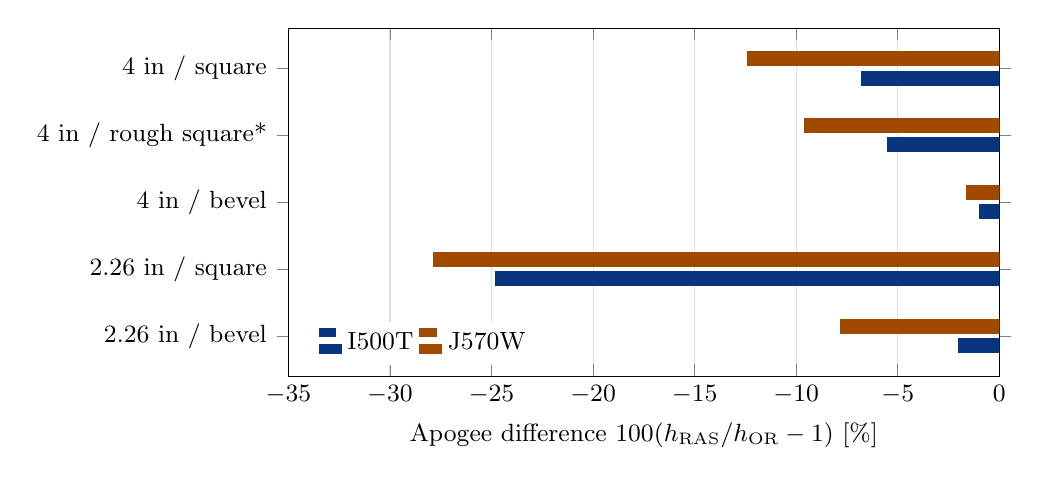
\begin{tikzpicture}
\begin{axis}[width=.875\textwidth,height=6.0cm,xbar,bar width=5pt,
xmin=-35,xmax=0,ymin=-.6,ymax=4.6,ytick={0,1,2,3,4},
yticklabels={4 in / square,4 in / rough square*,4 in / bevel,2.26 in / square,2.26 in / bevel},
y dir=reverse,xlabel={Apogee difference $100(h_{\mathrm{RAS}}/h_{\mathrm{OR}}-1)$ [\%]},
legend style={at={(.03,.03)},anchor=south west,draw=none,fill=white},legend columns=2,
axis on top=false,xmajorgrids=true,ymajorgrids=false,grid style={gray!25},font=\small]
\addplot[fill=B,draw=B] coordinates {(-6.7625130,0) (-5.5115726,1) (-0.9885049,2) (-24.7803734,3) (-1.9938998,4)};
\addlegendentry{I500T}
\addplot[fill=burntorange,draw=burntorange] coordinates {(-12.4019511,0) (-9.6082794,1) (-1.6076947,2) (-27.8381644,3) (-7.8064549,4)};
\addlegendentry{J570W}
\end{axis}\end{tikzpicture}
\caption{Apogee differences after matching geometry and fully turbulent flow. B02 (asterisk) retains a numerical roughness mismatch and is excluded from clean solver attribution.}\label{fig:apogee}
\end{figure}

* The rough-finish design B02 has unequal numerical roughness and is excluded from clean simulation attribution. Negative values mean RASAero predicts a lower apogee. All primary RASAero runs have All Turbulent Flow enabled.


\subsection{What the study establishes}

Replacing only MIT OR's drag coefficient with the curve recorded by RASAero reduces the eight clean apogee differences to \textbf{0.04-0.86\%}. This supports drag modeling as the dominant cause. It does not determine which program better predicts real flight; no flight measurements were used.


Three export issues need attention: turbulent-flow settings, beveled-fin geometry, and physical roughness mapping. A separate MIT time-step override is confirmed, but actual half-step refinement changes apogee by less than 0.02\% here.


\textbf{Aerodynamic follow-up.} Section~\ref{sec:aero} separates body and net fin contributions. It identifies a near-zero tangent-ogive nose-pressure term, loss of bevel sensitivity in the detached-shock fallback, and a body-length dependence in fin friction. An independent nose-term trial reduces mean absolute body-drag error by 84\% over six configurations at Mach 1.32--3. No MIT OR application/source changes were made.

RASAero was configured, run and exported through the Windows GUI. MIT OR used the installed MIT application JAR through its simulation/export APIs; all ten baseline cases and ten requested-step repeats were also run inside the VM. Mac/Windows apogees match exactly. This is a flight-prediction study, not a computational-speed benchmark.


\textbf{Completed extension.} Section~\ref{sec:extended} expands the data to 92 configurations and 82,800 common Mach/angle points, with 42 plot sheets. It tests nose shapes, fin geometry, physical roughness, transition, nozzle area, scale, normal force and CP without modifying the installed OR engine.

\clearpage\section{Experimental design}

The rockets deliberately remove appendages, active control and multi-stage complications. B01/B03 and B04/B05 isolate fin-edge treatment at fixed planform and mass. B02 exposes the roughness mapping problem. These are simulation fixtures, not qualified flight hardware designs.


{\small\setlength{\tabcolsep}{3pt}\renewcommand{\arraystretch}{1.16}
\begin{longtable}{@{}L{0.320\textwidth}L{0.310\textwidth}L{0.310\textwidth}@{}}
\caption{Nominal geometry and dry mass properties.}\label{tab:geometry}\\
\toprule
\textbf{Parameter} & \textbf{B01 / B02 / B03} & \textbf{B04 / B05}\\
\midrule\endfirsthead
\multicolumn{3}{l}{\small\itshape Table \thetable\ continued}\\
\toprule
\textbf{Parameter} & \textbf{B01 / B02 / B03} & \textbf{B04 / B05}\\
\midrule\endhead
\bottomrule\endfoot
Body diameter & 4.000 in (101.60 mm) & 2.260 in (57.404 mm)\\
Overall length & 60.000 in (1.524 m) & 50.000 in (1.270 m)\\
Tangent-ogive nose / body & 12 / 48 in & 10 / 40 in\\
Fins: count; root / tip chord & 4; 6 / 2 in & 3; 5 / 2 in\\
Fin span / leading-edge sweep & 3.25 / 4 in & 2.5 / 2.5 in\\
Thickness; aft-edge inset & 0.125 in; 0.500 in & 0.125 in; 0.500 in\\
Dry structure mass / dry CG & 6.000 kg / 33 in from tip & 1.000 kg / 27 in from tip\\
\end{longtable}}

{\small\setlength{\tabcolsep}{3pt}\renewcommand{\arraystretch}{1.16}
\begin{longtable}{@{}L{0.230\textwidth}L{0.340\textwidth}L{0.370\textwidth}@{}}
\caption{Design matrix and fin-edge treatment.}\label{tab:designs}\\
\toprule
\textbf{Design} & \textbf{Surface finish} & \textbf{Fin section}\\
\midrule\endfirsthead
\multicolumn{3}{l}{\small\itshape Table \thetable\ continued}\\
\toprule
\textbf{Design} & \textbf{Surface finish} & \textbf{Fin section}\\
\midrule\endhead
\bottomrule\endfoot
B01 smooth square & Zero roughness & Square\\
B02 rough square * & OR 60 micrometers; RAS 30.48 micrometers & Square\\
B03 smooth bevel & Zero roughness & 0.25 in nose bevel; square trailing edge\\
B04 slender square & Zero roughness & Square\\
B05 slender bevel & Zero roughness & 0.25 in nose bevel; square trailing edge\\
\end{longtable}}

\subsection{Shared flight conditions}

AeroTech I500T-14A and J570W use the same numerical RASP motor entries, preserved in models/study-motors.eng. Motors are aft-flush with zero overhang and no ignition delay. Dry mass/CG overrides include the structure and recovery system; motor mass and CG are added separately.


Launch altitude 0 m; vertical 2 m rail; zero wind and turbulence; 15 C and 101325 Pa at sea level. MIT OR uses ISA, latitude 45 degrees, longitude 0 and flat-earth geometry. RASAero receives 59 F, 29.9214 inHg and a 6.5617 ft rail. Both use a 24 in parachute, Cd 0.8, at apogee with no delay. Motor ejection is disabled in OR.


No lugs, rail guides, camera pods, tabs, fillets, transitions, fin cant, drag overrides or controllers. RASAero nozzle diameter is zero in these flight runs; later aerodynamic-only probes vary it to examine power-on/off drag sensitivity. Primary runs match the fully turbulent assumption: OR perfectFinish=false; RAS All Turbulent Flow=true.


\clearpage\section{Model equivalence and remaining differences}

{\small\setlength{\tabcolsep}{3pt}\renewcommand{\arraystretch}{1.16}
\begin{longtable}{@{}L{0.160\textwidth}L{0.440\textwidth}L{0.340\textwidth}@{}}
\caption{Model-equivalence audit and remaining implementation differences.}\label{tab:audit}\\
\toprule
\textbf{Item} & \textbf{Observed difference / treatment} & \textbf{Consequence}\\
\midrule\endfirsthead
\multicolumn{3}{l}{\small\itshape Table \thetable\ continued}\\
\toprule
\textbf{Item} & \textbf{Observed difference / treatment} & \textbf{Consequence}\\
\midrule\endhead
\bottomrule\endfoot
Fin-section export & MIT TRIANGULAR exports as Square with a warning. In the GUI, B03/B05 were changed to Hexagonal Blunt Base, FX1=0.25 in, LE radius=0. & Primary bevel runs preserve the pointed leading bevel and blunt trailing edge. Raw exports are retained.\\
Flow assumption & Exporter writes Turbulence=False; MIT OR uses perfectFinish=false. All Turbulent Flow was enabled in RAS for every primary case. & A settings mismatch is removed before solver attribution. Default-flow runs are retained as sensitivity data.\\
Surface roughness & B02: OR NORMAL=60 micrometers; RAS Rough Camouflage Paint=0.0012 in=30.48 micrometers. All other designs use zero. & B02 is a mapping diagnostic, not an equivalent-model comparison.\\
Geometry and units & RAS body length is rounded down by 0.0001 in. Other checked external dimensions match the export. & 2.54 micrometer length rounding is negligible at the displayed precision.\\
Mass and CG & OR retains components and motors; RAS uses entered launch mass/CG and motor data. Launch errors \textless{}0.023 g and \textless{}0.003 mm. & Initial mass properties match closely. Exported burn mass histories still differ by up to 2.28 g / 6.00 g for I500 / J570.\\
Dynamics & RAS no-wind mode is 2DOF; MIT OR retains its dynamics solver. RAS ascent angle of attack is exactly zero. & This axial benchmark does not compare wind response, damping, CP accuracy or control dynamics.\\
Atmosphere / gravity & ISA versus RAS U.S. Standard Atmosphere implementation; equal sea-level inputs. OR explicitly uses flat geometry. & Implementations and numerical evaluation remain possible sources of sub-percent residuals.\\
Sampling / integration & RAS CSV requested every 0.01 s; OR actual step is about 0.0025 s. RAS Mach, velocity and force columns show sample staggering. & Use direct exported peaks and explicitly matched Mach for aerodynamic comparisons; avoid inferring atmosphere from row-wise force balance.\\
Recovery / internals & Same nominal chute diameter, Cd and apogee trigger. Construction/inertia details are aggregated in RAS. & Ascent metrics are primary. Descent and landing loads are not validated.\\
\end{longtable}}

RASAero was run with a per-process English number-format launcher to avoid the VM locale misreading decimal points. The installed application binary and global Windows locale were not modified. The saved native files and CSV outputs were checked for valid decimal values.


\clearpage\section{Flight statistics}

Primary results: fully turbulent in both programs. Heights are above launch level (also MSL here). Maximum speed and Mach are ascent values. Percent difference is 100 x (RAS / OR - 1). I500 denotes the exact I500T-14A curve.


\begin{equation}\delta_h=100\left(\frac{h_{\mathrm{RAS}}}{h_{\mathrm{OR}}}-1\right)\,\%.\label{eq:apogee-difference}\end{equation}

{\small\setlength{\tabcolsep}{3pt}\renewcommand{\arraystretch}{1.16}
\begin{longtable}{@{}L{0.070\textwidth}L{0.100\textwidth}L{0.220\textwidth}L{0.120\textwidth}L{0.220\textwidth}L{0.210\textwidth}@{}}
\caption{Primary ascent performance. Percent differences use MIT OR as denominator.}\label{tab:flight}\\
\toprule
\textbf{Case} & \textbf{Motor} & \textbf{Apogee OR / RAS (m)} & \textbf{Difference} & \textbf{Max speed OR / RAS (m/s)} & \textbf{Max Mach OR / RAS}\\
\midrule\endfirsthead
\multicolumn{6}{l}{\small\itshape Table \thetable\ continued}\\
\toprule
\textbf{Case} & \textbf{Motor} & \textbf{Apogee OR / RAS (m)} & \textbf{Difference} & \textbf{Max speed OR / RAS (m/s)} & \textbf{Max Mach OR / RAS}\\
\midrule\endhead
\bottomrule\endfoot
B01 & I500T & 376.2 / 350.8 & -6.76\% & 82.4 / 81.7 & 0.242 / 0.240\\
B01 & J570W & 889.6 / 779.3 & -12.40\% & 131.7 / 128.5 & 0.388 / 0.378\\
B02 * & I500T & 369.7 / 349.3 & -5.51\% & 82.2 / 81.6 & 0.242 / 0.240\\
B02 * & J570W & 851.8 / 769.9 & -9.61\% & 130.6 / 128.1 & 0.385 / 0.377\\
B03 & I500T & 380.4 / 376.6 & -0.99\% & 82.6 / 82.5 & 0.243 / 0.242\\
B03 & J570W & 910.9 / 896.3 & -1.61\% & 132.3 / 131.9 & 0.389 / 0.388\\
B04 & I500T & 2027.4 / 1525.0 & -24.78\% & 364.5 / 349.7 & 1.074 / 1.030\\
B04 & J570W & 2811.8 / 2029.1 & -27.84\% & 479.6 / 437.4 & 1.417 / 1.291\\
B05 & I500T & 2252.6 / 2207.7 & -1.99\% & 369.6 / 368.5 & 1.089 / 1.086\\
B05 & J570W & 3076.2 / 2836.0 & -7.81\% & 486.1 / 463.8 & 1.436 / 1.370\\
\end{longtable}}

{\small\setlength{\tabcolsep}{3pt}\renewcommand{\arraystretch}{1.16}
\begin{longtable}{@{}L{0.100\textwidth}L{0.120\textwidth}L{0.340\textwidth}L{0.380\textwidth}@{}}
\caption{Time to apogee and maximum ascent acceleration.}\label{tab:time}\\
\toprule
\textbf{Case} & \textbf{Motor} & \textbf{Time to apogee OR / RAS (s)} & \textbf{Peak ascent acceleration OR / RAS (m/s$^2$)}\\
\midrule\endfirsthead
\multicolumn{4}{l}{\small\itshape Table \thetable\ continued}\\
\toprule
\textbf{Case} & \textbf{Motor} & \textbf{Time to apogee OR / RAS (s)} & \textbf{Peak ascent acceleration OR / RAS (m/s$^2$)}\\
\midrule\endhead
\bottomrule\endfoot
B01 & I500T & 9.195 / 8.790 & 78.38 / 77.64\\
B01 & J570W & 13.612 / 12.490 & 157.27 / 157.14\\
B02 * & I500T & 9.098 / 8.770 & 78.38 / 77.64\\
B02 * & J570W & 13.255 / 12.410 & 157.27 / 157.14\\
B03 & I500T & 9.258 / 9.190 & 78.38 / 77.64\\
B03 & J570W & 13.817 / 13.650 & 157.27 / 157.14\\
B04 & I500T & 17.160 / 14.080 & 358.30 / 354.87\\
B04 & J570W & 19.028 / 15.260 & 603.06 / 601.29\\
B05 & I500T & 18.373 / 17.960 & 358.41 / 357.32\\
B05 & J570W & 20.318 / 19.430 & 603.07 / 601.32\\
\end{longtable}}

* B02 is not matched in roughness. Its numbers are included for completeness, not to rank aerodynamic solvers. Peak acceleration is especially sensitive to output sampling and should not be interpreted as independently validated loading. Native RAS summary apogees agree with all ten CSV-derived apogees within 0.005 m.


\clearpage\section{Drag-model evidence}

MIT OR's installed aerodynamic calculator was evaluated at RASAero's reported Mach, altitude and zero angle of attack along ascent, using OR's ISA atmosphere. The plots show the J570 coast branch above 30 m/s. Matching Mach explicitly avoids the export's Mach/velocity sample offset. Residual atmosphere/Reynolds differences remain.


\begin{figure}[H]\centering
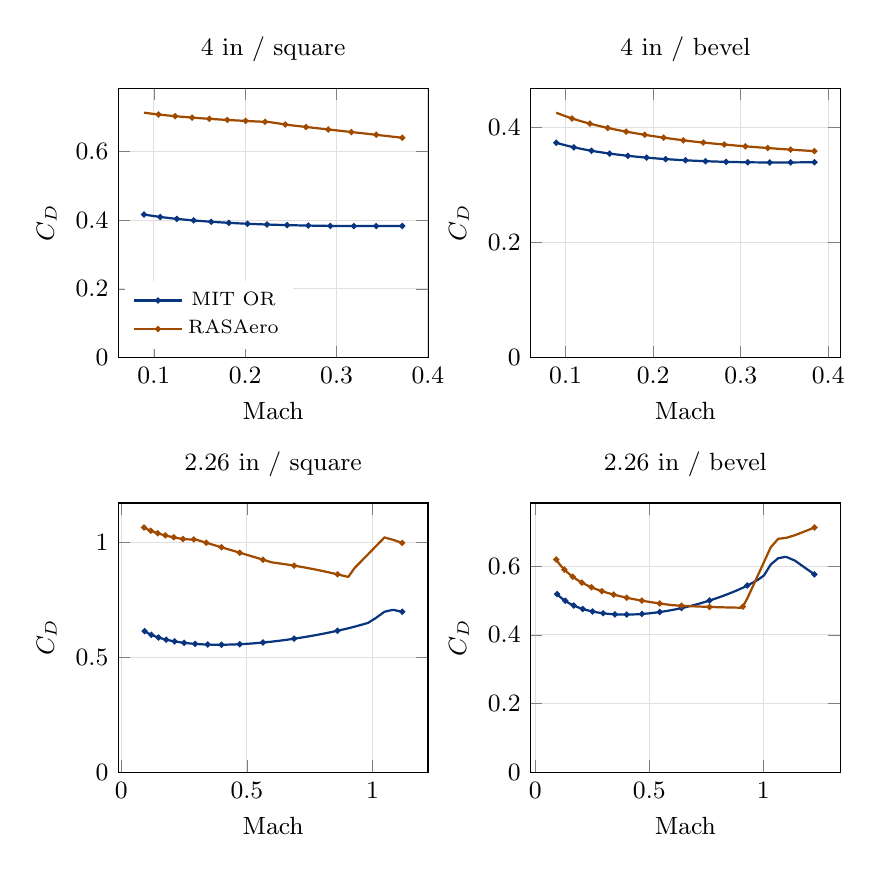
\begin{tikzpicture}
\begin{groupplot}[group style={group size=2 by 2,horizontal sep=1.3cm,vertical sep=1.85cm},
width=.455\textwidth,height=5.0cm,xlabel={Mach},ylabel={$C_D$},ymin=0,
grid=major,grid style={gray!25},tick label style={font=\small},label style={font=\small},title style={font=\small},
legend style={font=\scriptsize,draw=none,fill=white,at={(.02,.03)},anchor=south west}]
\nextgroupplot[title={4 in / square}]
\addplot[B,thick,mark=*,mark size=.65pt,mark repeat=10] coordinates {(0.3718897,0.3834246) (0.3693191,0.3833732) (0.3662538,0.3833167) (0.3632094,0.3832658) (0.3601856,0.3832205) (0.3576813,0.383187) (0.3546947,0.3831518) (0.3517278,0.383122) (0.3487805,0.3830975) (0.3463392,0.3830812) (0.3434271,0.3830664) (0.3405337,0.3830568) (0.337659,0.3830523) (0.3367048,0.3830519) (0.3352773,0.3830525) (0.332436,0.3830573) (0.3296125,0.3830672) (0.3268065,0.383082) (0.3244815,0.3830981) (0.3217072,0.3831219) (0.3189499,0.3831506) (0.3162092,0.383184) (0.3139379,0.3832156) (0.3112273,0.3832578) (0.3085327,0.3833048) (0.305854,0.3833564) (0.3036337,0.383403) (0.3009835,0.3834632) (0.2983485,0.383528) (0.2957286,0.3835974) (0.2931235,0.3836714) (0.2909637,0.3837365) (0.2883853,0.3838189) (0.2858211,0.3839057) (0.2832711,0.383997) (0.2811566,0.3840766) (0.2786319,0.3841762) (0.2761207,0.3842802) (0.2736228,0.3843887) (0.2715513,0.3844826) (0.2690775,0.3845993) (0.2666165,0.3847204) (0.2641683,0.384846) (0.2621376,0.384954) (0.2597121,0.3850878) (0.2572988,0.3852259) (0.2548976,0.3853686) (0.2529056,0.3854908) (0.250526,0.3856416) (0.248158,0.3857969) (0.2458011,0.3859567) (0.2438456,0.3860933) (0.241509,0.3862614) (0.2391832,0.386434) (0.2368681,0.3866111) (0.2345636,0.3867923) (0.232651,0.3869465) (0.2303655,0.3871357) (0.22809,0.3873297) (0.2258246,0.3875283) (0.2239445,0.3876974) (0.2216977,0.3879046) (0.2194611,0.3881165) (0.2172344,0.3883332) (0.2153863,0.3885175) (0.2131774,0.388743) (0.2109781,0.3889733) (0.2087881,0.3892086) (0.2069703,0.3894085) (0.2047971,0.3896529) (0.2026331,0.3899024) (0.2004778,0.390157) (0.1986884,0.3903731) (0.1965491,0.3906372) (0.1944182,0.3909066) (0.1922957,0.3911813) (0.1905333,0.3914143) (0.1884257,0.391699) (0.1863262,0.3919893) (0.1842346,0.3922851) (0.1821508,0.3925867) (0.18042,0.3928424) (0.1783501,0.3931547) (0.1762876,0.3934729) (0.1742324,0.3937971) (0.1725253,0.3940721) (0.1704832,0.3944077) (0.1684481,0.3947497) (0.1664199,0.3950982) (0.164735,0.3953936) (0.1627191,0.3957543) (0.1607099,0.3961217) (0.1587072,0.3964962) (0.1570431,0.3968136) (0.155052,0.3972012) (0.1530671,0.3975962) (0.1510883,0.3979987) (0.1494438,0.39834) (0.147476,0.3987568) (0.1455139,0.3991816) (0.1435576,0.3996147) (0.1419317,0.399982) (0.1399856,0.4004307) (0.138045,0.4008882) (0.1361098,0.4013547) (0.1341799,0.4018305) (0.1325756,0.4022343) (0.1306551,0.4027278) (0.1287397,0.4032313) (0.1268292,0.4037452) (0.1252409,0.4041814) (0.1233393,0.404715) (0.1214424,0.4052597) (0.1195501,0.4058159) (0.1179767,0.4062885) (0.1160927,0.4068669) (0.114213,0.4074579) (0.1123378,0.4080619) (0.1107782,0.4085755) (0.1089106,0.4092046) (0.1070471,0.409848) (0.1051876,0.4105063) (0.103641,0.4110667) (0.1017887,0.4117536) (0.09994016,0.4124571) (0.09809534,0.4131778) (0.09656077,0.4137919) (0.09472257,0.4145457) (0.09288788,0.4153188) (0.09105664,0.4161119) (0.08922875,0.4169258)};
\addlegendentry{MIT OR}
\addplot[burntorange,thick,mark=*,mark size=.65pt,mark repeat=10] coordinates {(0.3718897,0.6409085) (0.3693191,0.6416892) (0.3662538,0.6426184) (0.3632094,0.6435403) (0.3601856,0.6444545) (0.3576813,0.6452107) (0.3546947,0.6461117) (0.3517278,0.6470054) (0.3487805,0.6478924) (0.3463392,0.6486263) (0.3434271,0.6495012) (0.3405337,0.6503692) (0.337659,0.6512311) (0.3352773,0.6519445) (0.332436,0.6527948) (0.3296125,0.6536394) (0.3268065,0.654478) (0.3244815,0.6551725) (0.3217072,0.6560007) (0.3189499,0.6568233) (0.3162092,0.6576409) (0.3139379,0.6583179) (0.3112273,0.6591256) (0.3085327,0.6599285) (0.305854,0.6607264) (0.3036337,0.6613876) (0.3009835,0.6621769) (0.2983485,0.6629613) (0.2957286,0.6637415) (0.2931235,0.6645173) (0.2909637,0.6651605) (0.2883853,0.6659286) (0.2858211,0.6666925) (0.2832711,0.6674528) (0.2811566,0.6680831) (0.2786319,0.6688362) (0.2761207,0.6695858) (0.2736228,0.6703317) (0.2715513,0.6709506) (0.2690775,0.6716905) (0.2666165,0.6724268) (0.2641683,0.6731602) (0.2621376,0.6737689) (0.2597121,0.6744968) (0.2572988,0.6752218) (0.2548976,0.6759439) (0.2529056,0.6765436) (0.250526,0.6772612) (0.248158,0.6781347) (0.2458011,0.679051) (0.2438456,0.6798127) (0.241509,0.6807246) (0.2391832,0.6816339) (0.2368681,0.6825414) (0.2345636,0.6834463) (0.232651,0.6841991) (0.2303655,0.6851006) (0.22809,0.6860004) (0.2258246,0.6868517) (0.2239445,0.6870721) (0.2216977,0.6873384) (0.2194611,0.6876068) (0.2172344,0.6878772) (0.2153863,0.6881043) (0.2131774,0.6883788) (0.2109781,0.6886556) (0.2087881,0.6889346) (0.2069703,0.689169) (0.2047971,0.6894525) (0.2026331,0.6897385) (0.2004778,0.690027) (0.1986884,0.6902695) (0.1965491,0.6905628) (0.1944182,0.6908589) (0.1922957,0.6911578) (0.1905333,0.6914091) (0.1884257,0.6917134) (0.1863262,0.6920206) (0.1842346,0.692331) (0.1821508,0.6926444) (0.18042,0.6929082) (0.1783501,0.6932277) (0.1762876,0.6935506) (0.1742324,0.6938771) (0.1725253,0.6941519) (0.1704832,0.694485) (0.1684481,0.6948219) (0.1664199,0.6951627) (0.164735,0.6954497) (0.1627191,0.6957979) (0.1607099,0.6961502) (0.1587072,0.6965069) (0.1570431,0.6968076) (0.155052,0.6971725) (0.1530671,0.6975421) (0.1510883,0.6979165) (0.1494438,0.6982324) (0.147476,0.698616) (0.1455139,0.6990048) (0.1435576,0.6993991) (0.1419317,0.6997319) (0.1399856,0.7001365) (0.138045,0.700547) (0.1361098,0.7009636) (0.1341799,0.7013864) (0.1325756,0.7017437) (0.1306551,0.7021786) (0.1287397,0.7026204) (0.1268292,0.7030693) (0.1252409,0.7034489) (0.1233393,0.7039114) (0.1214424,0.7043818) (0.1195501,0.7048603) (0.1179767,0.7052655) (0.1160927,0.7057596) (0.114213,0.7062627) (0.1123378,0.7067751) (0.1107782,0.7072095) (0.1089106,0.7077399) (0.1070471,0.7082807) (0.1051876,0.7088322) (0.103641,0.7093004) (0.1017887,0.7098728) (0.09994016,0.7104573) (0.09809534,0.7110544) (0.09656077,0.711562) (0.09472257,0.7121837) (0.09288788,0.7128195) (0.09105664,0.7134701) (0.08922875,0.7141363)};
\addlegendentry{RASAero}
\nextgroupplot[title={4 in / bevel}]
\addplot[B,thick,mark=*,mark size=.65pt,mark repeat=10] coordinates {(0.3842369,0.3397753) (0.3817109,0.3397157) (0.3787768,0.3396507) (0.3762731,0.3395989) (0.3733648,0.3395431) (0.37047,0.3394921) (0.3679993,0.3394523) (0.3651292,0.3394104) (0.3622721,0.3393732) (0.3598334,0.3393452) (0.3570001,0.3393169) (0.3541793,0.3392933) (0.3517713,0.3392768) (0.3489734,0.339262) (0.3461877,0.3392517) (0.3438093,0.3392467) (0.3414396,0.339245) (0.3410456,0.3392451) (0.3386859,0.3392474) (0.3359437,0.3392543) (0.3332128,0.3392659) (0.3308811,0.3392794) (0.328171,0.3392994) (0.3254718,0.339324) (0.3231669,0.3393487) (0.3204877,0.3393817) (0.3178191,0.3394192) (0.3155401,0.3394549) (0.3128907,0.3395008) (0.3102517,0.3395513) (0.3079975,0.3395981) (0.305377,0.3396569) (0.3031386,0.3397109) (0.3005362,0.3397781) (0.2979434,0.3398498) (0.2957284,0.3399149) (0.2931531,0.3399951) (0.290587,0.3400797) (0.2883947,0.3401559) (0.2858455,0.3402491) (0.2833051,0.3403468) (0.2811347,0.3404342) (0.2786106,0.3405404) (0.2760951,0.3406511) (0.2739456,0.3407488) (0.2714458,0.3408671) (0.2693097,0.3409722) (0.2668251,0.3410992) (0.2643486,0.3412309) (0.2622323,0.3413475) (0.2597705,0.3414881) (0.2573166,0.3416334) (0.2552194,0.3417619) (0.2527796,0.3419162) (0.2503474,0.3420754) (0.2482685,0.3422159) (0.24585,0.3423843) (0.2434386,0.3425577) (0.2413773,0.3427104) (0.238979,0.3428933) (0.2369289,0.3430541) (0.2345434,0.3432466) (0.2321646,0.3434443) (0.230131,0.343618) (0.2277647,0.3438255) (0.2254048,0.3440385) (0.2233872,0.3442254) (0.2210392,0.3444485) (0.2186975,0.3446773) (0.2166953,0.3448779) (0.2143651,0.3451172) (0.2120409,0.3453623) (0.2100535,0.3455771) (0.2077404,0.3458331) (0.2057623,0.3460575) (0.2034599,0.3463248) (0.2011631,0.3465984) (0.199199,0.346838) (0.1969127,0.3471233) (0.1946318,0.3474152) (0.192681,0.3476707) (0.1904101,0.3479749) (0.1881444,0.348286) (0.1862065,0.3485581) (0.1839505,0.3488822) (0.1816994,0.3492135) (0.1797739,0.3495033) (0.1775321,0.3498484) (0.1756144,0.3501502) (0.1733815,0.3505095) (0.1711534,0.3508768) (0.1692473,0.351198) (0.1670278,0.3515804) (0.1648128,0.3519713) (0.1629177,0.3523132) (0.160711,0.3527203) (0.1585086,0.3531364) (0.1566243,0.3535004) (0.1544298,0.3539339) (0.1522395,0.3543771) (0.1503654,0.3547649) (0.1481827,0.3552267) (0.146315,0.3556309) (0.1441396,0.3561125) (0.1419681,0.3566051) (0.1401099,0.3570363) (0.1379455,0.3575502) (0.1357847,0.3580761) (0.1339356,0.3585366) (0.1317816,0.3590858) (0.1296311,0.359648) (0.1277906,0.3601407) (0.1256465,0.3607285) (0.1235058,0.3613307) (0.1216736,0.3618587) (0.119539,0.362489) (0.1177119,0.3630419) (0.1155832,0.3637022) (0.1134576,0.3643797) (0.1116381,0.3649744) (0.1095181,0.3656854) (0.1074011,0.3664154) (0.1055888,0.3670569) (0.1034771,0.3678245) (0.1013681,0.3686137) (0.09956264,0.3693079) (0.09745872,0.3701396) (0.09535743,0.3709957) (0.09355838,0.3717498) (0.09146181,0.3726545) (0.08936773,0.3735871)};
\addplot[burntorange,thick,mark=*,mark size=.65pt,mark repeat=10] coordinates {(0.3842369,0.3589948) (0.3817109,0.3592286) (0.3787768,0.3595025) (0.3762731,0.3597384) (0.3733648,0.3600148) (0.37047,0.3602926) (0.3679993,0.3605319) (0.3651292,0.3608124) (0.3622721,0.3610942) (0.3598334,0.3613371) (0.3570001,0.3616217) (0.3541793,0.361908) (0.3517713,0.3621546) (0.3489734,0.3624438) (0.3461877,0.3627346) (0.3438093,0.3629851) (0.3410456,0.363279) (0.3386859,0.3635323) (0.3359437,0.3638295) (0.3332128,0.3641284) (0.3308811,0.3643861) (0.328171,0.3646884) (0.3254718,0.3649926) (0.3231669,0.3652548) (0.3204877,0.3655627) (0.3178191,0.3658725) (0.3155401,0.3661396) (0.3128907,0.3664533) (0.3102517,0.366769) (0.3079975,0.3670413) (0.305377,0.3673611) (0.3031386,0.3676369) (0.3005362,0.3679609) (0.2979434,0.3682871) (0.2957284,0.3685686) (0.2931531,0.3688993) (0.290587,0.3692324) (0.2883947,0.36952) (0.2858455,0.3698578) (0.2833051,0.3701982) (0.2811347,0.3704922) (0.2786106,0.3708376) (0.2760951,0.3711857) (0.2739456,0.3714865) (0.2714458,0.3718399) (0.2693097,0.3721452) (0.2668251,0.3725041) (0.2643486,0.3728661) (0.2622323,0.3731788) (0.2597705,0.3735467) (0.2573166,0.3739178) (0.2552194,0.3742384) (0.2527796,0.3746157) (0.2503474,0.3749964) (0.2482685,0.3753587) (0.24585,0.3757924) (0.2434386,0.3762299) (0.2413773,0.376608) (0.238979,0.3770526) (0.2369289,0.3774369) (0.2345434,0.3778891) (0.2321646,0.3783454) (0.230131,0.3787399) (0.2277647,0.3792042) (0.2254048,0.379673) (0.2233872,0.3800784) (0.2210392,0.3805557) (0.2186975,0.3810378) (0.2166953,0.3814549) (0.2143651,0.3819462) (0.2120409,0.3824426) (0.2100535,0.3828723) (0.2077404,0.3833786) (0.2057623,0.3838169) (0.2034599,0.3843335) (0.2011631,0.3848559) (0.199199,0.3853083) (0.1969127,0.3858418) (0.1946318,0.3863815) (0.192681,0.3868492) (0.1904101,0.3874009) (0.1881444,0.3879594) (0.1862065,0.3884435) (0.1839505,0.3890149) (0.1816994,0.3895935) (0.1797739,0.3900955) (0.1775321,0.3906882) (0.1756144,0.3912024) (0.1733815,0.39181) (0.1711534,0.3924257) (0.1692473,0.3929604) (0.1670278,0.3935923) (0.1648128,0.3942332) (0.1629177,0.39479) (0.160711,0.3954485) (0.1585086,0.3961169) (0.1566243,0.3966978) (0.1544298,0.3973854) (0.1522395,0.3980837) (0.1503654,0.3986912) (0.1481827,0.3994105) (0.146315,0.4000366) (0.1441396,0.4007783) (0.1419681,0.4015327) (0.1401099,0.4021897) (0.1379455,0.4029687) (0.1357847,0.4037617) (0.1339356,0.4044529) (0.1317816,0.4052732) (0.1296311,0.406109) (0.1277906,0.4068382) (0.1256465,0.4077044) (0.1235058,0.4085878) (0.1216736,0.4093593) (0.119539,0.4102767) (0.1177119,0.4110783) (0.1155832,0.4120323) (0.1134576,0.4130071) (0.1116381,0.4138599) (0.1095181,0.4148759) (0.1074011,0.4159155) (0.1055888,0.4168262) (0.1034771,0.4179126) (0.1013681,0.4190258) (0.09956264,0.4200024) (0.09745872,0.421169) (0.09535743,0.4223664) (0.09355838,0.4234185) (0.09146181,0.4246774) (0.08936773,0.4259719)};
\nextgroupplot[title={2.26 in / square}]
\addplot[B,thick,mark=*,mark size=.65pt,mark repeat=10] coordinates {(1.117796,0.6989336) (1.083895,0.7071794) (1.079184,0.7075247) (1.047065,0.6991513) (1.012991,0.6723016) (0.9820645,0.6507732) (0.9538127,0.6419407) (0.9278567,0.634213) (0.9040796,0.627456) (0.8818073,0.6217561) (0.8604159,0.6165587) (0.8398563,0.6117454) (0.8200874,0.6072864) (0.80107,0.6031545) (0.7827664,0.5993246) (0.7651408,0.5957722) (0.7481591,0.5924753) (0.731789,0.5894172) (0.7179427,0.5869234) (0.7026377,0.5842668) (0.6878604,0.5818022) (0.6735846,0.5795159) (0.6597858,0.5773952) (0.6464405,0.5754285) (0.6335267,0.5736052) (0.6210237,0.5719156) (0.6089118,0.5703505) (0.5971723,0.5689018) (0.585774,0.5675601) (0.5746944,0.566318) (0.5639202,0.5651696) (0.553439,0.5641093) (0.5432389,0.5631321) (0.5333084,0.5622332) (0.5248321,0.5615074) (0.5153787,0.5607438) (0.5061653,0.5600465) (0.4971824,0.5594121) (0.4884211,0.5588371) (0.479873,0.5583185) (0.4715297,0.5578533) (0.4633836,0.5574388) (0.4554272,0.5570723) (0.4476535,0.5567517) (0.4400557,0.5564745) (0.4326274,0.5562388) (0.4253623,0.5560425) (0.4182545,0.555884) (0.4112985,0.5557614) (0.4044889,0.5556704) (0.3986465,0.5556176) (0.3920977,0.555587) (0.388873,0.5555831) (0.3856809,0.5555867) (0.3793918,0.5556156) (0.3732259,0.5556724) (0.3671791,0.5557561) (0.3612473,0.5558658) (0.3554268,0.5560004) (0.349714,0.5561591) (0.3441051,0.556341) (0.3385969,0.5565454) (0.3331861,0.5567716) (0.3278697,0.557019) (0.3226445,0.5572868) (0.3175077,0.5575746) (0.3124565,0.5578817) (0.3081049,0.558166) (0.3032072,0.5585082) (0.2983877,0.5588685) (0.2936447,0.5592464) (0.2889783,0.5596414) (0.2843865,0.5600531) (0.2798667,0.5604812) (0.2754167,0.5609253) (0.2710341,0.5613854) (0.2667168,0.561861) (0.2624627,0.5623521) (0.2582698,0.5628584) (0.2541362,0.5633799) (0.2500601,0.5639164) (0.2460392,0.5644679) (0.2420714,0.5650343) (0.238642,0.5655422) (0.2347697,0.5661367) (0.2309461,0.5667461) (0.2271699,0.5673704) (0.2234396,0.5680098) (0.219754,0.5686642) (0.2161119,0.5693338) (0.2125118,0.5700187) (0.2089527,0.5707191) (0.2054334,0.571435) (0.2019528,0.5721668) (0.1985097,0.5729145) (0.1951033,0.5736784) (0.1917324,0.5744589) (0.188396,0.5752561) (0.1850932,0.5760704) (0.1822301,0.5767971) (0.1789879,0.5776444) (0.1757767,0.5785097) (0.1725956,0.5793936) (0.1694439,0.5802965) (0.1663207,0.5812189) (0.1632253,0.5821613) (0.1601568,0.5831242) (0.1571146,0.5841084) (0.154098,0.5851143) (0.1511062,0.5861427) (0.1481385,0.5871944) (0.1451944,0.5882701) (0.1422731,0.5893706) (0.139374,0.5904968) (0.1364966,0.5916498) (0.1339961,0.5926813) (0.1311575,0.5938871) (0.1283389,0.5951227) (0.1255396,0.5963894) (0.1227592,0.5976885) (0.1199971,0.5990214) (0.1172527,0.6003896) (0.1145256,0.6017949) (0.1118152,0.6032389) (0.1091211,0.6047236) (0.1064428,0.606251) (0.1037798,0.6078234) (0.1011316,0.6094432) (0.09849794,0.6111129) (0.09587819,0.6128354) (0.09327197,0.6146137) (0.09067889,0.6164513)};
\addplot[burntorange,thick,mark=*,mark size=.65pt,mark repeat=10] coordinates {(1.117796,0.9994134) (1.083895,1.012117) (1.047065,1.023195) (1.012991,0.9848054) (0.9820645,0.9500911) (0.9538127,0.9184952) (0.9278567,0.8895721) (0.9040796,0.852327) (0.9012413,0.8516064) (0.8818073,0.8566008) (0.8604159,0.8622884) (0.8398563,0.8675429) (0.8200874,0.8724013) (0.80107,0.8768976) (0.7827664,0.8810629) (0.7651408,0.8849248) (0.7481591,0.888509) (0.731789,0.8918389) (0.7179427,0.8945603) (0.7026377,0.8974683) (0.6878604,0.9001772) (0.6735846,0.9027031) (0.6597858,0.905061) (0.6464405,0.9072638) (0.6335267,0.9093241) (0.6210237,0.9112526) (0.6089118,0.9130595) (0.5971723,0.9152322) (0.585774,0.9190626) (0.5746944,0.922771) (0.5639202,0.9263633) (0.553439,0.9298455) (0.5432389,0.9332232) (0.5333084,0.9365016) (0.5248321,0.9392927) (0.5153787,0.9423981) (0.5061653,0.9454176) (0.4971824,0.9483555) (0.4884211,0.9512159) (0.479873,0.9540021) (0.4715297,0.9567178) (0.4633836,0.9593664) (0.4554272,0.9619512) (0.4476535,0.9644746) (0.4400557,0.9669399) (0.4326274,0.9693494) (0.4253623,0.971706) (0.4182545,0.9740118) (0.4112985,0.9762694) (0.4044889,0.9784807) (0.3986465,0.9803795) (0.3920977,0.9825094) (0.3856809,0.9845992) (0.3793918,0.9866499) (0.3732259,0.9886636) (0.3671791,0.990642) (0.3612473,0.9925865) (0.3554268,0.9944987) (0.349714,0.9963799) (0.3441051,0.9982316) (0.3385969,1.000055) (0.3331861,1.001851) (0.3278697,1.003622) (0.3226445,1.005368) (0.3175077,1.00709) (0.3124565,1.00879) (0.3081049,1.01026) (0.3032072,1.011921) (0.2983877,1.013563) (0.2936447,1.014235) (0.2889783,1.014304) (0.2843865,1.014385) (0.2798667,1.014479) (0.2754167,1.014584) (0.2710341,1.014702) (0.2667168,1.014832) (0.2624627,1.014973) (0.2582698,1.015126) (0.2541362,1.015291) (0.2500601,1.015468) (0.2460392,1.016188) (0.2420714,1.016922) (0.238642,1.017567) (0.2347697,1.01831) (0.2309461,1.019058) (0.2271699,1.019812) (0.2234396,1.020572) (0.219754,1.021338) (0.2161119,1.02211) (0.2125118,1.022889) (0.2089527,1.023676) (0.2054334,1.024469) (0.2019528,1.025271) (0.1985097,1.02608) (0.1951033,1.026899) (0.1917324,1.027725) (0.188396,1.028561) (0.1850932,1.029407) (0.1822301,1.030155) (0.1789879,1.03102) (0.1757767,1.031896) (0.1725956,1.032782) (0.1694439,1.033681) (0.1663207,1.034592) (0.1632253,1.035516) (0.1601568,1.036453) (0.1571146,1.037405) (0.154098,1.038371) (0.1511062,1.039352) (0.1481385,1.040349) (0.1451944,1.041363) (0.1422731,1.042395) (0.139374,1.043444) (0.1364966,1.044513) (0.1339961,1.045465) (0.1311575,1.046573) (0.1283389,1.047702) (0.1255396,1.048855) (0.1227592,1.050031) (0.1199971,1.051233) (0.1172527,1.052462) (0.1145256,1.053719) (0.1118152,1.055006) (0.1091211,1.056324) (0.1064428,1.057676) (0.1037798,1.059062) (0.1011316,1.060485) (0.09849794,1.061947) (0.09587819,1.063451) (0.09327197,1.064999) (0.09067889,1.066594)};
\nextgroupplot[title={2.26 in / bevel}]
\addplot[B,thick,mark=*,mark size=.65pt,mark repeat=10] coordinates {(1.224446,0.5764026) (1.179592,0.5970638) (1.138447,0.6165883) (1.100489,0.6273706) (1.097177,0.6274073) (1.065165,0.6234712) (1.032249,0.6048699) (1.002831,0.5731794) (0.9765267,0.5606116) (0.950776,0.5512044) (0.9294382,0.5438433) (0.9099175,0.5374382) (0.8915522,0.5318551) (0.8738523,0.52688) (0.8567569,0.522259) (0.8402321,0.5179599) (0.8228187,0.5136039) (0.8073875,0.5098904) (0.7924363,0.5064216) (0.7779403,0.5031782) (0.7638759,0.5001428) (0.7502216,0.4973) (0.736957,0.4946356) (0.7229086,0.4919177) (0.7103989,0.489587) (0.6982241,0.487398) (0.6863686,0.4853381) (0.674818,0.4834033) (0.6635586,0.4815859) (0.6525775,0.4798785) (0.6409013,0.4781337) (0.6304638,0.4766358) (0.6202694,0.4752292) (0.6103079,0.4739088) (0.6005697,0.47267) (0.5910441,0.471508) (0.5817196,0.4704185) (0.5717677,0.4693083) (0.5628393,0.4683589) (0.5540895,0.4674715) (0.5455118,0.4666432) (0.5371,0.4658713) (0.528848,0.4651532) (0.5207503,0.4644866) (0.5120861,0.4638153) (0.5042937,0.4632492) (0.4966397,0.4627281) (0.4891194,0.4622501) (0.4817282,0.4618134) (0.4744619,0.4614121) (0.4673163,0.4610492) (0.4602875,0.4607233) (0.4527486,0.4604085) (0.4459521,0.4601558) (0.4392613,0.4599363) (0.4326727,0.4597488) (0.4261834,0.4595925) (0.4197902,0.4594663) (0.4134901,0.4593694) (0.4067202,0.459296) (0.4006059,0.4592576) (0.3951211,0.4592459) (0.3945764,0.459246) (0.3886292,0.4592606) (0.3827618,0.4593007) (0.3769719,0.4593657) (0.3712573,0.4594552) (0.3651065,0.45958) (0.3595424,0.4597189) (0.3540471,0.4598807) (0.3486187,0.4600651) (0.3432553,0.4602717) (0.3379551,0.4605002) (0.3327164,0.4607502) (0.3270696,0.4610473) (0.321954,0.4613417) (0.3168948,0.4616569) (0.3118905,0.4619928) (0.3069397,0.4623492) (0.3020408,0.4627261) (0.2971925,0.4631233) (0.2919596,0.4635798) (0.2872128,0.4640193) (0.2825126,0.4644791) (0.2778578,0.4649592) (0.2732471,0.4654595) (0.2686794,0.46598) (0.2641537,0.466518) (0.2592629,0.4671285) (0.2548214,0.4677098) (0.2504184,0.4683122) (0.246053,0.4689358) (0.241724,0.4695809) (0.2374305,0.4702479) (0.2331716,0.4709369) (0.2289465,0.4716485) (0.2243748,0.4724508) (0.2202175,0.4732107) (0.2160914,0.4739944) (0.2119957,0.4748025) (0.2079296,0.4756355) (0.2038924,0.476494) (0.1998833,0.4773787) (0.195541,0.4783745) (0.1915884,0.4793163) (0.1876619,0.4802866) (0.1837606,0.4812864) (0.179884,0.4823166) (0.1760314,0.4833784) (0.1722021,0.4844727) (0.1680508,0.4857051) (0.1642685,0.4868716) (0.1605077,0.4880747) (0.1567679,0.489316) (0.1530485,0.4905972) (0.149349,0.49192) (0.1456688,0.4932863) (0.1416753,0.4948291) (0.1380337,0.4962935) (0.1344098,0.4978085) (0.1308031,0.4993769) (0.127213,0.5010016) (0.1236392,0.5026859) (0.120081,0.5044332) (0.1162168,0.5064159) (0.11269,0.5083082) (0.1091775,0.5102768) (0.1056788,0.512327) (0.1021935,0.5144647) (0.09872108,0.5166963) (0.0952612,0.5190291) (0.09150053,0.5216988)};
\addplot[burntorange,thick,mark=*,mark size=.65pt,mark repeat=10] coordinates {(1.224446,0.7129686) (1.179592,0.701018) (1.138447,0.690553) (1.100489,0.6827861) (1.065165,0.6800253) (1.032249,0.6549171) (1.002831,0.6122059) (0.9765267,0.5740452) (0.950776,0.5367184) (0.9294382,0.5058141) (0.9099175,0.482399) (0.8998074,0.4793066) (0.8915522,0.4794028) (0.8738523,0.4796245) (0.8567569,0.47986) (0.8402321,0.4801085) (0.8228187,0.4803934) (0.8073875,0.4806667) (0.7924363,0.4809509) (0.7779403,0.4812455) (0.7638759,0.4815501) (0.7502216,0.4818641) (0.736957,0.4821871) (0.7229086,0.4825494) (0.7103989,0.4828902) (0.6982241,0.483239) (0.6863686,0.4835956) (0.674818,0.4839596) (0.6635586,0.4843308) (0.6525775,0.4847091) (0.6409013,0.4851294) (0.6304638,0.4855218) (0.6202694,0.4859206) (0.6103079,0.4863258) (0.6005697,0.4867372) (0.5910441,0.4875006) (0.5817196,0.4883026) (0.5717677,0.4891784) (0.5628393,0.4899823) (0.5540895,0.4907873) (0.5455118,0.4915936) (0.5371,0.4924012) (0.528848,0.4932106) (0.5207503,0.4940215) (0.5120861,0.4949084) (0.5042937,0.4957235) (0.4966397,0.4965408) (0.4891194,0.4973606) (0.4817282,0.4981829) (0.4744619,0.4990078) (0.4673163,0.4998357) (0.4602875,0.5006666) (0.4527486,0.5015768) (0.4459521,0.5024147) (0.4392613,0.5032563) (0.4326727,0.5041017) (0.4261834,0.5049511) (0.4197902,0.5058047) (0.4134901,0.5066627) (0.4067202,0.507604) (0.4006059,0.5084719) (0.3945764,0.5093449) (0.3886292,0.5102232) (0.3827618,0.511107) (0.3769719,0.5119966) (0.3712573,0.5128922) (0.3651065,0.5138763) (0.3595424,0.5147853) (0.3540471,0.5157011) (0.3486187,0.5166239) (0.3432553,0.5175541) (0.3379551,0.5184919) (0.3327164,0.5194377) (0.3270696,0.5204789) (0.321954,0.5214423) (0.3168948,0.5224147) (0.3118905,0.5233964) (0.3069397,0.5243877) (0.3020408,0.5253889) (0.2971925,0.5264006) (0.2919596,0.5275166) (0.2872128,0.5285514) (0.2825126,0.5295978) (0.2778578,0.5306563) (0.2732471,0.5317275) (0.2686794,0.5328117) (0.2641537,0.5339096) (0.2592629,0.5351233) (0.2548214,0.5362513) (0.2504184,0.5373946) (0.246053,0.5386637) (0.241724,0.539961) (0.2374305,0.5412754) (0.2331716,0.5426078) (0.2289465,0.5439589) (0.2243748,0.5454552) (0.2202175,0.5468481) (0.2160914,0.5482623) (0.2119957,0.5496988) (0.2079296,0.5511585) (0.2038924,0.5526426) (0.1998833,0.5541522) (0.195541,0.5558292) (0.1915884,0.5573957) (0.1876619,0.5589914) (0.1837606,0.5606177) (0.179884,0.5622762) (0.1760314,0.5639683) (0.1722021,0.5656958) (0.1680508,0.5676227) (0.1642685,0.56943) (0.1605077,0.5712786) (0.1567679,0.5731705) (0.1530485,0.5751083) (0.149349,0.5770944) (0.1456688,0.5791315) (0.1416753,0.5814156) (0.1380337,0.5835692) (0.1344098,0.5857835) (0.1308031,0.5880626) (0.127213,0.5904102) (0.1236392,0.592831) (0.120081,0.5953296) (0.1162168,0.5981504) (0.11269,0.6008295) (0.1091775,0.6036045) (0.1056788,0.6064826) (0.1021935,0.6094714) (0.09872108,0.6125798) (0.0952612,0.6158174) (0.09150053,0.6195094)};
\end{groupplot}\end{tikzpicture}
\caption{J570W coast-branch drag at common reported Mach and altitude, above \SI{30}{m.s^{-1}}. MIT OR retains its ISA atmosphere. Curves are subsampled for display only; statistics use the full histories.}\label{fig:drag}
\end{figure}

{\small\setlength{\tabcolsep}{3pt}\renewcommand{\arraystretch}{1.16}
\begin{longtable}{@{}L{0.280\textwidth}L{0.220\textwidth}L{0.220\textwidth}L{0.220\textwidth}@{}}
\caption{Drag coefficient at the RASAero maximum-speed row, J570W cases.}\label{tab:cd}\\
\toprule
\textbf{J570 case} & \textbf{MIT OR Cd} & \textbf{RAS Cd} & \textbf{RAS / OR}\\
\midrule\endfirsthead
\multicolumn{4}{l}{\small\itshape Table \thetable\ continued}\\
\toprule
\textbf{J570 case} & \textbf{MIT OR Cd} & \textbf{RAS Cd} & \textbf{RAS / OR}\\
\midrule\endhead
\bottomrule\endfoot
B01 & 0.384 & 0.639 & 1.67\\
B03 & 0.340 & 0.359 & 1.06\\
B04 & 0.588 & 0.920 & 1.56\\
B05 & 0.550 & 0.785 & 1.43\\
\end{longtable}}

Table: coefficients at the RAS maximum-speed row, with OR evaluated at that row's reported Mach and altitude. Both coefficients use the body frontal reference area. These are comparisons of model predictions, not measured drag.


The square-fin discrepancies persist at common flight states, so they cannot be explained solely by the trajectories reaching different speeds. Beveling changes RASAero's predicted drag and apogee much more than MIT OR's in these fixtures. RAS component drag decomposition was not available in the flight export. The later aerodynamic investigation uses paired finless/finned fixtures to separate the net fin contribution; its internal pressure, friction and interference terms remain unreported by RAS.


\clearpage\section{Attribution and numerical checks}

\subsection{Replace drag; retain MIT OR's flight solver}

A diagnostic listener substitutes RASAero's trajectory-derived Cd(Mach) into OR's total and axial drag coefficients. Powered and coast curves are interpolated separately. OR retains its motor, mass, atmosphere, gravity, integrator and other aerodynamic terms. This is an attribution experiment using RAS output, not an independent validation or a recommended production calibration.


{\small\setlength{\tabcolsep}{3pt}\renewcommand{\arraystretch}{1.16}
\begin{longtable}{@{}L{0.120\textwidth}L{0.130\textwidth}L{0.230\textwidth}L{0.250\textwidth}L{0.210\textwidth}@{}}
\caption{Drag-substitution diagnostic. Both differences use RASAero as denominator.}\label{tab:replay}\\
\toprule
\textbf{Case} & \textbf{Motor} & \textbf{Original gap vs RAS} & \textbf{OR + RAS drag apogee (m)} & \textbf{Replay residual vs RAS}\\
\midrule\endfirsthead
\multicolumn{5}{l}{\small\itshape Table \thetable\ continued}\\
\toprule
\textbf{Case} & \textbf{Motor} & \textbf{Original gap vs RAS} & \textbf{OR + RAS drag apogee (m)} & \textbf{Replay residual vs RAS}\\
\midrule\endhead
\bottomrule\endfoot
B01 & I500T & +7.25\% & 350.94 & +0.050\%\\
B01 & J570W & +14.16\% & 780.72 & +0.181\%\\
B03 & I500T & +1.00\% & 376.75 & +0.042\%\\
B03 & J570W & +1.63\% & 897.78 & +0.165\%\\
B04 & I500T & +32.94\% & 1533.69 & +0.570\%\\
B04 & J570W & +38.58\% & 2045.57 & +0.814\%\\
B05 & I500T & +2.03\% & 2222.26 & +0.661\%\\
B05 & J570W & +8.47\% & 2860.33 & +0.857\%\\
\end{longtable}}

This table uses RAS as the denominator in both difference columns; the flight-statistics table uses OR. All replay apogees are within 0.86\% of RAS. The curve is not a complete Cd(Mach, Reynolds number, angle-of-attack) surface; interpolation, altitude dependence and sample timing limit interpretation of the small residual.


\subsection{Checks against alternative explanations}

{\small\setlength{\tabcolsep}{3pt}\renewcommand{\arraystretch}{1.16}
\begin{longtable}{@{}L{0.260\textwidth}L{0.680\textwidth}@{}}
\caption{Numerical and input-consistency checks.}\label{tab:checks}\\
\toprule
\textbf{Check} & \textbf{Result}\\
\midrule\endfirsthead
\multicolumn{2}{l}{\small\itshape Table \thetable\ continued}\\
\toprule
\textbf{Check} & \textbf{Result}\\
\midrule\endhead
\bottomrule\endfoot
Shared motor curve & At common exported times: maximum thrust difference 0.00213 N (I500) and 0.00060 N (J570). Thrust RMSE below 0.00041 N.\\
Requested time step & Requests of 0.010 and 0.005 s do not change the actual \textasciitilde{}0.0025 s step or the flight statistics. Source and installed bytecode confirm a global-step override.\\
Actual half-step convergence & Set the existing public timing globals from 0.0025 to 0.00125 s in the test process. Largest absolute apogee change across ten cases: 0.0163\%. No application source was changed.\\
Windows / Mac repeat & Same MIT JAR and fixture builder: all ten baseline apogees and time histories of altitude, mass, thrust and time match exactly. Remaining compared columns differ only at floating-point roundoff (\textless{}8e-15).\\
Output verification & All ten RAS native summary apogees agree with exported CSV peaks. Corrected CDX1 files retain the intended geometry, flow flag and launch settings.\\
\end{longtable}}

\clearpage\section{Flow-setting sensitivity}

The primary comparison matches fully turbulent flow. The initial RAS exports instead allow laminar flow and transition. Turning on All Turbulent Flow lowers RAS apogee by 1.7-19.5\% in the clean cases; leaving that setting unmatched can make agreement look much better by cancellation.


{\small\setlength{\tabcolsep}{3pt}\renewcommand{\arraystretch}{1.16}
\begin{longtable}{@{}L{0.120\textwidth}L{0.120\textwidth}L{0.270\textwidth}L{0.270\textwidth}L{0.160\textwidth}@{}}
\caption{Sensitivity to the RASAero flow assumption.}\label{tab:flow}\\
\toprule
\textbf{Case} & \textbf{Motor} & \textbf{RAS default flow apogee (m)} & \textbf{RAS all turbulent apogee (m)} & \textbf{Change}\\
\midrule\endfirsthead
\multicolumn{5}{l}{\small\itshape Table \thetable\ continued}\\
\toprule
\textbf{Case} & \textbf{Motor} & \textbf{RAS default flow apogee (m)} & \textbf{RAS all turbulent apogee (m)} & \textbf{Change}\\
\midrule\endhead
\bottomrule\endfoot
B01 & I500T & 372.6 & 350.8 & -5.87\%\\
B01 & J570W & 870.2 & 779.3 & -10.45\%\\
B02 * & I500T & 372.0 & 349.3 & -6.11\%\\
B02 * & J570W & 864.6 & 769.9 & -10.96\%\\
B03 & I500T & 383.1 & 376.6 & -1.71\%\\
B03 & J570W & 921.6 & 896.3 & -2.74\%\\
B04 & I500T & 1895.1 & 1525.0 & -19.53\%\\
B04 & J570W & 2410.3 & 2029.1 & -15.82\%\\
B05 & I500T & 2341.1 & 2207.7 & -5.70\%\\
B05 & J570W & 2986.3 & 2836.0 & -5.03\%\\
\end{longtable}}

In these default-flow sensitivity runs the beveled-fin geometry had already been corrected. "Default" refers only to the flow flag, not to an entirely uncorrected export. The manual describes RAS default transition at Reynolds number 500,000 and the checked option as immediate turbulent flow [1, pp. 55-56].


\subsection{Why the roughness result is not a solver comparison}

OR's NORMAL finish represents 60 micrometers. The exported RAS category, Rough Camouflage Paint, represents 30.48 micrometers [1, p. 53]. Equal category intent therefore does not give equal physical roughness. B02 remains explicitly confounded. An improvement to rough-surface aerodynamics cannot be inferred from its flight difference until physical roughness is matched.


\subsection{Interpretation of the matched setting}

Fully turbulent flow is chosen to match the current OR configuration, not because this study proves that every real rocket is fully turbulent from the tip. A separate measured validation should determine appropriate transition and roughness assumptions. Matching the checkbox removes one disagreement in assumptions; it does not force the two programs to use identical friction correlations.


\clearpage\section{Recommended MIT OR improvements}

{\small\setlength{\tabcolsep}{3pt}\renewcommand{\arraystretch}{1.16}
\begin{longtable}{@{}L{0.180\textwidth}L{0.440\textwidth}L{0.320\textwidth}@{}}
\caption{Prioritized MIT OpenRocket improvements and acceptance evidence.}\label{tab:recommendations}\\
\toprule
\textbf{Priority / status} & \textbf{Change} & \textbf{Acceptance evidence}\\
\midrule\endfirsthead
\multicolumn{3}{l}{\small\itshape Table \thetable\ continued}\\
\toprule
\textbf{Priority / status} & \textbf{Change} & \textbf{Acceptance evidence}\\
\midrule\endhead
\bottomrule\endfoot
1 / Confirmed export issue & Map perfectFinish=false to RAS Turbulence=True. For transition-enabled OR configurations, explain that transition correlations can still differ. Location: RocketDesignDTO. & Export/reload regression fixtures verify the effective flow assumption and preserve it on save.\\
1 / Confirmed export issue & Map MIT TRIANGULAR leading bevel to Hexagonal Blunt Base; populate FX1 from the bevel length and preserve thickness/radius. Current mapping warns and substitutes Square. Locations: RASAeroCommonConstants, FinDTO. & Round-trip square and 0.25 in beveled fixtures; compare dimensions and native GUI geometry.\\
1 / Confirmed mapping limitation & Show source and destination roughness in physical units. Warn whenever no exact RAS category exists; offer explicit mapping choices. Location: surface-finish conversion / ExternalComponent. & A 60 micrometer OR finish must not be presented as numerically equivalent to 30.48 micrometers.\\
1 / Confirmed timing issue & Restore user/adaptive/event limits for normal flights; isolate controller timing. RK4SimulationStepper currently replaces the selected step with a global theTimeStep when no controller is active. & Tests verify requested limits, event boundaries and refinement. This fix improves timing correctness; it is not expected to close this study's drag gap.\\
2 / Investigated; no code changes & Prioritize tangent-ogive wave drag, fin-profile/shock treatment, component Reynolds numbers, and base drag. The fixed-Mach aerodynamic investigation below provides controlled evidence and an offline nose-term trial. & Validate proposed changes against the retained 25-case coefficient suite and independent measurements before adoption.\\
2 / Validation capability & Add an aerodynamic breakdown export and a reproducible benchmark suite using these fixtures: friction, pressure, base, total Cd; Mach, Reynolds, atmosphere, step size and warnings. & Track matched-case residuals and export audits in CI. Use RAS agreement as a regression signal, not as physical truth.\\
3 / Physical calibration research & Validate transonic/body and bevel correlations with independent flight coast-down or wind-tunnel data; examine component-local Reynolds/transition alternatives. & Hold out independent geometries/fin sections and quantify uncertainty before changing default correlations.\\
\end{longtable}}

The code locations refer to the current MIT working tree associated with the tested application. Its source contains custom changes beyond the recorded Git HEAD; SHA-256 hashes of inspected files and installed JAR are preserved. No MIT application code was modified as part of this study.


\clearpage\section{Limits, evidence and reproduction}

\subsection{What remains unresolved}

There are eight matched design/motor pairs, not eight independent physical experiments. The matrix covers only zero-wind, single-stage, axial flights and two motor curves. It does not establish CP/stability accuracy, controller behavior, staging, recovery loads or high-Mach performance. B04/B05 with J570 trigger OR's warning that body calculations may be inaccurate at supersonic speeds.


The total drag difference is well supported. The subsequent fixed-Mach investigation identifies nose-wave and fin-profile mechanisms, while the exact RASAero split among fin pressure, friction and interference remains unresolved. Mass depletion, atmosphere/gravity, sample timing and Cd interpolation can contribute to the remaining sub-percent residual. This study does not establish that RASAero is more accurate, and it does not justify a universal multiplier on OR drag.


\subsection{Execution and provenance}

RASAero II runs in the Windows 11 VM (executable file/product version 1.0.2.0). Its GUI was used to edit profiles/flow settings, rerun each pair, save native CDX1 models and export flight CSVs. A per-process culture wrapper loads the installed executable unchanged. MIT OR designs and exports use the installed application's Java APIs. The same MIT JAR was copied to the VM and executed with bundled OpenJDK 17.0.16+12-LTS for repeat verification.


\noindent MIT JAR SHA-256:\\{\footnotesize\url{d39a932bd26ba8ac9235c01332a93492f90e01f2a465e488d7fa541f31e3f4e6}}\\

Source HEAD: {\footnotesize\url{e8867552ba16bf53dc67ea4da55fc3c45697048b}} (plus local custom changes).

{\small\setlength{\tabcolsep}{3pt}\renewcommand{\arraystretch}{1.16}
\begin{longtable}{@{}L{0.270\textwidth}L{0.670\textwidth}@{}}
\caption{Retained study files and their roles.}\label{tab:files}\\
\toprule
\textbf{Study folder} & \textbf{Contents / usage}\\
\midrule\endfirsthead
\multicolumn{2}{l}{\small\itshape Table \thetable\ continued}\\
\toprule
\textbf{Study folder} & \textbf{Contents / usage}\\
\midrule\endhead
\bottomrule\endfoot
models/ & Five ORKs with simulated data; raw exports; GUI-corrected exports. Use *-turbulent.CDX1 for the primary comparison. study-motors.eng preserves the two motor curves.\\
openrocket/ and rasaero/ & Raw numerical histories. OR -dt005 files test the requested step; -actual-h00125 files test a true half-step; -ras-cd-replay files are the attribution diagnostic. RAS -turbulent files are primary.\\
evidence/ & Screenshots, export warnings, model audit, common-Mach aerodynamic evaluations, runtime/source hashes, convergence logs and native-summary checks.\\
windows-validation/ & MIT OR baseline/repeat histories and execution log from the Windows VM.\\
scripts/ and figures/ & Fixture generator, analysis and diagnostic source, GUI automation helpers, report/plot builders and standalone scientific figures.\\
comparison-results.json & Machine-readable flight statistics and diagnostics; mit-or-rasaero-study.tex is the standalone report source.\\
\end{longtable}}

For reproduction: run ControlledStudy against the installed MIT JAR, then open each export in RAS and apply the documented profile/flow corrections. Confirm the same engine entries and launch settings; rerun and export CSV at 0.01 s. Run the actual-step diagnostic, StateComparison, DragReplay and analyze\_study.py. The archived UI helpers retain session-specific window coordinates/PID and need adjustment for a new desktop session.


\subsection{References}

[1] RASAero II User Manual: profiles p. 15, roughness p. 53, flow pp. 55-56, flight dynamics/atmosphere pp. 79-80. \href{https://www.rasaero.com/dloads/RASAero\%20II\%20Users\%20Manual.pdf}{Official manual (PDF)}. Documentation was inspected from the locally retrieved manual.


[2] Installed MIT OpenRocket JAR and associated source tree; evidence/runtime.json and evidence/source-provenance.json identify the exact local artifacts. [3] Native models, raw outputs and GUI evidence in this study directory. All reported flight results are computed from those retained outputs.



\clearpage\section{Aerodynamic investigation and proposed corrections}\label{sec:aero}
\subsection{Scope and controlled experiments}
The follow-on investigation evaluates 25 configurations in the Windows 11 RASAero II GUI and in the installed MIT OR aerodynamic engine. It contains 7,500 common Mach/configuration points: Mach 0.01--3.00 at increments of 0.01, zero angle of attack, sea level, smooth surfaces and fully turbulent flow. These are static aerodynamic sweeps; the new coefficients have not been used to claim new flight performance. No application source, installed JAR, or original rocket model was changed.

H denotes the 4 in rocket family and S the 2.26 in family from the flight study. ``sq'' means square fins, ``bev'' means a 0.25 in leading bevel with a blunt trailing edge, and ``body'' means the same nose/body with fins removed. The two bevel descriptions are MIT TRIANGULAR and RASAero Hexagonal Blunt Base. Chordwise bevel distance, maximum thickness and trailing-edge thickness agree.

\begin{table}[H]\centering\small\renewcommand{\arraystretch}{1.15}
\caption{Aerodynamic test matrix. All lengths below are in inches.}\label{tab:aeromatrix}
\begin{tabularx}{\textwidth}{@{}L{.26\textwidth}Xr@{}}\toprule
Family & Controlled variants & Cases\\\midrule
Baseline & Hsq, Hbev, Ssq, Sbev & 4\\
Finless & Hbody, Sbody & 2\\
Square thickness & H: 0.001, 0.0625, 0.25; S: 0.0625, 0.25 & 5\\
Fin sweep & Zero sweep on Hsq, Ssq, Hbev & 3\\
Beveled profile & H: thickness 0.001 and 0.25; bevel length 0.50 & 3\\
Body length & Hbody: 24 and 96; Hsq: 96 & 3\\
Fin count & Hsq: three fins instead of four & 1\\
Nose length & Hbody: 6 and 18, holding overall length at 60 & 2\\
Nozzle probe & Hbody and Sbody: nozzle diameter equal to body diameter & 2\\\bottomrule
\end{tabularx}\end{table}

\textbf{Input and extraction checks.} RASAero native files are explicit variants of the already matched MIT exports. Its Aero Plots CSV concatenates 0, 2 and 4 degree sweeps; only the 2,500 zero-angle rows are selected before interpolation to the 300 OR Mach points. At zero angle, the exported CD agrees with power-off CD. In the two nozzle probes only power-on CD changes. Full-size nozzles are coefficient diagnostics, not proposed motor hardware.

The OR fixture reads the same CDX dimensions into in-memory components, calls the installed aerodynamic calculator and verifies that the component coefficients sum to the total. It uses the actual exported body length (47.9999 in for H), not a rounded replacement. Mass, motor and recovery fields are irrelevant to these coefficient-only calculations. RASAero has a 1.2384\% larger body-length Reynolds number at the common nominal atmosphere; analytically matching this Reynolds number changes OR total $C_D$ by at most 0.000775 for $M\geq0.1$ across this suite. This cannot account for the observed discrepancies.



\clearpage\subsection{Separate body drag from the net fin contribution}
For each geometry, define the measured finite difference
\begin{equation}
\Delta C_{D,\mathrm{fins}}=C_D(\mathrm{nose+body+fins})-C_D(\mathrm{nose+body}).
\end{equation}
It includes any body/fin interference or change in exposed body surface. No unsupported identification of this quantity with pure fin pressure drag is made.

\begin{table}[H]\centering\small\renewcommand{\arraystretch}{1.15}
\caption{Decomposition at Mach 0.30. Differences are RASAero minus MIT OR.}\label{tab:aerodecomp}
\begin{tabular}{@{}llrrr@{}}\toprule
Family & Contribution & MIT OR & RASAero & Difference\\\midrule
H & Finless body & 0.29586 & 0.24524 & $-0.05062$\\
H & Square fin addition & 0.08666 & 0.41220 & $+0.32555$\\
H & Beveled fin addition & 0.04274 & 0.12058 & $+0.07783$\\
S & Finless body & 0.37812 & 0.32453 & $-0.05359$\\
S & Square fin addition & 0.17333 & 0.65893 & $+0.48560$\\
S & Beveled fin addition & 0.07401 & 0.18311 & $+0.10910$\\\bottomrule
\end{tabular}\end{table}

The small total discrepancy for Hbev is a cancellation: a $-0.05062$ body difference plus a $+0.07783$ net-fin difference leaves only $+0.02722$. Its close subsonic flight agreement is therefore not evidence that each aerodynamic component is accurate. At Mach 0.8 the body differences are $-0.11084$ (H) and $-0.11216$ (S); at Mach 2 they reverse sign to $+0.11848$ and $+0.06843$.


\begin{figure}[H]\centering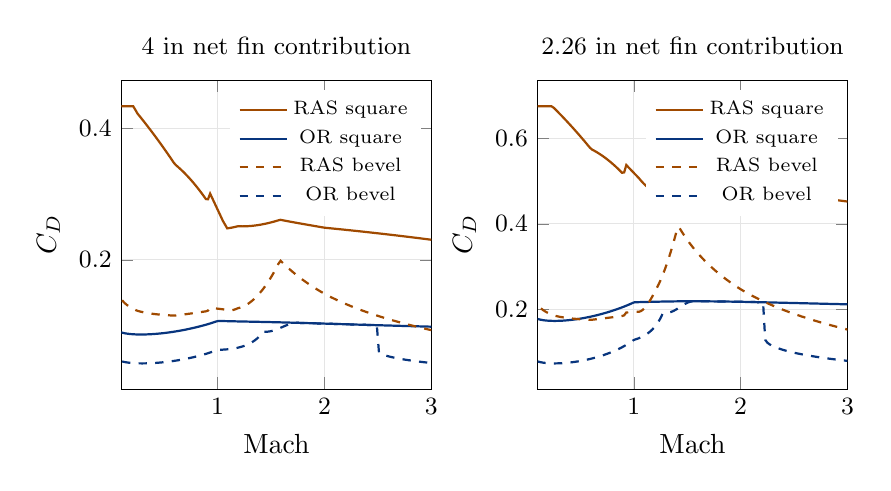
\begin{tikzpicture}
\begin{groupplot}[group style={group size=2 by 1,horizontal sep=1.35cm},width=.455\textwidth,height=5.5cm,xmin=.1,xmax=3,xlabel={Mach},ylabel={$C_D$},grid=major,grid style={gray!20},tick label style={font=\small},title style={font=\small},legend style={font=\scriptsize,draw=none,fill=white,at={(.97,.97)},anchor=north east}]
\nextgroupplot[title={4 in net fin contribution}]
\addplot[thick,burntorange] coordinates {(0.01,0.4332722) (0.03,0.4332722) (0.05,0.4332722) (0.07,0.4332722) (0.09,0.4332722) (0.11,0.4332722) (0.13,0.4332722) (0.15,0.4332722) (0.17,0.4332722) (0.19,0.4332722) (0.21,0.4332722) (0.23,0.4279541) (0.25,0.4222829) (0.27,0.4182894) (0.29,0.4142458) (0.31,0.4101517) (0.33,0.4060075) (0.35,0.4018133) (0.37,0.3975688) (0.39,0.393274) (0.41,0.3889292) (0.43,0.3845341) (0.45,0.3800889) (0.47,0.3755932) (0.49,0.3710477) (0.51,0.3664517) (0.53,0.3618056) (0.55,0.3571095) (0.57,0.3523631) (0.59,0.3475664) (0.61,0.3438513) (0.63,0.3410703) (0.65,0.3381515) (0.67,0.3350951) (0.69,0.3319009) (0.71,0.3285687) (0.73,0.3250988) (0.75,0.3214915) (0.77,0.3177461) (0.79,0.3138631) (0.81,0.3098421) (0.83,0.3056835) (0.85,0.3013871) (0.87,0.2969529) (0.89,0.2923812) (0.91,0.2920159) (0.93,0.3006364) (0.95,0.2937005) (0.97,0.2867645) (0.99,0.2798285) (1.01,0.2728926) (1.03,0.2659566) (1.05,0.2590206) (1.07,0.2533887) (1.09,0.2478347) (1.11,0.2483546) (1.13,0.2488952) (1.15,0.2495405) (1.17,0.2503187) (1.19,0.2510356) (1.21,0.2509212) (1.23,0.2508889) (1.25,0.2509335) (1.27,0.2510508) (1.29,0.2512376) (1.31,0.2514913) (1.33,0.2518095) (1.35,0.2521904) (1.37,0.2526322) (1.39,0.2531334) (1.41,0.2536927) (1.43,0.2543089) (1.45,0.2549808) (1.47,0.2557077) (1.49,0.2564886) (1.51,0.2573229) (1.53,0.2582098) (1.55,0.2591489) (1.57,0.2601397) (1.59,0.2608206) (1.61,0.2601684) (1.63,0.2595312) (1.65,0.2589071) (1.67,0.2582943) (1.69,0.2576913) (1.71,0.2570967) (1.73,0.2565093) (1.75,0.2559278) (1.77,0.2553513) (1.79,0.2547788) (1.81,0.2542095) (1.83,0.2536425) (1.85,0.2530771) (1.87,0.2525128) (1.89,0.2519489) (1.91,0.2513849) (1.93,0.2508204) (1.95,0.2502548) (1.97,0.2496879) (1.99,0.2491193) (2.01,0.2486797) (2.03,0.2483611) (2.05,0.2480413) (2.07,0.2477201) (2.09,0.2473973) (2.11,0.2470728) (2.13,0.2467466) (2.15,0.2464185) (2.17,0.2460885) (2.19,0.2457566) (2.21,0.2454226) (2.23,0.2450867) (2.25,0.2447486) (2.27,0.2444085) (2.29,0.2440664) (2.31,0.2437221) (2.33,0.2433757) (2.35,0.2430273) (2.37,0.2426768) (2.39,0.2423242) (2.41,0.2419695) (2.43,0.2416128) (2.45,0.241254) (2.47,0.2408931) (2.49,0.2405303) (2.51,0.2401653) (2.53,0.2397984) (2.55,0.2394294) (2.57,0.2390584) (2.59,0.2386853) (2.61,0.2383102) (2.63,0.2379331) (2.65,0.2375539) (2.67,0.2371726) (2.69,0.2367892) (2.71,0.2364037) (2.73,0.2360161) (2.75,0.2356262) (2.77,0.2352342) (2.79,0.23484) (2.81,0.2344434) (2.83,0.2340445) (2.85,0.2336433) (2.87,0.2332396) (2.89,0.2328335) (2.91,0.2324248) (2.93,0.2320136) (2.95,0.2315996) (2.97,0.231183) (2.99,0.2307635) (3,0.2305527)};
\addlegendentry{RAS square}
\addplot[thick,B] coordinates {(0.01,0.1068853) (0.03,0.09713073) (0.05,0.09362091) (0.07,0.09160826) (0.09,0.09026025) (0.11,0.08928726) (0.13,0.08855661) (0.15,0.0879972) (0.17,0.08756682) (0.19,0.0872385) (0.21,0.08699402) (0.23,0.08682059) (0.25,0.08670887) (0.27,0.08665188) (0.29,0.08664429) (0.31,0.08668192) (0.33,0.08676146) (0.35,0.08688025) (0.37,0.08703615) (0.39,0.08722736) (0.41,0.08745243) (0.43,0.08771012) (0.45,0.08799942) (0.47,0.08831945) (0.49,0.08866948) (0.51,0.0890489) (0.53,0.08945719) (0.55,0.0898939) (0.57,0.09035865) (0.59,0.09085113) (0.61,0.09137107) (0.63,0.09191827) (0.65,0.09249252) (0.67,0.0930937) (0.69,0.09372169) (0.71,0.0943764) (0.73,0.09505777) (0.75,0.09576576) (0.77,0.09650036) (0.79,0.09726157) (0.81,0.0980494) (0.83,0.0988639) (0.85,0.0997051) (0.87,0.1005731) (0.89,0.1014679) (0.91,0.1024078) (0.93,0.1033961) (0.95,0.1044158) (0.97,0.1054673) (0.99,0.1065511) (1.01,0.1072905) (1.03,0.1071603) (1.05,0.1070576) (1.07,0.1069784) (1.09,0.1069193) (1.11,0.1068473) (1.13,0.1067558) (1.15,0.1066717) (1.17,0.1065933) (1.19,0.1065192) (1.21,0.1064484) (1.23,0.1063797) (1.25,0.1063126) (1.27,0.1062462) (1.29,0.1061801) (1.31,0.1061139) (1.33,0.1060473) (1.35,0.1059799) (1.37,0.1059116) (1.39,0.1058422) (1.41,0.1057716) (1.43,0.1056997) (1.45,0.1056264) (1.47,0.1055517) (1.49,0.1054756) (1.51,0.1053981) (1.53,0.1053193) (1.55,0.105239) (1.57,0.1051574) (1.59,0.1050745) (1.61,0.1049904) (1.63,0.104905) (1.65,0.1048186) (1.67,0.104731) (1.69,0.1046423) (1.71,0.1045527) (1.73,0.1044622) (1.75,0.1043708) (1.77,0.1042786) (1.79,0.1041856) (1.81,0.1040919) (1.83,0.1039976) (1.85,0.1039027) (1.87,0.1038072) (1.89,0.1037113) (1.91,0.1036149) (1.93,0.1035181) (1.95,0.103421) (1.97,0.1033235) (1.99,0.1032258) (2.01,0.1031278) (2.03,0.1030297) (2.05,0.1029314) (2.07,0.102833) (2.09,0.1027345) (2.11,0.1026359) (2.13,0.1025373) (2.15,0.1024388) (2.17,0.1023403) (2.19,0.1022418) (2.21,0.1021435) (2.23,0.1020453) (2.25,0.1019472) (2.27,0.1018492) (2.29,0.1017515) (2.31,0.101654) (2.33,0.1015566) (2.35,0.1014596) (2.37,0.1013628) (2.39,0.1012662) (2.41,0.10117) (2.43,0.101074) (2.45,0.1009784) (2.47,0.1008831) (2.49,0.1007882) (2.51,0.1006936) (2.53,0.1005994) (2.55,0.1005056) (2.57,0.1004121) (2.59,0.1003191) (2.61,0.1002264) (2.63,0.1001342) (2.65,0.1000424) (2.67,0.09995102) (2.69,0.09986007) (2.71,0.09976957) (2.73,0.09967951) (2.75,0.0995899) (2.77,0.09950074) (2.79,0.09941205) (2.81,0.09932382) (2.83,0.09923606) (2.85,0.09914877) (2.87,0.09906195) (2.89,0.09897561) (2.91,0.09888975) (2.93,0.09880437) (2.95,0.09871948) (2.97,0.09863506) (2.99,0.09855114) (3,0.09850936)};
\addlegendentry{OR square}
\addplot[thick,burntorange,dashed] coordinates {(0.01,0.2115638) (0.03,0.1707626) (0.05,0.1562426) (0.07,0.1478541) (0.09,0.1421162) (0.11,0.1378277) (0.13,0.1344416) (0.15,0.1316658) (0.17,0.1293276) (0.19,0.1273168) (0.21,0.1255593) (0.23,0.1240029) (0.25,0.1226097) (0.27,0.1217223) (0.29,0.1209378) (0.31,0.1202403) (0.33,0.1196173) (0.35,0.1190588) (0.37,0.1185564) (0.39,0.1181033) (0.41,0.1176938) (0.43,0.1173231) (0.45,0.116987) (0.47,0.1166822) (0.49,0.1164055) (0.51,0.1161544) (0.53,0.1159265) (0.55,0.1157199) (0.57,0.1155327) (0.59,0.1153635) (0.61,0.1154989) (0.63,0.1159121) (0.65,0.1163332) (0.67,0.1167617) (0.69,0.1171968) (0.71,0.1176381) (0.73,0.1180851) (0.75,0.1185373) (0.77,0.1189944) (0.79,0.119456) (0.81,0.1199217) (0.83,0.1203913) (0.85,0.1208645) (0.87,0.1213411) (0.89,0.1218207) (0.91,0.1228916) (0.93,0.1271565) (0.95,0.1267856) (0.97,0.1264147) (0.99,0.1260438) (1.01,0.1256728) (1.03,0.1253019) (1.05,0.124931) (1.07,0.1243768) (1.09,0.1238298) (1.11,0.1232897) (1.13,0.1233407) (1.15,0.1240542) (1.17,0.1252005) (1.19,0.126569) (1.21,0.1273703) (1.23,0.128506) (1.25,0.129963) (1.27,0.1317324) (1.29,0.133808) (1.31,0.1361856) (1.33,0.1388624) (1.35,0.1418365) (1.37,0.1451068) (1.39,0.148673) (1.41,0.1525351) (1.43,0.1566937) (1.45,0.1611495) (1.47,0.1659038) (1.49,0.1709577) (1.51,0.1763129) (1.53,0.1819711) (1.55,0.1879341) (1.57,0.1942039) (1.59,0.198679) (1.61,0.1954141) (1.63,0.1922669) (1.65,0.1892293) (1.67,0.1862945) (1.69,0.1834558) (1.71,0.1807077) (1.73,0.1780446) (1.75,0.1754619) (1.77,0.1729552) (1.79,0.1705204) (1.81,0.1681538) (1.83,0.165852) (1.85,0.1636119) (1.87,0.1614304) (1.89,0.159305) (1.91,0.157233) (1.93,0.1552121) (1.95,0.1532402) (1.97,0.1513151) (1.99,0.149435) (2.01,0.1476465) (2.03,0.145945) (2.05,0.1442835) (2.07,0.1426604) (2.09,0.1410744) (2.11,0.139524) (2.13,0.138008) (2.15,0.1365253) (2.17,0.1350746) (2.19,0.1336548) (2.21,0.132265) (2.23,0.1309041) (2.25,0.1295711) (2.27,0.1282652) (2.29,0.1269854) (2.31,0.125731) (2.33,0.124501) (2.35,0.1232948) (2.37,0.1221115) (2.39,0.1209505) (2.41,0.119811) (2.43,0.1186924) (2.45,0.1175939) (2.47,0.116515) (2.49,0.1154551) (2.51,0.1144135) (2.53,0.1133896) (2.55,0.112383) (2.57,0.1113929) (2.59,0.110419) (2.61,0.1094606) (2.63,0.1085173) (2.65,0.1075886) (2.67,0.1066739) (2.69,0.1057728) (2.71,0.1048849) (2.73,0.1040096) (2.75,0.1031466) (2.77,0.1022953) (2.79,0.1014554) (2.81,0.1006264) (2.83,0.09980795) (2.85,0.09899958) (2.87,0.09820093) (2.89,0.09741158) (2.91,0.09663115) (2.93,0.09585925) (2.95,0.09509552) (2.97,0.09433958) (2.99,0.09359106) (3,0.09321948)};
\addlegendentry{RAS bevel}
\addplot[thick,B,dashed] coordinates {(0.01,0.06317714) (0.03,0.05342065) (0.05,0.04990699) (0.07,0.0478886) (0.09,0.04653297) (0.11,0.04555048) (0.13,0.04480849) (0.15,0.04423594) (0.17,0.04379064) (0.19,0.04344566) (0.21,0.04318285) (0.23,0.04298946) (0.25,0.04285622) (0.27,0.04277623) (0.29,0.04274422) (0.31,0.04275611) (0.33,0.04280869) (0.35,0.04289941) (0.37,0.04302622) (0.39,0.04318749) (0.41,0.04338188) (0.43,0.04360832) (0.45,0.04386597) (0.47,0.04415414) (0.49,0.04447231) (0.51,0.04482008) (0.53,0.04519718) (0.55,0.04560343) (0.57,0.04603875) (0.59,0.04650314) (0.61,0.04699669) (0.63,0.04751957) (0.65,0.04807202) (0.67,0.04865435) (0.69,0.04926696) (0.71,0.04991033) (0.73,0.05058499) (0.75,0.05129159) (0.77,0.05203084) (0.79,0.05280358) (0.81,0.05361071) (0.83,0.05445327) (0.85,0.05533241) (0.87,0.05624941) (0.89,0.05720573) (0.91,0.05822113) (0.93,0.0593005) (0.95,0.06042888) (0.97,0.06160876) (0.99,0.06284291) (1.01,0.06347643) (1.03,0.06352134) (1.05,0.06364117) (1.07,0.06383896) (1.09,0.06411845) (1.11,0.06445373) (1.13,0.06484578) (1.15,0.06532972) (1.17,0.06591296) (1.19,0.06660438) (1.21,0.06741467) (1.23,0.06835679) (1.25,0.06944649) (1.27,0.07070309) (1.29,0.07215048) (1.31,0.07381861) (1.33,0.07574544) (1.35,0.07797991) (1.37,0.08058632) (1.39,0.08365104) (1.41,0.0872933) (1.43,0.09103184) (1.45,0.09083924) (1.47,0.09097852) (1.49,0.09142118) (1.51,0.09213387) (1.53,0.09307875) (1.55,0.0942138) (1.57,0.09549311) (1.59,0.09686722) (1.61,0.09828335) (1.63,0.09968567) (1.65,0.1010155) (1.67,0.1022116) (1.69,0.1032103) (1.71,0.1039457) (1.73,0.1043498) (1.75,0.1043708) (1.77,0.1042786) (1.79,0.1041856) (1.81,0.1040919) (1.83,0.1039976) (1.85,0.1039027) (1.87,0.1038072) (1.89,0.1037113) (1.91,0.1036149) (1.93,0.1035181) (1.95,0.103421) (1.97,0.1033235) (1.99,0.1032258) (2.01,0.1031278) (2.03,0.1030297) (2.05,0.1029314) (2.07,0.102833) (2.09,0.1027345) (2.11,0.1026359) (2.13,0.1025373) (2.15,0.1024388) (2.17,0.1023403) (2.19,0.1022418) (2.21,0.1021435) (2.23,0.1020453) (2.25,0.1019472) (2.27,0.1018492) (2.29,0.1017515) (2.31,0.101654) (2.33,0.1015566) (2.35,0.1014596) (2.37,0.1013628) (2.39,0.1012662) (2.41,0.10117) (2.43,0.101074) (2.45,0.1009784) (2.47,0.1008831) (2.49,0.1007882) (2.51,0.05930121) (2.53,0.05735013) (2.55,0.0559751) (2.57,0.05485525) (2.59,0.0538893) (2.61,0.05302947) (2.63,0.05224865) (2.65,0.05152969) (2.67,0.05086092) (2.69,0.05023396) (2.71,0.04964258) (2.73,0.04908195) (2.75,0.04854826) (2.77,0.04803845) (2.79,0.04755) (2.81,0.04708082) (2.83,0.04662913) (2.85,0.04619342) (2.87,0.04577239) (2.89,0.04536492) (2.91,0.04497001) (2.93,0.04458679) (2.95,0.04421449) (2.97,0.04385242) (2.99,0.04349996) (3,0.04332716)};
\addlegendentry{OR bevel}
\nextgroupplot[title={2.26 in net fin contribution}]
\addplot[thick,burntorange] coordinates {(0.01,0.6747551) (0.03,0.6747551) (0.05,0.6747551) (0.07,0.6747551) (0.09,0.6747551) (0.11,0.6747551) (0.13,0.6747551) (0.15,0.6747551) (0.17,0.6747551) (0.19,0.6747551) (0.21,0.6747551) (0.23,0.6747551) (0.25,0.6714917) (0.27,0.6665191) (0.29,0.6614791) (0.31,0.6563719) (0.33,0.6511972) (0.35,0.6459552) (0.37,0.6406457) (0.39,0.6352691) (0.41,0.6298249) (0.43,0.6243134) (0.45,0.6187345) (0.47,0.6130884) (0.49,0.6073748) (0.51,0.601594) (0.53,0.5957458) (0.55,0.5898301) (0.57,0.5838472) (0.59,0.5777969) (0.61,0.5735479) (0.63,0.5708768) (0.65,0.568021) (0.67,0.5649802) (0.69,0.5617547) (0.71,0.5583442) (0.73,0.5547487) (0.75,0.5509686) (0.77,0.5470035) (0.79,0.5428537) (0.81,0.5385188) (0.83,0.5339993) (0.85,0.5292945) (0.87,0.5244051) (0.89,0.5193308) (0.91,0.5202382) (0.93,0.5373871) (0.95,0.5321946) (0.97,0.5270021) (0.99,0.5218096) (1.01,0.5166171) (1.03,0.5114247) (1.05,0.5062322) (1.07,0.5002564) (1.09,0.4948707) (1.11,0.49002) (1.13,0.4855619) (1.15,0.4814485) (1.17,0.4776532) (1.19,0.4738938) (1.21,0.4687909) (1.23,0.4639996) (1.25,0.4611105) (1.27,0.4643897) (1.29,0.4678794) (1.31,0.4715752) (1.33,0.4754739) (1.35,0.4795727) (1.37,0.4838694) (1.39,0.4883623) (1.41,0.4930501) (1.43,0.4934108) (1.45,0.4926426) (1.47,0.491929) (1.49,0.491261) (1.51,0.490631) (1.53,0.4900322) (1.55,0.4894587) (1.57,0.4889053) (1.59,0.4883675) (1.61,0.4878414) (1.63,0.4873234) (1.65,0.4868106) (1.67,0.4863001) (1.69,0.4857897) (1.71,0.4852774) (1.73,0.4847612) (1.75,0.4842397) (1.77,0.4837115) (1.79,0.4831754) (1.81,0.4826304) (1.83,0.4820757) (1.85,0.4815105) (1.87,0.4809343) (1.89,0.4803464) (1.91,0.4797466) (1.93,0.4791345) (1.95,0.4785098) (1.97,0.4778723) (1.99,0.4772219) (2.01,0.4767531) (2.03,0.4764546) (2.05,0.4761449) (2.07,0.4758242) (2.09,0.4754927) (2.11,0.4751506) (2.13,0.4747979) (2.15,0.474435) (2.17,0.4740621) (2.19,0.4736794) (2.21,0.4732871) (2.23,0.4728855) (2.25,0.4724748) (2.27,0.4720552) (2.29,0.4716271) (2.31,0.4711905) (2.33,0.4707458) (2.35,0.4702932) (2.37,0.4698329) (2.39,0.4693651) (2.41,0.4688901) (2.43,0.4684079) (2.45,0.4679188) (2.47,0.467423) (2.49,0.4669206) (2.51,0.4664117) (2.53,0.4658966) (2.55,0.4653754) (2.57,0.4648481) (2.59,0.464315) (2.61,0.463776) (2.63,0.4632312) (2.65,0.4626809) (2.67,0.4621249) (2.69,0.4615634) (2.71,0.4609964) (2.73,0.460424) (2.75,0.4598461) (2.77,0.4592627) (2.79,0.458674) (2.81,0.4580798) (2.83,0.4574801) (2.85,0.4568749) (2.87,0.4562642) (2.89,0.4556479) (2.91,0.455026) (2.93,0.4543983) (2.95,0.4537648) (2.97,0.4531255) (2.99,0.4524801) (3,0.4521551)};
\addlegendentry{RAS square}
\addplot[thick,B] coordinates {(0.01,0.2065882) (0.03,0.1901014) (0.05,0.1842085) (0.07,0.1808496) (0.09,0.1786171) (0.11,0.1770223) (0.13,0.1758418) (0.15,0.1749558) (0.17,0.1742934) (0.19,0.1738092) (0.21,0.1734728) (0.23,0.1732625) (0.25,0.1731629) (0.27,0.1731621) (0.29,0.1732514) (0.31,0.1734236) (0.33,0.1736734) (0.35,0.1739963) (0.37,0.1743887) (0.39,0.1748477) (0.41,0.1753709) (0.43,0.1759563) (0.45,0.1766023) (0.47,0.1773073) (0.49,0.1780703) (0.51,0.1788904) (0.53,0.1797666) (0.55,0.1806983) (0.57,0.181685) (0.59,0.1827261) (0.61,0.1838214) (0.63,0.1849705) (0.65,0.1861732) (0.67,0.1874294) (0.69,0.1887389) (0.71,0.1901016) (0.73,0.1915177) (0.75,0.1929871) (0.77,0.1945098) (0.79,0.1960859) (0.81,0.1977157) (0.83,0.1993992) (0.85,0.2011367) (0.87,0.2029283) (0.89,0.2047742) (0.91,0.2067047) (0.93,0.2087249) (0.95,0.2108074) (0.97,0.2129529) (0.99,0.2151622) (1.01,0.2168855) (1.03,0.2169251) (1.05,0.2170126) (1.07,0.2171393) (1.09,0.2172981) (1.11,0.2174335) (1.13,0.2175335) (1.15,0.2176415) (1.17,0.2177542) (1.19,0.2178688) (1.21,0.217983) (1.23,0.2180951) (1.25,0.2182036) (1.27,0.2183074) (1.29,0.2184055) (1.31,0.2184974) (1.33,0.2185825) (1.35,0.2186605) (1.37,0.218731) (1.39,0.2187941) (1.41,0.2188495) (1.43,0.2188973) (1.45,0.2189375) (1.47,0.2189702) (1.49,0.2189957) (1.51,0.2190139) (1.53,0.2190251) (1.55,0.2190295) (1.57,0.2190272) (1.59,0.2190186) (1.61,0.2190038) (1.63,0.218983) (1.65,0.2189565) (1.67,0.2189245) (1.69,0.2188872) (1.71,0.2188449) (1.73,0.2187977) (1.75,0.2187458) (1.77,0.2186896) (1.79,0.2186291) (1.81,0.2185646) (1.83,0.2184962) (1.85,0.2184242) (1.87,0.2183488) (1.89,0.21827) (1.91,0.2181881) (1.93,0.2181033) (1.95,0.2180156) (1.97,0.2179253) (1.99,0.2178325) (2.01,0.2177373) (2.03,0.2176398) (2.05,0.2175403) (2.07,0.2174387) (2.09,0.2173353) (2.11,0.2172301) (2.13,0.2171233) (2.15,0.2170149) (2.17,0.2169051) (2.19,0.2167939) (2.21,0.2166815) (2.23,0.2165679) (2.25,0.2164532) (2.27,0.2163376) (2.29,0.2162209) (2.31,0.2161035) (2.33,0.2159852) (2.35,0.2158662) (2.37,0.2157466) (2.39,0.2156264) (2.41,0.2155056) (2.43,0.2153844) (2.45,0.2152628) (2.47,0.2151407) (2.49,0.2150184) (2.51,0.2148958) (2.53,0.2147729) (2.55,0.2146499) (2.57,0.2145267) (2.59,0.2144034) (2.61,0.21428) (2.63,0.2141566) (2.65,0.2140332) (2.67,0.2139098) (2.69,0.2137864) (2.71,0.2136632) (2.73,0.2135401) (2.75,0.2134171) (2.77,0.2132943) (2.79,0.2131716) (2.81,0.2130492) (2.83,0.212927) (2.85,0.2128051) (2.87,0.2126834) (2.89,0.2125621) (2.91,0.212441) (2.93,0.2123203) (2.95,0.2121999) (2.97,0.2120799) (2.99,0.2119603) (3,0.2119006)};
\addlegendentry{OR square}
\addplot[thick,burntorange,dashed] coordinates {(0.01,0.3115339) (0.03,0.2537606) (0.05,0.2332698) (0.07,0.2214499) (0.09,0.2133729) (0.11,0.2073407) (0.13,0.2025804) (0.15,0.19868) (0.17,0.1953957) (0.19,0.1925723) (0.21,0.1901053) (0.23,0.1879212) (0.25,0.1859666) (0.27,0.1847167) (0.29,0.1836113) (0.31,0.1826283) (0.33,0.1817499) (0.35,0.1809622) (0.37,0.1802532) (0.39,0.1796136) (0.41,0.1790351) (0.43,0.1785112) (0.45,0.1780359) (0.47,0.1776045) (0.49,0.1772126) (0.51,0.1768565) (0.53,0.1765331) (0.55,0.1762395) (0.57,0.1759732) (0.59,0.1757319) (0.61,0.1759134) (0.63,0.1764803) (0.65,0.1770583) (0.67,0.1776465) (0.69,0.1782442) (0.71,0.1788505) (0.73,0.1794648) (0.75,0.1800865) (0.77,0.180715) (0.79,0.1813498) (0.81,0.1819905) (0.83,0.1826366) (0.85,0.1832878) (0.87,0.1839437) (0.89,0.1846039) (0.91,0.1861932) (0.93,0.192865) (0.95,0.1931438) (0.97,0.1934225) (0.99,0.1937012) (1.01,0.1939799) (1.03,0.1942586) (1.05,0.1945374) (1.07,0.1965142) (1.09,0.200405) (1.11,0.2057119) (1.13,0.2122523) (1.15,0.219929) (1.17,0.2286828) (1.19,0.2382113) (1.21,0.2471221) (1.23,0.2570638) (1.25,0.268025) (1.27,0.2799991) (1.29,0.2929826) (1.31,0.3069743) (1.33,0.3219754) (1.35,0.3379884) (1.37,0.3550171) (1.39,0.3730667) (1.41,0.3921429) (1.43,0.3895202) (1.45,0.3813492) (1.47,0.3735942) (1.49,0.3662161) (1.51,0.359181) (1.53,0.3524593) (1.55,0.3460253) (1.57,0.3398562) (1.59,0.333932) (1.61,0.3282348) (1.63,0.3227489) (1.65,0.3174599) (1.67,0.3123551) (1.69,0.307423) (1.71,0.302653) (1.73,0.2980356) (1.75,0.2935622) (1.77,0.289225) (1.79,0.2850165) (1.81,0.2809302) (1.83,0.2769599) (1.85,0.2730999) (1.87,0.269345) (1.89,0.2656902) (1.91,0.2621311) (1.93,0.2586633) (1.95,0.255283) (1.97,0.2519864) (1.99,0.24877) (2.01,0.2456952) (2.03,0.2427547) (2.05,0.2398855) (2.07,0.2370848) (2.09,0.23435) (2.11,0.2316788) (2.13,0.2290688) (2.15,0.226518) (2.17,0.2240241) (2.19,0.2215852) (2.21,0.2191995) (2.23,0.2168651) (2.25,0.2145803) (2.27,0.2123434) (2.29,0.2101529) (2.31,0.2080073) (2.33,0.205905) (2.35,0.2038447) (2.37,0.201825) (2.39,0.1998446) (2.41,0.1979022) (2.43,0.1959967) (2.45,0.1941267) (2.47,0.1922913) (2.49,0.1904891) (2.51,0.1887193) (2.53,0.1869807) (2.55,0.1852723) (2.57,0.1835931) (2.59,0.1819422) (2.61,0.1803185) (2.63,0.1787213) (2.65,0.1771495) (2.67,0.1756024) (2.69,0.174079) (2.71,0.1725785) (2.73,0.1711001) (2.75,0.1696429) (2.77,0.1682063) (2.79,0.1667894) (2.81,0.1653915) (2.83,0.1640118) (2.85,0.1626495) (2.87,0.1613041) (2.89,0.1599746) (2.91,0.1586606) (2.93,0.1573612) (2.95,0.1560758) (2.97,0.1548037) (2.99,0.1535443) (3,0.1529192)};
\addlegendentry{RAS bevel}
\addplot[thick,B,dashed] coordinates {(0.01,0.1072643) (0.03,0.09077713) (0.05,0.08488356) (0.07,0.08152361) (0.09,0.07928985) (0.11,0.07769373) (0.13,0.07651183) (0.15,0.07562462) (0.17,0.07496129) (0.19,0.07447672) (0.21,0.07414061) (0.23,0.07393172) (0.25,0.07383473) (0.27,0.0738383) (0.29,0.07393387) (0.31,0.07411488) (0.33,0.0743763) (0.35,0.07471421) (0.37,0.07512559) (0.39,0.07560812) (0.41,0.07616005) (0.43,0.07678013) (0.45,0.07746749) (0.47,0.07822162) (0.49,0.07904234) (0.51,0.07992973) (0.53,0.08088416) (0.55,0.08190622) (0.57,0.08299679) (0.59,0.08415694) (0.61,0.08538805) (0.63,0.08669169) (0.65,0.08806974) (0.67,0.08952435) (0.69,0.09105797) (0.71,0.09267337) (0.73,0.09437371) (0.75,0.09616253) (0.77,0.09804381) (0.79,0.100022) (0.81,0.1021023) (0.83,0.1042903) (0.85,0.1065925) (0.87,0.1090161) (0.89,0.1115696) (0.91,0.1142922) (0.93,0.1171997) (0.95,0.120277) (0.97,0.1235388) (0.99,0.1270022) (1.01,0.1294983) (1.03,0.1310661) (1.05,0.1329254) (1.07,0.1351074) (1.09,0.13765) (1.11,0.1405502) (1.13,0.1438595) (1.15,0.147699) (1.17,0.1521632) (1.19,0.1573754) (1.21,0.1634996) (1.23,0.1707602) (1.25,0.1794725) (1.27,0.1900968) (1.29,0.1914448) (1.31,0.1916295) (1.33,0.1925476) (1.35,0.1941271) (1.37,0.1962776) (1.39,0.1988922) (1.41,0.2018478) (1.43,0.2050072) (1.45,0.2082195) (1.47,0.2113216) (1.49,0.2141389) (1.51,0.2164865) (1.53,0.2181698) (1.55,0.2189853) (1.57,0.2190272) (1.59,0.2190186) (1.61,0.2190038) (1.63,0.218983) (1.65,0.2189565) (1.67,0.2189245) (1.69,0.2188872) (1.71,0.2188449) (1.73,0.2187977) (1.75,0.2187458) (1.77,0.2186896) (1.79,0.2186291) (1.81,0.2185646) (1.83,0.2184962) (1.85,0.2184242) (1.87,0.2183488) (1.89,0.21827) (1.91,0.2181881) (1.93,0.2181033) (1.95,0.2180156) (1.97,0.2179253) (1.99,0.2178325) (2.01,0.2177373) (2.03,0.2176398) (2.05,0.2175403) (2.07,0.2174387) (2.09,0.2173353) (2.11,0.2172301) (2.13,0.2171233) (2.15,0.2170149) (2.17,0.2169051) (2.19,0.2167939) (2.21,0.2166815) (2.23,0.1289988) (2.25,0.1222238) (2.27,0.1185032) (2.29,0.1156399) (2.31,0.1132394) (2.33,0.1111408) (2.35,0.1092596) (2.37,0.1075448) (2.39,0.1059626) (2.41,0.1044896) (2.43,0.1031084) (2.45,0.1018059) (2.47,0.1005718) (2.49,0.0993981) (2.51,0.09827797) (2.53,0.09720596) (2.55,0.09617743) (2.57,0.09518847) (2.59,0.09423572) (2.61,0.09331627) (2.63,0.09242758) (2.65,0.09156744) (2.67,0.09073387) (2.69,0.08992511) (2.71,0.08913961) (2.73,0.08837596) (2.75,0.08763288) (2.77,0.08690923) (2.79,0.08620396) (2.81,0.0855161) (2.83,0.0848448) (2.85,0.08418923) (2.87,0.08354866) (2.89,0.0829224) (2.91,0.08230982) (2.93,0.08171032) (2.95,0.08112337) (2.97,0.08054844) (2.99,0.07998506) (3,0.07970757)};
\addlegendentry{OR bevel}
\end{groupplot}\end{tikzpicture}
\caption{Paired subtraction isolates the net effect of adding fins, including any fin/body interaction. RASAero does not expose a pressure/friction split; these are not isolated fin-pressure coefficients.}\end{figure}


Fin-count scaling agrees in both programs: replacing four H fins with three changes the RASAero net contribution by the expected factor 0.75, with a maximum coefficient residual below $1.6\times10^{-7}$ over the full sweep. A fin-count convention error does not explain the gap.



\clearpage\subsection{Tangent-ogive nose pressure: the strongest corrective lead}
The installed MIT engine returns only $C_{D,\mathrm{nose}}=0.000474$ for the H tangent ogive at Mach 2. Source inspection identifies the geometric input used in \code{SymmetricComponentCalc}: the slope is estimated over the last one percent of nose length,
\begin{equation}
 s_{\mathrm{tail}}=\frac{R-r(0.99L_n)}{\sqrt{[R-r(0.99L_n)]^2+(0.01L_n)^2}}.
\end{equation}
That value approaches zero for a nose tangent to its cylindrical body. The ogive branch then feeds it into a cone-like supersonic pressure formula. The H value is approximately 0.001622, whereas the radius/length equivalent-cone sine is 0.164399. This explains the near-zero pressure term and its very weak sensitivity to nose fineness. At Mach 2, shortening the H nose from 12 to 6 in raises RASAero body $C_D$ from 0.33796 to 0.60324; OR changes only from 0.21948 to 0.22346.

\textbf{Offline trial, with no fitted constants.} As a diagnostic, retain OR friction and base drag, replace only the ogive pressure term, and evaluate the existing supersonic functional form using the overall cone angle:
\begin{align}
 s_*&=\frac{R}{\sqrt{L_n^2+R^2}},\\
 \widehat C_{D,n}&=2.1s_*^2+\frac{0.5s_*}{\sqrt{M^2-1}},\quad M\geq1.32,\\
 \widehat C_D&=C_{D,\mathrm{OR}}-C_{D,n,\mathrm{OR}}+\widehat C_{D,n}.
\end{align}
This is a post-processing hypothesis, not an installed patch or an experimentally validated ogive model. It does not use a RASAero coefficient in its calculation. No claim is made for its extension through Mach 1.

\begin{table}[H]\centering\small\renewcommand{\arraystretch}{1.12}
\caption{Nose-only trial on six finless geometries, 169 Mach points each, 1.32--3.00. MAPE uses RASAero as denominator.}\label{tab:nosetrial}
\begin{tabular}{@{}lrrrr@{}}\toprule
 & \multicolumn{2}{c}{Mean absolute $C_D$ error} & \multicolumn{2}{c}{Mean absolute error [\%]}\\
Geometry & Original & Trial & Original & Trial\\\midrule


H & 0.11616 & 0.01571 & 35.71 & 5.03\\

S & 0.06672 & 0.00924 & 20.70 & 2.99\\

H-short & 0.11543 & 0.01596 & 39.73 & 5.69\\

H-long & 0.11730 & 0.01536 & 30.10 & 4.13\\

H-nose6 & 0.37479 & 0.07304 & 63.63 & 12.66\\

H-nose18 & 0.06422 & 0.00919 & 23.75 & 3.52\\


\bottomrule\end{tabular}\end{table}
The aggregate mean absolute coefficient error falls from 0.14244 to 0.02308 (83.8\%). The stubby 6 in nose still has 12.66\% mean error, so this simple trial is not a general replacement model. A dedicated tangent/secant-ogive wave-drag treatment, with a separately validated transonic join, is the preferred improvement.


\clearpage

\begin{figure}[H]\centering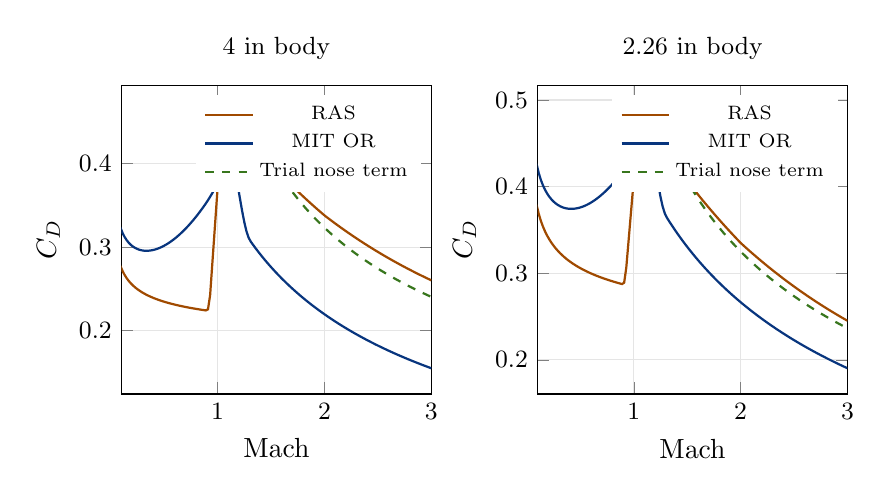
\begin{tikzpicture}
\begin{groupplot}[group style={group size=2 by 1,horizontal sep=1.35cm},width=.455\textwidth,height=5.5cm,xmin=.1,xmax=3,xlabel={Mach},ylabel={$C_D$},grid=major,grid style={gray!20},tick label style={font=\small},title style={font=\small},legend style={font=\scriptsize,draw=none,fill=white,at={(.97,.97)},anchor=north east}]
\nextgroupplot[title={4 in body}]
\addplot[thick,burntorange] coordinates {(0.01,0.3747526) (0.03,0.3184175) (0.05,0.2978187) (0.07,0.2858134) (0.09,0.2775679) (0.11,0.2713925) (0.13,0.2665116) (0.15,0.2625091) (0.17,0.2591377) (0.19,0.2562395) (0.21,0.2537077) (0.23,0.251467) (0.25,0.2494629) (0.27,0.247654) (0.29,0.246009) (0.31,0.2445031) (0.33,0.2431167) (0.35,0.2418338) (0.37,0.2406415) (0.39,0.2395289) (0.41,0.238487) (0.43,0.2375083) (0.45,0.2365861) (0.47,0.235715) (0.49,0.2348901) (0.51,0.2341071) (0.53,0.2333626) (0.55,0.2326532) (0.57,0.2319761) (0.59,0.2313287) (0.61,0.2307088) (0.63,0.2301145) (0.65,0.2295438) (0.67,0.2289953) (0.69,0.2284673) (0.71,0.2279585) (0.73,0.2274678) (0.75,0.2269941) (0.77,0.2265363) (0.79,0.2260934) (0.81,0.2256647) (0.83,0.2252494) (0.85,0.2248467) (0.87,0.224456) (0.89,0.2240767) (0.91,0.2254135) (0.93,0.2425879) (0.95,0.2793136) (0.97,0.3160393) (0.99,0.352765) (1.01,0.3894907) (1.03,0.4262165) (1.05,0.4629422) (1.07,0.4610516) (1.09,0.4592147) (1.11,0.4574285) (1.13,0.4556897) (1.15,0.4539954) (1.17,0.4505311) (1.19,0.4470889) (1.21,0.4436996) (1.23,0.4403608) (1.25,0.4370707) (1.27,0.4338274) (1.29,0.4306293) (1.31,0.4274746) (1.33,0.4243618) (1.35,0.4212897) (1.37,0.4182567) (1.39,0.415262) (1.41,0.412304) (1.43,0.4093818) (1.45,0.4064945) (1.47,0.4036408) (1.49,0.4008202) (1.51,0.3980314) (1.53,0.3952739) (1.55,0.3925467) (1.57,0.3898493) (1.59,0.3871808) (1.61,0.3845406) (1.63,0.3819281) (1.65,0.3793426) (1.67,0.3767835) (1.69,0.3742506) (1.71,0.371743) (1.73,0.3692601) (1.75,0.3668018) (1.77,0.3643675) (1.79,0.3619566) (1.81,0.3595688) (1.83,0.3572039) (1.85,0.354861) (1.87,0.3525402) (1.89,0.3502408) (1.91,0.3479626) (1.93,0.3457054) (1.95,0.3434686) (1.97,0.341252) (1.99,0.3390554) (2.01,0.336981) (2.03,0.3350224) (2.05,0.3330831) (2.07,0.3311632) (2.09,0.3292624) (2.11,0.3273803) (2.13,0.325517) (2.15,0.323672) (2.17,0.3218454) (2.19,0.3200369) (2.21,0.3182462) (2.23,0.3164733) (2.25,0.314718) (2.27,0.31298) (2.29,0.3112593) (2.31,0.3095557) (2.33,0.307869) (2.35,0.3061989) (2.37,0.3045456) (2.39,0.3029086) (2.41,0.3012879) (2.43,0.2996833) (2.45,0.2980948) (2.47,0.2965221) (2.49,0.2949651) (2.51,0.2934237) (2.53,0.2918976) (2.55,0.2903869) (2.57,0.2888913) (2.59,0.2874107) (2.61,0.2859449) (2.63,0.284494) (2.65,0.2830576) (2.67,0.2816356) (2.69,0.2802281) (2.71,0.2788348) (2.73,0.2774556) (2.75,0.2760903) (2.77,0.2747388) (2.79,0.273401) (2.81,0.2720768) (2.83,0.2707662) (2.85,0.2694688) (2.87,0.2681846) (2.89,0.2669135) (2.91,0.2656555) (2.93,0.2644102) (2.95,0.2631777) (2.97,0.2619578) (2.99,0.2607504) (3,0.2601514)};
\addlegendentry{RAS}
\addplot[thick,B] coordinates {(0.01,0.432385) (0.03,0.368739) (0.05,0.3457716) (0.07,0.3325257) (0.09,0.3235729) (0.11,0.3170244) (0.13,0.312015) (0.15,0.308081) (0.17,0.3049468) (0.19,0.3024363) (0.21,0.3004307) (0.23,0.2988461) (0.25,0.2976214) (0.27,0.2967108) (0.29,0.2960791) (0.31,0.2956987) (0.33,0.2955475) (0.35,0.295608) (0.37,0.2958654) (0.39,0.2963078) (0.41,0.296925) (0.43,0.2977085) (0.45,0.298651) (0.47,0.2997464) (0.49,0.3009891) (0.51,0.3023746) (0.53,0.3038987) (0.55,0.3055578) (0.57,0.3073487) (0.59,0.3092686) (0.61,0.311315) (0.63,0.3134857) (0.65,0.3157785) (0.67,0.3181918) (0.69,0.3207238) (0.71,0.3233731) (0.73,0.3261383) (0.75,0.3290182) (0.77,0.3320116) (0.79,0.3351176) (0.81,0.3383351) (0.83,0.3416633) (0.85,0.3451015) (0.87,0.3486487) (0.89,0.3523045) (0.91,0.3561867) (0.93,0.3603149) (0.95,0.3645779) (0.97,0.368977) (0.99,0.3735132) (1.01,0.3876035) (1.03,0.4073131) (1.05,0.4196834) (1.07,0.4255951) (1.09,0.4259297) (1.11,0.4213711) (1.13,0.4127735) (1.15,0.4012075) (1.17,0.3875552) (1.19,0.3726995) (1.21,0.3575234) (1.23,0.3429105) (1.25,0.3297446) (1.27,0.3189102) (1.29,0.3112917) (1.31,0.3065889) (1.33,0.3030196) (1.35,0.2995423) (1.37,0.296153) (1.39,0.2928476) (1.41,0.2896227) (1.43,0.2864748) (1.45,0.2834006) (1.47,0.2803974) (1.49,0.2774621) (1.51,0.2745922) (1.53,0.2717851) (1.55,0.2690386) (1.57,0.2663503) (1.59,0.2637182) (1.61,0.2611402) (1.63,0.2586144) (1.65,0.2561391) (1.67,0.2537124) (1.69,0.2513329) (1.71,0.2489988) (1.73,0.2467089) (1.75,0.2444615) (1.77,0.2422554) (1.79,0.2400894) (1.81,0.2379621) (1.83,0.2358724) (1.85,0.2338192) (1.87,0.2318014) (1.89,0.2298179) (1.91,0.2278679) (1.93,0.2259504) (1.95,0.2240644) (1.97,0.222209) (1.99,0.2203836) (2.01,0.2185872) (2.03,0.2168191) (2.05,0.2150786) (2.07,0.2133649) (2.09,0.2116774) (2.11,0.2100153) (2.13,0.2083782) (2.15,0.2067653) (2.17,0.2051761) (2.19,0.2036101) (2.21,0.2020666) (2.23,0.2005451) (2.25,0.1990452) (2.27,0.1975663) (2.29,0.196108) (2.31,0.1946698) (2.33,0.1932513) (2.35,0.191852) (2.37,0.1904715) (2.39,0.1891094) (2.41,0.1877654) (2.43,0.186439) (2.45,0.1851299) (2.47,0.1838377) (2.49,0.1825621) (2.51,0.1813028) (2.53,0.1800594) (2.55,0.1788316) (2.57,0.1776191) (2.59,0.1764217) (2.61,0.175239) (2.63,0.1740707) (2.65,0.1729166) (2.67,0.1717764) (2.69,0.1706498) (2.71,0.1695367) (2.73,0.1684367) (2.75,0.1673496) (2.77,0.1662753) (2.79,0.1652134) (2.81,0.1641637) (2.83,0.1631261) (2.85,0.1621003) (2.87,0.1610861) (2.89,0.1600834) (2.91,0.1590919) (2.93,0.1581114) (2.95,0.1571418) (2.97,0.1561828) (2.99,0.1552344) (3,0.154764)};
\addlegendentry{MIT OR}
\addplot[thick,g,dashed] coordinates {(1.33,0.4525878) (1.35,0.4460353) (1.37,0.4398178) (1.39,0.4338996) (1.41,0.428251) (1.43,0.4228466) (1.45,0.4176647) (1.47,0.4126866) (1.49,0.407896) (1.51,0.4032786) (1.53,0.3988218) (1.55,0.3945144) (1.57,0.3903464) (1.59,0.3863091) (1.61,0.3823942) (1.63,0.3785945) (1.65,0.3749035) (1.67,0.3713151) (1.69,0.3678238) (1.71,0.3644246) (1.73,0.361113) (1.75,0.3578845) (1.77,0.3547353) (1.79,0.3516617) (1.81,0.3486604) (1.83,0.3457281) (1.85,0.342862) (1.87,0.3400592) (1.89,0.3373173) (1.91,0.3346337) (1.93,0.3320063) (1.95,0.3294329) (1.97,0.3269115) (1.99,0.3244402) (2.01,0.3220173) (2.03,0.3196409) (2.05,0.3173097) (2.07,0.3150219) (2.09,0.3127763) (2.11,0.3105714) (2.13,0.308406) (2.15,0.3062787) (2.17,0.3041885) (2.19,0.3021343) (2.21,0.3001148) (2.23,0.2981292) (2.25,0.2961765) (2.27,0.2942557) (2.29,0.292366) (2.31,0.2905064) (2.33,0.2886762) (2.35,0.2868746) (2.37,0.2851008) (2.39,0.2833542) (2.41,0.281634) (2.43,0.2799395) (2.45,0.2782701) (2.47,0.2766253) (2.49,0.2750043) (2.51,0.2734067) (2.53,0.2718318) (2.55,0.2702792) (2.57,0.2687483) (2.59,0.2672387) (2.61,0.2657498) (2.63,0.2642812) (2.65,0.2628325) (2.67,0.2614031) (2.69,0.2599928) (2.71,0.258601) (2.73,0.2572275) (2.75,0.2558718) (2.77,0.2545335) (2.79,0.2532123) (2.81,0.2519079) (2.83,0.2506198) (2.85,0.2493479) (2.87,0.2480917) (2.89,0.246851) (2.91,0.2456254) (2.93,0.2444148) (2.95,0.2432187) (2.97,0.2420369) (2.99,0.2408692) (3,0.2402905)};
\addlegendentry{Trial nose term}
\nextgroupplot[title={2.26 in body}]
\addplot[thick,burntorange] coordinates {(0.01,0.5386952) (0.03,0.4468266) (0.05,0.412889) (0.07,0.3929775) (0.09,0.3792307) (0.11,0.3688906) (0.13,0.3606872) (0.15,0.3539377) (0.17,0.3482354) (0.19,0.3433197) (0.21,0.3390145) (0.23,0.3351955) (0.25,0.3317718) (0.27,0.3286753) (0.29,0.3258536) (0.31,0.3232657) (0.33,0.3208787) (0.35,0.3186662) (0.37,0.3166065) (0.39,0.3146814) (0.41,0.312876) (0.43,0.3111773) (0.45,0.3095747) (0.47,0.3080585) (0.49,0.3066209) (0.51,0.3052547) (0.53,0.3039538) (0.55,0.3027128) (0.57,0.3015268) (0.59,0.3003916) (0.61,0.2993034) (0.63,0.2982588) (0.65,0.2972547) (0.67,0.2962885) (0.69,0.2953575) (0.71,0.2944596) (0.73,0.2935926) (0.75,0.2927547) (0.77,0.2919442) (0.79,0.2911595) (0.81,0.2903992) (0.83,0.2896619) (0.85,0.2889464) (0.87,0.2882516) (0.89,0.2875763) (0.91,0.289199) (0.93,0.3067123) (0.95,0.3357469) (0.97,0.3647815) (0.99,0.3938161) (1.01,0.4228506) (1.03,0.4518852) (1.05,0.4809198) (1.07,0.4785135) (1.09,0.4761658) (1.11,0.4738733) (1.13,0.4716328) (1.15,0.4694413) (1.17,0.465484) (1.19,0.461553) (1.21,0.4576787) (1.23,0.4538589) (1.25,0.4500916) (1.27,0.4463747) (1.29,0.4427065) (1.31,0.4390853) (1.33,0.4355094) (1.35,0.4319773) (1.37,0.4284877) (1.39,0.4250393) (1.41,0.4216307) (1.43,0.4182609) (1.45,0.4149287) (1.47,0.4116331) (1.49,0.4083732) (1.51,0.4051478) (1.53,0.4019563) (1.55,0.3987977) (1.57,0.3956712) (1.59,0.3925762) (1.61,0.3895118) (1.63,0.3864774) (1.65,0.3834722) (1.67,0.3804958) (1.69,0.3775476) (1.71,0.3746268) (1.73,0.3717329) (1.75,0.3688656) (1.77,0.3660242) (1.79,0.3632082) (1.81,0.3604172) (1.83,0.3576509) (1.85,0.3549085) (1.87,0.3521899) (1.89,0.3494946) (1.91,0.3468222) (1.93,0.3441724) (1.95,0.3415447) (1.97,0.3389388) (1.99,0.3363545) (2.01,0.3339467) (2.03,0.3317054) (2.05,0.3294853) (2.07,0.3272863) (2.09,0.325108) (2.11,0.3229502) (2.13,0.320813) (2.15,0.3186959) (2.17,0.3165987) (2.19,0.3145216) (2.21,0.3124639) (2.23,0.3104258) (2.25,0.308407) (2.27,0.3064073) (2.29,0.3044266) (2.31,0.3024646) (2.33,0.3005214) (2.35,0.2985965) (2.37,0.2966901) (2.39,0.2948018) (2.41,0.2929315) (2.43,0.291079) (2.45,0.2892444) (2.47,0.2874272) (2.49,0.2856274) (2.51,0.283845) (2.53,0.2820796) (2.55,0.2803312) (2.57,0.2785996) (2.59,0.2768848) (2.61,0.2751864) (2.63,0.2735045) (2.65,0.2718389) (2.67,0.2701893) (2.69,0.2685559) (2.71,0.2669382) (2.73,0.2653363) (2.75,0.26375) (2.77,0.2621791) (2.79,0.2606235) (2.81,0.2590831) (2.83,0.2575579) (2.85,0.2560475) (2.87,0.2545519) (2.89,0.253071) (2.91,0.2516046) (2.93,0.2501526) (2.95,0.2487149) (2.97,0.2472914) (2.99,0.2458819) (3,0.2451824)};
\addlegendentry{RAS}
\addplot[thick,B] coordinates {(0.01,0.5954135) (0.03,0.4965406) (0.05,0.4609371) (0.07,0.4403442) (0.09,0.426335) (0.11,0.4159831) (0.13,0.40795) (0.15,0.4015189) (0.17,0.3962643) (0.19,0.3919144) (0.21,0.3882857) (0.23,0.3852492) (0.25,0.3827105) (0.27,0.3805991) (0.29,0.3788608) (0.31,0.3774531) (0.33,0.3763422) (0.35,0.3755008) (0.37,0.3749065) (0.39,0.3745408) (0.41,0.374388) (0.43,0.3744352) (0.45,0.374671) (0.47,0.375086) (0.49,0.3756719) (0.51,0.3764214) (0.53,0.3773283) (0.55,0.378387) (0.57,0.3795927) (0.59,0.3809409) (0.61,0.3824279) (0.63,0.3840502) (0.65,0.3858047) (0.67,0.3876885) (0.69,0.3896993) (0.71,0.3918346) (0.73,0.3940924) (0.75,0.3964708) (0.77,0.3989682) (0.79,0.4015828) (0.81,0.4043133) (0.83,0.4071583) (0.85,0.4101167) (0.87,0.4131872) (0.89,0.4163687) (0.91,0.419839) (0.93,0.4236273) (0.95,0.4275664) (0.97,0.4316579) (0.99,0.4359037) (1.01,0.4497257) (1.03,0.4691906) (1.05,0.4813365) (1.07,0.4870446) (1.09,0.487197) (1.11,0.4823783) (1.13,0.4734285) (1.15,0.4615137) (1.17,0.4475156) (1.19,0.4323167) (1.21,0.4168) (1.23,0.4018486) (1.25,0.3883464) (1.27,0.3771772) (1.29,0.3692257) (1.31,0.3641911) (1.33,0.3602913) (1.35,0.3564849) (1.37,0.3527679) (1.39,0.3491364) (1.41,0.3455869) (1.43,0.342116) (1.45,0.3387205) (1.47,0.3353976) (1.49,0.3321443) (1.51,0.3289581) (1.53,0.3258365) (1.55,0.3227771) (1.57,0.3197777) (1.59,0.3168361) (1.61,0.3139505) (1.63,0.3111188) (1.65,0.3083394) (1.67,0.3056104) (1.69,0.3029302) (1.71,0.3002973) (1.73,0.2977102) (1.75,0.2951675) (1.77,0.2926679) (1.79,0.29021) (1.81,0.2877927) (1.83,0.2854147) (1.85,0.283075) (1.87,0.2807725) (1.89,0.2785061) (1.91,0.2762748) (1.93,0.2740778) (1.95,0.2719141) (1.97,0.2697829) (1.99,0.2676833) (2.01,0.2656145) (2.03,0.2635757) (2.05,0.2615662) (2.07,0.2595854) (2.09,0.2576324) (2.11,0.2557067) (2.13,0.2538076) (2.15,0.2519345) (2.17,0.2500869) (2.19,0.248264) (2.21,0.2464655) (2.23,0.2446907) (2.25,0.2429392) (2.27,0.2412104) (2.29,0.2395039) (2.31,0.2378192) (2.33,0.2361558) (2.35,0.2345134) (2.37,0.2328915) (2.39,0.2312896) (2.41,0.2297075) (2.43,0.2281447) (2.45,0.2266008) (2.47,0.2250755) (2.49,0.2235684) (2.51,0.2220792) (2.53,0.2206076) (2.55,0.2191532) (2.57,0.2177158) (2.59,0.2162949) (2.61,0.2148904) (2.63,0.2135019) (2.65,0.2121292) (2.67,0.210772) (2.69,0.20943) (2.71,0.2081029) (2.73,0.2067906) (2.75,0.2054927) (2.77,0.204209) (2.79,0.2029394) (2.81,0.2016835) (2.83,0.2004411) (2.85,0.1992121) (2.87,0.1979961) (2.89,0.1967931) (2.91,0.1956028) (2.93,0.194425) (2.95,0.1932595) (2.97,0.1921061) (2.99,0.1909647) (3,0.1903984)};
\addlegendentry{MIT OR}
\addplot[thick,g,dashed] coordinates {(1.33,0.4501553) (1.35,0.4442487) (1.37,0.4386002) (1.39,0.4331843) (1.41,0.4279795) (1.43,0.4229675) (1.45,0.4181325) (1.47,0.4134609) (1.49,0.4089405) (1.51,0.4045608) (1.53,0.4003125) (1.55,0.3961871) (1.57,0.3921771) (1.59,0.3882759) (1.61,0.3844772) (1.63,0.3807755) (1.65,0.3771658) (1.67,0.3736433) (1.69,0.3702039) (1.71,0.3668436) (1.73,0.3635587) (1.75,0.360346) (1.77,0.3572023) (1.79,0.3541246) (1.81,0.3511103) (1.83,0.3481569) (1.85,0.345262) (1.87,0.3424234) (1.89,0.339639) (1.91,0.3369068) (1.93,0.3342249) (1.95,0.3315918) (1.97,0.3290056) (1.99,0.3264649) (2.01,0.3239682) (2.03,0.321514) (2.05,0.3191012) (2.07,0.3167282) (2.09,0.3143941) (2.11,0.3120977) (2.13,0.3098378) (2.15,0.3076134) (2.17,0.3054235) (2.19,0.3032673) (2.21,0.3011437) (2.23,0.2990519) (2.25,0.2969912) (2.27,0.2949606) (2.29,0.2929594) (2.31,0.2909869) (2.33,0.2890424) (2.35,0.2871253) (2.37,0.2852347) (2.39,0.2833703) (2.41,0.2815312) (2.43,0.279717) (2.45,0.2779271) (2.47,0.2761609) (2.49,0.2744179) (2.51,0.2726977) (2.53,0.2709997) (2.55,0.2693235) (2.57,0.2676686) (2.59,0.2660345) (2.61,0.2644209) (2.63,0.2628273) (2.65,0.2612534) (2.67,0.2596987) (2.69,0.2581629) (2.71,0.2566455) (2.73,0.2551463) (2.75,0.253665) (2.77,0.2522011) (2.79,0.2507543) (2.81,0.2493244) (2.83,0.2479111) (2.85,0.2465139) (2.87,0.2451327) (2.89,0.2437672) (2.91,0.242417) (2.93,0.241082) (2.95,0.2397618) (2.97,0.2384562) (2.99,0.237165) (3,0.2365248)};
\addlegendentry{Trial nose term}
\end{groupplot}\end{tikzpicture}
\caption{An offline, unfitted nose-term substitution substantially closes the supersonic finless-body gap. The trial is defined only from Mach 1.32 upward and leaves original OR friction and base drag intact.}\end{figure}


\subsection{Fin profile, thickness and sweep}
The square-to-beveled change provides a strong profile diagnostic at identical planform and fin count. At Mach 0.3, the H total-coefficient reduction is 0.29163 in RASAero versus 0.04391 in OR, a factor of 6.64. At Mach 2, OR gives the same $C_D=0.32266$ for Hsq and Hbev, while RASAero gives 0.58680 and 0.48648 respectively. Body drag cancels in these comparisons.

In \code{FinSetCalc}, the MIT triangular branch uses leading-edge-normal Mach, a weak attached wedge-shock calculation, and a fallback to the square-edge stagnation coefficient when no attached solution is found. That fallback produces identical square/bevel fin pressure coefficients over Mach 1.75--2.49 for H and 1.56--2.22 for S in this sweep. This loss of profile sensitivity is an implementation mechanism, not a mismatched RASAero airfoil selection. Even doubling H bevel length from 0.25 to 0.50 in leaves the OR total unchanged at Mach 2 (0.32266), while RASAero decreases from 0.48648 to 0.44915.

\textbf{Proposed direction.} Replace the all-or-nothing detached-shock fallback with a finite-thickness fin model that retains section geometry in attached, detached and transonic regimes. Check the coordinate projection consistently: with chordwise bevel distance $b$ and leading-edge sweep $\Lambda$, the normal-section distance is $b\cos\Lambda$, so the normal wedge angle is $\tan^{-1}[t/(2b\cos\Lambda)]$. The present source uses the chordwise angle with normal Mach. This is a geometric consistency item to investigate, not a tested standalone correction. A normal-section wedge alone also does not account for the complete finite fin and its expansion/base regions.

Use independent sweep/profile fixtures as acceptance cases. At Mach 0.8, removing H square-fin sweep increases total $C_D$ by 0.03781 in RASAero and 0.07748 in OR. For H beveled fins the increases are 0.01027 and 0.06198. Increasing one constant drag multiplier would not reproduce both responses.



\clearpage\subsection{Friction, base drag and limits of matching RASAero}
\textbf{Fin-local Reynolds number is supported by a length-invariance test.} OR computes one turbulent skin-friction coefficient from the entire aerodynamic rocket length and applies it to the fins. Lengthening the H body from 48 to 96 in leaves the RASAero net square-fin addition unchanged at Mach 0.3 (0.41220), while OR decreases it from 0.08666 to 0.08446. Evaluating the same OR correlation on fin mean aerodynamic chord removes that artificial body-length dependence in this isolated smooth-fin model.

The candidate uses $Re_f=V\bar c/\nu$ in the existing fin wetted-area expression,
\begin{equation}
 C_{D,f,\mathrm{friction}}=C_f(Re_f,M)\left(1+\frac{2t}{\bar c}\right)\frac{2NS_f}{A_{\mathrm{ref}}}.
\end{equation}
At Mach 0.3 it adds only 0.01515 (H) or 0.02504 (S) to OR $C_D$, compared with square-fin contribution gaps of 0.32555 and 0.48560. Thus it is a targeted structural improvement, not an explanation of the full discrepancy. Root boundary-layer interaction and roughness should be treated explicitly rather than inferred from a universal friction factor.

\textbf{Base-drag treatment needs a separate audit.} OR's body base term is $0.12+0.13M^2$ below Mach 1 and $0.25/M$ above it. The nearly common H/S subsonic body residual suggests a Mach-dependent body/base contribution rather than an overall geometry scale error. Changing the RASAero diagnostic nozzle diameter from zero to the full body diameter leaves power-off $C_D$ unchanged and produces the same power-off/on difference for H and S:
\begin{table}[H]\centering\small
\caption{Nozzle-sensitive drag contribution compared with OR's full body-base term. The two columns are different observables, not an asserted component identity.}
\begin{tabular}{@{}rrr@{}}\toprule
Mach & RAS full-nozzle $C_{D,off}-C_{D,on}$ & OR body-base $C_D$\\\midrule
0.30 & 0.05470 & 0.13170\\
0.80 & 0.07919 & 0.20320\\
1.00 & 0.13208 & 0.25000\\
1.20 & 0.14780 & 0.20833\\
2.00 & 0.14894 & 0.12500\\
3.00 & 0.12360 & 0.08333\\\bottomrule
\end{tabular}\end{table}
The export does not establish that a full nozzle removes every base-pressure effect, so the difference is not used as an absolute RASAero base coefficient. A future model should separate body base drag, fin trailing-edge drag and powered nozzle/plume effects; simply substituting this difference into OR would be unjustified. The primary flight-study nozzles remain zero.

\textbf{RASAero thin-fin behavior prevents blind calibration.} For H thickness 0.001 in at Mach 0.3, adding square fins changes RASAero $C_D$ by $-0.00149$, whereas the thin beveled profile adds $+0.07852$. OR gives $+0.02408$ and $+0.02372$. At ordinary square-fin thicknesses 0.0625, 0.125 and 0.25 in, RASAero's H net additions are 0.20369, 0.41220 and 0.82923: almost linear in thickness, despite unchanged planform area. The slender holdouts give the same qualitative result (0.32614, 0.65893, 1.32452). The near-zero-thickness cases are limiting diagnostics, not representative hardware. Their large profile-dependent offset, together with the unexposed RASAero component split, means an empirical fit could copy an extrapolation artifact. Do not remove finite-area skin friction merely to reproduce this limit.



\clearpage\subsection{Ranked aerodynamic suggestions and validation gates}
\begin{table}[H]\centering\small\renewcommand{\arraystretch}{1.15}
\caption{Proposed aerodynamic work. None of these changes has been applied to MIT OR.}\label{tab:aerosuggestions}
\begin{tabularx}{\textwidth}{@{}L{.21\textwidth}XX@{}}\toprule
Priority & Proposed change and reason & Evidence required before adoption\\\midrule
1. Nose wave drag & Replace the near-zero tail-slope input with a shape-appropriate tangent/secant-ogive pressure model. The unfitted cone-angle trial closes most of the tested supersonic body gap. & Validate several nose fineness ratios, multiple shapes, and a continuous transonic join against measured drag, retaining the six-body sweep as regression data.\\
2. Fin pressure / profile & Preserve bevel and thickness sensitivity through detached-shock and transonic conditions. Audit sweep projection and finite-fin pressure/expansion treatment. & Match square/bevel differences, thickness trends and independent sweep cases; check the thin-fin limit and compare with primary fin data.\\
3. Fin friction & Give fins a physically appropriate local Reynolds length, with an explicit root-flow treatment rather than whole-rocket-length dependence. & Preserve invariance to upstream body length in the idealized case; validate both H/S planforms and roughness separately.\\
4. Base drag & Audit the Mach dependence of body and fin-base pressure and introduce an explicit powered-nozzle treatment if supported by data. & Use finless models and independently known nozzle-area/plume conditions; do not infer an absolute base coefficient from the present power-on/off difference alone.\\
5. Component diagnostics & Expose nose pressure, body/fin friction, fin pressure, body base and fin-base terms as separate outputs with reference areas. & Require summed components to equal total drag; retain Mach, Reynolds number, angle of attack and flow settings with every output.\\\bottomrule
\end{tabularx}\end{table}

\textbf{Do not use a universal $C_D$ multiplier.} Body residuals change sign with Mach; fin-profile effects depend on thickness and sweep; and existing subsonic bevel agreement includes cancellation. Fixing only one component can temporarily worsen total agreement. A calibration should be evaluated on geometries and Mach ranges excluded from any fitting and should retain a measured-data benchmark. The present work establishes differences between predictors, not which predictor is correct in every regime.

\textbf{Validation boundary.} The trial nose replacement is tested only at Mach 1.32--3 and does not validate transonic or subsonic flight improvement. In particular the heavy H flight cases never approach its validity range; their dominant target remains the fin/body subsonic balance. The 25-case sweeps exclude roughness, angle-of-attack drag, lugs, boattails, multistaging and active control. The original demonstrator is not used to infer clean component corrections because its description is more complex. No new apogee result is claimed from the offline coefficient trial.

\subsection{Evidence, references and reproduction}
All new fixtures, raw Windows exports, screenshots and matched coefficient tables are retained under \code{aerodynamic-investigation/}. The 25-entry \code{cases.json} records each variation. \code{matched-coefficients.csv} has all 7,500 matched rows; \code{analysis-results.json} includes extraction checks and trial-error statistics. \code{scripts/AeroSweep.java} calls the installed MIT engine; \code{scripts/analyze_aerodynamics.py} implements only analysis and the independent trial. The GUI export helper and its logs are retained with the study. These helpers are research fixtures, not modifications to OR.

The source audit used the local MIT implementations \code{SymmetricComponentCalc.java} (nose geometry and pressure), \code{FinSetCalc.java} (profile/sweep/friction), and \code{BarrowmanCalculator.java} (Reynolds number and base drag). The installed JAR and the seven files fingerprinted before this investigation were rechecked afterward. The preserved JAR SHA-256 is unchanged.

RASAero geometry and nozzle-input conventions are documented in the \href{https://www.rasaero.com/dloads/RASAero\%20II\%20Users\%20Manual.pdf}{RASAero II Users Manual}, pp. 14--16 and 84. The \href{https://openrocket.info/documentation.html}{OpenRocket technical documentation}, sections 3.4.2--3.4.5, gives the original skin-friction and pressure/base framework. The actual MIT source and measured program outputs take precedence when the custom triangular-fin branch differs from the historical documentation. No proprietary RASAero internal component equations are claimed from these black-box experiments.



\clearpage\section{Extended coefficient study and plot atlas}\label{sec:extended}
\subsection{Completed experiments}
The follow-on studies have now been run. This extension adds 67 new RASAero Windows GUI configurations to the previous 25, for 92 total. All configurations are evaluated at 300 Mach values from 0.01 to 3.00 and at 0, 2 and 4 degrees angle of attack, giving 82,800 matched coefficient points. A further 24 native OR finish sweeps verify the separate exact-roughness reconstruction. MIT OR application code and installed binaries remain unchanged.

The atlas contains \textbf{42 plot sheets with 176 panels}, plus the earlier flight and component plots. Each sheet is also supplied as a standalone SVG and PNG. The local gallery groups them by investigation topic. The retained raw exports, common-state table and bandwise error metrics support replotting without repeating the simulations.

\begin{table}[H]\centering\small\renewcommand{\arraystretch}{1.12}
\caption{New configurations beyond the first 25-case study.}\label{tab:extendedmatrix}
\begin{tabularx}{\textwidth}{@{}L{.26\textwidth}Xr@{}}\toprule
Study & New variations & Cases\\\midrule
Nose geometry & Cone, von K\'arm\'an, ellipsoid at nose lengths 6, 12, 18 in; tangent-ogive lengths 8, 24 in & 11\\
Fin geometry & Intermediate sweep, span, taper, thickness, bevel distance and rounded profile & 21\\
Nozzle area & Diameter fractions 0.25, 0.50, 0.75 and 1.00, with and without fins & 7\\
Surface roughness & 1.27, 6.35, 30.48, 152.4 micrometers on Hbody, Hsq and Hbev & 12\\
Flow transition & Transitional-flow option on six H/S baseline geometries & 6\\
Normal-force option & Rogers Modified Barrowman on four finned baseline geometries & 4\\
Reynolds/scale & All external lengths multiplied by 0.5 and 2 on three H geometries & 6\\\bottomrule
\end{tabularx}\end{table}

All direct aerodynamic comparisons retain the same body frontal reference area, dimensions, nominal atmosphere and angle of attack. Roughness and nozzle cases require the explicit qualifications below. The original 25 cases are re-used from preserved RASAero exports and independently re-evaluated in OR at all three angles. These are deterministic model comparisons, not 82,800 independent physical experiments.

\subsection{Coefficient definitions and checks}
OR's stored drag term is not wind-axis drag at nonzero angle of attack. Its simulation applies axial force $C_A$ and normal force $C_N$ in rocket coordinates. We therefore compare the common wind-axis quantities
\begin{align}
 C_D&=C_A\cos\alpha+C_N\sin\alpha,\\
 C_L&=C_N\cos\alpha-C_A\sin\alpha.
\end{align}
The raw RASAero CD Power-Off column satisfies the first identity. For nonzero nozzle area, its single CL column satisfies the \emph{power-on} identity; coast lift is reconstructed using CA Power-Off. Thus the CL comparison uses power-off lift consistently. CP is distance from the nose tip divided by body diameter; no mass/CG is used. Normal-force slope is the same $C_N(4^\circ)/(4\pi/180)$ secant in both programs. OR warns that its body normal-force treatment has limitations above Mach 1.1; the supersonic coefficient comparisons are retained to show that limitation.



\clearpage\subsection{What the additional data establish}
\textbf{The supersonic nose issue is shape-specific.} At Mach 2 and nose L/D=3, the conical, von K\'arm\'an and ellipsoidal controls agree far more closely than the tangent ogive. This supports the earlier local-tail-slope diagnosis rather than an across-the-board error in reference area or body friction.
\begin{table}[H]\centering\small
\caption{Finless-body $C_D$ at Mach 2, nose length 12 in, diameter 4 in, total length 60 in.}
\begin{tabular}{@{}lrrr@{}}\toprule
Nose shape & MIT OR & RASAero & RAS minus OR\\\midrule


Tangent ogive & 0.21948 & 0.33796 & +0.11848\\

Cone & 0.31979 & 0.32754 & +0.00775\\

von K'arm'an & 0.30961 & 0.31984 & +0.01023\\

Ellipsoid & 0.38036 & 0.37637 & -0.00399\\


\bottomrule\end{tabular}\end{table}
The nose-shape curves also show that agreement at Mach 2 does not imply a correct transonic join. Several OR curves begin their rise earlier and spread it across a wider Mach interval; the RASAero rise is sharper. The atlas separates full-range and transonic behavior so the nose change is not evaluated solely on one supersonic point.

\textbf{Fin discrepancies depend on the full section and planform.} The thickness, sweep, span, taper and bevel-length sweeps test the earlier profile diagnosis on independent geometries. They retain large square-fin discrepancies and expose the attached/detached-shock changes in the MIT bevel branch. Rounded fins provide an additional profile control. Finless subtraction and geometric scale/length tests are plotted separately so an apparent improvement in total drag is not mistaken for agreement of each component.

\textbf{A physical roughness match does not eliminate the roughness-model difference.} RASAero's available values differ from OR's native enum values. Rather than call unlike values equivalent, the gray curves show native OR at the nearest available finish, while the blue exact-roughness curves evaluate the existing OR friction correlation at the RASAero numerical roughness. This reconstruction changes no installed code and reproduces all 24 retained native nonzero-finish sweeps to within $1.5\times10^{-12}$ in $C_D$.

For smooth-baseline friction $C_{D,f,0}$ and whole-body length $L$, the reconstruction is
\begin{equation}
 C_D(k)=C_D(0)+C_{D,f,0}\left[\frac{\max\{C_{f,0},\,0.032(k/L)^{0.2}f_R(M)\}}{C_{f,0}}-1\right],
\end{equation}
where $f_R$ is the installed OR roughness compressibility factor and $C_{f,0}$ its fully turbulent smooth coefficient. It preserves OR pressure/base terms. In the Hbody case at $k=30.48$ micrometers and Mach 0.3, OR's drag increase is 0.0453 versus 0.0305 in RASAero; at Mach 2 it is 0.0280 versus 0.0362. The residual is therefore not fixed by matching surface names or by one roughness multiplier.

\textbf{The net square-fin roughness response vanishes in RASAero over this matrix.} For every tested nonzero roughness and all 300 Mach values, the roughness-induced total-CD increment of Hsq equals that of Hbody within $2.1\times10^{-15}$. Thus the isolated square-fin contribution does not respond to roughness, while the beveled-fin contribution does. At Mach 0.3 and 30.48 micrometers, RASAero adds 0.0305 to both Hbody and Hsq but 0.0553 to Hbev. This is stronger evidence of a profile-conditional model structure than a total-drag comparison alone. It does not establish the correctness of that structure.

\textbf{Flow-transition responses differ in both magnitude and sign.} At Mach 0.3 the transition option changes Hsq drag by $-0.23402$ in RASAero versus $-0.01054$ in OR; for Hbev the changes are $-0.04922$ and $-0.01054$. At Mach 2, the OR option increases Hsq and Hbev drag by 0.02668, whereas RASAero decreases them by 0.00100 and 0.00567. The OR branch uses a different supersonic compressibility factor from its fully turbulent branch; the option is not guaranteed to reduce the resulting coefficient. The net-fin transition plots remove the body response and show where this dependency enters.

\textbf{The nozzle-sensitive term is area-proportional in these tests.} Sweeping nozzle/body diameter ratios 0.25, 0.50, 0.75 and 1.00 gives power-off/on coefficient differences proportional to nozzle area. The fitted reference is simply the observed full-area difference, not an assumed base-pressure law. The maximum coefficient residual is below $1.2\times10^{-15}$ over all Mach points for both the finless and square-finned families. OR does not implement the corresponding nozzle-area input in this aerodynamic fixture; its unchanged curve is shown as a missing dependency, not a matched powered-flow prediction. These data still do not identify the absolute unpowered body-base coefficient.



\clearpage\subsection{Normal force, CP and interpretation limits}
The default RASAero Barrowman option omits subsonic body lift that OR includes. Enabling Rogers Modified Barrowman is therefore a meaningful separate normal-force comparison. It is not a substitute for the turbulent-flow option and does not change the geometric fin profile. The following table gives a common subsonic state; the atlas then tracks the behavior through Mach 3.
\begin{table}[H]\centering\small\renewcommand{\arraystretch}{1.12}
\caption{Normal force and CP at Mach 0.3 and angle of attack 4 degrees. CP below is in inches from the nose tip.}
\begin{tabular}{@{}llrrr@{}}\toprule
Case & Quantity & MIT OR & RAS default & RAS modified\\\midrule


Hsq & $C_N$ & 0.6679 & 0.5671 & 0.8297\\

 & CP [in] & 42.173 & 43.778 & 44.382\\

Hbev & $C_N$ & 0.6679 & 0.5671 & 0.8297\\

 & CP [in] & 42.173 & 43.778 & 44.382\\

Ssq & $C_N$ & 0.8803 & 0.7340 & 1.1799\\

 & CP [in] & 36.681 & 38.541 & 38.944\\

Sbev & $C_N$ & 0.8803 & 0.7340 & 1.1799\\

 & CP [in] & 36.681 & 38.541 & 38.944\\


\bottomrule\end{tabular}\end{table}
For these four cases, OR lies between the default and modified RASAero normal-force predictions at Mach 0.3. The modified option therefore does not automatically improve agreement. It also moves the RASAero CP farther aft, while OR predicts a more forward CP. These are separate force/interference-model differences, not fin-profile export errors.

\textbf{Scope of inference.} The measurements here are outputs of two simulation programs, not wind-tunnel or flight measurements. The studies characterize predictor disagreement and isolate dependencies; they do not establish physical truth. The new cone/Haack/ellipsoid controls support a shape-specific nose correction. The roughness, transition and fin sweeps show why a single calibration constant is inadequate. Angle-of-attack results add independent force/CP differences that a zero-angle drag fit cannot correct.

No aerodynamic correction was installed in MIT OR. The earlier nose-term trial remains an offline diagnostic, valid only over its stated Mach interval. Replacing the production transonic or fin model still requires a justified correlation and external validation. The thin-fin extrapolation remains a model-limit diagnostic rather than a physical drag target.

\textbf{Numerical evidence and preservation.} Every OR row passes the component-sum check. RASAero output is split by angle of attack before interpolation, and force-axis identities are checked across all matched rows. Native OR roughness curves provide an independent check of the exact-roughness reconstruction. Hashes of the installed JAR and monitored source files are retained before/after the extension. The original flight study and 25-case investigation data remain intact. One RASAero session exited during the batch; the remaining cases were run after relaunch, with an independent baseline repeat used to check continuity.

\textbf{Data navigation.} The \code{aerodynamic-investigation/extended/} directory contains 92 native RASAero input files, the raw RASAero exports, the OR engine outputs, \code{matched-coefficients.csv}, \code{error-metrics.csv}, \code{axis-audit.csv}, and a plot gallery in \code{index.html}. \code{figure-data.json} retains the arrays used by both the SVG/PNG figures and this standalone LaTeX atlas. Plot coordinates are adaptively simplified with interpolation error below the greater of $10^{-6}$ or $10^{-3}$ of each curve range; global extrema and a Mach spacing no larger than 0.05 are retained. All numerical metrics use the full Mach grid.

The native GUI inputs follow the \href{https://www.rasaero.com/dloads/RASAero\%20II\%20Users\%20Manual.pdf}{RASAero II Users Manual}, especially nose/profile geometry, pp. 10--16; roughness, pp. 52--53; and modified-Barrowman/flow options, pp. 54--56. The actual installed MIT source supplies the OR formulas. No black-box RASAero component coefficient is mislabeled as a published internal equation.


\clearpage\subsection{Coefficient plot atlas}

The following sheets are grouped by mechanism. Blue dashed and orange solid normally denote MIT OR and RASAero; each sheet states its legend explicitly. Roughness reconstructions, nozzle comparisons and multi-angle plots have separately labeled lines.

{\small\begin{longtable}{@{}rL{.84\textwidth}@{}}\toprule Sheet & Topic\\\midrule\endhead

1 & Baseline zero-angle drag (Fig.~\ref{fig:atlas-01-baseline-cd})\\

2 & Transonic drag detail (Fig.~\ref{fig:atlas-02-transonic-cd})\\

3 & Drag residuals by Mach (Fig.~\ref{fig:atlas-03-baseline-residual})\\

4 & Nose shapes at L/D = 1.5 (Fig.~\ref{fig:atlas-04-noses-L6})\\

5 & Nose shapes at L/D = 3 (Fig.~\ref{fig:atlas-04-noses-L12})\\

6 & Nose shapes at L/D = 4.5 (Fig.~\ref{fig:atlas-04-noses-L18})\\

7 & Tangent-ogive fineness sweep (Fig.~\ref{fig:atlas-05-ogive-fineness})\\

8 & Sensitivity to shortening the nose (Fig.~\ref{fig:atlas-06-nose-shape-sensitivity})\\

9 & Nose-shape transonic detail at L/D = 3 (Fig.~\ref{fig:atlas-29-nose-transonic-detail})\\

10 & Body length and fin count controls (Fig.~\ref{fig:atlas-07-body-length})\\

11 & Square fin thickness sweep (Fig.~\ref{fig:atlas-08-Hsq-thickness})\\

12 & Beveled fin thickness sweep (Fig.~\ref{fig:atlas-08-Hbev-thickness})\\

13 & Leading bevel length sweep (Fig.~\ref{fig:atlas-09-bevel-length})\\

14 & Square fin sweep (Fig.~\ref{fig:atlas-10-Hsq-sweep})\\

15 & Beveled fin sweep (Fig.~\ref{fig:atlas-10-Hbev-sweep})\\

16 & Fin span and aspect ratio (Fig.~\ref{fig:atlas-11-fin-span})\\

17 & Fin taper at fixed sweep (Fig.~\ref{fig:atlas-12-tip-chord})\\

18 & Net drag added by fins (Fig.~\ref{fig:atlas-13-fin-increments})\\

19 & Thin-profile limits and rounded control (Fig.~\ref{fig:atlas-14-profile-limits})\\

20 & Geometric scale and Reynolds number (Fig.~\ref{fig:atlas-15-geometric-scale})\\

21 & Fin drag versus upstream body length (Fig.~\ref{fig:atlas-16-fin-length-invariance})\\

22 & Physical roughness: Hbody (Fig.~\ref{fig:atlas-17-roughness-Hbody})\\

23 & Physical roughness: Hsq (Fig.~\ref{fig:atlas-17-roughness-Hsq})\\

24 & Physical roughness: Hbev (Fig.~\ref{fig:atlas-17-roughness-Hbev})\\

25 & Roughness-induced drag at fixed Mach (Fig.~\ref{fig:atlas-18-roughness-increment})\\

26 & Isolated fin response to physical roughness (Fig.~\ref{fig:atlas-27-fin-roughness-response})\\

27 & Laminar-to-turbulent option: finned rockets (Fig.~\ref{fig:atlas-19-transition-finned})\\

28 & Sensitivity to flow-transition treatment (Fig.~\ref{fig:atlas-20-transition-increment})\\

29 & Isolated fin response to flow transition (Fig.~\ref{fig:atlas-28-fin-transition-response})\\

30 & Nozzle-area sensitivity: Hbody (Fig.~\ref{fig:atlas-21-nozzle-Hbody})\\

31 & Nozzle-area sensitivity: Hsq (Fig.~\ref{fig:atlas-21-nozzle-Hsq})\\

32 & Test of nozzle-area scaling (Fig.~\ref{fig:atlas-22-nozzle-area-law})\\

33 & Wind-axis drag at 0, 2 and 4 degrees (Fig.~\ref{fig:atlas-23-alpha-CD})\\

34 & Axial force at 0, 2 and 4 degrees (Fig.~\ref{fig:atlas-23-alpha-CA})\\

35 & Normal force at 0, 2 and 4 degrees (Fig.~\ref{fig:atlas-23-alpha-CN})\\

36 & Wind-axis lift at 0, 2 and 4 degrees (Fig.~\ref{fig:atlas-23-alpha-CL})\\

37 & Center of pressure at 0 degrees (Fig.~\ref{fig:atlas-24-cp-0})\\

38 & Center of pressure at 4 degrees (Fig.~\ref{fig:atlas-24-cp-4})\\

39 & Normal-force slope over 0 to 4 degrees (Fig.~\ref{fig:atlas-25-cna-secant})\\

40 & Rogers Modified Barrowman: CN at 4 degrees (Fig.~\ref{fig:atlas-26-rogers-CN})\\

41 & Rogers Modified Barrowman: CP at 4 degrees (Fig.~\ref{fig:atlas-26-rogers-CP})\\

42 & Rogers Modified Barrowman: CD at 4 degrees (Fig.~\ref{fig:atlas-26-rogers-CD})\\

\bottomrule\end{longtable}}

\definecolor{atlasgray}{HTML}{777777}

\clearpage\subsubsection*{Baseline zero-angle drag}
\begin{figure}[H]\centering
{\footnotesize\begin{tabular}{ll}
\tikz[baseline=-.5ex]{\draw[thick,B,dashed] (0,0)--(.40,0);}\ MIT OR & \tikz[baseline=-.5ex]{\draw[thick,burntorange] (0,0)--(.40,0);}\ RASAero\\
\end{tabular}}\par\vspace{.7em}
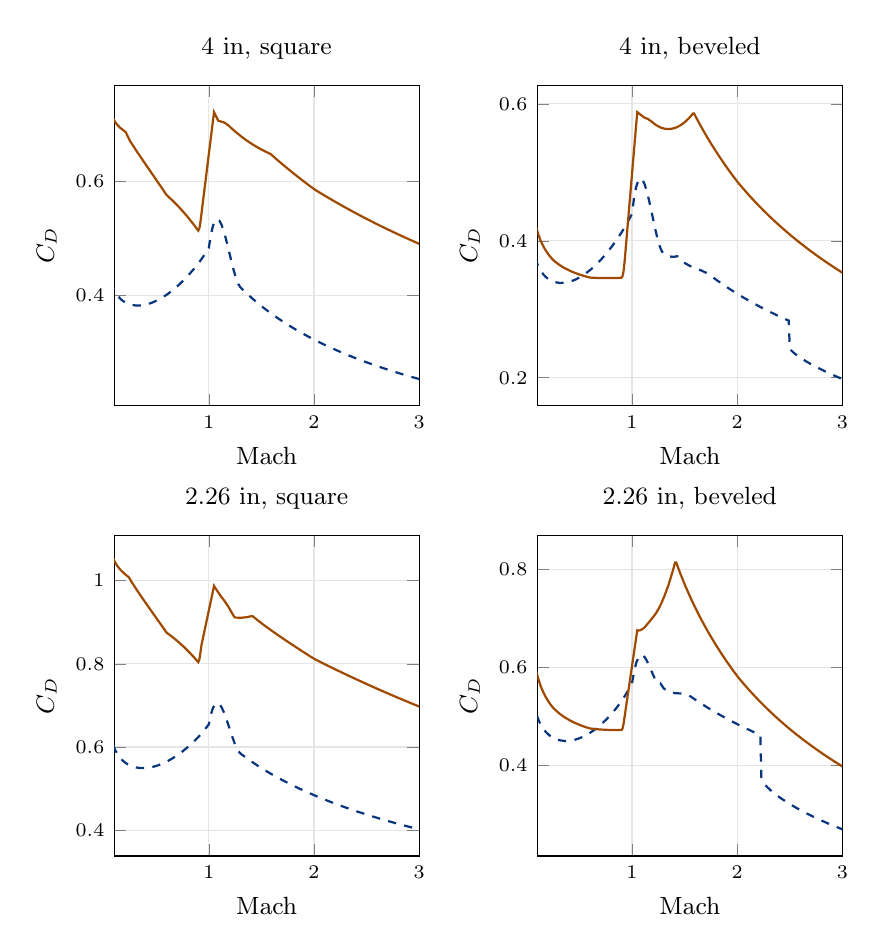
\begin{tikzpicture}
\begin{groupplot}[group style={group size=2 by 2,horizontal sep=1.50cm,vertical sep=1.65cm},width=.45\textwidth,height=5.65cm,grid=major,grid style={gray!20},tick label style={font=\scriptsize},label style={font=\small},title style={font=\small},scaled y ticks=false,yticklabel style={/pgf/number format/fixed,/pgf/number format/precision=3},unbounded coords=jump]
\nextgroupplot[title={4 in, square},xlabel={Mach},ylabel={$C_D$},xmin=0.1,xmax=3]
\addplot[thick,B,dashed] coordinates {(0.01,0.5392703) (0.02,0.4900503) (0.03,0.4658697) (0.04,0.450449) (0.05,0.4393925) (0.06,0.4309168) (0.07,0.424134) (0.08,0.4185425) (0.09,0.4138331) (0.11,0.4063117) (0.13,0.4005716) (0.16,0.3941944) (0.18,0.3910132) (0.21,0.3874247) (0.23,0.3856667) (0.26,0.3838032) (0.31,0.3823806) (0.36,0.3826665) (0.41,0.3843774) (0.46,0.3873356) (0.51,0.3914235) (0.56,0.3965597) (0.61,0.4026861) (0.66,0.40976) (0.71,0.4177495) (0.76,0.4266305) (0.81,0.4363845) (0.86,0.4469972) (0.91,0.4585945) (0.96,0.4716979) (1,0.4829383) (1.01,0.4948939) (1.02,0.5066529) (1.04,0.5223558) (1.06,0.531185) (1.08,0.5340179) (1.1,0.5317335) (1.11,0.5282184) (1.12,0.5247436) (1.14,0.5143528) (1.16,0.5014411) (1.18,0.4868895) (1.21,0.4639718) (1.22,0.4563939) (1.24,0.442215) (1.26,0.4299264) (1.28,0.420412) (1.3,0.4145561) (1.31,0.4127028) (1.36,0.4037825) (1.41,0.3953943) (1.46,0.3874794) (1.51,0.3799903) (1.56,0.3728856) (1.61,0.3661305) (1.66,0.3596946) (1.71,0.3535516) (1.76,0.3476781) (1.81,0.342054) (1.86,0.3366609) (1.91,0.3314828) (1.96,0.3265051) (2.01,0.321715) (2.06,0.3171006) (2.11,0.3126512) (2.16,0.3083573) (2.21,0.3042101) (2.26,0.3002013) (2.31,0.2963238) (2.36,0.2925705) (2.41,0.2889353) (2.46,0.2854124) (2.51,0.2819964) (2.56,0.2786823) (2.61,0.2754654) (2.66,0.2723414) (2.71,0.2693063) (2.76,0.2663562) (2.81,0.2634875) (2.86,0.2606971) (2.91,0.2579816) (2.96,0.2553382) (3,0.2532734)};
\addplot[thick,burntorange] coordinates {(0.01,0.8080247) (0.02,0.7703703) (0.03,0.7516897) (0.04,0.7397161) (0.05,0.7310909) (0.06,0.7244427) (0.07,0.7190856) (0.08,0.7146313) (0.09,0.71084) (0.11,0.7046646) (0.13,0.6997837) (0.16,0.6940281) (0.21,0.6869798) (0.25,0.6717458) (0.26,0.6688288) (0.31,0.6546548) (0.36,0.6409243) (0.41,0.6274162) (0.46,0.6139917) (0.51,0.6005588) (0.56,0.5870533) (0.6,0.5761646) (0.61,0.5745601) (0.66,0.5659074) (0.71,0.5565273) (0.76,0.5463991) (0.81,0.5355068) (0.86,0.5238373) (0.9,0.5139346) (0.91,0.5174294) (0.92,0.5279136) (0.96,0.5879089) (1.01,0.6623833) (1.05,0.7219628) (1.06,0.7181847) (1.09,0.7070495) (1.11,0.7057831) (1.15,0.7035359) (1.16,0.7021903) (1.19,0.6981246) (1.21,0.6946208) (1.26,0.6864266) (1.31,0.6789658) (1.36,0.6721722) (1.41,0.6659967) (1.46,0.660401) (1.51,0.6553543) (1.56,0.6508322) (1.59,0.6480014) (1.61,0.644709) (1.66,0.6366592) (1.71,0.6288397) (1.76,0.6212208) (1.81,0.6137783) (1.86,0.6064927) (1.91,0.5993475) (1.96,0.5923293) (2.01,0.5856607) (2.06,0.5800016) (2.11,0.5744531) (2.16,0.5690102) (2.21,0.5636688) (2.26,0.5584257) (2.31,0.5532778) (2.36,0.5482225) (2.41,0.5432574) (2.46,0.5383803) (2.51,0.533589) (2.56,0.5288813) (2.61,0.5242552) (2.66,0.5197083) (2.71,0.5152385) (2.76,0.5108433) (2.81,0.5065202) (2.86,0.5022668) (2.91,0.4980803) (2.96,0.4939578) (3,0.4907041)};
\nextgroupplot[title={4 in, beveled},xlabel={Mach},ylabel={$C_D$},xmin=0.1,xmax=3]
\addplot[thick,B,dashed] coordinates {(0.01,0.4955621) (0.02,0.4463415) (0.03,0.4221597) (0.04,0.4067373) (0.05,0.3956786) (0.06,0.3872002) (0.07,0.3804143) (0.08,0.3748193) (0.09,0.3701059) (0.11,0.3625749) (0.13,0.3568235) (0.16,0.3504259) (0.18,0.3472289) (0.21,0.3436136) (0.23,0.3418356) (0.26,0.3399392) (0.31,0.3384548) (0.36,0.3386713) (0.41,0.3403069) (0.46,0.3431862) (0.51,0.3471947) (0.56,0.3522544) (0.61,0.3583117) (0.66,0.3653296) (0.71,0.3732834) (0.76,0.3821579) (0.81,0.3919458) (0.86,0.4026476) (0.91,0.4144078) (0.96,0.4277726) (1,0.4393144) (1.01,0.4510799) (1.02,0.4629209) (1.04,0.4788217) (1.06,0.4878998) (1.08,0.4910396) (1.1,0.4891272) (1.11,0.4858248) (1.12,0.4825817) (1.14,0.4727157) (1.16,0.4604176) (1.18,0.4465782) (1.21,0.4249381) (1.22,0.4178484) (1.24,0.404751) (1.26,0.3936996) (1.28,0.3856) (1.3,0.3813638) (1.31,0.3804075) (1.34,0.37809) (1.36,0.3770685) (1.39,0.3764987) (1.41,0.376916) (1.43,0.3775066) (1.46,0.3727592) (1.51,0.366726) (1.56,0.3625256) (1.61,0.3594235) (1.66,0.3565539) (1.71,0.3529445) (1.76,0.3476781) (1.81,0.342054) (1.86,0.3366609) (1.91,0.3314828) (1.96,0.3265051) (2.01,0.321715) (2.06,0.3171006) (2.11,0.3126512) (2.16,0.3083573) (2.21,0.3042101) (2.26,0.3002013) (2.31,0.2963238) (2.36,0.2925705) (2.41,0.2889353) (2.46,0.2854124) (2.49,0.2833503) (2.5,0.2430483) (2.51,0.240604) (2.53,0.2374095) (2.56,0.233615) (2.61,0.2282684) (2.66,0.2235344) (2.71,0.2191793) (2.76,0.2151014) (2.81,0.2112445) (2.86,0.2075729) (2.91,0.2040619) (2.96,0.2006932) (3,0.1980912)};
\addplot[thick,burntorange] coordinates {(0.01,0.5863164) (0.02,0.5211986) (0.03,0.4891801) (0.04,0.4687447) (0.05,0.4540613) (0.06,0.442762) (0.07,0.4336675) (0.08,0.4261116) (0.09,0.4196841) (0.1,0.4141154) (0.11,0.4092202) (0.13,0.4009531) (0.14,0.3974088) (0.16,0.3912058) (0.18,0.3859236) (0.21,0.3792669) (0.24,0.3737261) (0.26,0.3706882) (0.31,0.3647434) (0.36,0.3600281) (0.41,0.3561808) (0.46,0.3529754) (0.51,0.3502616) (0.56,0.3479347) (0.6,0.3463006) (0.61,0.3462077) (0.66,0.3458135) (0.71,0.3455966) (0.76,0.3455285) (0.81,0.3455865) (0.86,0.3457523) (0.9,0.3459527) (0.91,0.3483052) (0.92,0.3553626) (0.93,0.3697444) (0.96,0.4242766) (1.01,0.5151636) (1.05,0.5878732) (1.06,0.5866429) (1.11,0.5807182) (1.13,0.5790303) (1.15,0.5780496) (1.16,0.576851) (1.19,0.5736579) (1.21,0.5710699) (1.23,0.5688669) (1.26,0.5662524) (1.28,0.564955) (1.31,0.5636602) (1.33,0.5632242) (1.36,0.5632031) (1.38,0.5636076) (1.41,0.5648392) (1.43,0.5660756) (1.46,0.5685528) (1.49,0.5717779) (1.51,0.5743443) (1.54,0.5788208) (1.56,0.5822248) (1.58,0.5859661) (1.59,0.5858598) (1.61,0.5799547) (1.66,0.5658094) (1.71,0.5524506) (1.76,0.5397811) (1.81,0.5277226) (1.86,0.5162118) (1.91,0.5051956) (1.96,0.4946296) (2.01,0.4846276) (2.06,0.475588) (2.11,0.4669043) (2.16,0.4585525) (2.21,0.4505112) (2.26,0.4427617) (2.31,0.4352867) (2.36,0.4280706) (2.41,0.4210989) (2.46,0.4143585) (2.51,0.4078372) (2.56,0.4015231) (2.61,0.3954055) (2.66,0.3894743) (2.71,0.3837197) (2.76,0.3781323) (2.81,0.3727032) (2.86,0.3674241) (2.91,0.3622866) (2.96,0.3572828) (3,0.3533708)};
\nextgroupplot[title={2.26 in, square},xlabel={Mach},ylabel={$C_D$},xmin=0.1,xmax=3]
\addplot[thick,B,dashed] coordinates {(0.01,0.8020017) (0.02,0.7245741) (0.03,0.686642) (0.04,0.6624746) (0.05,0.6451456) (0.06,0.6318502) (0.07,0.6211938) (0.08,0.6123893) (0.09,0.604952) (0.1,0.5985638) (0.11,0.5930054) (0.13,0.5837918) (0.16,0.5733641) (0.18,0.5680205) (0.21,0.5617585) (0.23,0.5585117) (0.26,0.5547559) (0.31,0.5508767) (0.36,0.549358) (0.41,0.5497589) (0.46,0.5518042) (0.51,0.5553118) (0.56,0.5601566) (0.61,0.5662493) (0.66,0.5735252) (0.71,0.5819362) (0.76,0.5914465) (0.81,0.602029) (0.86,0.6136636) (0.91,0.6265437) (0.96,0.6414652) (1,0.654376) (1.01,0.6666112) (1.02,0.6783271) (1.04,0.6939761) (1.06,0.7027898) (1.08,0.7056421) (1.1,0.7034092) (1.11,0.6998117) (1.12,0.696256) (1.14,0.6857068) (1.16,0.6726397) (1.18,0.6579336) (1.21,0.634783) (1.24,0.6127886) (1.26,0.6003375) (1.28,0.5906565) (1.3,0.5846293) (1.31,0.5826885) (1.36,0.573312) (1.41,0.5644364) (1.46,0.5560049) (1.51,0.547972) (1.56,0.5402991) (1.61,0.5329543) (1.66,0.5259098) (1.71,0.5191422) (1.76,0.5126306) (1.81,0.5063573) (1.86,0.5003061) (1.91,0.494463) (1.96,0.4888153) (2.01,0.4833517) (2.06,0.478062) (2.11,0.4729368) (2.16,0.4679677) (2.21,0.463147) (2.26,0.4584675) (2.31,0.4539226) (2.36,0.4495064) (2.41,0.4452132) (2.46,0.4410376) (2.51,0.436975) (2.56,0.4330207) (2.61,0.4291704) (2.66,0.4254201) (2.71,0.4217661) (2.76,0.4182047) (2.81,0.4147327) (2.86,0.4113467) (2.91,0.4080438) (2.96,0.4048212) (3,0.4022989)};
\addplot[thick,burntorange] coordinates {(0.01,1.21345) (0.02,1.15217) (0.03,1.121582) (0.04,1.101885) (0.05,1.087644) (0.06,1.076632) (0.07,1.067733) (0.08,1.060314) (0.09,1.053986) (0.11,1.043646) (0.13,1.035442) (0.16,1.02573) (0.21,1.01377) (0.24,1.008194) (0.26,0.9992) (0.31,0.9796375) (0.36,0.9609273) (0.41,0.9427009) (0.46,0.9247262) (0.51,0.9068487) (0.56,0.8889601) (0.6,0.8745881) (0.61,0.8728513) (0.66,0.8632907) (0.71,0.8528037) (0.76,0.8413554) (0.81,0.828918) (0.86,0.8154694) (0.9,0.8039702) (0.91,0.8094372) (0.92,0.8258382) (0.93,0.8440995) (0.96,0.8798626) (1.01,0.9394678) (1.05,0.987152) (1.06,0.9829413) (1.11,0.9638933) (1.15,0.9508898) (1.16,0.9469838) (1.19,0.9354468) (1.21,0.9264695) (1.24,0.9136873) (1.25,0.911202) (1.26,0.9109504) (1.31,0.9106605) (1.36,0.9119237) (1.41,0.9146808) (1.42,0.9137596) (1.46,0.905556) (1.51,0.8957788) (1.56,0.8864102) (1.61,0.8773532) (1.66,0.8685357) (1.71,0.8599042) (1.76,0.8514182) (1.81,0.8430476) (1.86,0.8347701) (1.91,0.8265688) (1.96,0.8184316) (2.01,0.8106998) (2.06,0.8043691) (2.11,0.7981008) (2.16,0.7918947) (2.21,0.785751) (2.26,0.7796708) (2.31,0.7736552) (2.36,0.7677052) (2.41,0.7618215) (2.46,0.7560053) (2.51,0.7502567) (2.56,0.7445758) (2.61,0.7389624) (2.66,0.7334156) (2.71,0.7279346) (2.76,0.7225177) (2.81,0.7171629) (2.86,0.7118681) (2.91,0.7066306) (2.96,0.7014473) (3,0.6973375)};
\nextgroupplot[title={2.26 in, beveled},xlabel={Mach},ylabel={$C_D$},xmin=0.1,xmax=3]
\addplot[thick,B,dashed] coordinates {(0.01,0.7026778) (0.02,0.6252501) (0.03,0.5873178) (0.04,0.5631501) (0.05,0.5458206) (0.06,0.5325248) (0.07,0.5218679) (0.08,0.5130628) (0.09,0.5056248) (0.11,0.4936768) (0.13,0.4844618) (0.16,0.4740324) (0.18,0.4686881) (0.21,0.4624263) (0.23,0.4591809) (0.26,0.4554296) (0.31,0.451568) (0.36,0.4500849) (0.41,0.4505481) (0.46,0.4526929) (0.51,0.4563512) (0.56,0.4614147) (0.61,0.467816) (0.66,0.4755179) (0.71,0.4845079) (0.76,0.4947961) (0.81,0.5064156) (0.86,0.5194266) (0.91,0.5341312) (0.96,0.5514768) (1,0.5669007) (1.01,0.579224) (1.02,0.5916759) (1.04,0.6089701) (1.06,0.6196922) (1.08,0.624758) (1.1,0.6250922) (1.11,0.6229284) (1.12,0.6209173) (1.14,0.6138277) (1.16,0.6047883) (1.21,0.5802996) (1.22,0.576058) (1.24,0.5695491) (1.26,0.5665903) (1.27,0.567274) (1.3,0.5576188) (1.31,0.5558206) (1.33,0.5528389) (1.36,0.5497526) (1.41,0.5474347) (1.46,0.546845) (1.51,0.5454447) (1.54,0.5429981) (1.56,0.5402991) (1.61,0.5329543) (1.66,0.5259098) (1.71,0.5191422) (1.76,0.5126306) (1.81,0.5063573) (1.86,0.5003061) (1.91,0.494463) (1.96,0.4888153) (2.01,0.4833517) (2.06,0.478062) (2.11,0.4729368) (2.16,0.4679677) (2.21,0.463147) (2.22,0.4622) (2.23,0.3736896) (2.24,0.3685991) (2.26,0.3622825) (2.28,0.3573525) (2.31,0.3510586) (2.36,0.3420837) (2.41,0.3341971) (2.46,0.3270167) (2.51,0.3203572) (2.56,0.3141106) (2.61,0.3082067) (2.66,0.3025961) (2.71,0.2972425) (2.76,0.2921178) (2.81,0.2871996) (2.86,0.2824696) (2.91,0.2779126) (2.96,0.2735157) (3,0.2701059)};
\addplot[thick,burntorange] coordinates {(0.01,0.8502291) (0.02,0.7500316) (0.03,0.7005872) (0.04,0.6689448) (0.05,0.6461587) (0.06,0.6285909) (0.07,0.6144273) (0.08,0.6026425) (0.09,0.5926037) (0.1,0.5838954) (0.11,0.5762313) (0.13,0.5632676) (0.14,0.5577012) (0.16,0.5479464) (0.18,0.5396255) (0.21,0.5291198) (0.24,0.5203569) (0.26,0.5155081) (0.31,0.5058939) (0.36,0.4982169) (0.41,0.4919111) (0.46,0.4866213) (0.51,0.4821112) (0.56,0.4782162) (0.61,0.4752168) (0.66,0.4741182) (0.71,0.47331) (0.76,0.4727461) (0.81,0.4723897) (0.86,0.4722117) (0.9,0.4721813) (0.91,0.4753922) (0.92,0.4850247) (0.96,0.5435473) (1.01,0.6168306) (1.05,0.6754572) (1.06,0.6749282) (1.08,0.6755975) (1.11,0.6795852) (1.13,0.6838852) (1.16,0.6916455) (1.21,0.7048008) (1.23,0.7109227) (1.26,0.7221127) (1.28,0.7308994) (1.31,0.7460596) (1.34,0.7635931) (1.36,0.7766027) (1.39,0.798106) (1.41,0.8137736) (1.42,0.8137167) (1.46,0.7906987) (1.51,0.7643288) (1.56,0.7401393) (1.61,0.7177466) (1.66,0.6968658) (1.71,0.6772797) (1.76,0.6588187) (1.81,0.6413474) (1.86,0.6247559) (1.91,0.6089533) (1.96,0.5938635) (2.01,0.5796419) (2.06,0.5668599) (2.11,0.554629) (2.16,0.5429089) (2.21,0.5316634) (2.26,0.5208607) (2.31,0.5104719) (2.36,0.500471) (2.41,0.4908337) (2.46,0.4815383) (2.51,0.4725643) (2.56,0.4638924) (2.61,0.455505) (2.66,0.447385) (2.71,0.4395167) (2.76,0.4318847) (2.81,0.4244746) (2.86,0.4172726) (2.91,0.4102652) (2.96,0.4034396) (3,0.3981016)};
\end{groupplot}\end{tikzpicture}
\caption{All surfaces have zero roughness; all-turbulent flow is selected. Direct installed-engine curves, without correction.}\label{fig:atlas-01-baseline-cd}
\end{figure}
\noindent{\footnotesize Export files: \code{01-baseline-cd.svg} and \code{01-baseline-cd.png}.\\ Directory: \code{aerodynamic-investigation/extended/figures/}.}

\clearpage\subsubsection*{Transonic drag detail}
\begin{figure}[H]\centering
{\footnotesize\begin{tabular}{ll}
\tikz[baseline=-.5ex]{\draw[thick,B,dashed] (0,0)--(.40,0);}\ MIT OR & \tikz[baseline=-.5ex]{\draw[thick,burntorange] (0,0)--(.40,0);}\ RASAero\\
\end{tabular}}\par\vspace{.7em}
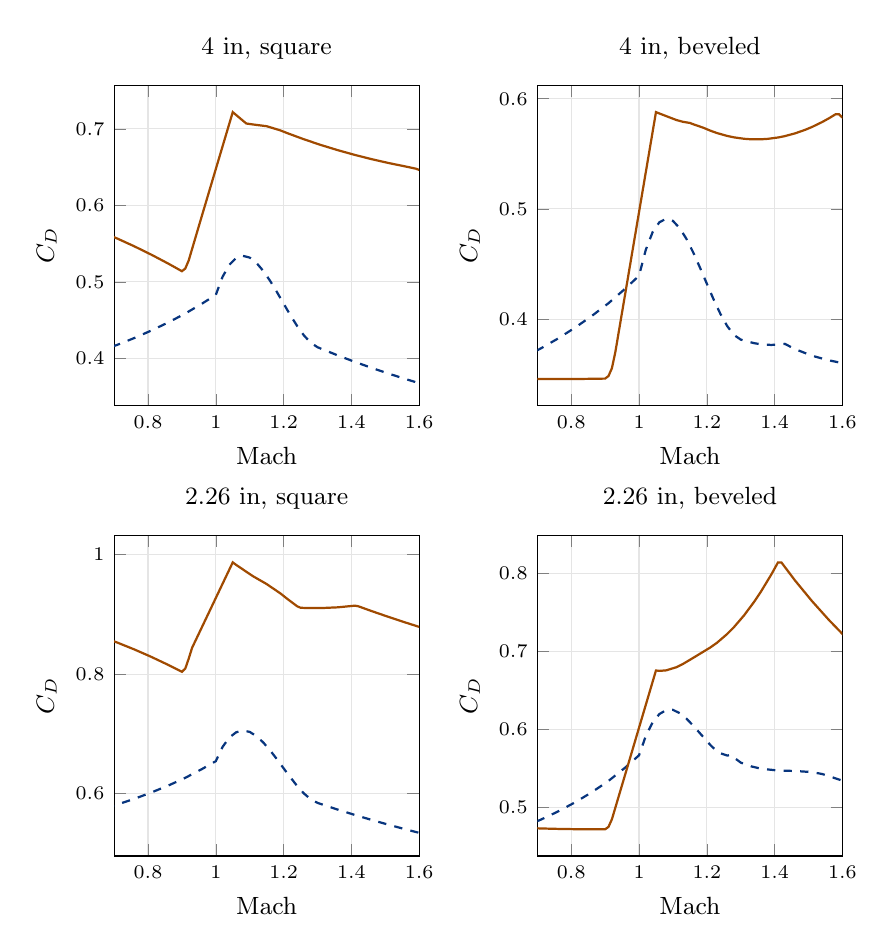
\begin{tikzpicture}
\begin{groupplot}[group style={group size=2 by 2,horizontal sep=1.50cm,vertical sep=1.65cm},width=.45\textwidth,height=5.65cm,grid=major,grid style={gray!20},tick label style={font=\scriptsize},label style={font=\small},title style={font=\small},scaled y ticks=false,yticklabel style={/pgf/number format/fixed,/pgf/number format/precision=3},unbounded coords=jump]
\nextgroupplot[title={4 in, square},xlabel={Mach},ylabel={$C_D$},xmin=0.7,xmax=1.6]
\addplot[thick,B,dashed] coordinates {(0.01,0.5392703) (0.02,0.4900503) (0.03,0.4658697) (0.04,0.450449) (0.05,0.4393925) (0.06,0.4309168) (0.07,0.424134) (0.08,0.4185425) (0.09,0.4138331) (0.11,0.4063117) (0.13,0.4005716) (0.16,0.3941944) (0.18,0.3910132) (0.21,0.3874247) (0.23,0.3856667) (0.26,0.3838032) (0.31,0.3823806) (0.36,0.3826665) (0.41,0.3843774) (0.46,0.3873356) (0.51,0.3914235) (0.56,0.3965597) (0.61,0.4026861) (0.66,0.40976) (0.71,0.4177495) (0.76,0.4266305) (0.81,0.4363845) (0.86,0.4469972) (0.91,0.4585945) (0.96,0.4716979) (1,0.4829383) (1.01,0.4948939) (1.02,0.5066529) (1.04,0.5223558) (1.06,0.531185) (1.08,0.5340179) (1.1,0.5317335) (1.11,0.5282184) (1.12,0.5247436) (1.14,0.5143528) (1.16,0.5014411) (1.18,0.4868895) (1.21,0.4639718) (1.22,0.4563939) (1.24,0.442215) (1.26,0.4299264) (1.28,0.420412) (1.3,0.4145561) (1.31,0.4127028) (1.36,0.4037825) (1.41,0.3953943) (1.46,0.3874794) (1.51,0.3799903) (1.56,0.3728856) (1.61,0.3661305) (1.66,0.3596946) (1.71,0.3535516) (1.76,0.3476781) (1.81,0.342054) (1.86,0.3366609) (1.91,0.3314828) (1.96,0.3265051) (2.01,0.321715) (2.06,0.3171006) (2.11,0.3126512) (2.16,0.3083573) (2.21,0.3042101) (2.26,0.3002013) (2.31,0.2963238) (2.36,0.2925705) (2.41,0.2889353) (2.46,0.2854124) (2.51,0.2819964) (2.56,0.2786823) (2.61,0.2754654) (2.66,0.2723414) (2.71,0.2693063) (2.76,0.2663562) (2.81,0.2634875) (2.86,0.2606971) (2.91,0.2579816) (2.96,0.2553382) (3,0.2532734)};
\addplot[thick,burntorange] coordinates {(0.01,0.8080247) (0.02,0.7703703) (0.03,0.7516897) (0.04,0.7397161) (0.05,0.7310909) (0.06,0.7244427) (0.07,0.7190856) (0.08,0.7146313) (0.09,0.71084) (0.11,0.7046646) (0.13,0.6997837) (0.16,0.6940281) (0.21,0.6869798) (0.25,0.6717458) (0.26,0.6688288) (0.31,0.6546548) (0.36,0.6409243) (0.41,0.6274162) (0.46,0.6139917) (0.51,0.6005588) (0.56,0.5870533) (0.6,0.5761646) (0.61,0.5745601) (0.66,0.5659074) (0.71,0.5565273) (0.76,0.5463991) (0.81,0.5355068) (0.86,0.5238373) (0.9,0.5139346) (0.91,0.5174294) (0.92,0.5279136) (0.96,0.5879089) (1.01,0.6623833) (1.05,0.7219628) (1.06,0.7181847) (1.09,0.7070495) (1.11,0.7057831) (1.15,0.7035359) (1.16,0.7021903) (1.19,0.6981246) (1.21,0.6946208) (1.26,0.6864266) (1.31,0.6789658) (1.36,0.6721722) (1.41,0.6659967) (1.46,0.660401) (1.51,0.6553543) (1.56,0.6508322) (1.59,0.6480014) (1.61,0.644709) (1.66,0.6366592) (1.71,0.6288397) (1.76,0.6212208) (1.81,0.6137783) (1.86,0.6064927) (1.91,0.5993475) (1.96,0.5923293) (2.01,0.5856607) (2.06,0.5800016) (2.11,0.5744531) (2.16,0.5690102) (2.21,0.5636688) (2.26,0.5584257) (2.31,0.5532778) (2.36,0.5482225) (2.41,0.5432574) (2.46,0.5383803) (2.51,0.533589) (2.56,0.5288813) (2.61,0.5242552) (2.66,0.5197083) (2.71,0.5152385) (2.76,0.5108433) (2.81,0.5065202) (2.86,0.5022668) (2.91,0.4980803) (2.96,0.4939578) (3,0.4907041)};
\nextgroupplot[title={4 in, beveled},xlabel={Mach},ylabel={$C_D$},xmin=0.7,xmax=1.6]
\addplot[thick,B,dashed] coordinates {(0.01,0.4955621) (0.02,0.4463415) (0.03,0.4221597) (0.04,0.4067373) (0.05,0.3956786) (0.06,0.3872002) (0.07,0.3804143) (0.08,0.3748193) (0.09,0.3701059) (0.11,0.3625749) (0.13,0.3568235) (0.16,0.3504259) (0.18,0.3472289) (0.21,0.3436136) (0.23,0.3418356) (0.26,0.3399392) (0.31,0.3384548) (0.36,0.3386713) (0.41,0.3403069) (0.46,0.3431862) (0.51,0.3471947) (0.56,0.3522544) (0.61,0.3583117) (0.66,0.3653296) (0.71,0.3732834) (0.76,0.3821579) (0.81,0.3919458) (0.86,0.4026476) (0.91,0.4144078) (0.96,0.4277726) (1,0.4393144) (1.01,0.4510799) (1.02,0.4629209) (1.04,0.4788217) (1.06,0.4878998) (1.08,0.4910396) (1.1,0.4891272) (1.11,0.4858248) (1.12,0.4825817) (1.14,0.4727157) (1.16,0.4604176) (1.18,0.4465782) (1.21,0.4249381) (1.22,0.4178484) (1.24,0.404751) (1.26,0.3936996) (1.28,0.3856) (1.3,0.3813638) (1.31,0.3804075) (1.34,0.37809) (1.36,0.3770685) (1.39,0.3764987) (1.41,0.376916) (1.43,0.3775066) (1.46,0.3727592) (1.51,0.366726) (1.56,0.3625256) (1.61,0.3594235) (1.66,0.3565539) (1.71,0.3529445) (1.76,0.3476781) (1.81,0.342054) (1.86,0.3366609) (1.91,0.3314828) (1.96,0.3265051) (2.01,0.321715) (2.06,0.3171006) (2.11,0.3126512) (2.16,0.3083573) (2.21,0.3042101) (2.26,0.3002013) (2.31,0.2963238) (2.36,0.2925705) (2.41,0.2889353) (2.46,0.2854124) (2.49,0.2833503) (2.5,0.2430483) (2.51,0.240604) (2.53,0.2374095) (2.56,0.233615) (2.61,0.2282684) (2.66,0.2235344) (2.71,0.2191793) (2.76,0.2151014) (2.81,0.2112445) (2.86,0.2075729) (2.91,0.2040619) (2.96,0.2006932) (3,0.1980912)};
\addplot[thick,burntorange] coordinates {(0.01,0.5863164) (0.02,0.5211986) (0.03,0.4891801) (0.04,0.4687447) (0.05,0.4540613) (0.06,0.442762) (0.07,0.4336675) (0.08,0.4261116) (0.09,0.4196841) (0.1,0.4141154) (0.11,0.4092202) (0.13,0.4009531) (0.14,0.3974088) (0.16,0.3912058) (0.18,0.3859236) (0.21,0.3792669) (0.24,0.3737261) (0.26,0.3706882) (0.31,0.3647434) (0.36,0.3600281) (0.41,0.3561808) (0.46,0.3529754) (0.51,0.3502616) (0.56,0.3479347) (0.6,0.3463006) (0.61,0.3462077) (0.66,0.3458135) (0.71,0.3455966) (0.76,0.3455285) (0.81,0.3455865) (0.86,0.3457523) (0.9,0.3459527) (0.91,0.3483052) (0.92,0.3553626) (0.93,0.3697444) (0.96,0.4242766) (1.01,0.5151636) (1.05,0.5878732) (1.06,0.5866429) (1.11,0.5807182) (1.13,0.5790303) (1.15,0.5780496) (1.16,0.576851) (1.19,0.5736579) (1.21,0.5710699) (1.23,0.5688669) (1.26,0.5662524) (1.28,0.564955) (1.31,0.5636602) (1.33,0.5632242) (1.36,0.5632031) (1.38,0.5636076) (1.41,0.5648392) (1.43,0.5660756) (1.46,0.5685528) (1.49,0.5717779) (1.51,0.5743443) (1.54,0.5788208) (1.56,0.5822248) (1.58,0.5859661) (1.59,0.5858598) (1.61,0.5799547) (1.66,0.5658094) (1.71,0.5524506) (1.76,0.5397811) (1.81,0.5277226) (1.86,0.5162118) (1.91,0.5051956) (1.96,0.4946296) (2.01,0.4846276) (2.06,0.475588) (2.11,0.4669043) (2.16,0.4585525) (2.21,0.4505112) (2.26,0.4427617) (2.31,0.4352867) (2.36,0.4280706) (2.41,0.4210989) (2.46,0.4143585) (2.51,0.4078372) (2.56,0.4015231) (2.61,0.3954055) (2.66,0.3894743) (2.71,0.3837197) (2.76,0.3781323) (2.81,0.3727032) (2.86,0.3674241) (2.91,0.3622866) (2.96,0.3572828) (3,0.3533708)};
\nextgroupplot[title={2.26 in, square},xlabel={Mach},ylabel={$C_D$},xmin=0.7,xmax=1.6]
\addplot[thick,B,dashed] coordinates {(0.01,0.8020017) (0.02,0.7245741) (0.03,0.686642) (0.04,0.6624746) (0.05,0.6451456) (0.06,0.6318502) (0.07,0.6211938) (0.08,0.6123893) (0.09,0.604952) (0.1,0.5985638) (0.11,0.5930054) (0.13,0.5837918) (0.16,0.5733641) (0.18,0.5680205) (0.21,0.5617585) (0.23,0.5585117) (0.26,0.5547559) (0.31,0.5508767) (0.36,0.549358) (0.41,0.5497589) (0.46,0.5518042) (0.51,0.5553118) (0.56,0.5601566) (0.61,0.5662493) (0.66,0.5735252) (0.71,0.5819362) (0.76,0.5914465) (0.81,0.602029) (0.86,0.6136636) (0.91,0.6265437) (0.96,0.6414652) (1,0.654376) (1.01,0.6666112) (1.02,0.6783271) (1.04,0.6939761) (1.06,0.7027898) (1.08,0.7056421) (1.1,0.7034092) (1.11,0.6998117) (1.12,0.696256) (1.14,0.6857068) (1.16,0.6726397) (1.18,0.6579336) (1.21,0.634783) (1.24,0.6127886) (1.26,0.6003375) (1.28,0.5906565) (1.3,0.5846293) (1.31,0.5826885) (1.36,0.573312) (1.41,0.5644364) (1.46,0.5560049) (1.51,0.547972) (1.56,0.5402991) (1.61,0.5329543) (1.66,0.5259098) (1.71,0.5191422) (1.76,0.5126306) (1.81,0.5063573) (1.86,0.5003061) (1.91,0.494463) (1.96,0.4888153) (2.01,0.4833517) (2.06,0.478062) (2.11,0.4729368) (2.16,0.4679677) (2.21,0.463147) (2.26,0.4584675) (2.31,0.4539226) (2.36,0.4495064) (2.41,0.4452132) (2.46,0.4410376) (2.51,0.436975) (2.56,0.4330207) (2.61,0.4291704) (2.66,0.4254201) (2.71,0.4217661) (2.76,0.4182047) (2.81,0.4147327) (2.86,0.4113467) (2.91,0.4080438) (2.96,0.4048212) (3,0.4022989)};
\addplot[thick,burntorange] coordinates {(0.01,1.21345) (0.02,1.15217) (0.03,1.121582) (0.04,1.101885) (0.05,1.087644) (0.06,1.076632) (0.07,1.067733) (0.08,1.060314) (0.09,1.053986) (0.11,1.043646) (0.13,1.035442) (0.16,1.02573) (0.21,1.01377) (0.24,1.008194) (0.26,0.9992) (0.31,0.9796375) (0.36,0.9609273) (0.41,0.9427009) (0.46,0.9247262) (0.51,0.9068487) (0.56,0.8889601) (0.6,0.8745881) (0.61,0.8728513) (0.66,0.8632907) (0.71,0.8528037) (0.76,0.8413554) (0.81,0.828918) (0.86,0.8154694) (0.9,0.8039702) (0.91,0.8094372) (0.92,0.8258382) (0.93,0.8440995) (0.96,0.8798626) (1.01,0.9394678) (1.05,0.987152) (1.06,0.9829413) (1.11,0.9638933) (1.15,0.9508898) (1.16,0.9469838) (1.19,0.9354468) (1.21,0.9264695) (1.24,0.9136873) (1.25,0.911202) (1.26,0.9109504) (1.31,0.9106605) (1.36,0.9119237) (1.41,0.9146808) (1.42,0.9137596) (1.46,0.905556) (1.51,0.8957788) (1.56,0.8864102) (1.61,0.8773532) (1.66,0.8685357) (1.71,0.8599042) (1.76,0.8514182) (1.81,0.8430476) (1.86,0.8347701) (1.91,0.8265688) (1.96,0.8184316) (2.01,0.8106998) (2.06,0.8043691) (2.11,0.7981008) (2.16,0.7918947) (2.21,0.785751) (2.26,0.7796708) (2.31,0.7736552) (2.36,0.7677052) (2.41,0.7618215) (2.46,0.7560053) (2.51,0.7502567) (2.56,0.7445758) (2.61,0.7389624) (2.66,0.7334156) (2.71,0.7279346) (2.76,0.7225177) (2.81,0.7171629) (2.86,0.7118681) (2.91,0.7066306) (2.96,0.7014473) (3,0.6973375)};
\nextgroupplot[title={2.26 in, beveled},xlabel={Mach},ylabel={$C_D$},xmin=0.7,xmax=1.6]
\addplot[thick,B,dashed] coordinates {(0.01,0.7026778) (0.02,0.6252501) (0.03,0.5873178) (0.04,0.5631501) (0.05,0.5458206) (0.06,0.5325248) (0.07,0.5218679) (0.08,0.5130628) (0.09,0.5056248) (0.11,0.4936768) (0.13,0.4844618) (0.16,0.4740324) (0.18,0.4686881) (0.21,0.4624263) (0.23,0.4591809) (0.26,0.4554296) (0.31,0.451568) (0.36,0.4500849) (0.41,0.4505481) (0.46,0.4526929) (0.51,0.4563512) (0.56,0.4614147) (0.61,0.467816) (0.66,0.4755179) (0.71,0.4845079) (0.76,0.4947961) (0.81,0.5064156) (0.86,0.5194266) (0.91,0.5341312) (0.96,0.5514768) (1,0.5669007) (1.01,0.579224) (1.02,0.5916759) (1.04,0.6089701) (1.06,0.6196922) (1.08,0.624758) (1.1,0.6250922) (1.11,0.6229284) (1.12,0.6209173) (1.14,0.6138277) (1.16,0.6047883) (1.21,0.5802996) (1.22,0.576058) (1.24,0.5695491) (1.26,0.5665903) (1.27,0.567274) (1.3,0.5576188) (1.31,0.5558206) (1.33,0.5528389) (1.36,0.5497526) (1.41,0.5474347) (1.46,0.546845) (1.51,0.5454447) (1.54,0.5429981) (1.56,0.5402991) (1.61,0.5329543) (1.66,0.5259098) (1.71,0.5191422) (1.76,0.5126306) (1.81,0.5063573) (1.86,0.5003061) (1.91,0.494463) (1.96,0.4888153) (2.01,0.4833517) (2.06,0.478062) (2.11,0.4729368) (2.16,0.4679677) (2.21,0.463147) (2.22,0.4622) (2.23,0.3736896) (2.24,0.3685991) (2.26,0.3622825) (2.28,0.3573525) (2.31,0.3510586) (2.36,0.3420837) (2.41,0.3341971) (2.46,0.3270167) (2.51,0.3203572) (2.56,0.3141106) (2.61,0.3082067) (2.66,0.3025961) (2.71,0.2972425) (2.76,0.2921178) (2.81,0.2871996) (2.86,0.2824696) (2.91,0.2779126) (2.96,0.2735157) (3,0.2701059)};
\addplot[thick,burntorange] coordinates {(0.01,0.8502291) (0.02,0.7500316) (0.03,0.7005872) (0.04,0.6689448) (0.05,0.6461587) (0.06,0.6285909) (0.07,0.6144273) (0.08,0.6026425) (0.09,0.5926037) (0.1,0.5838954) (0.11,0.5762313) (0.13,0.5632676) (0.14,0.5577012) (0.16,0.5479464) (0.18,0.5396255) (0.21,0.5291198) (0.24,0.5203569) (0.26,0.5155081) (0.31,0.5058939) (0.36,0.4982169) (0.41,0.4919111) (0.46,0.4866213) (0.51,0.4821112) (0.56,0.4782162) (0.61,0.4752168) (0.66,0.4741182) (0.71,0.47331) (0.76,0.4727461) (0.81,0.4723897) (0.86,0.4722117) (0.9,0.4721813) (0.91,0.4753922) (0.92,0.4850247) (0.96,0.5435473) (1.01,0.6168306) (1.05,0.6754572) (1.06,0.6749282) (1.08,0.6755975) (1.11,0.6795852) (1.13,0.6838852) (1.16,0.6916455) (1.21,0.7048008) (1.23,0.7109227) (1.26,0.7221127) (1.28,0.7308994) (1.31,0.7460596) (1.34,0.7635931) (1.36,0.7766027) (1.39,0.798106) (1.41,0.8137736) (1.42,0.8137167) (1.46,0.7906987) (1.51,0.7643288) (1.56,0.7401393) (1.61,0.7177466) (1.66,0.6968658) (1.71,0.6772797) (1.76,0.6588187) (1.81,0.6413474) (1.86,0.6247559) (1.91,0.6089533) (1.96,0.5938635) (2.01,0.5796419) (2.06,0.5668599) (2.11,0.554629) (2.16,0.5429089) (2.21,0.5316634) (2.26,0.5208607) (2.31,0.5104719) (2.36,0.500471) (2.41,0.4908337) (2.46,0.4815383) (2.51,0.4725643) (2.56,0.4638924) (2.61,0.455505) (2.66,0.447385) (2.71,0.4395167) (2.76,0.4318847) (2.81,0.4244746) (2.86,0.4172726) (2.91,0.4102652) (2.96,0.4034396) (3,0.3981016)};
\end{groupplot}\end{tikzpicture}
\caption{The denser transonic comparison tests the location, width and magnitude of the drag rise, rather than matching one peak.}\label{fig:atlas-02-transonic-cd}
\end{figure}
\noindent{\footnotesize Export files: \code{02-transonic-cd.svg} and \code{02-transonic-cd.png}.\\ Directory: \code{aerodynamic-investigation/extended/figures/}.}

\clearpage\subsubsection*{Drag residuals by Mach}
\begin{figure}[H]\centering
{\footnotesize\begin{tabular}{l}
\tikz[baseline=-.5ex]{\draw[thick,g] (0,0)--(.40,0);}\ RAS - OR\\
\end{tabular}}\par\vspace{.7em}
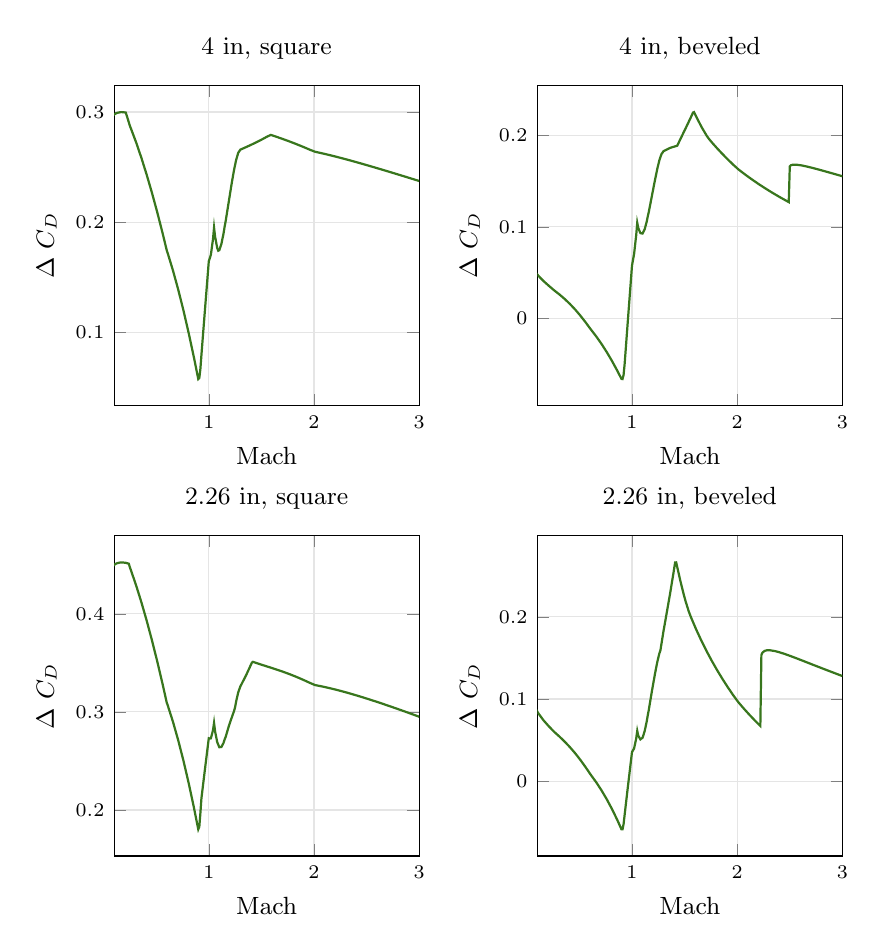
\begin{tikzpicture}
\begin{groupplot}[group style={group size=2 by 2,horizontal sep=1.50cm,vertical sep=1.65cm},width=.45\textwidth,height=5.65cm,grid=major,grid style={gray!20},tick label style={font=\scriptsize},label style={font=\small},title style={font=\small},scaled y ticks=false,yticklabel style={/pgf/number format/fixed,/pgf/number format/precision=3},unbounded coords=jump]
\nextgroupplot[title={4 in, square},xlabel={Mach},ylabel={$\Delta$ $C_D$},xmin=0.1,xmax=3]
\addplot[thick,g] coordinates {(0.01,0.2687545) (0.02,0.2803199) (0.03,0.28582) (0.04,0.289267) (0.05,0.2916984) (0.06,0.2935259) (0.08,0.2960888) (0.11,0.298353) (0.13,0.2992121) (0.16,0.2998337) (0.17,0.2998963) (0.21,0.2995551) (0.22,0.2968555) (0.25,0.2874155) (0.26,0.2850256) (0.31,0.2722742) (0.36,0.2582578) (0.41,0.2430388) (0.46,0.2266561) (0.51,0.2091354) (0.56,0.1904936) (0.6,0.1747808) (0.61,0.171874) (0.66,0.1561474) (0.71,0.1387777) (0.76,0.1197686) (0.81,0.0991223) (0.86,0.07684009) (0.9,0.05783635) (0.91,0.05883484) (0.92,0.0667816) (0.93,0.07951333) (0.96,0.116211) (1,0.1645501) (1.01,0.1674894) (1.02,0.1706253) (1.04,0.1847121) (1.05,0.1952218) (1.06,0.1869997) (1.08,0.1767107) (1.09,0.1742005) (1.1,0.1746706) (1.11,0.1775647) (1.12,0.1804333) (1.14,0.1896774) (1.15,0.1956568) (1.16,0.2007491) (1.21,0.230649) (1.22,0.2365253) (1.24,0.2473967) (1.26,0.2565002) (1.28,0.2629465) (1.3,0.2658467) (1.31,0.266263) (1.36,0.2683897) (1.41,0.2706025) (1.46,0.2729216) (1.51,0.2753639) (1.56,0.2779466) (1.59,0.2792088) (1.61,0.2785785) (1.66,0.2769646) (1.71,0.2752881) (1.76,0.2735426) (1.81,0.2717243) (1.86,0.2698318) (1.91,0.2678647) (1.96,0.2658241) (2.01,0.2639457) (2.06,0.2629011) (2.11,0.2618018) (2.16,0.2606529) (2.21,0.2594588) (2.26,0.2582244) (2.31,0.256954) (2.36,0.255652) (2.41,0.254322) (2.46,0.2529678) (2.51,0.2515926) (2.56,0.250199) (2.61,0.2487898) (2.66,0.2473669) (2.71,0.2459322) (2.76,0.2444871) (2.81,0.2430327) (2.86,0.2415698) (2.91,0.2400987) (2.96,0.2386197) (3,0.2374307)};
\nextgroupplot[title={4 in, beveled},xlabel={Mach},ylabel={$\Delta$ $C_D$},xmin=0.1,xmax=3]
\addplot[thick,g] coordinates {(0.01,0.09075427) (0.02,0.0748571) (0.03,0.06702047) (0.04,0.06200742) (0.05,0.05838276) (0.06,0.05556179) (0.08,0.05129234) (0.11,0.04664532) (0.16,0.04077992) (0.21,0.03565335) (0.26,0.030749) (0.31,0.02628867) (0.36,0.02135681) (0.41,0.01587394) (0.46,0.009789138) (0.51,0.003066913) (0.56,-0.004319629) (0.61,-0.01210399) (0.66,-0.01951616) (0.71,-0.0276868) (0.76,-0.03662935) (0.81,-0.04635935) (0.86,-0.05689528) (0.9,-0.06591931) (0.91,-0.06610267) (0.92,-0.06162623) (0.93,-0.049871) (0.96,-0.003496006) (1,0.05767175) (1.01,0.0640837) (1.02,0.07042006) (1.04,0.09087407) (1.05,0.1045486) (1.06,0.09874308) (1.08,0.09318945) (1.1,0.09274724) (1.11,0.09489335) (1.12,0.0971638) (1.13,0.1014111) (1.14,0.1057584) (1.15,0.1115124) (1.16,0.1164334) (1.21,0.1461318) (1.24,0.1631538) (1.26,0.1725528) (1.28,0.179355) (1.3,0.182642) (1.31,0.1832527) (1.36,0.1861346) (1.41,0.1879232) (1.43,0.1885689) (1.46,0.1957936) (1.51,0.2076182) (1.56,0.2196992) (1.58,0.2247673) (1.59,0.2252745) (1.61,0.2205312) (1.66,0.2092555) (1.71,0.1995061) (1.73,0.1962461) (1.76,0.1921029) (1.81,0.1856686) (1.86,0.1795509) (1.91,0.1737128) (1.96,0.1681245) (2.01,0.1629126) (2.06,0.1584874) (2.11,0.154253) (2.16,0.1501951) (2.21,0.1463011) (2.26,0.1425604) (2.31,0.1389629) (2.36,0.1355001) (2.41,0.1321635) (2.46,0.1289461) (2.49,0.1270698) (2.5,0.1660762) (2.51,0.1672331) (2.53,0.1678777) (2.56,0.167908) (2.61,0.1671371) (2.66,0.1659399) (2.71,0.1645404) (2.76,0.1630309) (2.81,0.1614587) (2.86,0.1598512) (2.91,0.1582247) (2.96,0.1565896) (3,0.1552796)};
\nextgroupplot[title={2.26 in, square},xlabel={Mach},ylabel={$\Delta$ $C_D$},xmin=0.1,xmax=3]
\addplot[thick,g] coordinates {(0.01,0.4114487) (0.02,0.4275963) (0.03,0.4349397) (0.04,0.4394108) (0.05,0.4424985) (0.06,0.4447813) (0.08,0.4479252) (0.11,0.4506403) (0.13,0.4516505) (0.16,0.4523655) (0.17,0.4524328) (0.21,0.4520111) (0.24,0.4510719) (0.25,0.4473901) (0.26,0.4444442) (0.31,0.4287608) (0.36,0.4115693) (0.41,0.3929419) (0.46,0.372922) (0.51,0.3515369) (0.56,0.3288036) (0.6,0.3096538) (0.61,0.306602) (0.66,0.2897655) (0.71,0.2708675) (0.76,0.249909) (0.81,0.226889) (0.86,0.2018058) (0.9,0.1802516) (0.91,0.1828935) (0.92,0.1964167) (0.93,0.2117473) (0.96,0.2383973) (1,0.2731708) (1.01,0.2728566) (1.02,0.2730617) (1.04,0.2812549) (1.05,0.2888028) (1.06,0.2801515) (1.08,0.2691649) (1.1,0.2639953) (1.11,0.2640815) (1.12,0.2642364) (1.13,0.2662327) (1.14,0.2682884) (1.15,0.2717346) (1.16,0.2743442) (1.19,0.2852613) (1.21,0.2916865) (1.24,0.3008988) (1.25,0.3046521) (1.26,0.310613) (1.28,0.3199867) (1.3,0.3259625) (1.31,0.327972) (1.36,0.3386117) (1.41,0.3502444) (1.42,0.3510436) (1.46,0.3495511) (1.51,0.3478069) (1.56,0.3461111) (1.61,0.3443989) (1.66,0.3426259) (1.71,0.340762) (1.76,0.3387875) (1.81,0.3366903) (1.86,0.334464) (1.91,0.3321058) (1.96,0.3296163) (2.01,0.327348) (2.06,0.3263071) (2.11,0.325164) (2.16,0.3239269) (2.21,0.322604) (2.26,0.3212034) (2.31,0.3197325) (2.36,0.3181988) (2.41,0.3166084) (2.46,0.3149676) (2.51,0.3132817) (2.56,0.3115551) (2.61,0.309792) (2.66,0.3079955) (2.71,0.3061685) (2.76,0.3043129) (2.81,0.3024302) (2.86,0.3005214) (2.91,0.2985868) (2.96,0.2966261) (3,0.2950386)};
\nextgroupplot[title={2.26 in, beveled},xlabel={Mach},ylabel={$\Delta$ $C_D$},xmin=0.1,xmax=3]
\addplot[thick,g] coordinates {(0.01,0.1475513) (0.02,0.1247815) (0.03,0.1132694) (0.04,0.1057947) (0.05,0.1003381) (0.06,0.09606611) (0.08,0.08957968) (0.11,0.08255443) (0.16,0.07391407) (0.21,0.06669348) (0.26,0.06007852) (0.31,0.05432595) (0.36,0.04813202) (0.41,0.04136305) (0.46,0.03392843) (0.51,0.02576004) (0.56,0.01680154) (0.61,0.007400838) (0.66,-0.001399725) (0.71,-0.01119789) (0.76,-0.02204997) (0.81,-0.03402588) (0.86,-0.04721491) (0.9,-0.05871748) (0.91,-0.05873899) (0.92,-0.05241532) (0.96,-0.007929473) (1,0.03527322) (1.01,0.03760658) (1.02,0.03981135) (1.04,0.05183041) (1.05,0.06119521) (1.06,0.05523602) (1.08,0.05083951) (1.1,0.05281647) (1.11,0.05665674) (1.12,0.06066466) (1.13,0.06659711) (1.14,0.07265638) (1.15,0.08015762) (1.16,0.08685719) (1.19,0.1100721) (1.21,0.1245012) (1.22,0.1316691) (1.24,0.1448372) (1.26,0.1555224) (1.27,0.1590998) (1.3,0.1831236) (1.31,0.190239) (1.36,0.2268502) (1.39,0.2500774) (1.41,0.2663389) (1.42,0.2664639) (1.46,0.2438537) (1.49,0.2283061) (1.51,0.2188842) (1.54,0.2065825) (1.56,0.1998402) (1.61,0.1847923) (1.66,0.170956) (1.71,0.1581375) (1.76,0.1461881) (1.81,0.1349901) (1.86,0.1244498) (1.91,0.1144903) (1.96,0.1050482) (2.01,0.09629012) (2.06,0.08879787) (2.11,0.0816922) (2.16,0.07494115) (2.21,0.06851637) (2.22,0.06726839) (2.23,0.1536013) (2.24,0.1565314) (2.26,0.1585782) (2.28,0.1593045) (2.31,0.1594133) (2.36,0.1583873) (2.41,0.1566367) (2.46,0.1545216) (2.51,0.1522071) (2.56,0.1497818) (2.61,0.1472983) (2.66,0.1447889) (2.71,0.1422742) (2.76,0.1397669) (2.81,0.137275) (2.86,0.134803) (2.91,0.1323526) (2.96,0.1299238) (3,0.1279956)};
\end{groupplot}\end{tikzpicture}
\caption{Positive residual means RASAero predicts more drag. The sign and size vary with geometry and Mach.}\label{fig:atlas-03-baseline-residual}
\end{figure}
\noindent{\footnotesize Export files: \code{03-baseline-residual.svg} and \code{03-baseline-residual.png}.\\ Directory: \code{aerodynamic-investigation/extended/figures/}.}

\clearpage\subsubsection*{Nose shapes at L/D = 1.5}
\begin{figure}[H]\centering
{\footnotesize\begin{tabular}{ll}
\tikz[baseline=-.5ex]{\draw[thick,B,dashed] (0,0)--(.40,0);}\ MIT OR & \tikz[baseline=-.5ex]{\draw[thick,burntorange] (0,0)--(.40,0);}\ RASAero\\
\end{tabular}}\par\vspace{.7em}
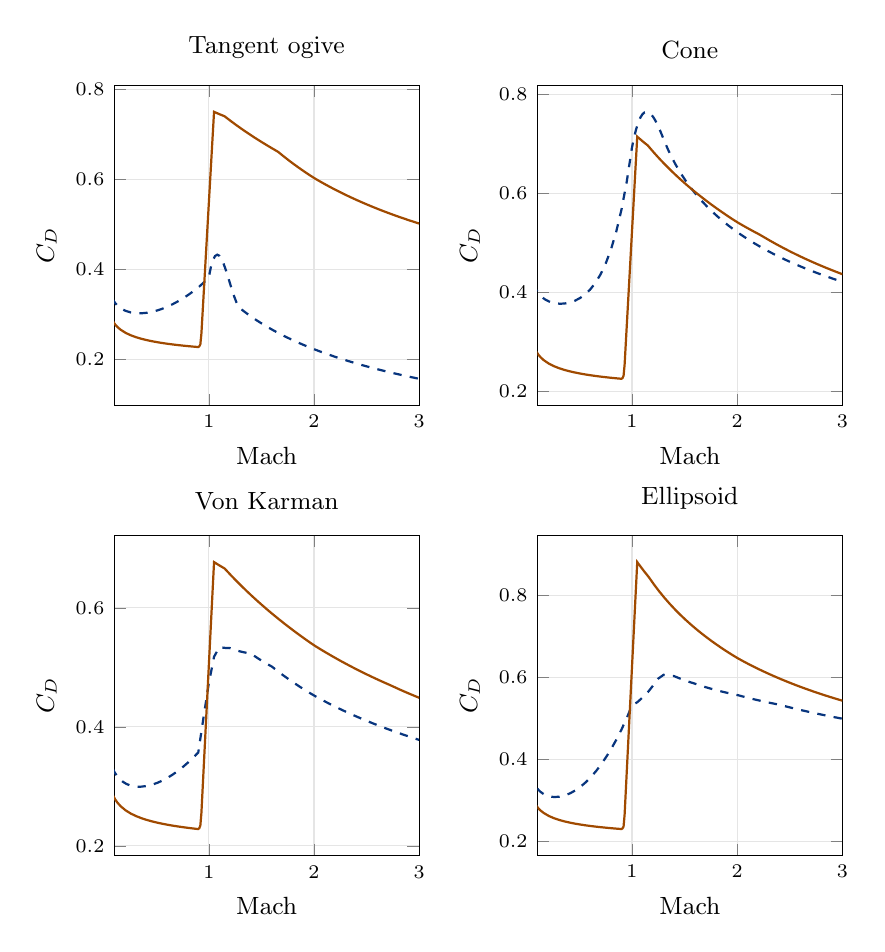
\begin{tikzpicture}
\begin{groupplot}[group style={group size=2 by 2,horizontal sep=1.50cm,vertical sep=1.65cm},width=.45\textwidth,height=5.65cm,grid=major,grid style={gray!20},tick label style={font=\scriptsize},label style={font=\small},title style={font=\small},scaled y ticks=false,yticklabel style={/pgf/number format/fixed,/pgf/number format/precision=3},unbounded coords=jump]
\nextgroupplot[title={Tangent ogive},xlabel={Mach},ylabel={$C_D$},xmin=0.1,xmax=3]
\addplot[thick,B,dashed] coordinates {(0.01,0.4455416) (0.02,0.4012453) (0.03,0.3794793) (0.04,0.365594) (0.05,0.3556335) (0.06,0.3479931) (0.07,0.3418738) (0.08,0.3368241) (0.09,0.3325658) (0.11,0.3257494) (0.13,0.3205265) (0.16,0.3146834) (0.18,0.311739) (0.21,0.3083691) (0.26,0.3048268) (0.31,0.3032015) (0.36,0.3030512) (0.41,0.3041195) (0.46,0.3062456) (0.51,0.3093224) (0.56,0.3132751) (0.61,0.3180498) (0.66,0.3236065) (0.71,0.3299145) (0.76,0.3369502) (0.81,0.3446946) (0.86,0.3531328) (0.91,0.3623754) (0.96,0.3728891) (1,0.3819195) (1.01,0.3936675) (1.02,0.4054734) (1.04,0.4212459) (1.06,0.4301177) (1.08,0.4329704) (1.1,0.4306864) (1.11,0.4271879) (1.12,0.4237274) (1.14,0.4133581) (1.16,0.4004608) (1.18,0.3859184) (1.21,0.3630087) (1.22,0.3554325) (1.24,0.3412569) (1.26,0.3289722) (1.28,0.3194633) (1.3,0.3136153) (1.31,0.3117676) (1.36,0.3028855) (1.41,0.2945556) (1.46,0.2867165) (1.51,0.2793199) (1.56,0.2723222) (1.61,0.2656876) (1.66,0.2593837) (1.71,0.2533831) (1.76,0.247661) (1.81,0.2421959) (1.86,0.2369684) (1.91,0.2319614) (1.96,0.2271595) (2.01,0.2225488) (2.06,0.2181168) (2.11,0.2138522) (2.16,0.2097447) (2.21,0.2057851) (2.26,0.2019646) (2.31,0.1982757) (2.36,0.1947109) (2.41,0.1912638) (2.46,0.1879283) (2.51,0.1846987) (2.56,0.1815698) (2.61,0.1785367) (2.66,0.1755951) (2.71,0.1727406) (2.76,0.1699694) (2.81,0.1672777) (2.86,0.1646623) (2.91,0.1621197) (2.96,0.1596471) (3,0.1577174)};
\addplot[thick,burntorange] coordinates {(0.01,0.3860854) (0.02,0.3468013) (0.03,0.3272929) (0.04,0.3147798) (0.05,0.305761) (0.06,0.298806) (0.08,0.2885359) (0.11,0.2780948) (0.13,0.2729779) (0.16,0.2669406) (0.21,0.2595415) (0.26,0.2541081) (0.31,0.2498676) (0.36,0.2464209) (0.41,0.2435365) (0.46,0.2410692) (0.51,0.2389224) (0.56,0.2370286) (0.61,0.2353391) (0.66,0.2338178) (0.71,0.2324368) (0.76,0.2311748) (0.81,0.2300145) (0.86,0.2289423) (0.9,0.2281403) (0.91,0.2296917) (0.92,0.2343458) (0.93,0.2583182) (0.96,0.3812099) (1.01,0.5860293) (1.05,0.7498849) (1.06,0.7488401) (1.11,0.7438373) (1.15,0.7400742) (1.16,0.738272) (1.21,0.7293176) (1.26,0.720705) (1.31,0.7124021) (1.36,0.7043815) (1.41,0.6966204) (1.46,0.689099) (1.51,0.6818004) (1.56,0.67471) (1.61,0.6678149) (1.66,0.6609771) (1.71,0.651455) (1.76,0.6423363) (1.81,0.6335876) (1.86,0.6251795) (1.91,0.6170865) (1.96,0.6092854) (2.01,0.601863) (2.06,0.5951049) (2.11,0.5885878) (2.16,0.582298) (2.21,0.5762228) (2.26,0.5703513) (2.31,0.564673) (2.36,0.5591789) (2.41,0.5538602) (2.46,0.5487092) (2.51,0.5437186) (2.56,0.5388815) (2.61,0.5341919) (2.66,0.529644) (2.71,0.5252321) (2.76,0.5209512) (2.81,0.5167965) (2.86,0.5127635) (2.91,0.5088478) (2.96,0.5050453) (3,0.5020823)};
\nextgroupplot[title={Cone},xlabel={Mach},ylabel={$C_D$},xmin=0.1,xmax=3]
\addplot[thick,B,dashed] coordinates {(0.01,0.5164651) (0.02,0.4730041) (0.03,0.4516495) (0.04,0.4380274) (0.05,0.4282568) (0.06,0.4207632) (0.07,0.4147625) (0.08,0.4098118) (0.09,0.4056381) (0.11,0.3989613) (0.13,0.393851) (0.16,0.3881472) (0.18,0.3852858) (0.21,0.3820352) (0.26,0.3787228) (0.31,0.3774422) (0.32,0.3774066) (0.36,0.3778736) (0.41,0.3799348) (0.46,0.3837065) (0.51,0.3894063) (0.56,0.3973833) (0.6,0.4055187) (0.61,0.4081237) (0.65,0.4188525) (0.66,0.4222609) (0.7,0.4361918) (0.71,0.4405899) (0.75,0.4584707) (0.76,0.4640833) (0.8,0.4868154) (0.81,0.4939096) (0.85,0.5225628) (0.86,0.5314521) (0.9,0.5672808) (0.91,0.5784498) (0.95,0.6234628) (0.96,0.637245) (1,0.6927184) (1.01,0.702962) (1.02,0.7132633) (1.04,0.7300079) (1.06,0.7432008) (1.08,0.7530919) (1.1,0.7599315) (1.11,0.7617255) (1.12,0.7635574) (1.14,0.764595) (1.16,0.763295) (1.18,0.7599082) (1.2,0.7546862) (1.21,0.7512688) (1.22,0.7478809) (1.24,0.7397445) (1.26,0.7305297) (1.31,0.7046528) (1.34,0.6897075) (1.36,0.6805661) (1.41,0.6599508) (1.46,0.6417746) (1.51,0.6256297) (1.56,0.6110185) (1.61,0.5977475) (1.66,0.585537) (1.71,0.5742819) (1.76,0.5638078) (1.81,0.5540518) (1.86,0.5448971) (1.91,0.5363034) (1.96,0.5281881) (2.01,0.5205241) (2.06,0.5132504) (2.11,0.5063481) (2.16,0.4997707) (2.21,0.4935046) (2.26,0.4875136) (2.31,0.4817873) (2.36,0.4762971) (2.41,0.471035) (2.46,0.4659776) (2.51,0.4611189) (2.56,0.4564396) (2.61,0.4519349) (2.66,0.4475888) (2.71,0.4433973) (2.76,0.4393469) (2.81,0.4354344) (2.86,0.4316483) (2.91,0.427986) (2.96,0.4244375) (3,0.4216788)};
\addplot[thick,burntorange] coordinates {(0.01,0.3802316) (0.02,0.3417879) (0.03,0.3227064) (0.04,0.3104714) (0.05,0.3016556) (0.06,0.2948587) (0.08,0.2848251) (0.11,0.2746286) (0.13,0.2696333) (0.16,0.2637412) (0.21,0.2565229) (0.26,0.2512245) (0.31,0.2470909) (0.36,0.2437321) (0.41,0.2409221) (0.46,0.2385191) (0.51,0.2364287) (0.56,0.2345851) (0.61,0.2329407) (0.66,0.2314603) (0.71,0.2301168) (0.76,0.2288891) (0.81,0.2277607) (0.86,0.226718) (0.9,0.2259383) (0.91,0.2274746) (0.92,0.2320838) (0.93,0.2547004) (0.96,0.3696591) (1.01,0.5612568) (1.05,0.7145351) (1.06,0.7126281) (1.11,0.7035573) (1.15,0.6968051) (1.16,0.694289) (1.21,0.68195) (1.26,0.6702319) (1.31,0.65907) (1.36,0.6484089) (1.41,0.6382018) (1.46,0.6284088) (1.51,0.6189948) (1.56,0.60993) (1.61,0.6011879) (1.66,0.5927454) (1.71,0.5845819) (1.76,0.5766794) (1.81,0.5690217) (1.86,0.5615944) (1.91,0.5543842) (1.96,0.5473795) (2.01,0.5406743) (2.06,0.5345571) (2.11,0.5286194) (2.16,0.522854) (2.21,0.5172537) (2.26,0.5110496) (2.31,0.5048849) (2.36,0.498921) (2.41,0.4931485) (2.46,0.4875589) (2.51,0.4821443) (2.56,0.4768971) (2.61,0.4718106) (2.66,0.4668782) (2.71,0.462094) (2.76,0.4574524) (2.81,0.4529479) (2.86,0.4485757) (2.91,0.4443309) (2.96,0.4402089) (3,0.4369969)};
\nextgroupplot[title={Von Karman},xlabel={Mach},ylabel={$C_D$},xmin=0.1,xmax=3]
\addplot[thick,B,dashed] coordinates {(0.01,0.4414354) (0.02,0.3972912) (0.03,0.3756001) (0.04,0.3617627) (0.05,0.3518367) (0.06,0.344223) (0.07,0.3381253) (0.08,0.3330936) (0.09,0.3288507) (0.1,0.3252145) (0.11,0.3220595) (0.13,0.3168566) (0.16,0.3110374) (0.18,0.3081062) (0.21,0.304753) (0.23,0.3030747) (0.26,0.3012333) (0.31,0.2996263) (0.34,0.2993878) (0.36,0.2994914) (0.41,0.3005733) (0.46,0.3027115) (0.51,0.3057993) (0.56,0.3097623) (0.61,0.3145467) (0.66,0.3201127) (0.71,0.3264296) (0.76,0.3334739) (0.81,0.3412268) (0.86,0.3496733) (0.9,0.3569214) (0.91,0.3686411) (0.95,0.4158584) (0.96,0.4272256) (1,0.4730403) (1.01,0.4819107) (1.05,0.5179579) (1.06,0.5210583) (1.1,0.5339725) (1.11,0.5336728) (1.16,0.5327247) (1.2,0.5325724) (1.21,0.5318676) (1.26,0.5287718) (1.31,0.5263307) (1.36,0.5244741) (1.4,0.5233687) (1.41,0.5221077) (1.46,0.5160786) (1.51,0.5104766) (1.56,0.5052625) (1.6,0.5013474) (1.61,0.4999256) (1.66,0.4930066) (1.71,0.4863846) (1.76,0.4800361) (1.81,0.4739402) (1.86,0.4680782) (1.91,0.4624335) (1.96,0.4569911) (2.01,0.4517788) (2.06,0.446909) (2.11,0.4422046) (2.16,0.4376556) (2.21,0.4332529) (2.26,0.4289879) (2.31,0.424853) (2.36,0.4208412) (2.41,0.4169459) (2.46,0.4131612) (2.51,0.4094815) (2.56,0.4059017) (2.61,0.4024169) (2.66,0.3990228) (2.71,0.3957151) (2.76,0.39249) (2.81,0.3893439) (2.86,0.3862734) (2.91,0.3832754) (2.96,0.3803467) (3,0.3780518)};
\addplot[thick,burntorange] coordinates {(0.01,0.3860854) (0.02,0.3468013) (0.03,0.3272929) (0.04,0.3147798) (0.05,0.305761) (0.06,0.298806) (0.07,0.2931994) (0.08,0.2885359) (0.09,0.2845653) (0.11,0.2780948) (0.13,0.2729779) (0.16,0.2669406) (0.21,0.2595415) (0.26,0.2541081) (0.31,0.2498676) (0.36,0.2464209) (0.41,0.2435365) (0.46,0.2410692) (0.51,0.2389224) (0.56,0.2370286) (0.61,0.2353391) (0.66,0.2338178) (0.71,0.2324368) (0.76,0.2311748) (0.81,0.2300145) (0.86,0.2289423) (0.9,0.2281403) (0.91,0.2296917) (0.92,0.2343458) (0.93,0.2554056) (0.96,0.3608211) (1.01,0.5365136) (1.05,0.6770676) (1.06,0.6759506) (1.11,0.6705409) (1.15,0.6664088) (1.16,0.6645095) (1.21,0.6550484) (1.26,0.6459022) (1.31,0.6370493) (1.36,0.6284702) (1.41,0.6201481) (1.46,0.6120677) (1.51,0.6042152) (1.56,0.5965786) (1.61,0.5891467) (1.66,0.5819095) (1.71,0.5748575) (1.76,0.5679827) (1.81,0.5612773) (1.86,0.5547342) (1.91,0.5483468) (1.96,0.5421091) (2.01,0.5361224) (2.06,0.5306851) (2.11,0.5253851) (2.16,0.5202189) (2.21,0.5151825) (2.26,0.5102728) (2.31,0.5054865) (2.36,0.5008205) (2.41,0.4962716) (2.46,0.4918372) (2.51,0.4875145) (2.56,0.4833005) (2.61,0.4791929) (2.66,0.475189) (2.71,0.4712863) (2.76,0.4672645) (2.81,0.4632151) (2.86,0.4592913) (2.91,0.4554879) (2.96,0.4518005) (3,0.4489313)};
\nextgroupplot[title={Ellipsoid},xlabel={Mach},ylabel={$C_D$},xmin=0.1,xmax=3]
\addplot[thick,B,dashed] coordinates {(0.01,0.4461877) (0.02,0.4014011) (0.03,0.3793984) (0.04,0.3653648) (0.05,0.3553001) (0.06,0.347623) (0.07,0.3414839) (0.08,0.3364262) (0.09,0.3321685) (0.11,0.3254404) (0.13,0.3203915) (0.16,0.3149213) (0.19,0.3113003) (0.21,0.3096791) (0.24,0.3082137) (0.26,0.3078127) (0.27,0.3077944) (0.31,0.3085516) (0.36,0.3115369) (0.41,0.3165939) (0.46,0.3236404) (0.51,0.3326458) (0.56,0.34361) (0.61,0.3565513) (0.66,0.3715005) (0.71,0.3884958) (0.76,0.4075811) (0.81,0.4288038) (0.85,0.4472296) (0.86,0.4522135) (0.9,0.4724209) (0.91,0.4779861) (0.95,0.5005869) (0.96,0.5066565) (1,0.531282) (1.01,0.5327838) (1.05,0.5393581) (1.06,0.5414957) (1.11,0.5531126) (1.15,0.5636909) (1.16,0.5668048) (1.21,0.5830531) (1.25,0.5972099) (1.26,0.5989588) (1.3,0.6062102) (1.31,0.605799) (1.36,0.6040835) (1.4,0.6030913) (1.41,0.6020026) (1.46,0.5968349) (1.51,0.5920947) (1.56,0.5877428) (1.61,0.5836232) (1.66,0.5793404) (1.71,0.5753549) (1.76,0.5716433) (1.81,0.5681847) (1.86,0.5649603) (1.91,0.5619535) (1.96,0.5591493) (2.01,0.5563306) (2.06,0.5528745) (2.11,0.5495841) (2.16,0.5464494) (2.21,0.5434612) (2.26,0.5406112) (2.31,0.5378916) (2.36,0.5352954) (2.41,0.5326232) (2.46,0.5292907) (2.51,0.5260636) (2.56,0.5229365) (2.61,0.5199049) (2.66,0.5169642) (2.71,0.5141102) (2.76,0.5113392) (2.81,0.5086474) (2.86,0.5060315) (2.91,0.5034883) (2.96,0.5010147) (3,0.4990842)};
\addplot[thick,burntorange] coordinates {(0.01,0.389595) (0.02,0.3498085) (0.03,0.330045) (0.04,0.3173656) (0.05,0.3082255) (0.06,0.3011759) (0.08,0.2907645) (0.11,0.2801773) (0.13,0.2749877) (0.16,0.2688636) (0.21,0.2613565) (0.26,0.2558424) (0.31,0.2515382) (0.36,0.2480389) (0.41,0.2451101) (0.46,0.2426044) (0.51,0.2404239) (0.56,0.2385001) (0.61,0.2367837) (0.66,0.2352379) (0.71,0.2338346) (0.76,0.232552) (0.81,0.2313728) (0.86,0.2302829) (0.9,0.2294677) (0.91,0.2310281) (0.92,0.2357092) (0.93,0.264917) (0.96,0.4190986) (1.01,0.6760679) (1.05,0.8816433) (1.06,0.8779977) (1.11,0.8609893) (1.16,0.8448799) (1.21,0.8266108) (1.26,0.8097252) (1.31,0.7940383) (1.36,0.7793973) (1.41,0.7656755) (1.46,0.7527661) (1.51,0.7405796) (1.56,0.7290395) (1.61,0.7180811) (1.66,0.7076481) (1.71,0.6976921) (1.76,0.6881711) (1.81,0.6790488) (1.86,0.6702928) (1.91,0.6618748) (1.96,0.6537698) (2.01,0.6460636) (2.06,0.6390437) (2.11,0.6322806) (2.16,0.6257591) (2.21,0.6194655) (2.26,0.6133878) (2.31,0.6075147) (2.36,0.6018359) (2.41,0.5963421) (2.46,0.5910249) (2.51,0.5858764) (2.56,0.580889) (2.61,0.5760563) (2.66,0.5713717) (2.71,0.5668295) (2.76,0.5624242) (2.81,0.5581503) (2.86,0.5540033) (2.91,0.5499783) (2.96,0.546071) (3,0.5430273)};
\end{groupplot}\end{tikzpicture}
\caption{Finless 4 in body, overall length 60 in, nose length 6 in. Body length changes to hold total length fixed.}\label{fig:atlas-04-noses-L6}
\end{figure}
\noindent{\footnotesize Export files: \code{04-noses-L6.svg} and \code{04-noses-L6.png}.\\ Directory: \code{aerodynamic-investigation/extended/figures/}.}

\clearpage\subsubsection*{Nose shapes at L/D = 3}
\begin{figure}[H]\centering
{\footnotesize\begin{tabular}{ll}
\tikz[baseline=-.5ex]{\draw[thick,B,dashed] (0,0)--(.40,0);}\ MIT OR & \tikz[baseline=-.5ex]{\draw[thick,burntorange] (0,0)--(.40,0);}\ RASAero\\
\end{tabular}}\par\vspace{.7em}
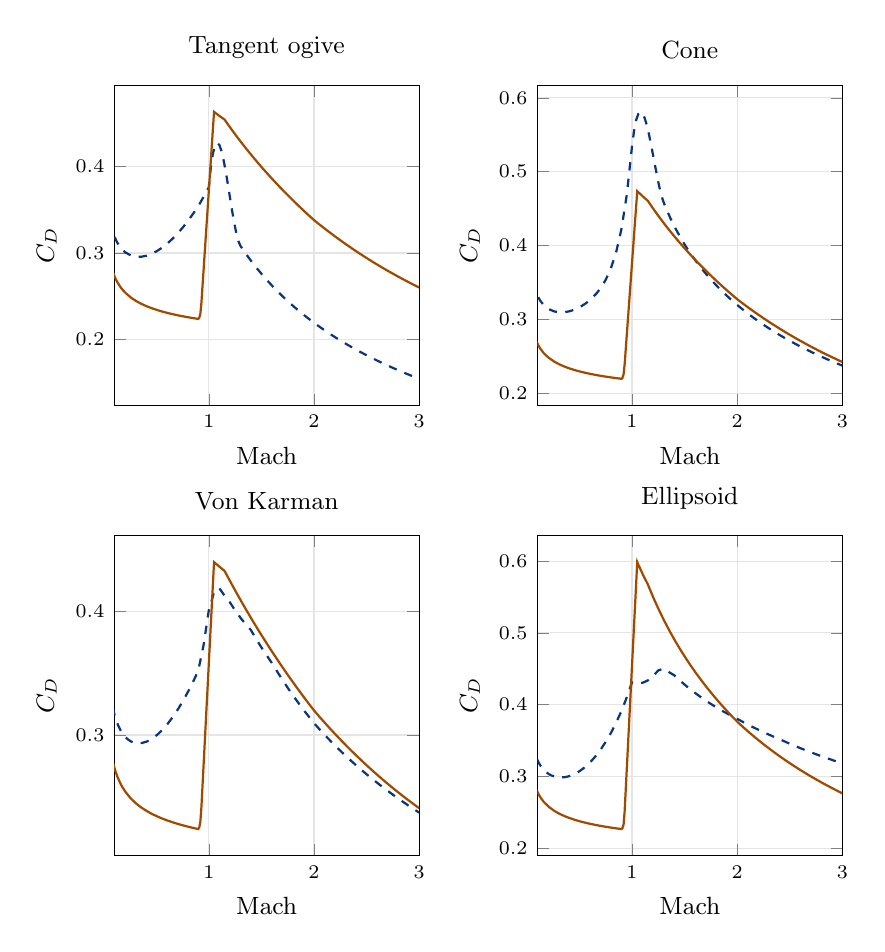
\begin{tikzpicture}
\begin{groupplot}[group style={group size=2 by 2,horizontal sep=1.50cm,vertical sep=1.65cm},width=.45\textwidth,height=5.65cm,grid=major,grid style={gray!20},tick label style={font=\scriptsize},label style={font=\small},title style={font=\small},scaled y ticks=false,yticklabel style={/pgf/number format/fixed,/pgf/number format/precision=3},unbounded coords=jump]
\nextgroupplot[title={Tangent ogive},xlabel={Mach},ylabel={$C_D$},xmin=0.1,xmax=3]
\addplot[thick,B,dashed] coordinates {(0.01,0.432385) (0.02,0.3897077) (0.03,0.368739) (0.04,0.355364) (0.05,0.3457716) (0.06,0.3384154) (0.07,0.3325257) (0.08,0.3276676) (0.09,0.3235729) (0.11,0.3170244) (0.13,0.312015) (0.16,0.3064266) (0.18,0.303622) (0.21,0.3004307) (0.26,0.2971293) (0.31,0.2956987) (0.36,0.2957129) (0.41,0.296925) (0.46,0.29918) (0.51,0.3023746) (0.56,0.3064369) (0.61,0.311315) (0.66,0.3169702) (0.71,0.3233731) (0.76,0.3305008) (0.81,0.3383351) (0.86,0.3468615) (0.91,0.3561867) (0.96,0.3667604) (1,0.3758332) (1.01,0.3876035) (1.02,0.3994312) (1.04,0.41525) (1.06,0.4241697) (1.08,0.4270714) (1.1,0.424837) (1.11,0.4213711) (1.12,0.4179431) (1.14,0.4076398) (1.16,0.3948092) (1.18,0.3803337) (1.21,0.3575234) (1.22,0.34998) (1.24,0.3358689) (1.26,0.323647) (1.28,0.3141988) (1.3,0.308409) (1.31,0.3065889) (1.36,0.2978366) (1.41,0.2896227) (1.46,0.2818902) (1.51,0.2745922) (1.56,0.2676872) (1.61,0.2611402) (1.66,0.2549197) (1.71,0.2489988) (1.76,0.2433533) (1.81,0.2379621) (1.86,0.2328059) (1.91,0.2278679) (1.96,0.2231329) (2.01,0.2185872) (2.06,0.2142184) (2.11,0.2100153) (2.16,0.2059678) (2.21,0.2020666) (2.26,0.1983031) (2.31,0.1946698) (2.36,0.1911594) (2.41,0.1877654) (2.46,0.1844817) (2.51,0.1813028) (2.56,0.1782235) (2.61,0.175239) (2.66,0.1723447) (2.71,0.1695367) (2.76,0.1668109) (2.81,0.1641637) (2.86,0.1615918) (2.91,0.1590919) (2.96,0.156661) (3,0.154764)};
\addplot[thick,burntorange] coordinates {(0.01,0.3747526) (0.02,0.3370981) (0.03,0.3184175) (0.04,0.3064439) (0.05,0.2978187) (0.06,0.2911705) (0.07,0.2858134) (0.08,0.2813592) (0.09,0.2775679) (0.11,0.2713925) (0.13,0.2665116) (0.16,0.2607559) (0.18,0.2576371) (0.21,0.2537077) (0.26,0.2485362) (0.31,0.2445031) (0.36,0.2412271) (0.41,0.238487) (0.46,0.2361445) (0.51,0.2341071) (0.56,0.2323107) (0.61,0.2307088) (0.66,0.2292669) (0.71,0.2279585) (0.76,0.2267632) (0.81,0.2256647) (0.86,0.2246499) (0.9,0.2238911) (0.91,0.2254135) (0.92,0.2299809) (0.93,0.2425879) (0.96,0.2976764) (1.01,0.3894907) (1.05,0.4629422) (1.06,0.4619899) (1.11,0.4574285) (1.15,0.4539954) (1.16,0.4522726) (1.21,0.4436996) (1.26,0.4354433) (1.31,0.4274746) (1.36,0.4197684) (1.41,0.412304) (1.46,0.4050635) (1.51,0.3980314) (1.56,0.3911943) (1.61,0.3845406) (1.66,0.3780599) (1.71,0.371743) (1.76,0.3655817) (1.81,0.3595688) (1.86,0.3536978) (1.91,0.3479626) (1.96,0.3423577) (2.01,0.336981) (2.06,0.3321207) (2.11,0.3273803) (2.16,0.3227565) (2.21,0.3182462) (2.26,0.3138469) (2.31,0.3095557) (2.36,0.3053702) (2.41,0.3012879) (2.46,0.2973064) (2.51,0.2934237) (2.56,0.2896372) (2.61,0.2859449) (2.66,0.2823448) (2.71,0.2788348) (2.76,0.2754128) (2.81,0.2720768) (2.86,0.2688251) (2.91,0.2656555) (2.96,0.2625662) (3,0.2601514)};
\nextgroupplot[title={Cone},xlabel={Mach},ylabel={$C_D$},xmin=0.1,xmax=3]
\addplot[thick,B,dashed] coordinates {(0.01,0.4410384) (0.02,0.3999209) (0.03,0.3797202) (0.04,0.3668369) (0.05,0.357599) (0.06,0.3505166) (0.07,0.3448482) (0.08,0.3401745) (0.09,0.3362374) (0.11,0.329947) (0.13,0.3251433) (0.16,0.3198003) (0.18,0.3171304) (0.21,0.3141112) (0.26,0.3110424) (0.31,0.3098016) (0.36,0.3099828) (0.41,0.3113592) (0.46,0.3138082) (0.51,0.3172864) (0.56,0.3218352) (0.61,0.3276084) (0.66,0.3349257) (0.7,0.3420819) (0.71,0.3443558) (0.75,0.3537388) (0.76,0.3568391) (0.8,0.3695206) (0.81,0.3738582) (0.85,0.3914841) (0.86,0.3976725) (0.9,0.422697) (0.91,0.4317431) (0.95,0.4682605) (0.96,0.4813555) (1,0.5340751) (1.01,0.5447368) (1.02,0.5554556) (1.04,0.5699144) (1.06,0.5781893) (1.08,0.5810194) (1.1,0.5791442) (1.11,0.5760096) (1.12,0.5729129) (1.14,0.5634201) (1.16,0.5514055) (1.18,0.5376095) (1.21,0.51519) (1.24,0.4929422) (1.26,0.4794319) (1.28,0.4678478) (1.3,0.4589325) (1.31,0.4553664) (1.36,0.4387564) (1.41,0.424201) (1.46,0.4111389) (1.51,0.3993363) (1.56,0.3885158) (1.61,0.3785604) (1.66,0.3693104) (1.71,0.3606981) (1.76,0.3526218) (1.81,0.3450387) (1.86,0.3378791) (1.91,0.3311141) (1.96,0.3246936) (2.01,0.3185969) (2.06,0.3127865) (2.11,0.3072473) (2.16,0.3019502) (2.21,0.2968839) (2.26,0.2920254) (2.31,0.2873657) (2.36,0.2828864) (2.41,0.2785804) (2.46,0.2744327) (2.51,0.2704374) (2.56,0.2665821) (2.61,0.2628619) (2.66,0.2592664) (2.71,0.2557917) (2.76,0.2524287) (2.81,0.2491742) (2.86,0.2460206) (2.91,0.2429649) (2.96,0.2400005) (3,0.237693)};
\addplot[thick,burntorange] coordinates {(0.01,0.3638861) (0.02,0.3278052) (0.03,0.3099244) (0.04,0.2984721) (0.05,0.2902274) (0.06,0.2838757) (0.07,0.2787598) (0.08,0.2745079) (0.09,0.2708901) (0.11,0.265) (0.13,0.2603474) (0.16,0.2548643) (0.18,0.2518948) (0.21,0.2481555) (0.26,0.2432376) (0.31,0.2394053) (0.36,0.2362945) (0.41,0.2336943) (0.46,0.2314726) (0.51,0.2295414) (0.56,0.2278393) (0.61,0.2263223) (0.66,0.2249573) (0.71,0.2237193) (0.76,0.2225887) (0.81,0.22155) (0.86,0.2205908) (0.9,0.2198738) (0.91,0.2213689) (0.92,0.2258544) (0.93,0.2389993) (0.96,0.2976847) (1.01,0.3954936) (1.05,0.4737407) (1.06,0.4723418) (1.11,0.4656795) (1.15,0.4607096) (1.16,0.4586207) (1.21,0.4483168) (1.26,0.4384802) (1.31,0.4290633) (1.36,0.420026) (1.41,0.4113343) (1.46,0.402959) (1.51,0.3948751) (1.56,0.3870607) (1.61,0.379497) (1.66,0.3721671) (1.71,0.3650565) (1.76,0.3581519) (1.81,0.3514417) (1.86,0.3449155) (1.91,0.3385638) (1.96,0.332378) (2.01,0.3264494) (2.06,0.3210532) (2.11,0.3158047) (2.16,0.3106988) (2.21,0.3057305) (2.26,0.3008954) (2.31,0.2961893) (2.36,0.2916083) (2.41,0.2871485) (2.46,0.2828065) (2.51,0.278579) (2.56,0.2744626) (2.61,0.2704544) (2.66,0.2665514) (2.71,0.2627508) (2.76,0.2590498) (2.81,0.2554457) (2.86,0.2519362) (2.91,0.2485185) (2.96,0.2451903) (3,0.2425907)};
\nextgroupplot[title={Von Karman},xlabel={Mach},ylabel={$C_D$},xmin=0.1,xmax=3]
\addplot[thick,B,dashed] coordinates {(0.01,0.4294374) (0.02,0.3869424) (0.03,0.3660635) (0.04,0.352746) (0.05,0.3431949) (0.06,0.3358708) (0.07,0.3300069) (0.08,0.3251704) (0.09,0.3210941) (0.1,0.3176028) (0.11,0.3145758) (0.13,0.3095904) (0.14,0.3075196) (0.16,0.3040306) (0.18,0.3012418) (0.21,0.2980706) (0.23,0.2964977) (0.26,0.2947963) (0.28,0.2940383) (0.31,0.2933876) (0.36,0.2934203) (0.41,0.2946486) (0.46,0.2969181) (0.51,0.300126) (0.56,0.3042007) (0.61,0.3090904) (0.66,0.3147567) (0.71,0.3211703) (0.76,0.3283083) (0.81,0.3361527) (0.86,0.3446891) (0.9,0.3520083) (0.91,0.3560236) (0.95,0.3724203) (0.96,0.378004) (1,0.4006815) (1.01,0.4035491) (1.05,0.4155819) (1.06,0.4161249) (1.1,0.4188057) (1.11,0.4175011) (1.16,0.4115277) (1.2,0.4073542) (1.21,0.4059881) (1.26,0.3995847) (1.31,0.393835) (1.36,0.3886687) (1.4,0.3849149) (1.41,0.3834256) (1.46,0.3762536) (1.51,0.3695078) (1.56,0.363149) (1.61,0.356893) (1.66,0.3499598) (1.71,0.3433226) (1.76,0.3369581) (1.81,0.3308454) (1.86,0.3249657) (1.91,0.3193025) (1.96,0.3138406) (2.01,0.3086367) (2.06,0.3038884) (2.11,0.2993047) (2.16,0.2948756) (2.21,0.2905919) (2.26,0.2864452) (2.31,0.2824277) (2.36,0.2785325) (2.41,0.2747531) (2.46,0.2710835) (2.51,0.267518) (2.56,0.2640516) (2.61,0.2606796) (2.66,0.2573974) (2.71,0.2542009) (2.76,0.2510863) (2.81,0.2480499) (2.86,0.2450885) (2.91,0.2421987) (2.96,0.2393776) (3,0.2371683)};
\addplot[thick,burntorange] coordinates {(0.01,0.3747526) (0.02,0.3370981) (0.03,0.3184175) (0.04,0.3064439) (0.05,0.2978187) (0.06,0.2911705) (0.07,0.2858134) (0.08,0.2813592) (0.09,0.2775679) (0.11,0.2713925) (0.13,0.2665116) (0.16,0.2607559) (0.18,0.2576371) (0.21,0.2537077) (0.26,0.2485362) (0.31,0.2445031) (0.36,0.2412271) (0.41,0.238487) (0.46,0.2361445) (0.51,0.2341071) (0.56,0.2323107) (0.61,0.2307088) (0.66,0.2292669) (0.71,0.2279585) (0.76,0.2267632) (0.81,0.2256647) (0.86,0.2246499) (0.9,0.2238911) (0.91,0.2254135) (0.92,0.2299809) (0.93,0.2416627) (0.96,0.2912005) (1.01,0.3737635) (1.05,0.4398139) (1.06,0.4390799) (1.11,0.4354857) (1.15,0.4326966) (1.16,0.4311192) (1.21,0.4231911) (1.26,0.4154615) (1.31,0.4079222) (1.36,0.400565) (1.41,0.3933827) (1.46,0.3863683) (1.51,0.3795156) (1.56,0.3728185) (1.61,0.3662717) (1.66,0.3598698) (1.71,0.3536081) (1.76,0.3474819) (1.81,0.3414869) (1.86,0.3356194) (1.91,0.3298753) (1.96,0.3242509) (2.01,0.3188459) (2.06,0.3139498) (2.11,0.309167) (2.16,0.3044955) (2.21,0.299933) (2.26,0.2954776) (2.31,0.2911272) (2.36,0.2868799) (2.41,0.2827336) (2.46,0.2786864) (2.51,0.2747365) (2.56,0.2708818) (2.61,0.2671206) (2.66,0.2634509) (2.71,0.259871) (2.76,0.2563789) (2.81,0.2529728) (2.86,0.249651) (2.91,0.2464116) (2.96,0.2432528) (3,0.2407826)};
\nextgroupplot[title={Ellipsoid},xlabel={Mach},ylabel={$C_D$},xmin=0.1,xmax=3]
\addplot[thick,B,dashed] coordinates {(0.01,0.4385464) (0.02,0.3947994) (0.03,0.373304) (0.04,0.3595919) (0.05,0.3497564) (0.06,0.3422136) (0.07,0.3361734) (0.08,0.3311899) (0.09,0.3269883) (0.1,0.3233882) (0.11,0.3202689) (0.12,0.3175376) (0.13,0.3151284) (0.14,0.3129913) (0.16,0.3093947) (0.18,0.306524) (0.21,0.3032679) (0.23,0.3016692) (0.26,0.2999644) (0.29,0.29898) (0.31,0.2986786) (0.32,0.2986316) (0.36,0.2990205) (0.39,0.2999172) (0.41,0.3007909) (0.44,0.3024932) (0.46,0.3038923) (0.49,0.3063723) (0.51,0.3082877) (0.54,0.3115431) (0.56,0.3139794) (0.59,0.3180254) (0.61,0.3209976) (0.64,0.3258625) (0.66,0.3293932) (0.7,0.3370824) (0.71,0.3392337) (0.75,0.3481279) (0.76,0.3506005) (0.8,0.3607728) (0.81,0.3635869) (0.85,0.3751192) (0.86,0.3782968) (0.9,0.3912789) (0.91,0.3949657) (0.95,0.4100509) (0.96,0.4141874) (1,0.4310783) (1.01,0.430609) (1.05,0.4292967) (1.06,0.4294438) (1.09,0.4301937) (1.11,0.4311101) (1.15,0.4337462) (1.16,0.4348976) (1.2,0.4398283) (1.21,0.441352) (1.25,0.4477344) (1.26,0.4481985) (1.3,0.4503104) (1.31,0.4492995) (1.36,0.4445846) (1.4,0.4411925) (1.41,0.4397936) (1.46,0.4330745) (1.51,0.4267823) (1.56,0.4208779) (1.61,0.4153019) (1.66,0.4099493) (1.71,0.4048935) (1.76,0.400111) (1.81,0.3955809) (1.86,0.3912845) (1.91,0.3872052) (1.96,0.3833279) (2.01,0.3795392) (2.06,0.3755268) (2.11,0.3716797) (2.16,0.3679877) (2.21,0.3644417) (2.26,0.3610333) (2.31,0.3577549) (2.36,0.3545993) (2.41,0.3514851) (2.46,0.3481813) (2.51,0.3449822) (2.56,0.3418829) (2.61,0.3388784) (2.66,0.3359643) (2.71,0.3331366) (2.76,0.3303913) (2.81,0.3277248) (2.86,0.3251337) (2.91,0.3226148) (2.96,0.3201652) (3,0.3182534)};
\addplot[thick,burntorange] coordinates {(0.01,0.3822419) (0.02,0.3435093) (0.03,0.324281) (0.04,0.3119504) (0.05,0.3030647) (0.06,0.2962135) (0.07,0.2906913) (0.08,0.2860986) (0.09,0.2821886) (0.11,0.2758179) (0.13,0.2707808) (0.16,0.2648387) (0.21,0.2575583) (0.26,0.2522135) (0.31,0.2480431) (0.36,0.2446541) (0.41,0.2418185) (0.46,0.2393934) (0.51,0.2372836) (0.56,0.2354227) (0.61,0.2337628) (0.66,0.2322683) (0.71,0.2309119) (0.76,0.2296724) (0.81,0.228533) (0.86,0.2274802) (0.9,0.2266928) (0.91,0.2282343) (0.92,0.2328588) (0.93,0.2508214) (0.96,0.3377865) (1.01,0.4827283) (1.05,0.5986818) (1.06,0.5952638) (1.11,0.5793348) (1.15,0.5678301) (1.16,0.5642155) (1.21,0.5468583) (1.26,0.5308157) (1.31,0.5159109) (1.36,0.5019975) (1.41,0.4889545) (1.46,0.4766805) (1.51,0.4650899) (1.56,0.4541101) (1.61,0.4436796) (1.66,0.4337452) (1.71,0.424261) (1.76,0.4151872) (1.81,0.4064893) (1.86,0.3981371) (1.91,0.3901037) (1.96,0.3823657) (2.01,0.3750074) (2.06,0.3683105) (2.11,0.3618562) (2.16,0.3556302) (2.21,0.3496199) (2.26,0.3438136) (2.31,0.338201) (2.36,0.3327727) (2.41,0.3275196) (2.46,0.322434) (2.51,0.3175086) (2.56,0.3127362) (2.61,0.3081108) (2.66,0.3036263) (2.71,0.2992774) (2.76,0.2950587) (2.81,0.2909654) (2.86,0.2869931) (2.91,0.2831372) (2.96,0.2793937) (3,0.2764772)};
\end{groupplot}\end{tikzpicture}
\caption{Finless 4 in body, overall length 60 in, nose length 12 in. Body length changes to hold total length fixed.}\label{fig:atlas-04-noses-L12}
\end{figure}
\noindent{\footnotesize Export files: \code{04-noses-L12.svg} and \code{04-noses-L12.png}.\\ Directory: \code{aerodynamic-investigation/extended/figures/}.}

\clearpage\subsubsection*{Nose shapes at L/D = 4.5}
\begin{figure}[H]\centering
{\footnotesize\begin{tabular}{ll}
\tikz[baseline=-.5ex]{\draw[thick,B,dashed] (0,0)--(.40,0);}\ MIT OR & \tikz[baseline=-.5ex]{\draw[thick,burntorange] (0,0)--(.40,0);}\ RASAero\\
\end{tabular}}\par\vspace{.7em}
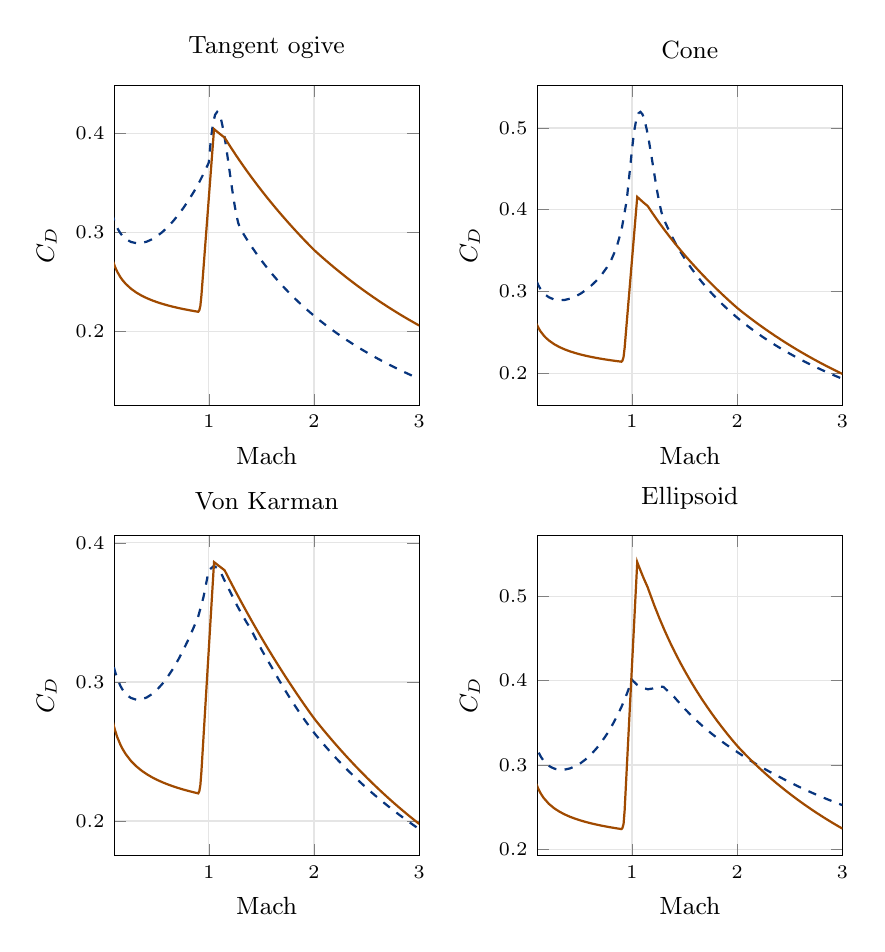
\begin{tikzpicture}
\begin{groupplot}[group style={group size=2 by 2,horizontal sep=1.50cm,vertical sep=1.65cm},width=.45\textwidth,height=5.65cm,grid=major,grid style={gray!20},tick label style={font=\scriptsize},label style={font=\small},title style={font=\small},scaled y ticks=false,yticklabel style={/pgf/number format/fixed,/pgf/number format/precision=3},unbounded coords=jump]
\nextgroupplot[title={Tangent ogive},xlabel={Mach},ylabel={$C_D$},xmin=0.1,xmax=3]
\addplot[thick,B,dashed] coordinates {(0.01,0.4205458) (0.02,0.379424) (0.03,0.3592211) (0.04,0.3463365) (0.05,0.3370976) (0.06,0.3300145) (0.07,0.3243454) (0.08,0.3196712) (0.09,0.3157337) (0.11,0.3094426) (0.13,0.3046383) (0.16,0.2992946) (0.18,0.2966243) (0.21,0.2936046) (0.26,0.2905346) (0.31,0.289291) (0.36,0.2894632) (0.41,0.2908135) (0.46,0.2931923) (0.51,0.2965001) (0.56,0.3006678) (0.61,0.3056452) (0.66,0.311395) (0.71,0.317889) (0.76,0.3251051) (0.81,0.3330257) (0.86,0.3416369) (0.91,0.3510415) (0.96,0.3616728) (1,0.3707863) (1.01,0.3825707) (1.02,0.3944124) (1.04,0.4102591) (1.06,0.4192067) (1.08,0.4221358) (1.1,0.4199282) (1.11,0.4164827) (1.12,0.413075) (1.14,0.4028127) (1.16,0.3900232) (1.18,0.3755887) (1.21,0.3528394) (1.22,0.3453161) (1.24,0.3312448) (1.26,0.3190619) (1.28,0.3096517) (1.3,0.3038988) (1.31,0.3020965) (1.36,0.2934301) (1.41,0.2852962) (1.46,0.2776395) (1.51,0.2704139) (1.56,0.2635784) (1.61,0.2570985) (1.66,0.250943) (1.71,0.2450853) (1.76,0.2395012) (1.81,0.2341697) (1.86,0.229072) (1.91,0.2241911) (1.96,0.2195118) (2.01,0.2150207) (2.06,0.2107053) (2.11,0.2065545) (2.16,0.2025582) (2.21,0.1987072) (2.26,0.1949929) (2.31,0.1914077) (2.36,0.1879445) (2.41,0.1845968) (2.46,0.1813585) (2.51,0.1782241) (2.56,0.1751884) (2.61,0.1722467) (2.66,0.1693944) (2.71,0.1666274) (2.76,0.163942) (2.81,0.1613344) (2.86,0.1588012) (2.91,0.1563393) (2.96,0.1539457) (3,0.1520781)};
\addplot[thick,burntorange] coordinates {(0.01,0.3639171) (0.02,0.3278318) (0.03,0.3099487) (0.04,0.2984948) (0.05,0.2902491) (0.06,0.2838965) (0.07,0.27878) (0.08,0.2745274) (0.09,0.2709091) (0.11,0.2650182) (0.13,0.2603649) (0.16,0.2548811) (0.18,0.2519112) (0.21,0.2481713) (0.26,0.2432527) (0.31,0.2394198) (0.36,0.2363085) (0.41,0.233708) (0.46,0.2314859) (0.51,0.2295543) (0.56,0.227852) (0.61,0.2263347) (0.66,0.2249695) (0.71,0.2237313) (0.76,0.2226005) (0.81,0.2215617) (0.86,0.2206023) (0.9,0.2198852) (0.91,0.2213804) (0.92,0.2258661) (0.93,0.2362482) (0.96,0.2783559) (1.01,0.3485353) (1.05,0.4046789) (1.06,0.4037704) (1.11,0.3994195) (1.15,0.3961459) (1.16,0.3944618) (1.21,0.3860761) (1.26,0.3779974) (1.31,0.3701975) (1.36,0.3626524) (1.41,0.3553421) (1.46,0.3482493) (1.51,0.3413591) (1.56,0.3346587) (1.61,0.3281369) (1.66,0.3217836) (1.71,0.3155901) (1.76,0.3095486) (1.81,0.303652) (1.86,0.297894) (1.91,0.2922688) (1.96,0.2867712) (2.01,0.2814954) (2.06,0.2767193) (2.11,0.2720605) (2.16,0.2675162) (2.21,0.2630832) (2.26,0.258759) (2.31,0.2545411) (2.36,0.2504269) (2.41,0.246414) (2.46,0.2425003) (2.51,0.2386835) (2.56,0.2349613) (2.61,0.2313318) (2.66,0.2277928) (2.71,0.2243425) (2.76,0.2209789) (2.81,0.2176998) (2.86,0.2145036) (2.91,0.2113882) (2.96,0.2083519) (3,0.2059786)};
\nextgroupplot[title={Cone},xlabel={Mach},ylabel={$C_D$},xmin=0.1,xmax=3]
\addplot[thick,B,dashed] coordinates {(0.01,0.4124132) (0.02,0.3735995) (0.03,0.3545332) (0.04,0.3423762) (0.05,0.3336619) (0.06,0.326984) (0.07,0.3216423) (0.08,0.3172412) (0.09,0.3135369) (0.11,0.3076277) (0.13,0.3031278) (0.16,0.2981471) (0.18,0.2956762) (0.21,0.2929111) (0.26,0.2901846) (0.31,0.2892185) (0.36,0.2896254) (0.41,0.2911811) (0.46,0.2937461) (0.51,0.2972314) (0.56,0.3015863) (0.61,0.3068034) (0.66,0.3129475) (0.71,0.3202244) (0.76,0.3291221) (0.8,0.337774) (0.81,0.3406813) (0.85,0.3525844) (0.86,0.3569847) (0.9,0.3748558) (0.91,0.3821188) (0.95,0.4114999) (0.96,0.4238145) (1,0.4734086) (1.01,0.4843763) (1.02,0.4954007) (1.04,0.5098993) (1.06,0.5177334) (1.08,0.5197326) (1.1,0.5167276) (1.11,0.512935) (1.12,0.5091802) (1.14,0.4982563) (1.16,0.4847864) (1.18,0.4696019) (1.21,0.4454609) (1.24,0.4220803) (1.26,0.4083589) (1.28,0.3970855) (1.3,0.3890937) (1.31,0.3861286) (1.36,0.3722332) (1.41,0.359888) (1.46,0.348699) (1.51,0.3384944) (1.56,0.329075) (1.61,0.320351) (1.66,0.3122053) (1.71,0.3045837) (1.76,0.2974102) (1.81,0.2906493) (1.86,0.2842478) (1.91,0.2781811) (1.96,0.2724104) (2.01,0.2669175) (2.06,0.2616733) (2.11,0.2566638) (2.16,0.2518663) (2.21,0.2472702) (2.26,0.2428572) (2.31,0.2386189) (2.36,0.2345406) (2.41,0.2306154) (2.46,0.2268311) (2.51,0.2231822) (2.56,0.2196585) (2.61,0.2162552) (2.66,0.212964) (2.71,0.2097807) (2.76,0.2066982) (2.81,0.203713) (2.86,0.200819) (2.91,0.198013) (2.96,0.1952899) (3,0.1931691)};
\addplot[thick,burntorange] coordinates {(0.01,0.3479405) (0.02,0.3141912) (0.03,0.297496) (0.04,0.2868166) (0.05,0.2791364) (0.06,0.2732246) (0.07,0.2684667) (0.08,0.264515) (0.09,0.2611547) (0.11,0.2556884) (0.13,0.2513747) (0.16,0.2462965) (0.18,0.243549) (0.21,0.2400921) (0.26,0.2355512) (0.31,0.2320174) (0.36,0.2291524) (0.41,0.2267602) (0.46,0.2247182) (0.51,0.2229448) (0.56,0.2213832) (0.61,0.2199925) (0.66,0.2187421) (0.71,0.2176088) (0.76,0.2165745) (0.81,0.215625) (0.86,0.2147486) (0.9,0.2140939) (0.91,0.2155497) (0.92,0.2199172) (0.93,0.2308927) (0.96,0.2770914) (1.01,0.3540894) (1.05,0.4156877) (1.06,0.4144776) (1.11,0.4087131) (1.15,0.4044115) (1.16,0.4024834) (1.21,0.3929481) (1.26,0.3838267) (1.31,0.3750777) (1.36,0.3666659) (1.41,0.358562) (1.46,0.3507404) (1.51,0.3431795) (1.56,0.3358602) (1.61,0.3287664) (1.66,0.3218834) (1.71,0.3151985) (1.76,0.3087003) (1.81,0.3023786) (1.86,0.2962247) (1.91,0.29023) (1.96,0.2843873) (2.01,0.2787832) (2.06,0.2736781) (2.11,0.2687093) (2.16,0.2638724) (2.21,0.259163) (2.26,0.2545773) (2.31,0.2501117) (2.36,0.2457628) (2.41,0.2415271) (2.46,0.2374017) (2.51,0.2333836) (2.56,0.2294697) (2.61,0.2256577) (2.66,0.2219446) (2.71,0.2183281) (2.76,0.2148056) (2.81,0.2113748) (2.86,0.2080333) (2.91,0.2047788) (2.96,0.2016092) (3,0.1991331)};
\nextgroupplot[title={Von Karman},xlabel={Mach},ylabel={$C_D$},xmin=0.1,xmax=3]
\addplot[thick,B,dashed] coordinates {(0.01,0.4177076) (0.02,0.376825) (0.03,0.35674) (0.04,0.3439308) (0.05,0.3347463) (0.06,0.3277051) (0.07,0.32207) (0.08,0.3174242) (0.09,0.3135108) (0.1,0.3101613) (0.11,0.3072593) (0.13,0.3024866) (0.16,0.2971805) (0.18,0.2945309) (0.21,0.2915375) (0.23,0.2900676) (0.26,0.2885032) (0.31,0.2872883) (0.36,0.2874849) (0.41,0.2888564) (0.46,0.2912542) (0.51,0.2945795) (0.56,0.2987633) (0.61,0.303756) (0.66,0.3095204) (0.71,0.3160285) (0.76,0.3232581) (0.81,0.331192) (0.86,0.3398163) (0.9,0.347205) (0.91,0.3499183) (0.95,0.3611045) (0.96,0.364924) (1,0.3805416) (1.01,0.381018) (1.05,0.3834824) (1.06,0.3828947) (1.1,0.3810487) (1.11,0.3793389) (1.16,0.3713386) (1.21,0.3639223) (1.26,0.3562473) (1.31,0.3492249) (1.36,0.3427849) (1.4,0.3380115) (1.41,0.3364741) (1.46,0.3290615) (1.51,0.3220741) (1.56,0.3154729) (1.61,0.309068) (1.66,0.3023621) (1.71,0.2959514) (1.76,0.2898126) (1.81,0.2839246) (1.86,0.2782689) (1.91,0.2728288) (1.96,0.2675893) (2.01,0.2625953) (2.06,0.2580102) (2.11,0.2535888) (2.16,0.2493212) (2.21,0.2451981) (2.26,0.2412113) (2.31,0.2373529) (2.36,0.2336161) (2.41,0.2299942) (2.46,0.2264812) (2.51,0.2230718) (2.56,0.2197606) (2.61,0.216543) (2.66,0.2134145) (2.71,0.2103711) (2.76,0.2074087) (2.81,0.204524) (2.86,0.2017133) (2.91,0.1989737) (2.96,0.1963021) (3,0.194212)};
\addplot[thick,burntorange] coordinates {(0.01,0.3639171) (0.02,0.3278318) (0.03,0.3099487) (0.04,0.2984948) (0.05,0.2902491) (0.06,0.2838965) (0.07,0.27878) (0.08,0.2745274) (0.09,0.2709091) (0.1,0.2677741) (0.11,0.2650182) (0.13,0.2603649) (0.16,0.2548811) (0.18,0.2519112) (0.21,0.2481713) (0.26,0.2432527) (0.31,0.2394198) (0.36,0.2363085) (0.41,0.233708) (0.46,0.2314859) (0.51,0.2295543) (0.56,0.227852) (0.61,0.2263347) (0.66,0.2249695) (0.71,0.2237313) (0.76,0.2226005) (0.81,0.2215617) (0.86,0.2206023) (0.9,0.2198852) (0.91,0.2213804) (0.92,0.2258661) (0.93,0.2355087) (0.96,0.2731792) (1.01,0.3359633) (1.05,0.3861906) (1.06,0.3855972) (1.11,0.3826714) (1.15,0.3803796) (1.16,0.3789216) (1.21,0.3715647) (1.26,0.3643662) (1.31,0.3573222) (1.36,0.3504285) (1.41,0.3436812) (1.46,0.3370764) (1.51,0.33061) (1.56,0.3242784) (1.61,0.318078) (1.66,0.3120052) (1.71,0.3060567) (1.76,0.3002293) (1.81,0.2945197) (1.86,0.2889252) (1.91,0.2834428) (1.96,0.2780697) (2.01,0.2729024) (2.06,0.2682205) (2.11,0.2636435) (2.16,0.2591697) (2.21,0.2547973) (2.26,0.2505251) (2.31,0.2463511) (2.36,0.2422739) (2.41,0.2382917) (2.46,0.2344031) (2.51,0.2306065) (2.56,0.2269) (2.61,0.2232822) (2.66,0.2197513) (2.71,0.2163058) (2.76,0.2129441) (2.81,0.2096644) (2.86,0.2064652) (2.91,0.2033447) (2.96,0.2003015) (3,0.1979214)};
\nextgroupplot[title={Ellipsoid},xlabel={Mach},ylabel={$C_D$},xmin=0.1,xmax=3]
\addplot[thick,B,dashed] coordinates {(0.01,0.4312174) (0.02,0.3884778) (0.03,0.3674784) (0.04,0.3540837) (0.05,0.3444771) (0.06,0.33711) (0.07,0.3312116) (0.08,0.3263462) (0.09,0.3222453) (0.1,0.3187326) (0.11,0.315687) (0.13,0.3106704) (0.14,0.3085862) (0.16,0.305075) (0.18,0.3022686) (0.21,0.2990785) (0.23,0.297499) (0.26,0.2957957) (0.28,0.2950445) (0.31,0.2944143) (0.36,0.2945258) (0.41,0.2959068) (0.46,0.2984325) (0.51,0.3020377) (0.56,0.3066965) (0.61,0.3124118) (0.66,0.3192096) (0.71,0.3271351) (0.76,0.3362511) (0.81,0.3466363) (0.86,0.3583856) (0.9,0.3687663) (0.91,0.3717276) (0.95,0.383909) (0.96,0.3872482) (1,0.4009485) (1.01,0.3996133) (1.05,0.3948356) (1.06,0.3940528) (1.09,0.3920118) (1.11,0.3910146) (1.15,0.3897192) (1.16,0.3898396) (1.2,0.3906461) (1.21,0.391118) (1.25,0.3932927) (1.26,0.3930755) (1.3,0.3924619) (1.31,0.3911965) (1.36,0.385209) (1.4,0.3807983) (1.41,0.3793086) (1.46,0.3721351) (1.51,0.365388) (1.56,0.359028) (1.61,0.3530195) (1.66,0.3473285) (1.71,0.3419338) (1.76,0.3368118) (1.81,0.3319417) (1.86,0.3273048) (1.91,0.3228845) (1.96,0.3186657) (2.01,0.3145732) (2.06,0.3104097) (2.11,0.3064109) (2.16,0.3025668) (2.21,0.2988682) (2.26,0.2953067) (2.31,0.2918747) (2.36,0.288565) (2.41,0.2853327) (2.46,0.2820564) (2.51,0.2788844) (2.56,0.2758115) (2.61,0.2728331) (2.66,0.2699447) (2.71,0.2671421) (2.76,0.2644215) (2.81,0.2617793) (2.86,0.259212) (2.91,0.2567166) (2.96,0.2542899) (3,0.2523962)};
\addplot[thick,burntorange] coordinates {(0.01,0.3752015) (0.02,0.3374822) (0.03,0.3187688) (0.04,0.3067737) (0.05,0.2981329) (0.06,0.2914724) (0.07,0.2861054) (0.08,0.2816429) (0.09,0.2778445) (0.11,0.2716573) (0.13,0.266767) (0.16,0.2610002) (0.21,0.2539379) (0.26,0.2487561) (0.31,0.2447147) (0.36,0.2414319) (0.41,0.2386861) (0.46,0.2363386) (0.51,0.2342969) (0.56,0.2324966) (0.61,0.2308912) (0.66,0.2294461) (0.71,0.2281349) (0.76,0.2269369) (0.81,0.225836) (0.86,0.2248188) (0.9,0.2240583) (0.91,0.2255819) (0.92,0.2301527) (0.93,0.2458507) (0.96,0.3194706) (1.01,0.4421703) (1.05,0.5403301) (1.06,0.5369964) (1.11,0.5214681) (1.15,0.5102617) (1.16,0.5067187) (1.21,0.4897045) (1.26,0.473981) (1.31,0.4593739) (1.36,0.4457395) (1.41,0.4329585) (1.46,0.4209312) (1.51,0.4095737) (1.56,0.3988146) (1.61,0.3885933) (1.66,0.3788578) (1.71,0.3695631) (1.76,0.3606702) (1.81,0.3521452) (1.86,0.3439586) (1.91,0.336084) (1.96,0.3284985) (2.01,0.3212845) (2.06,0.3147173) (2.11,0.3083875) (2.16,0.3022812) (2.21,0.296386) (2.26,0.2906908) (2.31,0.2851852) (2.36,0.27986) (2.41,0.2747066) (2.46,0.2697173) (2.51,0.264885) (2.56,0.2602027) (2.61,0.2556645) (2.66,0.2512644) (2.71,0.2469973) (2.76,0.242858) (2.81,0.2388416) (2.86,0.2349439) (2.91,0.2311605) (2.96,0.2274875) (3,0.2246259)};
\end{groupplot}\end{tikzpicture}
\caption{Finless 4 in body, overall length 60 in, nose length 18 in. Body length changes to hold total length fixed.}\label{fig:atlas-04-noses-L18}
\end{figure}
\noindent{\footnotesize Export files: \code{04-noses-L18.svg} and \code{04-noses-L18.png}.\\ Directory: \code{aerodynamic-investigation/extended/figures/}.}

\clearpage\subsubsection*{Tangent-ogive fineness sweep}
\begin{figure}[H]\centering
{\footnotesize\begin{tabular}{ll}
\tikz[baseline=-.5ex]{\draw[thick,B,dashed] (0,0)--(.40,0);}\ MIT OR & \tikz[baseline=-.5ex]{\draw[thick,burntorange] (0,0)--(.40,0);}\ RASAero\\
\end{tabular}}\par\vspace{.7em}
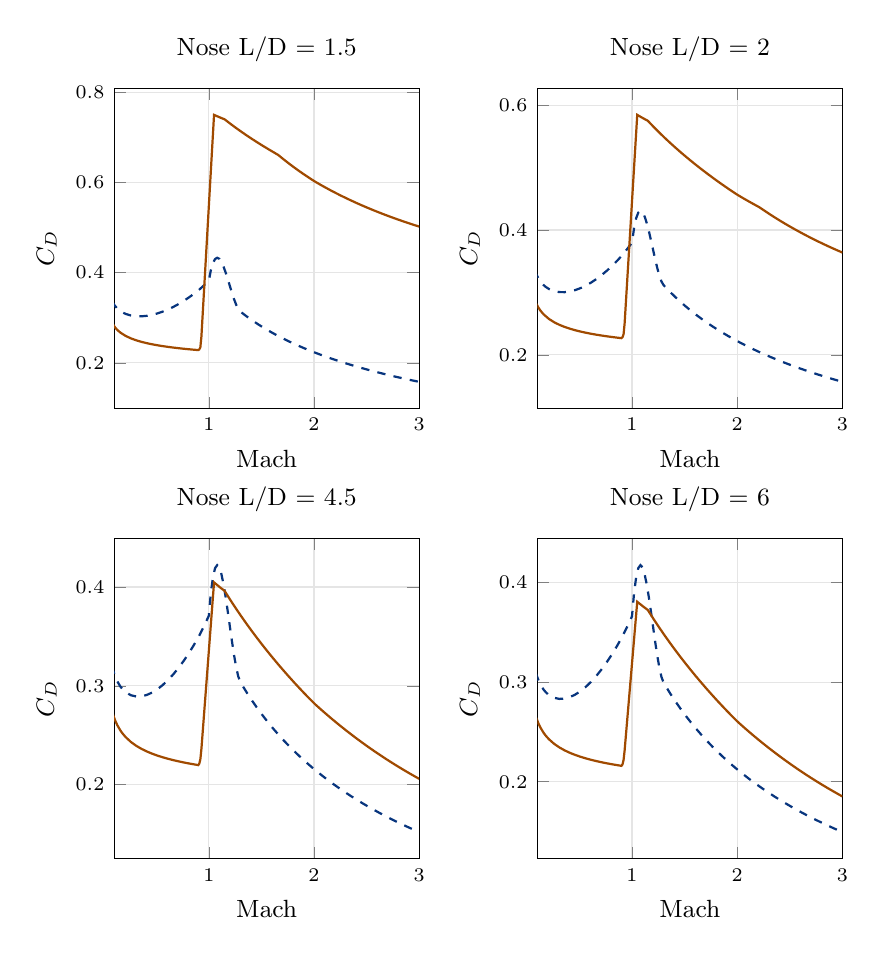
\begin{tikzpicture}
\begin{groupplot}[group style={group size=2 by 2,horizontal sep=1.50cm,vertical sep=1.65cm},width=.45\textwidth,height=5.65cm,grid=major,grid style={gray!20},tick label style={font=\scriptsize},label style={font=\small},title style={font=\small},scaled y ticks=false,yticklabel style={/pgf/number format/fixed,/pgf/number format/precision=3},unbounded coords=jump]
\nextgroupplot[title={Nose L/D = 1.5},xlabel={Mach},ylabel={$C_D$},xmin=0.1,xmax=3]
\addplot[thick,B,dashed] coordinates {(0.01,0.4455416) (0.02,0.4012453) (0.03,0.3794793) (0.04,0.365594) (0.05,0.3556335) (0.06,0.3479931) (0.07,0.3418738) (0.08,0.3368241) (0.09,0.3325658) (0.11,0.3257494) (0.13,0.3205265) (0.16,0.3146834) (0.18,0.311739) (0.21,0.3083691) (0.26,0.3048268) (0.31,0.3032015) (0.36,0.3030512) (0.41,0.3041195) (0.46,0.3062456) (0.51,0.3093224) (0.56,0.3132751) (0.61,0.3180498) (0.66,0.3236065) (0.71,0.3299145) (0.76,0.3369502) (0.81,0.3446946) (0.86,0.3531328) (0.91,0.3623754) (0.96,0.3728891) (1,0.3819195) (1.01,0.3936675) (1.02,0.4054734) (1.04,0.4212459) (1.06,0.4301177) (1.08,0.4329704) (1.1,0.4306864) (1.11,0.4271879) (1.12,0.4237274) (1.14,0.4133581) (1.16,0.4004608) (1.18,0.3859184) (1.21,0.3630087) (1.22,0.3554325) (1.24,0.3412569) (1.26,0.3289722) (1.28,0.3194633) (1.3,0.3136153) (1.31,0.3117676) (1.36,0.3028855) (1.41,0.2945556) (1.46,0.2867165) (1.51,0.2793199) (1.56,0.2723222) (1.61,0.2656876) (1.66,0.2593837) (1.71,0.2533831) (1.76,0.247661) (1.81,0.2421959) (1.86,0.2369684) (1.91,0.2319614) (1.96,0.2271595) (2.01,0.2225488) (2.06,0.2181168) (2.11,0.2138522) (2.16,0.2097447) (2.21,0.2057851) (2.26,0.2019646) (2.31,0.1982757) (2.36,0.1947109) (2.41,0.1912638) (2.46,0.1879283) (2.51,0.1846987) (2.56,0.1815698) (2.61,0.1785367) (2.66,0.1755951) (2.71,0.1727406) (2.76,0.1699694) (2.81,0.1672777) (2.86,0.1646623) (2.91,0.1621197) (2.96,0.1596471) (3,0.1577174)};
\addplot[thick,burntorange] coordinates {(0.01,0.3860854) (0.02,0.3468013) (0.03,0.3272929) (0.04,0.3147798) (0.05,0.305761) (0.06,0.298806) (0.08,0.2885359) (0.11,0.2780948) (0.13,0.2729779) (0.16,0.2669406) (0.21,0.2595415) (0.26,0.2541081) (0.31,0.2498676) (0.36,0.2464209) (0.41,0.2435365) (0.46,0.2410692) (0.51,0.2389224) (0.56,0.2370286) (0.61,0.2353391) (0.66,0.2338178) (0.71,0.2324368) (0.76,0.2311748) (0.81,0.2300145) (0.86,0.2289423) (0.9,0.2281403) (0.91,0.2296917) (0.92,0.2343458) (0.93,0.2583182) (0.96,0.3812099) (1.01,0.5860293) (1.05,0.7498849) (1.06,0.7488401) (1.11,0.7438373) (1.15,0.7400742) (1.16,0.738272) (1.21,0.7293176) (1.26,0.720705) (1.31,0.7124021) (1.36,0.7043815) (1.41,0.6966204) (1.46,0.689099) (1.51,0.6818004) (1.56,0.67471) (1.61,0.6678149) (1.66,0.6609771) (1.71,0.651455) (1.76,0.6423363) (1.81,0.6335876) (1.86,0.6251795) (1.91,0.6170865) (1.96,0.6092854) (2.01,0.601863) (2.06,0.5951049) (2.11,0.5885878) (2.16,0.582298) (2.21,0.5762228) (2.26,0.5703513) (2.31,0.564673) (2.36,0.5591789) (2.41,0.5538602) (2.46,0.5487092) (2.51,0.5437186) (2.56,0.5388815) (2.61,0.5341919) (2.66,0.529644) (2.71,0.5252321) (2.76,0.5209512) (2.81,0.5167965) (2.86,0.5127635) (2.91,0.5088478) (2.96,0.5050453) (3,0.5020823)};
\nextgroupplot[title={Nose L/D = 2},xlabel={Mach},ylabel={$C_D$},xmin=0.1,xmax=3]
\addplot[thick,B,dashed] coordinates {(0.01,0.4408558) (0.02,0.3971146) (0.03,0.3756221) (0.04,0.3619117) (0.05,0.3520774) (0.06,0.3445345) (0.07,0.3384939) (0.08,0.3335099) (0.09,0.3293078) (0.11,0.3225832) (0.13,0.3174335) (0.16,0.3116777) (0.18,0.3087813) (0.21,0.3054726) (0.26,0.3020129) (0.31,0.3004544) (0.36,0.3003605) (0.41,0.3014781) (0.46,0.3036484) (0.51,0.3067656) (0.56,0.3107559) (0.61,0.315566) (0.66,0.3211565) (0.71,0.3274971) (0.76,0.3345643) (0.81,0.3423395) (0.86,0.350808) (0.91,0.3600789) (0.96,0.3706132) (1,0.3796581) (1.01,0.3914153) (1.02,0.4032303) (1.04,0.4190222) (1.06,0.4279144) (1.08,0.4307881) (1.1,0.4285256) (1.11,0.4250406) (1.12,0.4215936) (1.14,0.4112518) (1.16,0.3983824) (1.18,0.3838679) (1.21,0.3609998) (1.22,0.3534373) (1.24,0.3392886) (1.26,0.32703) (1.28,0.3175463) (1.3,0.3117224) (1.31,0.3098861) (1.36,0.301057) (1.41,0.2927737) (1.46,0.2849769) (1.51,0.277619) (1.56,0.2706573) (1.61,0.2640565) (1.66,0.2577845) (1.71,0.2518142) (1.76,0.246121) (1.81,0.2406836) (1.86,0.2354828) (1.91,0.2305015) (1.96,0.2257243) (2.01,0.2211377) (2.06,0.2167289) (2.11,0.2124869) (2.16,0.2084014) (2.21,0.2044631) (2.26,0.2006634) (2.31,0.1969946) (2.36,0.1934496) (2.41,0.1900217) (2.46,0.186705) (2.51,0.1834937) (2.56,0.1803826) (2.61,0.1773671) (2.66,0.1744425) (2.71,0.1716047) (2.76,0.1688497) (2.81,0.1661741) (2.86,0.1635742) (2.91,0.1610469) (2.96,0.1585892) (3,0.1566712)};
\addplot[thick,burntorange] coordinates {(0.01,0.3821935) (0.02,0.3434678) (0.03,0.324243) (0.04,0.3119147) (0.05,0.3030308) (0.06,0.2961808) (0.07,0.2906597) (0.08,0.2860679) (0.09,0.2821587) (0.11,0.2757892) (0.13,0.2707532) (0.16,0.2648123) (0.21,0.2575334) (0.26,0.2521896) (0.31,0.2480202) (0.36,0.2446319) (0.41,0.2417969) (0.46,0.2393723) (0.51,0.2372629) (0.56,0.2354025) (0.61,0.233743) (0.66,0.2322488) (0.71,0.2308927) (0.76,0.2296535) (0.81,0.2285144) (0.86,0.2274618) (0.9,0.2266746) (0.91,0.228216) (0.92,0.2328401) (0.93,0.250231) (0.96,0.3337673) (1.01,0.4729944) (1.05,0.5843762) (1.06,0.5833743) (1.11,0.5785764) (1.15,0.574966) (1.16,0.5732003) (1.21,0.5644216) (1.26,0.5559724) (1.31,0.5478221) (1.36,0.5399446) (1.41,0.5323181) (1.46,0.5249237) (1.51,0.5177451) (1.56,0.5107682) (1.61,0.5039809) (1.66,0.4973722) (1.71,0.4909325) (1.76,0.4846533) (1.81,0.4785267) (1.86,0.472546) (1.91,0.4667048) (1.96,0.4609974) (2.01,0.455524) (2.06,0.45058) (2.11,0.4457585) (2.16,0.4410565) (2.21,0.4364705) (2.26,0.4307368) (2.31,0.4251751) (2.36,0.4197929) (2.41,0.4145819) (2.46,0.4095345) (2.51,0.4046439) (2.56,0.3999032) (2.61,0.3953065) (2.66,0.3908483) (2.71,0.3865232) (2.76,0.3823261) (2.81,0.3782526) (2.86,0.3742981) (2.91,0.3704585) (2.96,0.3667296) (3,0.3638238)};
\nextgroupplot[title={Nose L/D = 4.5},xlabel={Mach},ylabel={$C_D$},xmin=0.1,xmax=3]
\addplot[thick,B,dashed] coordinates {(0.01,0.4205458) (0.02,0.379424) (0.03,0.3592211) (0.04,0.3463365) (0.05,0.3370976) (0.06,0.3300145) (0.07,0.3243454) (0.08,0.3196712) (0.09,0.3157337) (0.11,0.3094426) (0.13,0.3046383) (0.16,0.2992946) (0.18,0.2966243) (0.21,0.2936046) (0.26,0.2905346) (0.31,0.289291) (0.36,0.2894632) (0.41,0.2908135) (0.46,0.2931923) (0.51,0.2965001) (0.56,0.3006678) (0.61,0.3056452) (0.66,0.311395) (0.71,0.317889) (0.76,0.3251051) (0.81,0.3330257) (0.86,0.3416369) (0.91,0.3510415) (0.96,0.3616728) (1,0.3707863) (1.01,0.3825707) (1.02,0.3944124) (1.04,0.4102591) (1.06,0.4192067) (1.08,0.4221358) (1.1,0.4199282) (1.11,0.4164827) (1.12,0.413075) (1.14,0.4028127) (1.16,0.3900232) (1.18,0.3755887) (1.21,0.3528394) (1.22,0.3453161) (1.24,0.3312448) (1.26,0.3190619) (1.28,0.3096517) (1.3,0.3038988) (1.31,0.3020965) (1.36,0.2934301) (1.41,0.2852962) (1.46,0.2776395) (1.51,0.2704139) (1.56,0.2635784) (1.61,0.2570985) (1.66,0.250943) (1.71,0.2450853) (1.76,0.2395012) (1.81,0.2341697) (1.86,0.229072) (1.91,0.2241911) (1.96,0.2195118) (2.01,0.2150207) (2.06,0.2107053) (2.11,0.2065545) (2.16,0.2025582) (2.21,0.1987072) (2.26,0.1949929) (2.31,0.1914077) (2.36,0.1879445) (2.41,0.1845968) (2.46,0.1813585) (2.51,0.1782241) (2.56,0.1751884) (2.61,0.1722467) (2.66,0.1693944) (2.71,0.1666274) (2.76,0.163942) (2.81,0.1613344) (2.86,0.1588012) (2.91,0.1563393) (2.96,0.1539457) (3,0.1520781)};
\addplot[thick,burntorange] coordinates {(0.01,0.3639171) (0.02,0.3278318) (0.03,0.3099487) (0.04,0.2984948) (0.05,0.2902491) (0.06,0.2838965) (0.07,0.27878) (0.08,0.2745274) (0.09,0.2709091) (0.11,0.2650182) (0.13,0.2603649) (0.16,0.2548811) (0.18,0.2519112) (0.21,0.2481713) (0.26,0.2432527) (0.31,0.2394198) (0.36,0.2363085) (0.41,0.233708) (0.46,0.2314859) (0.51,0.2295543) (0.56,0.227852) (0.61,0.2263347) (0.66,0.2249695) (0.71,0.2237313) (0.76,0.2226005) (0.81,0.2215617) (0.86,0.2206023) (0.9,0.2198852) (0.91,0.2213804) (0.92,0.2258661) (0.93,0.2362482) (0.96,0.2783559) (1.01,0.3485353) (1.05,0.4046789) (1.06,0.4037704) (1.11,0.3994195) (1.15,0.3961459) (1.16,0.3944618) (1.21,0.3860761) (1.26,0.3779974) (1.31,0.3701975) (1.36,0.3626524) (1.41,0.3553421) (1.46,0.3482493) (1.51,0.3413591) (1.56,0.3346587) (1.61,0.3281369) (1.66,0.3217836) (1.71,0.3155901) (1.76,0.3095486) (1.81,0.303652) (1.86,0.297894) (1.91,0.2922688) (1.96,0.2867712) (2.01,0.2814954) (2.06,0.2767193) (2.11,0.2720605) (2.16,0.2675162) (2.21,0.2630832) (2.26,0.258759) (2.31,0.2545411) (2.36,0.2504269) (2.41,0.246414) (2.46,0.2425003) (2.51,0.2386835) (2.56,0.2349613) (2.61,0.2313318) (2.66,0.2277928) (2.71,0.2243425) (2.76,0.2209789) (2.81,0.2176998) (2.86,0.2145036) (2.91,0.2113882) (2.96,0.2083519) (3,0.2059786)};
\nextgroupplot[title={Nose L/D = 6},xlabel={Mach},ylabel={$C_D$},xmin=0.1,xmax=3]
\addplot[thick,B,dashed] coordinates {(0.01,0.4090812) (0.02,0.3694982) (0.03,0.3500531) (0.04,0.3376536) (0.05,0.3287644) (0.06,0.3219515) (0.07,0.3165007) (0.08,0.3120086) (0.09,0.3082265) (0.11,0.30219) (0.13,0.2975887) (0.16,0.292487) (0.18,0.2899496) (0.21,0.2870996) (0.26,0.2842587) (0.31,0.2832) (0.36,0.2835287) (0.41,0.2850155) (0.46,0.2875168) (0.51,0.2909367) (0.56,0.2952086) (0.61,0.3002842) (0.66,0.3061277) (0.71,0.3127119) (0.76,0.3200154) (0.81,0.3280214) (0.86,0.3367165) (0.91,0.3461996) (0.96,0.3568878) (1,0.3660417) (1.01,0.3778379) (1.02,0.3896909) (1.04,0.4055603) (1.06,0.4145297) (1.08,0.4174798) (1.1,0.4152921) (1.11,0.4118632) (1.12,0.4084722) (1.14,0.3982434) (1.16,0.3854872) (1.18,0.371086) (1.21,0.3483861) (1.22,0.3408792) (1.24,0.3268403) (1.26,0.3146893) (1.28,0.3053104) (1.3,0.2995881) (1.31,0.2978008) (1.36,0.2892072) (1.41,0.2811427) (1.46,0.2735528) (1.51,0.2663917) (1.56,0.2596191) (1.61,0.2532002) (1.66,0.2471043) (1.71,0.2413048) (1.76,0.2357777) (1.81,0.230502) (1.86,0.2254589) (1.91,0.2206316) (1.96,0.2160049) (2.01,0.2115653) (2.06,0.2073005) (2.11,0.2031993) (2.16,0.1992517) (2.21,0.1954484) (2.26,0.191781) (2.31,0.1882419) (2.36,0.1848239) (2.41,0.1815205) (2.46,0.1783257) (2.51,0.175234) (2.56,0.1722402) (2.61,0.1693396) (2.66,0.1665277) (2.71,0.1638004) (2.76,0.1611538) (2.81,0.1585843) (2.86,0.1560886) (2.91,0.1536634) (2.96,0.1513058) (3,0.1494666)};
\addplot[thick,burntorange] coordinates {(0.01,0.3532518) (0.02,0.3187227) (0.03,0.3016309) (0.04,0.2906929) (0.05,0.2828238) (0.06,0.2767648) (0.07,0.2718871) (0.08,0.2678349) (0.09,0.2643884) (0.11,0.2587802) (0.13,0.2543531) (0.16,0.2491393) (0.18,0.2463175) (0.21,0.242766) (0.26,0.2380988) (0.31,0.2344651) (0.36,0.2315177) (0.41,0.2290559) (0.46,0.2269536) (0.51,0.2251274) (0.56,0.2235187) (0.61,0.2220856) (0.66,0.2207968) (0.71,0.2196284) (0.76,0.2185619) (0.81,0.2175825) (0.86,0.2166784) (0.9,0.2160027) (0.91,0.2174716) (0.92,0.221878) (0.93,0.2314052) (0.96,0.2687391) (1.01,0.3309622) (1.05,0.3807407) (1.06,0.3798637) (1.11,0.3756657) (1.15,0.3725089) (1.16,0.3708534) (1.21,0.3626063) (1.26,0.3546604) (1.31,0.346988) (1.36,0.3395656) (1.41,0.3323737) (1.46,0.3253953) (1.51,0.3186159) (1.56,0.312023) (1.61,0.3056057) (1.66,0.2993541) (1.71,0.2932597) (1.76,0.2873149) (1.81,0.2815127) (1.86,0.2758472) (1.91,0.2703125) (1.96,0.2649035) (2.01,0.259711) (2.06,0.2550023) (2.11,0.2504094) (2.16,0.2459293) (2.21,0.2415591) (2.26,0.2372963) (2.31,0.2331382) (2.36,0.2290826) (2.41,0.2251269) (2.46,0.2212691) (2.51,0.217507) (2.56,0.2138383) (2.61,0.2102611) (2.66,0.2067733) (2.71,0.2033731) (2.76,0.2000583) (2.81,0.1968271) (2.86,0.1936777) (2.91,0.1906082) (2.96,0.1876167) (3,0.1852786)};
\end{groupplot}\end{tikzpicture}
\caption{Nose length changes at fixed overall length. L/D is nose length divided by body diameter.}\label{fig:atlas-05-ogive-fineness}
\end{figure}
\noindent{\footnotesize Export files: \code{05-ogive-fineness.svg} and \code{05-ogive-fineness.png}.\\ Directory: \code{aerodynamic-investigation/extended/figures/}.}

\clearpage\subsubsection*{Sensitivity to shortening the nose}
\begin{figure}[H]\centering
{\footnotesize\begin{tabular}{ll}
\tikz[baseline=-.5ex]{\draw[thick,B,dashed] (0,0)--(.40,0);}\ MIT OR & \tikz[baseline=-.5ex]{\draw[thick,burntorange] (0,0)--(.40,0);}\ RASAero\\
\end{tabular}}\par\vspace{.7em}
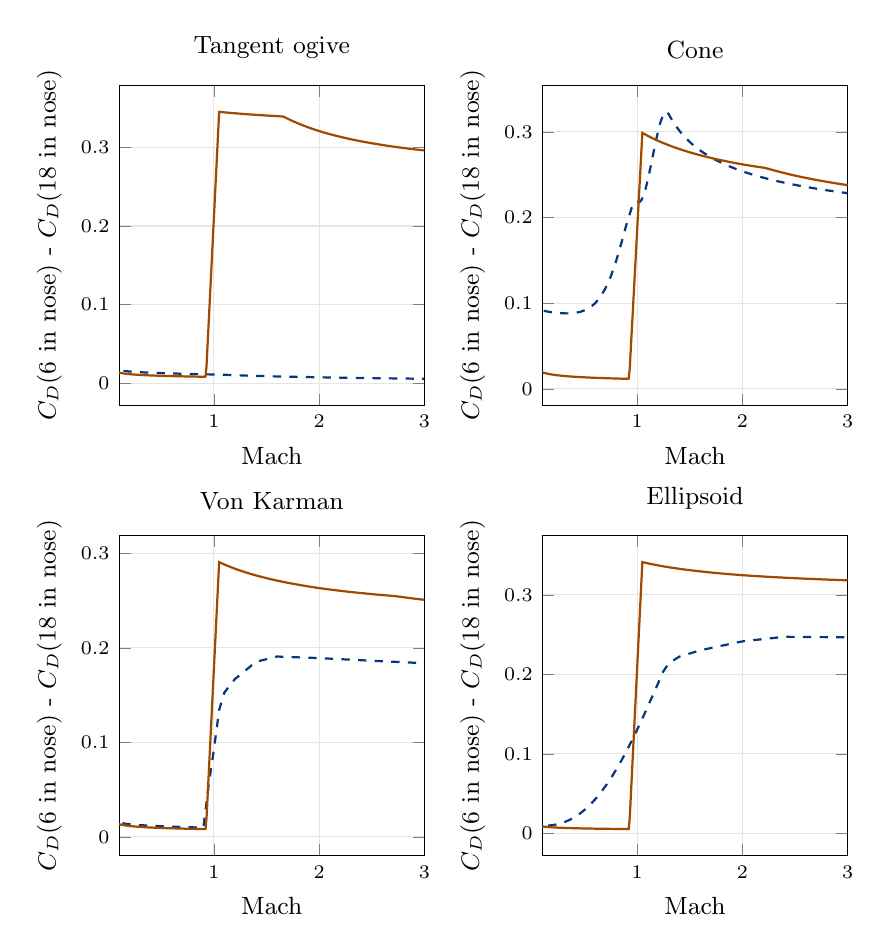
\begin{tikzpicture}
\begin{groupplot}[group style={group size=2 by 2,horizontal sep=1.50cm,vertical sep=1.65cm},width=.45\textwidth,height=5.65cm,grid=major,grid style={gray!20},tick label style={font=\scriptsize},label style={font=\small},title style={font=\small},scaled y ticks=false,yticklabel style={/pgf/number format/fixed,/pgf/number format/precision=3},unbounded coords=jump]
\nextgroupplot[title={Tangent ogive},xlabel={Mach},ylabel={$C_D$(6 in nose) - $C_D$(18 in nose)},xmin=0.1,xmax=3]
\addplot[thick,B,dashed] coordinates {(0.01,0.02499574) (0.02,0.0218213) (0.03,0.02025818) (0.04,0.01925747) (0.05,0.01853591) (0.06,0.01797861) (0.07,0.01752837) (0.08,0.01715284) (0.09,0.01683212) (0.11,0.01630683) (0.13,0.01588819) (0.16,0.01538884) (0.18,0.01511472) (0.21,0.01476453) (0.26,0.01429216) (0.31,0.0139105) (0.36,0.01358792) (0.41,0.01330605) (0.46,0.01305338) (0.51,0.01282223) (0.56,0.01260727) (0.61,0.01240462) (0.66,0.01221142) (0.71,0.01202547) (0.76,0.01184509) (0.81,0.01166891) (0.86,0.01149586) (0.91,0.01133387) (0.96,0.01121636) (1.01,0.0110968) (1.06,0.01091104) (1.11,0.01070527) (1.16,0.0104376) (1.21,0.01016939) (1.26,0.009910301) (1.31,0.009671116) (1.36,0.009455416) (1.41,0.009259355) (1.46,0.009076974) (1.51,0.008906042) (1.56,0.008743766) (1.61,0.008589157) (1.66,0.008440692) (1.71,0.008297878) (1.76,0.008159794) (1.81,0.008026175) (1.86,0.00789642) (1.91,0.007770378) (1.96,0.007647632) (2.01,0.007528093) (2.06,0.00741146) (2.11,0.007297674) (2.16,0.007186509) (2.21,0.007077926) (2.26,0.006971748) (2.31,0.006867947) (2.36,0.006766379) (2.41,0.006667023) (2.46,0.00656976) (2.51,0.00647457) (2.56,0.006381354) (2.61,0.006290094) (2.66,0.006200702) (2.71,0.006113162) (2.76,0.006027397) (2.81,0.00594339) (2.86,0.005861072) (2.91,0.005780427) (2.96,0.005701392) (3,0.005639309)};
\addplot[thick,burntorange] coordinates {(0.01,0.02216825) (0.02,0.01896954) (0.03,0.01734425) (0.06,0.01490949) (0.11,0.01307656) (0.16,0.01205951) (0.21,0.01137026) (0.26,0.01085542) (0.31,0.01044782) (0.36,0.01011238) (0.41,0.009828563) (0.46,0.009583366) (0.51,0.009368076) (0.56,0.00917657) (0.61,0.0090044) (0.66,0.008848237) (0.71,0.008705522) (0.76,0.008574254) (0.81,0.008452841) (0.86,0.008339991) (0.9,0.00825516) (0.91,0.008311295) (0.92,0.0084797) (0.93,0.02207) (0.96,0.102854) (1.01,0.237494) (1.05,0.345206) (1.06,0.3450697) (1.11,0.3444177) (1.16,0.3438101) (1.21,0.3432416) (1.26,0.3427077) (1.31,0.3422046) (1.36,0.3417291) (1.41,0.3412783) (1.46,0.3408497) (1.51,0.3404413) (1.56,0.3400513) (1.61,0.339678) (1.66,0.3391934) (1.71,0.3358649) (1.76,0.3327877) (1.81,0.3299356) (1.86,0.3272855) (1.91,0.3248177) (1.96,0.3225142) (2.01,0.3203676) (2.06,0.3183857) (2.11,0.3165273) (2.16,0.3147818) (2.21,0.3131397) (2.26,0.3115923) (2.31,0.3101319) (2.36,0.308752) (2.41,0.3074462) (2.46,0.3062089) (2.51,0.3050351) (2.56,0.3039202) (2.61,0.3028601) (2.66,0.3018511) (2.71,0.3008895) (2.76,0.2999723) (2.81,0.2990967) (2.86,0.2982599) (2.91,0.2974596) (2.96,0.2966934) (3,0.2961036)};
\nextgroupplot[title={Cone},xlabel={Mach},ylabel={$C_D$(6 in nose) - $C_D$(18 in nose)},xmin=0.1,xmax=3]
\addplot[thick,B,dashed] coordinates {(0.01,0.1040519) (0.02,0.09940461) (0.03,0.09711626) (0.04,0.09565123) (0.06,0.09377917) (0.11,0.09133357) (0.16,0.09000006) (0.21,0.08912413) (0.26,0.0885382) (0.31,0.08822377) (0.35,0.08817757) (0.36,0.08824825) (0.41,0.08875369) (0.46,0.08996038) (0.51,0.09217484) (0.55,0.09478779) (0.56,0.09579704) (0.6,0.09984082) (0.61,0.1013203) (0.65,0.1072434) (0.66,0.1093133) (0.7,0.1175972) (0.71,0.1203655) (0.75,0.1314418) (0.76,0.1349612) (0.8,0.1490413) (0.81,0.1532284) (0.85,0.1699783) (0.86,0.1744674) (0.9,0.192425) (0.91,0.1963309) (0.95,0.2119629) (0.96,0.2134305) (1,0.2193098) (1.01,0.2185857) (1.02,0.2178626) (1.04,0.2201085) (1.06,0.2254674) (1.08,0.2333593) (1.1,0.2432039) (1.11,0.2487904) (1.12,0.2543771) (1.16,0.2785086) (1.18,0.2903063) (1.2,0.3011517) (1.21,0.3058079) (1.22,0.3104644) (1.24,0.3176641) (1.26,0.3221708) (1.28,0.3234039) (1.3,0.3207834) (1.31,0.3185242) (1.34,0.312131) (1.36,0.3083329) (1.41,0.3000627) (1.46,0.2930756) (1.51,0.2871353) (1.56,0.2819435) (1.61,0.2773964) (1.66,0.2733318) (1.71,0.2696982) (1.76,0.2663976) (1.81,0.2634026) (1.86,0.2606493) (1.91,0.2581223) (1.96,0.2557777) (2.01,0.2536066) (2.06,0.2515771) (2.11,0.2496843) (2.16,0.2479044) (2.21,0.2462345) (2.26,0.2446564) (2.31,0.2431684) (2.36,0.2417565) (2.41,0.2404196) (2.46,0.2391465) (2.51,0.2379367) (2.56,0.2367812) (2.61,0.2356797) (2.66,0.2346248) (2.71,0.2336166) (2.76,0.2326486) (2.81,0.2317214) (2.86,0.2308293) (2.91,0.2299729) (2.96,0.2291476) (3,0.2285097)};
\addplot[thick,burntorange] coordinates {(0.01,0.03229119) (0.02,0.02759669) (0.03,0.02521042) (0.04,0.0236548) (0.06,0.02163408) (0.11,0.01894019) (0.16,0.01744468) (0.21,0.01643085) (0.26,0.01567335) (0.31,0.01507351) (0.36,0.01457978) (0.41,0.01416195) (0.46,0.01380093) (0.51,0.0134839) (0.56,0.01320186) (0.61,0.01294828) (0.66,0.01271824) (0.71,0.01250799) (0.76,0.01231459) (0.81,0.0121357) (0.86,0.0119694) (0.9,0.01184439) (0.91,0.01192493) (0.92,0.01216656) (0.93,0.02380776) (0.96,0.09256765) (1.01,0.2071675) (1.05,0.2988473) (1.06,0.2981505) (1.11,0.2948442) (1.16,0.2918056) (1.21,0.2890019) (1.26,0.2864052) (1.31,0.2839923) (1.36,0.281743) (1.41,0.2796399) (1.46,0.2776684) (1.51,0.2758154) (1.56,0.2740697) (1.61,0.2724215) (1.66,0.270862) (1.71,0.2693835) (1.76,0.2679791) (1.81,0.2666431) (1.86,0.2653697) (1.91,0.2641542) (1.96,0.2629923) (2.01,0.2618911) (2.06,0.260879) (2.11,0.2599101) (2.16,0.2589816) (2.21,0.2580908) (2.26,0.2564723) (2.31,0.2547732) (2.36,0.2531582) (2.41,0.2516214) (2.46,0.2501572) (2.51,0.2487607) (2.56,0.2474273) (2.61,0.2461529) (2.66,0.2449336) (2.71,0.2437659) (2.76,0.2426468) (2.81,0.2415732) (2.86,0.2405425) (2.91,0.2395521) (2.96,0.2385997) (3,0.2378638)};
\nextgroupplot[title={Von Karman},xlabel={Mach},ylabel={$C_D$(6 in nose) - $C_D$(18 in nose)},xmin=0.1,xmax=3]
\addplot[thick,B,dashed] coordinates {(0.01,0.0237278) (0.02,0.02046613) (0.03,0.01886008) (0.04,0.01783186) (0.06,0.01651787) (0.11,0.01480016) (0.16,0.01385694) (0.21,0.01321548) (0.26,0.01273012) (0.31,0.01233798) (0.36,0.01200654) (0.41,0.01171693) (0.46,0.01145731) (0.51,0.01121982) (0.56,0.01099894) (0.61,0.01079072) (0.66,0.01059221) (0.71,0.01040116) (0.76,0.01021582) (0.81,0.0100348) (0.86,0.009856999) (0.9,0.009716456) (0.91,0.01872278) (0.95,0.05475389) (0.96,0.06230159) (1,0.09249873) (1.01,0.1008927) (1.05,0.1344754) (1.06,0.1381636) (1.1,0.1529237) (1.11,0.1543339) (1.16,0.1613862) (1.2,0.1670298) (1.21,0.1679453) (1.26,0.1725245) (1.31,0.1771058) (1.36,0.1816891) (1.4,0.1853572) (1.41,0.1856337) (1.46,0.1870171) (1.51,0.1884024) (1.56,0.1897895) (1.6,0.1909005) (1.61,0.1908577) (1.66,0.1906445) (1.71,0.1904332) (1.76,0.1902235) (1.81,0.1900155) (1.86,0.1898093) (1.91,0.1896047) (1.96,0.1894018) (2.01,0.1891835) (2.06,0.1888989) (2.11,0.1886158) (2.16,0.1883345) (2.21,0.1880547) (2.26,0.1877766) (2.31,0.1875001) (2.36,0.1872251) (2.41,0.1869518) (2.46,0.18668) (2.51,0.1864098) (2.56,0.1861411) (2.61,0.1858739) (2.66,0.1856082) (2.71,0.185344) (2.76,0.1850813) (2.81,0.18482) (2.86,0.1845601) (2.91,0.1843016) (2.96,0.1840445) (3,0.1838398)};
\addplot[thick,burntorange] coordinates {(0.01,0.02216825) (0.02,0.01896954) (0.03,0.01734425) (0.06,0.01490949) (0.11,0.01307656) (0.16,0.01205951) (0.21,0.01137026) (0.26,0.01085542) (0.31,0.01044782) (0.36,0.01011238) (0.41,0.009828563) (0.46,0.009583366) (0.51,0.009368076) (0.56,0.00917657) (0.61,0.0090044) (0.66,0.008848237) (0.71,0.008705522) (0.76,0.008574254) (0.81,0.008452841) (0.86,0.008339991) (0.9,0.00825516) (0.91,0.008311295) (0.92,0.0084797) (0.93,0.01989684) (0.96,0.08764189) (1.01,0.2005503) (1.05,0.290877) (1.06,0.2903534) (1.11,0.2878694) (1.16,0.2855879) (1.21,0.2834837) (1.26,0.281536) (1.31,0.2797271) (1.36,0.2780417) (1.41,0.2764668) (1.46,0.2749913) (1.51,0.2736052) (1.56,0.2723002) (1.61,0.2710687) (1.66,0.2699042) (1.71,0.2688008) (1.76,0.2677534) (1.81,0.2667576) (1.86,0.265809) (1.91,0.264904) (1.96,0.2640394) (2.01,0.26322) (2.06,0.2624646) (2.11,0.2617417) (2.16,0.2610492) (2.21,0.2603852) (2.26,0.2597477) (2.31,0.2591354) (2.36,0.2585466) (2.41,0.2579798) (2.46,0.257434) (2.51,0.2569079) (2.56,0.2564005) (2.61,0.2559107) (2.66,0.2554377) (2.71,0.2549804) (2.76,0.2543204) (2.81,0.2535507) (2.86,0.2528261) (2.91,0.2521432) (2.96,0.2514991) (3,0.2510099)};
\nextgroupplot[title={Ellipsoid},xlabel={Mach},ylabel={$C_D$(6 in nose) - $C_D$(18 in nose)},xmin=0.1,xmax=3]
\addplot[thick,B,dashed] coordinates {(0.01,0.01497029) (0.02,0.01292329) (0.03,0.01192005) (0.06,0.01051298) (0.11,0.009753397) (0.13,0.009721067) (0.16,0.009846304) (0.21,0.01060056) (0.26,0.01201705) (0.31,0.01413723) (0.36,0.0170111) (0.41,0.0206871) (0.46,0.02520785) (0.51,0.03060812) (0.56,0.03691351) (0.61,0.04413952) (0.66,0.05229084) (0.71,0.06136066) (0.76,0.07133006) (0.81,0.08216743) (0.86,0.09382791) (0.91,0.1062585) (0.96,0.1194082) (1.01,0.1331705) (1.06,0.147443) (1.11,0.162098) (1.16,0.1769651) (1.21,0.1919351) (1.25,0.2039172) (1.26,0.2058833) (1.3,0.2137483) (1.31,0.2146025) (1.36,0.2188745) (1.4,0.2222929) (1.41,0.222694) (1.46,0.2246998) (1.51,0.2267067) (1.56,0.2287149) (1.61,0.2306037) (1.66,0.2320119) (1.71,0.2334211) (1.76,0.2348315) (1.81,0.236243) (1.86,0.2376555) (1.91,0.239069) (1.96,0.2404837) (2.01,0.2417575) (2.06,0.2424648) (2.11,0.2431732) (2.16,0.2438826) (2.21,0.244593) (2.26,0.2453044) (2.31,0.2460169) (2.36,0.2467304) (2.4,0.2473018) (2.41,0.2472905) (2.46,0.2472344) (2.51,0.2471792) (2.56,0.247125) (2.61,0.2470718) (2.66,0.2470195) (2.71,0.2469681) (2.76,0.2469177) (2.81,0.2468681) (2.86,0.2468195) (2.91,0.2467717) (2.96,0.2467248) (3,0.2466879)};
\addplot[thick,burntorange] coordinates {(0.01,0.01439355) (0.02,0.01232629) (0.03,0.01127617) (0.06,0.00970347) (0.11,0.008519944) (0.16,0.007863426) (0.21,0.007418606) (0.26,0.007086395) (0.31,0.006823424) (0.36,0.006607032) (0.41,0.006423957) (0.46,0.006265811) (0.51,0.006126965) (0.56,0.006003467) (0.61,0.005892447) (0.66,0.005791754) (0.71,0.005699738) (0.76,0.005615108) (0.81,0.005536836) (0.86,0.005464087) (0.9,0.005409403) (0.91,0.005446187) (0.92,0.005556539) (0.93,0.01906626) (0.96,0.09962798) (1.01,0.2338975) (1.05,0.3413132) (1.06,0.3410013) (1.11,0.3395212) (1.16,0.3381611) (1.21,0.3369063) (1.26,0.3357441) (1.31,0.3346644) (1.36,0.3336578) (1.41,0.3327169) (1.46,0.3318349) (1.51,0.3310059) (1.56,0.3302249) (1.61,0.3294877) (1.66,0.3287902) (1.71,0.328129) (1.76,0.3275009) (1.81,0.3269036) (1.86,0.3263342) (1.91,0.3257908) (1.96,0.3252713) (2.01,0.324779) (2.06,0.3243265) (2.11,0.3238931) (2.16,0.3234779) (2.21,0.3230795) (2.26,0.322697) (2.31,0.3223295) (2.36,0.3219759) (2.41,0.3216355) (2.46,0.3213076) (2.51,0.3209914) (2.56,0.3206863) (2.61,0.3203919) (2.66,0.3201072) (2.71,0.3198321) (2.76,0.3195662) (2.81,0.3193087) (2.86,0.3190593) (2.91,0.3188178) (2.96,0.3185835) (3,0.3184013)};
\end{groupplot}\end{tikzpicture}
\caption{The finite difference contains both the nose-shape change and the associated body wetted-area change. Both solvers receive the same dimensions.}\label{fig:atlas-06-nose-shape-sensitivity}
\end{figure}
\noindent{\footnotesize Export files: \code{06-nose-shape-sensitivity.svg} and \code{06-nose-shape-sensitivity.png}.\\ Directory: \code{aerodynamic-investigation/extended/figures/}.}

\clearpage\subsubsection*{Nose-shape transonic detail at L/D = 3}
\begin{figure}[H]\centering
{\footnotesize\begin{tabular}{ll}
\tikz[baseline=-.5ex]{\draw[thick,B,dashed] (0,0)--(.40,0);}\ MIT OR & \tikz[baseline=-.5ex]{\draw[thick,burntorange] (0,0)--(.40,0);}\ RASAero\\
\end{tabular}}\par\vspace{.7em}
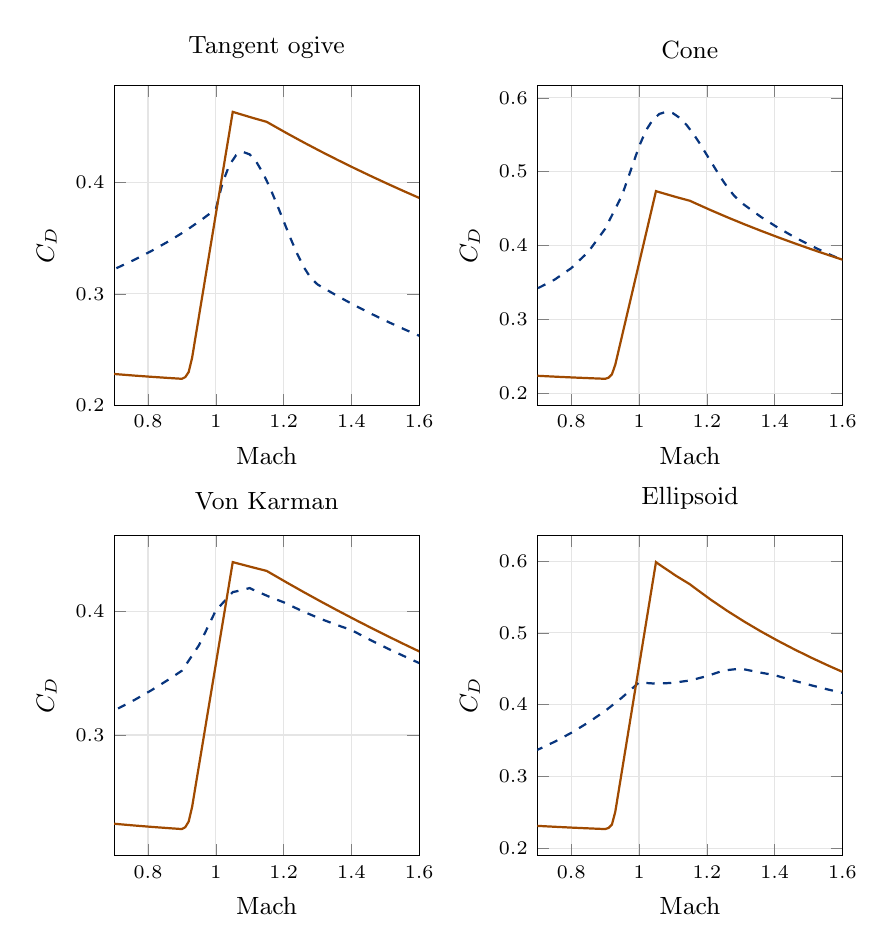
\begin{tikzpicture}
\begin{groupplot}[group style={group size=2 by 2,horizontal sep=1.50cm,vertical sep=1.65cm},width=.45\textwidth,height=5.65cm,grid=major,grid style={gray!20},tick label style={font=\scriptsize},label style={font=\small},title style={font=\small},scaled y ticks=false,yticklabel style={/pgf/number format/fixed,/pgf/number format/precision=3},unbounded coords=jump]
\nextgroupplot[title={Tangent ogive},xlabel={Mach},ylabel={$C_D$},xmin=0.7,xmax=1.6]
\addplot[thick,B,dashed] coordinates {(0.01,0.432385) (0.02,0.3897077) (0.03,0.368739) (0.04,0.355364) (0.05,0.3457716) (0.06,0.3384154) (0.07,0.3325257) (0.08,0.3276676) (0.09,0.3235729) (0.11,0.3170244) (0.13,0.312015) (0.16,0.3064266) (0.18,0.303622) (0.21,0.3004307) (0.26,0.2971293) (0.31,0.2956987) (0.36,0.2957129) (0.41,0.296925) (0.46,0.29918) (0.51,0.3023746) (0.56,0.3064369) (0.61,0.311315) (0.66,0.3169702) (0.71,0.3233731) (0.76,0.3305008) (0.81,0.3383351) (0.86,0.3468615) (0.91,0.3561867) (0.96,0.3667604) (1,0.3758332) (1.01,0.3876035) (1.02,0.3994312) (1.04,0.41525) (1.06,0.4241697) (1.08,0.4270714) (1.1,0.424837) (1.11,0.4213711) (1.12,0.4179431) (1.14,0.4076398) (1.16,0.3948092) (1.18,0.3803337) (1.21,0.3575234) (1.22,0.34998) (1.24,0.3358689) (1.26,0.323647) (1.28,0.3141988) (1.3,0.308409) (1.31,0.3065889) (1.36,0.2978366) (1.41,0.2896227) (1.46,0.2818902) (1.51,0.2745922) (1.56,0.2676872) (1.61,0.2611402) (1.66,0.2549197) (1.71,0.2489988) (1.76,0.2433533) (1.81,0.2379621) (1.86,0.2328059) (1.91,0.2278679) (1.96,0.2231329) (2.01,0.2185872) (2.06,0.2142184) (2.11,0.2100153) (2.16,0.2059678) (2.21,0.2020666) (2.26,0.1983031) (2.31,0.1946698) (2.36,0.1911594) (2.41,0.1877654) (2.46,0.1844817) (2.51,0.1813028) (2.56,0.1782235) (2.61,0.175239) (2.66,0.1723447) (2.71,0.1695367) (2.76,0.1668109) (2.81,0.1641637) (2.86,0.1615918) (2.91,0.1590919) (2.96,0.156661) (3,0.154764)};
\addplot[thick,burntorange] coordinates {(0.01,0.3747526) (0.02,0.3370981) (0.03,0.3184175) (0.04,0.3064439) (0.05,0.2978187) (0.06,0.2911705) (0.07,0.2858134) (0.08,0.2813592) (0.09,0.2775679) (0.11,0.2713925) (0.13,0.2665116) (0.16,0.2607559) (0.18,0.2576371) (0.21,0.2537077) (0.26,0.2485362) (0.31,0.2445031) (0.36,0.2412271) (0.41,0.238487) (0.46,0.2361445) (0.51,0.2341071) (0.56,0.2323107) (0.61,0.2307088) (0.66,0.2292669) (0.71,0.2279585) (0.76,0.2267632) (0.81,0.2256647) (0.86,0.2246499) (0.9,0.2238911) (0.91,0.2254135) (0.92,0.2299809) (0.93,0.2425879) (0.96,0.2976764) (1.01,0.3894907) (1.05,0.4629422) (1.06,0.4619899) (1.11,0.4574285) (1.15,0.4539954) (1.16,0.4522726) (1.21,0.4436996) (1.26,0.4354433) (1.31,0.4274746) (1.36,0.4197684) (1.41,0.412304) (1.46,0.4050635) (1.51,0.3980314) (1.56,0.3911943) (1.61,0.3845406) (1.66,0.3780599) (1.71,0.371743) (1.76,0.3655817) (1.81,0.3595688) (1.86,0.3536978) (1.91,0.3479626) (1.96,0.3423577) (2.01,0.336981) (2.06,0.3321207) (2.11,0.3273803) (2.16,0.3227565) (2.21,0.3182462) (2.26,0.3138469) (2.31,0.3095557) (2.36,0.3053702) (2.41,0.3012879) (2.46,0.2973064) (2.51,0.2934237) (2.56,0.2896372) (2.61,0.2859449) (2.66,0.2823448) (2.71,0.2788348) (2.76,0.2754128) (2.81,0.2720768) (2.86,0.2688251) (2.91,0.2656555) (2.96,0.2625662) (3,0.2601514)};
\nextgroupplot[title={Cone},xlabel={Mach},ylabel={$C_D$},xmin=0.7,xmax=1.6]
\addplot[thick,B,dashed] coordinates {(0.01,0.4410384) (0.02,0.3999209) (0.03,0.3797202) (0.04,0.3668369) (0.05,0.357599) (0.06,0.3505166) (0.07,0.3448482) (0.08,0.3401745) (0.09,0.3362374) (0.11,0.329947) (0.13,0.3251433) (0.16,0.3198003) (0.18,0.3171304) (0.21,0.3141112) (0.26,0.3110424) (0.31,0.3098016) (0.36,0.3099828) (0.41,0.3113592) (0.46,0.3138082) (0.51,0.3172864) (0.56,0.3218352) (0.61,0.3276084) (0.66,0.3349257) (0.7,0.3420819) (0.71,0.3443558) (0.75,0.3537388) (0.76,0.3568391) (0.8,0.3695206) (0.81,0.3738582) (0.85,0.3914841) (0.86,0.3976725) (0.9,0.422697) (0.91,0.4317431) (0.95,0.4682605) (0.96,0.4813555) (1,0.5340751) (1.01,0.5447368) (1.02,0.5554556) (1.04,0.5699144) (1.06,0.5781893) (1.08,0.5810194) (1.1,0.5791442) (1.11,0.5760096) (1.12,0.5729129) (1.14,0.5634201) (1.16,0.5514055) (1.18,0.5376095) (1.21,0.51519) (1.24,0.4929422) (1.26,0.4794319) (1.28,0.4678478) (1.3,0.4589325) (1.31,0.4553664) (1.36,0.4387564) (1.41,0.424201) (1.46,0.4111389) (1.51,0.3993363) (1.56,0.3885158) (1.61,0.3785604) (1.66,0.3693104) (1.71,0.3606981) (1.76,0.3526218) (1.81,0.3450387) (1.86,0.3378791) (1.91,0.3311141) (1.96,0.3246936) (2.01,0.3185969) (2.06,0.3127865) (2.11,0.3072473) (2.16,0.3019502) (2.21,0.2968839) (2.26,0.2920254) (2.31,0.2873657) (2.36,0.2828864) (2.41,0.2785804) (2.46,0.2744327) (2.51,0.2704374) (2.56,0.2665821) (2.61,0.2628619) (2.66,0.2592664) (2.71,0.2557917) (2.76,0.2524287) (2.81,0.2491742) (2.86,0.2460206) (2.91,0.2429649) (2.96,0.2400005) (3,0.237693)};
\addplot[thick,burntorange] coordinates {(0.01,0.3638861) (0.02,0.3278052) (0.03,0.3099244) (0.04,0.2984721) (0.05,0.2902274) (0.06,0.2838757) (0.07,0.2787598) (0.08,0.2745079) (0.09,0.2708901) (0.11,0.265) (0.13,0.2603474) (0.16,0.2548643) (0.18,0.2518948) (0.21,0.2481555) (0.26,0.2432376) (0.31,0.2394053) (0.36,0.2362945) (0.41,0.2336943) (0.46,0.2314726) (0.51,0.2295414) (0.56,0.2278393) (0.61,0.2263223) (0.66,0.2249573) (0.71,0.2237193) (0.76,0.2225887) (0.81,0.22155) (0.86,0.2205908) (0.9,0.2198738) (0.91,0.2213689) (0.92,0.2258544) (0.93,0.2389993) (0.96,0.2976847) (1.01,0.3954936) (1.05,0.4737407) (1.06,0.4723418) (1.11,0.4656795) (1.15,0.4607096) (1.16,0.4586207) (1.21,0.4483168) (1.26,0.4384802) (1.31,0.4290633) (1.36,0.420026) (1.41,0.4113343) (1.46,0.402959) (1.51,0.3948751) (1.56,0.3870607) (1.61,0.379497) (1.66,0.3721671) (1.71,0.3650565) (1.76,0.3581519) (1.81,0.3514417) (1.86,0.3449155) (1.91,0.3385638) (1.96,0.332378) (2.01,0.3264494) (2.06,0.3210532) (2.11,0.3158047) (2.16,0.3106988) (2.21,0.3057305) (2.26,0.3008954) (2.31,0.2961893) (2.36,0.2916083) (2.41,0.2871485) (2.46,0.2828065) (2.51,0.278579) (2.56,0.2744626) (2.61,0.2704544) (2.66,0.2665514) (2.71,0.2627508) (2.76,0.2590498) (2.81,0.2554457) (2.86,0.2519362) (2.91,0.2485185) (2.96,0.2451903) (3,0.2425907)};
\nextgroupplot[title={Von Karman},xlabel={Mach},ylabel={$C_D$},xmin=0.7,xmax=1.6]
\addplot[thick,B,dashed] coordinates {(0.01,0.4294374) (0.02,0.3869424) (0.03,0.3660635) (0.04,0.352746) (0.05,0.3431949) (0.06,0.3358708) (0.07,0.3300069) (0.08,0.3251704) (0.09,0.3210941) (0.1,0.3176028) (0.11,0.3145758) (0.13,0.3095904) (0.14,0.3075196) (0.16,0.3040306) (0.18,0.3012418) (0.21,0.2980706) (0.23,0.2964977) (0.26,0.2947963) (0.28,0.2940383) (0.31,0.2933876) (0.36,0.2934203) (0.41,0.2946486) (0.46,0.2969181) (0.51,0.300126) (0.56,0.3042007) (0.61,0.3090904) (0.66,0.3147567) (0.71,0.3211703) (0.76,0.3283083) (0.81,0.3361527) (0.86,0.3446891) (0.9,0.3520083) (0.91,0.3560236) (0.95,0.3724203) (0.96,0.378004) (1,0.4006815) (1.01,0.4035491) (1.05,0.4155819) (1.06,0.4161249) (1.1,0.4188057) (1.11,0.4175011) (1.16,0.4115277) (1.2,0.4073542) (1.21,0.4059881) (1.26,0.3995847) (1.31,0.393835) (1.36,0.3886687) (1.4,0.3849149) (1.41,0.3834256) (1.46,0.3762536) (1.51,0.3695078) (1.56,0.363149) (1.61,0.356893) (1.66,0.3499598) (1.71,0.3433226) (1.76,0.3369581) (1.81,0.3308454) (1.86,0.3249657) (1.91,0.3193025) (1.96,0.3138406) (2.01,0.3086367) (2.06,0.3038884) (2.11,0.2993047) (2.16,0.2948756) (2.21,0.2905919) (2.26,0.2864452) (2.31,0.2824277) (2.36,0.2785325) (2.41,0.2747531) (2.46,0.2710835) (2.51,0.267518) (2.56,0.2640516) (2.61,0.2606796) (2.66,0.2573974) (2.71,0.2542009) (2.76,0.2510863) (2.81,0.2480499) (2.86,0.2450885) (2.91,0.2421987) (2.96,0.2393776) (3,0.2371683)};
\addplot[thick,burntorange] coordinates {(0.01,0.3747526) (0.02,0.3370981) (0.03,0.3184175) (0.04,0.3064439) (0.05,0.2978187) (0.06,0.2911705) (0.07,0.2858134) (0.08,0.2813592) (0.09,0.2775679) (0.11,0.2713925) (0.13,0.2665116) (0.16,0.2607559) (0.18,0.2576371) (0.21,0.2537077) (0.26,0.2485362) (0.31,0.2445031) (0.36,0.2412271) (0.41,0.238487) (0.46,0.2361445) (0.51,0.2341071) (0.56,0.2323107) (0.61,0.2307088) (0.66,0.2292669) (0.71,0.2279585) (0.76,0.2267632) (0.81,0.2256647) (0.86,0.2246499) (0.9,0.2238911) (0.91,0.2254135) (0.92,0.2299809) (0.93,0.2416627) (0.96,0.2912005) (1.01,0.3737635) (1.05,0.4398139) (1.06,0.4390799) (1.11,0.4354857) (1.15,0.4326966) (1.16,0.4311192) (1.21,0.4231911) (1.26,0.4154615) (1.31,0.4079222) (1.36,0.400565) (1.41,0.3933827) (1.46,0.3863683) (1.51,0.3795156) (1.56,0.3728185) (1.61,0.3662717) (1.66,0.3598698) (1.71,0.3536081) (1.76,0.3474819) (1.81,0.3414869) (1.86,0.3356194) (1.91,0.3298753) (1.96,0.3242509) (2.01,0.3188459) (2.06,0.3139498) (2.11,0.309167) (2.16,0.3044955) (2.21,0.299933) (2.26,0.2954776) (2.31,0.2911272) (2.36,0.2868799) (2.41,0.2827336) (2.46,0.2786864) (2.51,0.2747365) (2.56,0.2708818) (2.61,0.2671206) (2.66,0.2634509) (2.71,0.259871) (2.76,0.2563789) (2.81,0.2529728) (2.86,0.249651) (2.91,0.2464116) (2.96,0.2432528) (3,0.2407826)};
\nextgroupplot[title={Ellipsoid},xlabel={Mach},ylabel={$C_D$},xmin=0.7,xmax=1.6]
\addplot[thick,B,dashed] coordinates {(0.01,0.4385464) (0.02,0.3947994) (0.03,0.373304) (0.04,0.3595919) (0.05,0.3497564) (0.06,0.3422136) (0.07,0.3361734) (0.08,0.3311899) (0.09,0.3269883) (0.1,0.3233882) (0.11,0.3202689) (0.12,0.3175376) (0.13,0.3151284) (0.14,0.3129913) (0.16,0.3093947) (0.18,0.306524) (0.21,0.3032679) (0.23,0.3016692) (0.26,0.2999644) (0.29,0.29898) (0.31,0.2986786) (0.32,0.2986316) (0.36,0.2990205) (0.39,0.2999172) (0.41,0.3007909) (0.44,0.3024932) (0.46,0.3038923) (0.49,0.3063723) (0.51,0.3082877) (0.54,0.3115431) (0.56,0.3139794) (0.59,0.3180254) (0.61,0.3209976) (0.64,0.3258625) (0.66,0.3293932) (0.7,0.3370824) (0.71,0.3392337) (0.75,0.3481279) (0.76,0.3506005) (0.8,0.3607728) (0.81,0.3635869) (0.85,0.3751192) (0.86,0.3782968) (0.9,0.3912789) (0.91,0.3949657) (0.95,0.4100509) (0.96,0.4141874) (1,0.4310783) (1.01,0.430609) (1.05,0.4292967) (1.06,0.4294438) (1.09,0.4301937) (1.11,0.4311101) (1.15,0.4337462) (1.16,0.4348976) (1.2,0.4398283) (1.21,0.441352) (1.25,0.4477344) (1.26,0.4481985) (1.3,0.4503104) (1.31,0.4492995) (1.36,0.4445846) (1.4,0.4411925) (1.41,0.4397936) (1.46,0.4330745) (1.51,0.4267823) (1.56,0.4208779) (1.61,0.4153019) (1.66,0.4099493) (1.71,0.4048935) (1.76,0.400111) (1.81,0.3955809) (1.86,0.3912845) (1.91,0.3872052) (1.96,0.3833279) (2.01,0.3795392) (2.06,0.3755268) (2.11,0.3716797) (2.16,0.3679877) (2.21,0.3644417) (2.26,0.3610333) (2.31,0.3577549) (2.36,0.3545993) (2.41,0.3514851) (2.46,0.3481813) (2.51,0.3449822) (2.56,0.3418829) (2.61,0.3388784) (2.66,0.3359643) (2.71,0.3331366) (2.76,0.3303913) (2.81,0.3277248) (2.86,0.3251337) (2.91,0.3226148) (2.96,0.3201652) (3,0.3182534)};
\addplot[thick,burntorange] coordinates {(0.01,0.3822419) (0.02,0.3435093) (0.03,0.324281) (0.04,0.3119504) (0.05,0.3030647) (0.06,0.2962135) (0.07,0.2906913) (0.08,0.2860986) (0.09,0.2821886) (0.11,0.2758179) (0.13,0.2707808) (0.16,0.2648387) (0.21,0.2575583) (0.26,0.2522135) (0.31,0.2480431) (0.36,0.2446541) (0.41,0.2418185) (0.46,0.2393934) (0.51,0.2372836) (0.56,0.2354227) (0.61,0.2337628) (0.66,0.2322683) (0.71,0.2309119) (0.76,0.2296724) (0.81,0.228533) (0.86,0.2274802) (0.9,0.2266928) (0.91,0.2282343) (0.92,0.2328588) (0.93,0.2508214) (0.96,0.3377865) (1.01,0.4827283) (1.05,0.5986818) (1.06,0.5952638) (1.11,0.5793348) (1.15,0.5678301) (1.16,0.5642155) (1.21,0.5468583) (1.26,0.5308157) (1.31,0.5159109) (1.36,0.5019975) (1.41,0.4889545) (1.46,0.4766805) (1.51,0.4650899) (1.56,0.4541101) (1.61,0.4436796) (1.66,0.4337452) (1.71,0.424261) (1.76,0.4151872) (1.81,0.4064893) (1.86,0.3981371) (1.91,0.3901037) (1.96,0.3823657) (2.01,0.3750074) (2.06,0.3683105) (2.11,0.3618562) (2.16,0.3556302) (2.21,0.3496199) (2.26,0.3438136) (2.31,0.338201) (2.36,0.3327727) (2.41,0.3275196) (2.46,0.322434) (2.51,0.3175086) (2.56,0.3127362) (2.61,0.3081108) (2.66,0.3036263) (2.71,0.2992774) (2.76,0.2950587) (2.81,0.2909654) (2.86,0.2869931) (2.91,0.2831372) (2.96,0.2793937) (3,0.2764772)};
\end{groupplot}\end{tikzpicture}
\caption{Geometry and zero roughness are matched. Different onset, peak Mach and width of the transonic rise remain even in shapes that agree closely at Mach 2.}\label{fig:atlas-29-nose-transonic-detail}
\end{figure}
\noindent{\footnotesize Export files: \code{29-nose-transonic-detail.svg} and \code{29-nose-transonic-detail.png}.\\ Directory: \code{aerodynamic-investigation/extended/figures/}.}

\clearpage\subsubsection*{Body length and fin count controls}
\begin{figure}[H]\centering
{\footnotesize\begin{tabular}{ll}
\tikz[baseline=-.5ex]{\draw[thick,B,dashed] (0,0)--(.40,0);}\ MIT OR & \tikz[baseline=-.5ex]{\draw[thick,burntorange] (0,0)--(.40,0);}\ RASAero\\
\end{tabular}}\par\vspace{.7em}
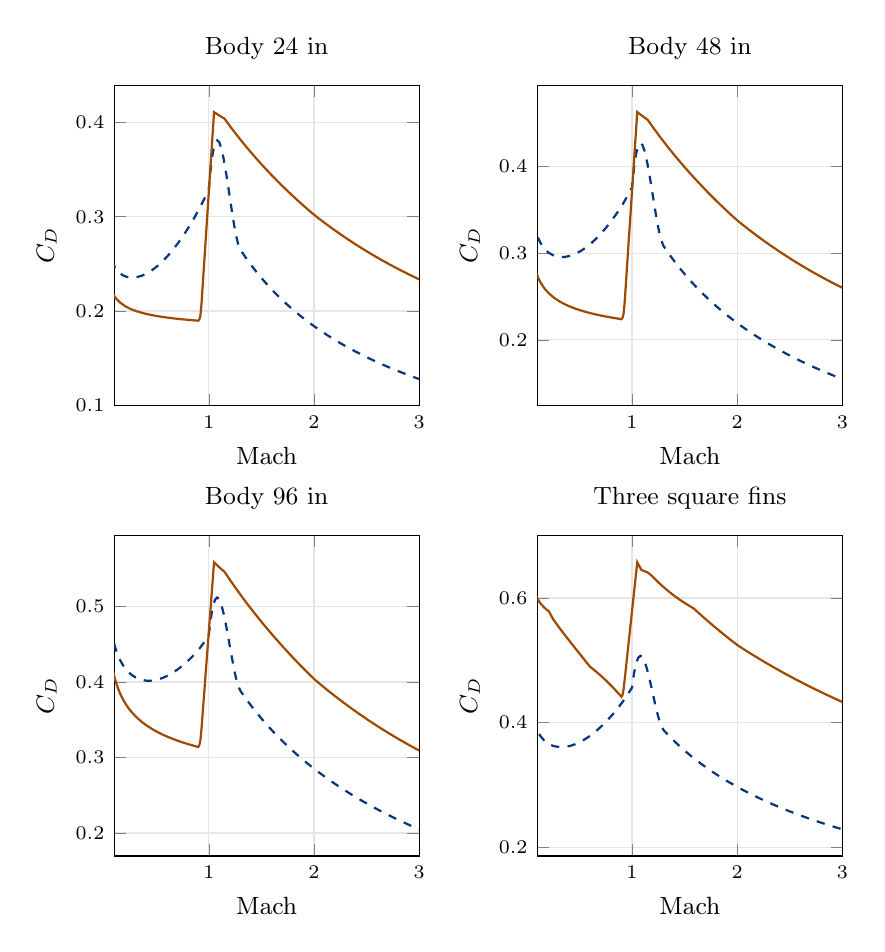
\begin{tikzpicture}
\begin{groupplot}[group style={group size=2 by 2,horizontal sep=1.50cm,vertical sep=1.65cm},width=.45\textwidth,height=5.65cm,grid=major,grid style={gray!20},tick label style={font=\scriptsize},label style={font=\small},title style={font=\small},scaled y ticks=false,yticklabel style={/pgf/number format/fixed,/pgf/number format/precision=3},unbounded coords=jump]
\nextgroupplot[title={Body 24 in},xlabel={Mach},ylabel={$C_D$},xmin=0.1,xmax=3]
\addplot[thick,B,dashed] coordinates {(0.01,0.323665) (0.02,0.2944537) (0.03,0.2802561) (0.04,0.2712667) (0.05,0.2648616) (0.06,0.2599821) (0.07,0.2561029) (0.08,0.2529283) (0.09,0.2502765) (0.11,0.2461012) (0.13,0.2429925) (0.16,0.2396825) (0.18,0.2381342) (0.21,0.2365538) (0.26,0.2354371) (0.31,0.2357825) (0.36,0.2373062) (0.41,0.2398441) (0.46,0.2432935) (0.51,0.2475859) (0.56,0.2526738) (0.61,0.2585228) (0.66,0.2651073) (0.71,0.272408) (0.76,0.2804098) (0.81,0.2891007) (0.86,0.2984711) (0.91,0.3085874) (0.96,0.31973) (1,0.3292047) (1.01,0.3410675) (1.02,0.3529846) (1.04,0.3689717) (1.06,0.3780458) (1.08,0.3810872) (1.1,0.3789774) (1.11,0.3756423) (1.12,0.3723447) (1.14,0.362301) (1.16,0.3497283) (1.18,0.3355089) (1.21,0.3130797) (1.22,0.3056626) (1.24,0.2918029) (1.26,0.2798308) (1.28,0.270631) (1.3,0.265088) (1.31,0.2633908) (1.36,0.2552478) (1.41,0.2476345) (1.46,0.2404941) (1.51,0.23378) (1.56,0.2274509) (1.61,0.2214716) (1.66,0.215811) (1.71,0.2104421) (1.76,0.2053406) (1.81,0.2004855) (1.86,0.1958576) (1.91,0.1914401) (1.96,0.1872177) (2.01,0.1831769) (2.06,0.1793052) (2.11,0.1755914) (2.16,0.1720254) (2.21,0.1685981) (2.26,0.1653008) (2.31,0.162126) (2.36,0.1590665) (2.41,0.1561159) (2.46,0.1532682) (2.51,0.1505178) (2.56,0.1478597) (2.61,0.145289) (2.66,0.1428015) (2.71,0.1403931) (2.76,0.1380598) (2.81,0.1357983) (2.86,0.1336051) (2.91,0.1314772) (2.96,0.1294117) (3,0.1278023)};
\addplot[thick,burntorange] coordinates {(0.01,0.2780421) (0.02,0.2541315) (0.03,0.2425575) (0.04,0.2352641) (0.05,0.2300805) (0.06,0.2261299) (0.07,0.2229777) (0.08,0.2203796) (0.09,0.2181857) (0.11,0.2146495) (0.13,0.2118898) (0.16,0.2086799) (0.21,0.2048221) (0.26,0.2020491) (0.31,0.1999246) (0.36,0.1982259) (0.41,0.1968253) (0.46,0.1956436) (0.51,0.1946283) (0.56,0.1937434) (0.61,0.1929628) (0.66,0.1922673) (0.71,0.1916425) (0.76,0.191077) (0.81,0.190562) (0.86,0.1900904) (0.9,0.1897404) (0.91,0.1910306) (0.92,0.1949013) (0.93,0.2063332) (0.96,0.2575063) (1.01,0.3427947) (1.05,0.4110255) (1.06,0.4102768) (1.11,0.4067172) (1.15,0.4040669) (1.16,0.4025374) (1.21,0.3949169) (1.26,0.3875917) (1.31,0.3805341) (1.36,0.3737209) (1.41,0.3671326) (1.46,0.3607523) (1.51,0.3545658) (1.56,0.3485606) (1.61,0.342726) (1.66,0.3370524) (1.71,0.3315312) (1.76,0.3261551) (1.81,0.3209172) (1.86,0.3158117) (1.91,0.310833) (1.96,0.305976) (2.01,0.3012998) (2.06,0.2969803) (2.11,0.2927719) (2.16,0.2886715) (2.21,0.284676) (2.26,0.2807829) (2.31,0.2769893) (2.36,0.273293) (2.41,0.2696913) (2.46,0.2661821) (2.51,0.2627633) (2.56,0.2594325) (2.61,0.2561877) (2.66,0.253027) (2.71,0.2499485) (2.76,0.2469501) (2.81,0.2440299) (2.86,0.2411862) (2.91,0.2384171) (2.96,0.2357208) (3,0.2336151)};
\nextgroupplot[title={Body 48 in},xlabel={Mach},ylabel={$C_D$},xmin=0.1,xmax=3]
\addplot[thick,B,dashed] coordinates {(0.01,0.432385) (0.02,0.3897077) (0.03,0.368739) (0.04,0.355364) (0.05,0.3457716) (0.06,0.3384154) (0.07,0.3325257) (0.08,0.3276676) (0.09,0.3235729) (0.11,0.3170244) (0.13,0.312015) (0.16,0.3064266) (0.18,0.303622) (0.21,0.3004307) (0.26,0.2971293) (0.31,0.2956987) (0.36,0.2957129) (0.41,0.296925) (0.46,0.29918) (0.51,0.3023746) (0.56,0.3064369) (0.61,0.311315) (0.66,0.3169702) (0.71,0.3233731) (0.76,0.3305008) (0.81,0.3383351) (0.86,0.3468615) (0.91,0.3561867) (0.96,0.3667604) (1,0.3758332) (1.01,0.3876035) (1.02,0.3994312) (1.04,0.41525) (1.06,0.4241697) (1.08,0.4270714) (1.1,0.424837) (1.11,0.4213711) (1.12,0.4179431) (1.14,0.4076398) (1.16,0.3948092) (1.18,0.3803337) (1.21,0.3575234) (1.22,0.34998) (1.24,0.3358689) (1.26,0.323647) (1.28,0.3141988) (1.3,0.308409) (1.31,0.3065889) (1.36,0.2978366) (1.41,0.2896227) (1.46,0.2818902) (1.51,0.2745922) (1.56,0.2676872) (1.61,0.2611402) (1.66,0.2549197) (1.71,0.2489988) (1.76,0.2433533) (1.81,0.2379621) (1.86,0.2328059) (1.91,0.2278679) (1.96,0.2231329) (2.01,0.2185872) (2.06,0.2142184) (2.11,0.2100153) (2.16,0.2059678) (2.21,0.2020666) (2.26,0.1983031) (2.31,0.1946698) (2.36,0.1911594) (2.41,0.1877654) (2.46,0.1844817) (2.51,0.1813028) (2.56,0.1782235) (2.61,0.175239) (2.66,0.1723447) (2.71,0.1695367) (2.76,0.1668109) (2.81,0.1641637) (2.86,0.1615918) (2.91,0.1590919) (2.96,0.156661) (3,0.154764)};
\addplot[thick,burntorange] coordinates {(0.01,0.3747526) (0.02,0.3370981) (0.03,0.3184175) (0.04,0.3064439) (0.05,0.2978187) (0.06,0.2911705) (0.07,0.2858134) (0.08,0.2813592) (0.09,0.2775679) (0.11,0.2713925) (0.13,0.2665116) (0.16,0.2607559) (0.18,0.2576371) (0.21,0.2537077) (0.26,0.2485362) (0.31,0.2445031) (0.36,0.2412271) (0.41,0.238487) (0.46,0.2361445) (0.51,0.2341071) (0.56,0.2323107) (0.61,0.2307088) (0.66,0.2292669) (0.71,0.2279585) (0.76,0.2267632) (0.81,0.2256647) (0.86,0.2246499) (0.9,0.2238911) (0.91,0.2254135) (0.92,0.2299809) (0.93,0.2425879) (0.96,0.2976764) (1.01,0.3894907) (1.05,0.4629422) (1.06,0.4619899) (1.11,0.4574285) (1.15,0.4539954) (1.16,0.4522726) (1.21,0.4436996) (1.26,0.4354433) (1.31,0.4274746) (1.36,0.4197684) (1.41,0.412304) (1.46,0.4050635) (1.51,0.3980314) (1.56,0.3911943) (1.61,0.3845406) (1.66,0.3780599) (1.71,0.371743) (1.76,0.3655817) (1.81,0.3595688) (1.86,0.3536978) (1.91,0.3479626) (1.96,0.3423577) (2.01,0.336981) (2.06,0.3321207) (2.11,0.3273803) (2.16,0.3227565) (2.21,0.3182462) (2.26,0.3138469) (2.31,0.3095557) (2.36,0.3053702) (2.41,0.3012879) (2.46,0.2973064) (2.51,0.2934237) (2.56,0.2896372) (2.61,0.2859449) (2.66,0.2823448) (2.71,0.2788348) (2.76,0.2754128) (2.81,0.2720768) (2.86,0.2688251) (2.91,0.2656555) (2.96,0.2625662) (3,0.2601514)};
\nextgroupplot[title={Body 96 in},xlabel={Mach},ylabel={$C_D$},xmin=0.1,xmax=3]
\addplot[thick,B,dashed] coordinates {(0.01,0.6261331) (0.02,0.5606361) (0.03,0.528105) (0.04,0.5072074) (0.05,0.4921302) (0.06,0.4805018) (0.07,0.471137) (0.08,0.4633639) (0.09,0.4567674) (0.11,0.446096) (0.13,0.4377774) (0.16,0.4282129) (0.18,0.4232115) (0.21,0.4171979) (0.26,0.4100588) (0.31,0.4054988) (0.36,0.4028454) (0.41,0.4017078) (0.46,0.4018404) (0.51,0.4030792) (0.56,0.4053099) (0.61,0.4084499) (0.66,0.4124375) (0.71,0.417226) (0.76,0.4227787) (0.81,0.4290667) (0.86,0.4360668) (0.91,0.4439605) (0.96,0.4535099) (1,0.4618601) (1.01,0.4734642) (1.02,0.4851318) (1.04,0.5006486) (1.06,0.509292) (1.08,0.5119441) (1.1,0.509488) (1.11,0.5057845) (1.12,0.5021197) (1.14,0.4913451) (1.16,0.4780461) (1.18,0.463105) (1.21,0.4396016) (1.24,0.41726) (1.26,0.4045833) (1.28,0.3946829) (1.3,0.3884433) (1.31,0.3863993) (1.36,0.3765365) (1.41,0.3672271) (1.46,0.3584136) (1.51,0.350049) (1.56,0.3420916) (1.61,0.3345062) (1.66,0.3272613) (1.71,0.3203301) (1.76,0.3136882) (1.81,0.3073144) (1.86,0.3011897) (1.91,0.2952972) (1.96,0.2896216) (2.01,0.2841493) (2.06,0.2788679) (2.11,0.2737662) (2.16,0.268834) (2.21,0.2640619) (2.26,0.2594415) (2.31,0.2549651) (2.36,0.2506252) (2.41,0.2464154) (2.46,0.2423296) (2.51,0.2383619) (2.56,0.2345072) (2.61,0.2307605) (2.66,0.2271172) (2.71,0.2235731) (2.76,0.2201239) (2.81,0.2167661) (2.86,0.213496) (2.91,0.2103103) (2.96,0.2072057) (3,0.2047785)};
\addplot[thick,burntorange] coordinates {(0.01,0.5819804) (0.02,0.5182837) (0.03,0.4861721) (0.04,0.4653707) (0.05,0.450265) (0.06,0.4385443) (0.07,0.4290467) (0.08,0.4211106) (0.09,0.414326) (0.1,0.4084223) (0.11,0.4032121) (0.13,0.3943684) (0.14,0.390559) (0.16,0.3838655) (0.18,0.3781378) (0.21,0.3708821) (0.23,0.3667239) (0.26,0.3612603) (0.31,0.3536937) (0.36,0.3475029) (0.41,0.3422919) (0.46,0.3378111) (0.51,0.3338937) (0.56,0.3304228) (0.61,0.3273139) (0.66,0.3245037) (0.71,0.3219438) (0.76,0.3195964) (0.81,0.3174315) (0.86,0.3154248) (0.9,0.3139199) (0.91,0.3160546) (0.92,0.3224586) (0.93,0.3365115) (0.96,0.3920111) (1.01,0.4845104) (1.05,0.5585098) (1.06,0.5571867) (1.11,0.5508004) (1.15,0.5459404) (1.16,0.5438652) (1.21,0.5335547) (1.26,0.5235992) (1.31,0.5139664) (1.36,0.5046287) (1.41,0.495563) (1.46,0.4867491) (1.51,0.4781698) (1.56,0.4698098) (1.61,0.4616561) (1.66,0.4536969) (1.71,0.4459215) (1.76,0.4383209) (1.81,0.4308866) (1.86,0.4236111) (1.91,0.4164875) (1.96,0.4095095) (2.01,0.402847) (2.06,0.3969951) (2.11,0.3912787) (2.16,0.3856946) (2.21,0.3802396) (2.26,0.3749111) (2.31,0.3697063) (2.36,0.3646227) (2.41,0.3596575) (2.46,0.3548084) (2.51,0.3500732) (2.56,0.3454492) (2.61,0.3409343) (2.66,0.3365263) (2.71,0.332223) (2.76,0.328022) (2.81,0.3239213) (2.86,0.3199189) (2.91,0.3160124) (2.96,0.3122) (3,0.3092163)};
\nextgroupplot[title={Three square fins},xlabel={Mach},ylabel={$C_D$},xmin=0.1,xmax=3]
\addplot[thick,B,dashed] coordinates {(0.01,0.5125489) (0.02,0.4649647) (0.03,0.4415871) (0.04,0.4266778) (0.05,0.4159873) (0.06,0.4077914) (0.07,0.4012319) (0.08,0.3958238) (0.09,0.3912681) (0.11,0.3839899) (0.13,0.3784325) (0.16,0.3722525) (0.18,0.3691654) (0.21,0.3656762) (0.23,0.3639616) (0.26,0.3621347) (0.31,0.3607101) (0.36,0.3609281) (0.41,0.3625143) (0.46,0.3652967) (0.51,0.3691613) (0.56,0.374029) (0.61,0.3798433) (0.66,0.3865625) (0.71,0.3941554) (0.76,0.4025981) (0.81,0.4118721) (0.86,0.4219633) (0.91,0.4329926) (0.96,0.4454635) (1,0.456162) (1.01,0.4680713) (1.02,0.4798475) (1.04,0.4955793) (1.06,0.5044312) (1.08,0.5072813) (1.1,0.5050094) (1.11,0.5015066) (1.12,0.4980435) (1.14,0.4876745) (1.16,0.4747831) (1.18,0.4602506) (1.21,0.4373597) (1.22,0.4297904) (1.24,0.4156284) (1.26,0.4033565) (1.28,0.3938587) (1.3,0.3880193) (1.31,0.3861743) (1.36,0.377296) (1.41,0.3689514) (1.46,0.3610821) (1.51,0.3536408) (1.56,0.346586) (1.61,0.3398829) (1.66,0.3335009) (1.71,0.3274134) (1.76,0.3215969) (1.81,0.316031) (1.86,0.3106971) (1.91,0.3055791) (1.96,0.3006621) (2.01,0.2959331) (2.06,0.29138) (2.11,0.2869923) (2.16,0.28276) (2.21,0.2786742) (2.26,0.2747268) (2.31,0.2709103) (2.36,0.2672177) (2.41,0.2636429) (2.46,0.2601797) (2.51,0.256823) (2.56,0.2535676) (2.61,0.2504088) (2.66,0.2473422) (2.71,0.2443639) (2.76,0.2414698) (2.81,0.2386566) (2.86,0.2359207) (2.91,0.2332592) (2.96,0.2306689) (3,0.2286461)};
\addplot[thick,burntorange] coordinates {(0.01,0.6997066) (0.02,0.6620522) (0.03,0.6433716) (0.04,0.631398) (0.05,0.6227728) (0.06,0.6161246) (0.07,0.6107675) (0.08,0.6063132) (0.09,0.602522) (0.11,0.5963465) (0.13,0.5914656) (0.16,0.58571) (0.18,0.5825911) (0.21,0.5786617) (0.25,0.5661751) (0.26,0.5637556) (0.31,0.5521169) (0.36,0.5410002) (0.41,0.5301839) (0.46,0.51953) (0.51,0.508946) (0.56,0.4983676) (0.6,0.4898774) (0.61,0.4885974) (0.66,0.4817472) (0.71,0.4743851) (0.76,0.4664902) (0.81,0.4580463) (0.86,0.4490404) (0.9,0.4414237) (0.91,0.4444254) (0.92,0.4534304) (0.93,0.4680652) (0.96,0.5153508) (1.01,0.5941602) (1.05,0.6572077) (1.06,0.654136) (1.09,0.6450908) (1.11,0.6436945) (1.15,0.6411508) (1.16,0.6397108) (1.19,0.6353657) (1.21,0.6318905) (1.26,0.6236808) (1.31,0.616093) (1.36,0.6090713) (1.41,0.6025736) (1.46,0.5965666) (1.51,0.5910235) (1.56,0.5859227) (1.59,0.5827963) (1.61,0.5796669) (1.66,0.5720094) (1.71,0.5645655) (1.76,0.557311) (1.81,0.5502259) (1.86,0.543294) (1.91,0.5365013) (1.96,0.5298364) (2.01,0.5234908) (2.06,0.5180314) (2.11,0.5126849) (2.16,0.5074468) (2.21,0.5023132) (2.26,0.497281) (2.31,0.4923472) (2.36,0.4875095) (2.41,0.482765) (2.46,0.4781118) (2.51,0.4735477) (2.56,0.4690703) (2.61,0.4646776) (2.66,0.4603674) (2.71,0.4561375) (2.76,0.4519857) (2.81,0.4479094) (2.86,0.4439064) (2.91,0.4399741) (2.96,0.4361099) (3,0.4330659)};
\end{groupplot}\end{tikzpicture}
\caption{The first three panels vary only finless-body length. The fourth checks the 3-fin count against the original 4-fin family.}\label{fig:atlas-07-body-length}
\end{figure}
\noindent{\footnotesize Export files: \code{07-body-length.svg} and \code{07-body-length.png}.\\ Directory: \code{aerodynamic-investigation/extended/figures/}.}

\clearpage\subsubsection*{Square fin thickness sweep}
\begin{figure}[H]\centering
{\footnotesize\begin{tabular}{ll}
\tikz[baseline=-.5ex]{\draw[thick,B,dashed] (0,0)--(.40,0);}\ MIT OR & \tikz[baseline=-.5ex]{\draw[thick,burntorange] (0,0)--(.40,0);}\ RASAero\\
\end{tabular}}\par\vspace{.7em}
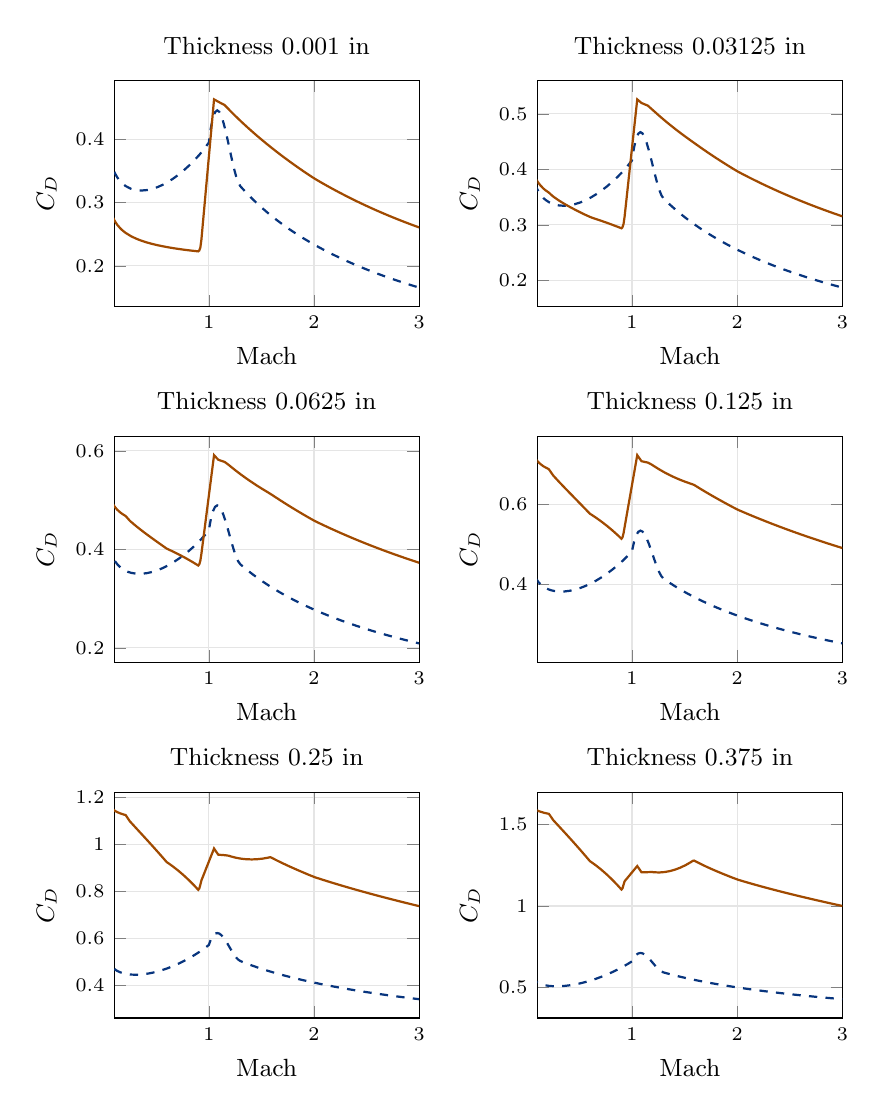
\begin{tikzpicture}
\begin{groupplot}[group style={group size=2 by 3,horizontal sep=1.50cm,vertical sep=1.65cm},width=.45\textwidth,height=4.45cm,grid=major,grid style={gray!20},tick label style={font=\scriptsize},label style={font=\small},title style={font=\small},scaled y ticks=false,yticklabel style={/pgf/number format/fixed,/pgf/number format/precision=3},unbounded coords=jump]
\nextgroupplot[title={Thickness 0.001 in},xlabel={Mach},ylabel={$C_D$},xmin=0.1,xmax=3]
\addplot[thick,B,dashed] coordinates {(0.01,0.4779451) (0.02,0.4290703) (0.03,0.4050499) (0.04,0.3897213) (0.05,0.3787203) (0.06,0.3702764) (0.07,0.3635079) (0.08,0.357917) (0.09,0.3531965) (0.11,0.3456234) (0.13,0.3397977) (0.16,0.3332363) (0.18,0.3298981) (0.21,0.3260256) (0.26,0.3218072) (0.31,0.3196378) (0.36,0.3190297) (0.41,0.3197002) (0.46,0.3214717) (0.51,0.324226) (0.56,0.3278808) (0.61,0.3323765) (0.66,0.3376691) (0.71,0.3437247) (0.76,0.3505172) (0.81,0.3580258) (0.86,0.3662339) (0.91,0.3752637) (0.96,0.3856301) (1,0.3945593) (1.01,0.4062939) (1.02,0.4180853) (1.04,0.4338353) (1.06,0.442692) (1.08,0.4455365) (1.1,0.443251) (1.11,0.4397331) (1.12,0.4362533) (1.14,0.4258472) (1.16,0.4129145) (1.18,0.3983376) (1.21,0.3753767) (1.22,0.3677834) (1.24,0.3535731) (1.26,0.3412527) (1.28,0.3317065) (1.3,0.3258195) (1.31,0.3239509) (1.36,0.3149589) (1.41,0.3065089) (1.46,0.2985438) (1.51,0.2910166) (1.56,0.2838857) (1.61,0.2771161) (1.66,0.2706763) (1.71,0.2645393) (1.76,0.2586809) (1.81,0.2530799) (1.86,0.2477171) (1.91,0.2425757) (1.96,0.2376404) (2.01,0.2328976) (2.06,0.2283347) (2.11,0.2239408) (2.16,0.2197054) (2.21,0.2156194) (2.26,0.2116743) (2.31,0.2078623) (2.36,0.2041762) (2.41,0.2006096) (2.46,0.1971562) (2.51,0.1938105) (2.56,0.1905674) (2.61,0.1874219) (2.66,0.1843696) (2.71,0.1814062) (2.76,0.1785278) (2.81,0.1757309) (2.86,0.1730118) (2.91,0.1703675) (2.96,0.1677947) (3,0.1657862)};
\addplot[thick,burntorange] coordinates {(0.01,0.3731641) (0.02,0.3355096) (0.03,0.3168291) (0.04,0.3048554) (0.05,0.2962303) (0.06,0.289582) (0.07,0.2842249) (0.08,0.2797707) (0.09,0.2759794) (0.11,0.269804) (0.13,0.2649231) (0.16,0.2591674) (0.18,0.2560486) (0.21,0.2521192) (0.26,0.2470096) (0.31,0.243025) (0.36,0.2397988) (0.41,0.2371101) (0.46,0.2348205) (0.51,0.2328375) (0.56,0.231097) (0.61,0.229547) (0.66,0.2281395) (0.71,0.2268697) (0.76,0.225717) (0.81,0.2246652) (0.86,0.2237012) (0.9,0.222986) (0.91,0.2245023) (0.92,0.2290512) (0.93,0.2416782) (0.96,0.2969697) (1.01,0.3891222) (1.05,0.4628442) (1.06,0.4619137) (1.11,0.4574325) (1.15,0.454029) (1.16,0.4523137) (1.21,0.4437686) (1.26,0.4355297) (1.31,0.4275792) (1.36,0.4198921) (1.41,0.4124473) (1.46,0.4052268) (1.51,0.3982149) (1.56,0.3913981) (1.61,0.3847647) (1.66,0.378304) (1.71,0.372007) (1.76,0.3658654) (1.81,0.3598719) (1.86,0.35402) (1.91,0.3483036) (1.96,0.3427171) (2.01,0.3373579) (2.06,0.3325123) (2.11,0.3277862) (2.16,0.3231763) (2.21,0.3186795) (2.26,0.3142932) (2.31,0.3100148) (2.36,0.3058416) (2.41,0.3017712) (2.46,0.2978013) (2.51,0.2939297) (2.56,0.2901539) (2.61,0.2864721) (2.66,0.282882) (2.71,0.2793816) (2.76,0.2759689) (2.81,0.2726418) (2.86,0.2693986) (2.91,0.2662371) (2.96,0.2631555) (3,0.2607466)};
\nextgroupplot[title={Thickness 0.03125 in},xlabel={Mach},ylabel={$C_D$},xmin=0.1,xmax=3]
\addplot[thick,B,dashed] coordinates {(0.01,0.4929054) (0.02,0.4439464) (0.03,0.419887) (0.04,0.404536) (0.05,0.3935214) (0.06,0.3850697) (0.07,0.3782978) (0.08,0.3727067) (0.09,0.3679889) (0.11,0.3604284) (0.13,0.3546236) (0.16,0.3481071) (0.18,0.3448072) (0.21,0.3410041) (0.26,0.3369312) (0.31,0.334944) (0.36,0.334554) (0.41,0.3354783) (0.46,0.3375393) (0.51,0.3406189) (0.56,0.3446351) (0.61,0.3495287) (0.66,0.3552558) (0.71,0.3617832) (0.76,0.3690852) (0.81,0.3771416) (0.86,0.3859363) (0.91,0.3955924) (0.96,0.4066265) (1,0.4161195) (1.01,0.427908) (1.02,0.4396915) (1.04,0.45543) (1.06,0.46428) (1.08,0.4671217) (1.1,0.4648365) (1.11,0.4613192) (1.12,0.4578407) (1.14,0.4474383) (1.16,0.4345107) (1.18,0.41994) (1.21,0.3969896) (1.22,0.3894001) (1.24,0.3751974) (1.26,0.3628848) (1.28,0.3533464) (1.3,0.3474669) (1.31,0.3456021) (1.36,0.3366276) (1.41,0.3281926) (1.46,0.3202398) (1.51,0.3127219) (1.56,0.3055974) (1.61,0.2988313) (1.66,0.2923925) (1.71,0.286254) (1.76,0.2803919) (1.81,0.2747853) (1.86,0.2694151) (1.91,0.2642648) (1.96,0.2593191) (2.01,0.2545647) (2.06,0.2499893) (2.11,0.2455818) (2.16,0.2413322) (2.21,0.2372313) (2.26,0.2332706) (2.31,0.2294426) (2.36,0.2257401) (2.41,0.2221568) (2.46,0.2186864) (2.51,0.2153236) (2.56,0.2120632) (2.61,0.2089003) (2.66,0.2058304) (2.71,0.2028496) (2.76,0.1999537) (2.81,0.1971393) (2.86,0.1944028) (2.91,0.1917411) (2.96,0.1891511) (3,0.1871288)};
\addplot[thick,burntorange] coordinates {(0.01,0.479249) (0.02,0.4415945) (0.03,0.422914) (0.04,0.4109404) (0.05,0.4023152) (0.06,0.3956669) (0.07,0.3903099) (0.08,0.3858556) (0.09,0.3820643) (0.11,0.3758889) (0.13,0.371008) (0.16,0.3652524) (0.18,0.3621335) (0.21,0.3582041) (0.24,0.352975) (0.26,0.3499131) (0.31,0.3434427) (0.36,0.337654) (0.41,0.3323259) (0.46,0.3273199) (0.51,0.3225437) (0.56,0.3179331) (0.61,0.3137135) (0.66,0.3105385) (0.71,0.3072902) (0.76,0.3039479) (0.81,0.3004956) (0.86,0.2969199) (0.9,0.2939634) (0.91,0.2959623) (0.92,0.3019592) (0.93,0.3152408) (0.96,0.3679448) (1.01,0.4557847) (1.05,0.5260566) (1.06,0.5244315) (1.09,0.5196663) (1.11,0.518018) (1.15,0.5148793) (1.16,0.5132363) (1.21,0.5047871) (1.26,0.4963477) (1.31,0.488245) (1.36,0.4804469) (1.41,0.4729265) (1.46,0.4656611) (1.51,0.4586307) (1.56,0.4518186) (1.61,0.4450783) (1.66,0.4383779) (1.71,0.4318417) (1.76,0.4254589) (1.81,0.4192199) (1.86,0.4131169) (1.91,0.4071423) (1.96,0.4012899) (2.01,0.3956883) (2.06,0.3907158) (2.11,0.3858556) (2.16,0.3811047) (2.21,0.3764602) (2.26,0.3719197) (2.31,0.3674806) (2.36,0.3631409) (2.41,0.3588982) (2.46,0.3547505) (2.51,0.3506958) (2.56,0.346732) (2.61,0.3428571) (2.66,0.3390691) (2.71,0.3353662) (2.76,0.3317462) (2.81,0.3282072) (2.86,0.3247473) (2.91,0.3213642) (2.96,0.318056) (3,0.3154621)};
\nextgroupplot[title={Thickness 0.0625 in},xlabel={Mach},ylabel={$C_D$},xmin=0.1,xmax=3]
\addplot[thick,B,dashed] coordinates {(0.01,0.5083604) (0.02,0.4593144) (0.03,0.4352146) (0.04,0.4198403) (0.05,0.4088118) (0.06,0.400352) (0.07,0.3935765) (0.08,0.3879853) (0.09,0.3832703) (0.11,0.3757228) (0.13,0.3699396) (0.16,0.3634696) (0.18,0.3602092) (0.21,0.3564776) (0.23,0.3546085) (0.26,0.3525552) (0.31,0.3507562) (0.36,0.3505915) (0.41,0.351778) (0.46,0.3541381) (0.51,0.3575538) (0.56,0.3619433) (0.61,0.3672478) (0.66,0.3734238) (0.71,0.3804386) (0.76,0.388267) (0.81,0.3968892) (0.86,0.4062899) (0.91,0.4165931) (0.96,0.428317) (1,0.4383924) (1.01,0.4502367) (1.02,0.462012) (1.04,0.4777386) (1.06,0.4865817) (1.08,0.4894204) (1.1,0.4871355) (1.11,0.483619) (1.12,0.4801416) (1.14,0.4697431) (1.16,0.4568208) (1.18,0.4422565) (1.21,0.419317) (1.22,0.4117313) (1.24,0.3975366) (1.26,0.385232) (1.28,0.3757016) (1.3,0.3698299) (1.31,0.367969) (1.36,0.3590126) (1.41,0.3505932) (1.46,0.342653) (1.51,0.3351447) (1.56,0.3280268) (1.61,0.3212644) (1.66,0.3148265) (1.71,0.3086865) (1.76,0.3028207) (1.81,0.2972082) (1.86,0.2918304) (1.91,0.2866708) (1.96,0.2817145) (2.01,0.2769482) (2.06,0.2723597) (2.11,0.2679383) (2.16,0.2636739) (2.21,0.2595575) (2.26,0.2555808) (2.31,0.2517363) (2.36,0.2480169) (2.41,0.2444163) (2.46,0.2409284) (2.51,0.2375479) (2.56,0.2342695) (2.61,0.2310886) (2.66,0.2280008) (2.71,0.2250018) (2.76,0.2220879) (2.81,0.2192554) (2.86,0.2165009) (2.91,0.2138213) (2.96,0.2112135) (3,0.209177)};
\addplot[thick,burntorange] coordinates {(0.01,0.5888409) (0.02,0.5511864) (0.03,0.5325059) (0.04,0.5205322) (0.05,0.5119071) (0.06,0.5052588) (0.07,0.4999018) (0.08,0.4954475) (0.09,0.4916562) (0.11,0.4854808) (0.13,0.4805999) (0.16,0.4748443) (0.18,0.4717254) (0.21,0.467796) (0.25,0.4581274) (0.26,0.4562183) (0.31,0.4471801) (0.36,0.4387442) (0.41,0.4306893) (0.46,0.4228772) (0.51,0.4152155) (0.56,0.4076398) (0.6,0.4016096) (0.61,0.4006624) (0.66,0.3956615) (0.71,0.3903692) (0.76,0.384765) (0.81,0.3788327) (0.86,0.372559) (0.9,0.3672871) (0.91,0.3697847) (0.92,0.3772773) (0.93,0.3912353) (0.96,0.4412661) (1.01,0.5246509) (1.05,0.5913587) (1.06,0.5890159) (1.09,0.5821273) (1.11,0.5806064) (1.15,0.577753) (1.16,0.5761967) (1.19,0.5714753) (1.21,0.5679429) (1.26,0.5594397) (1.31,0.5513638) (1.36,0.5436739) (1.41,0.5363366) (1.46,0.5293238) (1.51,0.5226118) (1.56,0.5161806) (1.61,0.5094868) (1.66,0.5024384) (1.71,0.4955655) (1.76,0.4888527) (1.81,0.482287) (1.86,0.4758577) (1.91,0.4695552) (1.96,0.4633715) (2.01,0.4574673) (2.06,0.4523152) (2.11,0.4472714) (2.16,0.4423328) (2.21,0.4374961) (2.26,0.4327591) (2.31,0.4281192) (2.36,0.4235745) (2.41,0.4191226) (2.46,0.4147618) (2.51,0.41049) (2.56,0.4063052) (2.61,0.4022056) (2.66,0.3981892) (2.71,0.394254) (2.76,0.390398) (2.81,0.386619) (2.86,0.382915) (2.91,0.3792837) (2.96,0.375723) (3,0.3729236)};
\nextgroupplot[title={Thickness 0.125 in},xlabel={Mach},ylabel={$C_D$},xmin=0.1,xmax=3]
\addplot[thick,B,dashed] coordinates {(0.01,0.5392703) (0.02,0.4900503) (0.03,0.4658697) (0.04,0.450449) (0.05,0.4393925) (0.06,0.4309168) (0.07,0.424134) (0.08,0.4185425) (0.09,0.4138331) (0.11,0.4063117) (0.13,0.4005716) (0.16,0.3941944) (0.18,0.3910132) (0.21,0.3874247) (0.23,0.3856667) (0.26,0.3838032) (0.31,0.3823806) (0.36,0.3826665) (0.41,0.3843774) (0.46,0.3873356) (0.51,0.3914235) (0.56,0.3965597) (0.61,0.4026861) (0.66,0.40976) (0.71,0.4177495) (0.76,0.4266305) (0.81,0.4363845) (0.86,0.4469972) (0.91,0.4585945) (0.96,0.4716979) (1,0.4829383) (1.01,0.4948939) (1.02,0.5066529) (1.04,0.5223558) (1.06,0.531185) (1.08,0.5340179) (1.1,0.5317335) (1.11,0.5282184) (1.12,0.5247436) (1.14,0.5143528) (1.16,0.5014411) (1.18,0.4868895) (1.21,0.4639718) (1.22,0.4563939) (1.24,0.442215) (1.26,0.4299264) (1.28,0.420412) (1.3,0.4145561) (1.31,0.4127028) (1.36,0.4037825) (1.41,0.3953943) (1.46,0.3874794) (1.51,0.3799903) (1.56,0.3728856) (1.61,0.3661305) (1.66,0.3596946) (1.71,0.3535516) (1.76,0.3476781) (1.81,0.342054) (1.86,0.3366609) (1.91,0.3314828) (1.96,0.3265051) (2.01,0.321715) (2.06,0.3171006) (2.11,0.3126512) (2.16,0.3083573) (2.21,0.3042101) (2.26,0.3002013) (2.31,0.2963238) (2.36,0.2925705) (2.41,0.2889353) (2.46,0.2854124) (2.51,0.2819964) (2.56,0.2786823) (2.61,0.2754654) (2.66,0.2723414) (2.71,0.2693063) (2.76,0.2663562) (2.81,0.2634875) (2.86,0.2606971) (2.91,0.2579816) (2.96,0.2553382) (3,0.2532734)};
\addplot[thick,burntorange] coordinates {(0.01,0.8080247) (0.02,0.7703703) (0.03,0.7516897) (0.04,0.7397161) (0.05,0.7310909) (0.06,0.7244427) (0.07,0.7190856) (0.08,0.7146313) (0.09,0.71084) (0.11,0.7046646) (0.13,0.6997837) (0.16,0.6940281) (0.21,0.6869798) (0.25,0.6717458) (0.26,0.6688288) (0.31,0.6546548) (0.36,0.6409243) (0.41,0.6274162) (0.46,0.6139917) (0.51,0.6005588) (0.56,0.5870533) (0.6,0.5761646) (0.61,0.5745601) (0.66,0.5659074) (0.71,0.5565273) (0.76,0.5463991) (0.81,0.5355068) (0.86,0.5238373) (0.9,0.5139346) (0.91,0.5174294) (0.92,0.5279136) (0.96,0.5879089) (1.01,0.6623833) (1.05,0.7219628) (1.06,0.7181847) (1.09,0.7070495) (1.11,0.7057831) (1.15,0.7035359) (1.16,0.7021903) (1.19,0.6981246) (1.21,0.6946208) (1.26,0.6864266) (1.31,0.6789658) (1.36,0.6721722) (1.41,0.6659967) (1.46,0.660401) (1.51,0.6553543) (1.56,0.6508322) (1.59,0.6480014) (1.61,0.644709) (1.66,0.6366592) (1.71,0.6288397) (1.76,0.6212208) (1.81,0.6137783) (1.86,0.6064927) (1.91,0.5993475) (1.96,0.5923293) (2.01,0.5856607) (2.06,0.5800016) (2.11,0.5744531) (2.16,0.5690102) (2.21,0.5636688) (2.26,0.5584257) (2.31,0.5532778) (2.36,0.5482225) (2.41,0.5432574) (2.46,0.5383803) (2.51,0.533589) (2.56,0.5288813) (2.61,0.5242552) (2.66,0.5197083) (2.71,0.5152385) (2.76,0.5108433) (2.81,0.5065202) (2.86,0.5022668) (2.91,0.4980803) (2.96,0.4939578) (3,0.4907041)};
\nextgroupplot[title={Thickness 0.25 in},xlabel={Mach},ylabel={$C_D$},xmin=0.1,xmax=3]
\addplot[thick,B,dashed] coordinates {(0.01,0.60109) (0.02,0.5515222) (0.03,0.5271801) (0.04,0.5116665) (0.05,0.5005539) (0.06,0.4920462) (0.07,0.485249) (0.08,0.479657) (0.09,0.4749588) (0.11,0.4674894) (0.13,0.4618357) (0.16,0.4556442) (0.18,0.4526212) (0.21,0.449319) (0.23,0.4477832) (0.26,0.4462991) (0.31,0.4456293) (0.36,0.4468165) (0.41,0.4495762) (0.46,0.4537307) (0.51,0.4591629) (0.56,0.4657925) (0.61,0.4735626) (0.66,0.4824322) (0.71,0.4923713) (0.76,0.5033576) (0.81,0.5153751) (0.86,0.5284118) (0.91,0.5425974) (0.96,0.5584598) (1,0.5720301) (1.01,0.5842085) (1.02,0.5959348) (1.04,0.6115901) (1.06,0.6203916) (1.08,0.6232129) (1.1,0.6209296) (1.11,0.6174173) (1.12,0.6139475) (1.14,0.6035721) (1.16,0.5906817) (1.18,0.5761556) (1.21,0.5532814) (1.22,0.5457189) (1.24,0.5315716) (1.26,0.5193152) (1.28,0.5098328) (1.3,0.5040083) (1.31,0.5021704) (1.36,0.4933224) (1.41,0.4849965) (1.46,0.4771323) (1.51,0.4696816) (1.56,0.4626031) (1.61,0.4558628) (1.66,0.4494308) (1.71,0.4432817) (1.76,0.4373931) (1.81,0.4317456) (1.86,0.426322) (1.91,0.4211069) (1.96,0.4160865) (2.01,0.4112487) (2.06,0.4065822) (2.11,0.4020771) (2.16,0.3977242) (2.21,0.3935152) (2.26,0.3894423) (2.31,0.3854986) (2.36,0.3816777) (2.41,0.3779734) (2.46,0.3743804) (2.51,0.3708935) (2.56,0.3675078) (2.61,0.3642189) (2.66,0.3610227) (2.71,0.3579152) (2.76,0.3548927) (2.81,0.3519519) (2.86,0.3490895) (2.91,0.3463023) (2.96,0.3435876) (3,0.3414661)};
\addplot[thick,burntorange] coordinates {(0.01,1.246392) (0.02,1.208738) (0.03,1.190057) (0.04,1.178083) (0.05,1.169458) (0.06,1.16281) (0.08,1.152999) (0.11,1.143032) (0.13,1.138151) (0.16,1.132395) (0.21,1.125347) (0.25,1.098983) (0.26,1.09405) (0.31,1.069604) (0.36,1.045285) (0.41,1.02087) (0.46,0.9962209) (0.51,0.9712458) (0.56,0.9458799) (0.6,0.9252748) (0.61,0.9223557) (0.66,0.9063993) (0.71,0.8888434) (0.76,0.8696674) (0.81,0.8488553) (0.86,0.8263936) (0.9,0.8072296) (0.91,0.8127188) (0.92,0.8291863) (0.93,0.8472023) (0.96,0.8811945) (1.01,0.9378482) (1.05,0.9831711) (1.06,0.9765224) (1.09,0.9568937) (1.11,0.9561366) (1.16,0.954468) (1.19,0.9523421) (1.21,0.9494415) (1.26,0.9436123) (1.31,0.9396276) (1.36,0.9373455) (1.41,0.9366771) (1.46,0.9375624) (1.51,0.9399606) (1.56,0.9438453) (1.58,0.9458117) (1.59,0.9454377) (1.61,0.9407746) (1.66,0.9294998) (1.71,0.9186941) (1.76,0.9082784) (1.81,0.8981891) (1.86,0.8883762) (1.91,0.8787984) (1.96,0.8694227) (2.01,0.8605887) (2.06,0.8533247) (2.11,0.8462161) (2.16,0.8392505) (2.21,0.8324178) (2.26,0.82571) (2.31,0.8191199) (2.36,0.8126418) (2.41,0.8062702) (2.46,0.8000009) (2.51,0.7938294) (2.56,0.7877517) (2.61,0.7817639) (2.66,0.7758621) (2.71,0.7700424) (2.76,0.7643009) (2.81,0.7586334) (2.86,0.7530356) (2.91,0.7475032) (2.96,0.7420316) (3,0.7376948)};
\nextgroupplot[title={Thickness 0.375 in},xlabel={Mach},ylabel={$C_D$},xmin=0.1,xmax=3]
\addplot[thick,B,dashed] coordinates {(0.01,0.6629098) (0.02,0.6129941) (0.03,0.5884904) (0.04,0.5728839) (0.05,0.5617154) (0.06,0.5531756) (0.07,0.5463639) (0.08,0.5407714) (0.09,0.5360844) (0.11,0.5286671) (0.13,0.5230997) (0.16,0.5170939) (0.18,0.5142293) (0.21,0.5112132) (0.23,0.5098997) (0.26,0.508795) (0.31,0.508878) (0.36,0.5109665) (0.41,0.514775) (0.46,0.5201258) (0.51,0.5269023) (0.56,0.5350253) (0.61,0.5444392) (0.66,0.5551045) (0.71,0.566993) (0.76,0.5800848) (0.81,0.5943657) (0.86,0.6098264) (0.91,0.6266002) (0.96,0.6452217) (1,0.6611219) (1.01,0.6735231) (1.02,0.6852167) (1.04,0.7008245) (1.06,0.7095983) (1.08,0.7124079) (1.1,0.7101256) (1.11,0.7066162) (1.12,0.7031514) (1.14,0.6927914) (1.16,0.6799222) (1.18,0.6654216) (1.21,0.642591) (1.22,0.6350439) (1.24,0.6209283) (1.26,0.6087039) (1.28,0.5992535) (1.3,0.5934605) (1.31,0.591638) (1.36,0.5828623) (1.41,0.5745987) (1.46,0.5667851) (1.51,0.5593729) (1.56,0.5523207) (1.61,0.5455951) (1.66,0.5391669) (1.71,0.5330117) (1.76,0.527108) (1.81,0.5214373) (1.86,0.5159831) (1.91,0.5107309) (1.96,0.5056679) (2.01,0.5007824) (2.06,0.4960639) (2.11,0.491503) (2.16,0.4870911) (2.21,0.4828202) (2.26,0.4786832) (2.31,0.4746735) (2.36,0.4707848) (2.41,0.4670115) (2.46,0.4633484) (2.51,0.4597905) (2.56,0.4563333) (2.61,0.4529725) (2.66,0.449704) (2.71,0.4465241) (2.76,0.4434293) (2.81,0.4404163) (2.86,0.4374819) (2.91,0.434623) (2.96,0.431837) (3,0.4296589)};
\addplot[thick,burntorange] coordinates {(0.01,1.68476) (0.02,1.647105) (0.03,1.628425) (0.04,1.616451) (0.05,1.607826) (0.06,1.601178) (0.08,1.591366) (0.11,1.5814) (0.16,1.570763) (0.21,1.563715) (0.22,1.555051) (0.25,1.52622) (0.26,1.519271) (0.31,1.484554) (0.36,1.449645) (0.41,1.414324) (0.46,1.37845) (0.51,1.341933) (0.56,1.304707) (0.6,1.274385) (0.61,1.270151) (0.66,1.246891) (0.71,1.22116) (0.76,1.192936) (0.81,1.162204) (0.86,1.12895) (0.9,1.100525) (0.91,1.108008) (0.92,1.130459) (0.93,1.15118) (0.96,1.17448) (1.01,1.213313) (1.05,1.244379) (1.06,1.23486) (1.09,1.206738) (1.11,1.20649) (1.16,1.207133) (1.19,1.207785) (1.21,1.206216) (1.26,1.20508) (1.31,1.207566) (1.36,1.213421) (1.41,1.222504) (1.46,1.234733) (1.51,1.250062) (1.56,1.268472) (1.58,1.276697) (1.59,1.277744) (1.61,1.271002) (1.66,1.254872) (1.71,1.239623) (1.76,1.225098) (1.81,1.211171) (1.86,1.197744) (1.91,1.184738) (1.96,1.172087) (2.01,1.160238) (2.06,1.150581) (2.11,1.141179) (2.16,1.132005) (2.21,1.123038) (2.26,1.114262) (2.31,1.105662) (2.36,1.097225) (2.41,1.088941) (2.46,1.0808) (2.51,1.072793) (2.56,1.064913) (2.61,1.057152) (2.66,1.049503) (2.71,1.04196) (2.76,1.034515) (2.81,1.027161) (2.86,1.019891) (2.91,1.012699) (2.96,1.005577) (3,0.9999252)};
\end{groupplot}\end{tikzpicture}
\caption{Fixed planform and sweep. The 0.001 in case is an asymptotic diagnostic, not a representative hardware design.}\label{fig:atlas-08-Hsq-thickness}
\end{figure}
\noindent{\footnotesize Export files: \code{08-Hsq-thickness.svg} and \code{08-Hsq-thickness.png}.\\ Directory: \code{aerodynamic-investigation/extended/figures/}.}

\clearpage\subsubsection*{Beveled fin thickness sweep}
\begin{figure}[H]\centering
{\footnotesize\begin{tabular}{ll}
\tikz[baseline=-.5ex]{\draw[thick,B,dashed] (0,0)--(.40,0);}\ MIT OR & \tikz[baseline=-.5ex]{\draw[thick,burntorange] (0,0)--(.40,0);}\ RASAero\\
\end{tabular}}\par\vspace{.7em}
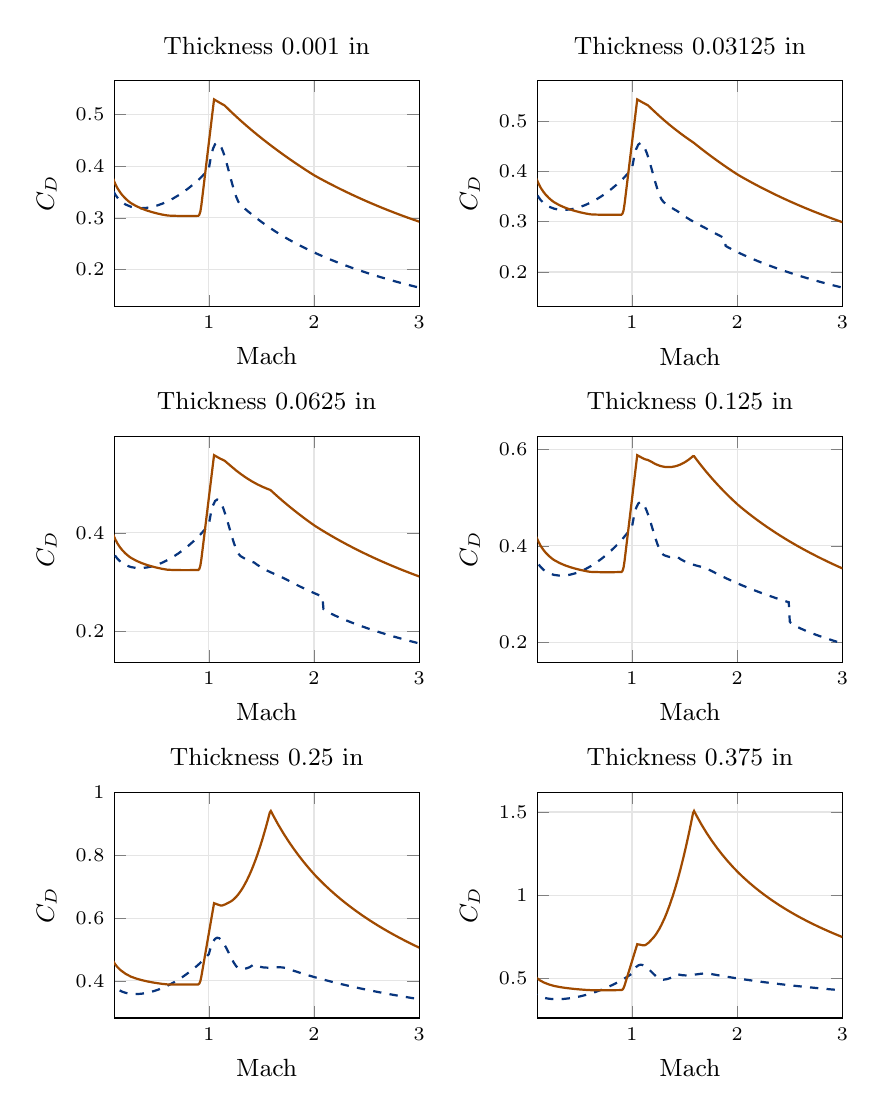
\begin{tikzpicture}
\begin{groupplot}[group style={group size=2 by 3,horizontal sep=1.50cm,vertical sep=1.65cm},width=.45\textwidth,height=4.45cm,grid=major,grid style={gray!20},tick label style={font=\scriptsize},label style={font=\small},title style={font=\small},scaled y ticks=false,yticklabel style={/pgf/number format/fixed,/pgf/number format/precision=3},unbounded coords=jump]
\nextgroupplot[title={Thickness 0.001 in},xlabel={Mach},ylabel={$C_D$},xmin=0.1,xmax=3]
\addplot[thick,B,dashed] coordinates {(0.01,0.4775954) (0.02,0.4287206) (0.03,0.4047002) (0.04,0.3893716) (0.05,0.3783706) (0.06,0.3699266) (0.07,0.3631582) (0.08,0.3575672) (0.09,0.3528467) (0.11,0.3452735) (0.13,0.3394477) (0.16,0.3328861) (0.18,0.3295478) (0.21,0.3256752) (0.26,0.3214563) (0.31,0.3192864) (0.36,0.3186778) (0.41,0.3193476) (0.46,0.3211185) (0.51,0.3238722) (0.56,0.3275263) (0.61,0.3320215) (0.66,0.3373137) (0.71,0.343369) (0.76,0.3501614) (0.81,0.3576703) (0.86,0.3658791) (0.91,0.3749102) (0.96,0.3852787) (1,0.3942103) (1.01,0.4059434) (1.02,0.4177354) (1.04,0.4334871) (1.06,0.4423457) (1.08,0.4451927) (1.1,0.4429102) (1.11,0.4393939) (1.12,0.435916) (1.14,0.4255141) (1.16,0.4125863) (1.18,0.3980151) (1.21,0.3750644) (1.22,0.367475) (1.24,0.3532734) (1.26,0.3409629) (1.28,0.3314281) (1.3,0.3255539) (1.31,0.3236926) (1.36,0.3147452) (1.41,0.3063611) (1.46,0.2984102) (1.51,0.2908201) (1.56,0.2835977) (1.61,0.2767271) (1.66,0.270196) (1.71,0.2639966) (1.76,0.2581203) (1.81,0.2525149) (1.86,0.2471481) (1.91,0.2420031) (1.96,0.2370644) (2.01,0.2323184) (2.06,0.2277526) (2.11,0.2233559) (2.16,0.219118) (2.21,0.2150296) (2.26,0.2110822) (2.31,0.2072681) (2.36,0.2035801) (2.41,0.2000116) (2.46,0.1965565) (2.51,0.1932092) (2.56,0.1899645) (2.61,0.1868175) (2.66,0.1837638) (2.71,0.1807991) (2.76,0.1779195) (2.81,0.1751213) (2.86,0.1724011) (2.91,0.1697557) (2.96,0.167182) (3,0.1651726)};
\addplot[thick,burntorange] coordinates {(0.01,0.5389437) (0.02,0.4754307) (0.03,0.4441918) (0.04,0.4242508) (0.05,0.4099215) (0.06,0.3988939) (0.07,0.3900178) (0.08,0.3826432) (0.09,0.3763697) (0.1,0.3709345) (0.11,0.3661565) (0.13,0.3580873) (0.14,0.3546278) (0.16,0.3485732) (0.18,0.3434174) (0.21,0.3369201) (0.24,0.331512) (0.26,0.3285405) (0.31,0.3227074) (0.36,0.3180762) (0.41,0.3142936) (0.46,0.3111386) (0.51,0.3084644) (0.56,0.3061685) (0.61,0.3044488) (0.66,0.3039933) (0.71,0.3037127) (0.76,0.3035787) (0.81,0.3035691) (0.86,0.3036659) (0.9,0.3038103) (0.91,0.3058762) (0.92,0.3120739) (0.93,0.3252079) (0.96,0.3761222) (1.01,0.4609792) (1.05,0.5288649) (1.06,0.5276345) (1.11,0.5217098) (1.15,0.5172161) (1.16,0.5152321) (1.21,0.5053654) (1.26,0.4958393) (1.31,0.4866333) (1.36,0.47772) (1.41,0.4690763) (1.46,0.4606824) (1.51,0.4525208) (1.56,0.4445768) (1.61,0.4368365) (1.66,0.429288) (1.71,0.4219218) (1.76,0.4147286) (1.81,0.4077001) (1.86,0.400829) (1.91,0.3941084) (1.96,0.3875319) (2.01,0.3812455) (2.06,0.3756751) (2.11,0.3702377) (2.16,0.36493) (2.21,0.3597486) (2.26,0.3546908) (2.31,0.3497536) (2.36,0.3449346) (2.41,0.3402307) (2.46,0.3356397) (2.51,0.3311592) (2.56,0.3267865) (2.61,0.3225195) (2.66,0.3183557) (2.71,0.3142932) (2.76,0.3103294) (2.81,0.3064624) (2.86,0.3026899) (2.91,0.2990098) (2.96,0.29542) (3,0.2926119)};
\nextgroupplot[title={Thickness 0.03125 in},xlabel={Mach},ylabel={$C_D$},xmin=0.1,xmax=3]
\addplot[thick,B,dashed] coordinates {(0.01,0.4819784) (0.02,0.4330192) (0.03,0.4089595) (0.04,0.393608) (0.05,0.3825929) (0.06,0.3741406) (0.07,0.3673679) (0.08,0.3617759) (0.09,0.3570571) (0.11,0.3494942) (0.13,0.3436866) (0.16,0.337165) (0.18,0.3338611) (0.21,0.3300513) (0.26,0.3259653) (0.31,0.3239626) (0.36,0.3235552) (0.41,0.3244607) (0.46,0.326502) (0.51,0.3295617) (0.56,0.3335588) (0.61,0.3384351) (0.66,0.3441482) (0.71,0.3506667) (0.76,0.357967) (0.81,0.3660319) (0.86,0.3748489) (0.91,0.3845458) (0.96,0.3956452) (1,0.4052135) (1.01,0.4169545) (1.02,0.4287585) (1.04,0.4445465) (1.06,0.4534587) (1.08,0.4563771) (1.1,0.4541849) (1.11,0.4507208) (1.12,0.4473002) (1.14,0.437029) (1.16,0.4242548) (1.18,0.4098622) (1.21,0.3872312) (1.22,0.3797637) (1.24,0.3658315) (1.26,0.3538281) (1.28,0.3446434) (1.3,0.3391688) (1.31,0.3375283) (1.36,0.3299491) (1.41,0.3235731) (1.43,0.3212895) (1.46,0.3165597) (1.51,0.3094058) (1.56,0.3030074) (1.61,0.2971546) (1.66,0.2916073) (1.71,0.2861023) (1.76,0.2803919) (1.81,0.2747853) (1.86,0.2694151) (1.88,0.2673295) (1.89,0.2519865) (1.91,0.2495051) (1.96,0.243963) (2.01,0.2388261) (2.06,0.233958) (2.11,0.2293103) (2.16,0.2248557) (2.21,0.2205756) (2.26,0.2164557) (2.31,0.2124844) (2.36,0.2086518) (2.41,0.2049494) (2.46,0.2013694) (2.51,0.1979053) (2.56,0.1945506) (2.61,0.1913) (2.66,0.1881481) (2.71,0.1850903) (2.76,0.1821222) (2.81,0.1792397) (2.86,0.176439) (2.91,0.1737165) (2.96,0.1710691) (3,0.169003)};
\addplot[thick,burntorange] coordinates {(0.01,0.5504966) (0.02,0.4865927) (0.03,0.4551639) (0.04,0.4351025) (0.05,0.4206869) (0.06,0.4095932) (0.07,0.4006638) (0.08,0.3932451) (0.09,0.3869341) (0.1,0.3814663) (0.11,0.3766598) (0.13,0.3685424) (0.14,0.3650622) (0.16,0.3589715) (0.18,0.3537849) (0.21,0.3472488) (0.24,0.3418084) (0.26,0.3388207) (0.31,0.3329604) (0.36,0.3283087) (0.41,0.3245103) (0.46,0.3213431) (0.51,0.3186592) (0.56,0.3163558) (0.61,0.3146343) (0.66,0.3141937) (0.71,0.3139286) (0.76,0.3138107) (0.81,0.3138175) (0.86,0.3139312) (0.9,0.3140892) (0.91,0.316225) (0.92,0.3226324) (0.93,0.3360708) (0.96,0.3878681) (1.01,0.474197) (1.05,0.54326) (1.06,0.5420297) (1.11,0.536105) (1.15,0.5317252) (1.16,0.5297903) (1.21,0.5199635) (1.26,0.510274) (1.31,0.501044) (1.36,0.4922417) (1.41,0.4838421) (1.46,0.4758251) (1.51,0.4681739) (1.56,0.4608746) (1.59,0.4565277) (1.61,0.4531494) (1.66,0.444879) (1.71,0.4368442) (1.76,0.42903) (1.81,0.4214228) (1.86,0.4140115) (1.91,0.4067854) (1.96,0.3997354) (2.01,0.3930047) (2.06,0.3870171) (2.11,0.3811875) (2.16,0.3755105) (2.21,0.3699813) (2.26,0.3645953) (2.31,0.3593483) (2.36,0.3542363) (2.41,0.3492549) (2.46,0.3444008) (2.51,0.3396701) (2.56,0.3350592) (2.61,0.3305647) (2.66,0.3261833) (2.71,0.3219116) (2.76,0.3177464) (2.81,0.3136844) (2.86,0.3097226) (2.91,0.3058578) (2.96,0.302087) (3,0.2991361)};
\nextgroupplot[title={Thickness 0.0625 in},xlabel={Mach},ylabel={$C_D$},xmin=0.1,xmax=3]
\addplot[thick,B,dashed] coordinates {(0.01,0.4865063) (0.02,0.43746) (0.03,0.4133595) (0.04,0.3979844) (0.05,0.3869548) (0.06,0.3784938) (0.07,0.3717167) (0.08,0.3661237) (0.09,0.3614067) (0.11,0.3538544) (0.13,0.3480655) (0.16,0.3415853) (0.18,0.3383171) (0.21,0.334572) (0.26,0.3306232) (0.31,0.3287933) (0.36,0.3285939) (0.41,0.3297427) (0.46,0.3320634) (0.51,0.3354394) (0.56,0.3397906) (0.61,0.3450606) (0.66,0.3512087) (0.71,0.3582056) (0.76,0.3660306) (0.81,0.3746699) (0.86,0.3841151) (0.91,0.3944998) (0.96,0.4063543) (1,0.4165805) (1.01,0.4283296) (1.02,0.440146) (1.04,0.4559716) (1.06,0.4649391) (1.08,0.4679313) (1.1,0.4658323) (1.11,0.4624222) (1.12,0.4590607) (1.14,0.4489245) (1.16,0.4363091) (1.18,0.4221009) (1.21,0.3998001) (1.22,0.3924586) (1.24,0.3788046) (1.26,0.3671186) (1.28,0.3582956) (1.3,0.3532338) (1.31,0.3518213) (1.36,0.3456555) (1.41,0.341354) (1.43,0.3400286) (1.46,0.3352929) (1.51,0.3285125) (1.56,0.3228468) (1.61,0.3179109) (1.66,0.3132562) (1.71,0.308383) (1.76,0.3028207) (1.81,0.2972082) (1.86,0.2918304) (1.91,0.2866708) (1.96,0.2817145) (2.01,0.2769482) (2.06,0.2723597) (2.08,0.2705717) (2.09,0.2450937) (2.11,0.2418937) (2.16,0.2360991) (2.21,0.2310346) (2.26,0.2263384) (2.31,0.2219058) (2.36,0.2176862) (2.41,0.2136492) (2.46,0.2097742) (2.51,0.2060456) (2.56,0.2024515) (2.61,0.1989817) (2.66,0.1956281) (2.71,0.1923832) (2.76,0.1892408) (2.81,0.1861952) (2.86,0.1832413) (2.91,0.1803745) (2.96,0.1775906) (3,0.1754205)};
\addplot[thick,burntorange] coordinates {(0.01,0.5624322) (0.02,0.4981244) (0.03,0.4664994) (0.04,0.4463135) (0.05,0.4318088) (0.06,0.4206466) (0.07,0.4116623) (0.08,0.404198) (0.09,0.3978482) (0.1,0.3923469) (0.11,0.3875108) (0.13,0.3793436) (0.14,0.3758421) (0.16,0.369714) (0.18,0.3644955) (0.21,0.3579193) (0.24,0.3524455) (0.26,0.3494411) (0.31,0.3435527) (0.36,0.3388798) (0.41,0.3350652) (0.46,0.3318852) (0.51,0.3291914) (0.56,0.3268802) (0.61,0.3251568) (0.66,0.3247317) (0.71,0.3244827) (0.76,0.3243813) (0.81,0.3244051) (0.86,0.3245362) (0.9,0.3247083) (0.91,0.3269163) (0.92,0.3335403) (0.93,0.3472933) (0.96,0.4000027) (1.01,0.4878518) (1.05,0.5581311) (1.06,0.5569008) (1.11,0.5509761) (1.15,0.5469385) (1.16,0.5451508) (1.21,0.5360137) (1.26,0.5270446) (1.31,0.5188995) (1.36,0.5115345) (1.41,0.5049212) (1.46,0.4990399) (1.51,0.4938768) (1.56,0.4894227) (1.58,0.4878384) (1.59,0.4865623) (1.61,0.4826073) (1.66,0.4729896) (1.71,0.4637266) (1.76,0.4547863) (1.81,0.4461419) (1.86,0.4377715) (1.91,0.4296557) (1.96,0.4217778) (2.01,0.414275) (2.06,0.4075656) (2.11,0.4010599) (2.16,0.3947485) (2.21,0.3886228) (2.26,0.3826753) (2.31,0.3768986) (2.36,0.3712861) (2.41,0.3658312) (2.46,0.3605282) (2.51,0.3553712) (2.56,0.3503547) (2.61,0.3454735) (2.66,0.3407225) (2.71,0.3360967) (2.76,0.3315915) (2.81,0.327202) (2.86,0.3229238) (2.91,0.3187525) (2.96,0.3146836) (3,0.3114994)};
\nextgroupplot[title={Thickness 0.125 in},xlabel={Mach},ylabel={$C_D$},xmin=0.1,xmax=3]
\addplot[thick,B,dashed] coordinates {(0.01,0.4955621) (0.02,0.4463415) (0.03,0.4221597) (0.04,0.4067373) (0.05,0.3956786) (0.06,0.3872002) (0.07,0.3804143) (0.08,0.3748193) (0.09,0.3701059) (0.11,0.3625749) (0.13,0.3568235) (0.16,0.3504259) (0.18,0.3472289) (0.21,0.3436136) (0.23,0.3418356) (0.26,0.3399392) (0.31,0.3384548) (0.36,0.3386713) (0.41,0.3403069) (0.46,0.3431862) (0.51,0.3471947) (0.56,0.3522544) (0.61,0.3583117) (0.66,0.3653296) (0.71,0.3732834) (0.76,0.3821579) (0.81,0.3919458) (0.86,0.4026476) (0.91,0.4144078) (0.96,0.4277726) (1,0.4393144) (1.01,0.4510799) (1.02,0.4629209) (1.04,0.4788217) (1.06,0.4878998) (1.08,0.4910396) (1.1,0.4891272) (1.11,0.4858248) (1.12,0.4825817) (1.14,0.4727157) (1.16,0.4604176) (1.18,0.4465782) (1.21,0.4249381) (1.22,0.4178484) (1.24,0.404751) (1.26,0.3936996) (1.28,0.3856) (1.3,0.3813638) (1.31,0.3804075) (1.34,0.37809) (1.36,0.3770685) (1.39,0.3764987) (1.41,0.376916) (1.43,0.3775066) (1.46,0.3727592) (1.51,0.366726) (1.56,0.3625256) (1.61,0.3594235) (1.66,0.3565539) (1.71,0.3529445) (1.76,0.3476781) (1.81,0.342054) (1.86,0.3366609) (1.91,0.3314828) (1.96,0.3265051) (2.01,0.321715) (2.06,0.3171006) (2.11,0.3126512) (2.16,0.3083573) (2.21,0.3042101) (2.26,0.3002013) (2.31,0.2963238) (2.36,0.2925705) (2.41,0.2889353) (2.46,0.2854124) (2.49,0.2833503) (2.5,0.2430483) (2.51,0.240604) (2.53,0.2374095) (2.56,0.233615) (2.61,0.2282684) (2.66,0.2235344) (2.71,0.2191793) (2.76,0.2151014) (2.81,0.2112445) (2.86,0.2075729) (2.91,0.2040619) (2.96,0.2006932) (3,0.1980912)};
\addplot[thick,burntorange] coordinates {(0.01,0.5863164) (0.02,0.5211986) (0.03,0.4891801) (0.04,0.4687447) (0.05,0.4540613) (0.06,0.442762) (0.07,0.4336675) (0.08,0.4261116) (0.09,0.4196841) (0.1,0.4141154) (0.11,0.4092202) (0.13,0.4009531) (0.14,0.3974088) (0.16,0.3912058) (0.18,0.3859236) (0.21,0.3792669) (0.24,0.3737261) (0.26,0.3706882) (0.31,0.3647434) (0.36,0.3600281) (0.41,0.3561808) (0.46,0.3529754) (0.51,0.3502616) (0.56,0.3479347) (0.6,0.3463006) (0.61,0.3462077) (0.66,0.3458135) (0.71,0.3455966) (0.76,0.3455285) (0.81,0.3455865) (0.86,0.3457523) (0.9,0.3459527) (0.91,0.3483052) (0.92,0.3553626) (0.93,0.3697444) (0.96,0.4242766) (1.01,0.5151636) (1.05,0.5878732) (1.06,0.5866429) (1.11,0.5807182) (1.13,0.5790303) (1.15,0.5780496) (1.16,0.576851) (1.19,0.5736579) (1.21,0.5710699) (1.23,0.5688669) (1.26,0.5662524) (1.28,0.564955) (1.31,0.5636602) (1.33,0.5632242) (1.36,0.5632031) (1.38,0.5636076) (1.41,0.5648392) (1.43,0.5660756) (1.46,0.5685528) (1.49,0.5717779) (1.51,0.5743443) (1.54,0.5788208) (1.56,0.5822248) (1.58,0.5859661) (1.59,0.5858598) (1.61,0.5799547) (1.66,0.5658094) (1.71,0.5524506) (1.76,0.5397811) (1.81,0.5277226) (1.86,0.5162118) (1.91,0.5051956) (1.96,0.4946296) (2.01,0.4846276) (2.06,0.475588) (2.11,0.4669043) (2.16,0.4585525) (2.21,0.4505112) (2.26,0.4427617) (2.31,0.4352867) (2.36,0.4280706) (2.41,0.4210989) (2.46,0.4143585) (2.51,0.4078372) (2.56,0.4015231) (2.61,0.3954055) (2.66,0.3894743) (2.71,0.3837197) (2.76,0.3781323) (2.81,0.3727032) (2.86,0.3674241) (2.91,0.3622866) (2.96,0.3572828) (3,0.3533708)};
\nextgroupplot[title={Thickness 0.25 in},xlabel={Mach},ylabel={$C_D$},xmin=0.1,xmax=3]
\addplot[thick,B,dashed] coordinates {(0.01,0.5136737) (0.02,0.4641044) (0.03,0.4397599) (0.04,0.424243) (0.05,0.4131261) (0.06,0.4046131) (0.07,0.3978096) (0.08,0.3922105) (0.09,0.3875042) (0.1,0.3834863) (0.11,0.3800158) (0.13,0.3743394) (0.14,0.3720023) (0.16,0.3681071) (0.18,0.3650526) (0.21,0.3616966) (0.23,0.360121) (0.26,0.3585712) (0.28,0.3580079) (0.31,0.3577777) (0.33,0.357995) (0.36,0.358826) (0.41,0.3614351) (0.46,0.365432) (0.51,0.3707053) (0.56,0.3771819) (0.61,0.3848139) (0.66,0.3935716) (0.71,0.4034391) (0.76,0.4144123) (0.81,0.4264977) (0.86,0.4397126) (0.89,0.4481953) (0.91,0.454224) (0.96,0.4706091) (1,0.4847823) (1.01,0.4965804) (1.02,0.5084709) (1.04,0.524522) (1.06,0.5338213) (1.08,0.5372563) (1.1,0.535717) (1.11,0.5326301) (1.12,0.5296238) (1.14,0.5202979) (1.16,0.5086347) (1.18,0.495533) (1.21,0.475214) (1.22,0.4686279) (1.24,0.4566438) (1.26,0.4468616) (1.28,0.4402089) (1.3,0.4376237) (1.31,0.4375798) (1.34,0.4384089) (1.36,0.4398943) (1.38,0.4422886) (1.39,0.4438861) (1.41,0.4480399) (1.42,0.4506795) (1.43,0.4524627) (1.46,0.4476919) (1.48,0.4454049) (1.51,0.4431531) (1.53,0.4423266) (1.56,0.4418833) (1.61,0.4424488) (1.66,0.4431494) (1.69,0.4428448) (1.71,0.4420675) (1.73,0.4406713) (1.76,0.4373931) (1.81,0.4317456) (1.86,0.426322) (1.91,0.4211069) (1.96,0.4160865) (2.01,0.4112487) (2.06,0.4065822) (2.11,0.4020771) (2.16,0.3977242) (2.21,0.3935152) (2.26,0.3894423) (2.31,0.3854986) (2.36,0.3816777) (2.41,0.3779734) (2.46,0.3743804) (2.51,0.3708935) (2.56,0.3675078) (2.61,0.3642189) (2.66,0.3610227) (2.71,0.3579152) (2.76,0.3548927) (2.81,0.3519519) (2.86,0.3490895) (2.91,0.3463023) (2.96,0.3435876) (3,0.3414661)};
\addplot[thick,burntorange] coordinates {(0.01,0.6342897) (0.02,0.5675196) (0.03,0.5346987) (0.04,0.5137541) (0.05,0.4987063) (0.06,0.4871271) (0.07,0.4778077) (0.08,0.4700653) (0.09,0.4634791) (0.11,0.4527572) (0.13,0.4442864) (0.16,0.434299) (0.21,0.4220658) (0.26,0.4132821) (0.31,0.4072223) (0.36,0.4024204) (0.41,0.3985065) (0.46,0.3952492) (0.51,0.3924946) (0.56,0.3901359) (0.61,0.3884013) (0.66,0.3880701) (0.71,0.387919) (0.73,0.3879022) (0.76,0.3879187) (0.81,0.3880462) (0.86,0.3882831) (0.9,0.3885411) (0.91,0.3911832) (0.92,0.3991095) (0.93,0.4147463) (0.96,0.4728991) (1.01,0.5698204) (1.05,0.6473574) (1.06,0.6461271) (1.11,0.6402024) (1.13,0.6402682) (1.16,0.6441675) (1.21,0.6530053) (1.23,0.6577814) (1.26,0.6673351) (1.28,0.6752483) (1.31,0.689381) (1.33,0.7002916) (1.36,0.7188711) (1.39,0.7400958) (1.41,0.7557139) (1.44,0.7813475) (1.46,0.7999125) (1.49,0.8299857) (1.51,0.8515266) (1.54,0.8860933) (1.56,0.9106522) (1.58,0.9364323) (1.59,0.941368) (1.61,0.9283764) (1.66,0.8978426) (1.71,0.8697353) (1.76,0.8436994) (1.81,0.8194539) (1.86,0.7967734) (1.91,0.7754733) (1.96,0.7554011) (2.01,0.7365804) (2.06,0.7193342) (2.11,0.7029913) (2.16,0.6874728) (2.21,0.6727095) (2.26,0.658641) (2.31,0.6452134) (2.36,0.6323791) (2.41,0.6200945) (2.46,0.6083212) (2.51,0.5970235) (2.56,0.5861688) (2.61,0.5757275) (2.66,0.5656718) (2.71,0.555976) (2.76,0.5466162) (2.81,0.5375698) (2.86,0.5288158) (2.91,0.5203339) (2.96,0.5121052) (3,0.5056925)};
\nextgroupplot[title={Thickness 0.375 in},xlabel={Mach},ylabel={$C_D$},xmin=0.1,xmax=3]
\addplot[thick,B,dashed] coordinates {(0.01,0.5317853) (0.02,0.4818674) (0.03,0.4573601) (0.04,0.4417486) (0.05,0.4305736) (0.06,0.4220259) (0.07,0.4152049) (0.08,0.4096017) (0.09,0.4049026) (0.1,0.4009016) (0.11,0.3974568) (0.13,0.3918554) (0.14,0.3895666) (0.16,0.3857884) (0.18,0.3828764) (0.21,0.3797797) (0.23,0.3784063) (0.26,0.3772032) (0.29,0.3768826) (0.31,0.3771006) (0.33,0.3776337) (0.36,0.3789807) (0.41,0.3825633) (0.46,0.3876777) (0.51,0.3942159) (0.56,0.4021093) (0.61,0.411316) (0.66,0.4218135) (0.71,0.4335948) (0.76,0.4466668) (0.81,0.4610496) (0.86,0.4767775) (0.89,0.4868803) (0.91,0.4940401) (0.94,0.5054767) (0.96,0.5134457) (1,0.5302503) (1.01,0.5420809) (1.02,0.5540208) (1.04,0.5702223) (1.06,0.5797427) (1.08,0.583473) (1.1,0.5823068) (1.11,0.5794354) (1.12,0.5766659) (1.14,0.5678801) (1.16,0.5568519) (1.21,0.5254899) (1.22,0.5194075) (1.24,0.5085365) (1.26,0.5000237) (1.28,0.4948177) (1.3,0.4938837) (1.31,0.494752) (1.33,0.4971564) (1.34,0.4987279) (1.36,0.5027201) (1.38,0.5080326) (1.39,0.5112736) (1.4,0.5149648) (1.41,0.5191638) (1.42,0.5239384) (1.43,0.5274188) (1.44,0.5255476) (1.46,0.5226246) (1.48,0.5207246) (1.49,0.5201291) (1.51,0.5195801) (1.53,0.5197893) (1.56,0.5212409) (1.61,0.525474) (1.66,0.5297449) (1.69,0.5311464) (1.71,0.5311906) (1.73,0.5302839) (1.76,0.527108) (1.81,0.5214373) (1.86,0.5159831) (1.91,0.5107309) (1.96,0.5056679) (2.01,0.5007824) (2.06,0.4960639) (2.11,0.491503) (2.16,0.4870911) (2.21,0.4828202) (2.26,0.4786832) (2.31,0.4746735) (2.36,0.4707848) (2.41,0.4670115) (2.46,0.4633484) (2.51,0.4597905) (2.56,0.4563333) (2.61,0.4529725) (2.66,0.449704) (2.71,0.4465241) (2.76,0.4434293) (2.81,0.4404163) (2.86,0.4374819) (2.91,0.434623) (2.96,0.431837) (3,0.4296589)};
\addplot[thick,burntorange] coordinates {(0.01,0.6830441) (0.02,0.6144984) (0.03,0.5808152) (0.04,0.5593236) (0.05,0.5438841) (0.06,0.5320042) (0.08,0.5145002) (0.11,0.4967445) (0.13,0.4880548) (0.16,0.4778092) (0.21,0.4652599) (0.26,0.4562559) (0.31,0.4500725) (0.36,0.4451775) (0.41,0.441192) (0.46,0.4378789) (0.51,0.4350807) (0.56,0.4326876) (0.61,0.430945) (0.66,0.4306815) (0.71,0.4306009) (0.76,0.4306735) (0.81,0.4308758) (0.86,0.431189) (0.9,0.4315091) (0.91,0.4344433) (0.92,0.4432461) (0.93,0.460128) (0.96,0.5218064) (1.01,0.6246037) (1.05,0.7068416) (1.06,0.7056113) (1.11,0.6996866) (1.12,0.7000755) (1.13,0.7026752) (1.16,0.7167056) (1.21,0.7507048) (1.23,0.7677994) (1.26,0.7986402) (1.28,0.8225607) (1.31,0.8633675) (1.33,0.8938155) (1.36,0.9443138) (1.39,1.000585) (1.41,1.041307) (1.44,1.107215) (1.46,1.154384) (1.49,1.230014) (1.51,1.283705) (1.54,1.369193) (1.56,1.429511) (1.58,1.492513) (1.59,1.506094) (1.61,1.481767) (1.66,1.425067) (1.71,1.373469) (1.76,1.326189) (1.81,1.282612) (1.86,1.242243) (1.91,1.204681) (1.96,1.169596) (2.01,1.136864) (2.06,1.106682) (2.11,1.078276) (2.16,1.051476) (2.21,1.026136) (2.26,1.002129) (2.31,0.9793409) (2.36,0.9576734) (2.41,0.9370372) (2.46,0.9173531) (2.51,0.8985492) (2.56,0.8805601) (2.61,0.8633266) (2.66,0.8467943) (2.71,0.8309131) (2.76,0.8156366) (2.81,0.8009219) (2.86,0.7867288) (2.91,0.7730198) (2.96,0.7597598) (3,0.7494525)};
\end{groupplot}\end{tikzpicture}
\caption{Fixed planform and sweep. The 0.001 in case is an asymptotic diagnostic, not a representative hardware design.}\label{fig:atlas-08-Hbev-thickness}
\end{figure}
\noindent{\footnotesize Export files: \code{08-Hbev-thickness.svg} and \code{08-Hbev-thickness.png}.\\ Directory: \code{aerodynamic-investigation/extended/figures/}.}

\clearpage\subsubsection*{Leading bevel length sweep}
\begin{figure}[H]\centering
{\footnotesize\begin{tabular}{ll}
\tikz[baseline=-.5ex]{\draw[thick,B,dashed] (0,0)--(.40,0);}\ MIT OR & \tikz[baseline=-.5ex]{\draw[thick,burntorange] (0,0)--(.40,0);}\ RASAero\\
\end{tabular}}\par\vspace{.7em}
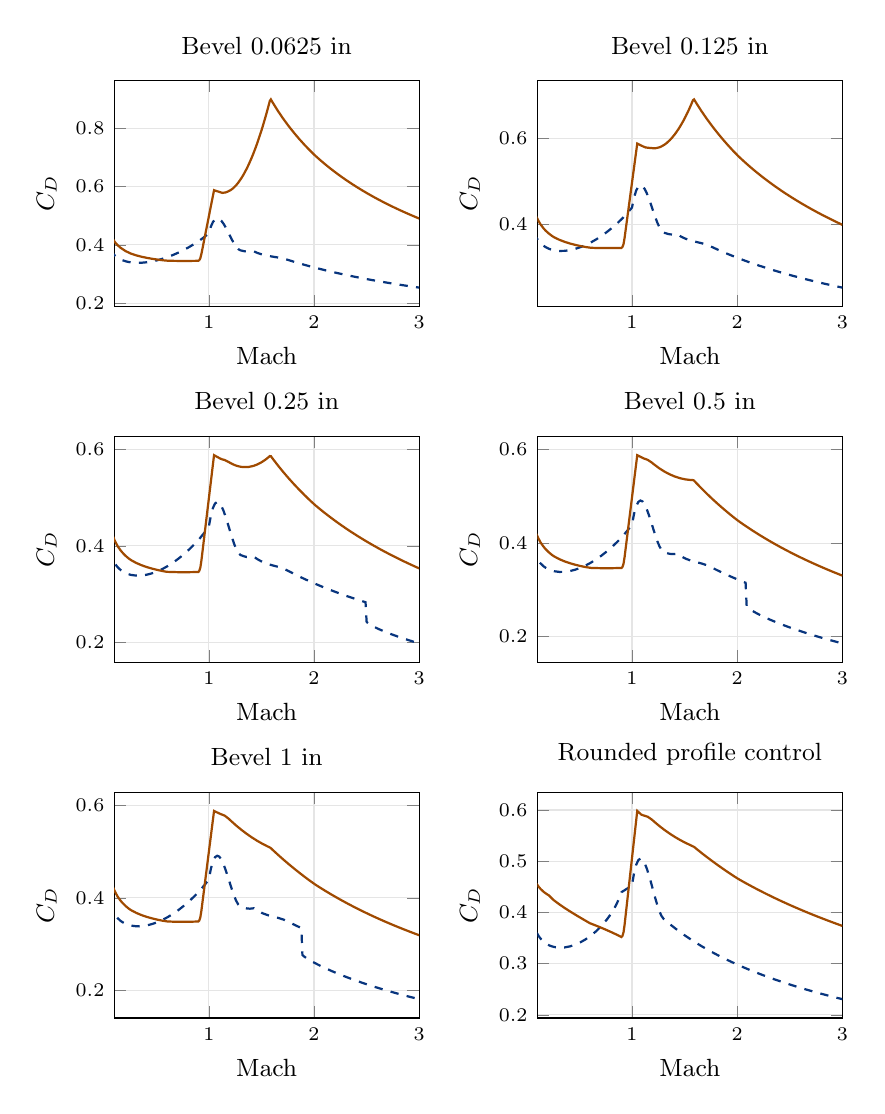
\begin{tikzpicture}
\begin{groupplot}[group style={group size=2 by 3,horizontal sep=1.50cm,vertical sep=1.65cm},width=.45\textwidth,height=4.45cm,grid=major,grid style={gray!20},tick label style={font=\scriptsize},label style={font=\small},title style={font=\small},scaled y ticks=false,yticklabel style={/pgf/number format/fixed,/pgf/number format/precision=3},unbounded coords=jump]
\nextgroupplot[title={Bevel 0.0625 in},xlabel={Mach},ylabel={$C_D$},xmin=0.1,xmax=3]
\addplot[thick,B,dashed] coordinates {(0.01,0.4955621) (0.02,0.4463415) (0.03,0.4221597) (0.04,0.4067373) (0.05,0.3956786) (0.06,0.3872002) (0.07,0.3804143) (0.08,0.3748193) (0.09,0.3701059) (0.1,0.3660711) (0.11,0.3625749) (0.13,0.3568235) (0.14,0.354438) (0.16,0.3504259) (0.18,0.3472289) (0.21,0.3436136) (0.23,0.3418356) (0.26,0.3399392) (0.31,0.3384548) (0.36,0.3386713) (0.41,0.3403069) (0.46,0.3431862) (0.51,0.3471947) (0.56,0.3522544) (0.61,0.3583117) (0.66,0.3653296) (0.71,0.3732834) (0.76,0.3821579) (0.81,0.3919458) (0.86,0.4026476) (0.91,0.4144078) (0.96,0.4277726) (1,0.4393144) (1.01,0.4510799) (1.02,0.4629209) (1.04,0.4788217) (1.06,0.4878998) (1.08,0.4910396) (1.1,0.4891272) (1.11,0.4858248) (1.12,0.4825817) (1.14,0.4727157) (1.16,0.4604176) (1.18,0.4465782) (1.21,0.4249381) (1.22,0.4178484) (1.24,0.404751) (1.26,0.3936996) (1.28,0.3856) (1.3,0.3813638) (1.31,0.3804075) (1.34,0.37809) (1.36,0.3770685) (1.39,0.3764987) (1.41,0.376916) (1.43,0.3775066) (1.46,0.3727592) (1.48,0.3700851) (1.51,0.366726) (1.56,0.3625256) (1.61,0.3594235) (1.66,0.3565539) (1.71,0.3529445) (1.76,0.3476781) (1.81,0.342054) (1.86,0.3366609) (1.91,0.3314828) (1.96,0.3265051) (2.01,0.321715) (2.06,0.3171006) (2.11,0.3126512) (2.16,0.3083573) (2.21,0.3042101) (2.26,0.3002013) (2.31,0.2963238) (2.36,0.2925705) (2.41,0.2889353) (2.46,0.2854124) (2.51,0.2819964) (2.56,0.2786823) (2.61,0.2754654) (2.66,0.2723414) (2.71,0.2693063) (2.76,0.2663562) (2.81,0.2634875) (2.86,0.2606971) (2.91,0.2579816) (2.96,0.2553382) (3,0.2532734)};
\addplot[thick,burntorange] coordinates {(0.01,0.5849357) (0.02,0.5200357) (0.03,0.4881231) (0.04,0.4677548) (0.05,0.4531194) (0.06,0.441857) (0.07,0.4327921) (0.08,0.4252609) (0.09,0.4188542) (0.11,0.4084244) (0.13,0.4001842) (0.16,0.3904686) (0.21,0.3785684) (0.26,0.3700168) (0.31,0.3640871) (0.36,0.3593832) (0.41,0.3555447) (0.46,0.3523461) (0.51,0.3496377) (0.56,0.347315) (0.61,0.345589) (0.66,0.3451865) (0.71,0.344961) (0.76,0.3448839) (0.81,0.3449327) (0.86,0.3450892) (0.9,0.3452819) (0.91,0.3476298) (0.92,0.3546736) (0.93,0.3690731) (0.96,0.4237731) (1.01,0.5149398) (1.05,0.5878732) (1.06,0.5866429) (1.11,0.5807182) (1.13,0.5785357) (1.16,0.5802444) (1.18,0.5828607) (1.21,0.5886512) (1.23,0.5940994) (1.26,0.6048362) (1.28,0.6136335) (1.31,0.6292127) (1.33,0.6411593) (1.36,0.6613904) (1.38,0.6764085) (1.41,0.7012244) (1.44,0.728787) (1.46,0.7486918) (1.49,0.7808538) (1.51,0.8038395) (1.54,0.8406513) (1.56,0.8667588) (1.58,0.8941292) (1.59,0.8996861) (1.61,0.8874085) (1.66,0.8585968) (1.71,0.8321241) (1.76,0.8076386) (1.81,0.7848625) (1.86,0.7635737) (1.91,0.7435911) (1.96,0.7247652) (2.01,0.707123) (2.06,0.6909909) (2.11,0.6757009) (2.16,0.6611773) (2.21,0.6473542) (2.26,0.6341745) (2.31,0.6215878) (2.36,0.6095495) (2.41,0.5980195) (2.46,0.5869625) (2.51,0.5763462) (2.56,0.5661413) (2.61,0.5563213) (2.66,0.5468619) (2.71,0.5377407) (2.76,0.528937) (2.81,0.5204314) (2.86,0.5122063) (2.91,0.5042447) (2.96,0.496531) (3,0.4905285)};
\nextgroupplot[title={Bevel 0.125 in},xlabel={Mach},ylabel={$C_D$},xmin=0.1,xmax=3]
\addplot[thick,B,dashed] coordinates {(0.01,0.4955621) (0.02,0.4463415) (0.03,0.4221597) (0.04,0.4067373) (0.05,0.3956786) (0.06,0.3872002) (0.07,0.3804143) (0.08,0.3748193) (0.09,0.3701059) (0.1,0.3660711) (0.11,0.3625749) (0.13,0.3568235) (0.14,0.354438) (0.16,0.3504259) (0.18,0.3472289) (0.21,0.3436136) (0.23,0.3418356) (0.26,0.3399392) (0.31,0.3384548) (0.36,0.3386713) (0.41,0.3403069) (0.46,0.3431862) (0.51,0.3471947) (0.56,0.3522544) (0.61,0.3583117) (0.66,0.3653296) (0.71,0.3732834) (0.76,0.3821579) (0.81,0.3919458) (0.86,0.4026476) (0.91,0.4144078) (0.96,0.4277726) (1,0.4393144) (1.01,0.4510799) (1.02,0.4629209) (1.04,0.4788217) (1.06,0.4878998) (1.08,0.4910396) (1.1,0.4891272) (1.11,0.4858248) (1.12,0.4825817) (1.14,0.4727157) (1.16,0.4604176) (1.18,0.4465782) (1.21,0.4249381) (1.22,0.4178484) (1.24,0.404751) (1.26,0.3936996) (1.28,0.3856) (1.3,0.3813638) (1.31,0.3804075) (1.34,0.37809) (1.36,0.3770685) (1.39,0.3764987) (1.41,0.376916) (1.43,0.3775066) (1.46,0.3727592) (1.48,0.3700851) (1.51,0.366726) (1.56,0.3625256) (1.61,0.3594235) (1.66,0.3565539) (1.71,0.3529445) (1.76,0.3476781) (1.81,0.342054) (1.86,0.3366609) (1.91,0.3314828) (1.96,0.3265051) (2.01,0.321715) (2.06,0.3171006) (2.11,0.3126512) (2.16,0.3083573) (2.21,0.3042101) (2.26,0.3002013) (2.31,0.2963238) (2.36,0.2925705) (2.41,0.2889353) (2.46,0.2854124) (2.51,0.2819964) (2.56,0.2786823) (2.61,0.2754654) (2.66,0.2723414) (2.71,0.2693063) (2.76,0.2663562) (2.81,0.2634875) (2.86,0.2606971) (2.91,0.2579816) (2.96,0.2553382) (3,0.2532734)};
\addplot[thick,burntorange] coordinates {(0.01,0.5853934) (0.02,0.5204212) (0.03,0.4884735) (0.04,0.468083) (0.05,0.4534317) (0.06,0.4421571) (0.07,0.4330823) (0.08,0.4255429) (0.09,0.4191294) (0.11,0.4086882) (0.13,0.4004391) (0.16,0.390713) (0.18,0.3854422) (0.21,0.3788) (0.24,0.3732712) (0.26,0.3702394) (0.31,0.3643047) (0.36,0.359597) (0.41,0.3557556) (0.46,0.3525548) (0.51,0.3498445) (0.56,0.3475205) (0.61,0.3457941) (0.66,0.3453943) (0.71,0.3451717) (0.76,0.3450976) (0.81,0.3451494) (0.86,0.345309) (0.9,0.3455043) (0.91,0.3478537) (0.92,0.354902) (0.93,0.3692956) (0.96,0.42394) (1.01,0.515014) (1.05,0.5878732) (1.06,0.5866429) (1.11,0.5807182) (1.13,0.5787605) (1.16,0.577955) (1.21,0.576932) (1.23,0.5772854) (1.26,0.5791277) (1.28,0.5811981) (1.31,0.585531) (1.33,0.5892238) (1.36,0.5959542) (1.38,0.6012299) (1.41,0.6103221) (1.44,0.6208274) (1.46,0.628617) (1.49,0.6414847) (1.51,0.650855) (1.54,0.6661057) (1.56,0.6770742) (1.58,0.6886882) (1.59,0.6904686) (1.61,0.6824393) (1.66,0.6634052) (1.71,0.6456751) (1.76,0.6290669) (1.81,0.6134359) (1.86,0.5986658) (1.91,0.5846608) (1.96,0.5713415) (2.01,0.5587927) (2.06,0.547389) (2.11,0.5365031) (2.16,0.5260941) (2.21,0.5161255) (2.26,0.506566) (2.31,0.497387) (2.36,0.4885636) (2.41,0.4800724) (2.46,0.4718932) (2.51,0.4640068) (2.56,0.4563958) (2.61,0.4490441) (2.66,0.4419368) (2.71,0.43506) (2.76,0.4284005) (2.81,0.421946) (2.86,0.4156848) (2.91,0.409606) (2.96,0.4036988) (3,0.3990901)};
\nextgroupplot[title={Bevel 0.25 in},xlabel={Mach},ylabel={$C_D$},xmin=0.1,xmax=3]
\addplot[thick,B,dashed] coordinates {(0.01,0.4955621) (0.02,0.4463415) (0.03,0.4221597) (0.04,0.4067373) (0.05,0.3956786) (0.06,0.3872002) (0.07,0.3804143) (0.08,0.3748193) (0.09,0.3701059) (0.11,0.3625749) (0.13,0.3568235) (0.16,0.3504259) (0.18,0.3472289) (0.21,0.3436136) (0.23,0.3418356) (0.26,0.3399392) (0.31,0.3384548) (0.36,0.3386713) (0.41,0.3403069) (0.46,0.3431862) (0.51,0.3471947) (0.56,0.3522544) (0.61,0.3583117) (0.66,0.3653296) (0.71,0.3732834) (0.76,0.3821579) (0.81,0.3919458) (0.86,0.4026476) (0.91,0.4144078) (0.96,0.4277726) (1,0.4393144) (1.01,0.4510799) (1.02,0.4629209) (1.04,0.4788217) (1.06,0.4878998) (1.08,0.4910396) (1.1,0.4891272) (1.11,0.4858248) (1.12,0.4825817) (1.14,0.4727157) (1.16,0.4604176) (1.18,0.4465782) (1.21,0.4249381) (1.22,0.4178484) (1.24,0.404751) (1.26,0.3936996) (1.28,0.3856) (1.3,0.3813638) (1.31,0.3804075) (1.34,0.37809) (1.36,0.3770685) (1.39,0.3764987) (1.41,0.376916) (1.43,0.3775066) (1.46,0.3727592) (1.51,0.366726) (1.56,0.3625256) (1.61,0.3594235) (1.66,0.3565539) (1.71,0.3529445) (1.76,0.3476781) (1.81,0.342054) (1.86,0.3366609) (1.91,0.3314828) (1.96,0.3265051) (2.01,0.321715) (2.06,0.3171006) (2.11,0.3126512) (2.16,0.3083573) (2.21,0.3042101) (2.26,0.3002013) (2.31,0.2963238) (2.36,0.2925705) (2.41,0.2889353) (2.46,0.2854124) (2.49,0.2833503) (2.5,0.2430483) (2.51,0.240604) (2.53,0.2374095) (2.56,0.233615) (2.61,0.2282684) (2.66,0.2235344) (2.71,0.2191793) (2.76,0.2151014) (2.81,0.2112445) (2.86,0.2075729) (2.91,0.2040619) (2.96,0.2006932) (3,0.1980912)};
\addplot[thick,burntorange] coordinates {(0.01,0.5863164) (0.02,0.5211986) (0.03,0.4891801) (0.04,0.4687447) (0.05,0.4540613) (0.06,0.442762) (0.07,0.4336675) (0.08,0.4261116) (0.09,0.4196841) (0.1,0.4141154) (0.11,0.4092202) (0.13,0.4009531) (0.14,0.3974088) (0.16,0.3912058) (0.18,0.3859236) (0.21,0.3792669) (0.24,0.3737261) (0.26,0.3706882) (0.31,0.3647434) (0.36,0.3600281) (0.41,0.3561808) (0.46,0.3529754) (0.51,0.3502616) (0.56,0.3479347) (0.6,0.3463006) (0.61,0.3462077) (0.66,0.3458135) (0.71,0.3455966) (0.76,0.3455285) (0.81,0.3455865) (0.86,0.3457523) (0.9,0.3459527) (0.91,0.3483052) (0.92,0.3553626) (0.93,0.3697444) (0.96,0.4242766) (1.01,0.5151636) (1.05,0.5878732) (1.06,0.5866429) (1.11,0.5807182) (1.13,0.5790303) (1.15,0.5780496) (1.16,0.576851) (1.19,0.5736579) (1.21,0.5710699) (1.23,0.5688669) (1.26,0.5662524) (1.28,0.564955) (1.31,0.5636602) (1.33,0.5632242) (1.36,0.5632031) (1.38,0.5636076) (1.41,0.5648392) (1.43,0.5660756) (1.46,0.5685528) (1.49,0.5717779) (1.51,0.5743443) (1.54,0.5788208) (1.56,0.5822248) (1.58,0.5859661) (1.59,0.5858598) (1.61,0.5799547) (1.66,0.5658094) (1.71,0.5524506) (1.76,0.5397811) (1.81,0.5277226) (1.86,0.5162118) (1.91,0.5051956) (1.96,0.4946296) (2.01,0.4846276) (2.06,0.475588) (2.11,0.4669043) (2.16,0.4585525) (2.21,0.4505112) (2.26,0.4427617) (2.31,0.4352867) (2.36,0.4280706) (2.41,0.4210989) (2.46,0.4143585) (2.51,0.4078372) (2.56,0.4015231) (2.61,0.3954055) (2.66,0.3894743) (2.71,0.3837197) (2.76,0.3781323) (2.81,0.3727032) (2.86,0.3674241) (2.91,0.3622866) (2.96,0.3572828) (3,0.3533708)};
\nextgroupplot[title={Bevel 0.5 in},xlabel={Mach},ylabel={$C_D$},xmin=0.1,xmax=3]
\addplot[thick,B,dashed] coordinates {(0.01,0.4955621) (0.02,0.4463415) (0.03,0.4221597) (0.04,0.4067373) (0.05,0.3956786) (0.06,0.3872002) (0.07,0.3804143) (0.08,0.3748193) (0.09,0.3701059) (0.11,0.3625749) (0.13,0.3568235) (0.16,0.3504259) (0.18,0.3472289) (0.21,0.3436136) (0.26,0.3399392) (0.31,0.3384548) (0.36,0.3386713) (0.41,0.3403069) (0.46,0.3431862) (0.51,0.3471947) (0.56,0.3522544) (0.61,0.3583117) (0.66,0.3653296) (0.71,0.3732834) (0.76,0.3821579) (0.81,0.3919458) (0.86,0.4026476) (0.91,0.4144078) (0.96,0.4277726) (1,0.4393144) (1.01,0.4510799) (1.02,0.4629209) (1.04,0.4788217) (1.06,0.4878998) (1.08,0.4910396) (1.1,0.4891272) (1.11,0.4858248) (1.12,0.4825817) (1.14,0.4727157) (1.16,0.4604176) (1.18,0.4465782) (1.21,0.4249381) (1.22,0.4178484) (1.24,0.404751) (1.26,0.3936996) (1.28,0.3856) (1.3,0.3813638) (1.31,0.3804075) (1.34,0.37809) (1.36,0.3770685) (1.39,0.3764987) (1.41,0.376916) (1.43,0.3775066) (1.46,0.3727592) (1.51,0.366726) (1.56,0.3625256) (1.61,0.3594235) (1.66,0.3565539) (1.71,0.3529445) (1.76,0.3476781) (1.81,0.342054) (1.86,0.3366609) (1.91,0.3314828) (1.96,0.3265051) (2.01,0.321715) (2.06,0.3171006) (2.08,0.3153016) (2.09,0.2652242) (2.1,0.2624953) (2.11,0.260562) (2.16,0.2532077) (2.21,0.2471643) (2.26,0.2417165) (2.31,0.2366627) (2.36,0.231909) (2.41,0.2274012) (2.46,0.2231039) (2.51,0.2189919) (2.56,0.2150461) (2.61,0.2112516) (2.66,0.207596) (2.71,0.2040691) (2.76,0.2006621) (2.81,0.1973672) (2.86,0.1941779) (2.91,0.1910881) (2.96,0.1880924) (3,0.1857603)};
\addplot[thick,burntorange] coordinates {(0.01,0.5881895) (0.02,0.5227761) (0.03,0.4906142) (0.04,0.4700877) (0.05,0.4553391) (0.06,0.4439897) (0.07,0.434855) (0.08,0.4272657) (0.09,0.4208098) (0.1,0.4152166) (0.11,0.4102998) (0.13,0.4019963) (0.14,0.3984364) (0.16,0.3922061) (0.18,0.3869005) (0.21,0.3802145) (0.24,0.3746493) (0.26,0.3715991) (0.31,0.3656338) (0.36,0.3609029) (0.41,0.3570437) (0.46,0.3538291) (0.51,0.351108) (0.56,0.3487754) (0.61,0.347047) (0.66,0.3466641) (0.71,0.346459) (0.76,0.346403) (0.81,0.3464734) (0.86,0.3466519) (0.9,0.3468626) (0.91,0.3492213) (0.92,0.3562973) (0.93,0.3706551) (0.96,0.4249596) (1.01,0.5154671) (1.05,0.5878732) (1.06,0.5866429) (1.11,0.5810118) (1.15,0.5778794) (1.16,0.5763479) (1.19,0.5718315) (1.21,0.5681236) (1.26,0.5597698) (1.31,0.5526653) (1.36,0.5467635) (1.41,0.542037) (1.46,0.5384699) (1.51,0.536054) (1.56,0.5347868) (1.58,0.5346019) (1.59,0.5335555) (1.61,0.5287124) (1.66,0.5170115) (1.71,0.5058384) (1.76,0.4951382) (1.81,0.484866) (1.86,0.4749848) (1.91,0.4654631) (1.96,0.4562737) (2.01,0.447545) (2.06,0.4396875) (2.11,0.4321048) (2.16,0.4247817) (2.21,0.417704) (2.26,0.4108596) (2.31,0.4042365) (2.36,0.3978241) (2.41,0.3916121) (2.46,0.3855912) (2.51,0.3797523) (2.56,0.3740867) (2.61,0.3685863) (2.66,0.363243) (2.71,0.3580495) (2.76,0.3529982) (2.81,0.3480819) (2.86,0.3432938) (2.91,0.3386269) (2.96,0.3340748) (3,0.3305112)};
\nextgroupplot[title={Bevel 1 in},xlabel={Mach},ylabel={$C_D$},xmin=0.1,xmax=3]
\addplot[thick,B,dashed] coordinates {(0.01,0.4955621) (0.02,0.4463415) (0.03,0.4221597) (0.04,0.4067373) (0.05,0.3956786) (0.06,0.3872002) (0.07,0.3804143) (0.08,0.3748193) (0.09,0.3701059) (0.11,0.3625749) (0.13,0.3568235) (0.16,0.3504259) (0.18,0.3472289) (0.21,0.3436136) (0.26,0.3399392) (0.31,0.3384548) (0.36,0.3386713) (0.41,0.3403069) (0.46,0.3431862) (0.51,0.3471947) (0.56,0.3522544) (0.61,0.3583117) (0.66,0.3653296) (0.71,0.3732834) (0.76,0.3821579) (0.81,0.3919458) (0.86,0.4026476) (0.91,0.4144078) (0.96,0.4277726) (1,0.4393144) (1.01,0.4510799) (1.02,0.4629209) (1.04,0.4788217) (1.06,0.4878998) (1.08,0.4910396) (1.1,0.4891272) (1.11,0.4858248) (1.12,0.4825817) (1.14,0.4727157) (1.16,0.4604176) (1.18,0.4465782) (1.21,0.4249381) (1.22,0.4178484) (1.24,0.404751) (1.26,0.3936996) (1.28,0.3856) (1.3,0.3813638) (1.31,0.3804075) (1.36,0.3770685) (1.39,0.3764987) (1.41,0.376916) (1.43,0.3775066) (1.46,0.3727592) (1.51,0.366726) (1.56,0.3625256) (1.61,0.3594235) (1.66,0.3565539) (1.71,0.3529445) (1.76,0.3476781) (1.81,0.342054) (1.86,0.3366609) (1.88,0.3345647) (1.89,0.2762771) (1.91,0.2724443) (1.96,0.2650805) (2.01,0.2587603) (2.06,0.2529753) (2.11,0.2475652) (2.16,0.2424515) (2.21,0.2375876) (2.26,0.2329419) (2.31,0.2284911) (2.36,0.2242172) (2.41,0.2201057) (2.46,0.2161444) (2.51,0.2123229) (2.56,0.2086322) (2.61,0.2050643) (2.66,0.2016122) (2.71,0.1982694) (2.76,0.1950302) (2.81,0.1918893) (2.86,0.1888419) (2.91,0.1858835) (2.96,0.18301) (3,0.1807698)};
\addplot[thick,burntorange] coordinates {(0.01,0.5920161) (0.02,0.525999) (0.03,0.4935439) (0.04,0.4728313) (0.05,0.4579496) (0.06,0.4464979) (0.07,0.437281) (0.08,0.4296236) (0.09,0.4231097) (0.1,0.4174664) (0.11,0.4125055) (0.13,0.4041275) (0.14,0.4005357) (0.16,0.3942495) (0.18,0.3888964) (0.21,0.3821504) (0.24,0.3765352) (0.26,0.3734602) (0.31,0.3674528) (0.36,0.3626903) (0.41,0.3588067) (0.46,0.3555731) (0.51,0.3528371) (0.56,0.3504929) (0.61,0.3487618) (0.66,0.3484019) (0.71,0.3482208) (0.76,0.3481895) (0.81,0.3482854) (0.86,0.3484899) (0.9,0.3487217) (0.91,0.351093) (0.92,0.3582069) (0.93,0.3725156) (0.96,0.426355) (1.01,0.5160873) (1.05,0.5878732) (1.06,0.5866914) (1.11,0.5814496) (1.15,0.5778407) (1.16,0.5761177) (1.19,0.5708856) (1.21,0.5665926) (1.26,0.5564306) (1.31,0.5470513) (1.36,0.5384235) (1.41,0.5305243) (1.46,0.5233363) (1.51,0.5168462) (1.56,0.5110441) (1.58,0.5089142) (1.59,0.5074033) (1.61,0.5030912) (1.66,0.4926125) (1.71,0.4825322) (1.76,0.4728167) (1.81,0.4634376) (1.86,0.4543713) (1.91,0.4455968) (1.96,0.4370958) (2.01,0.4290037) (2.06,0.4217373) (2.11,0.4147051) (2.16,0.4078963) (2.21,0.4013005) (2.26,0.3949085) (2.31,0.3887114) (2.36,0.3827009) (2.41,0.3768687) (2.46,0.3712076) (2.51,0.3657099) (2.56,0.3603685) (2.61,0.3551766) (2.66,0.3501274) (2.71,0.3452144) (2.76,0.3404311) (2.81,0.3357712) (2.86,0.3312286) (2.91,0.3267971) (2.96,0.3224707) (3,0.3190814)};
\nextgroupplot[title={Rounded profile control},xlabel={Mach},ylabel={$C_D$},xmin=0.1,xmax=3]
\addplot[thick,B,dashed] coordinates {(0.01,0.4878037) (0.02,0.4385845) (0.03,0.4144049) (0.04,0.3989857) (0.05,0.3879311) (0.06,0.3794578) (0.07,0.3726779) (0.08,0.3670899) (0.09,0.3623844) (0.11,0.3548726) (0.13,0.3491446) (0.16,0.3427912) (0.18,0.3396301) (0.21,0.3360796) (0.23,0.334353) (0.26,0.3325476) (0.31,0.3312587) (0.36,0.3317401) (0.41,0.3337318) (0.46,0.3370885) (0.51,0.3417371) (0.56,0.3476591) (0.61,0.3548874) (0.66,0.363516) (0.71,0.3737295) (0.76,0.3858688) (0.79,0.3943283) (0.81,0.4005931) (0.84,0.4112008) (0.86,0.419333) (0.88,0.4286412) (0.89,0.4338769) (0.9,0.4396765) (0.91,0.4408726) (0.96,0.4474003) (1,0.453289) (1.01,0.4651485) (1.02,0.4770658) (1.04,0.493064) (1.06,0.502163) (1.08,0.5052436) (1.1,0.5031876) (1.11,0.4997802) (1.12,0.4964091) (1.14,0.4862149) (1.16,0.4734866) (1.18,0.4591068) (1.21,0.4364276) (1.22,0.4289246) (1.24,0.4148895) (1.26,0.4027373) (1.28,0.3933526) (1.3,0.3876203) (1.31,0.3858267) (1.36,0.3771863) (1.41,0.3690517) (1.46,0.3613688) (1.51,0.3540941) (1.56,0.3471887) (1.61,0.3406202) (1.66,0.3343598) (1.71,0.3283825) (1.76,0.3226662) (1.81,0.3171914) (1.86,0.3119407) (1.91,0.3068986) (1.96,0.3020511) (2.01,0.2973858) (2.06,0.2928911) (2.11,0.288557) (2.16,0.2843739) (2.21,0.2803334) (2.26,0.2764276) (2.31,0.2726494) (2.36,0.2689921) (2.41,0.2654497) (2.46,0.2620166) (2.51,0.2586874) (2.56,0.2554574) (2.61,0.252322) (2.66,0.249277) (2.71,0.2463185) (2.76,0.2434428) (2.81,0.2406464) (2.86,0.2379261) (2.91,0.2352788) (2.96,0.2327016) (3,0.2306885)};
\addplot[thick,burntorange] coordinates {(0.01,0.554368) (0.02,0.5167136) (0.03,0.498033) (0.04,0.4860594) (0.05,0.4774342) (0.06,0.470786) (0.07,0.4654289) (0.08,0.4609746) (0.09,0.4571834) (0.11,0.4510079) (0.13,0.446127) (0.16,0.4403714) (0.18,0.4372525) (0.21,0.4333231) (0.25,0.4251324) (0.26,0.4234909) (0.31,0.4158165) (0.36,0.4087864) (0.41,0.4021798) (0.46,0.3958579) (0.51,0.3897286) (0.56,0.3837276) (0.6,0.3789875) (0.61,0.3782149) (0.66,0.3741837) (0.71,0.3699769) (0.76,0.3655739) (0.81,0.3609587) (0.86,0.3561179) (0.9,0.3520757) (0.91,0.3544698) (0.92,0.3616521) (0.93,0.3762873) (0.96,0.4317779) (1.01,0.5242623) (1.05,0.5982497) (1.06,0.5963754) (1.09,0.5908795) (1.11,0.5894698) (1.15,0.5869077) (1.16,0.5854805) (1.19,0.581165) (1.21,0.5774913) (1.26,0.5688664) (1.31,0.560975) (1.36,0.5537616) (1.41,0.5471864) (1.46,0.5412197) (1.51,0.5358377) (1.56,0.5310222) (1.59,0.5280377) (1.61,0.5246526) (1.66,0.516407) (1.71,0.5084454) (1.76,0.5007401) (1.81,0.4932681) (1.86,0.4860105) (1.91,0.4789507) (1.96,0.4720746) (2.01,0.4655202) (2.06,0.4597047) (2.11,0.4540472) (2.16,0.4485407) (2.21,0.4431783) (2.26,0.4379543) (2.31,0.4328632) (2.36,0.4279001) (2.41,0.4230597) (2.46,0.4183376) (2.51,0.4137295) (2.56,0.4092306) (2.61,0.404837) (2.66,0.4005442) (2.71,0.3963483) (2.76,0.3922448) (2.81,0.3882297) (2.86,0.3842988) (2.91,0.3804479) (2.96,0.3766726) (3,0.3737042)};
\end{groupplot}\end{tikzpicture}
\caption{FX1 is measured parallel to the body. Maximum thickness is 0.125 in and the trailing edge remains blunt.}\label{fig:atlas-09-bevel-length}
\end{figure}
\noindent{\footnotesize Export files: \code{09-bevel-length.svg} and \code{09-bevel-length.png}.\\ Directory: \code{aerodynamic-investigation/extended/figures/}.}

\clearpage\subsubsection*{Square fin sweep}
\begin{figure}[H]\centering
{\footnotesize\begin{tabular}{ll}
\tikz[baseline=-.5ex]{\draw[thick,B,dashed] (0,0)--(.40,0);}\ MIT OR & \tikz[baseline=-.5ex]{\draw[thick,burntorange] (0,0)--(.40,0);}\ RASAero\\
\end{tabular}}\par\vspace{.7em}
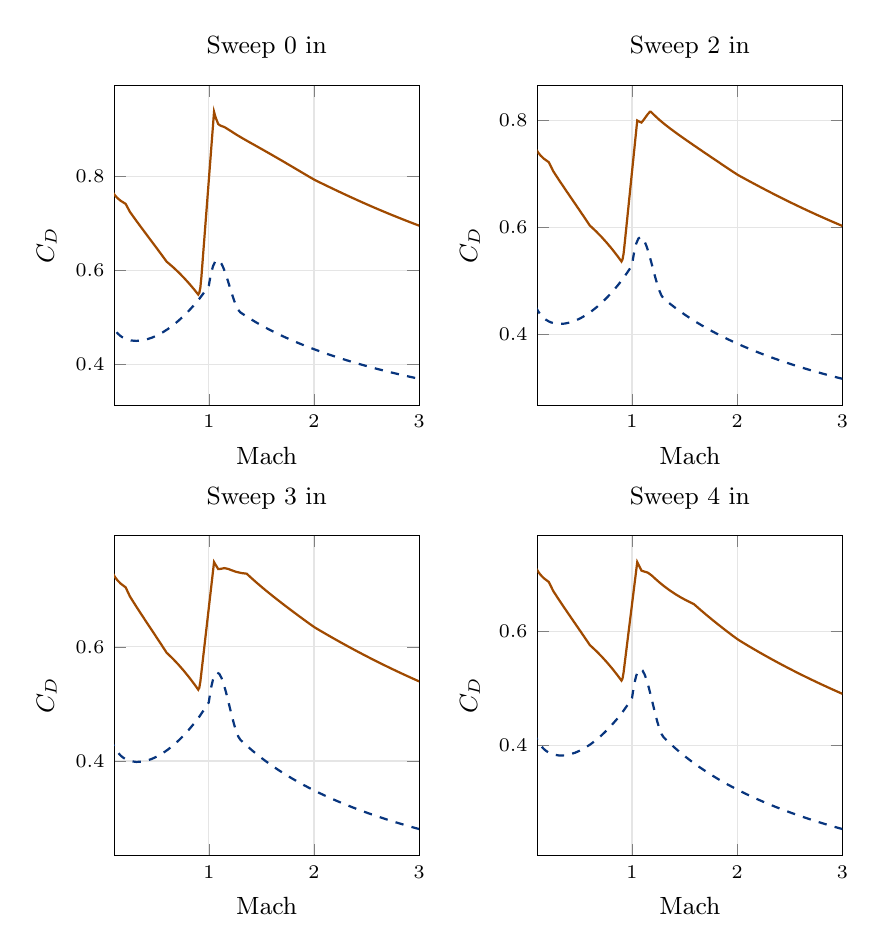
\begin{tikzpicture}
\begin{groupplot}[group style={group size=2 by 2,horizontal sep=1.50cm,vertical sep=1.65cm},width=.45\textwidth,height=5.65cm,grid=major,grid style={gray!20},tick label style={font=\scriptsize},label style={font=\small},title style={font=\small},scaled y ticks=false,yticklabel style={/pgf/number format/fixed,/pgf/number format/precision=3},unbounded coords=jump]
\nextgroupplot[title={Sweep 0 in},xlabel={Mach},ylabel={$C_D$},xmin=0.1,xmax=3]
\addplot[thick,B,dashed] coordinates {(0.01,0.6054804) (0.02,0.5562654) (0.03,0.5320931) (0.04,0.516684) (0.05,0.5056423) (0.06,0.4971848) (0.07,0.4904236) (0.08,0.484857) (0.09,0.4801758) (0.1,0.476177) (0.11,0.4727206) (0.13,0.4670603) (0.14,0.4647259) (0.16,0.4608277) (0.18,0.4577597) (0.21,0.4543663) (0.23,0.4527554) (0.26,0.4511381) (0.31,0.450195) (0.36,0.451048) (0.41,0.453415) (0.46,0.4571206) (0.51,0.4620491) (0.56,0.4681217) (0.61,0.4752828) (0.66,0.4834926) (0.71,0.4927225) (0.76,0.5029517) (0.81,0.5141653) (0.86,0.526353) (0.91,0.5396449) (0.96,0.5545667) (1,0.5673541) (1.01,0.5801353) (1.02,0.5923233) (1.04,0.6088833) (1.06,0.6185645) (1.08,0.6222403) (1.1,0.6207864) (1.11,0.6176812) (1.12,0.6146123) (1.14,0.605021) (1.16,0.592891) (1.18,0.5791024) (1.21,0.5572927) (1.22,0.5500743) (1.24,0.5365994) (1.26,0.5249949) (1.28,0.5161448) (1.3,0.5109336) (1.31,0.5093955) (1.36,0.5019799) (1.41,0.4949836) (1.46,0.4883551) (1.51,0.4820549) (1.56,0.4760491) (1.61,0.4703107) (1.66,0.4648159) (1.71,0.459545) (1.76,0.4544808) (1.81,0.4496082) (1.86,0.4449141) (1.91,0.4403869) (1.96,0.436016) (2.01,0.4317923) (2.06,0.4277073) (2.11,0.4237534) (2.16,0.4199236) (2.21,0.4162118) (2.26,0.4126119) (2.31,0.4091187) (2.36,0.4057273) (2.41,0.402433) (2.46,0.3992317) (2.51,0.3961192) (2.56,0.393092) (2.61,0.3901465) (2.66,0.3872795) (2.71,0.3844879) (2.76,0.3817688) (2.81,0.3791195) (2.86,0.3765374) (2.91,0.3740201) (2.96,0.3715653) (3,0.3696449)};
\addplot[thick,burntorange] coordinates {(0.01,0.8625659) (0.02,0.8249114) (0.03,0.8062309) (0.04,0.7942572) (0.05,0.7856321) (0.06,0.7789838) (0.07,0.7736267) (0.08,0.7691725) (0.09,0.7653812) (0.11,0.7592058) (0.13,0.7543249) (0.16,0.7485692) (0.21,0.741521) (0.25,0.7247727) (0.26,0.7215813) (0.31,0.70601) (0.36,0.6908386) (0.41,0.6758465) (0.46,0.6608949) (0.51,0.6458917) (0.56,0.6307722) (0.6,0.6185616) (0.61,0.6167782) (0.66,0.6071318) (0.71,0.5966393) (0.76,0.5852802) (0.81,0.5730383) (0.86,0.5599002) (0.9,0.5487375) (0.91,0.5524689) (0.92,0.5636631) (0.93,0.5866675) (0.96,0.6743197) (1.01,0.8204067) (1.05,0.9372762) (1.06,0.9291639) (1.07,0.9223837) (1.09,0.9112706) (1.11,0.9081227) (1.15,0.9047689) (1.16,0.9033992) (1.21,0.8963871) (1.26,0.889134) (1.31,0.882461) (1.36,0.8760588) (1.41,0.8697651) (1.46,0.8634923) (1.51,0.8571938) (1.56,0.850847) (1.61,0.844444) (1.66,0.8379851) (1.71,0.8314757) (1.76,0.8249244) (1.81,0.8183408) (1.86,0.8117355) (1.91,0.8051185) (1.96,0.7984993) (2.01,0.792121) (2.06,0.7866607) (2.11,0.7812345) (2.16,0.7758506) (2.21,0.7705155) (2.26,0.7652358) (2.31,0.7600163) (2.36,0.7548613) (2.41,0.749774) (2.46,0.7447572) (2.51,0.7398129) (2.56,0.7349421) (2.61,0.7301457) (2.66,0.7254239) (2.71,0.7207763) (2.76,0.7162022) (2.81,0.7117005) (2.86,0.7072696) (2.91,0.7029078) (2.96,0.6986128) (3,0.6952235)};
\nextgroupplot[title={Sweep 2 in},xlabel={Mach},ylabel={$C_D$},xmin=0.1,xmax=3]
\addplot[thick,B,dashed] coordinates {(0.01,0.575288) (0.02,0.5260708) (0.03,0.5018947) (0.04,0.4864803) (0.05,0.4754318) (0.06,0.466966) (0.07,0.460195) (0.08,0.454617) (0.09,0.449923) (0.1,0.4459098) (0.11,0.4424376) (0.13,0.4367409) (0.16,0.4304424) (0.18,0.4273227) (0.21,0.4238404) (0.23,0.4221624) (0.26,0.4204328) (0.31,0.419271) (0.36,0.4198654) (0.41,0.4219333) (0.46,0.425298) (0.51,0.4298432) (0.56,0.4354888) (0.61,0.442178) (0.66,0.4498699) (0.71,0.4585342) (0.76,0.4681486) (0.81,0.4786966) (0.86,0.4901661) (0.91,0.5026852) (0.96,0.5167778) (1,0.5288598) (1.01,0.5412645) (1.02,0.5532569) (1.04,0.569426) (1.06,0.5787187) (1.08,0.5820101) (1.1,0.5801775) (1.11,0.5768854) (1.12,0.5736314) (1.14,0.5636755) (1.16,0.5511891) (1.18,0.5370525) (1.21,0.5147376) (1.22,0.5073552) (1.24,0.4935593) (1.26,0.4816428) (1.28,0.4724898) (1.3,0.4669846) (1.31,0.4653028) (1.36,0.4572011) (1.41,0.44957) (1.46,0.4423549) (1.51,0.4355126) (1.56,0.4290057) (1.61,0.4228036) (1.66,0.4168797) (1.71,0.4112111) (1.76,0.4057778) (1.81,0.4005626) (1.86,0.3955497) (1.91,0.3907257) (1.96,0.3860781) (2.01,0.3815961) (2.06,0.3772697) (2.11,0.3730899) (2.16,0.3690484) (2.21,0.365138) (2.26,0.3613517) (2.31,0.3576833) (2.36,0.3541268) (2.41,0.3506771) (2.46,0.3473291) (2.51,0.3440783) (2.56,0.3409202) (2.61,0.3378509) (2.66,0.3348667) (2.71,0.3319641) (2.76,0.3291396) (2.81,0.3263903) (2.86,0.3237132) (2.91,0.3211056) (2.96,0.3185647) (3,0.3165785)};
\addplot[thick,burntorange] coordinates {(0.01,0.8427691) (0.02,0.8051146) (0.03,0.786434) (0.04,0.7744604) (0.05,0.7658353) (0.06,0.759187) (0.07,0.7538299) (0.08,0.7493757) (0.09,0.7455844) (0.11,0.739409) (0.13,0.7345281) (0.16,0.7287724) (0.21,0.7217242) (0.25,0.7055254) (0.26,0.7024337) (0.31,0.6873695) (0.36,0.6727212) (0.41,0.6582678) (0.46,0.6438705) (0.51,0.6294372) (0.56,0.6149035) (0.6,0.6031728) (0.61,0.6014543) (0.66,0.5921687) (0.71,0.5820798) (0.76,0.5711675) (0.81,0.5594154) (0.86,0.5468104) (0.9,0.536105) (0.91,0.5397505) (0.92,0.550687) (0.93,0.5685274) (0.96,0.6263556) (1.01,0.7227359) (1.05,0.7998401) (1.06,0.798663) (1.09,0.7959477) (1.11,0.800783) (1.15,0.8117591) (1.16,0.8138711) (1.17,0.8160558) (1.18,0.8160316) (1.21,0.8102545) (1.26,0.8011407) (1.31,0.7929333) (1.36,0.7852803) (1.41,0.7779799) (1.46,0.7709078) (1.51,0.7639848) (1.56,0.7571595) (1.61,0.750399) (1.66,0.743682) (1.71,0.7369957) (1.76,0.7303333) (1.81,0.7236916) (1.86,0.7170704) (1.91,0.7104707) (1.96,0.703895) (2.01,0.69758) (2.06,0.6921982) (2.11,0.6868615) (2.16,0.681575) (2.21,0.6763427) (2.26,0.6711689) (2.31,0.6660569) (2.36,0.6610097) (2.41,0.6560294) (2.46,0.6511182) (2.51,0.6462772) (2.56,0.6415072) (2.61,0.6368087) (2.66,0.6321816) (2.71,0.6276255) (2.76,0.6231396) (2.81,0.6187226) (2.86,0.6143731) (2.91,0.6100893) (2.96,0.6058692) (3,0.6025374)};
\nextgroupplot[title={Sweep 3 in},xlabel={Mach},ylabel={$C_D$},xmin=0.1,xmax=3]
\addplot[thick,B,dashed] coordinates {(0.01,0.5549106) (0.02,0.5056918) (0.03,0.4815132) (0.04,0.4660952) (0.05,0.4550422) (0.06,0.4465707) (0.07,0.4397931) (0.08,0.4342074) (0.09,0.4295047) (0.11,0.4219989) (0.13,0.4162777) (0.16,0.4099347) (0.18,0.4067802) (0.21,0.4032378) (0.23,0.4015145) (0.26,0.3997092) (0.31,0.3983998) (0.36,0.3988197) (0.41,0.4006856) (0.46,0.4038204) (0.51,0.4081068) (0.56,0.4134642) (0.61,0.419835) (0.66,0.4271772) (0.71,0.4354598) (0.76,0.4446593) (0.81,0.454758) (0.86,0.4657428) (0.91,0.4777404) (0.96,0.4912733) (1,0.5028792) (1.01,0.5150298) (1.02,0.5268901) (1.04,0.5427955) (1.06,0.551826) (1.08,0.554858) (1.1,0.5527698) (1.11,0.5493515) (1.12,0.5459726) (1.14,0.5357706) (1.16,0.5230436) (1.18,0.5086722) (1.21,0.4860163) (1.22,0.4785232) (1.24,0.4645106) (1.26,0.4523836) (1.28,0.4430262) (1.3,0.4373226) (1.31,0.4355437) (1.36,0.4269789) (1.41,0.4189195) (1.46,0.4113085) (1.51,0.4041002) (1.56,0.3972551) (1.61,0.3907402) (1.66,0.3845266) (1.71,0.3785896) (1.76,0.3729073) (1.81,0.3674607) (1.86,0.3622327) (1.91,0.3572084) (1.96,0.352374) (2.01,0.3477177) (2.06,0.3432283) (2.11,0.338896) (2.16,0.3347118) (2.21,0.3306673) (2.26,0.3267552) (2.31,0.3229684) (2.36,0.3193006) (2.41,0.315746) (2.46,0.312299) (2.51,0.3089547) (2.56,0.3057084) (2.61,0.3025556) (2.66,0.2994923) (2.71,0.2965147) (2.76,0.2936192) (2.81,0.2908024) (2.86,0.2880611) (2.91,0.2853925) (2.96,0.2827936) (3,0.2807629)};
\addplot[thick,burntorange] coordinates {(0.01,0.8253413) (0.02,0.7876869) (0.03,0.7690063) (0.04,0.7570327) (0.05,0.7484075) (0.06,0.7417593) (0.07,0.7364022) (0.08,0.7319479) (0.09,0.7281567) (0.11,0.7219813) (0.13,0.7171003) (0.16,0.7113447) (0.21,0.7042964) (0.25,0.6885818) (0.26,0.6855774) (0.31,0.67096) (0.36,0.656772) (0.41,0.6427928) (0.46,0.6288834) (0.51,0.6149519) (0.56,0.6009338) (0.6,0.5896256) (0.61,0.5879643) (0.66,0.578996) (0.71,0.5692626) (0.76,0.5587437) (0.81,0.547423) (0.86,0.5352871) (0.9,0.5249845) (0.91,0.5285544) (0.92,0.5392641) (0.96,0.6036624) (1.01,0.6841853) (1.05,0.7486037) (1.06,0.7453812) (1.09,0.7363511) (1.11,0.7367203) (1.15,0.7380792) (1.16,0.7376404) (1.19,0.736351) (1.21,0.734756) (1.26,0.7315592) (1.31,0.7294317) (1.36,0.7283193) (1.41,0.7198855) (1.46,0.711715) (1.51,0.7038593) (1.56,0.6962489) (1.61,0.6888333) (1.66,0.6815751) (1.71,0.6744463) (1.76,0.6674265) (1.81,0.6605003) (1.86,0.6536566) (1.91,0.646887) (1.96,0.6401856) (2.01,0.6337821) (2.06,0.6283425) (2.11,0.6229738) (2.16,0.6176762) (2.21,0.6124501) (2.26,0.6072963) (2.31,0.6022156) (2.36,0.5972085) (2.41,0.5922753) (2.46,0.5874163) (2.51,0.5826316) (2.56,0.5779206) (2.61,0.5732831) (2.66,0.568718) (2.71,0.5642244) (2.76,0.559801) (2.81,0.555446) (2.86,0.5511579) (2.91,0.5469344) (2.96,0.5427733) (3,0.5394877)};
\nextgroupplot[title={Sweep 4 in},xlabel={Mach},ylabel={$C_D$},xmin=0.1,xmax=3]
\addplot[thick,B,dashed] coordinates {(0.01,0.5392703) (0.02,0.4900503) (0.03,0.4658697) (0.04,0.450449) (0.05,0.4393925) (0.06,0.4309168) (0.07,0.424134) (0.08,0.4185425) (0.09,0.4138331) (0.11,0.4063117) (0.13,0.4005716) (0.16,0.3941944) (0.18,0.3910132) (0.21,0.3874247) (0.23,0.3856667) (0.26,0.3838032) (0.31,0.3823806) (0.36,0.3826665) (0.41,0.3843774) (0.46,0.3873356) (0.51,0.3914235) (0.56,0.3965597) (0.61,0.4026861) (0.66,0.40976) (0.71,0.4177495) (0.76,0.4266305) (0.81,0.4363845) (0.86,0.4469972) (0.91,0.4585945) (0.96,0.4716979) (1,0.4829383) (1.01,0.4948939) (1.02,0.5066529) (1.04,0.5223558) (1.06,0.531185) (1.08,0.5340179) (1.1,0.5317335) (1.11,0.5282184) (1.12,0.5247436) (1.14,0.5143528) (1.16,0.5014411) (1.18,0.4868895) (1.21,0.4639718) (1.22,0.4563939) (1.24,0.442215) (1.26,0.4299264) (1.28,0.420412) (1.3,0.4145561) (1.31,0.4127028) (1.36,0.4037825) (1.41,0.3953943) (1.46,0.3874794) (1.51,0.3799903) (1.56,0.3728856) (1.61,0.3661305) (1.66,0.3596946) (1.71,0.3535516) (1.76,0.3476781) (1.81,0.342054) (1.86,0.3366609) (1.91,0.3314828) (1.96,0.3265051) (2.01,0.321715) (2.06,0.3171006) (2.11,0.3126512) (2.16,0.3083573) (2.21,0.3042101) (2.26,0.3002013) (2.31,0.2963238) (2.36,0.2925705) (2.41,0.2889353) (2.46,0.2854124) (2.51,0.2819964) (2.56,0.2786823) (2.61,0.2754654) (2.66,0.2723414) (2.71,0.2693063) (2.76,0.2663562) (2.81,0.2634875) (2.86,0.2606971) (2.91,0.2579816) (2.96,0.2553382) (3,0.2532734)};
\addplot[thick,burntorange] coordinates {(0.01,0.8080247) (0.02,0.7703703) (0.03,0.7516897) (0.04,0.7397161) (0.05,0.7310909) (0.06,0.7244427) (0.07,0.7190856) (0.08,0.7146313) (0.09,0.71084) (0.11,0.7046646) (0.13,0.6997837) (0.16,0.6940281) (0.21,0.6869798) (0.25,0.6717458) (0.26,0.6688288) (0.31,0.6546548) (0.36,0.6409243) (0.41,0.6274162) (0.46,0.6139917) (0.51,0.6005588) (0.56,0.5870533) (0.6,0.5761646) (0.61,0.5745601) (0.66,0.5659074) (0.71,0.5565273) (0.76,0.5463991) (0.81,0.5355068) (0.86,0.5238373) (0.9,0.5139346) (0.91,0.5174294) (0.92,0.5279136) (0.96,0.5879089) (1.01,0.6623833) (1.05,0.7219628) (1.06,0.7181847) (1.09,0.7070495) (1.11,0.7057831) (1.15,0.7035359) (1.16,0.7021903) (1.19,0.6981246) (1.21,0.6946208) (1.26,0.6864266) (1.31,0.6789658) (1.36,0.6721722) (1.41,0.6659967) (1.46,0.660401) (1.51,0.6553543) (1.56,0.6508322) (1.59,0.6480014) (1.61,0.644709) (1.66,0.6366592) (1.71,0.6288397) (1.76,0.6212208) (1.81,0.6137783) (1.86,0.6064927) (1.91,0.5993475) (1.96,0.5923293) (2.01,0.5856607) (2.06,0.5800016) (2.11,0.5744531) (2.16,0.5690102) (2.21,0.5636688) (2.26,0.5584257) (2.31,0.5532778) (2.36,0.5482225) (2.41,0.5432574) (2.46,0.5383803) (2.51,0.533589) (2.56,0.5288813) (2.61,0.5242552) (2.66,0.5197083) (2.71,0.5152385) (2.76,0.5108433) (2.81,0.5065202) (2.86,0.5022668) (2.91,0.4980803) (2.96,0.4939578) (3,0.4907041)};
\end{groupplot}\end{tikzpicture}
\caption{Root/tip chords, span and thickness are fixed. Leading-edge sweep distance varies without fin overhang past the body.}\label{fig:atlas-10-Hsq-sweep}
\end{figure}
\noindent{\footnotesize Export files: \code{10-Hsq-sweep.svg} and \code{10-Hsq-sweep.png}.\\ Directory: \code{aerodynamic-investigation/extended/figures/}.}

\clearpage\subsubsection*{Beveled fin sweep}
\begin{figure}[H]\centering
{\footnotesize\begin{tabular}{ll}
\tikz[baseline=-.5ex]{\draw[thick,B,dashed] (0,0)--(.40,0);}\ MIT OR & \tikz[baseline=-.5ex]{\draw[thick,burntorange] (0,0)--(.40,0);}\ RASAero\\
\end{tabular}}\par\vspace{.7em}
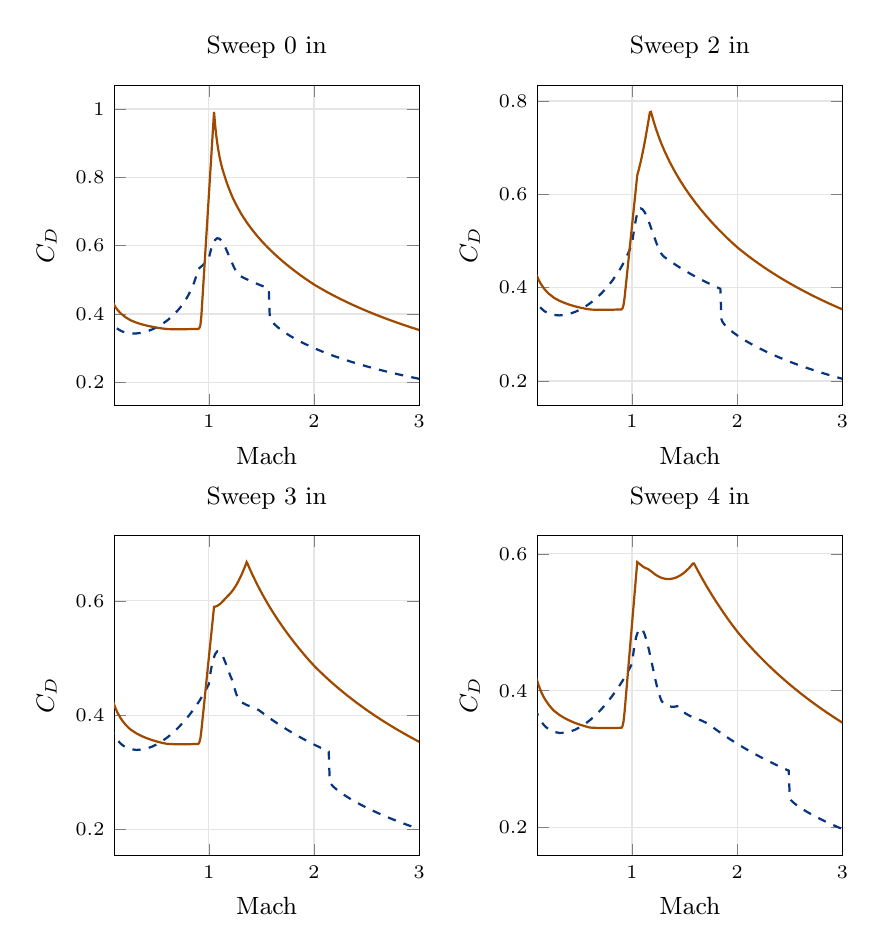
\begin{tikzpicture}
\begin{groupplot}[group style={group size=2 by 2,horizontal sep=1.50cm,vertical sep=1.65cm},width=.45\textwidth,height=5.65cm,grid=major,grid style={gray!20},tick label style={font=\scriptsize},label style={font=\small},title style={font=\small},scaled y ticks=false,yticklabel style={/pgf/number format/fixed,/pgf/number format/precision=3},unbounded coords=jump]
\nextgroupplot[title={Sweep 0 in},xlabel={Mach},ylabel={$C_D$},xmin=0.1,xmax=3]
\addplot[thick,B,dashed] coordinates {(0.01,0.4955666) (0.02,0.4463596) (0.03,0.4222005) (0.04,0.40681) (0.05,0.3957923) (0.06,0.3873641) (0.07,0.3806376) (0.08,0.3751113) (0.09,0.3704759) (0.11,0.3631295) (0.13,0.3576011) (0.16,0.3516121) (0.18,0.3487384) (0.21,0.3456879) (0.26,0.3431815) (0.31,0.3431771) (0.36,0.3452297) (0.41,0.3491168) (0.46,0.354744) (0.51,0.3621079) (0.56,0.3712875) (0.61,0.382456) (0.66,0.3959181) (0.71,0.4121886) (0.74,0.4236473) (0.76,0.4321655) (0.79,0.4465763) (0.81,0.4575376) (0.83,0.469888) (0.84,0.4767004) (0.86,0.4919286) (0.88,0.5099448) (0.89,0.5203522) (0.9,0.532136) (0.91,0.5344401) (0.94,0.5421597) (0.96,0.5480895) (1,0.5619391) (1.01,0.574947) (1.02,0.587778) (1.04,0.6057868) (1.06,0.6169265) (1.08,0.6217601) (1.1,0.6207864) (1.11,0.6176812) (1.12,0.6146123) (1.14,0.605021) (1.16,0.592891) (1.18,0.5791024) (1.21,0.5572927) (1.24,0.5365994) (1.26,0.5249949) (1.28,0.5161448) (1.3,0.5109336) (1.31,0.5093955) (1.36,0.5019799) (1.41,0.4949836) (1.46,0.4883551) (1.51,0.4820549) (1.56,0.4760491) (1.57,0.474881) (1.58,0.3886294) (1.59,0.3828108) (1.61,0.3748044) (1.63,0.3684281) (1.66,0.3602584) (1.71,0.348648) (1.76,0.3385303) (1.81,0.3294085) (1.86,0.3210334) (1.91,0.3132563) (1.96,0.3059777) (2.01,0.2991264) (2.06,0.2926488) (2.11,0.2865029) (2.16,0.2806546) (2.21,0.2750759) (2.26,0.2697432) (2.31,0.2646364) (2.36,0.2597381) (2.41,0.2550331) (2.46,0.2505079) (2.51,0.2461507) (2.56,0.2419508) (2.61,0.2378986) (2.66,0.2339856) (2.71,0.2302037) (2.76,0.2265459) (2.81,0.2230055) (2.86,0.2195766) (2.91,0.2162535) (2.96,0.2130311) (3,0.2105225)};
\addplot[thick,burntorange] coordinates {(0.01,0.6080662) (0.02,0.5395167) (0.03,0.5058317) (0.04,0.4843389) (0.05,0.4688985) (0.06,0.457018) (0.07,0.4474565) (0.08,0.4395131) (0.09,0.4327561) (0.11,0.4217564) (0.13,0.4130662) (0.16,0.4028202) (0.21,0.3902701) (0.26,0.3812657) (0.31,0.375082) (0.36,0.3701869) (0.41,0.3662012) (0.46,0.362888) (0.51,0.3600896) (0.56,0.3576965) (0.61,0.3559538) (0.66,0.3556905) (0.71,0.3556101) (0.76,0.3556828) (0.81,0.3558852) (0.86,0.3561986) (0.9,0.3565189) (0.91,0.3589432) (0.92,0.3662162) (0.93,0.3964753) (0.96,0.5453017) (1.01,0.7933456) (1.05,0.9917807) (1.06,0.9544623) (1.07,0.9251395) (1.08,0.9012349) (1.09,0.8812046) (1.1,0.8640597) (1.11,0.8491329) (1.12,0.835956) (1.13,0.8241895) (1.16,0.794207) (1.18,0.7766859) (1.21,0.7530062) (1.23,0.7388776) (1.26,0.7198364) (1.31,0.6923392) (1.36,0.6686089) (1.41,0.6475698) (1.46,0.6285588) (1.51,0.6111397) (1.56,0.5950108) (1.61,0.5799547) (1.66,0.5658094) (1.71,0.5524506) (1.76,0.5397811) (1.81,0.5277226) (1.86,0.5162118) (1.91,0.5051956) (1.96,0.4946296) (2.01,0.4846276) (2.06,0.475588) (2.11,0.4669043) (2.16,0.4585525) (2.21,0.4505112) (2.26,0.4427617) (2.31,0.4352867) (2.36,0.4280706) (2.41,0.4210989) (2.46,0.4143585) (2.51,0.4078372) (2.56,0.4015231) (2.61,0.3954055) (2.66,0.3894743) (2.71,0.3837197) (2.76,0.3781323) (2.81,0.3727032) (2.86,0.3674241) (2.91,0.3622866) (2.96,0.3572828) (3,0.3533708)};
\nextgroupplot[title={Sweep 2 in},xlabel={Mach},ylabel={$C_D$},xmin=0.1,xmax=3]
\addplot[thick,B,dashed] coordinates {(0.01,0.4955641) (0.02,0.4463494) (0.03,0.4221775) (0.04,0.4067691) (0.05,0.3957282) (0.06,0.3872718) (0.07,0.3805119) (0.08,0.3749468) (0.09,0.3702674) (0.11,0.3628168) (0.13,0.3571624) (0.16,0.350942) (0.18,0.3478849) (0.21,0.344513) (0.26,0.3413387) (0.31,0.3404814) (0.36,0.3414658) (0.41,0.3440277) (0.46,0.3480151) (0.51,0.3533434) (0.56,0.3599745) (0.61,0.3679075) (0.66,0.3771772) (0.71,0.3878581) (0.76,0.4000768) (0.81,0.414036) (0.86,0.4300604) (0.89,0.4408774) (0.91,0.4488272) (0.94,0.4620843) (0.96,0.4718286) (0.98,0.4824607) (1,0.4941793) (1.01,0.5092879) (1.02,0.5248091) (1.04,0.5493229) (1.05,0.5589202) (1.06,0.5673011) (1.08,0.5699125) (1.1,0.5679375) (1.11,0.5647763) (1.12,0.5617841) (1.14,0.5527196) (1.16,0.5415549) (1.21,0.5095672) (1.24,0.4911044) (1.26,0.4806203) (1.28,0.4723378) (1.3,0.4669846) (1.31,0.4653028) (1.36,0.4572011) (1.41,0.44957) (1.46,0.4423549) (1.51,0.4355126) (1.56,0.4290057) (1.61,0.4228036) (1.66,0.4168797) (1.71,0.4112111) (1.76,0.4057778) (1.81,0.4005626) (1.84,0.3975315) (1.85,0.3324413) (1.86,0.3266853) (1.88,0.3205237) (1.91,0.3135967) (1.96,0.3042054) (2.01,0.2961317) (2.06,0.2888585) (2.11,0.2821617) (2.16,0.2759171) (2.21,0.2700461) (2.26,0.264494) (2.31,0.2592207) (2.36,0.2541952) (2.41,0.2493927) (2.46,0.2447931) (2.51,0.2403793) (2.56,0.236137) (2.61,0.2320536) (2.66,0.2281182) (2.71,0.2243214) (2.76,0.2206544) (2.81,0.2171096) (2.86,0.2136802) (2.91,0.2103597) (2.96,0.2071425) (3,0.2046396)};
\addplot[thick,burntorange] coordinates {(0.01,0.6013536) (0.02,0.5338632) (0.03,0.5006926) (0.04,0.4795261) (0.05,0.4643194) (0.06,0.4526182) (0.07,0.4432008) (0.08,0.435377) (0.09,0.4287217) (0.11,0.4178874) (0.13,0.4093278) (0.16,0.3992357) (0.18,0.3937665) (0.21,0.3868742) (0.26,0.3780012) (0.31,0.3718913) (0.36,0.3670516) (0.41,0.3631086) (0.46,0.3598287) (0.51,0.3570564) (0.56,0.3546838) (0.61,0.3529459) (0.66,0.3526422) (0.71,0.3525196) (0.72,0.3525142) (0.76,0.3525489) (0.81,0.3527068) (0.86,0.3529746) (0.9,0.3532578) (0.91,0.35566) (0.92,0.3628665) (0.93,0.3791652) (0.96,0.4445285) (1.01,0.5534673) (1.05,0.6406183) (1.06,0.6487928) (1.08,0.6669688) (1.09,0.6769499) (1.11,0.6986613) (1.13,0.7226712) (1.16,0.7620479) (1.17,0.775677) (1.18,0.7766859) (1.21,0.7530062) (1.23,0.7388776) (1.26,0.7198364) (1.28,0.7082898) (1.31,0.6923392) (1.36,0.6686089) (1.41,0.6475698) (1.46,0.6285588) (1.51,0.6111397) (1.56,0.5950108) (1.61,0.5799547) (1.66,0.5658094) (1.71,0.5524506) (1.76,0.5397811) (1.81,0.5277226) (1.86,0.5162118) (1.91,0.5051956) (1.96,0.4946296) (2.01,0.4846276) (2.06,0.475588) (2.11,0.4669043) (2.16,0.4585525) (2.21,0.4505112) (2.26,0.4427617) (2.31,0.4352867) (2.36,0.4280706) (2.41,0.4210989) (2.46,0.4143585) (2.51,0.4078372) (2.56,0.4015231) (2.61,0.3954055) (2.66,0.3894743) (2.71,0.3837197) (2.76,0.3781323) (2.81,0.3727032) (2.86,0.3674241) (2.91,0.3622866) (2.96,0.3572828) (3,0.3533708)};
\nextgroupplot[title={Sweep 3 in},xlabel={Mach},ylabel={$C_D$},xmin=0.1,xmax=3]
\addplot[thick,B,dashed] coordinates {(0.01,0.4955628) (0.02,0.4463443) (0.03,0.4221661) (0.04,0.4067488) (0.05,0.3956966) (0.06,0.3872261) (0.07,0.3804497) (0.08,0.3748655) (0.09,0.3701644) (0.11,0.3626625) (0.13,0.3569461) (0.16,0.3506125) (0.18,0.3474659) (0.21,0.343938) (0.23,0.3422265) (0.26,0.3404426) (0.31,0.3391812) (0.36,0.3396686) (0.41,0.3416278) (0.46,0.3448898) (0.51,0.3493476) (0.56,0.3549334) (0.61,0.3616061) (0.66,0.369345) (0.71,0.3781464) (0.76,0.3880231) (0.81,0.3990055) (0.86,0.4111459) (0.91,0.4246619) (0.96,0.4402064) (1,0.4539038) (1.01,0.46628) (1.02,0.4787651) (1.04,0.496065) (1.06,0.5067121) (1.08,0.5116233) (1.1,0.5117255) (1.11,0.5095377) (1.12,0.5074911) (1.14,0.5003028) (1.16,0.4911436) (1.19,0.4759036) (1.21,0.4665336) (1.22,0.4623815) (1.23,0.457049) (1.24,0.4498603) (1.26,0.4376925) (1.28,0.4287398) (1.3,0.4238471) (1.31,0.4226102) (1.36,0.4177873) (1.41,0.4142287) (1.46,0.4102699) (1.48,0.4081432) (1.51,0.4041002) (1.56,0.3972551) (1.61,0.3907402) (1.66,0.3845266) (1.71,0.3785896) (1.76,0.3729073) (1.81,0.3674607) (1.86,0.3622327) (1.91,0.3572084) (1.96,0.352374) (2.01,0.3477177) (2.06,0.3432283) (2.11,0.338896) (2.14,0.3363682) (2.15,0.2825715) (2.16,0.2798042) (2.18,0.2756923) (2.21,0.2707168) (2.26,0.263726) (2.31,0.2575845) (2.36,0.2519762) (2.41,0.2467592) (2.46,0.2418537) (2.51,0.2372085) (2.56,0.2327878) (2.61,0.2285653) (2.66,0.2245203) (2.71,0.2206366) (2.76,0.2169005) (2.81,0.2133008) (2.86,0.2098276) (2.91,0.2064726) (2.96,0.2032283) (3,0.2007081)};
\addplot[thick,burntorange] coordinates {(0.01,0.5939472) (0.02,0.5276254) (0.03,0.4950223) (0.04,0.4742159) (0.05,0.4592669) (0.06,0.4477637) (0.07,0.4385053) (0.08,0.4308135) (0.09,0.4242704) (0.1,0.4186017) (0.11,0.4136185) (0.13,0.405203) (0.16,0.3952807) (0.18,0.3899036) (0.21,0.3831274) (0.24,0.377487) (0.26,0.3743993) (0.31,0.3683707) (0.36,0.3635922) (0.41,0.3596964) (0.46,0.3564532) (0.51,0.3537097) (0.56,0.3513596) (0.61,0.3496271) (0.66,0.3492788) (0.71,0.3491098) (0.74,0.3490821) (0.76,0.3490911) (0.81,0.3491998) (0.86,0.3494173) (0.9,0.3496598) (0.91,0.3520375) (0.92,0.3591706) (0.93,0.3735217) (0.96,0.4275295) (1.01,0.5175425) (1.05,0.5895529) (1.06,0.5897571) (1.08,0.591037) (1.11,0.5948037) (1.16,0.6044637) (1.21,0.6141389) (1.23,0.6187946) (1.26,0.6272225) (1.28,0.6337987) (1.31,0.6450956) (1.34,0.6581127) (1.36,0.6677494) (1.37,0.6642113) (1.41,0.6475698) (1.46,0.6285588) (1.51,0.6111397) (1.56,0.5950108) (1.61,0.5799547) (1.66,0.5658094) (1.71,0.5524506) (1.76,0.5397811) (1.81,0.5277226) (1.86,0.5162118) (1.91,0.5051956) (1.96,0.4946296) (2.01,0.4846276) (2.06,0.475588) (2.11,0.4669043) (2.16,0.4585525) (2.21,0.4505112) (2.26,0.4427617) (2.31,0.4352867) (2.36,0.4280706) (2.41,0.4210989) (2.46,0.4143585) (2.51,0.4078372) (2.56,0.4015231) (2.61,0.3954055) (2.66,0.3894743) (2.71,0.3837197) (2.76,0.3781323) (2.81,0.3727032) (2.86,0.3674241) (2.91,0.3622866) (2.96,0.3572828) (3,0.3533708)};
\nextgroupplot[title={Sweep 4 in},xlabel={Mach},ylabel={$C_D$},xmin=0.1,xmax=3]
\addplot[thick,B,dashed] coordinates {(0.01,0.4955621) (0.02,0.4463415) (0.03,0.4221597) (0.04,0.4067373) (0.05,0.3956786) (0.06,0.3872002) (0.07,0.3804143) (0.08,0.3748193) (0.09,0.3701059) (0.11,0.3625749) (0.13,0.3568235) (0.16,0.3504259) (0.18,0.3472289) (0.21,0.3436136) (0.23,0.3418356) (0.26,0.3399392) (0.31,0.3384548) (0.36,0.3386713) (0.41,0.3403069) (0.46,0.3431862) (0.51,0.3471947) (0.56,0.3522544) (0.61,0.3583117) (0.66,0.3653296) (0.71,0.3732834) (0.76,0.3821579) (0.81,0.3919458) (0.86,0.4026476) (0.91,0.4144078) (0.96,0.4277726) (1,0.4393144) (1.01,0.4510799) (1.02,0.4629209) (1.04,0.4788217) (1.06,0.4878998) (1.08,0.4910396) (1.1,0.4891272) (1.11,0.4858248) (1.12,0.4825817) (1.14,0.4727157) (1.16,0.4604176) (1.18,0.4465782) (1.21,0.4249381) (1.22,0.4178484) (1.24,0.404751) (1.26,0.3936996) (1.28,0.3856) (1.3,0.3813638) (1.31,0.3804075) (1.34,0.37809) (1.36,0.3770685) (1.39,0.3764987) (1.41,0.376916) (1.43,0.3775066) (1.46,0.3727592) (1.51,0.366726) (1.56,0.3625256) (1.61,0.3594235) (1.66,0.3565539) (1.71,0.3529445) (1.76,0.3476781) (1.81,0.342054) (1.86,0.3366609) (1.91,0.3314828) (1.96,0.3265051) (2.01,0.321715) (2.06,0.3171006) (2.11,0.3126512) (2.16,0.3083573) (2.21,0.3042101) (2.26,0.3002013) (2.31,0.2963238) (2.36,0.2925705) (2.41,0.2889353) (2.46,0.2854124) (2.49,0.2833503) (2.5,0.2430483) (2.51,0.240604) (2.53,0.2374095) (2.56,0.233615) (2.61,0.2282684) (2.66,0.2235344) (2.71,0.2191793) (2.76,0.2151014) (2.81,0.2112445) (2.86,0.2075729) (2.91,0.2040619) (2.96,0.2006932) (3,0.1980912)};
\addplot[thick,burntorange] coordinates {(0.01,0.5863164) (0.02,0.5211986) (0.03,0.4891801) (0.04,0.4687447) (0.05,0.4540613) (0.06,0.442762) (0.07,0.4336675) (0.08,0.4261116) (0.09,0.4196841) (0.1,0.4141154) (0.11,0.4092202) (0.13,0.4009531) (0.14,0.3974088) (0.16,0.3912058) (0.18,0.3859236) (0.21,0.3792669) (0.24,0.3737261) (0.26,0.3706882) (0.31,0.3647434) (0.36,0.3600281) (0.41,0.3561808) (0.46,0.3529754) (0.51,0.3502616) (0.56,0.3479347) (0.6,0.3463006) (0.61,0.3462077) (0.66,0.3458135) (0.71,0.3455966) (0.76,0.3455285) (0.81,0.3455865) (0.86,0.3457523) (0.9,0.3459527) (0.91,0.3483052) (0.92,0.3553626) (0.93,0.3697444) (0.96,0.4242766) (1.01,0.5151636) (1.05,0.5878732) (1.06,0.5866429) (1.11,0.5807182) (1.13,0.5790303) (1.15,0.5780496) (1.16,0.576851) (1.19,0.5736579) (1.21,0.5710699) (1.23,0.5688669) (1.26,0.5662524) (1.28,0.564955) (1.31,0.5636602) (1.33,0.5632242) (1.36,0.5632031) (1.38,0.5636076) (1.41,0.5648392) (1.43,0.5660756) (1.46,0.5685528) (1.49,0.5717779) (1.51,0.5743443) (1.54,0.5788208) (1.56,0.5822248) (1.58,0.5859661) (1.59,0.5858598) (1.61,0.5799547) (1.66,0.5658094) (1.71,0.5524506) (1.76,0.5397811) (1.81,0.5277226) (1.86,0.5162118) (1.91,0.5051956) (1.96,0.4946296) (2.01,0.4846276) (2.06,0.475588) (2.11,0.4669043) (2.16,0.4585525) (2.21,0.4505112) (2.26,0.4427617) (2.31,0.4352867) (2.36,0.4280706) (2.41,0.4210989) (2.46,0.4143585) (2.51,0.4078372) (2.56,0.4015231) (2.61,0.3954055) (2.66,0.3894743) (2.71,0.3837197) (2.76,0.3781323) (2.81,0.3727032) (2.86,0.3674241) (2.91,0.3622866) (2.96,0.3572828) (3,0.3533708)};
\end{groupplot}\end{tikzpicture}
\caption{Root/tip chords, span and thickness are fixed. Leading-edge sweep distance varies without fin overhang past the body.}\label{fig:atlas-10-Hbev-sweep}
\end{figure}
\noindent{\footnotesize Export files: \code{10-Hbev-sweep.svg} and \code{10-Hbev-sweep.png}.\\ Directory: \code{aerodynamic-investigation/extended/figures/}.}

\clearpage\subsubsection*{Fin span and aspect ratio}
\begin{figure}[H]\centering
{\footnotesize\begin{tabular}{ll}
\tikz[baseline=-.5ex]{\draw[thick,B,dashed] (0,0)--(.40,0);}\ MIT OR & \tikz[baseline=-.5ex]{\draw[thick,burntorange] (0,0)--(.40,0);}\ RASAero\\
\end{tabular}}\par\vspace{.7em}
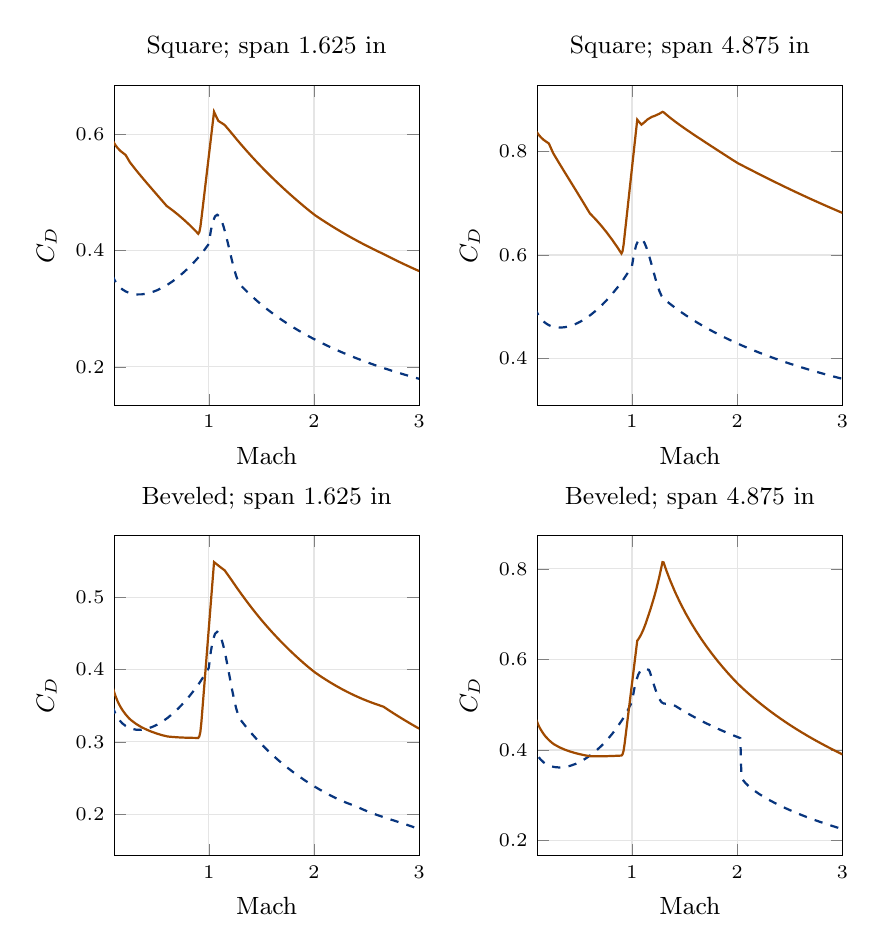
\begin{tikzpicture}
\begin{groupplot}[group style={group size=2 by 2,horizontal sep=1.50cm,vertical sep=1.65cm},width=.45\textwidth,height=5.65cm,grid=major,grid style={gray!20},tick label style={font=\scriptsize},label style={font=\small},title style={font=\small},scaled y ticks=false,yticklabel style={/pgf/number format/fixed,/pgf/number format/precision=3},unbounded coords=jump]
\nextgroupplot[title={Square; span 1.625 in},xlabel={Mach},ylabel={$C_D$},xmin=0.1,xmax=3]
\addplot[thick,B,dashed] coordinates {(0.01,0.4717587) (0.02,0.425809) (0.03,0.4032326) (0.04,0.3888323) (0.05,0.3785046) (0.06,0.3705848) (0.07,0.364244) (0.08,0.3590139) (0.09,0.3546059) (0.11,0.3475568) (0.13,0.3421652) (0.16,0.3361516) (0.18,0.3331347) (0.21,0.3297033) (0.26,0.3261583) (0.31,0.3246298) (0.36,0.3246594) (0.41,0.3259814) (0.46,0.3284292) (0.51,0.3318918) (0.56,0.3362921) (0.61,0.3415745) (0.66,0.3476977) (0.71,0.3546303) (0.76,0.3623482) (0.81,0.3708322) (0.86,0.3800671) (0.91,0.3901683) (0.96,0.4016204) (1,0.4114483) (1.01,0.4231358) (1.02,0.434838) (1.04,0.4504167) (1.06,0.4591101) (1.08,0.4617983) (1.1,0.4593625) (1.11,0.4557848) (1.12,0.4522472) (1.14,0.4417303) (1.16,0.428693) (1.18,0.4140174) (1.21,0.3909179) (1.22,0.3832808) (1.24,0.3689862) (1.26,0.3565856) (1.28,0.3469632) (1.3,0.3410033) (1.31,0.3390997) (1.36,0.3299436) (1.41,0.3213468) (1.46,0.3132497) (1.51,0.3056036) (1.56,0.2983652) (1.61,0.2914982) (1.66,0.28497) (1.71,0.2787527) (1.76,0.2728213) (1.81,0.2671539) (1.86,0.2617307) (1.91,0.2565344) (1.96,0.2515491) (2.01,0.2467608) (2.06,0.2421567) (2.11,0.2377253) (2.16,0.2334559) (2.21,0.2293391) (2.26,0.2253662) (2.31,0.221529) (2.36,0.2178203) (2.41,0.2142333) (2.46,0.2107617) (2.51,0.2073997) (2.56,0.204142) (2.61,0.2009836) (2.66,0.1979199) (2.71,0.1949466) (2.76,0.1920595) (2.81,0.1892551) (2.86,0.1865296) (2.91,0.1838798) (2.96,0.1813025) (3,0.179291)};
\addplot[thick,burntorange] coordinates {(0.01,0.6856544) (0.02,0.648) (0.03,0.6293194) (0.04,0.6173458) (0.05,0.6087206) (0.06,0.6020724) (0.07,0.5967153) (0.08,0.592261) (0.09,0.5884698) (0.11,0.5822944) (0.13,0.5774134) (0.16,0.5716578) (0.21,0.5646095) (0.25,0.5522528) (0.26,0.5498568) (0.31,0.538338) (0.36,0.5273447) (0.41,0.5166557) (0.46,0.5061327) (0.51,0.4956835) (0.56,0.4852434) (0.6,0.4768665) (0.61,0.4756019) (0.66,0.4688371) (0.71,0.4615702) (0.76,0.4537809) (0.81,0.4454528) (0.86,0.4365728) (0.9,0.4290641) (0.91,0.4319818) (0.92,0.4407347) (0.93,0.4549666) (0.96,0.50097) (1.01,0.5776424) (1.05,0.6389803) (1.06,0.6350937) (1.09,0.6236) (1.11,0.6211874) (1.15,0.6165241) (1.16,0.6144953) (1.21,0.6038027) (1.26,0.5927683) (1.31,0.582092) (1.36,0.5717468) (1.41,0.5617098) (1.46,0.5519608) (1.51,0.5425005) (1.56,0.533318) (1.61,0.5243916) (1.66,0.5157067) (1.71,0.5072507) (1.76,0.4990126) (1.81,0.4909822) (1.86,0.4831507) (1.91,0.4755092) (1.96,0.4680498) (2.01,0.4609797) (2.06,0.4549059) (2.11,0.4490038) (2.16,0.443269) (2.21,0.4376967) (2.26,0.432283) (2.31,0.4270235) (2.36,0.4219144) (2.41,0.4169515) (2.46,0.4121312) (2.51,0.4074498) (2.56,0.4029032) (2.61,0.3984881) (2.66,0.394173) (2.71,0.3895519) (2.76,0.3850392) (2.81,0.380631) (2.86,0.3763234) (2.91,0.3721124) (2.96,0.3679944) (3,0.3647644)};
\nextgroupplot[title={Square; span 4.875 in},xlabel={Mach},ylabel={$C_D$},xmin=0.1,xmax=3]
\addplot[thick,B,dashed] coordinates {(0.01,0.6256879) (0.02,0.5731991) (0.03,0.5474167) (0.04,0.5309789) (0.05,0.5191977) (0.06,0.5101713) (0.07,0.5029527) (0.08,0.4970069) (0.09,0.4920043) (0.1,0.4877281) (0.11,0.4840293) (0.13,0.4779636) (0.14,0.4754578) (0.16,0.4712641) (0.18,0.4679509) (0.21,0.464261) (0.23,0.4624895) (0.26,0.4606753) (0.31,0.4594955) (0.36,0.4601998) (0.41,0.4624868) (0.46,0.4661688) (0.51,0.471122) (0.56,0.4772615) (0.61,0.4845273) (0.66,0.4928763) (0.71,0.5022769) (0.76,0.512706) (0.81,0.5241468) (0.86,0.5365871) (0.91,0.5501644) (0.96,0.5654383) (1,0.5785329) (1.01,0.5909924) (1.02,0.6029306) (1.04,0.6190025) (1.06,0.6282107) (1.08,0.631429) (1.1,0.6295332) (1.11,0.6261977) (1.12,0.6229017) (1.14,0.6128652) (1.16,0.6003023) (1.18,0.5860927) (1.21,0.5636731) (1.22,0.5562569) (1.24,0.5423948) (1.26,0.5304135) (1.28,0.5211969) (1.3,0.515629) (1.31,0.5139161) (1.36,0.5056612) (1.41,0.4978791) (1.46,0.4905137) (1.51,0.4835211) (1.56,0.4768639) (1.61,0.4705111) (1.66,0.4644362) (1.71,0.4586164) (1.76,0.453032) (1.81,0.4476658) (1.86,0.4425023) (1.91,0.4375283) (1.96,0.4327316) (2.01,0.4281013) (2.06,0.4236277) (2.11,0.419302) (2.16,0.4151161) (2.21,0.4110626) (2.26,0.4071348) (2.31,0.4033266) (2.36,0.3996322) (2.41,0.3960462) (2.46,0.3925638) (2.51,0.3891804) (2.56,0.3858918) (2.61,0.3826939) (2.66,0.379583) (2.71,0.3765556) (2.76,0.3736084) (2.81,0.3707383) (2.86,0.3679423) (2.91,0.3652178) (2.96,0.362562) (3,0.3604852)};
\addplot[thick,burntorange] coordinates {(0.01,0.9366624) (0.02,0.8990079) (0.03,0.8803274) (0.04,0.8683537) (0.05,0.8597286) (0.06,0.8530803) (0.07,0.8477233) (0.08,0.843269) (0.09,0.8394777) (0.11,0.8333023) (0.13,0.8284214) (0.16,0.8226657) (0.21,0.8156175) (0.25,0.7973326) (0.26,0.7938628) (0.31,0.7768733) (0.36,0.7602402) (0.41,0.743742) (0.46,0.7272408) (0.51,0.7106438) (0.56,0.6938871) (0.6,0.6803347) (0.61,0.67837) (0.66,0.6677152) (0.71,0.6560939) (0.76,0.6434855) (0.81,0.6298739) (0.86,0.615246) (0.9,0.6028045) (0.91,0.6069036) (0.92,0.6192008) (0.96,0.6937317) (1.01,0.7870289) (1.05,0.8616667) (1.06,0.8590779) (1.09,0.8520847) (1.11,0.8552332) (1.15,0.862554) (1.16,0.8636868) (1.19,0.8672278) (1.21,0.8685325) (1.26,0.8731588) (1.29,0.8768422) (1.3,0.8761425) (1.31,0.8743518) (1.36,0.8658906) (1.41,0.858045) (1.46,0.8506173) (1.51,0.8434756) (1.56,0.8365299) (1.61,0.8297176) (1.66,0.8229951) (1.71,0.8163321) (1.76,0.8097085) (1.81,0.8031107) (1.86,0.7965308) (1.91,0.7899642) (1.96,0.7834089) (2.01,0.777126) (2.06,0.7718635) (2.11,0.7666292) (2.16,0.7614272) (2.21,0.7562616) (2.26,0.7511367) (2.31,0.7460562) (2.36,0.7410235) (2.41,0.7360411) (2.46,0.7311116) (2.51,0.7262367) (2.56,0.7214177) (2.61,0.7166553) (2.66,0.7119497) (2.71,0.7073008) (2.76,0.7027078) (2.81,0.6981694) (2.86,0.6936844) (2.91,0.6892505) (2.96,0.6848656) (3,0.6813911)};
\nextgroupplot[title={Beveled; span 1.625 in},xlabel={Mach},ylabel={$C_D$},xmin=0.1,xmax=3]
\addplot[thick,B,dashed] coordinates {(0.01,0.4639732) (0.02,0.4180231) (0.03,0.395446) (0.04,0.3810447) (0.05,0.3707158) (0.06,0.3627944) (0.07,0.3564518) (0.08,0.3512196) (0.09,0.3468092) (0.11,0.3397544) (0.13,0.334356) (0.16,0.3283302) (0.18,0.3253037) (0.21,0.3218557) (0.26,0.3182773) (0.31,0.3167081) (0.36,0.3166895) (0.41,0.3179559) (0.46,0.3203403) (0.51,0.3237316) (0.56,0.3280525) (0.61,0.3332471) (0.66,0.3392741) (0.71,0.3461018) (0.76,0.3537056) (0.81,0.3620663) (0.86,0.3711684) (0.91,0.3811269) (0.96,0.3924262) (1,0.4021243) (1.01,0.4137283) (1.02,0.4253938) (1.04,0.4408998) (1.06,0.4495219) (1.08,0.4521408) (1.1,0.4496379) (1.11,0.4460277) (1.12,0.4424582) (1.14,0.4318797) (1.16,0.418784) (1.18,0.404053) (1.21,0.3808766) (1.22,0.3732156) (1.24,0.3588757) (1.26,0.3464333) (1.28,0.3367724) (1.3,0.3307776) (1.31,0.3288578) (1.36,0.3196339) (1.41,0.3109909) (1.46,0.3028692) (1.51,0.2952199) (1.56,0.288) (1.61,0.2811734) (1.66,0.2747082) (1.71,0.2685775) (1.76,0.2627574) (1.81,0.2572278) (1.86,0.2519714) (1.91,0.2469736) (1.96,0.2422228) (2.01,0.2377099) (2.06,0.2334289) (2.11,0.2293773) (2.16,0.2255567) (2.21,0.2219743) (2.26,0.2186454) (2.31,0.2155975) (2.36,0.2128787) (2.41,0.2100618) (2.46,0.2067311) (2.51,0.2036829) (2.56,0.2008724) (2.61,0.1982538) (2.66,0.1957798) (2.71,0.1934026) (2.76,0.191073) (2.81,0.1887417) (2.86,0.1863584) (2.91,0.1838723) (2.96,0.1813025) (3,0.179291)};
\addplot[thick,burntorange] coordinates {(0.01,0.5226065) (0.02,0.4645823) (0.03,0.4360089) (0.04,0.4177591) (0.05,0.4046406) (0.06,0.3945426) (0.07,0.3864134) (0.08,0.3796587) (0.09,0.3739121) (0.1,0.3689331) (0.11,0.3645559) (0.13,0.3571635) (0.14,0.3539941) (0.16,0.3484472) (0.18,0.3437237) (0.21,0.3377715) (0.24,0.3328174) (0.26,0.3300729) (0.31,0.3246219) (0.36,0.3202783) (0.41,0.316717) (0.46,0.3137345) (0.51,0.3111954) (0.56,0.3090055) (0.61,0.3073108) (0.66,0.306646) (0.71,0.3061472) (0.76,0.3057879) (0.81,0.3055472) (0.86,0.3054081) (0.9,0.3053607) (0.91,0.3074372) (0.92,0.3136665) (0.93,0.3275453) (0.96,0.3827856) (1.01,0.4748528) (1.05,0.5485066) (1.06,0.5473171) (1.11,0.5415929) (1.15,0.537255) (1.16,0.5353094) (1.21,0.5250434) (1.26,0.5144507) (1.31,0.5042294) (1.36,0.4943508) (1.41,0.4847904) (1.46,0.4755949) (1.51,0.4668218) (1.56,0.4584022) (1.61,0.4503095) (1.66,0.4425254) (1.71,0.4350359) (1.76,0.4278292) (1.81,0.4208955) (1.86,0.4142262) (1.91,0.4078135) (1.96,0.4016505) (2.01,0.3958755) (2.06,0.3908937) (2.11,0.3861492) (2.16,0.3816384) (2.21,0.3773577) (2.26,0.3733042) (2.31,0.369475) (2.36,0.3658673) (2.41,0.3624783) (2.46,0.3593057) (2.51,0.3563469) (2.56,0.3535994) (2.61,0.351061) (2.66,0.348565) (2.71,0.3437393) (2.76,0.339045) (2.81,0.3344766) (2.86,0.3300289) (2.91,0.3256967) (2.96,0.3214749) (3,0.3181739)};
\nextgroupplot[title={Beveled; span 4.875 in},xlabel={Mach},ylabel={$C_D$},xmin=0.1,xmax=3]
\addplot[thick,B,dashed] coordinates {(0.01,0.5271523) (0.02,0.4746648) (0.03,0.4488845) (0.04,0.4324497) (0.05,0.4206724) (0.06,0.4116507) (0.07,0.4044377) (0.08,0.3984985) (0.09,0.3935033) (0.11,0.3855462) (0.13,0.3795023) (0.16,0.3728435) (0.18,0.3695633) (0.21,0.3659322) (0.26,0.3624735) (0.31,0.3614642) (0.36,0.3623932) (0.41,0.3649729) (0.46,0.3690335) (0.51,0.3744736) (0.56,0.3812376) (0.61,0.3893031) (0.66,0.3986758) (0.71,0.409389) (0.76,0.4215063) (0.81,0.4351297) (0.86,0.4504142) (0.91,0.467739) (0.96,0.4880291) (1,0.5064292) (1.01,0.5198153) (1.02,0.5333895) (1.04,0.553136) (1.06,0.5666527) (1.08,0.5749574) (1.1,0.5791163) (1.11,0.5792491) (1.12,0.5797686) (1.16,0.5770875) (1.17,0.572464) (1.21,0.5426165) (1.22,0.5355692) (1.24,0.5229383) (1.26,0.5127726) (1.28,0.5058445) (1.3,0.5029034) (1.31,0.5025823) (1.36,0.5011718) (1.39,0.4995419) (1.41,0.4976465) (1.46,0.4905137) (1.51,0.4835211) (1.56,0.4768639) (1.61,0.4705111) (1.66,0.4644362) (1.71,0.4586164) (1.76,0.453032) (1.81,0.4476658) (1.86,0.4425023) (1.91,0.4375283) (1.96,0.4327316) (2.01,0.4281013) (2.03,0.4262936) (2.04,0.3409545) (2.05,0.3357717) (2.06,0.3322805) (2.08,0.3267688) (2.11,0.3200727) (2.16,0.3108094) (2.21,0.3028192) (2.26,0.2956264) (2.31,0.2890111) (2.36,0.2828481) (2.41,0.2770574) (2.46,0.2715831) (2.51,0.2663842) (2.56,0.2614291) (2.61,0.2566931) (2.66,0.2521555) (2.71,0.2477995) (2.76,0.2436106) (2.81,0.2395766) (2.86,0.2356867) (2.91,0.2319314) (2.96,0.2283024) (3,0.225485)};
\addplot[thick,burntorange] coordinates {(0.01,0.6525945) (0.02,0.579978) (0.03,0.5443176) (0.04,0.5215717) (0.05,0.5052341) (0.06,0.4926648) (0.07,0.4825498) (0.08,0.474147) (0.09,0.4669997) (0.11,0.4553648) (0.13,0.4461732) (0.16,0.435336) (0.18,0.429463) (0.21,0.4220617) (0.24,0.4159006) (0.26,0.4125526) (0.31,0.4060858) (0.36,0.4009775) (0.41,0.3968279) (0.46,0.3933869) (0.51,0.3904883) (0.56,0.3880166) (0.61,0.3862554) (0.66,0.3861473) (0.71,0.3862285) (0.76,0.3864681) (0.81,0.3868419) (0.86,0.3873301) (0.9,0.3877924) (0.91,0.3904294) (0.92,0.3983404) (0.93,0.4137601) (0.96,0.4706795) (1.01,0.5655451) (1.05,0.6414376) (1.06,0.6444443) (1.08,0.6520332) (1.09,0.6565606) (1.11,0.6669913) (1.13,0.6791781) (1.16,0.6997236) (1.18,0.7142254) (1.21,0.7372269) (1.23,0.7542193) (1.26,0.782757) (1.29,0.8149511) (1.3,0.8144253) (1.31,0.8075526) (1.33,0.7944423) (1.36,0.776159) (1.41,0.7486733) (1.46,0.7241106) (1.51,0.7018247) (1.56,0.6813702) (1.61,0.6624274) (1.66,0.6447588) (1.71,0.6281828) (1.76,0.6125579) (1.81,0.5977709) (1.86,0.5837301) (1.91,0.5703592) (1.96,0.5575946) (2.01,0.5455437) (2.06,0.53462) (2.11,0.5241665) (2.16,0.5141488) (2.21,0.5045366) (2.26,0.4953029) (2.31,0.4864233) (2.36,0.4778758) (2.41,0.4696399) (2.46,0.4616971) (2.51,0.45403) (2.56,0.4466224) (2.61,0.4394593) (2.66,0.4325263) (2.71,0.42581) (2.76,0.4192974) (2.81,0.4129763) (2.86,0.4068349) (2.91,0.4008618) (2.96,0.3950463) (3,0.3905001)};
\end{groupplot}\end{tikzpicture}
\caption{Root/tip chords, sweep and thickness are fixed. Each solver uses the same exposed fin span.}\label{fig:atlas-11-fin-span}
\end{figure}
\noindent{\footnotesize Export files: \code{11-fin-span.svg} and \code{11-fin-span.png}.\\ Directory: \code{aerodynamic-investigation/extended/figures/}.}

\clearpage\subsubsection*{Fin taper at fixed sweep}
\begin{figure}[H]\centering
{\footnotesize\begin{tabular}{ll}
\tikz[baseline=-.5ex]{\draw[thick,B,dashed] (0,0)--(.40,0);}\ MIT OR & \tikz[baseline=-.5ex]{\draw[thick,burntorange] (0,0)--(.40,0);}\ RASAero\\
\end{tabular}}\par\vspace{.7em}
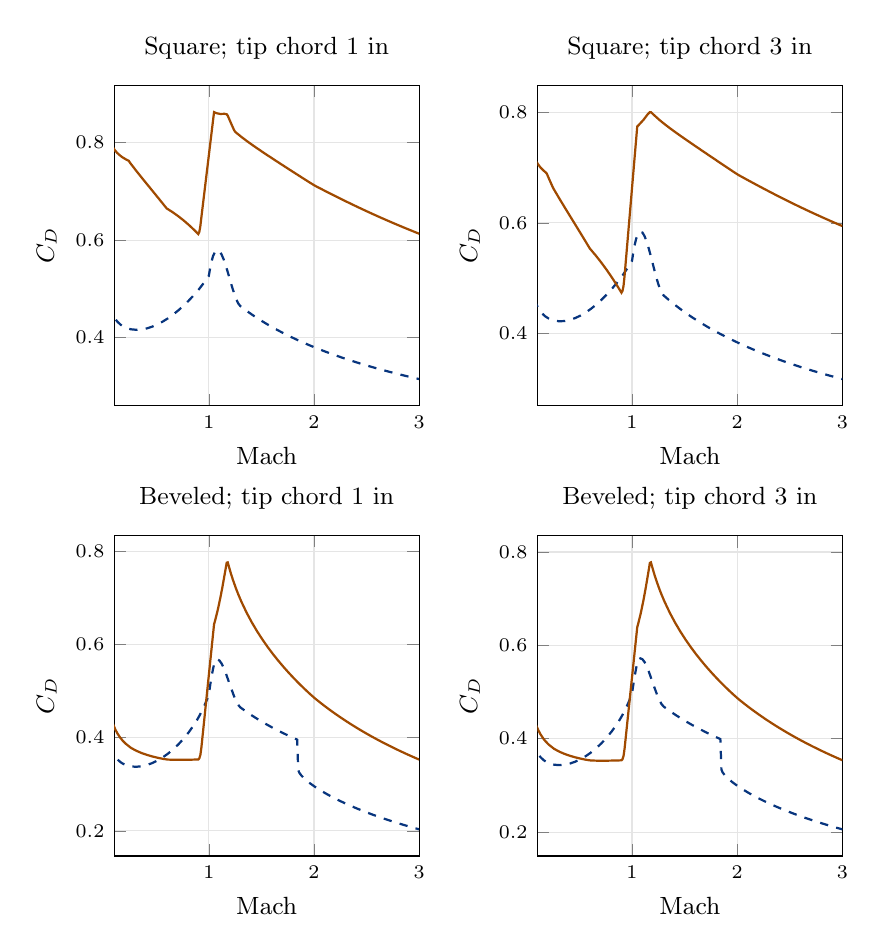
\begin{tikzpicture}
\begin{groupplot}[group style={group size=2 by 2,horizontal sep=1.50cm,vertical sep=1.65cm},width=.45\textwidth,height=5.65cm,grid=major,grid style={gray!20},tick label style={font=\scriptsize},label style={font=\small},title style={font=\small},scaled y ticks=false,yticklabel style={/pgf/number format/fixed,/pgf/number format/precision=3},unbounded coords=jump]
\nextgroupplot[title={Square; tip chord 1 in},xlabel={Mach},ylabel={$C_D$},xmin=0.1,xmax=3]
\addplot[thick,B,dashed] coordinates {(0.01,0.5694558) (0.02,0.5210402) (0.03,0.4972589) (0.04,0.4820973) (0.05,0.471231) (0.06,0.462906) (0.07,0.4562486) (0.08,0.4507655) (0.09,0.4461525) (0.1,0.4422098) (0.11,0.4387997) (0.13,0.4332088) (0.16,0.4270364) (0.18,0.423986) (0.21,0.4205921) (0.23,0.4189653) (0.26,0.4173038) (0.31,0.4162384) (0.36,0.4169143) (0.41,0.4190533) (0.46,0.4224819) (0.51,0.4270854) (0.56,0.4327853) (0.61,0.4395257) (0.66,0.4472664) (0.71,0.4559776) (0.76,0.4656376) (0.81,0.4762301) (0.86,0.4877433) (0.91,0.5003033) (0.96,0.5144256) (1,0.5265285) (1.01,0.5389381) (1.02,0.5509351) (1.04,0.5671132) (1.06,0.576414) (1.08,0.5797128) (1.1,0.5778868) (1.11,0.5746014) (1.12,0.5713541) (1.14,0.5614115) (1.16,0.5489383) (1.18,0.534815) (1.21,0.5125195) (1.22,0.5051436) (1.24,0.4913606) (1.26,0.4794569) (1.28,0.4703166) (1.3,0.464824) (1.31,0.4631485) (1.36,0.4550779) (1.41,0.4474774) (1.46,0.4402925) (1.51,0.4334798) (1.56,0.4270022) (1.61,0.420829) (1.66,0.4149334) (1.71,0.4092928) (1.76,0.4038871) (1.81,0.3986989) (1.86,0.3937128) (1.91,0.388915) (1.96,0.3842933) (2.01,0.3798368) (2.06,0.3755354) (2.11,0.3713803) (2.16,0.3673631) (2.21,0.3634765) (2.26,0.3597137) (2.31,0.3560683) (2.36,0.3525345) (2.41,0.3491071) (2.46,0.3457809) (2.51,0.3425516) (2.56,0.3394146) (2.61,0.3363662) (2.66,0.3334023) (2.71,0.3305197) (2.76,0.3277149) (2.81,0.324985) (2.86,0.3223268) (2.91,0.3197378) (2.96,0.3172152) (3,0.3152433)};
\addplot[thick,burntorange] coordinates {(0.01,0.8869449) (0.02,0.8492904) (0.03,0.8306099) (0.04,0.8186363) (0.05,0.8100111) (0.06,0.8033628) (0.07,0.7980058) (0.08,0.7935515) (0.09,0.7897602) (0.11,0.7835848) (0.13,0.7787039) (0.16,0.7729483) (0.18,0.7698294) (0.21,0.7659) (0.24,0.7626306) (0.25,0.7591033) (0.26,0.7562388) (0.31,0.7423189) (0.36,0.7288269) (0.41,0.7155417) (0.46,0.7023247) (0.51,0.6890838) (0.56,0.6757544) (0.6,0.6649959) (0.61,0.6637519) (0.66,0.6568168) (0.71,0.6491114) (0.76,0.6406156) (0.81,0.6313132) (0.86,0.6211907) (0.9,0.6124952) (0.91,0.6166601) (0.92,0.629155) (0.93,0.6474844) (0.96,0.7012337) (1.01,0.7908159) (1.05,0.8624816) (1.06,0.8614798) (1.08,0.8599361) (1.11,0.8587145) (1.15,0.8590245) (1.16,0.8585457) (1.17,0.8581697) (1.18,0.8552843) (1.21,0.8403712) (1.24,0.8258434) (1.25,0.8223244) (1.26,0.8204588) (1.31,0.8116633) (1.36,0.8035025) (1.41,0.7957493) (1.46,0.7882644) (1.51,0.7809585) (1.56,0.7737736) (1.61,0.7666718) (1.66,0.7596286) (1.71,0.7526284) (1.76,0.7456624) (1.81,0.7387258) (1.86,0.7318172) (1.91,0.7249365) (1.96,0.7180854) (2.01,0.7115134) (2.06,0.705931) (2.11,0.7003985) (2.16,0.6949205) (2.21,0.6895009) (2.26,0.6841438) (2.31,0.6788522) (2.36,0.673629) (2.41,0.6684762) (2.46,0.6633958) (2.51,0.6583888) (2.56,0.653456) (2.61,0.6485977) (2.66,0.6438138) (2.71,0.6391037) (2.76,0.6344666) (2.81,0.6299012) (2.86,0.6254061) (2.91,0.6209792) (2.96,0.6166186) (3,0.6131762)};
\nextgroupplot[title={Square; tip chord 3 in},xlabel={Mach},ylabel={$C_D$},xmin=0.1,xmax=3]
\addplot[thick,B,dashed] coordinates {(0.01,0.5810416) (0.02,0.5310335) (0.03,0.506468) (0.04,0.4908042) (0.05,0.479576) (0.06,0.4709713) (0.07,0.4640881) (0.08,0.4584166) (0.09,0.4536427) (0.1,0.44956) (0.11,0.4460264) (0.13,0.4402254) (0.16,0.4338024) (0.18,0.4306145) (0.21,0.4270449) (0.23,0.4253164) (0.26,0.4235197) (0.31,0.4222628) (0.36,0.4227768) (0.41,0.4247745) (0.46,0.4280763) (0.51,0.4325639) (0.56,0.4381559) (0.61,0.4447946) (0.66,0.4524383) (0.71,0.4610563) (0.76,0.4706258) (0.81,0.4811299) (0.86,0.4925563) (0.91,0.505035) (0.96,0.5190983) (1,0.5311596) (1.01,0.5435595) (1.02,0.5555473) (1.04,0.5717077) (1.06,0.5809924) (1.08,0.5842765) (1.1,0.5824374) (1.11,0.5791386) (1.12,0.575878) (1.14,0.5659089) (1.16,0.5534095) (1.18,0.53926) (1.21,0.5169257) (1.22,0.509537) (1.24,0.4957283) (1.26,0.4837993) (1.28,0.4746337) (1.3,0.4691161) (1.31,0.4674281) (1.36,0.4592957) (1.41,0.4516344) (1.46,0.4443896) (1.51,0.4375179) (1.56,0.4309821) (1.61,0.4247517) (1.66,0.4187997) (1.71,0.4131036) (1.76,0.4076431) (1.81,0.4024011) (1.86,0.3973619) (1.91,0.3925119) (1.96,0.3878388) (2.01,0.3833317) (2.06,0.3789805) (2.11,0.3747764) (2.16,0.3707111) (2.21,0.3667771) (2.26,0.3629677) (2.31,0.3592765) (2.36,0.3556977) (2.41,0.352226) (2.46,0.3488564) (2.51,0.3455843) (2.56,0.3424054) (2.61,0.3393157) (2.66,0.3363114) (2.71,0.333389) (2.76,0.3305451) (2.81,0.3277768) (2.86,0.325081) (2.91,0.3224549) (2.96,0.3198961) (3,0.3178956)};
\addplot[thick,burntorange] coordinates {(0.01,0.8083646) (0.02,0.7707101) (0.03,0.7520296) (0.04,0.7400559) (0.05,0.7314308) (0.06,0.7247825) (0.07,0.7194255) (0.08,0.7149712) (0.09,0.7111799) (0.11,0.7050045) (0.13,0.7001236) (0.16,0.694368) (0.18,0.6912491) (0.19,0.6891408) (0.21,0.6802234) (0.25,0.6632074) (0.26,0.6599135) (0.31,0.6438314) (0.36,0.6281534) (0.41,0.6126581) (0.46,0.597207) (0.51,0.5817081) (0.56,0.5660966) (0.6,0.553495) (0.61,0.5513727) (0.66,0.5400808) (0.71,0.5279528) (0.76,0.5149684) (0.81,0.5011115) (0.86,0.4863688) (0.9,0.4739295) (0.91,0.4771522) (0.92,0.4868204) (0.93,0.5052768) (0.96,0.5725087) (1.01,0.6845618) (1.05,0.7742042) (1.06,0.7759571) (1.11,0.7863028) (1.15,0.7963327) (1.16,0.798179) (1.17,0.8000864) (1.18,0.8000304) (1.21,0.794659) (1.26,0.7860999) (1.31,0.77835) (1.36,0.7710922) (1.41,0.7641442) (1.46,0.7573935) (1.51,0.7507685) (1.56,0.7442231) (1.61,0.7377281) (1.66,0.7312651) (1.71,0.7248232) (1.76,0.7183971) (1.81,0.711985) (1.86,0.7055875) (1.91,0.6992066) (1.96,0.6928453) (2.01,0.6867304) (2.06,0.6815048) (2.11,0.6763206) (2.16,0.6711831) (2.21,0.6660967) (2.26,0.6610656) (2.31,0.6560934) (2.36,0.6511832) (2.41,0.6463373) (2.46,0.6415577) (2.51,0.636846) (2.56,0.6322027) (2.61,0.6276287) (2.66,0.6231237) (2.71,0.6186875) (2.76,0.6143193) (2.81,0.6100178) (2.86,0.6057818) (2.91,0.6016094) (2.96,0.5974987) (3,0.5942529)};
\nextgroupplot[title={Beveled; tip chord 1 in},xlabel={Mach},ylabel={$C_D$},xmin=0.1,xmax=3]
\addplot[thick,B,dashed] coordinates {(0.01,0.4897318) (0.02,0.4413189) (0.03,0.4175418) (0.04,0.402386) (0.05,0.3915274) (0.06,0.3832117) (0.07,0.3765655) (0.08,0.3710953) (0.09,0.3664969) (0.11,0.3591789) (0.13,0.3536302) (0.16,0.347536) (0.18,0.3445481) (0.21,0.3412646) (0.26,0.3382097) (0.31,0.3374487) (0.36,0.3385146) (0.41,0.3411477) (0.46,0.345199) (0.51,0.3505856) (0.56,0.357271) (0.61,0.3652552) (0.66,0.3745736) (0.71,0.3853015) (0.76,0.3975658) (0.81,0.4115695) (0.86,0.4276376) (0.89,0.4384805) (0.91,0.4464453) (0.94,0.4597207) (0.96,0.4694764) (0.98,0.4801193) (1,0.4918481) (1.01,0.5069615) (1.02,0.5224874) (1.04,0.5470101) (1.05,0.5566115) (1.06,0.5649964) (1.08,0.5676152) (1.1,0.5656468) (1.11,0.5624923) (1.12,0.5595068) (1.14,0.5504557) (1.16,0.5393042) (1.21,0.5073492) (1.24,0.4889057) (1.26,0.4784343) (1.28,0.4701646) (1.3,0.464824) (1.31,0.4631485) (1.36,0.4550779) (1.41,0.4474774) (1.46,0.4402925) (1.51,0.4334798) (1.56,0.4270022) (1.61,0.420829) (1.66,0.4149334) (1.71,0.4092928) (1.76,0.4038871) (1.81,0.3986989) (1.84,0.3956839) (1.85,0.330599) (1.86,0.3248483) (1.88,0.3186973) (1.91,0.3117861) (1.96,0.3024206) (2.01,0.2943724) (2.06,0.2871243) (2.11,0.2804521) (2.16,0.2742318) (2.21,0.2683846) (2.26,0.262856) (2.31,0.2576057) (2.36,0.2526028) (2.41,0.2478227) (2.46,0.2432449) (2.51,0.2388526) (2.56,0.2346314) (2.61,0.2305688) (2.66,0.2266538) (2.71,0.222877) (2.76,0.2192297) (2.81,0.2157042) (2.86,0.2122937) (2.91,0.2089919) (2.96,0.205793) (3,0.2033044)};
\addplot[thick,burntorange] coordinates {(0.01,0.6030999) (0.02,0.5349758) (0.03,0.5015326) (0.04,0.480206) (0.05,0.4648909) (0.06,0.4531103) (0.07,0.4436315) (0.08,0.4357583) (0.09,0.4290623) (0.11,0.4181641) (0.13,0.4095562) (0.16,0.3994096) (0.18,0.393912) (0.21,0.3869852) (0.26,0.3780687) (0.31,0.3719266) (0.36,0.3670614) (0.41,0.3630974) (0.46,0.3597996) (0.51,0.3570118) (0.56,0.3546255) (0.61,0.3528752) (0.66,0.3525588) (0.71,0.3524243) (0.73,0.3524147) (0.76,0.3524422) (0.81,0.352589) (0.86,0.3528462) (0.9,0.3531211) (0.91,0.3555223) (0.92,0.362726) (0.93,0.3791189) (0.96,0.4450596) (1.01,0.554961) (1.05,0.642882) (1.06,0.6509766) (1.08,0.6688903) (1.09,0.6786925) (1.11,0.6999573) (1.13,0.7234082) (1.16,0.761747) (1.17,0.7749788) (1.18,0.7758158) (1.21,0.7521444) (1.23,0.7380214) (1.26,0.7189885) (1.28,0.7074474) (1.31,0.691505) (1.36,0.6677883) (1.41,0.6467627) (1.46,0.6277651) (1.51,0.6103592) (1.56,0.5942434) (1.61,0.5792004) (1.66,0.5650681) (1.71,0.5517222) (1.76,0.5390655) (1.81,0.5270198) (1.86,0.5155216) (1.91,0.504518) (1.96,0.4939645) (2.01,0.4839742) (2.06,0.4749435) (2.11,0.4662685) (2.16,0.4579254) (2.21,0.4498927) (2.26,0.4421516) (2.31,0.4346849) (2.36,0.4274771) (2.41,0.4205135) (2.46,0.4137812) (2.51,0.4072677) (2.56,0.4009614) (2.61,0.3948515) (2.66,0.3889278) (2.71,0.3831806) (2.76,0.3776006) (2.81,0.3721787) (2.86,0.3669067) (2.91,0.3617761) (2.96,0.3567792) (3,0.3528726)};
\nextgroupplot[title={Beveled; tip chord 3 in},xlabel={Mach},ylabel={$C_D$},xmin=0.1,xmax=3]
\addplot[thick,B,dashed] coordinates {(0.01,0.5013177) (0.02,0.4513121) (0.03,0.4267508) (0.04,0.411093) (0.05,0.3998724) (0.06,0.3912771) (0.07,0.384405) (0.08,0.3787464) (0.09,0.3739871) (0.11,0.3664056) (0.13,0.3606469) (0.16,0.3543021) (0.18,0.3511767) (0.21,0.3477175) (0.26,0.3444256) (0.31,0.3434732) (0.36,0.3443772) (0.41,0.3468689) (0.46,0.3507934) (0.51,0.3560641) (0.56,0.3626416) (0.61,0.3705241) (0.66,0.3797456) (0.71,0.3903802) (0.76,0.402554) (0.81,0.4164693) (0.86,0.4324506) (0.89,0.443242) (0.91,0.451177) (0.94,0.4644161) (0.96,0.4741492) (0.98,0.4847705) (1,0.4964792) (1.01,0.5115829) (1.02,0.5270995) (1.04,0.5516046) (1.05,0.5611978) (1.06,0.5695748) (1.08,0.5721789) (1.1,0.5701974) (1.11,0.5670296) (1.12,0.5640307) (1.14,0.5549531) (1.16,0.5437753) (1.21,0.5117554) (1.24,0.4932735) (1.26,0.4827767) (1.28,0.4744817) (1.3,0.4691161) (1.31,0.4674281) (1.36,0.4592957) (1.41,0.4516344) (1.46,0.4443896) (1.51,0.4375179) (1.56,0.4309821) (1.61,0.4247517) (1.66,0.4187997) (1.71,0.4131036) (1.76,0.4076431) (1.81,0.4024011) (1.84,0.3993541) (1.85,0.3342587) (1.86,0.3284975) (1.88,0.3223255) (1.91,0.315383) (1.96,0.3059661) (2.01,0.2978673) (2.06,0.2905694) (2.11,0.2838483) (2.16,0.2775798) (2.21,0.2716852) (2.26,0.26611) (2.31,0.260814) (2.36,0.2557661) (2.41,0.2509417) (2.46,0.2463204) (2.51,0.2418854) (2.56,0.2376222) (2.61,0.2335183) (2.66,0.2295629) (2.71,0.2257463) (2.76,0.2220599) (2.81,0.2184961) (2.86,0.2150479) (2.91,0.2117091) (2.96,0.2084739) (3,0.2059567)};
\addplot[thick,burntorange] coordinates {(0.01,0.6006897) (0.02,0.5336093) (0.03,0.5006083) (0.04,0.4795388) (0.05,0.4643962) (0.06,0.4527411) (0.07,0.4433587) (0.08,0.4355626) (0.09,0.4289298) (0.11,0.4181301) (0.13,0.409596) (0.16,0.3995318) (0.18,0.3940768) (0.21,0.3872015) (0.26,0.3783497) (0.31,0.3722585) (0.36,0.367434) (0.41,0.3635041) (0.46,0.3602356) (0.51,0.3574736) (0.56,0.3551103) (0.61,0.3533827) (0.66,0.353095) (0.71,0.3529881) (0.72,0.3529857) (0.76,0.3530328) (0.81,0.3532058) (0.86,0.3534887) (0.9,0.3537838) (0.91,0.3561895) (0.92,0.3634067) (0.93,0.3796265) (0.96,0.4444678) (1.01,0.5525367) (1.05,0.6389918) (1.06,0.6472239) (1.08,0.6656066) (1.09,0.6757333) (1.11,0.6978145) (1.13,0.7222929) (1.16,0.7625466) (1.17,0.7765128) (1.18,0.7776672) (1.21,0.7539775) (1.23,0.7398422) (1.26,0.7207913) (1.28,0.7092381) (1.31,0.6932777) (1.36,0.6695314) (1.41,0.6484764) (1.46,0.6294498) (1.51,0.6120151) (1.56,0.5958708) (1.61,0.5807996) (1.66,0.5666392) (1.71,0.5532655) (1.76,0.5405812) (1.81,0.528508) (1.86,0.5169827) (1.91,0.5059521) (1.96,0.4953717) (2.01,0.4853562) (2.06,0.4763064) (2.11,0.4676126) (2.16,0.4592508) (2.21,0.4511997) (2.26,0.4434405) (2.31,0.4359559) (2.36,0.4287305) (2.41,0.4217495) (2.46,0.415) (2.51,0.4084696) (2.56,0.4021467) (2.61,0.3960204) (2.66,0.3900806) (2.71,0.3843175) (2.76,0.3787218) (2.81,0.3732846) (2.86,0.3679975) (2.91,0.3628521) (2.96,0.3578405) (3,0.3539224)};
\end{groupplot}\end{tikzpicture}
\caption{Sweep is 2 in for all four cases; compare with the corresponding 2 in-sweep baseline, whose tip chord is 2 in.}\label{fig:atlas-12-tip-chord}
\end{figure}
\noindent{\footnotesize Export files: \code{12-tip-chord.svg} and \code{12-tip-chord.png}.\\ Directory: \code{aerodynamic-investigation/extended/figures/}.}

\clearpage\subsubsection*{Net drag added by fins}
\begin{figure}[H]\centering
{\footnotesize\begin{tabular}{ll}
\tikz[baseline=-.5ex]{\draw[thick,B,dashed] (0,0)--(.40,0);}\ MIT OR & \tikz[baseline=-.5ex]{\draw[thick,burntorange] (0,0)--(.40,0);}\ RASAero\\
\end{tabular}}\par\vspace{.7em}
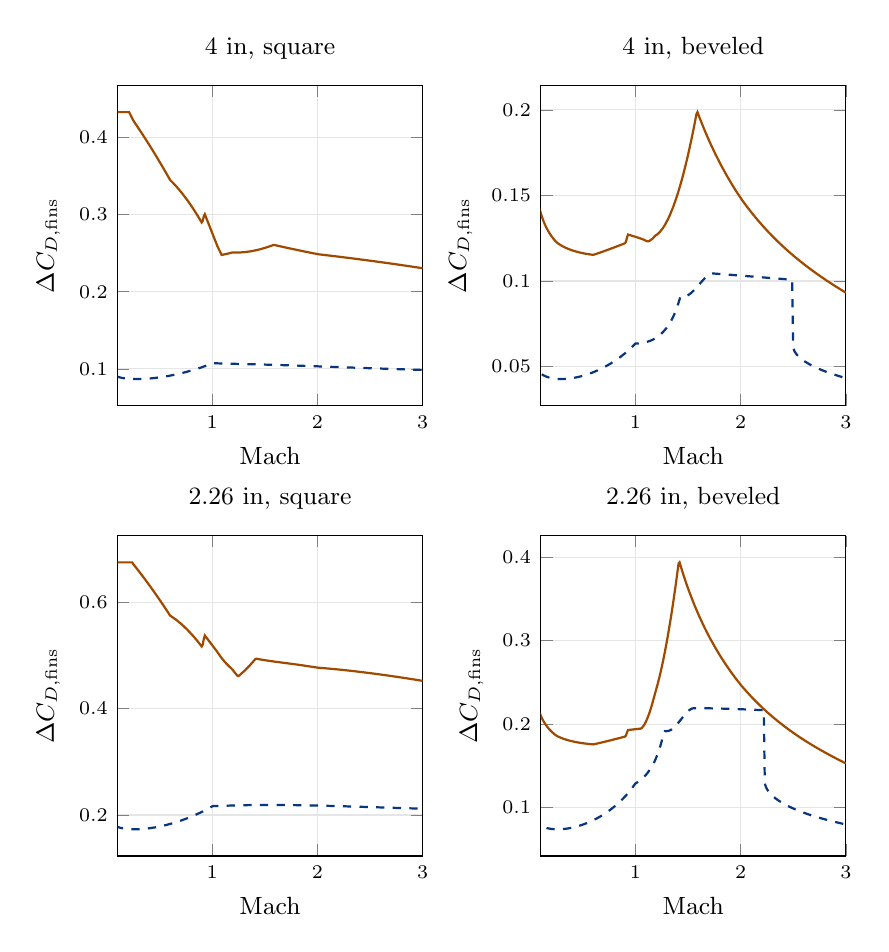
\begin{tikzpicture}
\begin{groupplot}[group style={group size=2 by 2,horizontal sep=1.50cm,vertical sep=1.65cm},width=.45\textwidth,height=5.65cm,grid=major,grid style={gray!20},tick label style={font=\scriptsize},label style={font=\small},title style={font=\small},scaled y ticks=false,yticklabel style={/pgf/number format/fixed,/pgf/number format/precision=3},unbounded coords=jump]
\nextgroupplot[title={4 in, square},xlabel={Mach},ylabel={$\Delta C_{D,\mathrm{fins}}$},xmin=0.1,xmax=3]
\addplot[thick,B,dashed] coordinates {(0.01,0.1068853) (0.02,0.1003426) (0.03,0.09713073) (0.04,0.095085) (0.05,0.09362091) (0.06,0.09250135) (0.07,0.09160826) (0.08,0.09087493) (0.09,0.09026025) (0.1,0.08973723) (0.11,0.08928726) (0.12,0.088897) (0.13,0.08855661) (0.14,0.0882586) (0.16,0.08776783) (0.18,0.0873912) (0.21,0.08699402) (0.23,0.08682059) (0.26,0.0866739) (0.28,0.0866422) (0.31,0.08668192) (0.33,0.08676146) (0.36,0.08695368) (0.38,0.08712744) (0.41,0.08745243) (0.43,0.08771012) (0.46,0.08815564) (0.48,0.08849075) (0.51,0.0890489) (0.53,0.08945719) (0.56,0.09012279) (0.58,0.09060144) (0.61,0.09137107) (0.66,0.09278976) (0.71,0.0943764) (0.76,0.09612974) (0.81,0.0980494) (0.86,0.1001357) (0.89,0.1014679) (0.91,0.1024078) (0.94,0.103902) (0.96,0.1049376) (1,0.1071052) (1.01,0.1072905) (1.06,0.1070153) (1.11,0.1068473) (1.16,0.1066319) (1.21,0.1064484) (1.26,0.1062793) (1.31,0.1061139) (1.36,0.1059459) (1.41,0.1057716) (1.46,0.1055892) (1.51,0.1053981) (1.56,0.1051984) (1.61,0.1049904) (1.66,0.1047749) (1.71,0.1045527) (1.76,0.1043248) (1.81,0.1040919) (1.86,0.103855) (1.91,0.1036149) (1.96,0.1033723) (2.01,0.1031278) (2.06,0.1028822) (2.11,0.1026359) (2.16,0.1023895) (2.21,0.1021435) (2.26,0.1018982) (2.31,0.101654) (2.36,0.1014111) (2.41,0.10117) (2.46,0.1009307) (2.51,0.1006936) (2.56,0.1004588) (2.61,0.1002264) (2.66,0.09999666) (2.71,0.09976957) (2.76,0.09954526) (2.81,0.09932382) (2.86,0.0991053) (2.91,0.09888975) (2.96,0.09867721) (3,0.09850936)};
\addplot[thick,burntorange] coordinates {(0.01,0.4332722) (0.04,0.4332722) (0.06,0.4332722) (0.11,0.4332722) (0.16,0.4332722) (0.21,0.4332722) (0.22,0.4307899) (0.25,0.4222829) (0.26,0.4202926) (0.31,0.4101517) (0.36,0.3996973) (0.41,0.3889292) (0.46,0.3778472) (0.51,0.3664517) (0.56,0.3547425) (0.6,0.3451492) (0.61,0.3438513) (0.66,0.3366405) (0.71,0.3285687) (0.76,0.3196359) (0.81,0.3098421) (0.86,0.2991874) (0.9,0.2900436) (0.91,0.2920159) (0.92,0.2979327) (0.93,0.3006364) (0.96,0.2902325) (1.01,0.2728926) (1.05,0.2590206) (1.06,0.2561949) (1.09,0.2478347) (1.11,0.2483546) (1.16,0.2499176) (1.19,0.2510356) (1.21,0.2509212) (1.26,0.2509833) (1.31,0.2514913) (1.36,0.2524038) (1.41,0.2536927) (1.46,0.2553375) (1.51,0.2573229) (1.56,0.2596379) (1.58,0.2606544) (1.59,0.2608206) (1.61,0.2601684) (1.66,0.2585993) (1.71,0.2570967) (1.76,0.255639) (1.81,0.2542095) (1.86,0.2527949) (1.91,0.2513849) (1.96,0.2499716) (2.01,0.2486797) (2.06,0.2478809) (2.11,0.2470728) (2.16,0.2462537) (2.21,0.2454226) (2.26,0.2445788) (2.31,0.2437221) (2.36,0.2428523) (2.41,0.2419695) (2.46,0.2410738) (2.51,0.2401653) (2.56,0.2392442) (2.61,0.2383102) (2.66,0.2373635) (2.71,0.2364037) (2.76,0.2354305) (2.81,0.2344434) (2.86,0.2334418) (2.91,0.2324248) (2.96,0.2313916) (3,0.2305527)};
\nextgroupplot[title={4 in, beveled},xlabel={Mach},ylabel={$\Delta C_{D,\mathrm{fins}}$},xmin=0.1,xmax=3]
\addplot[thick,B,dashed] coordinates {(0.01,0.06317714) (0.02,0.05663373) (0.03,0.05342065) (0.04,0.05137323) (0.05,0.04990699) (0.06,0.0487848) (0.07,0.0478886) (0.08,0.04715169) (0.09,0.04653297) (0.11,0.04555048) (0.13,0.04480849) (0.16,0.04399933) (0.18,0.0436069) (0.21,0.04318285) (0.26,0.04280993) (0.29,0.04274422) (0.31,0.04275611) (0.36,0.04295841) (0.41,0.04338188) (0.46,0.04400628) (0.51,0.04482008) (0.56,0.04581746) (0.61,0.04699669) (0.66,0.04835943) (0.71,0.04991033) (0.76,0.05165708) (0.81,0.05361071) (0.86,0.05578609) (0.91,0.05822113) (0.96,0.06101221) (1,0.06348128) (1.01,0.06347643) (1.06,0.0637301) (1.11,0.06445373) (1.14,0.06507583) (1.16,0.06560841) (1.19,0.06660438) (1.21,0.06741467) (1.24,0.06888208) (1.26,0.07005256) (1.29,0.07215048) (1.31,0.07381861) (1.33,0.07574544) (1.34,0.07682062) (1.36,0.07923184) (1.38,0.08205487) (1.39,0.08365104) (1.4,0.08539083) (1.41,0.0872933) (1.42,0.08938144) (1.43,0.09103184) (1.44,0.09089248) (1.46,0.09086906) (1.48,0.0911639) (1.49,0.09142118) (1.51,0.09213387) (1.53,0.09307875) (1.56,0.09483843) (1.61,0.09828335) (1.64,0.1003634) (1.66,0.1016342) (1.69,0.1032103) (1.71,0.1039457) (1.73,0.1043498) (1.74,0.1044058) (1.76,0.1043248) (1.81,0.1040919) (1.86,0.103855) (1.91,0.1036149) (1.96,0.1033723) (2.01,0.1031278) (2.06,0.1028822) (2.11,0.1026359) (2.16,0.1023895) (2.21,0.1021435) (2.26,0.1018982) (2.31,0.101654) (2.36,0.1014111) (2.41,0.10117) (2.46,0.1009307) (2.49,0.1007882) (2.5,0.06111785) (2.51,0.05930121) (2.52,0.05820899) (2.53,0.05735013) (2.54,0.05662014) (2.56,0.05539156) (2.58,0.05435671) (2.61,0.05302947) (2.66,0.05118961) (2.71,0.04964258) (2.76,0.04829054) (2.81,0.04708082) (2.86,0.04598114) (2.91,0.04497001) (2.96,0.04403222) (3,0.04332716)};
\addplot[thick,burntorange] coordinates {(0.01,0.2115638) (0.02,0.1841005) (0.03,0.1707626) (0.04,0.1623008) (0.05,0.1562426) (0.06,0.1515915) (0.07,0.1478541) (0.08,0.1447525) (0.09,0.1421162) (0.1,0.1398335) (0.11,0.1378277) (0.13,0.1344416) (0.14,0.1329901) (0.16,0.1304499) (0.18,0.1282865) (0.21,0.1255593) (0.24,0.1232879) (0.26,0.122152) (0.31,0.1202403) (0.36,0.118801) (0.41,0.1176938) (0.46,0.1168309) (0.51,0.1161544) (0.56,0.115624) (0.6,0.1152851) (0.61,0.1154989) (0.66,0.1165466) (0.71,0.1176381) (0.76,0.1187653) (0.81,0.1199217) (0.86,0.1211024) (0.9,0.1220616) (0.91,0.1228916) (0.92,0.1253817) (0.93,0.1271565) (0.96,0.1266001) (1.01,0.1256728) (1.06,0.124653) (1.11,0.1232897) (1.12,0.1231923) (1.13,0.1233407) (1.16,0.1245784) (1.19,0.126569) (1.21,0.1273703) (1.23,0.128506) (1.26,0.1308091) (1.28,0.1327322) (1.31,0.1361856) (1.33,0.1388624) (1.36,0.1434346) (1.39,0.148673) (1.41,0.1525351) (1.44,0.1588844) (1.46,0.1634893) (1.49,0.1709577) (1.51,0.1763129) (1.54,0.1849143) (1.56,0.1910305) (1.58,0.1974546) (1.59,0.198679) (1.61,0.1954141) (1.66,0.1877495) (1.71,0.1807077) (1.76,0.1741993) (1.81,0.1681538) (1.86,0.162514) (1.91,0.157233) (1.96,0.1522719) (2.01,0.1476465) (2.06,0.1434673) (2.11,0.139524) (2.16,0.135796) (2.21,0.132265) (2.26,0.1289148) (2.31,0.125731) (2.36,0.1227004) (2.41,0.119811) (2.46,0.1170521) (2.51,0.1144135) (2.56,0.1118859) (2.61,0.1094606) (2.66,0.1071295) (2.71,0.1048849) (2.76,0.1027195) (2.81,0.1006264) (2.86,0.09859907) (2.91,0.09663115) (2.96,0.0947166) (3,0.09321948)};
\nextgroupplot[title={2.26 in, square},xlabel={Mach},ylabel={$\Delta C_{D,\mathrm{fins}}$},xmin=0.1,xmax=3]
\addplot[thick,B,dashed] coordinates {(0.01,0.2065882) (0.02,0.1955157) (0.03,0.1901014) (0.04,0.1866627) (0.05,0.1842085) (0.06,0.1823373) (0.07,0.1808496) (0.08,0.1796326) (0.09,0.1786171) (0.1,0.1777574) (0.11,0.1770223) (0.13,0.1758418) (0.14,0.1753672) (0.16,0.1745999) (0.18,0.1740312) (0.21,0.1734728) (0.23,0.1732625) (0.26,0.1731508) (0.28,0.173196) (0.31,0.1734236) (0.33,0.1736734) (0.36,0.174184) (0.38,0.1746101) (0.41,0.1753709) (0.46,0.1769475) (0.51,0.1788904) (0.56,0.1811848) (0.61,0.1838214) (0.66,0.1867946) (0.71,0.1901016) (0.76,0.1937417) (0.81,0.1977157) (0.86,0.2020257) (0.89,0.2047742) (0.91,0.2067047) (0.94,0.2097583) (0.96,0.2118722) (1,0.216291) (1.01,0.2168855) (1.06,0.2170716) (1.11,0.2174335) (1.16,0.2176975) (1.21,0.217983) (1.26,0.2182561) (1.31,0.2184974) (1.36,0.2186967) (1.41,0.2188495) (1.46,0.2189548) (1.51,0.2190139) (1.55,0.2190295) (1.56,0.2190292) (1.61,0.2190038) (1.66,0.2189412) (1.71,0.2188449) (1.76,0.2187183) (1.81,0.2185646) (1.86,0.2183869) (1.91,0.2181881) (1.96,0.2179708) (2.01,0.2177373) (2.06,0.2174897) (2.11,0.2172301) (2.16,0.2169602) (2.21,0.2166815) (2.26,0.2163955) (2.31,0.2161035) (2.36,0.2158065) (2.41,0.2155056) (2.46,0.2152018) (2.51,0.2148958) (2.56,0.2145883) (2.61,0.21428) (2.66,0.2139715) (2.71,0.2136632) (2.76,0.2133556) (2.81,0.2130492) (2.86,0.2127442) (2.91,0.212441) (2.96,0.2121399) (3,0.2119006)};
\addplot[thick,burntorange] coordinates {(0.01,0.6747551) (0.02,0.6747551) (0.06,0.6747551) (0.11,0.6747551) (0.16,0.6747551) (0.21,0.6747551) (0.24,0.6747551) (0.25,0.6714917) (0.26,0.6690138) (0.31,0.6563719) (0.36,0.6433089) (0.41,0.6298249) (0.46,0.6159199) (0.51,0.601594) (0.56,0.586847) (0.6,0.5747463) (0.61,0.5735479) (0.66,0.5665237) (0.71,0.5583442) (0.76,0.5490093) (0.81,0.5385188) (0.86,0.526873) (0.9,0.5167245) (0.91,0.5202382) (0.92,0.5307794) (0.93,0.5373871) (0.96,0.5295984) (1.01,0.5166171) (1.05,0.5062322) (1.06,0.5032322) (1.08,0.4974745) (1.11,0.49002) (1.13,0.4855619) (1.16,0.4795123) (1.19,0.4738938) (1.21,0.4687909) (1.24,0.4617185) (1.25,0.4611105) (1.26,0.4627235) (1.31,0.4715752) (1.36,0.4816964) (1.41,0.4930501) (1.42,0.4938186) (1.46,0.4922796) (1.51,0.490631) (1.56,0.4891798) (1.61,0.4878414) (1.66,0.4865552) (1.71,0.4852774) (1.76,0.4839765) (1.81,0.4826304) (1.86,0.4812238) (1.91,0.4797466) (1.96,0.4781926) (2.01,0.4767531) (2.06,0.4759859) (2.11,0.4751506) (2.16,0.4742498) (2.21,0.4732871) (2.26,0.4722661) (2.31,0.4711905) (2.36,0.470064) (2.41,0.4688901) (2.46,0.4676717) (2.51,0.4664117) (2.56,0.4651125) (2.61,0.463776) (2.66,0.4624036) (2.71,0.4609964) (2.76,0.4595551) (2.81,0.4580798) (2.86,0.4565703) (2.91,0.455026) (2.96,0.4534459) (3,0.4521551)};
\nextgroupplot[title={2.26 in, beveled},xlabel={Mach},ylabel={$\Delta C_{D,\mathrm{fins}}$},xmin=0.1,xmax=3]
\addplot[thick,B,dashed] coordinates {(0.01,0.1072643) (0.02,0.09619168) (0.03,0.09077713) (0.04,0.08733818) (0.05,0.08488356) (0.06,0.0830119) (0.08,0.08030604) (0.09,0.07928985) (0.11,0.07769373) (0.13,0.07651183) (0.16,0.07526823) (0.21,0.07414061) (0.26,0.07382454) (0.31,0.07411488) (0.36,0.07491087) (0.41,0.07616005) (0.46,0.07783623) (0.51,0.07992973) (0.56,0.08244288) (0.61,0.08538805) (0.66,0.08878733) (0.71,0.09267337) (0.76,0.09709134) (0.81,0.1021023) (0.86,0.1077886) (0.91,0.1142922) (0.96,0.1218838) (1,0.1288158) (1.01,0.1294983) (1.04,0.1319575) (1.06,0.1339739) (1.08,0.1363309) (1.11,0.1405502) (1.14,0.1457077) (1.16,0.1498461) (1.18,0.1546667) (1.19,0.1573754) (1.21,0.1634996) (1.22,0.1669708) (1.23,0.1707602) (1.24,0.1749104) (1.25,0.1794725) (1.26,0.1845089) (1.27,0.1900968) (1.28,0.1916446) (1.29,0.1914448) (1.31,0.1916295) (1.33,0.1925476) (1.34,0.1932599) (1.36,0.1951373) (1.38,0.1975342) (1.41,0.2018478) (1.46,0.2097949) (1.49,0.2141389) (1.51,0.2164865) (1.53,0.2181698) (1.54,0.2186991) (1.56,0.2190292) (1.61,0.2190038) (1.66,0.2189412) (1.71,0.2188449) (1.76,0.2187183) (1.81,0.2185646) (1.86,0.2183869) (1.91,0.2181881) (1.96,0.2179708) (2.01,0.2177373) (2.06,0.2174897) (2.11,0.2172301) (2.16,0.2169602) (2.21,0.2166815) (2.22,0.2166249) (2.23,0.1289988) (2.24,0.1247871) (2.25,0.1222238) (2.26,0.1202105) (2.28,0.1169982) (2.31,0.1132394) (2.33,0.1111408) (2.36,0.1083838) (2.41,0.1044896) (2.46,0.1011808) (2.51,0.09827797) (2.56,0.09567822) (2.61,0.09331627) (2.66,0.09114744) (2.71,0.08913961) (2.76,0.0872687) (2.81,0.0855161) (2.86,0.08386711) (2.91,0.08230982) (2.96,0.08083443) (3,0.07970757)};
\addplot[thick,burntorange] coordinates {(0.01,0.3115339) (0.02,0.2726163) (0.03,0.2537606) (0.04,0.2418145) (0.05,0.2332698) (0.06,0.2267145) (0.07,0.2214499) (0.08,0.2170831) (0.09,0.2133729) (0.11,0.2073407) (0.13,0.2025804) (0.16,0.196972) (0.18,0.1939338) (0.21,0.1901053) (0.24,0.186918) (0.26,0.1853219) (0.31,0.1826283) (0.36,0.1805985) (0.41,0.1790351) (0.46,0.177815) (0.51,0.1768565) (0.56,0.176103) (0.6,0.1756201) (0.61,0.1759134) (0.66,0.1773512) (0.71,0.1788505) (0.76,0.1804) (0.81,0.1819905) (0.86,0.1836152) (0.9,0.1849356) (0.91,0.1861932) (0.92,0.1899658) (0.93,0.192865) (0.96,0.1932831) (1.01,0.1939799) (1.05,0.1945374) (1.06,0.1952191) (1.08,0.1982649) (1.09,0.200405) (1.11,0.2057119) (1.13,0.2122523) (1.14,0.215953) (1.16,0.224174) (1.19,0.2382113) (1.21,0.2471221) (1.23,0.2570638) (1.24,0.2624175) (1.26,0.2738858) (1.28,0.2863648) (1.3,0.2998524) (1.31,0.3069743) (1.33,0.3219754) (1.34,0.3298552) (1.36,0.3463755) (1.38,0.363914) (1.39,0.3730667) (1.41,0.3921429) (1.42,0.3937758) (1.46,0.3774223) (1.48,0.3698603) (1.51,0.359181) (1.56,0.3429089) (1.61,0.3282348) (1.66,0.3148853) (1.71,0.302653) (1.76,0.2913771) (1.81,0.2809302) (1.86,0.2712096) (1.91,0.2621311) (1.96,0.2536244) (2.01,0.2456952) (2.06,0.2384767) (2.11,0.2316788) (2.16,0.225264) (2.21,0.2191995) (2.26,0.213456) (2.31,0.2080073) (2.36,0.2028299) (2.41,0.1979022) (2.46,0.1932048) (2.51,0.1887193) (2.56,0.1844291) (2.61,0.1803185) (2.66,0.1763729) (2.71,0.1725785) (2.76,0.1689221) (2.81,0.1653915) (2.86,0.1619747) (2.91,0.1586606) (2.96,0.1554381) (3,0.1529192)};
\end{groupplot}\end{tikzpicture}
\caption{Finned-minus-finless subtraction includes fin/body interference and changes in exposed body surface. It is not an isolated RASAero fin-pressure coefficient.}\label{fig:atlas-13-fin-increments}
\end{figure}
\noindent{\footnotesize Export files: \code{13-fin-increments.svg} and \code{13-fin-increments.png}.\\ Directory: \code{aerodynamic-investigation/extended/figures/}.}

\clearpage\subsubsection*{Thin-profile limits and rounded control}
\begin{figure}[H]\centering
{\footnotesize\begin{tabular}{ll}
\tikz[baseline=-.5ex]{\draw[thick,B,dashed] (0,0)--(.40,0);}\ MIT OR & \tikz[baseline=-.5ex]{\draw[thick,burntorange] (0,0)--(.40,0);}\ RASAero\\
\end{tabular}}\par\vspace{.7em}
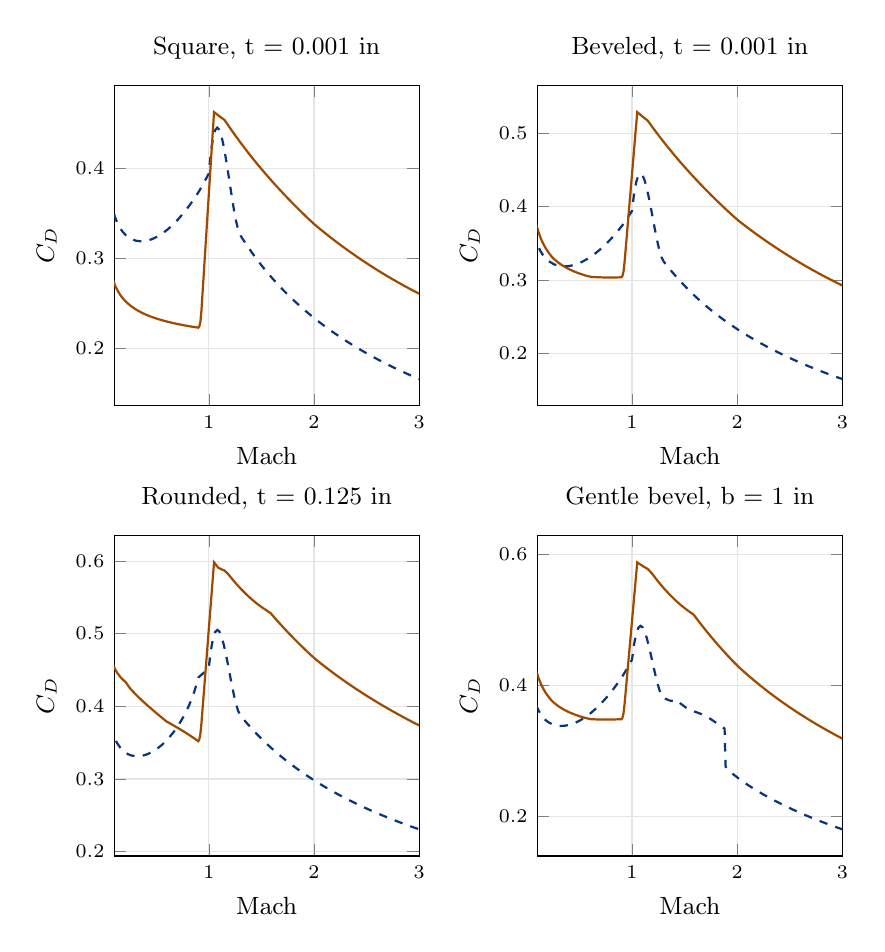
\begin{tikzpicture}
\begin{groupplot}[group style={group size=2 by 2,horizontal sep=1.50cm,vertical sep=1.65cm},width=.45\textwidth,height=5.65cm,grid=major,grid style={gray!20},tick label style={font=\scriptsize},label style={font=\small},title style={font=\small},scaled y ticks=false,yticklabel style={/pgf/number format/fixed,/pgf/number format/precision=3},unbounded coords=jump]
\nextgroupplot[title={Square, t = 0.001 in},xlabel={Mach},ylabel={$C_D$},xmin=0.1,xmax=3]
\addplot[thick,B,dashed] coordinates {(0.01,0.4779451) (0.02,0.4290703) (0.03,0.4050499) (0.04,0.3897213) (0.05,0.3787203) (0.06,0.3702764) (0.07,0.3635079) (0.08,0.357917) (0.09,0.3531965) (0.11,0.3456234) (0.13,0.3397977) (0.16,0.3332363) (0.18,0.3298981) (0.21,0.3260256) (0.26,0.3218072) (0.31,0.3196378) (0.36,0.3190297) (0.41,0.3197002) (0.46,0.3214717) (0.51,0.324226) (0.56,0.3278808) (0.61,0.3323765) (0.66,0.3376691) (0.71,0.3437247) (0.76,0.3505172) (0.81,0.3580258) (0.86,0.3662339) (0.91,0.3752637) (0.96,0.3856301) (1,0.3945593) (1.01,0.4062939) (1.02,0.4180853) (1.04,0.4338353) (1.06,0.442692) (1.08,0.4455365) (1.1,0.443251) (1.11,0.4397331) (1.12,0.4362533) (1.14,0.4258472) (1.16,0.4129145) (1.18,0.3983376) (1.21,0.3753767) (1.22,0.3677834) (1.24,0.3535731) (1.26,0.3412527) (1.28,0.3317065) (1.3,0.3258195) (1.31,0.3239509) (1.36,0.3149589) (1.41,0.3065089) (1.46,0.2985438) (1.51,0.2910166) (1.56,0.2838857) (1.61,0.2771161) (1.66,0.2706763) (1.71,0.2645393) (1.76,0.2586809) (1.81,0.2530799) (1.86,0.2477171) (1.91,0.2425757) (1.96,0.2376404) (2.01,0.2328976) (2.06,0.2283347) (2.11,0.2239408) (2.16,0.2197054) (2.21,0.2156194) (2.26,0.2116743) (2.31,0.2078623) (2.36,0.2041762) (2.41,0.2006096) (2.46,0.1971562) (2.51,0.1938105) (2.56,0.1905674) (2.61,0.1874219) (2.66,0.1843696) (2.71,0.1814062) (2.76,0.1785278) (2.81,0.1757309) (2.86,0.1730118) (2.91,0.1703675) (2.96,0.1677947) (3,0.1657862)};
\addplot[thick,burntorange] coordinates {(0.01,0.3731641) (0.02,0.3355096) (0.03,0.3168291) (0.04,0.3048554) (0.05,0.2962303) (0.06,0.289582) (0.07,0.2842249) (0.08,0.2797707) (0.09,0.2759794) (0.11,0.269804) (0.13,0.2649231) (0.16,0.2591674) (0.18,0.2560486) (0.21,0.2521192) (0.26,0.2470096) (0.31,0.243025) (0.36,0.2397988) (0.41,0.2371101) (0.46,0.2348205) (0.51,0.2328375) (0.56,0.231097) (0.61,0.229547) (0.66,0.2281395) (0.71,0.2268697) (0.76,0.225717) (0.81,0.2246652) (0.86,0.2237012) (0.9,0.222986) (0.91,0.2245023) (0.92,0.2290512) (0.93,0.2416782) (0.96,0.2969697) (1.01,0.3891222) (1.05,0.4628442) (1.06,0.4619137) (1.11,0.4574325) (1.15,0.454029) (1.16,0.4523137) (1.21,0.4437686) (1.26,0.4355297) (1.31,0.4275792) (1.36,0.4198921) (1.41,0.4124473) (1.46,0.4052268) (1.51,0.3982149) (1.56,0.3913981) (1.61,0.3847647) (1.66,0.378304) (1.71,0.372007) (1.76,0.3658654) (1.81,0.3598719) (1.86,0.35402) (1.91,0.3483036) (1.96,0.3427171) (2.01,0.3373579) (2.06,0.3325123) (2.11,0.3277862) (2.16,0.3231763) (2.21,0.3186795) (2.26,0.3142932) (2.31,0.3100148) (2.36,0.3058416) (2.41,0.3017712) (2.46,0.2978013) (2.51,0.2939297) (2.56,0.2901539) (2.61,0.2864721) (2.66,0.282882) (2.71,0.2793816) (2.76,0.2759689) (2.81,0.2726418) (2.86,0.2693986) (2.91,0.2662371) (2.96,0.2631555) (3,0.2607466)};
\nextgroupplot[title={Beveled, t = 0.001 in},xlabel={Mach},ylabel={$C_D$},xmin=0.1,xmax=3]
\addplot[thick,B,dashed] coordinates {(0.01,0.4775954) (0.02,0.4287206) (0.03,0.4047002) (0.04,0.3893716) (0.05,0.3783706) (0.06,0.3699266) (0.07,0.3631582) (0.08,0.3575672) (0.09,0.3528467) (0.11,0.3452735) (0.13,0.3394477) (0.16,0.3328861) (0.18,0.3295478) (0.21,0.3256752) (0.26,0.3214563) (0.31,0.3192864) (0.36,0.3186778) (0.41,0.3193476) (0.46,0.3211185) (0.51,0.3238722) (0.56,0.3275263) (0.61,0.3320215) (0.66,0.3373137) (0.71,0.343369) (0.76,0.3501614) (0.81,0.3576703) (0.86,0.3658791) (0.91,0.3749102) (0.96,0.3852787) (1,0.3942103) (1.01,0.4059434) (1.02,0.4177354) (1.04,0.4334871) (1.06,0.4423457) (1.08,0.4451927) (1.1,0.4429102) (1.11,0.4393939) (1.12,0.435916) (1.14,0.4255141) (1.16,0.4125863) (1.18,0.3980151) (1.21,0.3750644) (1.22,0.367475) (1.24,0.3532734) (1.26,0.3409629) (1.28,0.3314281) (1.3,0.3255539) (1.31,0.3236926) (1.36,0.3147452) (1.41,0.3063611) (1.46,0.2984102) (1.51,0.2908201) (1.56,0.2835977) (1.61,0.2767271) (1.66,0.270196) (1.71,0.2639966) (1.76,0.2581203) (1.81,0.2525149) (1.86,0.2471481) (1.91,0.2420031) (1.96,0.2370644) (2.01,0.2323184) (2.06,0.2277526) (2.11,0.2233559) (2.16,0.219118) (2.21,0.2150296) (2.26,0.2110822) (2.31,0.2072681) (2.36,0.2035801) (2.41,0.2000116) (2.46,0.1965565) (2.51,0.1932092) (2.56,0.1899645) (2.61,0.1868175) (2.66,0.1837638) (2.71,0.1807991) (2.76,0.1779195) (2.81,0.1751213) (2.86,0.1724011) (2.91,0.1697557) (2.96,0.167182) (3,0.1651726)};
\addplot[thick,burntorange] coordinates {(0.01,0.5389437) (0.02,0.4754307) (0.03,0.4441918) (0.04,0.4242508) (0.05,0.4099215) (0.06,0.3988939) (0.07,0.3900178) (0.08,0.3826432) (0.09,0.3763697) (0.1,0.3709345) (0.11,0.3661565) (0.13,0.3580873) (0.14,0.3546278) (0.16,0.3485732) (0.18,0.3434174) (0.21,0.3369201) (0.24,0.331512) (0.26,0.3285405) (0.31,0.3227074) (0.36,0.3180762) (0.41,0.3142936) (0.46,0.3111386) (0.51,0.3084644) (0.56,0.3061685) (0.61,0.3044488) (0.66,0.3039933) (0.71,0.3037127) (0.76,0.3035787) (0.81,0.3035691) (0.86,0.3036659) (0.9,0.3038103) (0.91,0.3058762) (0.92,0.3120739) (0.93,0.3252079) (0.96,0.3761222) (1.01,0.4609792) (1.05,0.5288649) (1.06,0.5276345) (1.11,0.5217098) (1.15,0.5172161) (1.16,0.5152321) (1.21,0.5053654) (1.26,0.4958393) (1.31,0.4866333) (1.36,0.47772) (1.41,0.4690763) (1.46,0.4606824) (1.51,0.4525208) (1.56,0.4445768) (1.61,0.4368365) (1.66,0.429288) (1.71,0.4219218) (1.76,0.4147286) (1.81,0.4077001) (1.86,0.400829) (1.91,0.3941084) (1.96,0.3875319) (2.01,0.3812455) (2.06,0.3756751) (2.11,0.3702377) (2.16,0.36493) (2.21,0.3597486) (2.26,0.3546908) (2.31,0.3497536) (2.36,0.3449346) (2.41,0.3402307) (2.46,0.3356397) (2.51,0.3311592) (2.56,0.3267865) (2.61,0.3225195) (2.66,0.3183557) (2.71,0.3142932) (2.76,0.3103294) (2.81,0.3064624) (2.86,0.3026899) (2.91,0.2990098) (2.96,0.29542) (3,0.2926119)};
\nextgroupplot[title={Rounded, t = 0.125 in},xlabel={Mach},ylabel={$C_D$},xmin=0.1,xmax=3]
\addplot[thick,B,dashed] coordinates {(0.01,0.4878037) (0.02,0.4385845) (0.03,0.4144049) (0.04,0.3989857) (0.05,0.3879311) (0.06,0.3794578) (0.07,0.3726779) (0.08,0.3670899) (0.09,0.3623844) (0.11,0.3548726) (0.13,0.3491446) (0.16,0.3427912) (0.18,0.3396301) (0.21,0.3360796) (0.23,0.334353) (0.26,0.3325476) (0.31,0.3312587) (0.36,0.3317401) (0.41,0.3337318) (0.46,0.3370885) (0.51,0.3417371) (0.56,0.3476591) (0.61,0.3548874) (0.66,0.363516) (0.71,0.3737295) (0.76,0.3858688) (0.79,0.3943283) (0.81,0.4005931) (0.84,0.4112008) (0.86,0.419333) (0.88,0.4286412) (0.89,0.4338769) (0.9,0.4396765) (0.91,0.4408726) (0.96,0.4474003) (1,0.453289) (1.01,0.4651485) (1.02,0.4770658) (1.04,0.493064) (1.06,0.502163) (1.08,0.5052436) (1.1,0.5031876) (1.11,0.4997802) (1.12,0.4964091) (1.14,0.4862149) (1.16,0.4734866) (1.18,0.4591068) (1.21,0.4364276) (1.22,0.4289246) (1.24,0.4148895) (1.26,0.4027373) (1.28,0.3933526) (1.3,0.3876203) (1.31,0.3858267) (1.36,0.3771863) (1.41,0.3690517) (1.46,0.3613688) (1.51,0.3540941) (1.56,0.3471887) (1.61,0.3406202) (1.66,0.3343598) (1.71,0.3283825) (1.76,0.3226662) (1.81,0.3171914) (1.86,0.3119407) (1.91,0.3068986) (1.96,0.3020511) (2.01,0.2973858) (2.06,0.2928911) (2.11,0.288557) (2.16,0.2843739) (2.21,0.2803334) (2.26,0.2764276) (2.31,0.2726494) (2.36,0.2689921) (2.41,0.2654497) (2.46,0.2620166) (2.51,0.2586874) (2.56,0.2554574) (2.61,0.252322) (2.66,0.249277) (2.71,0.2463185) (2.76,0.2434428) (2.81,0.2406464) (2.86,0.2379261) (2.91,0.2352788) (2.96,0.2327016) (3,0.2306885)};
\addplot[thick,burntorange] coordinates {(0.01,0.554368) (0.02,0.5167136) (0.03,0.498033) (0.04,0.4860594) (0.05,0.4774342) (0.06,0.470786) (0.07,0.4654289) (0.08,0.4609746) (0.09,0.4571834) (0.11,0.4510079) (0.13,0.446127) (0.16,0.4403714) (0.18,0.4372525) (0.21,0.4333231) (0.25,0.4251324) (0.26,0.4234909) (0.31,0.4158165) (0.36,0.4087864) (0.41,0.4021798) (0.46,0.3958579) (0.51,0.3897286) (0.56,0.3837276) (0.6,0.3789875) (0.61,0.3782149) (0.66,0.3741837) (0.71,0.3699769) (0.76,0.3655739) (0.81,0.3609587) (0.86,0.3561179) (0.9,0.3520757) (0.91,0.3544698) (0.92,0.3616521) (0.93,0.3762873) (0.96,0.4317779) (1.01,0.5242623) (1.05,0.5982497) (1.06,0.5963754) (1.09,0.5908795) (1.11,0.5894698) (1.15,0.5869077) (1.16,0.5854805) (1.19,0.581165) (1.21,0.5774913) (1.26,0.5688664) (1.31,0.560975) (1.36,0.5537616) (1.41,0.5471864) (1.46,0.5412197) (1.51,0.5358377) (1.56,0.5310222) (1.59,0.5280377) (1.61,0.5246526) (1.66,0.516407) (1.71,0.5084454) (1.76,0.5007401) (1.81,0.4932681) (1.86,0.4860105) (1.91,0.4789507) (1.96,0.4720746) (2.01,0.4655202) (2.06,0.4597047) (2.11,0.4540472) (2.16,0.4485407) (2.21,0.4431783) (2.26,0.4379543) (2.31,0.4328632) (2.36,0.4279001) (2.41,0.4230597) (2.46,0.4183376) (2.51,0.4137295) (2.56,0.4092306) (2.61,0.404837) (2.66,0.4005442) (2.71,0.3963483) (2.76,0.3922448) (2.81,0.3882297) (2.86,0.3842988) (2.91,0.3804479) (2.96,0.3766726) (3,0.3737042)};
\nextgroupplot[title={Gentle bevel, b = 1 in},xlabel={Mach},ylabel={$C_D$},xmin=0.1,xmax=3]
\addplot[thick,B,dashed] coordinates {(0.01,0.4955621) (0.02,0.4463415) (0.03,0.4221597) (0.04,0.4067373) (0.05,0.3956786) (0.06,0.3872002) (0.07,0.3804143) (0.08,0.3748193) (0.09,0.3701059) (0.11,0.3625749) (0.13,0.3568235) (0.16,0.3504259) (0.18,0.3472289) (0.21,0.3436136) (0.26,0.3399392) (0.31,0.3384548) (0.36,0.3386713) (0.41,0.3403069) (0.46,0.3431862) (0.51,0.3471947) (0.56,0.3522544) (0.61,0.3583117) (0.66,0.3653296) (0.71,0.3732834) (0.76,0.3821579) (0.81,0.3919458) (0.86,0.4026476) (0.91,0.4144078) (0.96,0.4277726) (1,0.4393144) (1.01,0.4510799) (1.02,0.4629209) (1.04,0.4788217) (1.06,0.4878998) (1.08,0.4910396) (1.1,0.4891272) (1.11,0.4858248) (1.12,0.4825817) (1.14,0.4727157) (1.16,0.4604176) (1.18,0.4465782) (1.21,0.4249381) (1.22,0.4178484) (1.24,0.404751) (1.26,0.3936996) (1.28,0.3856) (1.3,0.3813638) (1.31,0.3804075) (1.36,0.3770685) (1.39,0.3764987) (1.41,0.376916) (1.43,0.3775066) (1.46,0.3727592) (1.51,0.366726) (1.56,0.3625256) (1.61,0.3594235) (1.66,0.3565539) (1.71,0.3529445) (1.76,0.3476781) (1.81,0.342054) (1.86,0.3366609) (1.88,0.3345647) (1.89,0.2762771) (1.91,0.2724443) (1.96,0.2650805) (2.01,0.2587603) (2.06,0.2529753) (2.11,0.2475652) (2.16,0.2424515) (2.21,0.2375876) (2.26,0.2329419) (2.31,0.2284911) (2.36,0.2242172) (2.41,0.2201057) (2.46,0.2161444) (2.51,0.2123229) (2.56,0.2086322) (2.61,0.2050643) (2.66,0.2016122) (2.71,0.1982694) (2.76,0.1950302) (2.81,0.1918893) (2.86,0.1888419) (2.91,0.1858835) (2.96,0.18301) (3,0.1807698)};
\addplot[thick,burntorange] coordinates {(0.01,0.5920161) (0.02,0.525999) (0.03,0.4935439) (0.04,0.4728313) (0.05,0.4579496) (0.06,0.4464979) (0.07,0.437281) (0.08,0.4296236) (0.09,0.4231097) (0.1,0.4174664) (0.11,0.4125055) (0.13,0.4041275) (0.14,0.4005357) (0.16,0.3942495) (0.18,0.3888964) (0.21,0.3821504) (0.24,0.3765352) (0.26,0.3734602) (0.31,0.3674528) (0.36,0.3626903) (0.41,0.3588067) (0.46,0.3555731) (0.51,0.3528371) (0.56,0.3504929) (0.61,0.3487618) (0.66,0.3484019) (0.71,0.3482208) (0.76,0.3481895) (0.81,0.3482854) (0.86,0.3484899) (0.9,0.3487217) (0.91,0.351093) (0.92,0.3582069) (0.93,0.3725156) (0.96,0.426355) (1.01,0.5160873) (1.05,0.5878732) (1.06,0.5866914) (1.11,0.5814496) (1.15,0.5778407) (1.16,0.5761177) (1.19,0.5708856) (1.21,0.5665926) (1.26,0.5564306) (1.31,0.5470513) (1.36,0.5384235) (1.41,0.5305243) (1.46,0.5233363) (1.51,0.5168462) (1.56,0.5110441) (1.58,0.5089142) (1.59,0.5074033) (1.61,0.5030912) (1.66,0.4926125) (1.71,0.4825322) (1.76,0.4728167) (1.81,0.4634376) (1.86,0.4543713) (1.91,0.4455968) (1.96,0.4370958) (2.01,0.4290037) (2.06,0.4217373) (2.11,0.4147051) (2.16,0.4078963) (2.21,0.4013005) (2.26,0.3949085) (2.31,0.3887114) (2.36,0.3827009) (2.41,0.3768687) (2.46,0.3712076) (2.51,0.3657099) (2.56,0.3603685) (2.61,0.3551766) (2.66,0.3501274) (2.71,0.3452144) (2.76,0.3404311) (2.81,0.3357712) (2.86,0.3312286) (2.91,0.3267971) (2.96,0.3224707) (3,0.3190814)};
\end{groupplot}\end{tikzpicture}
\caption{These limits test whether the models approach a consistent finite-planform, vanishing-thickness behavior.}\label{fig:atlas-14-profile-limits}
\end{figure}
\noindent{\footnotesize Export files: \code{14-profile-limits.svg} and \code{14-profile-limits.png}.\\ Directory: \code{aerodynamic-investigation/extended/figures/}.}

\clearpage\subsubsection*{Geometric scale and Reynolds number}
\begin{figure}[H]\centering
{\footnotesize\begin{tabular}{ll}
\tikz[baseline=-.5ex]{\draw[thick,B,dashed] (0,0)--(.40,0);}\ MIT OR & \tikz[baseline=-.5ex]{\draw[thick,burntorange] (0,0)--(.40,0);}\ RASAero\\
\end{tabular}}\par\vspace{.7em}
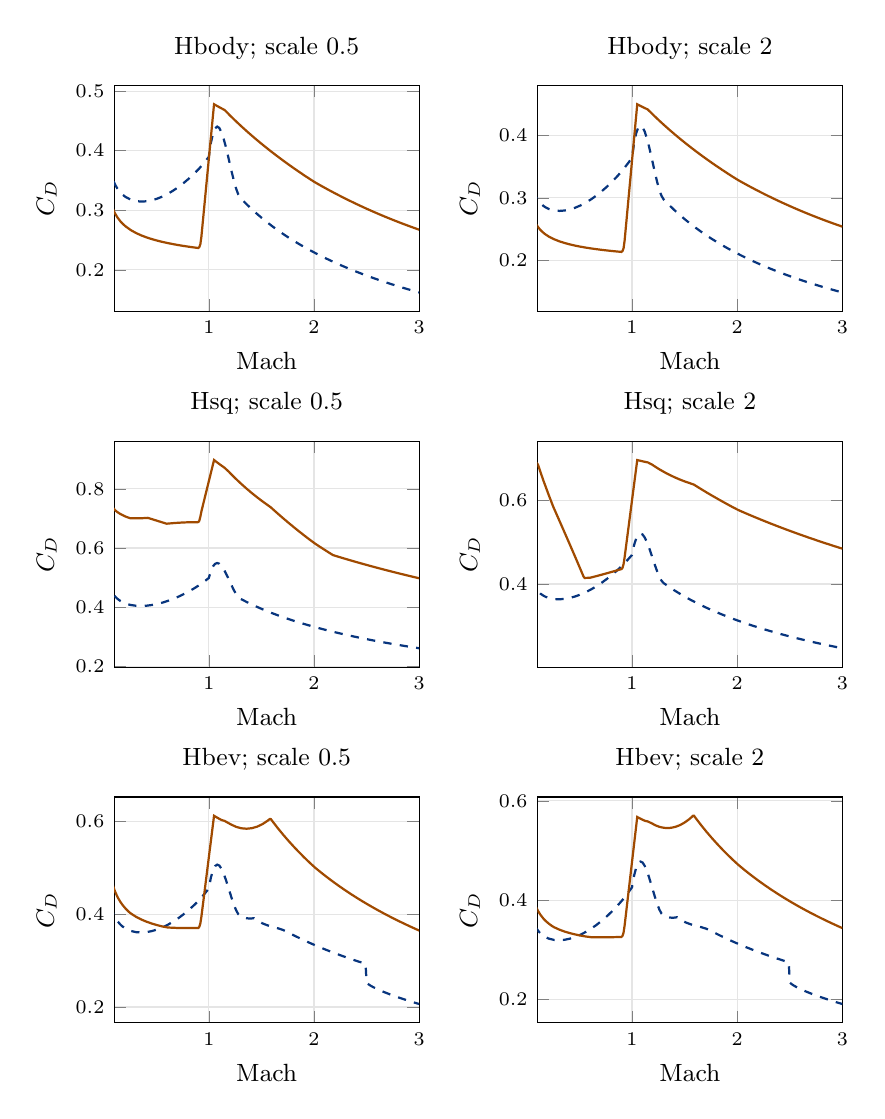
\begin{tikzpicture}
\begin{groupplot}[group style={group size=2 by 3,horizontal sep=1.50cm,vertical sep=1.65cm},width=.45\textwidth,height=4.45cm,grid=major,grid style={gray!20},tick label style={font=\scriptsize},label style={font=\small},title style={font=\small},scaled y ticks=false,yticklabel style={/pgf/number format/fixed,/pgf/number format/precision=3},unbounded coords=jump]
\nextgroupplot[title={Hbody; scale 0.5},xlabel={Mach},ylabel={$C_D$},xmin=0.1,xmax=3]
\addplot[thick,B,dashed] coordinates {(0.01,0.4861768) (0.02,0.4324143) (0.03,0.406344) (0.04,0.3898313) (0.05,0.3780401) (0.06,0.3690231) (0.07,0.3618158) (0.08,0.3558757) (0.09,0.3508693) (0.11,0.3428529) (0.13,0.3366969) (0.16,0.3297691) (0.18,0.3262431) (0.21,0.3221453) (0.26,0.31765) (0.31,0.3152817) (0.36,0.3145241) (0.41,0.3150789) (0.46,0.3167591) (0.51,0.3194407) (0.56,0.3230371) (0.61,0.327486) (0.66,0.3327413) (0.71,0.3387675) (0.76,0.3455375) (0.81,0.3530296) (0.86,0.3612262) (0.91,0.3702452) (0.96,0.3805846) (1,0.3894896) (1.01,0.4012208) (1.02,0.4130106) (1.04,0.4287569) (1.06,0.4376089) (1.08,0.4404478) (1.1,0.4381556) (1.11,0.4346411) (1.12,0.4311648) (1.14,0.4207659) (1.16,0.4078408) (1.18,0.3932719) (1.21,0.3703234) (1.22,0.3627345) (1.24,0.3485331) (1.26,0.3362219) (1.28,0.3266853) (1.3,0.320808) (1.31,0.3189445) (1.36,0.3099786) (1.41,0.3015562) (1.46,0.2936202) (1.51,0.2861234) (1.56,0.2790241) (1.61,0.272287) (1.66,0.2658807) (1.71,0.259778) (1.76,0.2539545) (1.81,0.248389) (1.86,0.2430622) (1.91,0.2379573) (1.96,0.2330588) (2.01,0.2283529) (2.06,0.2238273) (2.11,0.2194707) (2.16,0.2152727) (2.21,0.2112242) (2.26,0.2073165) (2.31,0.2035418) (2.36,0.199893) (2.41,0.1963635) (2.46,0.192947) (2.51,0.1896381) (2.56,0.1864315) (2.61,0.1833223) (2.66,0.1803059) (2.71,0.1773783) (2.76,0.1745353) (2.81,0.1717734) (2.86,0.1690891) (2.91,0.1664791) (2.96,0.1639404) (3,0.1619589)};
\addplot[thick,burntorange] coordinates {(0.01,0.4213159) (0.02,0.3747526) (0.03,0.3517797) (0.04,0.3370981) (0.05,0.3265426) (0.06,0.3184175) (0.07,0.3118774) (0.08,0.3064439) (0.09,0.3018222) (0.1,0.2978187) (0.11,0.2943) (0.13,0.2883595) (0.16,0.2813592) (0.18,0.2775679) (0.21,0.2727931) (0.26,0.2665116) (0.31,0.2616144) (0.36,0.2576371) (0.41,0.2543108) (0.46,0.251467) (0.51,0.2489937) (0.56,0.2468127) (0.61,0.2448677) (0.66,0.2431167) (0.71,0.2415277) (0.76,0.2400758) (0.81,0.2387413) (0.86,0.2375083) (0.9,0.2365861) (0.91,0.2381949) (0.92,0.2430213) (0.93,0.2558931) (0.96,0.3114055) (1.01,0.4039261) (1.05,0.4779426) (1.06,0.4769217) (1.11,0.4720248) (1.15,0.4683315) (1.16,0.4665448) (1.21,0.4576581) (1.26,0.4490977) (1.31,0.4408336) (1.36,0.4328401) (1.41,0.4250958) (1.46,0.4175822) (1.51,0.4102834) (1.56,0.4031855) (1.61,0.3962766) (1.66,0.3895459) (1.71,0.3829838) (1.76,0.376582) (1.81,0.3703327) (1.86,0.3642295) (1.91,0.3582659) (1.96,0.3524362) (2.01,0.3468491) (2.06,0.3418235) (2.11,0.336921) (2.16,0.3321385) (2.21,0.3274727) (2.26,0.3229209) (2.31,0.3184804) (2.36,0.3141486) (2.41,0.3099229) (2.46,0.305801) (2.51,0.3017807) (2.56,0.2978594) (2.61,0.2940352) (2.66,0.2903058) (2.71,0.2866692) (2.76,0.2831232) (2.81,0.2796658) (2.86,0.2762951) (2.91,0.2730091) (2.96,0.2698058) (3,0.2673014)};
\nextgroupplot[title={Hbody; scale 2},xlabel={Mach},ylabel={$C_D$},xmin=0.1,xmax=3]
\addplot[thick,B,dashed] coordinates {(0.01,0.3896769) (0.02,0.3552362) (0.03,0.3381229) (0.04,0.3271423) (0.05,0.3192387) (0.06,0.3131648) (0.07,0.3082965) (0.08,0.30428) (0.09,0.3008966) (0.11,0.2954973) (0.13,0.2913894) (0.16,0.2868584) (0.18,0.2846254) (0.21,0.2821546) (0.26,0.279806) (0.31,0.2791273) (0.36,0.279763) (0.41,0.2815064) (0.46,0.2842277) (0.51,0.28784) (0.56,0.2922828) (0.61,0.2975125) (0.66,0.3034963) (0.71,0.3102096) (0.76,0.3176328) (0.81,0.3257507) (0.86,0.334551) (0.91,0.3441309) (0.96,0.3548983) (1,0.3641096) (1.01,0.3759122) (1.02,0.3877713) (1.04,0.4036498) (1.06,0.4126252) (1.08,0.4155785) (1.1,0.4133914) (1.11,0.409966) (1.12,0.4065784) (1.14,0.3963552) (1.16,0.3836037) (1.18,0.3692065) (1.21,0.3465119) (1.22,0.3390067) (1.24,0.3249714) (1.26,0.3128245) (1.28,0.3034505) (1.3,0.2977341) (1.31,0.2959505) (1.36,0.287378) (1.41,0.2793397) (1.46,0.2717788) (1.51,0.2646486) (1.56,0.2579078) (1.61,0.2515215) (1.66,0.2454584) (1.71,0.2396917) (1.76,0.2341971) (1.81,0.2289537) (1.86,0.2239424) (1.91,0.2191464) (1.96,0.2145504) (2.01,0.2101411) (2.06,0.2059058) (2.11,0.2018336) (2.16,0.1979144) (2.21,0.1941388) (2.26,0.1904985) (2.31,0.1869859) (2.36,0.1835937) (2.41,0.1803156) (2.46,0.1771454) (2.51,0.1740778) (2.56,0.1711074) (2.61,0.1682297) (2.66,0.1654401) (2.71,0.1627345) (2.76,0.1601092) (2.81,0.1575604) (2.86,0.1550848) (2.91,0.1526794) (2.96,0.150341) (3,0.1485168)};
\addplot[thick,burntorange] coordinates {(0.01,0.3370981) (0.02,0.3064439) (0.03,0.2911705) (0.04,0.2813592) (0.05,0.2742819) (0.06,0.2688216) (0.07,0.2644187) (0.08,0.2607559) (0.09,0.2576371) (0.11,0.2525548) (0.13,0.2485362) (0.16,0.2437961) (0.18,0.2412271) (0.21,0.2379902) (0.26,0.2337303) (0.31,0.2304086) (0.36,0.227711) (0.41,0.2254554) (0.46,0.2235277) (0.51,0.2218516) (0.56,0.2203743) (0.61,0.2190574) (0.66,0.2178723) (0.71,0.2167975) (0.76,0.2158159) (0.81,0.214914) (0.86,0.2140812) (0.9,0.2134586) (0.91,0.2149101) (0.92,0.2192647) (0.93,0.2316267) (0.96,0.2862033) (1.01,0.3771644) (1.05,0.4499332) (1.06,0.4490394) (1.11,0.4447643) (1.15,0.4415533) (1.16,0.4398852) (1.21,0.4315802) (1.26,0.4235842) (1.31,0.4158684) (1.36,0.4084085) (1.41,0.4011842) (1.46,0.3941781) (1.51,0.387375) (1.56,0.380762) (1.61,0.3743278) (1.66,0.3680624) (1.71,0.3619566) (1.76,0.3560027) (1.81,0.3501935) (1.86,0.3445229) (1.91,0.3389848) (1.96,0.333574) (2.01,0.3283791) (2.06,0.3236613) (2.11,0.3190606) (2.16,0.3145738) (2.21,0.3101978) (2.26,0.3059301) (2.31,0.3017679) (2.36,0.2977089) (2.41,0.2937505) (2.46,0.2898905) (2.51,0.2861268) (2.56,0.2824568) (2.61,0.2788789) (2.66,0.2753906) (2.71,0.2719903) (2.76,0.2686757) (2.81,0.265445) (2.86,0.2622963) (2.91,0.2592277) (2.96,0.2562373) (3,0.2539001)};
\nextgroupplot[title={Hsq; scale 0.5},xlabel={Mach},ylabel={$C_D$},xmin=0.1,xmax=3]
\addplot[thick,B,dashed] coordinates {(0.01,0.6013117) (0.02,0.5393065) (0.03,0.509242) (0.04,0.4902022) (0.05,0.4766098) (0.06,0.4662185) (0.07,0.4579161) (0.08,0.4510767) (0.09,0.4453158) (0.11,0.4361013) (0.13,0.4290388) (0.16,0.4211168) (0.18,0.4171035) (0.21,0.4124695) (0.23,0.4101155) (0.26,0.4074711) (0.31,0.4049669) (0.36,0.4043627) (0.41,0.4053155) (0.46,0.4076108) (0.51,0.4111069) (0.56,0.4157057) (0.61,0.4213371) (0.66,0.4279497) (0.71,0.4355049) (0.76,0.4439733) (0.81,0.4533325) (0.86,0.463565) (0.91,0.474809) (0.96,0.4876423) (1,0.4986892) (1.01,0.5105997) (1.02,0.5223148) (1.04,0.5379341) (1.06,0.5466852) (1.08,0.5494457) (1.1,0.5470947) (1.11,0.5435236) (1.12,0.5399931) (1.14,0.5294919) (1.16,0.5164712) (1.18,0.5018119) (1.21,0.4787349) (1.24,0.4568214) (1.26,0.4444297) (1.28,0.4348134) (1.3,0.4288566) (1.31,0.4269533) (1.36,0.4177866) (1.41,0.409158) (1.46,0.4010083) (1.51,0.39329) (1.56,0.3859611) (1.61,0.3789869) (1.66,0.3723366) (1.71,0.3659838) (1.76,0.3599051) (1.81,0.3540801) (1.86,0.3484902) (1.91,0.3431195) (1.96,0.3379533) (2.01,0.3329784) (2.06,0.3281831) (2.11,0.3235567) (2.16,0.3190893) (2.21,0.3147721) (2.26,0.310597) (2.31,0.3065564) (2.36,0.3026435) (2.41,0.2988521) (2.46,0.295176) (2.51,0.2916101) (2.56,0.2881491) (2.61,0.2847884) (2.66,0.2815235) (2.71,0.2783504) (2.76,0.2752652) (2.81,0.2722643) (2.86,0.2693442) (2.91,0.2665018) (2.96,0.263734) (3,0.2615717)};
\addplot[thick,burntorange] coordinates {(0.01,0.8545881) (0.02,0.8080247) (0.03,0.7850519) (0.04,0.7703703) (0.05,0.7598147) (0.06,0.7516897) (0.07,0.7451495) (0.08,0.7397161) (0.09,0.7350944) (0.11,0.7275722) (0.13,0.7216316) (0.16,0.7146313) (0.21,0.7060652) (0.25,0.7009091) (0.26,0.7006593) (0.31,0.7001408) (0.36,0.7005419) (0.41,0.701594) (0.42,0.7018667) (0.46,0.697564) (0.51,0.6919133) (0.56,0.6863983) (0.6,0.6820454) (0.61,0.6824406) (0.66,0.684002) (0.71,0.6852955) (0.76,0.6862951) (0.81,0.6869817) (0.86,0.6873393) (0.9,0.6873796) (0.91,0.6920538) (0.92,0.7060763) (0.93,0.7238148) (0.96,0.7671445) (1.01,0.8393605) (1.05,0.8971333) (1.06,0.8943927) (1.11,0.8810699) (1.15,0.8709259) (1.16,0.8676269) (1.19,0.8577512) (1.21,0.8504155) (1.26,0.8327868) (1.31,0.816098) (1.36,0.8002822) (1.41,0.7852897) (1.46,0.7710816) (1.51,0.7576266) (1.56,0.7449) (1.59,0.7372442) (1.61,0.7307757) (1.66,0.7149278) (1.71,0.6995127) (1.76,0.6845006) (1.81,0.669867) (1.86,0.6555922) (1.91,0.6416594) (1.96,0.628055) (2.01,0.6150338) (2.06,0.6033114) (2.11,0.5918394) (2.16,0.5806118) (2.18,0.5761878) (2.21,0.5728953) (2.26,0.5674997) (2.31,0.5622025) (2.36,0.5570009) (2.41,0.5518924) (2.46,0.5468748) (2.51,0.541946) (2.56,0.5371036) (2.61,0.5323455) (2.66,0.5276693) (2.71,0.5230729) (2.76,0.5185537) (2.81,0.5141092) (2.86,0.5097369) (2.91,0.5054339) (2.96,0.5011974) (3,0.4978541)};
\nextgroupplot[title={Hsq; scale 2},xlabel={Mach},ylabel={$C_D$},xmin=0.1,xmax=3]
\addplot[thick,B,dashed] coordinates {(0.01,0.4900124) (0.02,0.4502922) (0.03,0.4305584) (0.04,0.4178991) (0.05,0.4087905) (0.06,0.4017937) (0.07,0.396189) (0.08,0.3915682) (0.09,0.3876791) (0.11,0.3814832) (0.13,0.3767828) (0.16,0.3716252) (0.18,0.3691033) (0.21,0.3663457) (0.26,0.3638232) (0.31,0.3632678) (0.36,0.3642706) (0.41,0.3665943) (0.46,0.3700902) (0.51,0.3746598) (0.56,0.3802349) (0.61,0.3867668) (0.66,0.3942197) (0.71,0.4025672) (0.76,0.4117891) (0.81,0.4218702) (0.86,0.4327988) (0.91,0.4446899) (0.96,0.4580166) (1,0.4694169) (1.01,0.4814097) (1.02,0.4932048) (1.04,0.5089766) (1.06,0.51787) (1.08,0.5207624) (1.1,0.5185326) (1.11,0.5150643) (1.12,0.511636) (1.14,0.5013375) (1.16,0.4885171) (1.18,0.4740558) (1.21,0.4512715) (1.22,0.4437377) (1.24,0.4296461) (1.26,0.417444) (1.28,0.4080153) (1.3,0.4022441) (1.31,0.4004329) (1.36,0.39172) (1.41,0.3835343) (1.46,0.3758173) (1.51,0.3685218) (1.56,0.3616064) (1.61,0.3550368) (1.66,0.3487823) (1.71,0.342817) (1.76,0.3371177) (1.81,0.3316641) (1.86,0.3264381) (1.91,0.3214237) (1.96,0.3166065) (2.01,0.3119735) (2.06,0.3075131) (2.11,0.3032148) (2.16,0.2990688) (2.21,0.2950665) (2.26,0.2911998) (2.31,0.2874614) (2.36,0.2838445) (2.41,0.280343) (2.46,0.276951) (2.51,0.2736633) (2.56,0.2704749) (2.61,0.2673812) (2.66,0.2643778) (2.71,0.2614609) (2.76,0.2586266) (2.81,0.2558715) (2.86,0.2531922) (2.91,0.2505857) (2.96,0.248049) (3,0.246068)};
\addplot[thick,burntorange] coordinates {(0.01,0.7703703) (0.02,0.7397161) (0.03,0.7244427) (0.04,0.7146313) (0.05,0.7075541) (0.06,0.7020937) (0.07,0.6976909) (0.08,0.6940281) (0.1,0.6882052) (0.11,0.6833446) (0.13,0.6679836) (0.16,0.6462298) (0.21,0.6120678) (0.25,0.5858862) (0.26,0.5801338) (0.31,0.5514894) (0.36,0.5228417) (0.41,0.4940087) (0.46,0.4648759) (0.51,0.4353676) (0.54,0.4174593) (0.55,0.4144687) (0.56,0.4145115) (0.6,0.4147439) (0.61,0.4154031) (0.66,0.4186689) (0.71,0.4220448) (0.76,0.425514) (0.81,0.429063) (0.86,0.432681) (0.9,0.435619) (0.91,0.4385812) (0.92,0.4474678) (0.93,0.4638371) (0.96,0.5220631) (1.01,0.6191065) (1.05,0.6967411) (1.06,0.6960961) (1.11,0.6931189) (1.15,0.6910938) (1.16,0.6898028) (1.19,0.685899) (1.21,0.6825014) (1.26,0.6745674) (1.31,0.6673596) (1.36,0.6608123) (1.41,0.6548769) (1.46,0.6495156) (1.51,0.6446979) (1.56,0.6403999) (1.59,0.6377014) (1.61,0.6344963) (1.66,0.6266617) (1.71,0.6190533) (1.76,0.6116417) (1.81,0.604403) (1.86,0.5973177) (1.91,0.5903697) (1.96,0.5835456) (2.01,0.5770588) (2.06,0.5715422) (2.11,0.5661334) (2.16,0.5608275) (2.21,0.5556204) (2.26,0.5505089) (2.31,0.54549) (2.36,0.5405612) (2.41,0.53572) (2.46,0.5309643) (2.51,0.5262921) (2.56,0.521701) (2.61,0.5171891) (2.66,0.5127541) (2.71,0.508394) (2.76,0.5041062) (2.81,0.4998884) (2.86,0.4957381) (2.91,0.4916525) (2.96,0.487629) (3,0.4844528)};
\nextgroupplot[title={Hbev; scale 0.5},xlabel={Mach},ylabel={$C_D$},xmin=0.1,xmax=3]
\addplot[thick,B,dashed] coordinates {(0.01,0.5576035) (0.02,0.4955976) (0.03,0.4655319) (0.04,0.4464905) (0.05,0.4328958) (0.06,0.4225019) (0.07,0.4141964) (0.08,0.4073534) (0.09,0.4015885) (0.11,0.3923645) (0.13,0.3852906) (0.16,0.3773483) (0.18,0.3733192) (0.21,0.3686583) (0.23,0.3662844) (0.26,0.3636071) (0.31,0.3610411) (0.36,0.3603675) (0.41,0.3612449) (0.46,0.3634614) (0.51,0.366878) (0.56,0.3714004) (0.61,0.3769627) (0.66,0.3835194) (0.71,0.3910388) (0.76,0.3995007) (0.81,0.4088938) (0.86,0.4192154) (0.91,0.4306223) (0.96,0.443717) (1,0.4550653) (1.01,0.4667856) (1.02,0.4785828) (1.04,0.4944001) (1.06,0.5034001) (1.08,0.5064675) (1.1,0.5044884) (1.11,0.50113) (1.12,0.4978312) (1.14,0.4878548) (1.16,0.4754478) (1.18,0.4615006) (1.21,0.4397012) (1.22,0.4325589) (1.24,0.4193574) (1.26,0.408203) (1.28,0.4000015) (1.3,0.3956644) (1.31,0.394658) (1.36,0.3910725) (1.39,0.3903578) (1.41,0.3906797) (1.43,0.3911757) (1.46,0.3862882) (1.51,0.3800257) (1.56,0.3756012) (1.61,0.3722799) (1.66,0.3691959) (1.71,0.3653768) (1.76,0.3599051) (1.81,0.3540801) (1.86,0.3484902) (1.91,0.3431195) (1.96,0.3379533) (2.01,0.3329784) (2.06,0.3281831) (2.11,0.3235567) (2.16,0.3190893) (2.21,0.3147721) (2.26,0.310597) (2.31,0.3065564) (2.36,0.3026435) (2.41,0.2988521) (2.46,0.295176) (2.49,0.2930236) (2.5,0.2526917) (2.51,0.2502177) (2.53,0.2469641) (2.56,0.2430819) (2.61,0.2375914) (2.66,0.2327165) (2.71,0.2282234) (2.76,0.2240105) (2.81,0.2200213) (2.86,0.2162201) (2.91,0.2125821) (2.96,0.2090891) (3,0.2063895)};
\addplot[thick,burntorange] coordinates {(0.01,0.6680348) (0.02,0.5863164) (0.03,0.5464918) (0.04,0.5211986) (0.05,0.5030849) (0.06,0.4891801) (0.07,0.4780102) (0.08,0.4687447) (0.09,0.4608732) (0.1,0.4540613) (0.11,0.4480791) (0.13,0.4379887) (0.14,0.4336675) (0.16,0.4261116) (0.18,0.4196841) (0.21,0.4115929) (0.24,0.4048655) (0.26,0.4011676) (0.31,0.3939016) (0.36,0.3881332) (0.41,0.3834211) (0.46,0.3794893) (0.51,0.3761545) (0.56,0.3732896) (0.61,0.3711306) (0.66,0.3705061) (0.71,0.3700972) (0.76,0.3698691) (0.81,0.3697942) (0.86,0.3698504) (0.9,0.3699778) (0.91,0.3724937) (0.92,0.3800412) (0.93,0.3947355) (0.96,0.4489373) (1.01,0.5392736) (1.05,0.6115427) (1.06,0.6102009) (1.11,0.6037314) (1.13,0.6018313) (1.15,0.6006413) (1.16,0.5993391) (1.21,0.5930506) (1.26,0.5877419) (1.31,0.5846734) (1.36,0.5837535) (1.41,0.5849394) (1.46,0.5882145) (1.51,0.5935782) (1.56,0.601041) (1.58,0.6046178) (1.59,0.6044299) (1.61,0.5983625) (1.66,0.5838176) (1.71,0.5700673) (1.76,0.5570141) (1.81,0.5445791) (1.86,0.5326986) (1.91,0.5213192) (1.96,0.5103961) (2.01,0.5000597) (2.06,0.4907567) (2.11,0.4818151) (2.16,0.4732107) (2.21,0.4649221) (2.26,0.4569305) (2.31,0.4492183) (2.36,0.44177) (2.41,0.434571) (2.46,0.4276081) (2.51,0.4208688) (2.56,0.4143413) (2.61,0.408015) (2.66,0.4018793) (2.71,0.3959245) (2.76,0.3901412) (2.81,0.3845204) (2.86,0.3790535) (2.91,0.3737322) (2.96,0.3685485) (3,0.3644954)};
\nextgroupplot[title={Hbev; scale 2},xlabel={Mach},ylabel={$C_D$},xmin=0.1,xmax=3]
\addplot[thick,B,dashed] coordinates {(0.01,0.4463043) (0.02,0.4065833) (0.03,0.3868483) (0.04,0.3741874) (0.05,0.3650766) (0.06,0.3580772) (0.07,0.3524693) (0.08,0.347845) (0.09,0.3439518) (0.11,0.3377464) (0.13,0.3330347) (0.16,0.3278567) (0.18,0.325319) (0.21,0.3225346) (0.26,0.3199592) (0.31,0.319342) (0.36,0.3202753) (0.41,0.3225237) (0.46,0.3259409) (0.51,0.330431) (0.56,0.3359296) (0.61,0.3423924) (0.66,0.3497894) (0.71,0.3581011) (0.76,0.3673164) (0.81,0.3774315) (0.86,0.3884492) (0.91,0.4005032) (0.96,0.4140913) (1,0.425793) (1.01,0.4375957) (1.02,0.4494728) (1.04,0.4654425) (1.06,0.4745848) (1.08,0.4777841) (1.1,0.4759263) (1.11,0.4726707) (1.12,0.4694742) (1.14,0.4597004) (1.16,0.4474936) (1.18,0.4337445) (1.21,0.4122378) (1.22,0.4051922) (1.24,0.3921822) (1.26,0.3812173) (1.28,0.3732033) (1.3,0.3690518) (1.31,0.3681376) (1.34,0.3659451) (1.36,0.3650059) (1.39,0.3645582) (1.41,0.365056) (1.43,0.3657263) (1.46,0.3610971) (1.51,0.3552575) (1.56,0.3512465) (1.61,0.3483297) (1.66,0.3456416) (1.71,0.34221) (1.76,0.3371177) (1.81,0.3316641) (1.86,0.3264381) (1.91,0.3214237) (1.96,0.3166065) (2.01,0.3119735) (2.06,0.3075131) (2.11,0.3032148) (2.16,0.2990688) (2.21,0.2950665) (2.26,0.2911998) (2.31,0.2874614) (2.36,0.2838445) (2.41,0.280343) (2.46,0.276951) (2.49,0.2749662) (2.5,0.2346898) (2.51,0.2322709) (2.53,0.229127) (2.56,0.2254076) (2.61,0.2201842) (2.66,0.2155708) (2.71,0.2113339) (2.76,0.2073719) (2.81,0.2036285) (2.86,0.2000681) (2.91,0.1966659) (2.96,0.193404) (3,0.1908858)};
\addplot[thick,burntorange] coordinates {(0.01,0.5211986) (0.02,0.4687447) (0.03,0.442762) (0.04,0.4261116) (0.05,0.4141154) (0.06,0.4048655) (0.07,0.3974088) (0.08,0.3912058) (0.09,0.3859236) (0.1,0.3813431) (0.11,0.3773133) (0.13,0.3705013) (0.16,0.3624592) (0.18,0.3580963) (0.21,0.3525938) (0.24,0.3480099) (0.26,0.3455046) (0.31,0.3406263) (0.36,0.3367623) (0.41,0.3336154) (0.46,0.3309989) (0.51,0.3287888) (0.56,0.3268989) (0.61,0.3255217) (0.66,0.3253095) (0.71,0.3252436) (0.76,0.3253003) (0.81,0.3254609) (0.86,0.3257105) (0.9,0.325966) (0.91,0.3281825) (0.92,0.3348322) (0.93,0.3489284) (0.96,0.4035815) (1.01,0.49467) (1.05,0.5675408) (1.06,0.5664044) (1.11,0.5609389) (1.13,0.5594302) (1.15,0.5586262) (1.16,0.5575151) (1.19,0.5545808) (1.21,0.5521627) (1.23,0.5501273) (1.26,0.5477607) (1.28,0.546626) (1.31,0.5455718) (1.33,0.5452939) (1.36,0.5455068) (1.38,0.5460653) (1.41,0.5475248) (1.44,0.5497284) (1.46,0.5516108) (1.49,0.5550549) (1.51,0.5577657) (1.54,0.5624563) (1.56,0.5660014) (1.58,0.5698826) (1.59,0.5698459) (1.61,0.5640788) (1.66,0.5502739) (1.71,0.5372487) (1.76,0.5249065) (1.81,0.5131693) (1.86,0.5019742) (1.91,0.4912684) (1.96,0.4810078) (2.01,0.4712916) (2.06,0.4624768) (2.11,0.4540133) (2.16,0.4458772) (2.21,0.4380473) (2.26,0.4305049) (2.31,0.4232327) (2.36,0.4162153) (2.41,0.4094382) (2.46,0.4028885) (2.51,0.3965538) (2.56,0.3904225) (2.61,0.3844841) (2.66,0.3787282) (2.71,0.3731452) (2.76,0.367726) (2.81,0.3624616) (2.86,0.3573436) (2.91,0.352364) (2.96,0.3475147) (3,0.3437241)};
\end{groupplot}\end{tikzpicture}
\caption{Every external length is scaled together; reference area follows diameter squared. At common Mach and atmosphere, dimensionless geometry is unchanged and Reynolds number varies.}\label{fig:atlas-15-geometric-scale}
\end{figure}
\noindent{\footnotesize Export files: \code{15-geometric-scale.svg} and \code{15-geometric-scale.png}.\\ Directory: \code{aerodynamic-investigation/extended/figures/}.}

\clearpage\subsubsection*{Fin drag versus upstream body length}
\begin{figure}[H]\centering
{\footnotesize\begin{tabular}{ll}
\tikz[baseline=-.5ex]{\draw[thick,B,dashed] (0,0)--(.40,0);}\ MIT OR & \tikz[baseline=-.5ex]{\draw[thick,burntorange] (0,0)--(.40,0);}\ RASAero\\
\end{tabular}}\par\vspace{.7em}
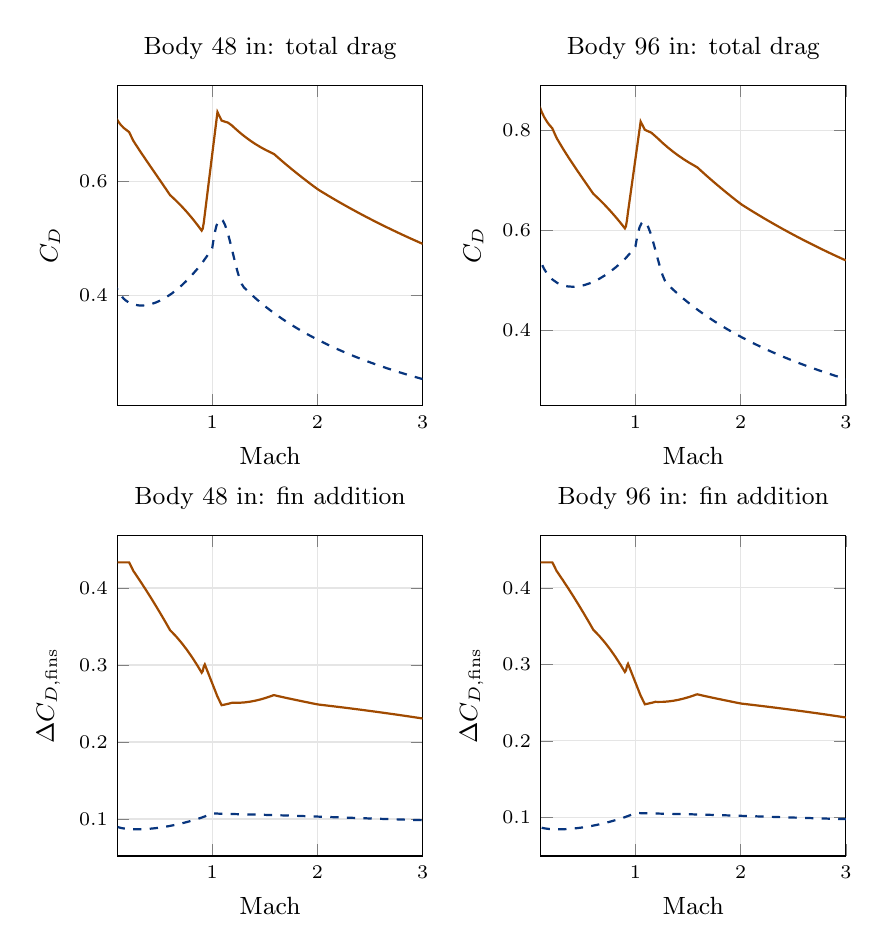
\begin{tikzpicture}
\begin{groupplot}[group style={group size=2 by 2,horizontal sep=1.50cm,vertical sep=1.65cm},width=.45\textwidth,height=5.65cm,grid=major,grid style={gray!20},tick label style={font=\scriptsize},label style={font=\small},title style={font=\small},scaled y ticks=false,yticklabel style={/pgf/number format/fixed,/pgf/number format/precision=3},unbounded coords=jump]
\nextgroupplot[title={Body 48 in: total drag},xlabel={Mach},ylabel={$C_D$},xmin=0.1,xmax=3]
\addplot[thick,B,dashed] coordinates {(0.01,0.5392703) (0.02,0.4900503) (0.03,0.4658697) (0.04,0.450449) (0.05,0.4393925) (0.06,0.4309168) (0.07,0.424134) (0.08,0.4185425) (0.09,0.4138331) (0.11,0.4063117) (0.13,0.4005716) (0.16,0.3941944) (0.18,0.3910132) (0.21,0.3874247) (0.23,0.3856667) (0.26,0.3838032) (0.31,0.3823806) (0.36,0.3826665) (0.41,0.3843774) (0.46,0.3873356) (0.51,0.3914235) (0.56,0.3965597) (0.61,0.4026861) (0.66,0.40976) (0.71,0.4177495) (0.76,0.4266305) (0.81,0.4363845) (0.86,0.4469972) (0.91,0.4585945) (0.96,0.4716979) (1,0.4829383) (1.01,0.4948939) (1.02,0.5066529) (1.04,0.5223558) (1.06,0.531185) (1.08,0.5340179) (1.1,0.5317335) (1.11,0.5282184) (1.12,0.5247436) (1.14,0.5143528) (1.16,0.5014411) (1.18,0.4868895) (1.21,0.4639718) (1.22,0.4563939) (1.24,0.442215) (1.26,0.4299264) (1.28,0.420412) (1.3,0.4145561) (1.31,0.4127028) (1.36,0.4037825) (1.41,0.3953943) (1.46,0.3874794) (1.51,0.3799903) (1.56,0.3728856) (1.61,0.3661305) (1.66,0.3596946) (1.71,0.3535516) (1.76,0.3476781) (1.81,0.342054) (1.86,0.3366609) (1.91,0.3314828) (1.96,0.3265051) (2.01,0.321715) (2.06,0.3171006) (2.11,0.3126512) (2.16,0.3083573) (2.21,0.3042101) (2.26,0.3002013) (2.31,0.2963238) (2.36,0.2925705) (2.41,0.2889353) (2.46,0.2854124) (2.51,0.2819964) (2.56,0.2786823) (2.61,0.2754654) (2.66,0.2723414) (2.71,0.2693063) (2.76,0.2663562) (2.81,0.2634875) (2.86,0.2606971) (2.91,0.2579816) (2.96,0.2553382) (3,0.2532734)};
\addplot[thick,burntorange] coordinates {(0.01,0.8080247) (0.02,0.7703703) (0.03,0.7516897) (0.04,0.7397161) (0.05,0.7310909) (0.06,0.7244427) (0.07,0.7190856) (0.08,0.7146313) (0.09,0.71084) (0.11,0.7046646) (0.13,0.6997837) (0.16,0.6940281) (0.21,0.6869798) (0.25,0.6717458) (0.26,0.6688288) (0.31,0.6546548) (0.36,0.6409243) (0.41,0.6274162) (0.46,0.6139917) (0.51,0.6005588) (0.56,0.5870533) (0.6,0.5761646) (0.61,0.5745601) (0.66,0.5659074) (0.71,0.5565273) (0.76,0.5463991) (0.81,0.5355068) (0.86,0.5238373) (0.9,0.5139346) (0.91,0.5174294) (0.92,0.5279136) (0.96,0.5879089) (1.01,0.6623833) (1.05,0.7219628) (1.06,0.7181847) (1.09,0.7070495) (1.11,0.7057831) (1.15,0.7035359) (1.16,0.7021903) (1.19,0.6981246) (1.21,0.6946208) (1.26,0.6864266) (1.31,0.6789658) (1.36,0.6721722) (1.41,0.6659967) (1.46,0.660401) (1.51,0.6553543) (1.56,0.6508322) (1.59,0.6480014) (1.61,0.644709) (1.66,0.6366592) (1.71,0.6288397) (1.76,0.6212208) (1.81,0.6137783) (1.86,0.6064927) (1.91,0.5993475) (1.96,0.5923293) (2.01,0.5856607) (2.06,0.5800016) (2.11,0.5744531) (2.16,0.5690102) (2.21,0.5636688) (2.26,0.5584257) (2.31,0.5532778) (2.36,0.5482225) (2.41,0.5432574) (2.46,0.5383803) (2.51,0.533589) (2.56,0.5288813) (2.61,0.5242552) (2.66,0.5197083) (2.71,0.5152385) (2.76,0.5108433) (2.81,0.5065202) (2.86,0.5022668) (2.91,0.4980803) (2.96,0.4939578) (3,0.4907041)};
\nextgroupplot[title={Body 96 in: total drag},xlabel={Mach},ylabel={$C_D$},xmin=0.1,xmax=3]
\addplot[thick,B,dashed] coordinates {(0.01,0.7273738) (0.02,0.6564276) (0.03,0.6211958) (0.04,0.5985699) (0.05,0.5822523) (0.06,0.5696742) (0.07,0.5595515) (0.08,0.5511564) (0.09,0.5440394) (0.11,0.5325471) (0.13,0.5236171) (0.16,0.5134037) (0.18,0.5081012) (0.21,0.5017856) (0.26,0.4944524) (0.31,0.4899997) (0.36,0.4877001) (0.41,0.4871314) (0.46,0.4880287) (0.51,0.4902159) (0.56,0.4935707) (0.61,0.4980054) (0.66,0.5034551) (0.71,0.5098711) (0.76,0.5172161) (0.81,0.5254612) (0.86,0.5345837) (0.91,0.5447831) (0.96,0.5568877) (1,0.5674238) (1.01,0.5792175) (1.02,0.5908203) (1.04,0.6062292) (1.06,0.6147894) (1.08,0.6173796) (1.1,0.6148797) (1.11,0.6111324) (1.12,0.6074261) (1.14,0.5965744) (1.16,0.5832048) (1.18,0.5681979) (1.21,0.5446023) (1.24,0.5221734) (1.26,0.5094399) (1.28,0.499483) (1.3,0.4931871) (1.31,0.4911147) (1.36,0.4811076) (1.41,0.4716469) (1.46,0.4626737) (1.51,0.4541401) (1.56,0.4460045) (1.61,0.4382323) (1.66,0.4307927) (1.71,0.4236596) (1.76,0.4168095) (1.81,0.4102224) (1.86,0.4038798) (1.91,0.3977659) (1.96,0.3918659) (2.01,0.3861671) (2.06,0.3806577) (2.11,0.3753269) (2.16,0.3701652) (2.21,0.3651636) (2.26,0.3603141) (2.31,0.3556093) (2.36,0.3510422) (2.41,0.3466065) (2.46,0.3422963) (2.51,0.3381062) (2.56,0.334031) (2.61,0.330066) (2.66,0.3262067) (2.71,0.3224489) (2.76,0.3187887) (2.81,0.3152223) (2.86,0.3117464) (2.91,0.3083575) (2.96,0.3050526) (3,0.3024671)};
\addplot[thick,burntorange] coordinates {(0.01,1.015253) (0.02,0.9515559) (0.03,0.9194443) (0.04,0.8986429) (0.05,0.8835372) (0.06,0.8718165) (0.07,0.8623189) (0.08,0.8543828) (0.09,0.8475982) (0.11,0.8364843) (0.13,0.8276406) (0.16,0.8171376) (0.18,0.8114099) (0.21,0.8041543) (0.25,0.7852738) (0.26,0.7815529) (0.31,0.7638456) (0.36,0.7472001) (0.41,0.731221) (0.46,0.7156585) (0.51,0.7003454) (0.56,0.6851654) (0.6,0.6730592) (0.61,0.6711652) (0.66,0.6611442) (0.71,0.6505125) (0.76,0.6392323) (0.81,0.6272736) (0.86,0.6146122) (0.9,0.6039635) (0.91,0.6080704) (0.92,0.6203913) (0.93,0.6371479) (0.96,0.6822435) (1.01,0.757403) (1.05,0.8175305) (1.06,0.8133815) (1.09,0.8011455) (1.11,0.799155) (1.15,0.7954809) (1.16,0.7937829) (1.21,0.7844759) (1.26,0.7745824) (1.31,0.7654576) (1.36,0.7570325) (1.41,0.7492557) (1.46,0.7420866) (1.51,0.7354926) (1.56,0.7294477) (1.59,0.7257143) (1.61,0.7218245) (1.66,0.7122962) (1.71,0.7030182) (1.76,0.69396) (1.81,0.685096) (1.86,0.676406) (1.91,0.6678725) (1.96,0.6594811) (2.01,0.6515266) (2.06,0.644876) (2.11,0.6383515) (2.16,0.6319483) (2.21,0.6256622) (2.26,0.61949) (2.31,0.6134284) (2.36,0.607475) (2.41,0.601627) (2.46,0.5958823) (2.51,0.5902385) (2.56,0.5846934) (2.61,0.5792446) (2.66,0.5738898) (2.71,0.5686267) (2.76,0.5634525) (2.81,0.5583648) (2.86,0.5533607) (2.91,0.5484373) (2.96,0.5435916) (3,0.539769)};
\nextgroupplot[title={Body 48 in: fin addition},xlabel={Mach},ylabel={$\Delta C_{D,\mathrm{fins}}$},xmin=0.1,xmax=3]
\addplot[thick,B,dashed] coordinates {(0.01,0.1068853) (0.02,0.1003426) (0.03,0.09713073) (0.04,0.095085) (0.05,0.09362091) (0.06,0.09250135) (0.07,0.09160826) (0.08,0.09087493) (0.09,0.09026025) (0.1,0.08973723) (0.11,0.08928726) (0.12,0.088897) (0.13,0.08855661) (0.14,0.0882586) (0.16,0.08776783) (0.18,0.0873912) (0.21,0.08699402) (0.23,0.08682059) (0.26,0.0866739) (0.28,0.0866422) (0.31,0.08668192) (0.33,0.08676146) (0.36,0.08695368) (0.38,0.08712744) (0.41,0.08745243) (0.43,0.08771012) (0.46,0.08815564) (0.48,0.08849075) (0.51,0.0890489) (0.53,0.08945719) (0.56,0.09012279) (0.58,0.09060144) (0.61,0.09137107) (0.66,0.09278976) (0.71,0.0943764) (0.76,0.09612974) (0.81,0.0980494) (0.86,0.1001357) (0.89,0.1014679) (0.91,0.1024078) (0.94,0.103902) (0.96,0.1049376) (1,0.1071052) (1.01,0.1072905) (1.06,0.1070153) (1.11,0.1068473) (1.16,0.1066319) (1.21,0.1064484) (1.26,0.1062793) (1.31,0.1061139) (1.36,0.1059459) (1.41,0.1057716) (1.46,0.1055892) (1.51,0.1053981) (1.56,0.1051984) (1.61,0.1049904) (1.66,0.1047749) (1.71,0.1045527) (1.76,0.1043248) (1.81,0.1040919) (1.86,0.103855) (1.91,0.1036149) (1.96,0.1033723) (2.01,0.1031278) (2.06,0.1028822) (2.11,0.1026359) (2.16,0.1023895) (2.21,0.1021435) (2.26,0.1018982) (2.31,0.101654) (2.36,0.1014111) (2.41,0.10117) (2.46,0.1009307) (2.51,0.1006936) (2.56,0.1004588) (2.61,0.1002264) (2.66,0.09999666) (2.71,0.09976957) (2.76,0.09954526) (2.81,0.09932382) (2.86,0.0991053) (2.91,0.09888975) (2.96,0.09867721) (3,0.09850936)};
\addplot[thick,burntorange] coordinates {(0.01,0.4332722) (0.04,0.4332722) (0.06,0.4332722) (0.11,0.4332722) (0.16,0.4332722) (0.21,0.4332722) (0.22,0.4307899) (0.25,0.4222829) (0.26,0.4202926) (0.31,0.4101517) (0.36,0.3996973) (0.41,0.3889292) (0.46,0.3778472) (0.51,0.3664517) (0.56,0.3547425) (0.6,0.3451492) (0.61,0.3438513) (0.66,0.3366405) (0.71,0.3285687) (0.76,0.3196359) (0.81,0.3098421) (0.86,0.2991874) (0.9,0.2900436) (0.91,0.2920159) (0.92,0.2979327) (0.93,0.3006364) (0.96,0.2902325) (1.01,0.2728926) (1.05,0.2590206) (1.06,0.2561949) (1.09,0.2478347) (1.11,0.2483546) (1.16,0.2499176) (1.19,0.2510356) (1.21,0.2509212) (1.26,0.2509833) (1.31,0.2514913) (1.36,0.2524038) (1.41,0.2536927) (1.46,0.2553375) (1.51,0.2573229) (1.56,0.2596379) (1.58,0.2606544) (1.59,0.2608206) (1.61,0.2601684) (1.66,0.2585993) (1.71,0.2570967) (1.76,0.255639) (1.81,0.2542095) (1.86,0.2527949) (1.91,0.2513849) (1.96,0.2499716) (2.01,0.2486797) (2.06,0.2478809) (2.11,0.2470728) (2.16,0.2462537) (2.21,0.2454226) (2.26,0.2445788) (2.31,0.2437221) (2.36,0.2428523) (2.41,0.2419695) (2.46,0.2410738) (2.51,0.2401653) (2.56,0.2392442) (2.61,0.2383102) (2.66,0.2373635) (2.71,0.2364037) (2.76,0.2354305) (2.81,0.2344434) (2.86,0.2334418) (2.91,0.2324248) (2.96,0.2313916) (3,0.2305527)};
\nextgroupplot[title={Body 96 in: fin addition},xlabel={Mach},ylabel={$\Delta C_{D,\mathrm{fins}}$},xmin=0.1,xmax=3]
\addplot[thick,B,dashed] coordinates {(0.01,0.1012407) (0.02,0.09579145) (0.03,0.09309086) (0.04,0.09136245) (0.05,0.09012211) (0.06,0.08917236) (0.07,0.0884145) (0.08,0.08779257) (0.09,0.08727202) (0.1,0.0868301) (0.11,0.0864511) (0.12,0.08612374) (0.13,0.08583969) (0.14,0.08559261) (0.16,0.08519074) (0.18,0.08488968) (0.21,0.08458774) (0.23,0.08446873) (0.26,0.08439353) (0.27,0.08439312) (0.31,0.08450088) (0.33,0.08461496) (0.36,0.08485472) (0.38,0.08505775) (0.41,0.08542362) (0.43,0.08570683) (0.46,0.08618838) (0.48,0.08654622) (0.51,0.08713676) (0.56,0.08826085) (0.61,0.08955551) (0.66,0.09101754) (0.71,0.0926451) (0.76,0.09443741) (0.81,0.09639446) (0.86,0.09851688) (0.89,0.09987017) (0.91,0.1008225) (0.94,0.1023324) (0.96,0.1033778) (1,0.1055637) (1.01,0.1057532) (1.06,0.1054974) (1.11,0.1053478) (1.16,0.1051587) (1.21,0.1050007) (1.26,0.1048565) (1.31,0.1047154) (1.36,0.104571) (1.41,0.1044199) (1.46,0.1042601) (1.51,0.1040911) (1.56,0.1039129) (1.61,0.1037261) (1.66,0.1035313) (1.71,0.1033294) (1.76,0.1031214) (1.81,0.102908) (1.86,0.1026901) (1.91,0.1024687) (1.96,0.1022443) (2.01,0.1020178) (2.06,0.1017897) (2.11,0.1015607) (2.16,0.1013312) (2.21,0.1011017) (2.26,0.1008726) (2.31,0.1006442) (2.36,0.100417) (2.41,0.100191) (2.46,0.09996674) (2.51,0.09974425) (2.56,0.09952377) (2.61,0.09930544) (2.66,0.09908942) (2.71,0.09887581) (2.76,0.09866471) (2.81,0.09845621) (2.86,0.09825036) (2.91,0.09804723) (2.96,0.09784686) (3,0.09768856)};
\addplot[thick,burntorange] coordinates {(0.01,0.4332722) (0.03,0.4332722) (0.06,0.4332722) (0.11,0.4332722) (0.16,0.4332722) (0.21,0.4332722) (0.22,0.4307899) (0.25,0.4222829) (0.26,0.4202926) (0.31,0.4101519) (0.36,0.3996973) (0.41,0.3889292) (0.46,0.3778474) (0.51,0.3664517) (0.56,0.3547425) (0.6,0.3451492) (0.61,0.3438513) (0.66,0.3366405) (0.71,0.3285687) (0.76,0.3196359) (0.81,0.3098421) (0.86,0.2991874) (0.9,0.2900436) (0.91,0.2920159) (0.92,0.2979327) (0.93,0.3006364) (0.96,0.2902325) (1.01,0.2728926) (1.05,0.2590207) (1.06,0.2561949) (1.09,0.2478347) (1.11,0.2483546) (1.16,0.2499176) (1.19,0.2510356) (1.21,0.2509212) (1.26,0.2509833) (1.31,0.2514913) (1.36,0.2524038) (1.41,0.2536927) (1.46,0.2553375) (1.51,0.2573229) (1.56,0.2596379) (1.58,0.2606544) (1.59,0.2608206) (1.61,0.2601684) (1.66,0.2585993) (1.71,0.2570967) (1.76,0.255639) (1.81,0.2542095) (1.86,0.2527949) (1.91,0.2513849) (1.96,0.2499716) (2.01,0.2486797) (2.06,0.2478809) (2.11,0.2470728) (2.16,0.2462537) (2.21,0.2454226) (2.26,0.2445788) (2.31,0.2437221) (2.36,0.2428523) (2.41,0.2419695) (2.46,0.2410738) (2.51,0.2401653) (2.56,0.2392442) (2.61,0.2383102) (2.66,0.2373635) (2.71,0.2364037) (2.76,0.2354305) (2.81,0.2344434) (2.86,0.2334418) (2.91,0.2324248) (2.96,0.2313916) (3,0.2305527)};
\end{groupplot}\end{tikzpicture}
\caption{Only the cylindrical body length changes. Net fin additions expose the influence of the skin-friction reference length.}\label{fig:atlas-16-fin-length-invariance}
\end{figure}
\noindent{\footnotesize Export files: \code{16-fin-length-invariance.svg} and \code{16-fin-length-invariance.png}.\\ Directory: \code{aerodynamic-investigation/extended/figures/}.}

\clearpage\subsubsection*{Physical roughness: Hbody}
\begin{figure}[H]\centering
{\footnotesize\begin{tabular}{ll}
\tikz[baseline=-.5ex]{\draw[thick,atlasgray,dashed] (0,0)--(.40,0);}\ OR native nearest finish & \tikz[baseline=-.5ex]{\draw[thick,burntorange] (0,0)--(.40,0);}\ RASAero\\
\tikz[baseline=-.5ex]{\draw[thick,B,dashed] (0,0)--(.40,0);}\ OR exact roughness (reconstructed)\\
\end{tabular}}\par\vspace{.7em}
\begin{tikzpicture}
\begin{groupplot}[group style={group size=2 by 2,horizontal sep=1.50cm,vertical sep=1.65cm},width=.45\textwidth,height=5.65cm,grid=major,grid style={gray!20},tick label style={font=\scriptsize},label style={font=\small},title style={font=\small},scaled y ticks=false,yticklabel style={/pgf/number format/fixed,/pgf/number format/precision=3},unbounded coords=jump]
\nextgroupplot[title={RAS roughness 1.27 micrometers},xlabel={Mach},ylabel={$C_D$},xmin=0.1,xmax=3]
\addplot[thick,atlasgray,dashed] coordinates {(0.01,0.432385) (0.02,0.3897077) (0.03,0.368739) (0.04,0.355364) (0.05,0.3457716) (0.06,0.3384154) (0.07,0.3325257) (0.08,0.3276676) (0.09,0.3235729) (0.11,0.3170244) (0.13,0.312015) (0.16,0.3064266) (0.18,0.303622) (0.21,0.3004307) (0.26,0.2971293) (0.31,0.2956987) (0.36,0.2957129) (0.41,0.296925) (0.46,0.29918) (0.51,0.3023746) (0.56,0.3064369) (0.61,0.311315) (0.66,0.3169702) (0.71,0.3233731) (0.76,0.3305008) (0.81,0.3383351) (0.86,0.3468615) (0.91,0.3561867) (0.96,0.3667604) (1,0.3758332) (1.01,0.3876035) (1.02,0.3994312) (1.04,0.41525) (1.06,0.4241697) (1.08,0.4270714) (1.1,0.424837) (1.11,0.4213711) (1.12,0.4179431) (1.14,0.4076398) (1.16,0.3948092) (1.18,0.3803337) (1.21,0.3575234) (1.22,0.34998) (1.24,0.3358689) (1.26,0.323647) (1.28,0.3141988) (1.3,0.308409) (1.31,0.3065889) (1.36,0.2978366) (1.41,0.2896227) (1.46,0.2818902) (1.51,0.2745922) (1.56,0.2676872) (1.61,0.2611402) (1.66,0.2549197) (1.71,0.2489988) (1.76,0.2433533) (1.81,0.2379621) (1.86,0.2328059) (1.91,0.2278679) (1.96,0.2231329) (2.01,0.2185872) (2.06,0.2142184) (2.11,0.2100153) (2.16,0.2059678) (2.21,0.2020666) (2.26,0.1983031) (2.31,0.1946698) (2.36,0.1911594) (2.41,0.1877654) (2.46,0.1844817) (2.51,0.1813028) (2.56,0.1782235) (2.61,0.175239) (2.66,0.1723447) (2.71,0.1695367) (2.76,0.1668109) (2.81,0.1641637) (2.86,0.1615918) (2.91,0.1590919) (2.96,0.156661) (3,0.154764)};
\addplot[thick,burntorange] coordinates {(0.01,0.3747526) (0.02,0.3370981) (0.03,0.3184175) (0.04,0.3064439) (0.05,0.2978187) (0.06,0.2911705) (0.07,0.2858134) (0.08,0.2813592) (0.09,0.2775679) (0.11,0.2713925) (0.13,0.2665116) (0.16,0.2607559) (0.18,0.2576371) (0.21,0.2537077) (0.26,0.2485362) (0.31,0.2445031) (0.36,0.2412271) (0.41,0.238487) (0.46,0.2361445) (0.51,0.2341071) (0.56,0.2323107) (0.61,0.2307088) (0.66,0.2292669) (0.71,0.2279585) (0.76,0.2267632) (0.81,0.2256647) (0.86,0.2246499) (0.9,0.2238911) (0.91,0.2254135) (0.92,0.2299809) (0.93,0.2425879) (0.96,0.2976764) (1.01,0.3894907) (1.05,0.4629422) (1.06,0.4619899) (1.11,0.4574285) (1.15,0.4539954) (1.16,0.4522726) (1.21,0.4436996) (1.26,0.4354433) (1.31,0.4274746) (1.36,0.4197684) (1.41,0.412304) (1.46,0.4050635) (1.51,0.3980314) (1.56,0.3911943) (1.61,0.3845406) (1.66,0.3780599) (1.71,0.371743) (1.76,0.3655817) (1.81,0.3595688) (1.86,0.3536978) (1.91,0.3479626) (1.96,0.3423577) (2.01,0.336981) (2.06,0.3321207) (2.11,0.3273803) (2.16,0.3227565) (2.21,0.3182462) (2.26,0.3138469) (2.31,0.3095557) (2.36,0.3053702) (2.41,0.3012879) (2.46,0.2973064) (2.51,0.2934237) (2.56,0.2896372) (2.61,0.2859449) (2.66,0.2823448) (2.71,0.2788348) (2.76,0.2754128) (2.81,0.2720768) (2.86,0.2688251) (2.91,0.2656555) (2.96,0.2625662) (3,0.2601514)};
\addplot[thick,B,dashed] coordinates {(0.01,0.432385) (0.02,0.3897077) (0.03,0.368739) (0.04,0.355364) (0.05,0.3457716) (0.06,0.3384154) (0.07,0.3325257) (0.08,0.3276676) (0.09,0.3235729) (0.11,0.3170244) (0.13,0.312015) (0.16,0.3064266) (0.18,0.303622) (0.21,0.3004307) (0.26,0.2971293) (0.31,0.2956987) (0.36,0.2957129) (0.41,0.296925) (0.46,0.29918) (0.51,0.3023746) (0.56,0.3064369) (0.61,0.311315) (0.66,0.3169702) (0.71,0.3233731) (0.76,0.3305008) (0.81,0.3383351) (0.86,0.3468615) (0.91,0.3561867) (0.96,0.3667604) (1,0.3758332) (1.01,0.3876035) (1.02,0.3994312) (1.04,0.41525) (1.06,0.4241697) (1.08,0.4270714) (1.1,0.424837) (1.11,0.4213711) (1.12,0.4179431) (1.14,0.4076398) (1.16,0.3948092) (1.18,0.3803337) (1.21,0.3575234) (1.22,0.34998) (1.24,0.3358689) (1.26,0.323647) (1.28,0.3141988) (1.3,0.308409) (1.31,0.3065889) (1.36,0.2978366) (1.41,0.2896227) (1.46,0.2818902) (1.51,0.2745922) (1.56,0.2676872) (1.61,0.2611402) (1.66,0.2549197) (1.71,0.2489988) (1.76,0.2433533) (1.81,0.2379621) (1.86,0.2328059) (1.91,0.2278679) (1.96,0.2231329) (2.01,0.2185872) (2.06,0.2142184) (2.11,0.2100153) (2.16,0.2059678) (2.21,0.2020666) (2.26,0.1983031) (2.31,0.1946698) (2.36,0.1911594) (2.41,0.1877654) (2.46,0.1844817) (2.51,0.1813028) (2.56,0.1782235) (2.61,0.175239) (2.66,0.1723447) (2.71,0.1695367) (2.76,0.1668109) (2.81,0.1641637) (2.86,0.1615918) (2.91,0.1590919) (2.96,0.156661) (3,0.154764)};
\nextgroupplot[title={RAS roughness 6.35 micrometers},xlabel={Mach},ylabel={$C_D$},xmin=0.1,xmax=3]
\addplot[thick,atlasgray,dashed] coordinates {(0.01,0.432385) (0.02,0.3897077) (0.03,0.368739) (0.04,0.355364) (0.05,0.3457716) (0.06,0.3384154) (0.07,0.3325257) (0.08,0.3276676) (0.09,0.3235729) (0.11,0.3170244) (0.13,0.312015) (0.16,0.3064266) (0.18,0.303622) (0.21,0.3004307) (0.26,0.2971293) (0.31,0.2956987) (0.36,0.2957129) (0.41,0.296925) (0.46,0.29918) (0.51,0.3023746) (0.56,0.3064369) (0.61,0.311315) (0.63,0.3135482) (0.66,0.3180136) (0.71,0.3259176) (0.76,0.3343986) (0.81,0.3434565) (0.86,0.3530913) (0.9,0.3612145) (0.91,0.3628526) (0.96,0.371433) (1,0.3787654) (1.01,0.390079) (1.02,0.4014412) (1.04,0.4163012) (1.06,0.4242241) (1.08,0.4270714) (1.1,0.424837) (1.11,0.4213711) (1.12,0.4179431) (1.14,0.4076398) (1.16,0.3948092) (1.18,0.3803337) (1.21,0.3575234) (1.22,0.34998) (1.24,0.3358689) (1.26,0.323647) (1.28,0.3141988) (1.3,0.308409) (1.31,0.3065889) (1.36,0.2978366) (1.41,0.2896227) (1.46,0.2818902) (1.51,0.2745922) (1.56,0.2676872) (1.61,0.2611402) (1.66,0.2549197) (1.71,0.2489988) (1.76,0.2433533) (1.81,0.2379621) (1.86,0.2328059) (1.91,0.2278679) (1.96,0.2231329) (2.01,0.2185872) (2.06,0.2142184) (2.11,0.2100153) (2.16,0.2059678) (2.21,0.2020666) (2.26,0.1983031) (2.31,0.1946698) (2.36,0.1911594) (2.41,0.1877654) (2.46,0.1844817) (2.51,0.1813028) (2.56,0.1782235) (2.61,0.175239) (2.66,0.1723447) (2.71,0.1695367) (2.76,0.1668109) (2.81,0.1641637) (2.86,0.1615918) (2.91,0.1590919) (2.96,0.156661) (3,0.154764)};
\addplot[thick,burntorange] coordinates {(0.01,0.3747526) (0.02,0.3370981) (0.03,0.3184175) (0.04,0.3064439) (0.05,0.2978187) (0.06,0.2911705) (0.07,0.2858134) (0.08,0.2813592) (0.09,0.2775679) (0.11,0.2713925) (0.13,0.2665116) (0.16,0.2607559) (0.18,0.2576371) (0.21,0.2537077) (0.26,0.2485362) (0.31,0.2445031) (0.36,0.2412271) (0.41,0.238487) (0.46,0.2361445) (0.51,0.2341071) (0.52,0.2337303) (0.56,0.2335337) (0.61,0.2333558) (0.66,0.2331801) (0.71,0.2330063) (0.76,0.2328345) (0.81,0.2326647) (0.86,0.2324969) (0.9,0.2323639) (0.91,0.233944) (0.92,0.2386842) (0.93,0.2515445) (0.96,0.3073749) (1.01,0.4004257) (1.05,0.4748663) (1.06,0.4738328) (1.11,0.4688825) (1.15,0.4651569) (1.16,0.4633634) (1.21,0.4544495) (1.26,0.445872) (1.31,0.4375995) (1.36,0.429605) (1.41,0.4218662) (1.46,0.4143636) (1.51,0.4070806) (1.56,0.4000027) (1.61,0.3931175) (1.66,0.3864138) (1.71,0.3798815) (1.76,0.3735119) (1.81,0.3672972) (1.86,0.3612304) (1.91,0.355305) (1.96,0.349515) (2.01,0.3438963) (2.06,0.338573) (2.11,0.3334086) (2.16,0.3283956) (2.21,0.3235272) (2.26,0.3187974) (2.31,0.3142008) (2.36,0.3097325) (2.41,0.3053877) (2.46,0.3011624) (2.51,0.2970525) (2.56,0.2930544) (2.61,0.2891646) (2.66,0.2853797) (2.71,0.2816969) (2.76,0.2781131) (2.81,0.2746253) (2.86,0.271231) (2.91,0.2679275) (2.96,0.2647122) (3,0.262202)};
\addplot[thick,B,dashed] coordinates {(0.01,0.432385) (0.02,0.3897077) (0.03,0.368739) (0.04,0.355364) (0.05,0.3457716) (0.06,0.3384154) (0.07,0.3325257) (0.08,0.3276676) (0.09,0.3235729) (0.11,0.3170244) (0.13,0.312015) (0.16,0.3064266) (0.18,0.303622) (0.21,0.3004307) (0.26,0.2971293) (0.31,0.2956987) (0.36,0.2957129) (0.41,0.296925) (0.46,0.29918) (0.51,0.3047322) (0.56,0.3108672) (0.61,0.3175754) (0.66,0.3248571) (0.71,0.3327121) (0.76,0.3411404) (0.81,0.3501422) (0.86,0.3597172) (0.9,0.3677901) (0.91,0.3693932) (0.96,0.3777986) (1,0.3849909) (1.01,0.3962695) (1.02,0.4075967) (1.04,0.4223867) (1.06,0.4302396) (1.08,0.4320351) (1.1,0.4286533) (1.11,0.4251362) (1.12,0.4216546) (1.14,0.4112373) (1.16,0.3982839) (1.18,0.3836775) (1.21,0.3606564) (1.22,0.3530392) (1.24,0.3387754) (1.26,0.3263944) (1.28,0.3167812) (1.3,0.3108207) (1.31,0.3089134) (1.36,0.2997071) (1.41,0.2910134) (1.46,0.2827803) (1.51,0.2749654) (1.56,0.2676872) (1.61,0.2611402) (1.66,0.2549197) (1.71,0.2489988) (1.76,0.2433533) (1.81,0.2379621) (1.86,0.2328059) (1.91,0.2278679) (1.96,0.2231329) (2.01,0.2185872) (2.06,0.2142184) (2.11,0.2100153) (2.16,0.2059678) (2.21,0.2020666) (2.26,0.1983031) (2.31,0.1946698) (2.36,0.1911594) (2.41,0.1877654) (2.46,0.1844817) (2.51,0.1813028) (2.56,0.1782235) (2.61,0.175239) (2.66,0.1723447) (2.71,0.1695367) (2.76,0.1668109) (2.81,0.1641637) (2.86,0.1615918) (2.91,0.1590919) (2.96,0.156661) (3,0.154764)};
\nextgroupplot[title={RAS roughness 30.48 micrometers},xlabel={Mach},ylabel={$C_D$},xmin=0.1,xmax=3]
\addplot[thick,atlasgray,dashed] coordinates {(0.01,0.432385) (0.02,0.3897077) (0.03,0.368739) (0.04,0.355364) (0.05,0.3457716) (0.06,0.3384154) (0.07,0.3325257) (0.08,0.3276676) (0.09,0.3235729) (0.11,0.3170244) (0.12,0.3160349) (0.16,0.3172749) (0.21,0.3193232) (0.26,0.3219251) (0.31,0.3250805) (0.36,0.3287896) (0.41,0.3330522) (0.46,0.3378685) (0.51,0.3432383) (0.56,0.3491617) (0.61,0.3556387) (0.66,0.3626693) (0.71,0.3702535) (0.76,0.3783913) (0.81,0.3870827) (0.86,0.3963276) (0.9,0.4041222) (0.91,0.4055319) (0.96,0.4129702) (1,0.4193888) (1.01,0.430474) (1.02,0.4416078) (1.04,0.4560109) (1.06,0.463477) (1.08,0.4648857) (1.1,0.4611171) (1.11,0.4574942) (1.12,0.4539067) (1.14,0.4432767) (1.16,0.4301098) (1.18,0.415289) (1.21,0.391945) (1.22,0.3842199) (1.24,0.3697398) (1.26,0.3571421) (1.28,0.3473117) (1.3,0.3411339) (1.31,0.3391177) (1.36,0.3293669) (1.41,0.3201286) (1.46,0.311352) (1.51,0.3029957) (1.56,0.2950229) (1.61,0.2874031) (1.66,0.2801088) (1.71,0.2731167) (1.76,0.2664057) (1.81,0.2599573) (1.86,0.253755) (1.91,0.2477842) (1.96,0.2420312) (2.01,0.2364842) (2.06,0.2311321) (2.11,0.225965) (2.16,0.2209736) (2.21,0.2161494) (2.26,0.2114846) (2.31,0.206972) (2.36,0.2026048) (2.41,0.1983766) (2.46,0.1942816) (2.51,0.1903142) (2.56,0.1864692) (2.61,0.1827416) (2.66,0.1791269) (2.71,0.1756206) (2.76,0.1722185) (2.81,0.1689168) (2.86,0.1657115) (2.91,0.1625992) (2.96,0.1595765) (3,0.1572205)};
\addplot[thick,burntorange] coordinates {(0.01,0.3747526) (0.02,0.3370981) (0.03,0.3184175) (0.04,0.3064439) (0.05,0.2978187) (0.06,0.2911705) (0.07,0.2858134) (0.08,0.2813592) (0.09,0.2775679) (0.1,0.2769812) (0.11,0.2769174) (0.16,0.2766012) (0.21,0.2762889) (0.26,0.2759807) (0.31,0.2756762) (0.36,0.2753756) (0.41,0.2750786) (0.46,0.2747853) (0.51,0.2744954) (0.56,0.2742091) (0.61,0.2739261) (0.66,0.2736464) (0.71,0.27337) (0.76,0.2730968) (0.81,0.2728267) (0.86,0.2725596) (0.9,0.2723481) (0.91,0.2742) (0.92,0.2797559) (0.93,0.2933673) (0.96,0.3500341) (1.01,0.4444787) (1.05,0.5200343) (1.06,0.5187762) (1.11,0.5127321) (1.15,0.508164) (1.16,0.5061641) (1.21,0.4962417) (1.26,0.4866922) (1.31,0.4774808) (1.36,0.4685775) (1.41,0.4599574) (1.46,0.4515989) (1.51,0.4434833) (1.56,0.4355944) (1.61,0.4279181) (1.66,0.4204418) (1.71,0.4131543) (1.76,0.4060458) (1.81,0.3991072) (1.86,0.3923308) (1.91,0.385709) (1.96,0.3792354) (2.01,0.3729474) (2.06,0.3669815) (2.11,0.3612011) (2.16,0.3555965) (2.21,0.3501588) (2.26,0.3448807) (2.31,0.3397551) (2.36,0.334776) (2.41,0.3299373) (2.46,0.3252341) (2.51,0.3206616) (2.56,0.316215) (2.61,0.3118904) (2.66,0.3076837) (2.71,0.3035913) (2.76,0.2996096) (2.81,0.2957352) (2.86,0.291965) (2.91,0.2882959) (2.96,0.284725) (3,0.2819371)};
\addplot[thick,B,dashed] coordinates {(0.01,0.432385) (0.02,0.3897077) (0.03,0.368739) (0.04,0.355364) (0.05,0.3457716) (0.06,0.3384154) (0.07,0.3325257) (0.08,0.3320909) (0.11,0.3327124) (0.16,0.3341842) (0.21,0.3362011) (0.26,0.3387631) (0.31,0.3418703) (0.36,0.3455225) (0.41,0.3497199) (0.46,0.3544624) (0.51,0.35975) (0.56,0.3655827) (0.61,0.3719606) (0.66,0.3788835) (0.71,0.3863516) (0.76,0.3943648) (0.81,0.4029231) (0.86,0.4120265) (0.9,0.4197017) (0.91,0.4210284) (0.96,0.428052) (1,0.4341389) (1.01,0.4451412) (1.02,0.456192) (1.04,0.4704293) (1.06,0.4777295) (1.08,0.4789723) (1.1,0.4750378) (1.11,0.4713696) (1.12,0.4677366) (1.14,0.4570155) (1.16,0.443757) (1.18,0.4288443) (1.21,0.4053618) (1.22,0.3975904) (1.24,0.3830176) (1.26,0.3703269) (1.28,0.3604034) (1.3,0.3541324) (1.31,0.3520695) (1.36,0.3420852) (1.41,0.3326135) (1.46,0.3236038) (1.51,0.3150153) (1.56,0.3068115) (1.61,0.2989624) (1.66,0.2914407) (1.71,0.2842235) (1.76,0.2772897) (1.81,0.2706214) (1.86,0.2642021) (1.91,0.2580172) (1.96,0.2520535) (2.01,0.2462992) (2.06,0.2407433) (2.11,0.235376) (2.16,0.2301879) (2.21,0.2251709) (2.26,0.220317) (2.31,0.2156191) (2.36,0.2110704) (2.41,0.2066646) (2.46,0.2023957) (2.51,0.1982582) (2.56,0.1942469) (2.61,0.1903568) (2.66,0.1865832) (2.71,0.1829217) (2.76,0.179368) (2.81,0.1759183) (2.86,0.1725685) (2.91,0.1693151) (2.96,0.1661547) (3,0.163691)};
\nextgroupplot[title={RAS roughness 152.4 micrometers},xlabel={Mach},ylabel={$C_D$},xmin=0.1,xmax=3]
\addplot[thick,atlasgray,dashed] coordinates {(0.01,0.432385) (0.02,0.4101727) (0.06,0.4104964) (0.11,0.4113562) (0.16,0.4127217) (0.21,0.414593) (0.26,0.41697) (0.31,0.4198527) (0.36,0.4232412) (0.41,0.4271354) (0.46,0.4315354) (0.51,0.4364411) (0.56,0.4418526) (0.61,0.4477698) (0.66,0.4541928) (0.71,0.4611215) (0.76,0.4685559) (0.81,0.4764961) (0.86,0.484942) (0.9,0.4920629) (0.91,0.4930044) (0.96,0.4981019) (1,0.502648) (1.01,0.513265) (1.02,0.5239306) (1.04,0.5373975) (1.06,0.5439272) (1.08,0.5443995) (1.1,0.5396947) (1.11,0.535816) (1.12,0.5319719) (1.14,0.5208273) (1.16,0.5071434) (1.18,0.4918037) (1.21,0.4676782) (1.24,0.4446882) (1.26,0.4315659) (1.28,0.42121) (1.3,0.4145058) (1.31,0.4122263) (1.36,0.4011575) (1.41,0.3906012) (1.46,0.3805091) (1.51,0.370842) (1.56,0.3615657) (1.61,0.3526514) (1.66,0.3440736) (1.71,0.3358104) (1.76,0.3278423) (1.81,0.3201523) (1.86,0.3127247) (1.91,0.3055461) (1.96,0.2986037) (2.01,0.2918865) (2.06,0.2853838) (2.11,0.2790864) (2.16,0.2729854) (2.21,0.2670726) (2.26,0.2613405) (2.31,0.2557819) (2.36,0.2503902) (2.41,0.2451592) (2.46,0.2400827) (2.51,0.2351553) (2.56,0.2303715) (2.61,0.2257264) (2.66,0.2212149) (2.71,0.2168326) (2.76,0.2125749) (2.81,0.2084376) (2.86,0.2044167) (2.91,0.2005081) (2.96,0.1967082) (3,0.1937441)};
\addplot[thick,burntorange] coordinates {(0.01,0.3747526) (0.02,0.3468211) (0.06,0.3463966) (0.11,0.3458724) (0.16,0.345355) (0.21,0.3448442) (0.26,0.34434) (0.31,0.3438422) (0.36,0.3433506) (0.41,0.3428652) (0.46,0.3423857) (0.51,0.341912) (0.56,0.3414441) (0.61,0.3409817) (0.66,0.3405249) (0.71,0.3400734) (0.76,0.3396271) (0.81,0.339186) (0.86,0.3387499) (0.9,0.3384046) (0.91,0.3407058) (0.92,0.3476092) (0.93,0.3622358) (0.96,0.4189299) (1.01,0.51342) (1.05,0.589012) (1.06,0.5873915) (1.11,0.5795862) (1.15,0.5736659) (1.16,0.5713352) (1.21,0.5597998) (1.26,0.5487003) (1.31,0.5379959) (1.36,0.5276516) (1.41,0.5176378) (1.46,0.5079291) (1.51,0.4985032) (1.56,0.4893409) (1.61,0.4804254) (1.66,0.4717416) (1.71,0.463276) (1.76,0.4550169) (1.81,0.4469535) (1.86,0.4390764) (1.91,0.4313766) (1.96,0.4238462) (2.01,0.4165205) (2.06,0.409541) (2.11,0.4027915) (2.16,0.3962585) (2.21,0.38993) (2.26,0.3837956) (2.31,0.3778458) (2.36,0.3720724) (2.41,0.3664675) (2.46,0.3610244) (2.51,0.3557366) (2.56,0.3505981) (2.61,0.3456036) (2.66,0.3407479) (2.71,0.3360264) (2.76,0.3314346) (2.81,0.326968) (2.86,0.3226229) (2.91,0.3183954) (2.96,0.3142818) (3,0.3110706)};
\addplot[thick,B,dashed] coordinates {(0.01,0.432385) (0.02,0.4110901) (0.06,0.4114135) (0.11,0.4122725) (0.16,0.4136367) (0.21,0.4155063) (0.26,0.4178811) (0.31,0.4207613) (0.36,0.4241467) (0.41,0.4280374) (0.46,0.4324334) (0.51,0.4373346) (0.56,0.4427412) (0.61,0.448653) (0.66,0.4550702) (0.71,0.4619926) (0.76,0.4694203) (0.81,0.4773533) (0.86,0.4857916) (0.9,0.492906) (0.91,0.493843) (0.96,0.4989181) (1,0.5034461) (1.01,0.5140587) (1.02,0.5247198) (1.04,0.5381777) (1.06,0.5446985) (1.08,0.5451618) (1.1,0.540448) (1.11,0.5365668) (1.12,0.5327203) (1.14,0.5215707) (1.16,0.5078819) (1.18,0.4925372) (1.21,0.4684043) (1.24,0.4454067) (1.26,0.4322794) (1.28,0.4219184) (1.3,0.4152093) (1.31,0.4129272) (1.36,0.4018457) (1.41,0.3912768) (1.46,0.3811721) (1.51,0.3714925) (1.56,0.3622036) (1.61,0.3532769) (1.66,0.3446868) (1.71,0.3364114) (1.76,0.3284313) (1.81,0.3207293) (1.86,0.3132901) (1.91,0.3060998) (1.96,0.2991461) (2.01,0.2924176) (2.06,0.2859039) (2.11,0.2795957) (2.16,0.273484) (2.21,0.2675608) (2.26,0.2618185) (2.31,0.2562499) (2.36,0.2508484) (2.41,0.2456077) (2.46,0.2405218) (2.51,0.2355852) (2.56,0.2307924) (2.61,0.2261385) (2.66,0.2216184) (2.71,0.2172277) (2.76,0.2129618) (2.81,0.2088165) (2.86,0.2047877) (2.91,0.2008715) (2.96,0.1970642) (3,0.1940942)};
\end{groupplot}\end{tikzpicture}
\caption{Gray: native OR nearest available finish (2, 5, 20, 150 micrometers respectively). Blue: native OR correlation reconstructed at the exact RAS roughness, verified against all native finish curves; no OR application changes.}\label{fig:atlas-17-roughness-Hbody}
\end{figure}
\noindent{\footnotesize Export files: \code{17-roughness-Hbody.svg} and \code{17-roughness-Hbody.png}.\\ Directory: \code{aerodynamic-investigation/extended/figures/}.}

\clearpage\subsubsection*{Physical roughness: Hsq}
\begin{figure}[H]\centering
{\footnotesize\begin{tabular}{ll}
\tikz[baseline=-.5ex]{\draw[thick,atlasgray,dashed] (0,0)--(.40,0);}\ OR native nearest finish & \tikz[baseline=-.5ex]{\draw[thick,burntorange] (0,0)--(.40,0);}\ RASAero\\
\tikz[baseline=-.5ex]{\draw[thick,B,dashed] (0,0)--(.40,0);}\ OR exact roughness (reconstructed)\\
\end{tabular}}\par\vspace{.7em}
\begin{tikzpicture}
\begin{groupplot}[group style={group size=2 by 2,horizontal sep=1.50cm,vertical sep=1.65cm},width=.45\textwidth,height=5.65cm,grid=major,grid style={gray!20},tick label style={font=\scriptsize},label style={font=\small},title style={font=\small},scaled y ticks=false,yticklabel style={/pgf/number format/fixed,/pgf/number format/precision=3},unbounded coords=jump]
\nextgroupplot[title={RAS roughness 1.27 micrometers},xlabel={Mach},ylabel={$C_D$},xmin=0.1,xmax=3]
\addplot[thick,atlasgray,dashed] coordinates {(0.01,0.5392703) (0.02,0.4900503) (0.03,0.4658697) (0.04,0.450449) (0.05,0.4393925) (0.06,0.4309168) (0.07,0.424134) (0.08,0.4185425) (0.09,0.4138331) (0.11,0.4063117) (0.13,0.4005716) (0.16,0.3941944) (0.18,0.3910132) (0.21,0.3874247) (0.23,0.3856667) (0.26,0.3838032) (0.31,0.3823806) (0.36,0.3826665) (0.41,0.3843774) (0.46,0.3873356) (0.51,0.3914235) (0.56,0.3965597) (0.61,0.4026861) (0.66,0.40976) (0.71,0.4177495) (0.76,0.4266305) (0.81,0.4363845) (0.86,0.4469972) (0.91,0.4585945) (0.96,0.4716979) (1,0.4829383) (1.01,0.4948939) (1.02,0.5066529) (1.04,0.5223558) (1.06,0.531185) (1.08,0.5340179) (1.1,0.5317335) (1.11,0.5282184) (1.12,0.5247436) (1.14,0.5143528) (1.16,0.5014411) (1.18,0.4868895) (1.21,0.4639718) (1.22,0.4563939) (1.24,0.442215) (1.26,0.4299264) (1.28,0.420412) (1.3,0.4145561) (1.31,0.4127028) (1.36,0.4037825) (1.41,0.3953943) (1.46,0.3874794) (1.51,0.3799903) (1.56,0.3728856) (1.61,0.3661305) (1.66,0.3596946) (1.71,0.3535516) (1.76,0.3476781) (1.81,0.342054) (1.86,0.3366609) (1.91,0.3314828) (1.96,0.3265051) (2.01,0.321715) (2.06,0.3171006) (2.11,0.3126512) (2.16,0.3083573) (2.21,0.3042101) (2.26,0.3002013) (2.31,0.2963238) (2.36,0.2925705) (2.41,0.2889353) (2.46,0.2854124) (2.51,0.2819964) (2.56,0.2786823) (2.61,0.2754654) (2.66,0.2723414) (2.71,0.2693063) (2.76,0.2663562) (2.81,0.2634875) (2.86,0.2606971) (2.91,0.2579816) (2.96,0.2553382) (3,0.2532734)};
\addplot[thick,burntorange] coordinates {(0.01,0.8080247) (0.02,0.7703703) (0.03,0.7516897) (0.04,0.7397161) (0.05,0.7310909) (0.06,0.7244427) (0.07,0.7190856) (0.08,0.7146313) (0.09,0.71084) (0.11,0.7046646) (0.13,0.6997837) (0.16,0.6940281) (0.21,0.6869798) (0.25,0.6717458) (0.26,0.6688288) (0.31,0.6546548) (0.36,0.6409243) (0.41,0.6274162) (0.46,0.6139917) (0.51,0.6005588) (0.56,0.5870533) (0.6,0.5761646) (0.61,0.5745601) (0.66,0.5659074) (0.71,0.5565273) (0.76,0.5463991) (0.81,0.5355068) (0.86,0.5238373) (0.9,0.5139346) (0.91,0.5174294) (0.92,0.5279136) (0.96,0.5879089) (1.01,0.6623833) (1.05,0.7219628) (1.06,0.7181847) (1.09,0.7070495) (1.11,0.7057831) (1.15,0.7035359) (1.16,0.7021903) (1.19,0.6981246) (1.21,0.6946208) (1.26,0.6864266) (1.31,0.6789658) (1.36,0.6721722) (1.41,0.6659967) (1.46,0.660401) (1.51,0.6553543) (1.56,0.6508322) (1.59,0.6480014) (1.61,0.644709) (1.66,0.6366592) (1.71,0.6288397) (1.76,0.6212208) (1.81,0.6137783) (1.86,0.6064927) (1.91,0.5993475) (1.96,0.5923293) (2.01,0.5856607) (2.06,0.5800016) (2.11,0.5744531) (2.16,0.5690102) (2.21,0.5636688) (2.26,0.5584257) (2.31,0.5532778) (2.36,0.5482225) (2.41,0.5432574) (2.46,0.5383803) (2.51,0.533589) (2.56,0.5288813) (2.61,0.5242552) (2.66,0.5197083) (2.71,0.5152385) (2.76,0.5108433) (2.81,0.5065202) (2.86,0.5022668) (2.91,0.4980803) (2.96,0.4939578) (3,0.4907041)};
\addplot[thick,B,dashed] coordinates {(0.01,0.5392703) (0.02,0.4900503) (0.03,0.4658697) (0.04,0.450449) (0.05,0.4393925) (0.06,0.4309168) (0.07,0.424134) (0.08,0.4185425) (0.09,0.4138331) (0.11,0.4063117) (0.13,0.4005716) (0.16,0.3941944) (0.18,0.3910132) (0.21,0.3874247) (0.23,0.3856667) (0.26,0.3838032) (0.31,0.3823806) (0.36,0.3826665) (0.41,0.3843774) (0.46,0.3873356) (0.51,0.3914235) (0.56,0.3965597) (0.61,0.4026861) (0.66,0.40976) (0.71,0.4177495) (0.76,0.4266305) (0.81,0.4363845) (0.86,0.4469972) (0.91,0.4585945) (0.96,0.4716979) (1,0.4829383) (1.01,0.4948939) (1.02,0.5066529) (1.04,0.5223558) (1.06,0.531185) (1.08,0.5340179) (1.1,0.5317335) (1.11,0.5282184) (1.12,0.5247436) (1.14,0.5143528) (1.16,0.5014411) (1.18,0.4868895) (1.21,0.4639718) (1.22,0.4563939) (1.24,0.442215) (1.26,0.4299264) (1.28,0.420412) (1.3,0.4145561) (1.31,0.4127028) (1.36,0.4037825) (1.41,0.3953943) (1.46,0.3874794) (1.51,0.3799903) (1.56,0.3728856) (1.61,0.3661305) (1.66,0.3596946) (1.71,0.3535516) (1.76,0.3476781) (1.81,0.342054) (1.86,0.3366609) (1.91,0.3314828) (1.96,0.3265051) (2.01,0.321715) (2.06,0.3171006) (2.11,0.3126512) (2.16,0.3083573) (2.21,0.3042101) (2.26,0.3002013) (2.31,0.2963238) (2.36,0.2925705) (2.41,0.2889353) (2.46,0.2854124) (2.51,0.2819964) (2.56,0.2786823) (2.61,0.2754654) (2.66,0.2723414) (2.71,0.2693063) (2.76,0.2663562) (2.81,0.2634875) (2.86,0.2606971) (2.91,0.2579816) (2.96,0.2553382) (3,0.2532734)};
\nextgroupplot[title={RAS roughness 6.35 micrometers},xlabel={Mach},ylabel={$C_D$},xmin=0.1,xmax=3]
\addplot[thick,atlasgray,dashed] coordinates {(0.01,0.5392703) (0.02,0.4900503) (0.03,0.4658697) (0.04,0.450449) (0.05,0.4393925) (0.06,0.4309168) (0.07,0.424134) (0.08,0.4185425) (0.09,0.4138331) (0.11,0.4063117) (0.13,0.4005716) (0.16,0.3941944) (0.18,0.3910132) (0.21,0.3874247) (0.23,0.3856667) (0.26,0.3838032) (0.31,0.3823806) (0.36,0.3826665) (0.41,0.3843774) (0.46,0.3873356) (0.51,0.3914235) (0.56,0.3965597) (0.61,0.4026861) (0.63,0.405476) (0.66,0.4109634) (0.71,0.4206843) (0.76,0.4311261) (0.81,0.4422913) (0.86,0.4541824) (0.9,0.4642199) (0.91,0.4662827) (0.96,0.4770872) (1,0.4863202) (1.01,0.4977492) (1.02,0.5089711) (1.04,0.5235682) (1.06,0.5312478) (1.08,0.5340179) (1.1,0.5317335) (1.11,0.5282184) (1.12,0.5247436) (1.14,0.5143528) (1.16,0.5014411) (1.18,0.4868895) (1.21,0.4639718) (1.22,0.4563939) (1.24,0.442215) (1.26,0.4299264) (1.28,0.420412) (1.3,0.4145561) (1.31,0.4127028) (1.36,0.4037825) (1.41,0.3953943) (1.46,0.3874794) (1.51,0.3799903) (1.56,0.3728856) (1.61,0.3661305) (1.66,0.3596946) (1.71,0.3535516) (1.76,0.3476781) (1.81,0.342054) (1.86,0.3366609) (1.91,0.3314828) (1.96,0.3265051) (2.01,0.321715) (2.06,0.3171006) (2.11,0.3126512) (2.16,0.3083573) (2.21,0.3042101) (2.26,0.3002013) (2.31,0.2963238) (2.36,0.2925705) (2.41,0.2889353) (2.46,0.2854124) (2.51,0.2819964) (2.56,0.2786823) (2.61,0.2754654) (2.66,0.2723414) (2.71,0.2693063) (2.76,0.2663562) (2.81,0.2634875) (2.86,0.2606971) (2.91,0.2579816) (2.96,0.2553382) (3,0.2532734)};
\addplot[thick,burntorange] coordinates {(0.01,0.8080247) (0.02,0.7703703) (0.03,0.7516897) (0.04,0.7397161) (0.05,0.7310909) (0.06,0.7244427) (0.07,0.7190856) (0.08,0.7146313) (0.09,0.71084) (0.11,0.7046646) (0.13,0.6997837) (0.16,0.6940281) (0.21,0.6869798) (0.25,0.6717458) (0.26,0.6688288) (0.31,0.6546548) (0.36,0.6409243) (0.41,0.6274162) (0.46,0.6139917) (0.51,0.6005588) (0.56,0.5882762) (0.6,0.5785404) (0.61,0.5772071) (0.66,0.5698206) (0.71,0.561575) (0.76,0.5524705) (0.81,0.5425068) (0.86,0.5316843) (0.9,0.5224075) (0.91,0.5259598) (0.92,0.536617) (0.93,0.5521809) (0.96,0.5976074) (1.01,0.6733183) (1.05,0.7338869) (1.06,0.7300277) (1.09,0.7186558) (1.11,0.7172371) (1.15,0.7146974) (1.16,0.713281) (1.19,0.7090083) (1.21,0.7053707) (1.26,0.6968553) (1.31,0.6890908) (1.36,0.6820088) (1.41,0.6755589) (1.46,0.6697011) (1.51,0.6644034) (1.56,0.6596406) (1.59,0.65667) (1.61,0.653286) (1.66,0.6450131) (1.71,0.6369782) (1.76,0.629151) (1.81,0.6215067) (1.86,0.6140253) (1.91,0.6066899) (1.96,0.5994866) (2.01,0.5925759) (2.06,0.5864538) (2.11,0.5804814) (2.16,0.5746494) (2.21,0.5689498) (2.26,0.5633763) (2.31,0.5579229) (2.36,0.5525848) (2.41,0.5473572) (2.46,0.5422362) (2.51,0.5372179) (2.56,0.5322985) (2.61,0.5274748) (2.66,0.5227433) (2.71,0.5181006) (2.76,0.5135436) (2.81,0.5090687) (2.86,0.5046728) (2.91,0.5003523) (2.96,0.4961039) (3,0.4927547)};
\addplot[thick,B,dashed] coordinates {(0.01,0.5392703) (0.02,0.4900503) (0.03,0.4658697) (0.04,0.450449) (0.05,0.4393925) (0.06,0.4309168) (0.07,0.424134) (0.08,0.4185425) (0.09,0.4138331) (0.11,0.4063117) (0.13,0.4005716) (0.16,0.3941944) (0.18,0.3910132) (0.21,0.3874247) (0.23,0.3856667) (0.26,0.3838032) (0.31,0.3823806) (0.36,0.3826665) (0.41,0.3843774) (0.46,0.3873356) (0.51,0.3941427) (0.56,0.4016694) (0.61,0.4099066) (0.66,0.4188564) (0.71,0.4285207) (0.76,0.4389019) (0.81,0.4500023) (0.86,0.4618245) (0.9,0.4718039) (0.91,0.4738264) (0.96,0.484429) (1,0.4935005) (1.01,0.5048891) (1.02,0.5160706) (1.04,0.530587) (1.06,0.5381858) (1.08,0.5397428) (1.1,0.5361351) (1.11,0.5325609) (1.12,0.5290243) (1.14,0.5185019) (1.16,0.5054487) (1.18,0.4907461) (1.21,0.4675853) (1.22,0.4599222) (1.24,0.4455671) (1.26,0.4330951) (1.28,0.4233903) (1.3,0.4173377) (1.31,0.4153838) (1.36,0.4059398) (1.41,0.3969983) (1.46,0.388506) (1.51,0.3804208) (1.56,0.3728856) (1.61,0.3661305) (1.66,0.3596946) (1.71,0.3535516) (1.76,0.3476781) (1.81,0.342054) (1.86,0.3366609) (1.91,0.3314828) (1.96,0.3265051) (2.01,0.321715) (2.06,0.3171006) (2.11,0.3126512) (2.16,0.3083573) (2.21,0.3042101) (2.26,0.3002013) (2.31,0.2963238) (2.36,0.2925705) (2.41,0.2889353) (2.46,0.2854124) (2.51,0.2819964) (2.56,0.2786823) (2.61,0.2754654) (2.66,0.2723414) (2.71,0.2693063) (2.76,0.2663562) (2.81,0.2634875) (2.86,0.2606971) (2.91,0.2579816) (2.96,0.2553382) (3,0.2532734)};
\nextgroupplot[title={RAS roughness 30.48 micrometers},xlabel={Mach},ylabel={$C_D$},xmin=0.1,xmax=3]
\addplot[thick,atlasgray,dashed] coordinates {(0.01,0.5392703) (0.02,0.4900503) (0.03,0.4658697) (0.04,0.450449) (0.05,0.4393925) (0.06,0.4309168) (0.07,0.424134) (0.08,0.4185425) (0.09,0.4138331) (0.11,0.4063117) (0.12,0.4051884) (0.16,0.4067065) (0.21,0.4092146) (0.26,0.4124017) (0.31,0.4162685) (0.36,0.420816) (0.41,0.4260452) (0.46,0.4319574) (0.51,0.4385541) (0.56,0.4458368) (0.61,0.4538073) (0.66,0.4624676) (0.71,0.4718196) (0.76,0.4818656) (0.81,0.4926081) (0.86,0.5040496) (0.9,0.5137079) (0.91,0.5155073) (0.96,0.5249945) (1,0.5331737) (1.01,0.5443392) (1.02,0.5552977) (1.04,0.5693679) (1.06,0.5765205) (1.08,0.5776314) (1.1,0.5735775) (1.11,0.5698815) (1.12,0.5662226) (1.14,0.555455) (1.16,0.5421554) (1.18,0.5272056) (1.21,0.5036723) (1.22,0.4958848) (1.24,0.4812803) (1.26,0.4685582) (1.28,0.4586031) (1.3,0.4522997) (1.31,0.4502203) (1.36,0.4401483) (1.41,0.4305786) (1.46,0.4214596) (1.51,0.4127498) (1.56,0.4044135) (1.61,0.3964212) (1.66,0.3887467) (1.71,0.3813682) (1.76,0.3742658) (1.81,0.3674225) (1.86,0.3608229) (1.91,0.3544534) (1.96,0.3483017) (2.01,0.3423567) (2.06,0.3366082) (2.11,0.331047) (2.16,0.3256644) (2.21,0.3204527) (2.26,0.3154043) (2.31,0.3105127) (2.36,0.3057712) (2.41,0.3011739) (2.46,0.2967152) (2.51,0.2923898) (2.56,0.2881925) (2.61,0.2841187) (2.66,0.2801637) (2.71,0.2763232) (2.76,0.2725931) (2.81,0.2689695) (2.86,0.2654487) (2.91,0.2620269) (2.96,0.2587008) (3,0.2561066)};
\addplot[thick,burntorange] coordinates {(0.01,0.8080247) (0.02,0.7703703) (0.03,0.7516897) (0.04,0.7397161) (0.05,0.7310909) (0.06,0.7244427) (0.07,0.7190856) (0.08,0.7146313) (0.09,0.71084) (0.11,0.7101896) (0.16,0.7098733) (0.21,0.7095611) (0.25,0.6983249) (0.26,0.6962732) (0.31,0.6858279) (0.36,0.6750729) (0.41,0.6640078) (0.46,0.6526324) (0.51,0.6409471) (0.56,0.6289516) (0.6,0.6191316) (0.61,0.6177774) (0.66,0.6102869) (0.71,0.6019387) (0.76,0.5927327) (0.81,0.5826687) (0.86,0.571747) (0.9,0.5623916) (0.91,0.5662159) (0.92,0.5776887) (0.93,0.5940037) (0.96,0.6402665) (1.01,0.7173712) (1.05,0.779055) (1.06,0.7749711) (1.09,0.7629372) (1.11,0.7610867) (1.15,0.7577045) (1.16,0.7560817) (1.19,0.7511994) (1.21,0.7471629) (1.26,0.7376755) (1.31,0.728972) (1.36,0.7209813) (1.41,0.7136501) (1.46,0.7069364) (1.51,0.7008062) (1.56,0.6952323) (1.59,0.6917846) (1.61,0.6880865) (1.66,0.6790412) (1.71,0.670251) (1.76,0.6616848) (1.81,0.6533167) (1.86,0.6451256) (1.91,0.6370939) (1.96,0.6292069) (2.01,0.621627) (2.06,0.6148624) (2.11,0.6082739) (2.16,0.6018502) (2.21,0.5955814) (2.26,0.5894595) (2.31,0.5834772) (2.36,0.5776283) (2.41,0.5719068) (2.46,0.5663079) (2.51,0.5608269) (2.56,0.5554592) (2.61,0.5502006) (2.66,0.5450472) (2.71,0.539995) (2.76,0.5350401) (2.81,0.5301786) (2.86,0.5254068) (2.91,0.5207207) (2.96,0.5161166) (3,0.5124898)};
\addplot[thick,B,dashed] coordinates {(0.01,0.5392703) (0.02,0.4900503) (0.03,0.4658697) (0.04,0.450449) (0.05,0.4393925) (0.06,0.4309168) (0.07,0.424134) (0.08,0.4236442) (0.11,0.4244055) (0.16,0.4262089) (0.21,0.4286809) (0.26,0.431822) (0.31,0.4356331) (0.36,0.4401151) (0.41,0.445269) (0.46,0.4510962) (0.51,0.4575981) (0.56,0.4647762) (0.61,0.4726323) (0.66,0.4811684) (0.71,0.4903864) (0.76,0.5002888) (0.81,0.5108778) (0.86,0.522156) (0.9,0.5316766) (0.91,0.5333804) (0.96,0.5423893) (1,0.5501859) (1.01,0.5612557) (1.02,0.5721186) (1.04,0.5859974) (1.06,0.5929588) (1.08,0.5938783) (1.1,0.5896332) (1.11,0.5858848) (1.12,0.5821736) (1.14,0.5713008) (1.16,0.5578956) (1.18,0.5428397) (1.21,0.5191468) (1.24,0.4965944) (1.26,0.4837651) (1.28,0.4737026) (1.3,0.4672916) (1.31,0.4651584) (1.36,0.4548171) (1.41,0.4449782) (1.46,0.4355903) (1.51,0.4266127) (1.56,0.4180101) (1.61,0.4097532) (1.66,0.4018166) (1.71,0.3941783) (1.76,0.386819) (1.81,0.379722) (1.86,0.372872) (1.91,0.3662558) (1.96,0.3598611) (2.01,0.353677) (2.06,0.3476934) (2.11,0.3419012) (2.16,0.3362919) (2.21,0.3308577) (2.26,0.3255913) (2.31,0.3204859) (2.36,0.3155351) (2.41,0.3107329) (2.46,0.3060737) (2.51,0.3015521) (2.56,0.297163) (2.61,0.2929017) (2.66,0.2887634) (2.71,0.284744) (2.76,0.2808391) (2.81,0.2770448) (2.86,0.2733572) (2.91,0.2697728) (2.96,0.2662879) (3,0.2635694)};
\nextgroupplot[title={RAS roughness 152.4 micrometers},xlabel={Mach},ylabel={$C_D$},xmin=0.1,xmax=3]
\addplot[thick,atlasgray,dashed] coordinates {(0.01,0.5392703) (0.02,0.5136539) (0.06,0.5140522) (0.11,0.5151103) (0.16,0.5167911) (0.21,0.519095) (0.26,0.5220227) (0.31,0.525575) (0.36,0.5297527) (0.41,0.5345571) (0.46,0.5399892) (0.51,0.5460506) (0.56,0.5527429) (0.61,0.5600677) (0.66,0.5680271) (0.71,0.5766231) (0.76,0.5858579) (0.81,0.595734) (0.86,0.6062539) (0.9,0.6151353) (0.91,0.6163948) (0.96,0.6231822) (1,0.6292016) (1.01,0.6398271) (1.02,0.6502456) (1.04,0.6632359) (1.06,0.6693087) (1.08,0.6693396) (1.1,0.6642058) (1.11,0.6602147) (1.12,0.65626) (1.14,0.6448987) (1.16,0.631003) (1.18,0.6154547) (1.21,0.59102) (1.24,0.5677229) (1.26,0.5543958) (1.28,0.5438345) (1.3,0.5369241) (1.31,0.5345409) (1.36,0.5229488) (1.41,0.511859) (1.46,0.5012226) (1.51,0.4910012) (1.56,0.4811614) (1.61,0.471676) (1.66,0.4625212) (1.71,0.4536767) (1.76,0.4451244) (1.81,0.436849) (1.86,0.4288362) (1.91,0.4210738) (1.96,0.4135503) (2.01,0.4062555) (2.06,0.39918) (2.11,0.3923152) (2.16,0.3856528) (2.21,0.3791855) (2.26,0.3729062) (2.31,0.3668081) (2.36,0.3608851) (2.41,0.3551311) (2.46,0.3495405) (2.51,0.3441078) (2.56,0.3388278) (2.61,0.3336956) (2.66,0.3287064) (2.71,0.3238555) (2.76,0.3191386) (2.81,0.3145513) (2.86,0.3100896) (2.91,0.3057495) (2.96,0.3015271) (3,0.2982315)};
\addplot[thick,burntorange] coordinates {(0.01,0.8080247) (0.02,0.7800933) (0.06,0.7796688) (0.11,0.7791445) (0.16,0.7786271) (0.21,0.7781164) (0.25,0.7667233) (0.26,0.7646326) (0.31,0.7539939) (0.36,0.7430479) (0.41,0.7317943) (0.46,0.7202328) (0.51,0.7083637) (0.56,0.6961866) (0.6,0.6862229) (0.61,0.684833) (0.66,0.6771654) (0.71,0.6686421) (0.76,0.659263) (0.81,0.6490281) (0.86,0.6379373) (0.9,0.6284482) (0.91,0.6327216) (0.92,0.645542) (0.93,0.6628723) (0.96,0.7091624) (1.01,0.7863125) (1.05,0.8480327) (1.06,0.8435863) (1.09,0.8304859) (1.11,0.8279409) (1.15,0.8232065) (1.16,0.8212529) (1.19,0.8153947) (1.21,0.810721) (1.26,0.7996836) (1.31,0.7894872) (1.36,0.7800554) (1.41,0.7713305) (1.46,0.7632666) (1.51,0.7558261) (1.56,0.7489788) (1.59,0.7447837) (1.61,0.7405938) (1.66,0.7303409) (1.71,0.7203727) (1.76,0.7106559) (1.81,0.701163) (1.86,0.6918713) (1.91,0.6827615) (1.96,0.6738178) (2.01,0.6652002) (2.06,0.6574219) (2.11,0.6498643) (2.16,0.6425123) (2.21,0.6353526) (2.26,0.6283744) (2.31,0.6215679) (2.36,0.6149247) (2.41,0.608437) (2.46,0.6020982) (2.51,0.5959019) (2.56,0.5898422) (2.61,0.5839138) (2.66,0.5781114) (2.71,0.5724301) (2.76,0.5668651) (2.81,0.5614114) (2.86,0.5560647) (2.91,0.5508202) (2.96,0.5456735) (3,0.5416233)};
\addplot[thick,B,dashed] coordinates {(0.01,0.5392703) (0.02,0.5147119) (0.06,0.5151099) (0.11,0.5161671) (0.16,0.5178464) (0.21,0.5201484) (0.26,0.5230737) (0.31,0.5266229) (0.36,0.5307971) (0.41,0.5355973) (0.46,0.5410249) (0.51,0.5470812) (0.56,0.5537678) (0.61,0.5610864) (0.66,0.5690391) (0.71,0.5776278) (0.76,0.5868549) (0.81,0.5967227) (0.86,0.6072338) (0.9,0.6161076) (0.91,0.6173619) (0.96,0.6241235) (1,0.6301222) (1.01,0.6407425) (1.02,0.6511559) (1.04,0.6641358) (1.06,0.6701982) (1.08,0.6702188) (1.1,0.6650747) (1.11,0.6610807) (1.12,0.6571232) (1.14,0.6457562) (1.16,0.6318548) (1.18,0.6163007) (1.21,0.5918574) (1.24,0.5685516) (1.26,0.5552187) (1.28,0.5446516) (1.3,0.5377353) (1.31,0.5353493) (1.36,0.5237426) (1.41,0.5126382) (1.46,0.5019873) (1.51,0.4917513) (1.56,0.4818971) (1.61,0.4723975) (1.66,0.4632284) (1.71,0.4543699) (1.76,0.4458037) (1.81,0.4375145) (1.86,0.4294882) (1.91,0.4217125) (1.96,0.4141758) (2.01,0.4068681) (2.06,0.3997799) (2.11,0.3929025) (2.16,0.3862279) (2.21,0.3797486) (2.26,0.3734574) (2.31,0.3673478) (2.36,0.3614135) (2.41,0.3556484) (2.46,0.3500469) (2.51,0.3446036) (2.56,0.3393133) (2.61,0.3341709) (2.66,0.3291718) (2.71,0.3243112) (2.76,0.3195848) (2.81,0.3149883) (2.86,0.3105176) (2.91,0.3061687) (2.96,0.3019377) (3,0.2986353)};
\end{groupplot}\end{tikzpicture}
\caption{Gray: native OR nearest available finish (2, 5, 20, 150 micrometers respectively). Blue: native OR correlation reconstructed at the exact RAS roughness, verified against all native finish curves; no OR application changes.}\label{fig:atlas-17-roughness-Hsq}
\end{figure}
\noindent{\footnotesize Export files: \code{17-roughness-Hsq.svg} and \code{17-roughness-Hsq.png}.\\ Directory: \code{aerodynamic-investigation/extended/figures/}.}

\clearpage\subsubsection*{Physical roughness: Hbev}
\begin{figure}[H]\centering
{\footnotesize\begin{tabular}{ll}
\tikz[baseline=-.5ex]{\draw[thick,atlasgray,dashed] (0,0)--(.40,0);}\ OR native nearest finish & \tikz[baseline=-.5ex]{\draw[thick,burntorange] (0,0)--(.40,0);}\ RASAero\\
\tikz[baseline=-.5ex]{\draw[thick,B,dashed] (0,0)--(.40,0);}\ OR exact roughness (reconstructed)\\
\end{tabular}}\par\vspace{.7em}
\begin{tikzpicture}
\begin{groupplot}[group style={group size=2 by 2,horizontal sep=1.50cm,vertical sep=1.65cm},width=.45\textwidth,height=5.65cm,grid=major,grid style={gray!20},tick label style={font=\scriptsize},label style={font=\small},title style={font=\small},scaled y ticks=false,yticklabel style={/pgf/number format/fixed,/pgf/number format/precision=3},unbounded coords=jump]
\nextgroupplot[title={RAS roughness 1.27 micrometers},xlabel={Mach},ylabel={$C_D$},xmin=0.1,xmax=3]
\addplot[thick,atlasgray,dashed] coordinates {(0.01,0.4955621) (0.02,0.4463415) (0.03,0.4221597) (0.04,0.4067373) (0.05,0.3956786) (0.06,0.3872002) (0.07,0.3804143) (0.08,0.3748193) (0.09,0.3701059) (0.11,0.3625749) (0.13,0.3568235) (0.16,0.3504259) (0.18,0.3472289) (0.21,0.3436136) (0.23,0.3418356) (0.26,0.3399392) (0.31,0.3384548) (0.36,0.3386713) (0.41,0.3403069) (0.46,0.3431862) (0.51,0.3471947) (0.56,0.3522544) (0.61,0.3583117) (0.66,0.3653296) (0.71,0.3732834) (0.76,0.3821579) (0.81,0.3919458) (0.86,0.4026476) (0.91,0.4144078) (0.96,0.4277726) (1,0.4393144) (1.01,0.4510799) (1.02,0.4629209) (1.04,0.4788217) (1.06,0.4878998) (1.08,0.4910396) (1.1,0.4891272) (1.11,0.4858248) (1.12,0.4825817) (1.14,0.4727157) (1.16,0.4604176) (1.18,0.4465782) (1.21,0.4249381) (1.22,0.4178484) (1.24,0.404751) (1.26,0.3936996) (1.28,0.3856) (1.3,0.3813638) (1.31,0.3804075) (1.34,0.37809) (1.36,0.3770685) (1.39,0.3764987) (1.41,0.376916) (1.43,0.3775066) (1.46,0.3727592) (1.51,0.366726) (1.56,0.3625256) (1.61,0.3594235) (1.66,0.3565539) (1.71,0.3529445) (1.76,0.3476781) (1.81,0.342054) (1.86,0.3366609) (1.91,0.3314828) (1.96,0.3265051) (2.01,0.321715) (2.06,0.3171006) (2.11,0.3126512) (2.16,0.3083573) (2.21,0.3042101) (2.26,0.3002013) (2.31,0.2963238) (2.36,0.2925705) (2.41,0.2889353) (2.46,0.2854124) (2.49,0.2833503) (2.5,0.2430483) (2.51,0.240604) (2.53,0.2374095) (2.56,0.233615) (2.61,0.2282684) (2.66,0.2235344) (2.71,0.2191793) (2.76,0.2151014) (2.81,0.2112445) (2.86,0.2075729) (2.91,0.2040619) (2.96,0.2006932) (3,0.1980912)};
\addplot[thick,burntorange] coordinates {(0.01,0.5863164) (0.02,0.5211986) (0.03,0.4891801) (0.04,0.4687447) (0.05,0.4540613) (0.06,0.442762) (0.07,0.4336675) (0.08,0.4261116) (0.09,0.4196841) (0.1,0.4141154) (0.11,0.4092202) (0.13,0.4009531) (0.14,0.3974088) (0.16,0.3912058) (0.18,0.3859236) (0.21,0.3792669) (0.24,0.3737261) (0.26,0.3706882) (0.31,0.3647434) (0.36,0.3600281) (0.41,0.3561808) (0.46,0.3529754) (0.51,0.3502616) (0.56,0.3479347) (0.6,0.3463006) (0.61,0.3462077) (0.66,0.3458135) (0.71,0.3455966) (0.76,0.3455285) (0.81,0.3455865) (0.86,0.3457523) (0.9,0.3459527) (0.91,0.3483052) (0.92,0.3553626) (0.93,0.3697444) (0.96,0.4242766) (1.01,0.5151636) (1.05,0.5878732) (1.06,0.5866429) (1.11,0.5807182) (1.13,0.5790303) (1.15,0.5780496) (1.16,0.576851) (1.19,0.5736579) (1.21,0.5710699) (1.23,0.5688669) (1.26,0.5662524) (1.28,0.564955) (1.31,0.5636602) (1.33,0.5632242) (1.36,0.5632031) (1.38,0.5636076) (1.41,0.5648392) (1.43,0.5660756) (1.46,0.5685528) (1.49,0.5717779) (1.51,0.5743443) (1.54,0.5788208) (1.56,0.5822248) (1.58,0.5859661) (1.59,0.5858598) (1.61,0.5799547) (1.66,0.5658094) (1.71,0.5524506) (1.76,0.5397811) (1.81,0.5277226) (1.86,0.5162118) (1.91,0.5051956) (1.96,0.4946296) (2.01,0.4846276) (2.06,0.475588) (2.11,0.4669043) (2.16,0.4585525) (2.21,0.4505112) (2.26,0.4427617) (2.31,0.4352867) (2.36,0.4280706) (2.41,0.4210989) (2.46,0.4143585) (2.51,0.4078372) (2.56,0.4015231) (2.61,0.3954055) (2.66,0.3894743) (2.71,0.3837197) (2.76,0.3781323) (2.81,0.3727032) (2.86,0.3674241) (2.91,0.3622866) (2.96,0.3572828) (3,0.3533708)};
\addplot[thick,B,dashed] coordinates {(0.01,0.4955621) (0.02,0.4463415) (0.03,0.4221597) (0.04,0.4067373) (0.05,0.3956786) (0.06,0.3872002) (0.07,0.3804143) (0.08,0.3748193) (0.09,0.3701059) (0.11,0.3625749) (0.13,0.3568235) (0.16,0.3504259) (0.18,0.3472289) (0.21,0.3436136) (0.23,0.3418356) (0.26,0.3399392) (0.31,0.3384548) (0.36,0.3386713) (0.41,0.3403069) (0.46,0.3431862) (0.51,0.3471947) (0.56,0.3522544) (0.61,0.3583117) (0.66,0.3653296) (0.71,0.3732834) (0.76,0.3821579) (0.81,0.3919458) (0.86,0.4026476) (0.91,0.4144078) (0.96,0.4277726) (1,0.4393144) (1.01,0.4510799) (1.02,0.4629209) (1.04,0.4788217) (1.06,0.4878998) (1.08,0.4910396) (1.1,0.4891272) (1.11,0.4858248) (1.12,0.4825817) (1.14,0.4727157) (1.16,0.4604176) (1.18,0.4465782) (1.21,0.4249381) (1.22,0.4178484) (1.24,0.404751) (1.26,0.3936996) (1.28,0.3856) (1.3,0.3813638) (1.31,0.3804075) (1.34,0.37809) (1.36,0.3770685) (1.39,0.3764987) (1.41,0.376916) (1.43,0.3775066) (1.46,0.3727592) (1.51,0.366726) (1.56,0.3625256) (1.61,0.3594235) (1.66,0.3565539) (1.71,0.3529445) (1.76,0.3476781) (1.81,0.342054) (1.86,0.3366609) (1.91,0.3314828) (1.96,0.3265051) (2.01,0.321715) (2.06,0.3171006) (2.11,0.3126512) (2.16,0.3083573) (2.21,0.3042101) (2.26,0.3002013) (2.31,0.2963238) (2.36,0.2925705) (2.41,0.2889353) (2.46,0.2854124) (2.49,0.2833503) (2.5,0.2430483) (2.51,0.240604) (2.53,0.2374095) (2.56,0.233615) (2.61,0.2282684) (2.66,0.2235344) (2.71,0.2191793) (2.76,0.2151014) (2.81,0.2112445) (2.86,0.2075729) (2.91,0.2040619) (2.96,0.2006932) (3,0.1980912)};
\nextgroupplot[title={RAS roughness 6.35 micrometers},xlabel={Mach},ylabel={$C_D$},xmin=0.1,xmax=3]
\addplot[thick,atlasgray,dashed] coordinates {(0.01,0.4955621) (0.02,0.4463415) (0.03,0.4221597) (0.04,0.4067373) (0.05,0.3956786) (0.06,0.3872002) (0.07,0.3804143) (0.08,0.3748193) (0.09,0.3701059) (0.11,0.3625749) (0.13,0.3568235) (0.16,0.3504259) (0.18,0.3472289) (0.21,0.3436136) (0.23,0.3418356) (0.26,0.3399392) (0.31,0.3384548) (0.36,0.3386713) (0.41,0.3403069) (0.46,0.3431862) (0.51,0.3471947) (0.56,0.3522544) (0.61,0.3583117) (0.63,0.3610773) (0.66,0.3665331) (0.71,0.3762182) (0.76,0.3866535) (0.81,0.3978526) (0.86,0.4098328) (0.9,0.4199936) (0.91,0.422096) (0.96,0.4331619) (1,0.4426963) (1.01,0.4539351) (1.02,0.4652391) (1.04,0.4800341) (1.06,0.4879626) (1.08,0.4910396) (1.1,0.4891272) (1.11,0.4858248) (1.12,0.4825817) (1.14,0.4727157) (1.16,0.4604176) (1.18,0.4465782) (1.21,0.4249381) (1.22,0.4178484) (1.24,0.404751) (1.26,0.3936996) (1.28,0.3856) (1.3,0.3813638) (1.31,0.3804075) (1.34,0.37809) (1.36,0.3770685) (1.39,0.3764987) (1.41,0.376916) (1.43,0.3775066) (1.46,0.3727592) (1.51,0.366726) (1.56,0.3625256) (1.61,0.3594235) (1.66,0.3565539) (1.71,0.3529445) (1.76,0.3476781) (1.81,0.342054) (1.86,0.3366609) (1.91,0.3314828) (1.96,0.3265051) (2.01,0.321715) (2.06,0.3171006) (2.11,0.3126512) (2.16,0.3083573) (2.21,0.3042101) (2.26,0.3002013) (2.31,0.2963238) (2.36,0.2925705) (2.41,0.2889353) (2.46,0.2854124) (2.49,0.2833503) (2.5,0.2430483) (2.51,0.240604) (2.53,0.2374095) (2.56,0.233615) (2.61,0.2282684) (2.66,0.2235344) (2.71,0.2191793) (2.76,0.2151014) (2.81,0.2112445) (2.86,0.2075729) (2.91,0.2040619) (2.96,0.2006932) (3,0.1980912)};
\addplot[thick,burntorange] coordinates {(0.01,0.5863164) (0.02,0.5211986) (0.03,0.4891801) (0.04,0.4687447) (0.05,0.4540613) (0.06,0.442762) (0.07,0.4336675) (0.08,0.4261116) (0.09,0.4196841) (0.1,0.4141154) (0.11,0.4092202) (0.13,0.4009531) (0.14,0.3974088) (0.16,0.3912058) (0.18,0.3859236) (0.21,0.3792669) (0.24,0.3737261) (0.26,0.3706882) (0.31,0.3647434) (0.36,0.3600281) (0.41,0.3561808) (0.44,0.3541914) (0.46,0.3535316) (0.51,0.3521977) (0.52,0.3519614) (0.56,0.3523265) (0.61,0.3531536) (0.66,0.3551403) (0.71,0.3571228) (0.76,0.3591013) (0.81,0.3610758) (0.86,0.3630464) (0.9,0.36462) (0.91,0.3670994) (0.92,0.3745377) (0.93,0.3892599) (0.96,0.4441213) (1.01,0.5355569) (1.05,0.6087054) (1.06,0.6073336) (1.11,0.600731) (1.13,0.5987847) (1.15,0.5975523) (1.16,0.5962302) (1.19,0.5926757) (1.21,0.589854) (1.23,0.5874228) (1.26,0.5844756) (1.28,0.5829624) (1.31,0.5813525) (1.36,0.5803912) (1.41,0.5815472) (1.46,0.5848023) (1.51,0.5901546) (1.56,0.5976136) (1.58,0.6011909) (1.59,0.6010036) (1.61,0.5949381) (1.66,0.580402) (1.71,0.5666658) (1.76,0.5536313) (1.81,0.5412192) (1.86,0.5293652) (1.91,0.5180157) (1.96,0.5071253) (2.01,0.4967104) (2.06,0.4869128) (2.11,0.4775343) (2.16,0.4685439) (2.21,0.4599142) (2.26,0.4516212) (2.31,0.4436431) (2.36,0.4359604) (2.41,0.428555) (2.46,0.421411) (2.51,0.4145133) (2.56,0.4078478) (2.61,0.4014017) (2.66,0.3951627) (2.71,0.3891196) (2.76,0.3832615) (2.81,0.3775781) (2.86,0.3720597) (2.91,0.3666969) (2.96,0.3614807) (3,0.3574076)};
\addplot[thick,B,dashed] coordinates {(0.01,0.4955621) (0.02,0.4463415) (0.03,0.4221597) (0.04,0.4067373) (0.05,0.3956786) (0.06,0.3872002) (0.07,0.3804143) (0.08,0.3748193) (0.09,0.3701059) (0.11,0.3625749) (0.13,0.3568235) (0.16,0.3504259) (0.18,0.3472289) (0.21,0.3436136) (0.23,0.3418356) (0.26,0.3399392) (0.31,0.3384548) (0.36,0.3386713) (0.41,0.3403069) (0.46,0.3431862) (0.51,0.3499139) (0.56,0.357364) (0.61,0.3655322) (0.66,0.3744261) (0.71,0.3840547) (0.76,0.3944292) (0.81,0.4055636) (0.86,0.4174749) (0.9,0.4275776) (0.91,0.4296397) (0.96,0.4405036) (1,0.4498766) (1.01,0.461075) (1.02,0.4723387) (1.04,0.4870529) (1.06,0.4949006) (1.08,0.4967645) (1.1,0.4935288) (1.11,0.4901673) (1.12,0.4868625) (1.14,0.4768648) (1.16,0.4644252) (1.18,0.4504348) (1.21,0.4285516) (1.22,0.4213767) (1.24,0.4081032) (1.26,0.3968683) (1.28,0.3885784) (1.3,0.3841454) (1.31,0.3830885) (1.34,0.3804607) (1.36,0.3792258) (1.39,0.3783272) (1.41,0.37852) (1.43,0.3788822) (1.46,0.3737859) (1.51,0.3671565) (1.56,0.3625256) (1.61,0.3594235) (1.66,0.3565539) (1.71,0.3529445) (1.76,0.3476781) (1.81,0.342054) (1.86,0.3366609) (1.91,0.3314828) (1.96,0.3265051) (2.01,0.321715) (2.06,0.3171006) (2.11,0.3126512) (2.16,0.3083573) (2.21,0.3042101) (2.26,0.3002013) (2.31,0.2963238) (2.36,0.2925705) (2.41,0.2889353) (2.46,0.2854124) (2.49,0.2833503) (2.5,0.2430483) (2.51,0.240604) (2.53,0.2374095) (2.56,0.233615) (2.61,0.2282684) (2.66,0.2235344) (2.71,0.2191793) (2.76,0.2151014) (2.81,0.2112445) (2.86,0.2075729) (2.91,0.2040619) (2.96,0.2006932) (3,0.1980912)};
\nextgroupplot[title={RAS roughness 30.48 micrometers},xlabel={Mach},ylabel={$C_D$},xmin=0.1,xmax=3]
\addplot[thick,atlasgray,dashed] coordinates {(0.01,0.4955621) (0.02,0.4463415) (0.03,0.4221597) (0.04,0.4067373) (0.05,0.3956786) (0.06,0.3872002) (0.07,0.3804143) (0.08,0.3748193) (0.09,0.3701059) (0.11,0.3625749) (0.12,0.3614462) (0.16,0.3629379) (0.21,0.3654034) (0.26,0.3685377) (0.31,0.3723427) (0.36,0.3768207) (0.41,0.3819746) (0.46,0.3878081) (0.51,0.3943253) (0.56,0.4015315) (0.61,0.409433) (0.66,0.4180372) (0.71,0.4273535) (0.76,0.4373929) (0.81,0.4481694) (0.86,0.4596999) (0.9,0.4694816) (0.91,0.4713206) (0.96,0.4810692) (1,0.4895498) (1.01,0.5005251) (1.02,0.5115657) (1.04,0.5258338) (1.06,0.5332354) (1.08,0.5346531) (1.1,0.5309713) (1.11,0.5274879) (1.12,0.5240608) (1.14,0.5138179) (1.16,0.501132) (1.18,0.4868943) (1.21,0.4646386) (1.22,0.4573393) (1.24,0.4438163) (1.26,0.4323315) (1.28,0.4237911) (1.3,0.4191074) (1.31,0.4179249) (1.36,0.4134342) (1.39,0.4121587) (1.41,0.4121004) (1.43,0.4122117) (1.46,0.4067394) (1.51,0.3994855) (1.56,0.3940536) (1.61,0.3897141) (1.66,0.3856061) (1.71,0.3807611) (1.76,0.3742658) (1.81,0.3674225) (1.86,0.3608229) (1.91,0.3544534) (1.96,0.3483017) (2.01,0.3423567) (2.06,0.3366082) (2.11,0.331047) (2.16,0.3256644) (2.21,0.3204527) (2.26,0.3154043) (2.31,0.3105127) (2.36,0.3057712) (2.41,0.3011739) (2.46,0.2967152) (2.49,0.2941043) (2.5,0.2536214) (2.51,0.2509974) (2.53,0.2474465) (2.56,0.2431253) (2.61,0.2369217) (2.66,0.2313566) (2.71,0.2261962) (2.76,0.2213384) (2.81,0.2167265) (2.86,0.2123245) (2.91,0.2081072) (2.96,0.2040558) (3,0.2009244)};
\addplot[thick,burntorange] coordinates {(0.01,0.5863164) (0.02,0.5211986) (0.03,0.4891801) (0.04,0.4687447) (0.05,0.4540613) (0.06,0.442762) (0.07,0.4336675) (0.08,0.4265535) (0.09,0.4227156) (0.11,0.4219724) (0.16,0.4214265) (0.21,0.4208875) (0.26,0.4205918) (0.31,0.4212457) (0.36,0.4219014) (0.41,0.4225587) (0.46,0.4232176) (0.51,0.4238781) (0.56,0.4245401) (0.6,0.4250708) (0.61,0.4256255) (0.66,0.4283196) (0.71,0.4310073) (0.76,0.4336888) (0.81,0.4363641) (0.86,0.4390333) (0.9,0.4411643) (0.91,0.4441642) (0.92,0.453164) (0.93,0.4688123) (0.96,0.5222036) (1.01,0.6111891) (1.05,0.6823775) (1.06,0.6806244) (1.11,0.6721682) (1.13,0.6695036) (1.15,0.6675652) (1.16,0.6658945) (1.21,0.6578178) (1.26,0.6508039) (1.31,0.6461044) (1.36,0.6436204) (1.41,0.6433026) (1.46,0.6451289) (1.51,0.6490939) (1.56,0.6552037) (1.58,0.6582514) (1.59,0.6578013) (1.61,0.6512144) (1.66,0.6353973) (1.71,0.6204108) (1.76,0.6061543) (1.81,0.592547) (1.86,0.5795229) (1.91,0.5670267) (1.96,0.5550118) (2.01,0.5434936) (2.06,0.5326238) (2.11,0.5222194) (2.16,0.5122456) (2.21,0.5026715) (2.26,0.4934701) (2.31,0.4846171) (2.36,0.4760909) (2.41,0.4678712) (2.46,0.4599404) (2.51,0.4522818) (2.56,0.4448798) (2.61,0.4377203) (2.66,0.43079) (2.71,0.4240764) (2.76,0.4175677) (2.81,0.4112526) (2.86,0.4051207) (2.91,0.3991618) (2.96,0.3933661) (3,0.3888408)};
\addplot[thick,B,dashed] coordinates {(0.01,0.4955621) (0.02,0.4463415) (0.03,0.4221597) (0.04,0.4067373) (0.05,0.3956786) (0.06,0.3872002) (0.07,0.3804143) (0.08,0.379921) (0.11,0.3806688) (0.16,0.3824404) (0.21,0.3848697) (0.26,0.3879581) (0.31,0.3917073) (0.36,0.3961198) (0.41,0.4011985) (0.46,0.4069469) (0.51,0.4133693) (0.56,0.4204709) (0.61,0.4282579) (0.66,0.436738) (0.71,0.4459204) (0.76,0.4558161) (0.81,0.4664391) (0.86,0.4778063) (0.9,0.4874504) (0.91,0.4891937) (0.96,0.498464) (1,0.506562) (1.01,0.5174417) (1.02,0.5283866) (1.04,0.5424634) (1.06,0.5496736) (1.08,0.5509001) (1.1,0.5470269) (1.11,0.5434912) (1.12,0.5400117) (1.14,0.5296637) (1.16,0.5168721) (1.18,0.5025284) (1.21,0.4801131) (1.22,0.4727603) (1.24,0.4591304) (1.26,0.4475384) (1.28,0.4388906) (1.3,0.4340993) (1.31,0.4328631) (1.36,0.4281031) (1.39,0.4266659) (1.41,0.4264999) (1.43,0.4265036) (1.46,0.4208701) (1.51,0.4133485) (1.56,0.4076501) (1.61,0.4030462) (1.66,0.3986759) (1.71,0.3935712) (1.76,0.386819) (1.81,0.379722) (1.86,0.372872) (1.91,0.3662558) (1.96,0.3598611) (2.01,0.353677) (2.06,0.3476934) (2.11,0.3419012) (2.16,0.3362919) (2.21,0.3308577) (2.26,0.3255913) (2.31,0.3204859) (2.36,0.3155351) (2.41,0.3107329) (2.46,0.3060737) (2.49,0.3033446) (2.5,0.2628226) (2.51,0.2601597) (2.53,0.2565316) (2.56,0.2520958) (2.61,0.2457047) (2.66,0.2399564) (2.71,0.234617) (2.76,0.2295843) (2.81,0.2248018) (2.86,0.220233) (2.91,0.215853) (2.96,0.2116429) (3,0.2083872)};
\nextgroupplot[title={RAS roughness 152.4 micrometers},xlabel={Mach},ylabel={$C_D$},xmin=0.1,xmax=3]
\addplot[thick,atlasgray,dashed] coordinates {(0.01,0.4955621) (0.02,0.469945) (0.06,0.4703356) (0.11,0.4713735) (0.16,0.4730225) (0.21,0.4752838) (0.26,0.4781588) (0.31,0.4816492) (0.36,0.4857575) (0.41,0.4904865) (0.46,0.4958398) (0.51,0.5018218) (0.56,0.5084375) (0.61,0.5156933) (0.66,0.5235968) (0.71,0.532157) (0.76,0.5413853) (0.81,0.5512953) (0.86,0.5619043) (0.9,0.570909) (0.91,0.5722081) (0.96,0.5792568) (1,0.5855777) (1.01,0.596013) (1.02,0.6065137) (1.04,0.6197018) (1.06,0.6260235) (1.08,0.6263613) (1.1,0.6215996) (1.11,0.6178211) (1.12,0.6140982) (1.14,0.6032616) (1.16,0.5899795) (1.21,0.5519863) (1.24,0.5302589) (1.26,0.518169) (1.28,0.5090225) (1.3,0.5037318) (1.31,0.5022456) (1.36,0.4962347) (1.39,0.4940469) (1.41,0.4933807) (1.43,0.4928846) (1.46,0.4865024) (1.51,0.4777369) (1.56,0.4708014) (1.61,0.464969) (1.66,0.4593805) (1.71,0.4530696) (1.76,0.4451244) (1.81,0.436849) (1.86,0.4288362) (1.91,0.4210738) (1.96,0.4135503) (2.01,0.4062555) (2.06,0.39918) (2.11,0.3923152) (2.16,0.3856528) (2.21,0.3791855) (2.26,0.3729062) (2.31,0.3668081) (2.36,0.3608851) (2.41,0.3551311) (2.46,0.3495405) (2.49,0.3462623) (2.5,0.3055589) (2.51,0.3027154) (2.53,0.2987285) (2.56,0.2937606) (2.61,0.2864987) (2.66,0.2798993) (2.71,0.2737285) (2.76,0.2678839) (2.81,0.2623083) (2.86,0.2569655) (2.91,0.2518298) (2.96,0.2468821) (3,0.2430493)};
\addplot[thick,burntorange] coordinates {(0.01,0.5863164) (0.02,0.5437703) (0.06,0.5430222) (0.11,0.5420985) (0.16,0.5411869) (0.21,0.5402873) (0.26,0.539748) (0.31,0.5406096) (0.36,0.541474) (0.41,0.5423413) (0.46,0.5432112) (0.51,0.5440838) (0.56,0.5449589) (0.6,0.5456608) (0.61,0.5464572) (0.66,0.5503208) (0.71,0.5541736) (0.76,0.5580158) (0.81,0.5618473) (0.86,0.5656684) (0.9,0.568718) (0.91,0.5725853) (0.92,0.5841871) (0.96,0.6506445) (1.01,0.733153) (1.05,0.7991598) (1.06,0.7967612) (1.11,0.785174) (1.13,0.7812996) (1.15,0.7781739) (1.16,0.7759179) (1.21,0.7649914) (1.26,0.7552471) (1.31,0.7479249) (1.36,0.742916) (1.41,0.7401625) (1.46,0.7396347) (1.51,0.7413203) (1.56,0.7452199) (1.58,0.7474016) (1.59,0.7465222) (1.61,0.739084) (1.66,0.7211795) (1.71,0.7041605) (1.76,0.6879228) (1.81,0.672382) (1.86,0.6574691) (1.91,0.643126) (1.96,0.6293037) (2.01,0.6160055) (2.06,0.6033713) (2.11,0.5912845) (2.16,0.5797028) (2.21,0.5685893) (2.26,0.5579115) (2.31,0.5476404) (2.36,0.5377502) (2.41,0.528217) (2.46,0.51902) (2.51,0.5101394) (2.56,0.5015572) (2.61,0.4932568) (2.66,0.4852229) (2.71,0.4774409) (2.76,0.4698973) (2.81,0.4625791) (2.86,0.4554745) (2.91,0.4485718) (2.96,0.44186) (3,0.4366209)};
\addplot[thick,B,dashed] coordinates {(0.01,0.4955621) (0.02,0.471003) (0.06,0.4713933) (0.11,0.4724303) (0.16,0.4740779) (0.21,0.4763372) (0.26,0.4792097) (0.31,0.4826971) (0.36,0.4868018) (0.41,0.4915268) (0.46,0.4968755) (0.51,0.5028523) (0.56,0.5094624) (0.61,0.516712) (0.66,0.5246088) (0.71,0.5331618) (0.76,0.5423822) (0.81,0.552284) (0.86,0.5628841) (0.9,0.5718814) (0.91,0.5731752) (0.96,0.5801981) (1,0.5864983) (1.01,0.5969285) (1.02,0.6074239) (1.04,0.6206017) (1.06,0.626913) (1.08,0.6272405) (1.1,0.6224684) (1.11,0.6186871) (1.12,0.6149614) (1.14,0.6041191) (1.16,0.5908313) (1.21,0.5528237) (1.24,0.5310877) (1.26,0.5189919) (1.28,0.5098396) (1.3,0.5045431) (1.31,0.503054) (1.36,0.4970285) (1.39,0.494832) (1.41,0.4941599) (1.43,0.493658) (1.46,0.4872671) (1.51,0.4784871) (1.56,0.4715372) (1.61,0.4656905) (1.66,0.4600878) (1.71,0.4537628) (1.76,0.4458037) (1.81,0.4375145) (1.86,0.4294882) (1.91,0.4217125) (1.96,0.4141758) (2.01,0.4068681) (2.06,0.3997799) (2.11,0.3929025) (2.16,0.3862279) (2.21,0.3797486) (2.26,0.3734574) (2.31,0.3673478) (2.36,0.3614135) (2.41,0.3556484) (2.46,0.3500469) (2.49,0.3467623) (2.5,0.3060568) (2.51,0.3032112) (2.53,0.2992201) (2.56,0.294246) (2.61,0.2869739) (2.66,0.2803647) (2.71,0.2741842) (2.76,0.2683301) (2.81,0.2627453) (2.86,0.2573934) (2.91,0.2522489) (2.96,0.2472927) (3,0.2434531)};
\end{groupplot}\end{tikzpicture}
\caption{Gray: native OR nearest available finish (2, 5, 20, 150 micrometers respectively). Blue: native OR correlation reconstructed at the exact RAS roughness, verified against all native finish curves; no OR application changes.}\label{fig:atlas-17-roughness-Hbev}
\end{figure}
\noindent{\footnotesize Export files: \code{17-roughness-Hbev.svg} and \code{17-roughness-Hbev.png}.\\ Directory: \code{aerodynamic-investigation/extended/figures/}.}

\clearpage\subsubsection*{Roughness-induced drag at fixed Mach}
\begin{figure}[H]\centering
{\footnotesize\begin{tabular}{lll}
\tikz[baseline=-.5ex]{\draw[thick,B,dashed] (0,0)--(.40,0);}\ Hbody OR exact k & \tikz[baseline=-.5ex]{\draw[thick,B] (0,0)--(.40,0);}\ Hbody RAS & \tikz[baseline=-.5ex]{\draw[thick,burntorange,dashed] (0,0)--(.40,0);}\ Hsq OR exact k\\
\tikz[baseline=-.5ex]{\draw[thick,burntorange] (0,0)--(.40,0);}\ Hsq RAS & \tikz[baseline=-.5ex]{\draw[thick,g,dashed] (0,0)--(.40,0);}\ Hbev OR exact k & \tikz[baseline=-.5ex]{\draw[thick,g] (0,0)--(.40,0);}\ Hbev RAS\\
\end{tabular}}\par\vspace{.7em}
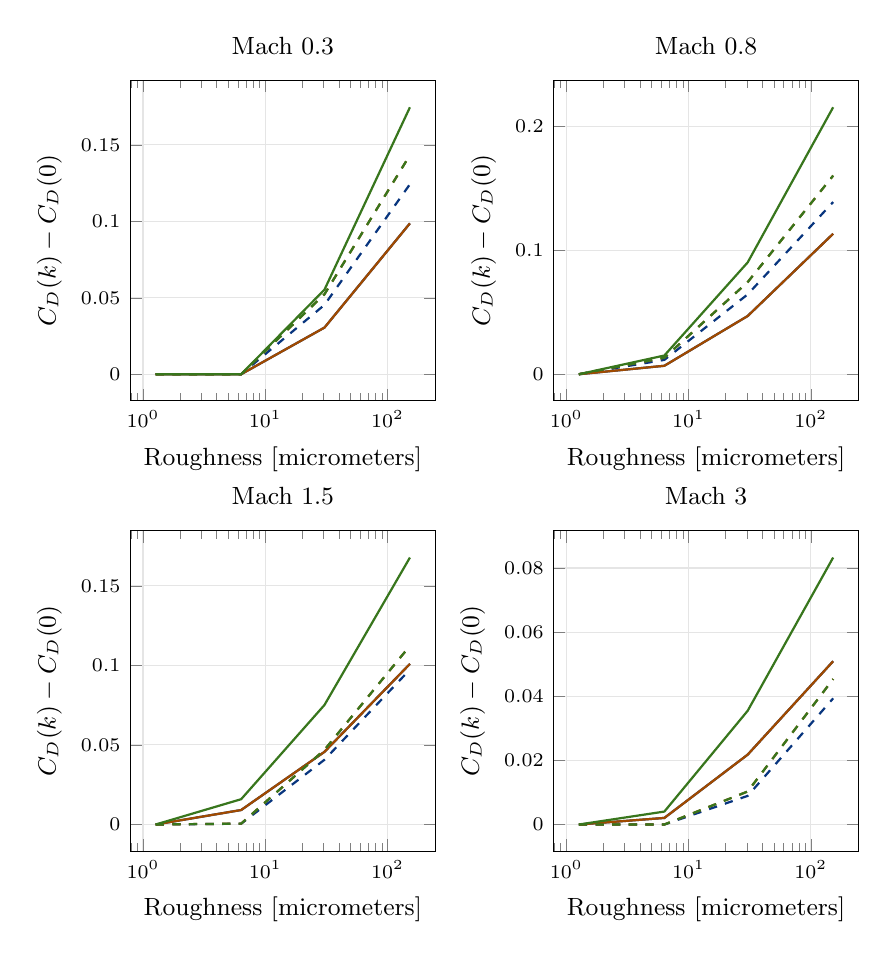
\begin{tikzpicture}
\begin{groupplot}[group style={group size=2 by 2,horizontal sep=1.50cm,vertical sep=1.65cm},width=.45\textwidth,height=5.65cm,grid=major,grid style={gray!20},tick label style={font=\scriptsize},label style={font=\small},title style={font=\small},scaled y ticks=false,yticklabel style={/pgf/number format/fixed,/pgf/number format/precision=3},unbounded coords=jump]
\nextgroupplot[title={Mach 0.3},xlabel={Roughness [micrometers]},ylabel={$C_D(k)-C_D(0)$},xmode=log]
\addplot[thick,B,dashed] coordinates {(1.27,0) (6.35,0) (30.48,0.04534628) (152.4,0.1242859)};
\addplot[thick,B] coordinates {(1.27,0) (6.35,0) (30.48,0.0304968) (152.4,0.09870125)};
\addplot[thick,burntorange,dashed] coordinates {(1.27,0) (6.35,0) (30.48,0.05230064) (152.4,0.1433465)};
\addplot[thick,burntorange] coordinates {(1.27,0) (6.35,0) (30.48,0.0304968) (152.4,0.09870125)};
\addplot[thick,g,dashed] coordinates {(1.27,0) (6.35,0) (30.48,0.05230064) (152.4,0.1433465)};
\addplot[thick,g] coordinates {(1.27,0) (6.35,0) (30.48,0.05529577) (152.4,0.174618)};
\nextgroupplot[title={Mach 0.8},xlabel={Roughness [micrometers]},ylabel={$C_D(k)-C_D(0)$},xmode=log]
\addplot[thick,B,dashed] coordinates {(1.27,0) (6.35,0.01158352) (30.48,0.06445536) (152.4,0.1390138)};
\addplot[thick,B] coordinates {(1.27,0) (6.35,0.006821197) (30.48,0.04700307) (152.4,0.1133965)};
\addplot[thick,burntorange,dashed] coordinates {(1.27,0) (6.35,0.01335998) (30.48,0.07434031) (152.4,0.1603331)};
\addplot[thick,burntorange] coordinates {(1.27,0) (6.35,0.006821197) (30.48,0.04700307) (152.4,0.1133965)};
\addplot[thick,g,dashed] coordinates {(1.27,0) (6.35,0.01335998) (30.48,0.07434031) (152.4,0.1603331)};
\addplot[thick,g] coordinates {(1.27,0) (6.35,0.01511551) (30.48,0.09026383) (152.4,0.2155161)};
\nextgroupplot[title={Mach 1.5},xlabel={Roughness [micrometers]},ylabel={$C_D(k)-C_D(0)$},xmode=log]
\addplot[thick,B,dashed] coordinates {(1.27,0) (6.35,0.0004777276) (30.48,0.04068201) (152.4,0.09737702)};
\addplot[thick,B] coordinates {(1.27,0) (6.35,0.009098526) (30.48,0.04566597) (152.4,0.1009449)};
\addplot[thick,burntorange,dashed] coordinates {(1.27,0) (6.35,0.0005509924) (30.48,0.04692105) (152.4,0.1123109)};
\addplot[thick,burntorange] coordinates {(1.27,0) (6.35,0.009098526) (30.48,0.04566597) (152.4,0.1009449)};
\addplot[thick,g,dashed] coordinates {(1.27,0) (6.35,0.0005509924) (30.48,0.04692105) (152.4,0.1123109)};
\addplot[thick,g] coordinates {(1.27,0) (6.35,0.01589666) (30.48,0.07511029) (152.4,0.1677869)};
\nextgroupplot[title={Mach 3},xlabel={Roughness [micrometers]},ylabel={$C_D(k)-C_D(0)$},xmode=log]
\addplot[thick,B,dashed] coordinates {(1.27,0) (6.35,0) (30.48,0.008926964) (152.4,0.0393302)};
\addplot[thick,B] coordinates {(1.27,0) (6.35,0.002050639) (30.48,0.0217857) (152.4,0.05091928)};
\addplot[thick,burntorange,dashed] coordinates {(1.27,0) (6.35,0) (30.48,0.01029601) (152.4,0.04536192)};
\addplot[thick,burntorange] coordinates {(1.27,0) (6.35,0.002050639) (30.48,0.0217857) (152.4,0.05091928)};
\addplot[thick,g,dashed] coordinates {(1.27,0) (6.35,0) (30.48,0.01029601) (152.4,0.04536192)};
\addplot[thick,g] coordinates {(1.27,0) (6.35,0.004036774) (30.48,0.03546998) (152.4,0.08325009)};
\end{groupplot}\end{tikzpicture}
\caption{Numerical physical roughness is matched in the reconstructed OR correlation. Pressure and base terms retain their native OR values.}\label{fig:atlas-18-roughness-increment}
\end{figure}
\noindent{\footnotesize Export files: \code{18-roughness-increment.svg} and \code{18-roughness-increment.png}.\\ Directory: \code{aerodynamic-investigation/extended/figures/}.}

\clearpage\subsubsection*{Isolated fin response to physical roughness}
\begin{figure}[H]\centering
{\footnotesize\begin{tabular}{lll}
\tikz[baseline=-.5ex]{\draw[thick,B,dashed] (0,0)--(.40,0);}\ Hsq OR exact k & \tikz[baseline=-.5ex]{\draw[thick,B] (0,0)--(.40,0);}\ Hsq RAS & \tikz[baseline=-.5ex]{\draw[thick,burntorange,dashed] (0,0)--(.40,0);}\ Hbev OR exact k\\
\tikz[baseline=-.5ex]{\draw[thick,burntorange] (0,0)--(.40,0);}\ Hbev RAS\\
\end{tabular}}\par\vspace{.7em}
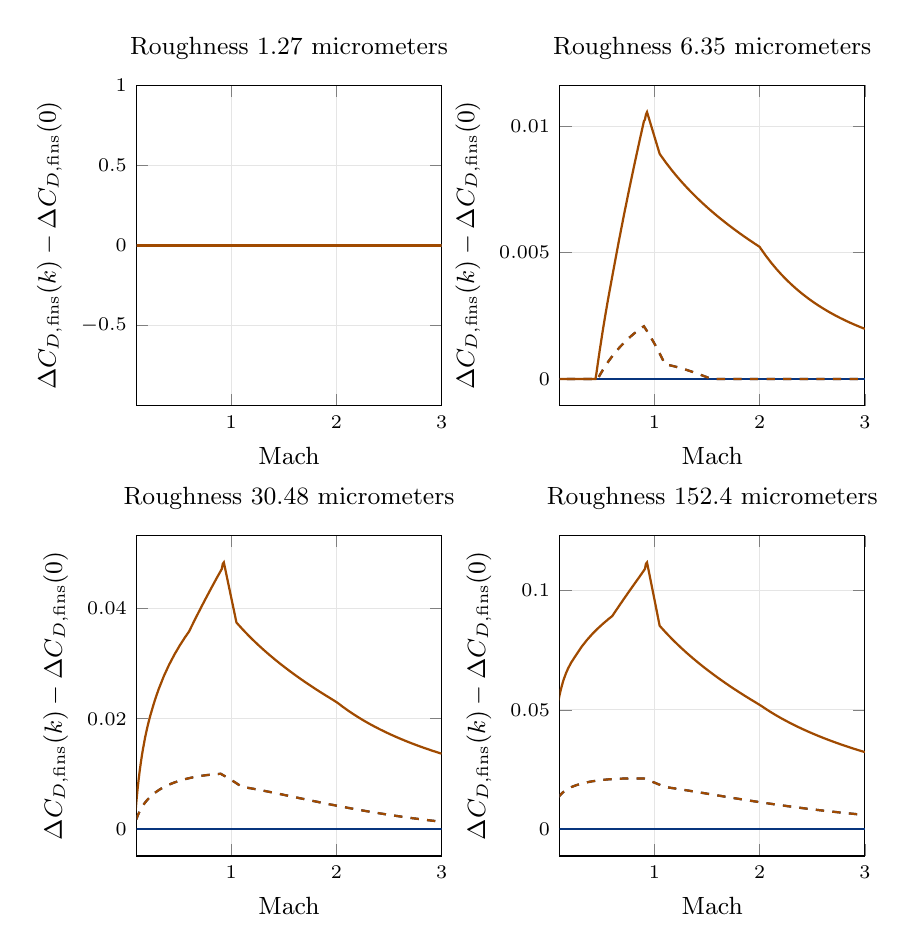
\begin{tikzpicture}
\begin{groupplot}[group style={group size=2 by 2,horizontal sep=1.50cm,vertical sep=1.65cm},width=.45\textwidth,height=5.65cm,grid=major,grid style={gray!20},tick label style={font=\scriptsize},label style={font=\small},title style={font=\small},scaled y ticks=false,yticklabel style={/pgf/number format/fixed,/pgf/number format/precision=3},unbounded coords=jump]
\nextgroupplot[title={Roughness 1.27 micrometers},xlabel={Mach},ylabel={$\Delta C_{D,\mathrm{fins}}(k)-\Delta C_{D,\mathrm{fins}}(0)$},xmin=0.1,xmax=3]
\addplot[thick,B,dashed] coordinates {(0.01,0) (0.06,0) (0.11,0) (0.16,0) (0.21,0) (0.26,0) (0.31,0) (0.36,0) (0.41,0) (0.46,0) (0.51,0) (0.56,0) (0.61,0) (0.66,0) (0.71,0) (0.76,0) (0.81,0) (0.86,0) (0.91,0) (0.96,0) (1.01,0) (1.06,0) (1.11,0) (1.16,0) (1.21,0) (1.26,0) (1.31,0) (1.36,0) (1.41,0) (1.46,0) (1.51,0) (1.56,0) (1.61,0) (1.66,0) (1.71,0) (1.76,0) (1.81,0) (1.86,0) (1.91,0) (1.96,0) (2.01,0) (2.06,0) (2.11,0) (2.16,0) (2.21,0) (2.26,0) (2.31,0) (2.36,0) (2.41,0) (2.46,0) (2.51,0) (2.56,0) (2.61,0) (2.66,0) (2.71,0) (2.76,0) (2.81,0) (2.86,0) (2.91,0) (2.96,0) (3,0)};
\addplot[thick,B] coordinates {(0.01,0) (0.06,0) (0.11,0) (0.16,0) (0.21,0) (0.26,0) (0.31,0) (0.36,0) (0.41,0) (0.46,0) (0.51,0) (0.56,0) (0.61,0) (0.66,0) (0.71,0) (0.76,0) (0.81,0) (0.86,0) (0.91,0) (0.96,0) (1.01,0) (1.06,0) (1.11,0) (1.16,0) (1.21,0) (1.26,0) (1.31,0) (1.36,0) (1.41,0) (1.46,0) (1.51,0) (1.56,0) (1.61,0) (1.66,0) (1.71,0) (1.76,0) (1.81,0) (1.86,0) (1.91,0) (1.96,0) (2.01,0) (2.06,0) (2.11,0) (2.16,0) (2.21,0) (2.26,0) (2.31,0) (2.36,0) (2.41,0) (2.46,0) (2.51,0) (2.56,0) (2.61,0) (2.66,0) (2.71,0) (2.76,0) (2.81,0) (2.86,0) (2.91,0) (2.96,0) (3,0)};
\addplot[thick,burntorange,dashed] coordinates {(0.01,0) (0.06,0) (0.11,0) (0.16,0) (0.21,0) (0.26,0) (0.31,0) (0.36,0) (0.41,0) (0.46,0) (0.51,0) (0.56,0) (0.61,0) (0.66,0) (0.71,0) (0.76,0) (0.81,0) (0.86,0) (0.91,0) (0.96,0) (1.01,0) (1.06,0) (1.11,0) (1.16,0) (1.21,0) (1.26,0) (1.31,0) (1.36,0) (1.41,0) (1.46,0) (1.51,0) (1.56,0) (1.61,0) (1.66,0) (1.71,0) (1.76,0) (1.81,0) (1.86,0) (1.91,0) (1.96,0) (2.01,0) (2.06,0) (2.11,0) (2.16,0) (2.21,0) (2.26,0) (2.31,0) (2.36,0) (2.41,0) (2.46,0) (2.51,0) (2.56,0) (2.61,0) (2.66,0) (2.71,0) (2.76,0) (2.81,0) (2.86,0) (2.91,0) (2.96,0) (3,0)};
\addplot[thick,burntorange] coordinates {(0.01,0) (0.06,0) (0.11,0) (0.16,0) (0.21,0) (0.26,0) (0.31,0) (0.36,0) (0.41,0) (0.46,0) (0.51,0) (0.56,0) (0.61,0) (0.66,0) (0.71,0) (0.76,0) (0.81,0) (0.86,0) (0.91,0) (0.96,0) (1.01,0) (1.06,0) (1.11,0) (1.16,0) (1.21,0) (1.26,0) (1.31,0) (1.36,0) (1.41,0) (1.46,0) (1.51,0) (1.56,0) (1.61,0) (1.66,0) (1.71,0) (1.76,0) (1.81,0) (1.86,0) (1.91,0) (1.96,0) (2.01,0) (2.06,0) (2.11,0) (2.16,0) (2.21,0) (2.26,0) (2.31,0) (2.36,0) (2.41,0) (2.46,0) (2.51,0) (2.56,0) (2.61,0) (2.66,0) (2.71,0) (2.76,0) (2.81,0) (2.86,0) (2.91,0) (2.96,0) (3,0)};
\nextgroupplot[title={Roughness 6.35 micrometers},xlabel={Mach},ylabel={$\Delta C_{D,\mathrm{fins}}(k)-\Delta C_{D,\mathrm{fins}}(0)$},xmin=0.1,xmax=3]
\addplot[thick,B,dashed] coordinates {(0.01,0) (0.06,0) (0.11,0) (0.16,0) (0.21,0) (0.26,0) (0.31,0) (0.36,0) (0.41,0) (0.46,0) (0.49,0.000222324) (0.51,0.0003615712) (0.53,0.000493629) (0.56,0.0006794268) (0.58,0.0007957906) (0.61,0.0009601075) (0.63,0.001063351) (0.66,0.001209539) (0.68,0.00130161) (0.71,0.001432236) (0.73,0.001514643) (0.76,0.001631712) (0.78,0.001705643) (0.81,0.001810745) (0.86,0.00197157) (0.9,0.002088353) (0.91,0.00202536) (0.94,0.001829436) (0.96,0.001692831) (0.99,0.001478495) (1.01,0.001329039) (1.04,0.001094488) (1.06,0.0009308891) (1.08,0.0007612331) (1.1,0.0005852766) (1.11,0.0005774221) (1.16,0.000532886) (1.21,0.0004804802) (1.26,0.0004213395) (1.31,0.0003564891) (1.36,0.000286856) (1.41,0.0002132781) (1.46,0.0001365121) (1.51,5.724041e-05) (1.54,8.7328e-06) (1.55,0) (1.56,0) (1.61,0) (1.66,0) (1.71,0) (1.76,0) (1.81,0) (1.86,0) (1.91,0) (1.96,0) (2.01,0) (2.06,0) (2.11,0) (2.16,0) (2.21,0) (2.26,0) (2.31,0) (2.36,0) (2.41,0) (2.46,0) (2.51,0) (2.56,0) (2.61,0) (2.66,0) (2.71,0) (2.76,0) (2.81,0) (2.86,0) (2.91,0) (2.96,0) (3,0)};
\addplot[thick,B] coordinates {(0.01,0) (0.06,0) (0.11,0) (0.16,0) (0.21,0) (0.26,0) (0.31,0) (0.36,0) (0.41,0) (0.46,0) (0.51,0) (0.56,5.551115e-17) (0.61,-8.326673e-17) (0.66,8.326673e-17) (0.71,5.551115e-17) (0.76,5.551115e-17) (0.81,-5.551115e-17) (0.86,0) (0.91,-2.775558e-17) (0.95,1.054712e-15) (0.96,9.992007e-16) (0.98,-1.054712e-15) (1.01,-9.992007e-16) (1.06,0) (1.11,-5.551115e-17) (1.16,0) (1.21,0) (1.26,0) (1.31,-5.551115e-17) (1.36,5.551115e-17) (1.41,1.110223e-16) (1.46,5.551115e-17) (1.51,0) (1.56,0) (1.61,-5.551115e-17) (1.66,-1.110223e-16) (1.71,0) (1.76,5.551115e-17) (1.81,5.551115e-17) (1.86,0) (1.91,-5.551115e-17) (1.96,5.551115e-17) (2.01,-5.551115e-17) (2.06,-5.551115e-17) (2.11,0) (2.16,5.551115e-17) (2.21,5.551115e-17) (2.26,5.551115e-17) (2.31,0) (2.36,-1.110223e-16) (2.41,-5.551115e-17) (2.46,-5.551115e-17) (2.51,-5.551115e-17) (2.56,0) (2.61,5.551115e-17) (2.66,5.551115e-17) (2.71,5.551115e-17) (2.76,0) (2.81,0) (2.86,5.551115e-17) (2.91,5.551115e-17) (2.96,-5.551115e-17) (3,5.551115e-17)};
\addplot[thick,burntorange,dashed] coordinates {(0.01,0) (0.06,0) (0.11,0) (0.16,0) (0.21,0) (0.26,0) (0.31,0) (0.36,0) (0.41,0) (0.46,0) (0.49,0.000222324) (0.51,0.0003615712) (0.53,0.000493629) (0.56,0.0006794268) (0.58,0.0007957906) (0.61,0.0009601075) (0.63,0.001063351) (0.66,0.001209539) (0.68,0.00130161) (0.71,0.001432236) (0.73,0.001514643) (0.76,0.001631712) (0.78,0.001705643) (0.81,0.001810745) (0.86,0.00197157) (0.9,0.002088353) (0.91,0.00202536) (0.94,0.001829436) (0.96,0.001692831) (0.99,0.001478495) (1.01,0.001329039) (1.04,0.001094488) (1.06,0.0009308891) (1.08,0.0007612331) (1.1,0.0005852766) (1.11,0.0005774221) (1.16,0.000532886) (1.21,0.0004804802) (1.26,0.0004213395) (1.31,0.0003564891) (1.36,0.000286856) (1.41,0.0002132781) (1.46,0.0001365121) (1.51,5.724041e-05) (1.54,8.7328e-06) (1.55,0) (1.56,0) (1.61,0) (1.66,0) (1.71,0) (1.76,0) (1.81,0) (1.86,0) (1.91,0) (1.96,0) (2.01,0) (2.06,0) (2.11,0) (2.16,0) (2.21,0) (2.26,0) (2.31,0) (2.36,0) (2.41,0) (2.46,0) (2.51,0) (2.56,0) (2.61,0) (2.66,0) (2.71,0) (2.76,0) (2.81,0) (2.86,0) (2.91,0) (2.96,0) (3,0)};
\addplot[thick,burntorange] coordinates {(0.01,0) (0.06,0) (0.11,0) (0.16,0) (0.21,0) (0.26,0) (0.31,0) (0.36,0) (0.41,0) (0.44,0) (0.45,0.000259258) (0.46,0.0005562229) (0.48,0.001128141) (0.51,0.001936165) (0.53,0.002445091) (0.56,0.003168787) (0.61,0.004298914) (0.66,0.005413641) (0.71,0.006478409) (0.76,0.007501499) (0.81,0.008489333) (0.86,0.009447107) (0.9,0.01019446) (0.91,0.01026378) (0.92,0.01047175) (0.93,0.01055894) (0.96,0.01014623) (1.01,0.009458385) (1.05,0.008908106) (1.06,0.008847835) (1.11,0.008558829) (1.16,0.008288411) (1.21,0.008034261) (1.26,0.00779444) (1.31,0.007567325) (1.36,0.007351533) (1.41,0.007145884) (1.46,0.006949368) (1.51,0.006761107) (1.56,0.006580338) (1.61,0.006406398) (1.66,0.006238699) (1.71,0.006076726) (1.76,0.005920022) (1.81,0.005768179) (1.86,0.005620834) (1.91,0.005477659) (1.96,0.005338365) (2,0.005229543) (2.01,0.005167566) (2.06,0.004872585) (2.11,0.004601747) (2.16,0.004352349) (2.21,0.004122082) (2.26,0.003908953) (2.31,0.003711246) (2.36,0.003527457) (2.41,0.003356275) (2.46,0.003196548) (2.51,0.003047256) (2.56,0.002907499) (2.61,0.002776472) (2.66,0.002653461) (2.71,0.002537821) (2.76,0.002428977) (2.81,0.002326409) (2.86,0.002229648) (2.91,0.002138269) (2.96,0.002051886) (3,0.001986135)};
\nextgroupplot[title={Roughness 30.48 micrometers},xlabel={Mach},ylabel={$\Delta C_{D,\mathrm{fins}}(k)-\Delta C_{D,\mathrm{fins}}(0)$},xmin=0.1,xmax=3]
\addplot[thick,B,dashed] coordinates {(0.01,0) (0.06,0) (0.07,0) (0.08,0.0006783682) (0.09,0.001334757) (0.1,0.001904404) (0.11,0.00240592) (0.12,0.002852641) (0.13,0.003254422) (0.14,0.003618738) (0.15,0.003951382) (0.16,0.004256931) (0.17,0.004539053) (0.18,0.004800736) (0.19,0.005044441) (0.21,0.005485783) (0.23,0.005875932) (0.26,0.006385008) (0.28,0.006683257) (0.31,0.007080928) (0.33,0.007318118) (0.36,0.007638864) (0.38,0.007832446) (0.41,0.008096687) (0.46,0.008478174) (0.51,0.008799157) (0.56,0.009070666) (0.61,0.009300668) (0.66,0.00949509) (0.71,0.009658447) (0.76,0.00979425) (0.81,0.00990528) (0.86,0.009993769) (0.9,0.01004957) (0.91,0.00994419) (0.96,0.009399751) (1.01,0.008824049) (1.06,0.008213989) (1.1,0.007698848) (1.11,0.007667833) (1.16,0.007506684) (1.21,0.007336552) (1.26,0.007158875) (1.31,0.006974963) (1.36,0.006786013) (1.41,0.006593111) (1.46,0.00639725) (1.51,0.006199326) (1.56,0.006000151) (1.61,0.005800459) (1.66,0.005600907) (1.71,0.005402085) (1.76,0.005204518) (1.81,0.00500867) (1.86,0.004814953) (1.91,0.004623725) (1.96,0.004435299) (2.01,0.004249944) (2.06,0.00406789) (2.11,0.00388933) (2.16,0.003714425) (2.21,0.003543306) (2.26,0.003376075) (2.31,0.003212812) (2.36,0.003053575) (2.41,0.002898399) (2.46,0.002747304) (2.51,0.002600295) (2.56,0.002457361) (2.61,0.00231848) (2.66,0.002183619) (2.71,0.002052734) (2.76,0.001925776) (2.81,0.001802687) (2.86,0.001683402) (2.91,0.001567854) (2.96,0.001455969) (3,0.001369048)};
\addplot[thick,B] coordinates {(0.01,0) (0.06,0) (0.11,-1.110223e-16) (0.16,5.551115e-17) (0.21,0) (0.26,-8.326673e-17) (0.31,0) (0.36,8.326673e-17) (0.41,0) (0.46,-8.326673e-17) (0.51,2.775558e-17) (0.56,-2.775558e-17) (0.61,-2.775558e-17) (0.66,5.551115e-17) (0.71,2.775558e-17) (0.76,5.551115e-17) (0.81,0) (0.86,0) (0.91,2.775558e-17) (0.95,2.053913e-15) (0.96,9.436896e-16) (1.01,-1.110223e-15) (1.06,5.551115e-17) (1.11,0) (1.16,0) (1.21,1.110223e-16) (1.26,-1.110223e-16) (1.31,0) (1.36,0) (1.41,0) (1.46,0) (1.51,-5.551115e-17) (1.56,5.551115e-17) (1.61,-5.551115e-17) (1.66,0) (1.71,0) (1.76,5.551115e-17) (1.81,5.551115e-17) (1.86,0) (1.91,0) (1.96,5.551115e-17) (2.01,-5.551115e-17) (2.06,-5.551115e-17) (2.11,0) (2.16,5.551115e-17) (2.21,0) (2.26,5.551115e-17) (2.31,0) (2.36,-5.551115e-17) (2.41,0) (2.46,0) (2.51,-5.551115e-17) (2.56,5.551115e-17) (2.61,-5.551115e-17) (2.66,5.551115e-17) (2.71,-5.551115e-17) (2.76,0) (2.81,0) (2.86,5.551115e-17) (2.91,0) (2.96,0) (3,5.551115e-17)};
\addplot[thick,burntorange,dashed] coordinates {(0.01,0) (0.06,0) (0.07,0) (0.08,0.0006783682) (0.09,0.001334757) (0.1,0.001904404) (0.11,0.00240592) (0.12,0.002852641) (0.13,0.003254422) (0.14,0.003618738) (0.15,0.003951382) (0.16,0.004256931) (0.17,0.004539053) (0.18,0.004800736) (0.19,0.005044441) (0.21,0.005485783) (0.23,0.005875932) (0.26,0.006385008) (0.28,0.006683257) (0.31,0.007080928) (0.33,0.007318118) (0.36,0.007638864) (0.38,0.007832446) (0.41,0.008096687) (0.46,0.008478174) (0.51,0.008799157) (0.56,0.009070666) (0.61,0.009300668) (0.66,0.00949509) (0.71,0.009658447) (0.76,0.00979425) (0.81,0.00990528) (0.86,0.009993769) (0.9,0.01004957) (0.91,0.00994419) (0.96,0.009399751) (1.01,0.008824049) (1.06,0.008213989) (1.1,0.007698848) (1.11,0.007667833) (1.16,0.007506684) (1.21,0.007336552) (1.26,0.007158875) (1.31,0.006974963) (1.36,0.006786013) (1.41,0.006593111) (1.46,0.00639725) (1.51,0.006199326) (1.56,0.006000151) (1.61,0.005800459) (1.66,0.005600907) (1.71,0.005402085) (1.76,0.005204518) (1.81,0.00500867) (1.86,0.004814953) (1.91,0.004623725) (1.96,0.004435299) (2.01,0.004249944) (2.06,0.00406789) (2.11,0.00388933) (2.16,0.003714425) (2.21,0.003543306) (2.26,0.003376075) (2.31,0.003212812) (2.36,0.003053575) (2.41,0.002898399) (2.46,0.002747304) (2.51,0.002600295) (2.56,0.002457361) (2.61,0.00231848) (2.66,0.002183619) (2.71,0.002052734) (2.76,0.001925776) (2.81,0.001802687) (2.86,0.001683402) (2.91,0.001567854) (2.96,0.001455969) (3,0.001369048)};
\addplot[thick,burntorange] coordinates {(0.01,0) (0.06,0) (0.07,0) (0.08,0.000441835) (0.09,0.003031543) (0.1,0.005267778) (0.11,0.007227264) (0.12,0.008964904) (0.13,0.01052117) (0.14,0.01192669) (0.15,0.0132052) (0.16,0.01437535) (0.18,0.01644771) (0.19,0.01737211) (0.21,0.01903925) (0.23,0.02050572) (0.26,0.02245908) (0.28,0.02367643) (0.31,0.02532917) (0.36,0.02772477) (0.41,0.02978633) (0.46,0.03160147) (0.51,0.03322825) (0.56,0.03470703) (0.6,0.03580323) (0.61,0.03620056) (0.66,0.03812659) (0.71,0.03999923) (0.76,0.04182677) (0.81,0.04361573) (0.86,0.04537132) (0.91,0.04707253) (0.92,0.04802633) (0.93,0.04828849) (0.96,0.04556939) (1.01,0.04103757) (1.05,0.03741211) (1.06,0.03719523) (1.11,0.03614652) (1.16,0.03515207) (1.21,0.0342058) (1.26,0.03330255) (1.31,0.03243794) (1.36,0.0316082) (1.41,0.03081007) (1.46,0.03004074) (1.51,0.02929771) (1.56,0.02857882) (1.61,0.02788214) (1.66,0.02720596) (1.71,0.02654877) (1.76,0.02590921) (1.81,0.02528606) (1.86,0.02467821) (1.91,0.02408467) (1.96,0.02350454) (2.01,0.02289971) (2.06,0.02217505) (2.11,0.02149435) (2.16,0.02085315) (2.21,0.02024766) (2.26,0.01967457) (2.31,0.01913103) (2.36,0.01861454) (2.41,0.01812291) (2.46,0.0176542) (2.51,0.01720669) (2.56,0.01677884) (2.61,0.01636928) (2.66,0.01597679) (2.71,0.01560024) (2.76,0.01523863) (2.81,0.01489105) (2.86,0.01455666) (2.91,0.01423469) (2.96,0.01392446) (3,0.01368428)};
\nextgroupplot[title={Roughness 152.4 micrometers},xlabel={Mach},ylabel={$\Delta C_{D,\mathrm{fins}}(k)-\Delta C_{D,\mathrm{fins}}(0)$},xmin=0.1,xmax=3]
\addplot[thick,B,dashed] coordinates {(0.01,0) (0.02,0.003279222) (0.03,0.006502754) (0.04,0.008564802) (0.05,0.01004986) (0.06,0.01119506) (0.07,0.01211845) (0.08,0.01288675) (0.09,0.01354106) (0.1,0.01410839) (0.11,0.01460734) (0.12,0.01505125) (0.13,0.01544998) (0.14,0.015811) (0.16,0.01644186) (0.18,0.01697736) (0.21,0.01764811) (0.23,0.01802751) (0.26,0.01851863) (0.31,0.01917973) (0.36,0.01969674) (0.41,0.02010753) (0.46,0.02043588) (0.51,0.02069761) (0.56,0.02090377) (0.61,0.0210623) (0.66,0.02117915) (0.71,0.02125883) (0.76,0.02130484) (0.81,0.02131998) (0.86,0.02130646) (0.9,0.02127625) (0.91,0.02111111) (0.96,0.02026784) (1.01,0.01939331) (1.06,0.01848442) (1.1,0.01773022) (1.11,0.01766654) (1.16,0.01734095) (1.21,0.0170048) (1.26,0.01665997) (1.31,0.01630816) (1.36,0.01595095) (1.41,0.01558978) (1.46,0.01522598) (1.51,0.01486073) (1.56,0.01449514) (1.61,0.01413019) (1.66,0.01376677) (1.71,0.01340569) (1.76,0.01304764) (1.81,0.01269327) (1.86,0.01234314) (1.91,0.01199773) (1.96,0.01165746) (2.01,0.01132271) (2.06,0.01099377) (2.11,0.01067092) (2.16,0.01035436) (2.21,0.01004427) (2.26,0.009740775) (2.31,0.009443985) (2.36,0.009153964) (2.41,0.008870754) (2.46,0.008594369) (2.51,0.008324802) (2.56,0.008062028) (2.61,0.007806002) (2.66,0.007556665) (2.71,0.007313943) (2.76,0.007077752) (2.81,0.006847997) (2.86,0.006624575) (2.91,0.006407375) (2.96,0.006196281) (3,0.006031721)};
\addplot[thick,B] coordinates {(0.01,0) (0.06,0) (0.11,0) (0.16,5.551115e-17) (0.21,0) (0.26,-2.775558e-17) (0.31,-5.551115e-17) (0.36,-2.775558e-17) (0.41,0) (0.46,2.775558e-17) (0.51,2.775558e-17) (0.56,2.775558e-17) (0.61,-2.775558e-17) (0.66,5.551115e-17) (0.71,2.775558e-17) (0.76,5.551115e-17) (0.81,0) (0.86,5.551115e-17) (0.91,2.775558e-17) (0.92,9.436896e-16) (0.96,9.436896e-16) (0.98,-1.054712e-15) (1.01,-9.992007e-16) (1.06,5.551115e-17) (1.11,-1.110223e-16) (1.16,0) (1.21,5.551115e-17) (1.26,-5.551115e-17) (1.31,-5.551115e-17) (1.36,1.110223e-16) (1.41,0) (1.46,0) (1.51,-5.551115e-17) (1.56,5.551115e-17) (1.61,-5.551115e-17) (1.66,-1.110223e-16) (1.71,0) (1.76,5.551115e-17) (1.81,5.551115e-17) (1.86,0) (1.91,-1.110223e-16) (1.96,1.110223e-16) (2.01,-5.551115e-17) (2.06,-5.551115e-17) (2.11,-5.551115e-17) (2.16,5.551115e-17) (2.21,0) (2.26,0) (2.31,0) (2.36,0) (2.41,0) (2.46,-5.551115e-17) (2.51,0) (2.56,0) (2.61,5.551115e-17) (2.66,5.551115e-17) (2.71,5.551115e-17) (2.76,5.551115e-17) (2.81,0) (2.86,5.551115e-17) (2.91,0) (2.96,-5.551115e-17) (3,5.551115e-17)};
\addplot[thick,burntorange,dashed] coordinates {(0.01,0) (0.02,0.003279222) (0.03,0.006502754) (0.04,0.008564802) (0.05,0.01004986) (0.06,0.01119506) (0.07,0.01211845) (0.08,0.01288675) (0.09,0.01354106) (0.1,0.01410839) (0.11,0.01460734) (0.12,0.01505125) (0.13,0.01544998) (0.14,0.015811) (0.16,0.01644186) (0.18,0.01697736) (0.21,0.01764811) (0.23,0.01802751) (0.26,0.01851863) (0.31,0.01917973) (0.36,0.01969674) (0.41,0.02010753) (0.46,0.02043588) (0.51,0.02069761) (0.56,0.02090377) (0.61,0.0210623) (0.66,0.02117915) (0.71,0.02125883) (0.76,0.02130484) (0.81,0.02131998) (0.86,0.02130646) (0.9,0.02127625) (0.91,0.02111111) (0.96,0.02026784) (1.01,0.01939331) (1.06,0.01848442) (1.1,0.01773022) (1.11,0.01766654) (1.16,0.01734095) (1.21,0.0170048) (1.26,0.01665997) (1.31,0.01630816) (1.36,0.01595095) (1.41,0.01558978) (1.46,0.01522598) (1.51,0.01486073) (1.56,0.01449514) (1.61,0.01413019) (1.66,0.01376677) (1.71,0.01340569) (1.76,0.01304764) (1.81,0.01269327) (1.86,0.01234314) (1.91,0.01199773) (1.96,0.01165746) (2.01,0.01132271) (2.06,0.01099377) (2.11,0.01067092) (2.16,0.01035436) (2.21,0.01004427) (2.26,0.009740775) (2.31,0.009443985) (2.36,0.009153964) (2.41,0.008870754) (2.46,0.008594369) (2.51,0.008324802) (2.56,0.008062028) (2.61,0.007806002) (2.66,0.007556665) (2.71,0.007313943) (2.76,0.007077752) (2.81,0.006847997) (2.86,0.006624575) (2.91,0.006407375) (2.96,0.006196281) (3,0.006031721)};
\addplot[thick,burntorange] coordinates {(0.01,0) (0.02,0.0128487) (0.03,0.02610536) (0.04,0.03448616) (0.05,0.04046356) (0.06,0.04503409) (0.07,0.04869121) (0.08,0.05171268) (0.09,0.05426905) (0.1,0.05647203) (0.11,0.05839836) (0.13,0.06162621) (0.14,0.06299886) (0.16,0.06538204) (0.18,0.06738928) (0.21,0.06988383) (0.26,0.07325596) (0.31,0.07652705) (0.36,0.07932234) (0.41,0.08178234) (0.46,0.08399464) (0.51,0.08601735) (0.56,0.08789087) (0.6,0.08930197) (0.61,0.08997659) (0.66,0.09324939) (0.71,0.09646218) (0.76,0.09962338) (0.81,0.1027396) (0.86,0.1058161) (0.91,0.1089878) (0.92,0.1111962) (0.93,0.111747) (0.96,0.1051144) (1.01,0.09406015) (1.05,0.08521672) (1.06,0.08471667) (1.11,0.08229814) (1.16,0.08000426) (1.21,0.07782131) (1.26,0.07573763) (1.31,0.0737433) (1.36,0.07182974) (1.41,0.06998956) (1.46,0.06821627) (1.51,0.06650424) (1.56,0.06484845) (1.61,0.06324451) (1.66,0.06168849) (1.71,0.06017688) (1.76,0.05870655) (1.81,0.05727468) (1.86,0.05587872) (1.91,0.05451636) (1.96,0.05318551) (2.01,0.05183848) (2.06,0.05036309) (2.11,0.04896901) (2.16,0.04764834) (2.21,0.04639432) (2.26,0.0452011) (2.31,0.04406359) (2.36,0.04297736) (2.41,0.04193848) (2.46,0.04094348) (2.51,0.03998929) (2.56,0.03907316) (2.61,0.03819261) (2.66,0.03734541) (2.71,0.03652955) (2.76,0.0357432) (2.81,0.03498469) (2.86,0.03425249) (2.91,0.03354521) (2.96,0.03286154) (3,0.03233081)};
\end{groupplot}\end{tikzpicture}
\caption{Two subtractions remove smooth baseline drag and the finless-body roughness response. RASAero square-fin curves remain at zero to floating-point precision; beveled fins respond. OR exact-roughness curves are reconstructed from its native correlation.}\label{fig:atlas-27-fin-roughness-response}
\end{figure}
\noindent{\footnotesize Export files: \code{27-fin-roughness-response.svg} and \code{27-fin-roughness-response.png}.\\ Directory: \code{aerodynamic-investigation/extended/figures/}.}

\clearpage\subsubsection*{Laminar-to-turbulent option: finned rockets}
\begin{figure}[H]\centering
{\footnotesize\begin{tabular}{ll}
\tikz[baseline=-.5ex]{\draw[thick,B,dashed] (0,0)--(.40,0);}\ MIT OR & \tikz[baseline=-.5ex]{\draw[thick,burntorange] (0,0)--(.40,0);}\ RASAero\\
\end{tabular}}\par\vspace{.7em}
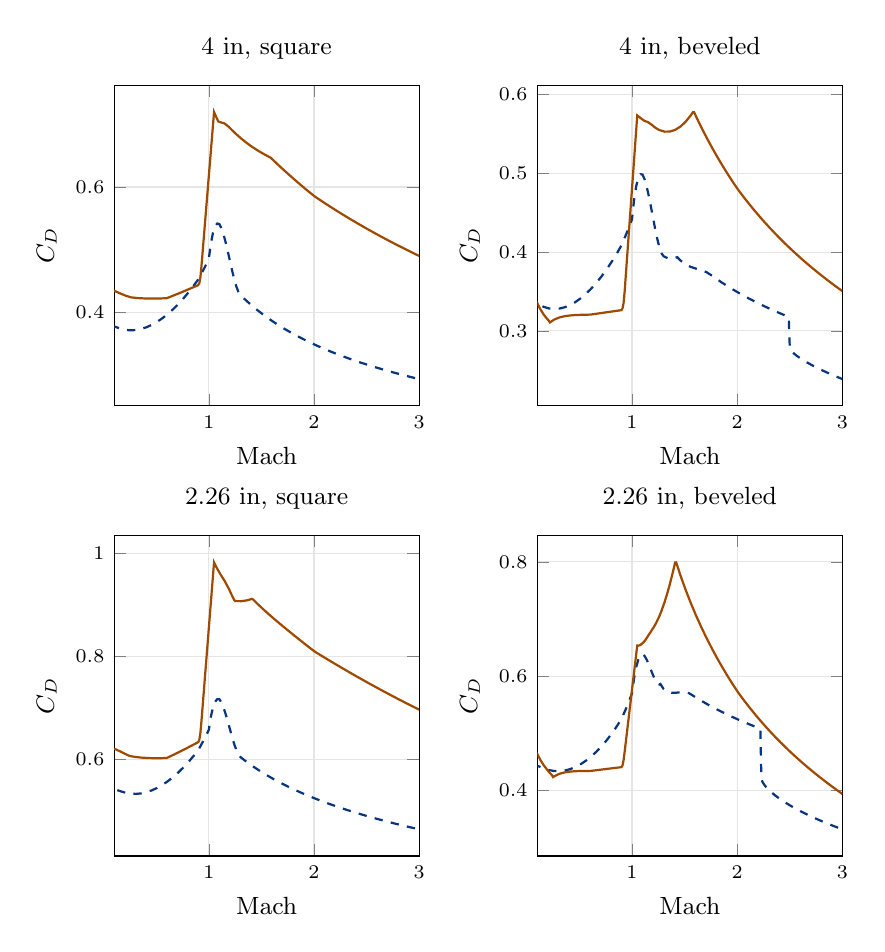
\begin{tikzpicture}
\begin{groupplot}[group style={group size=2 by 2,horizontal sep=1.50cm,vertical sep=1.65cm},width=.45\textwidth,height=5.65cm,grid=major,grid style={gray!20},tick label style={font=\scriptsize},label style={font=\small},title style={font=\small},scaled y ticks=false,yticklabel style={/pgf/number format/fixed,/pgf/number format/precision=3},unbounded coords=jump]
\nextgroupplot[title={4 in, square},xlabel={Mach},ylabel={$C_D$},xmin=0.1,xmax=3]
\addplot[thick,B,dashed] coordinates {(0.01,0.3284644) (0.02,0.3305305) (0.03,0.3595401) (0.04,0.3707199) (0.05,0.3756258) (0.06,0.3777902) (0.07,0.378602) (0.08,0.3786972) (0.11,0.3773409) (0.16,0.3743039) (0.21,0.3722982) (0.26,0.3716144) (0.31,0.3721871) (0.36,0.3739185) (0.41,0.3767262) (0.46,0.3805462) (0.51,0.38533) (0.56,0.3910408) (0.61,0.3976501) (0.66,0.4051362) (0.71,0.4134822) (0.76,0.4226748) (0.81,0.4327039) (0.86,0.4435616) (0.9,0.4528403) (0.91,0.4558166) (0.96,0.4715527) (1,0.485186) (1.01,0.4977807) (1.02,0.5101953) (1.04,0.5272594) (1.06,0.5375172) (1.08,0.5418466) (1.1,0.5411273) (1.11,0.5378148) (1.12,0.5345425) (1.14,0.5245567) (1.16,0.5120498) (1.18,0.4979028) (1.21,0.4755914) (1.22,0.4682154) (1.24,0.45444) (1.26,0.4425545) (1.28,0.4334427) (1.3,0.4279889) (1.31,0.4263364) (1.36,0.4184173) (1.41,0.4110252) (1.46,0.4041002) (1.51,0.3975938) (1.56,0.3914637) (1.61,0.3856742) (1.66,0.3801939) (1.71,0.3749957) (1.76,0.3700555) (1.81,0.3653524) (1.86,0.3608673) (1.91,0.3565837) (1.96,0.3524865) (2.01,0.3485622) (2.06,0.3447986) (2.11,0.3411847) (2.16,0.3377105) (2.21,0.334367) (2.26,0.3311458) (2.31,0.3280395) (2.36,0.3250409) (2.41,0.3221439) (2.46,0.3193424) (2.51,0.3166312) (2.56,0.3140052) (2.61,0.3114599) (2.66,0.3089909) (2.71,0.3065943) (2.76,0.3042664) (2.81,0.3020039) (2.86,0.2998035) (2.91,0.2976622) (2.96,0.2955774) (3,0.2939483)};
\addplot[thick,burntorange] coordinates {(0.01,0.3959172) (0.02,0.4021125) (0.03,0.4221951) (0.04,0.4302792) (0.05,0.433817) (0.06,0.4353099) (0.08,0.4356894) (0.11,0.4340484) (0.16,0.4303144) (0.21,0.4268548) (0.26,0.4242006) (0.31,0.4232653) (0.36,0.4226707) (0.41,0.4223492) (0.46,0.422249) (0.51,0.4223299) (0.56,0.4225613) (0.6,0.4228385) (0.61,0.4235061) (0.66,0.4268007) (0.71,0.4301878) (0.76,0.433655) (0.81,0.4371923) (0.86,0.4407912) (0.9,0.44371) (0.91,0.4467272) (0.92,0.4557789) (0.93,0.4728424) (0.96,0.5344907) (1.01,0.637238) (1.05,0.7194358) (1.06,0.715688) (1.09,0.7046404) (1.11,0.7034299) (1.15,0.7012885) (1.16,0.6999681) (1.19,0.6959758) (1.21,0.6925189) (1.26,0.6844354) (1.31,0.6770769) (1.36,0.6703781) (1.41,0.6642906) (1.46,0.6587769) (1.51,0.6538067) (1.56,0.6493562) (1.59,0.6465663) (1.61,0.6433003) (1.66,0.6353137) (1.71,0.6275536) (1.76,0.6199908) (1.81,0.6126013) (1.86,0.6053658) (1.91,0.5982681) (1.96,0.591295) (2.01,0.5846682) (2.06,0.5790447) (2.11,0.5735299) (2.16,0.5681193) (2.21,0.5628085) (2.26,0.5575946) (2.31,0.5524745) (2.36,0.5474459) (2.41,0.5425061) (2.46,0.5376532) (2.51,0.5328852) (2.56,0.5281997) (2.61,0.5235948) (2.66,0.5190683) (2.71,0.514618) (2.76,0.5102415) (2.81,0.5059364) (2.86,0.5017002) (2.91,0.4975302) (2.96,0.4934236) (3,0.4901821)};
\nextgroupplot[title={4 in, beveled},xlabel={Mach},ylabel={$C_D$},xmin=0.1,xmax=3]
\addplot[thick,B,dashed] coordinates {(0.01,0.2847562) (0.02,0.2868216) (0.03,0.3158301) (0.04,0.3270081) (0.05,0.3319119) (0.06,0.3340736) (0.07,0.3348823) (0.08,0.334974) (0.11,0.3336041) (0.16,0.3305354) (0.21,0.328487) (0.26,0.3277505) (0.31,0.3282613) (0.36,0.3299232) (0.41,0.3326556) (0.46,0.3363968) (0.51,0.3411012) (0.56,0.3467355) (0.61,0.3532758) (0.66,0.3607059) (0.71,0.3690161) (0.76,0.3782021) (0.81,0.3882652) (0.86,0.3992119) (0.9,0.408614) (0.91,0.4116299) (0.96,0.4276273) (1,0.4415622) (1.01,0.4539667) (1.02,0.4664633) (1.04,0.4837254) (1.06,0.494232) (1.08,0.4988683) (1.1,0.498521) (1.11,0.4954212) (1.12,0.4923806) (1.14,0.4829196) (1.16,0.4710263) (1.18,0.4575915) (1.21,0.4365577) (1.22,0.4296699) (1.24,0.4169761) (1.26,0.4063278) (1.28,0.3986308) (1.3,0.3947966) (1.31,0.394041) (1.34,0.3923249) (1.36,0.3917033) (1.39,0.3917318) (1.41,0.3925469) (1.43,0.3935342) (1.46,0.38938) (1.51,0.3843296) (1.56,0.3811038) (1.61,0.3789672) (1.66,0.3770532) (1.71,0.3743886) (1.76,0.3700555) (1.81,0.3653524) (1.86,0.3608673) (1.91,0.3565837) (1.96,0.3524865) (2.01,0.3485622) (2.06,0.3447986) (2.11,0.3411847) (2.16,0.3377105) (2.21,0.334367) (2.26,0.3311458) (2.31,0.3280395) (2.36,0.3250409) (2.41,0.3221439) (2.46,0.3193424) (2.49,0.3177052) (2.5,0.2775434) (2.51,0.2752388) (2.53,0.2723216) (2.56,0.268938) (2.61,0.2642629) (2.66,0.2601838) (2.71,0.2564673) (2.76,0.2530117) (2.81,0.2497609) (2.86,0.2466793) (2.91,0.2437425) (2.96,0.2409324) (3,0.2387661)};
\addplot[thick,burntorange] coordinates {(0.01,0.3980371) (0.02,0.3606786) (0.03,0.3614662) (0.04,0.3580482) (0.06,0.3494352) (0.08,0.3416814) (0.09,0.3382784) (0.11,0.3323017) (0.13,0.3272324) (0.16,0.3209079) (0.18,0.3173409) (0.21,0.3127223) (0.22,0.3106562) (0.26,0.3142516) (0.31,0.3170339) (0.36,0.3186151) (0.41,0.3195243) (0.46,0.3200383) (0.51,0.3203122) (0.56,0.3204379) (0.61,0.3206786) (0.66,0.3216662) (0.71,0.3226356) (0.76,0.3235969) (0.81,0.3245565) (0.86,0.3255187) (0.9,0.3262921) (0.91,0.3285109) (0.92,0.3351672) (0.93,0.3494947) (0.96,0.4055062) (1.01,0.4988586) (1.05,0.5735406) (1.06,0.5724823) (1.11,0.5673712) (1.13,0.5659887) (1.15,0.5653026) (1.16,0.5642476) (1.19,0.5614706) (1.21,0.5591485) (1.23,0.5572028) (1.26,0.554959) (1.31,0.5529468) (1.36,0.553027) (1.41,0.5551623) (1.46,0.559341) (1.51,0.5655667) (1.56,0.5738537) (1.58,0.5777503) (1.59,0.5777203) (1.61,0.5719647) (1.66,0.5581776) (1.71,0.5451561) (1.76,0.5328047) (1.81,0.5210467) (1.86,0.5098203) (1.91,0.4990736) (1.96,0.4887633) (2.01,0.4789981) (2.06,0.4701603) (2.11,0.4616684) (2.16,0.4534991) (2.21,0.4456317) (2.26,0.4380478) (2.31,0.4307308) (2.36,0.4236655) (2.41,0.4168378) (2.46,0.4102351) (2.51,0.4038453) (2.56,0.3976571) (2.61,0.3916601) (2.66,0.3858443) (2.71,0.3802003) (2.76,0.374719) (2.81,0.3693917) (2.86,0.3642103) (2.91,0.3591665) (2.96,0.3542528) (3,0.3504104)};
\nextgroupplot[title={2.26 in, square},xlabel={Mach},ylabel={$C_D$},xmin=0.1,xmax=3]
\addplot[thick,B,dashed] coordinates {(0.01,0.4882274) (0.02,0.4407609) (0.03,0.49746) (0.04,0.520621) (0.05,0.5316955) (0.06,0.5373382) (0.07,0.5402067) (0.08,0.5415386) (0.09,0.541973) (0.11,0.541462) (0.16,0.5379759) (0.21,0.5348461) (0.26,0.5330702) (0.31,0.5327409) (0.36,0.5337939) (0.41,0.5361462) (0.46,0.5397248) (0.51,0.5444706) (0.56,0.5503376) (0.61,0.5572896) (0.66,0.5652989) (0.71,0.574344) (0.76,0.5844086) (0.81,0.5954806) (0.86,0.6075511) (0.9,0.6179221) (0.91,0.6214859) (0.96,0.6404507) (1,0.6570277) (1.01,0.6702409) (1.02,0.6829598) (1.04,0.7006901) (1.06,0.7116866) (1.08,0.7168243) (1.1,0.7169801) (1.11,0.7136976) (1.12,0.7104565) (1.14,0.7005364) (1.16,0.6880975) (1.18,0.6740189) (1.21,0.6518078) (1.22,0.6444641) (1.24,0.6307508) (1.26,0.6189233) (1.28,0.6098648) (1.3,0.604459) (1.31,0.6028284) (1.36,0.5949976) (1.41,0.5876581) (1.46,0.5807517) (1.51,0.5742316) (1.56,0.5680578) (1.61,0.5621972) (1.66,0.5566207) (1.71,0.5513036) (1.76,0.5462241) (1.81,0.5413633) (1.86,0.5367042) (1.91,0.5322318) (1.96,0.5279328) (2.01,0.5237951) (2.06,0.5198079) (2.11,0.5159612) (2.16,0.5122463) (2.21,0.508655) (2.26,0.5051799) (2.31,0.5018141) (2.36,0.4985514) (2.41,0.4953862) (2.46,0.4923131) (2.51,0.4893271) (2.56,0.4864239) (2.61,0.4835992) (2.66,0.4808491) (2.71,0.47817) (2.76,0.4755585) (2.81,0.4730116) (2.86,0.4705261) (2.91,0.4680995) (2.96,0.4657291) (3,0.4638717)};
\addplot[thick,burntorange] coordinates {(0.01,0.5694072) (0.02,0.5420344) (0.03,0.5856843) (0.04,0.6042012) (0.05,0.6130915) (0.06,0.6175573) (0.07,0.6197329) (0.08,0.6206265) (0.11,0.6198255) (0.16,0.6151099) (0.21,0.6100428) (0.25,0.606319) (0.26,0.6059403) (0.31,0.6043627) (0.36,0.6032595) (0.41,0.6025554) (0.46,0.602184) (0.51,0.6020912) (0.56,0.6022331) (0.6,0.602492) (0.61,0.6034751) (0.66,0.6083275) (0.71,0.6133289) (0.76,0.61846) (0.81,0.6237054) (0.86,0.6290518) (0.9,0.6333943) (0.91,0.6377014) (0.92,0.6506226) (0.93,0.6732084) (0.96,0.7505776) (1.01,0.8795262) (1.05,0.9826851) (1.06,0.978528) (1.08,0.970498) (1.11,0.9597336) (1.15,0.9469171) (1.16,0.9430558) (1.19,0.9316485) (1.21,0.9227541) (1.24,0.9100913) (1.25,0.9076445) (1.26,0.9074307) (1.31,0.9073216) (1.36,0.9087522) (1.41,0.9116649) (1.42,0.9107735) (1.46,0.902685) (1.51,0.8930432) (1.56,0.8838013) (1.61,0.874863) (1.66,0.8661572) (1.71,0.8576308) (1.76,0.8492439) (1.81,0.840967) (1.86,0.8327781) (1.91,0.8246608) (1.96,0.8166033) (2.01,0.8089453) (2.06,0.8026775) (2.11,0.796469) (2.16,0.7903198) (2.21,0.7842303) (2.26,0.7782017) (2.31,0.7722353) (2.36,0.7663323) (2.41,0.7604935) (2.46,0.7547201) (2.51,0.7490126) (2.56,0.7433709) (2.61,0.7377951) (2.66,0.7322843) (2.71,0.7268378) (2.76,0.7214539) (2.81,0.7161309) (2.86,0.7108665) (2.91,0.7056582) (2.96,0.700503) (3,0.6964148)};
\nextgroupplot[title={2.26 in, beveled},xlabel={Mach},ylabel={$C_D$},xmin=0.1,xmax=3]
\addplot[thick,B,dashed] coordinates {(0.01,0.3889035) (0.02,0.3414369) (0.03,0.3981357) (0.04,0.4212965) (0.05,0.4323705) (0.06,0.4380128) (0.07,0.4408807) (0.08,0.442212) (0.09,0.4426458) (0.11,0.4421334) (0.16,0.4386442) (0.21,0.4355139) (0.26,0.433744) (0.31,0.4334322) (0.36,0.4345208) (0.41,0.4369353) (0.46,0.4406135) (0.51,0.44551) (0.56,0.4515957) (0.61,0.4588563) (0.66,0.4672916) (0.71,0.4769157) (0.76,0.4877582) (0.81,0.4998672) (0.86,0.513314) (0.9,0.5251023) (0.91,0.5290734) (0.94,0.5415916) (0.96,0.5504623) (1,0.5695524) (1.01,0.5828537) (1.02,0.5963086) (1.04,0.6156842) (1.06,0.628589) (1.08,0.6359401) (1.1,0.638663) (1.11,0.6368143) (1.12,0.6351179) (1.14,0.6286573) (1.16,0.6202461) (1.19,0.6060908) (1.21,0.5973244) (1.22,0.5933955) (1.24,0.5875113) (1.26,0.5851761) (1.27,0.5861713) (1.3,0.5774485) (1.31,0.5759605) (1.33,0.5735981) (1.36,0.5714381) (1.38,0.570777) (1.41,0.5706564) (1.46,0.5715918) (1.51,0.5717043) (1.54,0.570159) (1.56,0.5680578) (1.61,0.5621972) (1.66,0.5566207) (1.71,0.5513036) (1.76,0.5462241) (1.81,0.5413633) (1.86,0.5367042) (1.91,0.5322318) (1.96,0.5279328) (2.01,0.5237951) (2.06,0.5198079) (2.11,0.5159612) (2.16,0.5122463) (2.21,0.508655) (2.22,0.5079509) (2.23,0.4196823) (2.24,0.4148328) (2.26,0.4089949) (2.28,0.4045396) (2.31,0.39895) (2.36,0.3911287) (2.41,0.3843701) (2.46,0.3782921) (2.51,0.3727093) (2.56,0.3675138) (2.61,0.3626355) (2.66,0.3580251) (2.71,0.3536464) (2.76,0.3494716) (2.81,0.3454785) (2.86,0.341649) (2.91,0.3379683) (2.96,0.3344237) (3,0.3316787)};
\addplot[thick,burntorange] coordinates {(0.01,0.5596862) (0.02,0.4693159) (0.03,0.4850569) (0.04,0.4869367) (0.05,0.4844735) (0.06,0.4805583) (0.09,0.4676514) (0.11,0.4598688) (0.13,0.4529721) (0.16,0.4440738) (0.21,0.4321708) (0.24,0.4263137) (0.25,0.4231741) (0.26,0.424434) (0.31,0.4288878) (0.36,0.4313655) (0.41,0.4327336) (0.46,0.4334467) (0.51,0.4337602) (0.56,0.4338259) (0.61,0.4340109) (0.66,0.4351699) (0.71,0.4363004) (0.76,0.4374194) (0.81,0.4385376) (0.86,0.4396621) (0.9,0.4405693) (0.91,0.4435652) (0.92,0.4525528) (0.93,0.4670612) (0.96,0.5136668) (1.01,0.591343) (1.05,0.6534839) (1.06,0.6532187) (1.08,0.6544008) (1.11,0.6591231) (1.13,0.6638911) (1.16,0.6723233) (1.21,0.6865242) (1.23,0.6930406) (1.26,0.7047988) (1.28,0.7139496) (1.31,0.7296349) (1.34,0.74767) (1.36,0.7610019) (1.39,0.782971) (1.41,0.7989381) (1.42,0.7990279) (1.46,0.7765762) (1.51,0.750872) (1.56,0.7273056) (1.61,0.7054973) (1.66,0.6851656) (1.71,0.6660966) (1.76,0.6481233) (1.81,0.6311127) (1.86,0.6149571) (1.91,0.5995677) (1.96,0.5848699) (2.01,0.5710113) (2.06,0.5585387) (2.11,0.546602) (2.16,0.5351616) (2.21,0.5241826) (2.26,0.5136339) (2.31,0.5034874) (2.36,0.4937176) (2.41,0.4843011) (2.46,0.4752167) (2.51,0.4664444) (2.56,0.4579655) (2.61,0.4497628) (2.66,0.4418199) (2.71,0.4341212) (2.76,0.4266519) (2.81,0.4193978) (2.86,0.4123455) (2.91,0.4054818) (2.96,0.3987943) (3,0.3935629)};
\end{groupplot}\end{tikzpicture}
\caption{OR perfectFinish=true and RAS All Turbulent Flow=false. These settings enable the respective transition models; their transition equations are not assumed identical.}\label{fig:atlas-19-transition-finned}
\end{figure}
\noindent{\footnotesize Export files: \code{19-transition-finned.svg} and \code{19-transition-finned.png}.\\ Directory: \code{aerodynamic-investigation/extended/figures/}.}

\clearpage\subsubsection*{Sensitivity to flow-transition treatment}
\begin{figure}[H]\centering
{\footnotesize\begin{tabular}{ll}
\tikz[baseline=-.5ex]{\draw[thick,B,dashed] (0,0)--(.40,0);}\ MIT OR & \tikz[baseline=-.5ex]{\draw[thick,burntorange] (0,0)--(.40,0);}\ RASAero\\
\end{tabular}}\par\vspace{.7em}
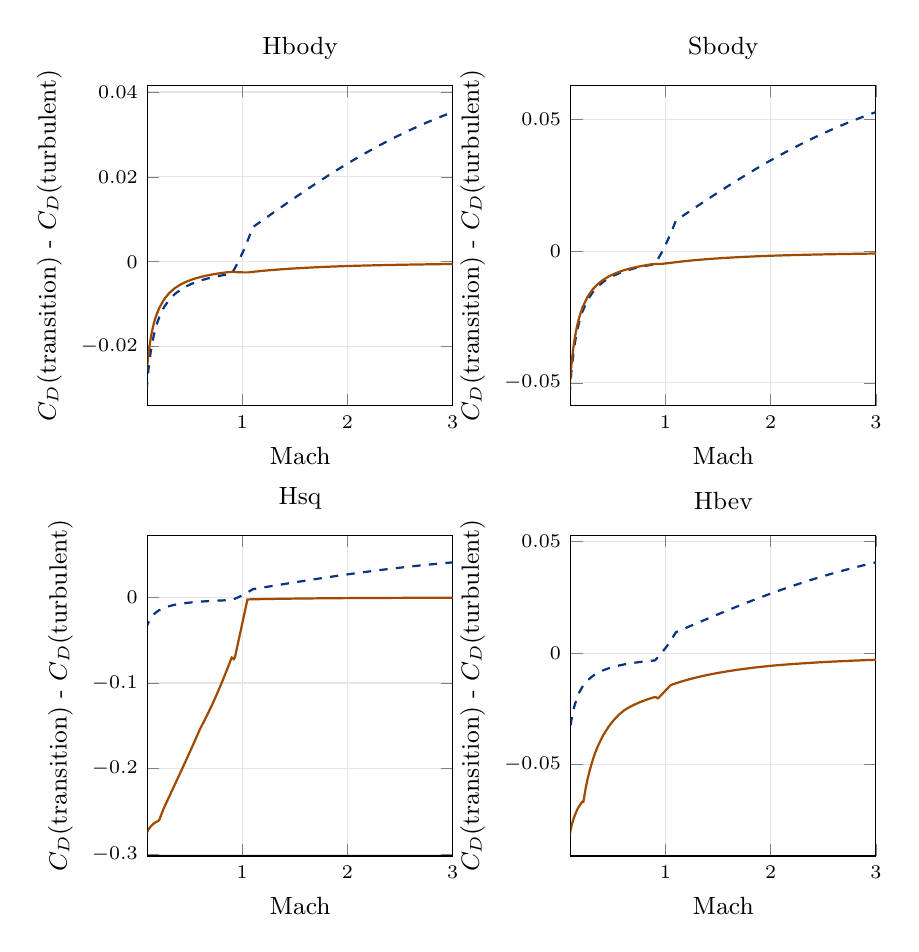
\begin{tikzpicture}
\begin{groupplot}[group style={group size=2 by 2,horizontal sep=1.50cm,vertical sep=1.65cm},width=.45\textwidth,height=5.65cm,grid=major,grid style={gray!20},tick label style={font=\scriptsize},label style={font=\small},title style={font=\small},scaled y ticks=false,yticklabel style={/pgf/number format/fixed,/pgf/number format/precision=3},unbounded coords=jump]
\nextgroupplot[title={Hbody},xlabel={Mach},ylabel={$C_D$(transition) - $C_D$(turbulent)},xmin=0.1,xmax=3]
\addplot[thick,B,dashed] coordinates {(0.01,-0.1827752) (0.02,-0.1383087) (0.03,-0.09219108) (0.04,-0.06912764) (0.05,-0.05528768) (0.06,-0.04606242) (0.07,-0.03947765) (0.08,-0.0345471) (0.09,-0.03071275) (0.1,-0.02763622) (0.11,-0.02511856) (0.13,-0.02124395) (0.16,-0.01724567) (0.18,-0.01531903) (0.21,-0.01311518) (0.26,-0.01056803) (0.31,-0.008838076) (0.36,-0.007584823) (0.41,-0.006633867) (0.46,-0.005886634) (0.51,-0.005283205) (0.56,-0.004785062) (0.61,-0.004366313) (0.66,-0.004008916) (0.71,-0.003699908) (0.76,-0.003429739) (0.81,-0.003191217) (0.86,-0.002978821) (0.9,-0.00282479) (0.91,-0.002408574) (0.96,-0.0001259511) (1.01,0.002502939) (1.06,0.00549021) (1.1,0.008144685) (1.11,0.008320331) (1.16,0.009198069) (1.21,0.01007454) (1.26,0.01094902) (1.31,0.01182074) (1.36,0.01268884) (1.41,0.01355246) (1.46,0.01441074) (1.51,0.0152628) (1.56,0.01610782) (1.61,0.01694498) (1.66,0.01777353) (1.71,0.01859272) (1.76,0.0194019) (1.81,0.02020043) (1.86,0.02098774) (1.91,0.0217633) (1.96,0.02252664) (2.01,0.02327734) (2.06,0.02401503) (2.11,0.02473938) (2.16,0.02545012) (2.21,0.02614701) (2.26,0.02682986) (2.31,0.02749852) (2.36,0.02815286) (2.41,0.02879283) (2.46,0.02941835) (2.51,0.03002943) (2.56,0.03062607) (2.61,0.03120832) (2.66,0.03177622) (2.71,0.03232987) (2.76,0.03286938) (2.81,0.03339486) (2.86,0.03390646) (2.91,0.03440433) (2.96,0.03488863) (3,0.03526643)};
\addplot[thick,burntorange] coordinates {(0.01,-0.1629181) (0.02,-0.1190684) (0.03,-0.08030526) (0.04,-0.06024751) (0.05,-0.04808461) (0.06,-0.0399434) (0.07,-0.0341203) (0.08,-0.02975263) (0.09,-0.0263576) (0.1,-0.02364425) (0.11,-0.02142695) (0.13,-0.01802255) (0.14,-0.0166881) (0.16,-0.01452436) (0.18,-0.01284645) (0.21,-0.01093566) (0.26,-0.008742706) (0.31,-0.007266677) (0.36,-0.006206912) (0.41,-0.005409946) (0.46,-0.004789351) (0.51,-0.004292769) (0.56,-0.003886641) (0.61,-0.003548488) (0.66,-0.003262689) (0.71,-0.003018048) (0.76,-0.002806344) (0.81,-0.002621401) (0.86,-0.002458488) (0.91,-0.002357441) (0.96,-0.002465106) (1.01,-0.002499496) (1.06,-0.002496677) (1.11,-0.00235322) (1.16,-0.00222213) (1.21,-0.002101874) (1.26,-0.001991162) (1.31,-0.001888901) (1.36,-0.00179416) (1.41,-0.001706138) (1.46,-0.001624144) (1.51,-0.001547581) (1.56,-0.001475926) (1.61,-0.001408721) (1.66,-0.001345565) (1.71,-0.001286102) (1.76,-0.001230017) (1.81,-0.001177032) (1.86,-0.001126894) (1.91,-0.001079382) (1.96,-0.001034294) (2.01,-0.0009925462) (2.06,-0.0009569685) (2.11,-0.0009231453) (2.16,-0.0008909622) (2.21,-0.0008603148) (2.26,-0.0008311075) (2.31,-0.0008032517) (2.36,-0.0007766665) (2.41,-0.000751277) (2.46,-0.0007270138) (2.51,-0.000703813) (2.56,-0.0006816149) (2.61,-0.0006603642) (2.66,-0.0006400093) (2.71,-0.0006205026) (2.76,-0.0006017991) (2.81,-0.0005838569) (2.86,-0.000566637) (2.91,-0.0005501026) (2.96,-0.0005342196) (3,-0.0005219606)};
\nextgroupplot[title={Sbody},xlabel={Mach},ylabel={$C_D$(transition) - $C_D$(turbulent)},xmin=0.1,xmax=3]
\addplot[thick,B,dashed] coordinates {(0.01,-0.2688682) (0.02,-0.243195) (0.03,-0.1621071) (0.04,-0.1215521) (0.05,-0.09721361) (0.06,-0.08098584) (0.07,-0.06939662) (0.08,-0.06071091) (0.09,-0.05396569) (0.1,-0.04858393) (0.11,-0.04416674) (0.13,-0.03735389) (0.14,-0.03467638) (0.16,-0.03032359) (0.18,-0.02693593) (0.21,-0.02306084) (0.26,-0.01858209) (0.31,-0.01554026) (0.36,-0.01333663) (0.41,-0.01166453) (0.46,-0.01035065) (0.51,-0.009289624) (0.56,-0.008413722) (0.61,-0.007677424) (0.66,-0.007049001) (0.71,-0.006505663) (0.76,-0.006030617) (0.81,-0.005611216) (0.86,-0.005237754) (0.9,-0.004966916) (0.91,-0.004333882) (0.96,-0.0008693112) (1.01,0.003110274) (1.06,0.007623562) (1.1,0.01162867) (1.11,0.01189853) (1.16,0.01324556) (1.21,0.01458829) (1.26,0.01592594) (1.31,0.01725754) (1.36,0.01858204) (1.41,0.0198983) (1.46,0.02120516) (1.51,0.02250145) (1.56,0.02378602) (1.61,0.02505778) (1.66,0.02631564) (1.71,0.0275586) (1.76,0.02878571) (1.81,0.0299961) (1.86,0.03118895) (1.91,0.03236353) (1.96,0.03351918) (2.01,0.0346553) (2.06,0.03577137) (2.11,0.03686694) (2.16,0.03794162) (2.21,0.0389951) (2.26,0.0400271) (2.31,0.04103742) (2.36,0.04202592) (2.41,0.04299249) (2.46,0.04393709) (2.51,0.04485971) (2.56,0.04576038) (2.61,0.04663917) (2.66,0.0474962) (2.71,0.04833161) (2.76,0.04914556) (2.81,0.04993825) (2.86,0.0507099) (2.91,0.05146076) (2.96,0.05219108) (3,0.05276074)};
\addplot[thick,burntorange] coordinates {(0.01,-0.2618697) (0.02,-0.2279626) (0.03,-0.1537241) (0.04,-0.1155109) (0.05,-0.09237922) (0.06,-0.07690084) (0.07,-0.06582631) (0.08,-0.0575146) (0.09,-0.05104887) (0.1,-0.04587699) (0.11,-0.04164684) (0.12,-0.03812332) (0.13,-0.03514343) (0.14,-0.03259071) (0.16,-0.02844627) (0.18,-0.02522692) (0.21,-0.02155344) (0.26,-0.0173251) (0.31,-0.01446923) (0.36,-0.0124123) (0.41,-0.01086101) (0.46,-0.009649822) (0.51,-0.008678263) (0.56,-0.007881852) (0.61,-0.007217298) (0.66,-0.006654471) (0.71,-0.006171764) (0.76,-0.00575327) (0.81,-0.005387023) (0.86,-0.005063858) (0.91,-0.004864341) (0.96,-0.004877245) (1.01,-0.004649272) (1.06,-0.00441328) (1.11,-0.004159696) (1.16,-0.003927974) (1.21,-0.003715402) (1.26,-0.0035197) (1.31,-0.003338938) (1.36,-0.003171468) (1.41,-0.003015874) (1.46,-0.002870937) (1.51,-0.0027356) (1.56,-0.002608937) (1.61,-0.002490142) (1.66,-0.002378503) (1.71,-0.002273392) (1.76,-0.002174254) (1.81,-0.002080594) (1.86,-0.001991968) (1.91,-0.001907983) (1.96,-0.001828282) (2.01,-0.001754486) (2.06,-0.001691597) (2.11,-0.001631809) (2.16,-0.00157492) (2.21,-0.001520746) (2.26,-0.001469117) (2.31,-0.001419877) (2.36,-0.001372884) (2.41,-0.001328003) (2.46,-0.001285114) (2.51,-0.001244103) (2.56,-0.001204864) (2.61,-0.0011673) (2.66,-0.00113132) (2.71,-0.001096839) (2.76,-0.001063777) (2.81,-0.001032061) (2.86,-0.001001622) (2.91,-0.0009723954) (2.96,-0.0009443198) (3,-0.0009226496)};
\nextgroupplot[title={Hsq},xlabel={Mach},ylabel={$C_D$(transition) - $C_D$(turbulent)},xmin=0.1,xmax=3]
\addplot[thick,B,dashed] coordinates {(0.01,-0.2108059) (0.02,-0.1595199) (0.03,-0.1063296) (0.04,-0.07972913) (0.05,-0.06376665) (0.06,-0.0531266) (0.07,-0.04553199) (0.08,-0.03984528) (0.09,-0.03542289) (0.1,-0.03187454) (0.11,-0.02897076) (0.13,-0.02450194) (0.16,-0.01989048) (0.18,-0.01766837) (0.21,-0.01512654) (0.26,-0.01218875) (0.31,-0.01019349) (0.36,-0.008748039) (0.41,-0.007651244) (0.46,-0.006789415) (0.51,-0.006093443) (0.56,-0.005518904) (0.61,-0.005035936) (0.66,-0.004623728) (0.71,-0.00426733) (0.76,-0.003955728) (0.81,-0.003680625) (0.86,-0.003435657) (0.9,-0.003258003) (0.91,-0.002777955) (0.96,-0.000145267) (1.01,0.002886792) (1.06,0.006332195) (1.1,0.009393762) (1.11,0.009596346) (1.16,0.01060869) (1.21,0.01161958) (1.26,0.01262817) (1.31,0.01363358) (1.36,0.01463481) (1.41,0.01563088) (1.46,0.01662078) (1.51,0.01760352) (1.56,0.01857813) (1.61,0.01954368) (1.66,0.02049929) (1.71,0.02144412) (1.76,0.0223774) (1.81,0.02329839) (1.86,0.02420644) (1.91,0.02510094) (1.96,0.02598135) (2.01,0.02684718) (2.06,0.027698) (2.11,0.02853344) (2.16,0.02935318) (2.21,0.03015694) (2.26,0.03094452) (2.31,0.03171572) (2.36,0.03247042) (2.41,0.03320852) (2.46,0.03392998) (2.51,0.03463478) (2.56,0.03532292) (2.61,0.03599446) (2.66,0.03664946) (2.71,0.03728802) (2.76,0.03791026) (2.81,0.03851633) (2.86,0.03910639) (2.91,0.03968061) (2.96,0.04023919) (3,0.04067492)};
\addplot[thick,burntorange] coordinates {(0.01,-0.4121075) (0.02,-0.3682577) (0.03,-0.3294946) (0.04,-0.3094368) (0.05,-0.297274) (0.06,-0.2891327) (0.07,-0.2833096) (0.08,-0.278942) (0.09,-0.2755469) (0.11,-0.2706163) (0.13,-0.2672119) (0.16,-0.2637137) (0.21,-0.260125) (0.25,-0.2473101) (0.26,-0.2446281) (0.31,-0.2313895) (0.36,-0.2182537) (0.41,-0.205067) (0.46,-0.1917427) (0.51,-0.178229) (0.56,-0.164492) (0.6,-0.1533262) (0.61,-0.151054) (0.66,-0.1391067) (0.71,-0.1263394) (0.76,-0.1127441) (0.81,-0.09831449) (0.86,-0.0830461) (0.9,-0.07022467) (0.91,-0.0707022) (0.92,-0.07213478) (0.93,-0.07038193) (0.96,-0.0534182) (1.01,-0.02514531) (1.05,-0.002527008) (1.06,-0.002496677) (1.11,-0.00235322) (1.16,-0.00222213) (1.21,-0.002101874) (1.26,-0.001991162) (1.31,-0.001888901) (1.36,-0.00179416) (1.41,-0.001706138) (1.46,-0.001624144) (1.51,-0.001547581) (1.56,-0.001475926) (1.61,-0.001408721) (1.66,-0.001345565) (1.71,-0.001286102) (1.76,-0.001230017) (1.81,-0.001177032) (1.86,-0.001126894) (1.91,-0.001079382) (1.96,-0.001034294) (2.01,-0.0009925462) (2.06,-0.0009569685) (2.11,-0.0009231453) (2.16,-0.0008909622) (2.21,-0.0008603148) (2.26,-0.0008311075) (2.31,-0.0008032517) (2.36,-0.0007766665) (2.41,-0.000751277) (2.46,-0.0007270138) (2.51,-0.000703813) (2.56,-0.0006816149) (2.61,-0.0006603642) (2.66,-0.0006400093) (2.71,-0.0006205026) (2.76,-0.0006017991) (2.81,-0.0005838569) (2.86,-0.000566637) (2.91,-0.0005501026) (2.96,-0.0005342196) (3,-0.0005219606)};
\nextgroupplot[title={Hbev},xlabel={Mach},ylabel={$C_D$(transition) - $C_D$(turbulent)},xmin=0.1,xmax=3]
\addplot[thick,B,dashed] coordinates {(0.01,-0.2108059) (0.02,-0.1595199) (0.03,-0.1063296) (0.04,-0.07972913) (0.05,-0.06376665) (0.06,-0.0531266) (0.07,-0.04553199) (0.08,-0.03984528) (0.09,-0.03542289) (0.1,-0.03187454) (0.11,-0.02897076) (0.13,-0.02450194) (0.16,-0.01989048) (0.18,-0.01766837) (0.21,-0.01512654) (0.26,-0.01218875) (0.31,-0.01019349) (0.36,-0.008748039) (0.41,-0.007651244) (0.46,-0.006789415) (0.51,-0.006093443) (0.56,-0.005518904) (0.61,-0.005035936) (0.66,-0.004623728) (0.71,-0.00426733) (0.76,-0.003955728) (0.81,-0.003680625) (0.86,-0.003435657) (0.9,-0.003258003) (0.91,-0.002777955) (0.96,-0.000145267) (1.01,0.002886792) (1.06,0.006332195) (1.1,0.009393762) (1.11,0.009596346) (1.16,0.01060869) (1.21,0.01161958) (1.26,0.01262817) (1.31,0.01363358) (1.36,0.01463481) (1.41,0.01563088) (1.46,0.01662078) (1.51,0.01760352) (1.56,0.01857813) (1.61,0.01954368) (1.66,0.02049929) (1.71,0.02144412) (1.76,0.0223774) (1.81,0.02329839) (1.86,0.02420644) (1.91,0.02510094) (1.96,0.02598135) (2.01,0.02684718) (2.06,0.027698) (2.11,0.02853344) (2.16,0.02935318) (2.21,0.03015694) (2.26,0.03094452) (2.31,0.03171572) (2.36,0.03247042) (2.41,0.03320852) (2.46,0.03392998) (2.51,0.03463478) (2.56,0.03532292) (2.61,0.03599446) (2.66,0.03664946) (2.71,0.03728802) (2.76,0.03791026) (2.81,0.03851633) (2.86,0.03910639) (2.91,0.03968061) (2.96,0.04023919) (3,0.04067492)};
\addplot[thick,burntorange] coordinates {(0.01,-0.1882793) (0.02,-0.16052) (0.03,-0.127714) (0.04,-0.1106965) (0.05,-0.1003248) (0.06,-0.09332677) (0.07,-0.08826947) (0.08,-0.08443018) (0.09,-0.08140565) (0.1,-0.07895325) (0.11,-0.07691853) (0.13,-0.07372078) (0.16,-0.07029794) (0.18,-0.0685827) (0.21,-0.06654462) (0.22,-0.06665713) (0.24,-0.06106288) (0.26,-0.05643662) (0.28,-0.05257066) (0.31,-0.04770956) (0.33,-0.04496123) (0.36,-0.04141301) (0.41,-0.03665647) (0.46,-0.03293707) (0.51,-0.02994934) (0.56,-0.02749687) (0.61,-0.02552906) (0.66,-0.02414732) (0.71,-0.02296106) (0.76,-0.02193164) (0.81,-0.02102997) (0.86,-0.02023364) (0.9,-0.0196606) (0.91,-0.01979429) (0.93,-0.02024964) (0.96,-0.01877039) (1.01,-0.01630497) (1.05,-0.01433264) (1.06,-0.01416061) (1.11,-0.01334695) (1.16,-0.01260343) (1.21,-0.01192137) (1.26,-0.01129344) (1.31,-0.01071343) (1.36,-0.01017608) (1.41,-0.00967684) (1.46,-0.009211791) (1.51,-0.00877754) (1.56,-0.008371128) (1.61,-0.007989957) (1.66,-0.007631748) (1.71,-0.007294488) (1.76,-0.00697639) (1.81,-0.006675866) (1.86,-0.006391499) (1.91,-0.006122021) (1.96,-0.005866292) (2.01,-0.005629505) (2.06,-0.005427716) (2.11,-0.005235878) (2.16,-0.005053343) (2.21,-0.004879518) (2.26,-0.00471386) (2.31,-0.004555868) (2.36,-0.004405083) (2.41,-0.004261079) (2.46,-0.004123464) (2.51,-0.003991874) (2.56,-0.003865971) (2.61,-0.003745441) (2.66,-0.003629993) (2.71,-0.003519355) (2.76,-0.003413273) (2.81,-0.003311508) (2.86,-0.003213841) (2.91,-0.003120062) (2.96,-0.003029977) (3,-0.002960447)};
\end{groupplot}\end{tikzpicture}
\caption{Subtracting the fully turbulent baseline separates the change due to each program's flow option from the baseline pressure-drag disagreement.}\label{fig:atlas-20-transition-increment}
\end{figure}
\noindent{\footnotesize Export files: \code{20-transition-increment.svg} and \code{20-transition-increment.png}.\\ Directory: \code{aerodynamic-investigation/extended/figures/}.}

\clearpage\subsubsection*{Isolated fin response to flow transition}
\begin{figure}[H]\centering
{\footnotesize\begin{tabular}{ll}
\tikz[baseline=-.5ex]{\draw[thick,B,dashed] (0,0)--(.40,0);}\ MIT OR & \tikz[baseline=-.5ex]{\draw[thick,burntorange] (0,0)--(.40,0);}\ RASAero\\
\end{tabular}}\par\vspace{.7em}
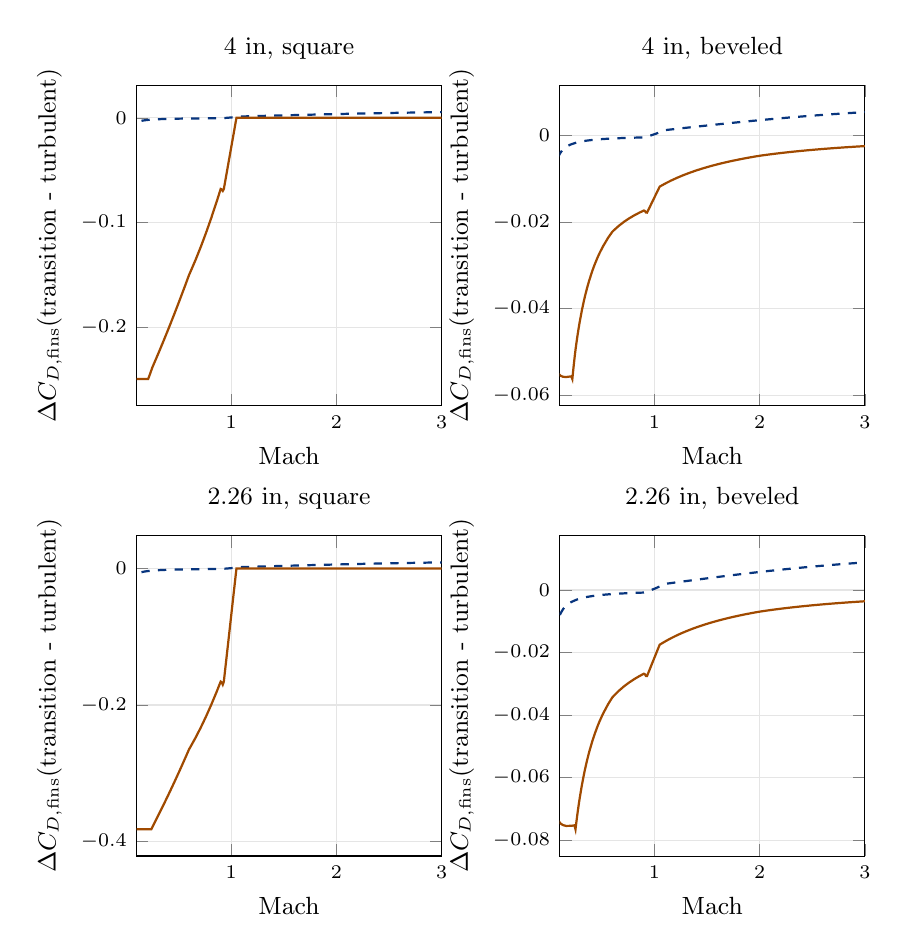
\begin{tikzpicture}
\begin{groupplot}[group style={group size=2 by 2,horizontal sep=1.50cm,vertical sep=1.65cm},width=.45\textwidth,height=5.65cm,grid=major,grid style={gray!20},tick label style={font=\scriptsize},label style={font=\small},title style={font=\small},scaled y ticks=false,yticklabel style={/pgf/number format/fixed,/pgf/number format/precision=3},unbounded coords=jump]
\nextgroupplot[title={4 in, square},xlabel={Mach},ylabel={$\Delta C_{D,\mathrm{fins}}$(transition - turbulent)},xmin=0.1,xmax=3]
\addplot[thick,B,dashed] coordinates {(0.01,-0.0280306) (0.02,-0.02121117) (0.03,-0.01413852) (0.04,-0.01060149) (0.05,-0.008478975) (0.06,-0.00706418) (0.07,-0.006054334) (0.08,-0.005298179) (0.09,-0.00471014) (0.1,-0.00423832) (0.11,-0.003852208) (0.13,-0.003257994) (0.16,-0.002644813) (0.18,-0.002349342) (0.21,-0.002011358) (0.26,-0.001620724) (0.31,-0.001355417) (0.36,-0.001163216) (0.41,-0.001017377) (0.46,-0.0009027804) (0.51,-0.0008102379) (0.56,-0.000733842) (0.61,-0.0006696224) (0.66,-0.0006148115) (0.71,-0.0005674218) (0.76,-0.0005259884) (0.81,-0.0004894084) (0.86,-0.0004568352) (0.9,-0.0004332127) (0.91,-0.0003693814) (0.96,-1.931598e-05) (1.01,0.0003838533) (1.06,0.0008419844) (1.1,0.001249077) (1.11,0.001276015) (1.16,0.001410625) (1.21,0.001545041) (1.26,0.001679153) (1.31,0.00181284) (1.36,0.001945973) (1.41,0.00207842) (1.46,0.002210046) (1.51,0.002340719) (1.56,0.002470312) (1.61,0.0025987) (1.66,0.002725766) (1.71,0.002851399) (1.76,0.002975496) (1.81,0.003097959) (1.86,0.003218701) (1.91,0.003337642) (1.96,0.003454709) (2.01,0.003569837) (2.06,0.00368297) (2.11,0.003794058) (2.16,0.003903057) (2.21,0.004009933) (2.26,0.004114655) (2.31,0.004217201) (2.36,0.004317553) (2.41,0.004415698) (2.46,0.004511629) (2.51,0.004605345) (2.56,0.004696846) (2.61,0.00478614) (2.66,0.004873234) (2.71,0.004958143) (2.76,0.005040883) (2.81,0.005121471) (2.86,0.00519993) (2.91,0.005276283) (2.96,0.005350557) (3,0.005408496)};
\addplot[thick,burntorange] coordinates {(0.01,-0.2491893) (0.06,-0.2491893) (0.11,-0.2491893) (0.16,-0.2491893) (0.18,-0.2491893) (0.21,-0.2491893) (0.22,-0.246707) (0.25,-0.2382001) (0.26,-0.2358854) (0.31,-0.2241228) (0.36,-0.2120468) (0.41,-0.199657) (0.46,-0.1869534) (0.51,-0.1739362) (0.56,-0.1606053) (0.6,-0.1497146) (0.61,-0.1475055) (0.66,-0.135844) (0.71,-0.1233214) (0.76,-0.1099377) (0.81,-0.09569309) (0.86,-0.08058762) (0.9,-0.06788315) (0.91,-0.06834475) (0.92,-0.06972957) (0.93,-0.06793746) (0.96,-0.05095309) (1.01,-0.02264582) (1.05,0) (1.06,0) (1.08,1.110223e-16) (1.11,-5.551115e-17) (1.16,0) (1.21,5.551115e-17) (1.26,0) (1.31,-5.551115e-17) (1.36,5.551115e-17) (1.41,1.110223e-16) (1.46,-5.551115e-17) (1.51,-5.551115e-17) (1.56,0) (1.61,0) (1.66,-5.551115e-17) (1.71,0) (1.76,5.551115e-17) (1.81,5.551115e-17) (1.86,5.551115e-17) (1.91,-5.551115e-17) (1.96,0) (2.01,-1.110223e-16) (2.06,0) (2.11,-5.551115e-17) (2.16,0) (2.21,-5.551115e-17) (2.26,5.551115e-17) (2.31,0) (2.36,-5.551115e-17) (2.41,-5.551115e-17) (2.46,-5.551115e-17) (2.51,0) (2.56,5.551115e-17) (2.61,0) (2.66,-5.551115e-17) (2.71,-5.551115e-17) (2.76,5.551115e-17) (2.81,0) (2.86,5.551115e-17) (2.91,5.551115e-17) (2.96,0) (3,0)};
\nextgroupplot[title={4 in, beveled},xlabel={Mach},ylabel={$\Delta C_{D,\mathrm{fins}}$(transition - turbulent)},xmin=0.1,xmax=3]
\addplot[thick,B,dashed] coordinates {(0.01,-0.0280306) (0.02,-0.02121117) (0.03,-0.01413852) (0.04,-0.01060149) (0.05,-0.008478975) (0.06,-0.00706418) (0.07,-0.006054334) (0.08,-0.005298179) (0.09,-0.00471014) (0.1,-0.00423832) (0.11,-0.003852208) (0.13,-0.003257994) (0.16,-0.002644813) (0.18,-0.002349342) (0.21,-0.002011358) (0.26,-0.001620724) (0.31,-0.001355417) (0.36,-0.001163216) (0.41,-0.001017377) (0.46,-0.0009027804) (0.51,-0.0008102379) (0.56,-0.000733842) (0.61,-0.0006696224) (0.66,-0.0006148115) (0.71,-0.0005674218) (0.76,-0.0005259884) (0.81,-0.0004894084) (0.86,-0.0004568352) (0.9,-0.0004332127) (0.91,-0.0003693814) (0.96,-1.931598e-05) (1.01,0.0003838533) (1.06,0.0008419844) (1.1,0.001249077) (1.11,0.001276015) (1.16,0.001410625) (1.21,0.001545041) (1.26,0.001679153) (1.31,0.00181284) (1.36,0.001945973) (1.41,0.00207842) (1.46,0.002210046) (1.51,0.002340719) (1.56,0.002470312) (1.61,0.0025987) (1.66,0.002725766) (1.71,0.002851399) (1.76,0.002975496) (1.81,0.003097959) (1.86,0.003218701) (1.91,0.003337642) (1.96,0.003454709) (2.01,0.003569837) (2.06,0.00368297) (2.11,0.003794058) (2.16,0.003903057) (2.21,0.004009933) (2.26,0.004114655) (2.31,0.004217201) (2.36,0.004317553) (2.41,0.004415698) (2.46,0.004511629) (2.51,0.004605345) (2.56,0.004696846) (2.61,0.00478614) (2.66,0.004873234) (2.71,0.004958143) (2.76,0.005040883) (2.81,0.005121471) (2.86,0.00519993) (2.91,0.005276283) (2.96,0.005350557) (3,0.005408496)};
\addplot[thick,burntorange] coordinates {(0.01,-0.02536115) (0.02,-0.04145157) (0.03,-0.04740869) (0.04,-0.05044902) (0.05,-0.05224023) (0.06,-0.05338337) (0.07,-0.05414917) (0.08,-0.05467755) (0.09,-0.05504805) (0.11,-0.05549157) (0.13,-0.05569823) (0.16,-0.05577358) (0.21,-0.05560896) (0.22,-0.05624108) (0.23,-0.0537958) (0.24,-0.05155433) (0.25,-0.04949216) (0.26,-0.04769391) (0.27,-0.04602883) (0.28,-0.04448273) (0.29,-0.04304328) (0.31,-0.04044288) (0.33,-0.03815772) (0.34,-0.03711598) (0.36,-0.03520609) (0.38,-0.03349723) (0.41,-0.03124652) (0.43,-0.02992053) (0.46,-0.02814772) (0.48,-0.02708897) (0.51,-0.02565658) (0.56,-0.02361023) (0.6,-0.02221873) (0.61,-0.02198057) (0.66,-0.02088463) (0.71,-0.01994301) (0.76,-0.01912529) (0.81,-0.01840857) (0.86,-0.01777516) (0.9,-0.01731908) (0.91,-0.01743685) (0.92,-0.01779016) (0.93,-0.01780516) (0.96,-0.01630528) (1.01,-0.01380547) (1.05,-0.01180563) (1.06,-0.01166393) (1.11,-0.01099373) (1.16,-0.01038131) (1.21,-0.009819494) (1.26,-0.009302274) (1.31,-0.008824534) (1.36,-0.008381922) (1.41,-0.007970702) (1.46,-0.007587647) (1.51,-0.00722996) (1.56,-0.006895202) (1.61,-0.006581236) (1.66,-0.006286183) (1.71,-0.006008386) (1.76,-0.005746372) (1.81,-0.005498834) (1.86,-0.005264604) (1.91,-0.005042639) (1.96,-0.004831997) (2.01,-0.004636959) (2.06,-0.004470748) (2.11,-0.004312733) (2.16,-0.004162381) (2.21,-0.004019203) (2.26,-0.003882753) (2.31,-0.003752617) (2.36,-0.003628416) (2.41,-0.003509802) (2.46,-0.00339645) (2.51,-0.003288061) (2.56,-0.003184356) (2.61,-0.003085077) (2.66,-0.002989984) (2.71,-0.002898852) (2.76,-0.002811474) (2.81,-0.002727652) (2.86,-0.002647204) (2.91,-0.002569959) (2.96,-0.002495757) (3,-0.002438486)};
\nextgroupplot[title={2.26 in, square},xlabel={Mach},ylabel={$\Delta C_{D,\mathrm{fins}}$(transition - turbulent)},xmin=0.1,xmax=3]
\addplot[thick,B,dashed] coordinates {(0.01,-0.04490605) (0.02,-0.04061814) (0.03,-0.02707494) (0.04,-0.02030149) (0.05,-0.0162365) (0.06,-0.01352616) (0.07,-0.01159054) (0.08,-0.01013986) (0.09,-0.009013285) (0.1,-0.00811443) (0.11,-0.007376676) (0.13,-0.006238803) (0.14,-0.005791607) (0.16,-0.00506461) (0.18,-0.004498806) (0.21,-0.003851593) (0.26,-0.003103559) (0.31,-0.002595516) (0.36,-0.002227468) (0.41,-0.001948197) (0.46,-0.001728753) (0.51,-0.001551542) (0.56,-0.00140525) (0.61,-0.001282274) (0.66,-0.001177316) (0.71,-0.001086568) (0.76,-0.001007226) (0.81,-0.0009371786) (0.86,-0.0008748034) (0.9,-0.0008295684) (0.91,-0.0007238399) (0.96,-0.0001451913) (1.01,0.0005194743) (1.06,0.001273278) (1.1,0.001942206) (1.11,0.001987279) (1.16,0.002212257) (1.21,0.002436519) (1.26,0.002659931) (1.31,0.002882335) (1.36,0.003103551) (1.41,0.003323391) (1.46,0.00354166) (1.51,0.003758165) (1.56,0.003972714) (1.61,0.00418512) (1.66,0.004395206) (1.71,0.004602804) (1.76,0.004807755) (1.81,0.005009913) (1.86,0.005209141) (1.91,0.005405319) (1.96,0.005598333) (2.01,0.005788087) (2.06,0.005974492) (2.11,0.006157473) (2.16,0.006336965) (2.21,0.006512915) (2.26,0.006685278) (2.31,0.006854021) (2.36,0.007019119) (2.41,0.007180555) (2.46,0.007338321) (2.51,0.007492415) (2.56,0.007642843) (2.61,0.007789619) (2.66,0.007932759) (2.71,0.008072288) (2.76,0.008208233) (2.81,0.008340627) (2.86,0.008469508) (2.91,0.008594915) (2.96,0.008716892) (3,0.008812036)};
\addplot[thick,burntorange] coordinates {(0.01,-0.3821734) (0.03,-0.3821734) (0.06,-0.3821734) (0.11,-0.3821734) (0.16,-0.3821734) (0.21,-0.3821734) (0.24,-0.3821734) (0.26,-0.3759346) (0.31,-0.3608056) (0.36,-0.3452555) (0.41,-0.3292845) (0.46,-0.3128924) (0.51,-0.2960793) (0.56,-0.2788452) (0.6,-0.2647549) (0.61,-0.2621589) (0.66,-0.2483087) (0.71,-0.2333031) (0.76,-0.2171422) (0.81,-0.1998256) (0.86,-0.1813538) (0.9,-0.1657444) (0.91,-0.1668715) (0.92,-0.1702527) (0.93,-0.165877) (0.96,-0.1244078) (1.01,-0.05529234) (1.05,0) (1.06,0) (1.11,5.551115e-17) (1.16,-5.551115e-17) (1.21,5.551115e-17) (1.26,0) (1.31,-5.551115e-17) (1.36,0) (1.41,-5.551115e-17) (1.42,1.110223e-16) (1.46,0) (1.51,-5.551115e-17) (1.56,0) (1.61,0) (1.66,5.551115e-17) (1.71,5.551115e-17) (1.76,-1.110223e-16) (1.81,0) (1.86,-5.551115e-17) (1.91,5.551115e-17) (1.96,0) (2.01,-5.551115e-17) (2.06,-5.551115e-17) (2.11,5.551115e-17) (2.16,1.110223e-16) (2.21,5.551115e-17) (2.26,5.551115e-17) (2.31,0) (2.36,1.110223e-16) (2.41,5.551115e-17) (2.46,0) (2.51,-5.551115e-17) (2.56,-5.551115e-17) (2.61,-5.551115e-17) (2.66,0) (2.71,0) (2.76,5.551115e-17) (2.81,-1.110223e-16) (2.86,0) (2.91,5.551115e-17) (2.96,2.775558e-17) (3,0)};
\nextgroupplot[title={2.26 in, beveled},xlabel={Mach},ylabel={$\Delta C_{D,\mathrm{fins}}$(transition - turbulent)},xmin=0.1,xmax=3]
\addplot[thick,B,dashed] coordinates {(0.01,-0.04490605) (0.02,-0.04061814) (0.03,-0.02707494) (0.04,-0.02030149) (0.05,-0.0162365) (0.06,-0.01352616) (0.07,-0.01159054) (0.08,-0.01013986) (0.09,-0.009013285) (0.1,-0.00811443) (0.11,-0.007376676) (0.13,-0.006238803) (0.14,-0.005791607) (0.16,-0.00506461) (0.18,-0.004498806) (0.21,-0.003851593) (0.26,-0.003103559) (0.31,-0.002595516) (0.36,-0.002227468) (0.41,-0.001948197) (0.46,-0.001728753) (0.51,-0.001551542) (0.56,-0.00140525) (0.61,-0.001282274) (0.66,-0.001177316) (0.71,-0.001086568) (0.76,-0.001007226) (0.81,-0.0009371786) (0.86,-0.0008748034) (0.9,-0.0008295684) (0.91,-0.0007238399) (0.96,-0.0001451913) (1.01,0.0005194743) (1.06,0.001273278) (1.1,0.001942206) (1.11,0.001987279) (1.16,0.002212257) (1.21,0.002436519) (1.26,0.002659931) (1.31,0.002882335) (1.36,0.003103551) (1.41,0.003323391) (1.46,0.00354166) (1.51,0.003758165) (1.56,0.003972714) (1.61,0.00418512) (1.66,0.004395206) (1.71,0.004602804) (1.76,0.004807755) (1.81,0.005009913) (1.86,0.005209141) (1.91,0.005405319) (1.96,0.005598333) (2.01,0.005788087) (2.06,0.005974492) (2.11,0.006157473) (2.16,0.006336965) (2.21,0.006512915) (2.26,0.006685278) (2.31,0.006854021) (2.36,0.007019119) (2.41,0.007180555) (2.46,0.007338321) (2.51,0.007492415) (2.56,0.007642843) (2.61,0.007789619) (2.66,0.007932759) (2.71,0.008072288) (2.76,0.008208233) (2.81,0.008340627) (2.86,0.008469508) (2.91,0.008594915) (2.96,0.008716892) (3,0.008812036)};
\addplot[thick,burntorange] coordinates {(0.01,-0.02867319) (0.02,-0.05275309) (0.03,-0.06180625) (0.04,-0.0664972) (0.05,-0.06930607) (0.06,-0.07113171) (0.07,-0.07238076) (0.08,-0.07326449) (0.09,-0.0739034) (0.11,-0.07471567) (0.13,-0.07515211) (0.16,-0.07542636) (0.21,-0.07539556) (0.24,-0.07523962) (0.25,-0.07652969) (0.26,-0.07374906) (0.27,-0.0711744) (0.28,-0.06878364) (0.29,-0.06655778) (0.31,-0.06253684) (0.33,-0.05900329) (0.34,-0.05739242) (0.36,-0.05443911) (0.38,-0.05179672) (0.41,-0.04831646) (0.43,-0.04626607) (0.46,-0.04352485) (0.48,-0.04188768) (0.51,-0.0396727) (0.56,-0.03650849) (0.6,-0.03435682) (0.61,-0.03398857) (0.66,-0.03229386) (0.71,-0.03083788) (0.76,-0.02957347) (0.81,-0.02846513) (0.86,-0.02748571) (0.9,-0.02678051) (0.91,-0.02696262) (0.92,-0.02750894) (0.93,-0.02750219) (0.96,-0.02500323) (1.01,-0.0208383) (1.05,-0.01750635) (1.06,-0.01729623) (1.11,-0.0163024) (1.16,-0.01539425) (1.21,-0.01456115) (1.26,-0.01379417) (1.31,-0.01308574) (1.36,-0.0124294) (1.41,-0.01181961) (1.46,-0.01125158) (1.51,-0.01072118) (1.56,-0.01022477) (1.61,-0.009759195) (1.66,-0.009321668) (1.71,-0.008909726) (1.76,-0.008521191) (1.81,-0.008154122) (1.86,-0.007806786) (1.91,-0.007477637) (1.96,-0.007165281) (2.01,-0.006876061) (2.06,-0.00662959) (2.11,-0.006395274) (2.16,-0.006172319) (2.21,-0.005960004) (2.26,-0.005757663) (2.31,-0.005564686) (2.36,-0.005380512) (2.41,-0.005204621) (2.46,-0.005036534) (2.51,-0.004875805) (2.56,-0.004722023) (2.61,-0.004574804) (2.66,-0.004433793) (2.71,-0.004298656) (2.76,-0.004169083) (2.81,-0.004044785) (2.86,-0.003925491) (2.91,-0.003810946) (2.96,-0.003700914) (3,-0.003615986)};
\end{groupplot}\end{tikzpicture}
\caption{Subtract the body-only response to the flow option from the finned-rocket response. This isolates the net fin dependency without labeling it as a proprietary RASAero internal pressure or friction term.}\label{fig:atlas-28-fin-transition-response}
\end{figure}
\noindent{\footnotesize Export files: \code{28-fin-transition-response.svg} and \code{28-fin-transition-response.png}.\\ Directory: \code{aerodynamic-investigation/extended/figures/}.}

\clearpage\subsubsection*{Nozzle-area sensitivity: Hbody}
\begin{figure}[H]\centering
{\footnotesize\begin{tabular}{lll}
\tikz[baseline=-.5ex]{\draw[thick,B,dashed] (0,0)--(.40,0);}\ OR (no nozzle model) & \tikz[baseline=-.5ex]{\draw[thick,burntorange] (0,0)--(.40,0);}\ RAS power-off & \tikz[baseline=-.5ex]{\draw[thick,g] (0,0)--(.40,0);}\ RAS power-on\\
\end{tabular}}\par\vspace{.7em}
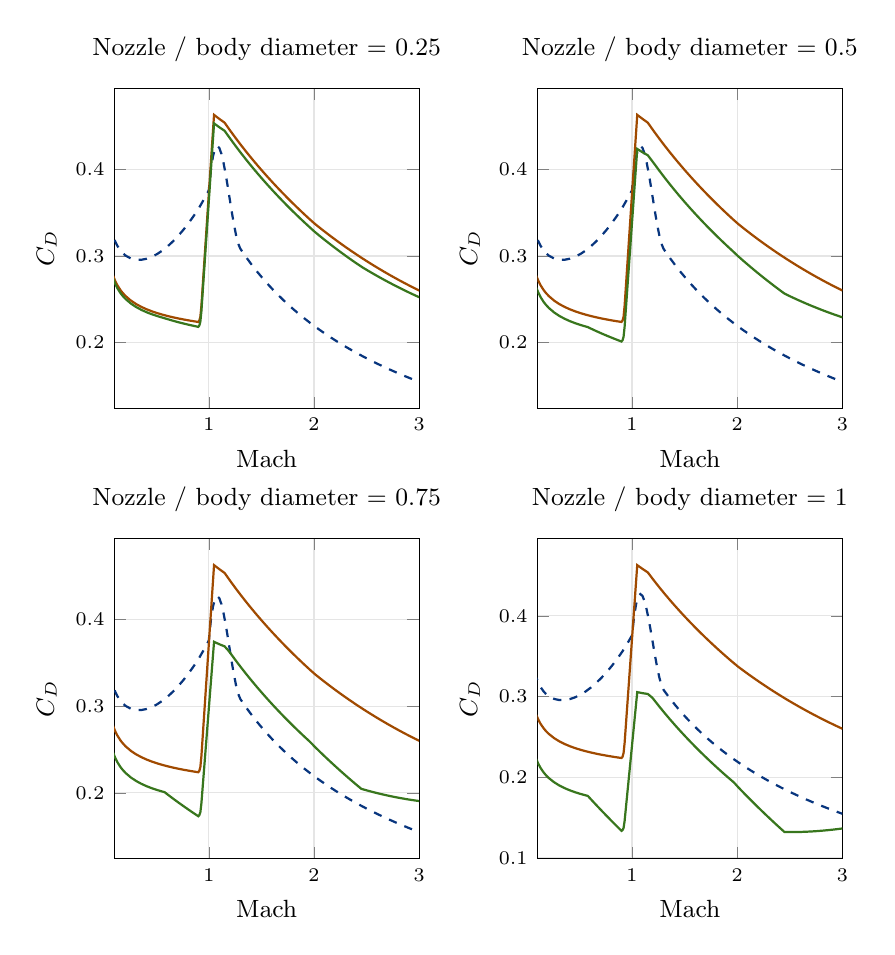
\begin{tikzpicture}
\begin{groupplot}[group style={group size=2 by 2,horizontal sep=1.50cm,vertical sep=1.65cm},width=.45\textwidth,height=5.65cm,grid=major,grid style={gray!20},tick label style={font=\scriptsize},label style={font=\small},title style={font=\small},scaled y ticks=false,yticklabel style={/pgf/number format/fixed,/pgf/number format/precision=3},unbounded coords=jump]
\nextgroupplot[title={Nozzle / body diameter = 0.25},xlabel={Mach},ylabel={$C_D$},xmin=0.1,xmax=3]
\addplot[thick,B,dashed] coordinates {(0.01,0.432385) (0.02,0.3897077) (0.03,0.368739) (0.04,0.355364) (0.05,0.3457716) (0.06,0.3384154) (0.07,0.3325257) (0.08,0.3276676) (0.09,0.3235729) (0.11,0.3170244) (0.13,0.312015) (0.16,0.3064266) (0.18,0.303622) (0.21,0.3004307) (0.26,0.2971293) (0.31,0.2956987) (0.36,0.2957129) (0.41,0.296925) (0.46,0.29918) (0.51,0.3023746) (0.56,0.3064369) (0.61,0.311315) (0.66,0.3169702) (0.71,0.3233731) (0.76,0.3305008) (0.81,0.3383351) (0.86,0.3468615) (0.91,0.3561867) (0.96,0.3667604) (1,0.3758332) (1.01,0.3876035) (1.02,0.3994312) (1.04,0.41525) (1.06,0.4241697) (1.08,0.4270714) (1.1,0.424837) (1.11,0.4213711) (1.12,0.4179431) (1.14,0.4076398) (1.16,0.3948092) (1.18,0.3803337) (1.21,0.3575234) (1.22,0.34998) (1.24,0.3358689) (1.26,0.323647) (1.28,0.3141988) (1.3,0.308409) (1.31,0.3065889) (1.36,0.2978366) (1.41,0.2896227) (1.46,0.2818902) (1.51,0.2745922) (1.56,0.2676872) (1.61,0.2611402) (1.66,0.2549197) (1.71,0.2489988) (1.76,0.2433533) (1.81,0.2379621) (1.86,0.2328059) (1.91,0.2278679) (1.96,0.2231329) (2.01,0.2185872) (2.06,0.2142184) (2.11,0.2100153) (2.16,0.2059678) (2.21,0.2020666) (2.26,0.1983031) (2.31,0.1946698) (2.36,0.1911594) (2.41,0.1877654) (2.46,0.1844817) (2.51,0.1813028) (2.56,0.1782235) (2.61,0.175239) (2.66,0.1723447) (2.71,0.1695367) (2.76,0.1668109) (2.81,0.1641637) (2.86,0.1615918) (2.91,0.1590919) (2.96,0.156661) (3,0.154764)};
\addplot[thick,burntorange] coordinates {(0.01,0.3747526) (0.02,0.3370981) (0.03,0.3184175) (0.04,0.3064439) (0.05,0.2978187) (0.06,0.2911705) (0.07,0.2858134) (0.08,0.2813592) (0.09,0.2775679) (0.11,0.2713925) (0.13,0.2665116) (0.16,0.2607559) (0.18,0.2576371) (0.21,0.2537077) (0.26,0.2485362) (0.31,0.2445031) (0.36,0.2412271) (0.41,0.238487) (0.46,0.2361445) (0.51,0.2341071) (0.56,0.2323107) (0.61,0.2307088) (0.66,0.2292669) (0.71,0.2279585) (0.76,0.2267632) (0.81,0.2256647) (0.86,0.2246499) (0.9,0.2238911) (0.91,0.2254135) (0.92,0.2299809) (0.93,0.2425879) (0.96,0.2976764) (1.01,0.3894907) (1.05,0.4629422) (1.06,0.4619899) (1.11,0.4574285) (1.15,0.4539954) (1.16,0.4522726) (1.21,0.4436996) (1.26,0.4354433) (1.31,0.4274746) (1.36,0.4197684) (1.41,0.412304) (1.46,0.4050635) (1.51,0.3980314) (1.56,0.3911943) (1.61,0.3845406) (1.66,0.3780599) (1.71,0.371743) (1.76,0.3655817) (1.81,0.3595688) (1.86,0.3536978) (1.91,0.3479626) (1.96,0.3423577) (2.01,0.336981) (2.06,0.3321207) (2.11,0.3273803) (2.16,0.3227565) (2.21,0.3182462) (2.26,0.3138469) (2.31,0.3095557) (2.36,0.3053702) (2.41,0.3012879) (2.46,0.2973064) (2.51,0.2934237) (2.56,0.2896372) (2.61,0.2859449) (2.66,0.2823448) (2.71,0.2788348) (2.76,0.2754128) (2.81,0.2720768) (2.86,0.2688251) (2.91,0.2656555) (2.96,0.2625662) (3,0.2601514)};
\addplot[thick,g] coordinates {(0.01,0.3713338) (0.02,0.3336793) (0.03,0.3149988) (0.04,0.3030251) (0.05,0.2944) (0.06,0.2877517) (0.07,0.2823947) (0.08,0.2779404) (0.09,0.2741491) (0.11,0.2679737) (0.13,0.2630928) (0.16,0.2573372) (0.18,0.2542183) (0.21,0.2502889) (0.26,0.2451174) (0.31,0.2410844) (0.36,0.2378083) (0.41,0.2350683) (0.46,0.2327257) (0.51,0.2306884) (0.56,0.228892) (0.61,0.2270814) (0.66,0.2252916) (0.71,0.2236354) (0.76,0.2220923) (0.81,0.220646) (0.86,0.2192833) (0.9,0.2182462) (0.91,0.2197303) (0.92,0.2241825) (0.93,0.2365451) (0.96,0.2906855) (1.01,0.3809195) (1.05,0.4531068) (1.06,0.4521961) (1.11,0.4478431) (1.15,0.4445766) (1.16,0.4428955) (1.21,0.4344621) (1.26,0.4262058) (1.31,0.4182371) (1.36,0.4105309) (1.41,0.4030665) (1.46,0.395826) (1.51,0.3887939) (1.56,0.3819568) (1.61,0.375303) (1.66,0.3688224) (1.71,0.3625054) (1.76,0.3563442) (1.81,0.3503313) (1.86,0.3444603) (1.91,0.3387251) (1.96,0.3331202) (2.01,0.3276487) (2.06,0.3226699) (2.11,0.317811) (2.16,0.3130687) (2.21,0.3084399) (2.26,0.3039221) (2.31,0.2995124) (2.36,0.2952085) (2.41,0.2910076) (2.46,0.2869796) (2.51,0.2833377) (2.56,0.2797921) (2.61,0.2763408) (2.66,0.2729816) (2.71,0.2697125) (2.76,0.2665314) (2.81,0.2634364) (2.86,0.2604255) (2.91,0.2574968) (2.96,0.2546484) (3,0.2524263)};
\nextgroupplot[title={Nozzle / body diameter = 0.5},xlabel={Mach},ylabel={$C_D$},xmin=0.1,xmax=3]
\addplot[thick,B,dashed] coordinates {(0.01,0.432385) (0.02,0.3897077) (0.03,0.368739) (0.04,0.355364) (0.05,0.3457716) (0.06,0.3384154) (0.07,0.3325257) (0.08,0.3276676) (0.09,0.3235729) (0.11,0.3170244) (0.13,0.312015) (0.16,0.3064266) (0.18,0.303622) (0.21,0.3004307) (0.26,0.2971293) (0.31,0.2956987) (0.36,0.2957129) (0.41,0.296925) (0.46,0.29918) (0.51,0.3023746) (0.56,0.3064369) (0.61,0.311315) (0.66,0.3169702) (0.71,0.3233731) (0.76,0.3305008) (0.81,0.3383351) (0.86,0.3468615) (0.91,0.3561867) (0.96,0.3667604) (1,0.3758332) (1.01,0.3876035) (1.02,0.3994312) (1.04,0.41525) (1.06,0.4241697) (1.08,0.4270714) (1.1,0.424837) (1.11,0.4213711) (1.12,0.4179431) (1.14,0.4076398) (1.16,0.3948092) (1.18,0.3803337) (1.21,0.3575234) (1.22,0.34998) (1.24,0.3358689) (1.26,0.323647) (1.28,0.3141988) (1.3,0.308409) (1.31,0.3065889) (1.36,0.2978366) (1.41,0.2896227) (1.46,0.2818902) (1.51,0.2745922) (1.56,0.2676872) (1.61,0.2611402) (1.66,0.2549197) (1.71,0.2489988) (1.76,0.2433533) (1.81,0.2379621) (1.86,0.2328059) (1.91,0.2278679) (1.96,0.2231329) (2.01,0.2185872) (2.06,0.2142184) (2.11,0.2100153) (2.16,0.2059678) (2.21,0.2020666) (2.26,0.1983031) (2.31,0.1946698) (2.36,0.1911594) (2.41,0.1877654) (2.46,0.1844817) (2.51,0.1813028) (2.56,0.1782235) (2.61,0.175239) (2.66,0.1723447) (2.71,0.1695367) (2.76,0.1668109) (2.81,0.1641637) (2.86,0.1615918) (2.91,0.1590919) (2.96,0.156661) (3,0.154764)};
\addplot[thick,burntorange] coordinates {(0.01,0.3747526) (0.02,0.3370981) (0.03,0.3184175) (0.04,0.3064439) (0.05,0.2978187) (0.06,0.2911705) (0.07,0.2858134) (0.08,0.2813592) (0.09,0.2775679) (0.11,0.2713925) (0.13,0.2665116) (0.16,0.2607559) (0.18,0.2576371) (0.21,0.2537077) (0.26,0.2485362) (0.31,0.2445031) (0.36,0.2412271) (0.41,0.238487) (0.46,0.2361445) (0.51,0.2341071) (0.56,0.2323107) (0.61,0.2307088) (0.66,0.2292669) (0.71,0.2279585) (0.76,0.2267632) (0.81,0.2256647) (0.86,0.2246499) (0.9,0.2238911) (0.91,0.2254135) (0.92,0.2299809) (0.93,0.2425879) (0.96,0.2976764) (1.01,0.3894907) (1.05,0.4629422) (1.06,0.4619899) (1.11,0.4574285) (1.15,0.4539954) (1.16,0.4522726) (1.21,0.4436996) (1.26,0.4354433) (1.31,0.4274746) (1.36,0.4197684) (1.41,0.412304) (1.46,0.4050635) (1.51,0.3980314) (1.56,0.3911943) (1.61,0.3845406) (1.66,0.3780599) (1.71,0.371743) (1.76,0.3655817) (1.81,0.3595688) (1.86,0.3536978) (1.91,0.3479626) (1.96,0.3423577) (2.01,0.336981) (2.06,0.3321207) (2.11,0.3273803) (2.16,0.3227565) (2.21,0.3182462) (2.26,0.3138469) (2.31,0.3095557) (2.36,0.3053702) (2.41,0.3012879) (2.46,0.2973064) (2.51,0.2934237) (2.56,0.2896372) (2.61,0.2859449) (2.66,0.2823448) (2.71,0.2788348) (2.76,0.2754128) (2.81,0.2720768) (2.86,0.2688251) (2.91,0.2656555) (2.96,0.2625662) (3,0.2601514)};
\addplot[thick,g] coordinates {(0.01,0.3610775) (0.02,0.3234231) (0.03,0.3047425) (0.04,0.2927689) (0.05,0.2841437) (0.06,0.2774955) (0.07,0.2721384) (0.08,0.2676841) (0.09,0.2638929) (0.11,0.2577174) (0.13,0.2528365) (0.16,0.2470809) (0.18,0.243962) (0.21,0.2400326) (0.26,0.2348612) (0.31,0.2308281) (0.36,0.227552) (0.41,0.224812) (0.46,0.2224695) (0.51,0.2204321) (0.56,0.2186357) (0.58,0.2179738) (0.61,0.216199) (0.66,0.2133658) (0.71,0.2106661) (0.76,0.2080795) (0.81,0.2055897) (0.86,0.2031836) (0.9,0.2013117) (0.91,0.2026806) (0.92,0.2067874) (0.93,0.2184167) (0.96,0.2697127) (1.01,0.3552059) (1.05,0.4236005) (1.06,0.4228148) (1.11,0.4190868) (1.15,0.4163203) (1.16,0.4147642) (1.21,0.4067495) (1.26,0.3984933) (1.31,0.3905245) (1.36,0.3828184) (1.41,0.375354) (1.46,0.3681135) (1.51,0.3610813) (1.56,0.3542442) (1.61,0.3475905) (1.66,0.3411098) (1.71,0.3347929) (1.76,0.3286317) (1.81,0.3226187) (1.86,0.3167478) (1.91,0.3110126) (1.96,0.3054076) (2.01,0.2996518) (2.06,0.2943176) (2.11,0.2891031) (2.16,0.2840054) (2.21,0.2790211) (2.26,0.2741478) (2.31,0.2693827) (2.36,0.2647233) (2.41,0.260167) (2.45,0.2565948) (2.46,0.2559991) (2.51,0.25308) (2.56,0.2502571) (2.61,0.2475285) (2.66,0.244892) (2.71,0.2423456) (2.76,0.2398873) (2.81,0.2375149) (2.86,0.2352268) (2.91,0.2330209) (2.96,0.2308952) (3,0.2292513)};
\nextgroupplot[title={Nozzle / body diameter = 0.75},xlabel={Mach},ylabel={$C_D$},xmin=0.1,xmax=3]
\addplot[thick,B,dashed] coordinates {(0.01,0.432385) (0.02,0.3897077) (0.03,0.368739) (0.04,0.355364) (0.05,0.3457716) (0.06,0.3384154) (0.07,0.3325257) (0.08,0.3276676) (0.09,0.3235729) (0.11,0.3170244) (0.13,0.312015) (0.16,0.3064266) (0.18,0.303622) (0.21,0.3004307) (0.26,0.2971293) (0.31,0.2956987) (0.36,0.2957129) (0.41,0.296925) (0.46,0.29918) (0.51,0.3023746) (0.56,0.3064369) (0.61,0.311315) (0.66,0.3169702) (0.71,0.3233731) (0.76,0.3305008) (0.81,0.3383351) (0.86,0.3468615) (0.91,0.3561867) (0.96,0.3667604) (1,0.3758332) (1.01,0.3876035) (1.02,0.3994312) (1.04,0.41525) (1.06,0.4241697) (1.08,0.4270714) (1.1,0.424837) (1.11,0.4213711) (1.12,0.4179431) (1.14,0.4076398) (1.16,0.3948092) (1.18,0.3803337) (1.21,0.3575234) (1.22,0.34998) (1.24,0.3358689) (1.26,0.323647) (1.28,0.3141988) (1.3,0.308409) (1.31,0.3065889) (1.36,0.2978366) (1.41,0.2896227) (1.46,0.2818902) (1.51,0.2745922) (1.56,0.2676872) (1.61,0.2611402) (1.66,0.2549197) (1.71,0.2489988) (1.76,0.2433533) (1.81,0.2379621) (1.86,0.2328059) (1.91,0.2278679) (1.96,0.2231329) (2.01,0.2185872) (2.06,0.2142184) (2.11,0.2100153) (2.16,0.2059678) (2.21,0.2020666) (2.26,0.1983031) (2.31,0.1946698) (2.36,0.1911594) (2.41,0.1877654) (2.46,0.1844817) (2.51,0.1813028) (2.56,0.1782235) (2.61,0.175239) (2.66,0.1723447) (2.71,0.1695367) (2.76,0.1668109) (2.81,0.1641637) (2.86,0.1615918) (2.91,0.1590919) (2.96,0.156661) (3,0.154764)};
\addplot[thick,burntorange] coordinates {(0.01,0.3747526) (0.02,0.3370981) (0.03,0.3184175) (0.04,0.3064439) (0.05,0.2978187) (0.06,0.2911705) (0.07,0.2858134) (0.08,0.2813592) (0.09,0.2775679) (0.11,0.2713925) (0.13,0.2665116) (0.16,0.2607559) (0.18,0.2576371) (0.21,0.2537077) (0.26,0.2485362) (0.31,0.2445031) (0.36,0.2412271) (0.41,0.238487) (0.46,0.2361445) (0.51,0.2341071) (0.56,0.2323107) (0.61,0.2307088) (0.66,0.2292669) (0.71,0.2279585) (0.76,0.2267632) (0.81,0.2256647) (0.86,0.2246499) (0.9,0.2238911) (0.91,0.2254135) (0.92,0.2299809) (0.93,0.2425879) (0.96,0.2976764) (1.01,0.3894907) (1.05,0.4629422) (1.06,0.4619899) (1.11,0.4574285) (1.15,0.4539954) (1.16,0.4522726) (1.21,0.4436996) (1.26,0.4354433) (1.31,0.4274746) (1.36,0.4197684) (1.41,0.412304) (1.46,0.4050635) (1.51,0.3980314) (1.56,0.3911943) (1.61,0.3845406) (1.66,0.3780599) (1.71,0.371743) (1.76,0.3655817) (1.81,0.3595688) (1.86,0.3536978) (1.91,0.3479626) (1.96,0.3423577) (2.01,0.336981) (2.06,0.3321207) (2.11,0.3273803) (2.16,0.3227565) (2.21,0.3182462) (2.26,0.3138469) (2.31,0.3095557) (2.36,0.3053702) (2.41,0.3012879) (2.46,0.2973064) (2.51,0.2934237) (2.56,0.2896372) (2.61,0.2859449) (2.66,0.2823448) (2.71,0.2788348) (2.76,0.2754128) (2.81,0.2720768) (2.86,0.2688251) (2.91,0.2656555) (2.96,0.2625662) (3,0.2601514)};
\addplot[thick,g] coordinates {(0.01,0.3439838) (0.02,0.3063293) (0.03,0.2876487) (0.04,0.2756751) (0.05,0.2670499) (0.06,0.2604017) (0.07,0.2550446) (0.08,0.2505904) (0.09,0.2467991) (0.11,0.2406237) (0.13,0.2357428) (0.16,0.2299871) (0.18,0.2268683) (0.21,0.2229389) (0.26,0.2177674) (0.31,0.2137343) (0.36,0.2104583) (0.41,0.2077182) (0.46,0.2053757) (0.51,0.2033383) (0.56,0.2015419) (0.58,0.20088) (0.61,0.1980618) (0.66,0.1934894) (0.71,0.1890506) (0.76,0.1847248) (0.81,0.1804959) (0.86,0.1763506) (0.9,0.1730874) (0.91,0.1742644) (0.92,0.1777954) (0.93,0.1882028) (0.96,0.234758) (1.01,0.3123498) (1.05,0.3744233) (1.06,0.373846) (1.11,0.3711596) (1.15,0.3692265) (1.16,0.3678787) (1.19,0.36382) (1.21,0.3605619) (1.26,0.3523057) (1.31,0.3443369) (1.36,0.3366308) (1.41,0.3291664) (1.46,0.3219259) (1.51,0.3148937) (1.56,0.3080566) (1.61,0.3014029) (1.66,0.2949222) (1.71,0.2886053) (1.76,0.2824441) (1.81,0.2764312) (1.86,0.2705602) (1.91,0.264825) (1.96,0.2592201) (2.01,0.2529903) (2.06,0.2470636) (2.11,0.2412567) (2.16,0.2355665) (2.21,0.2299898) (2.26,0.224524) (2.31,0.2191665) (2.36,0.2139146) (2.41,0.2087658) (2.45,0.2047197) (2.46,0.2043649) (2.51,0.2026503) (2.56,0.201032) (2.61,0.199508) (2.66,0.198076) (2.71,0.1967342) (2.76,0.1954804) (2.81,0.1943126) (2.86,0.193229) (2.91,0.1922276) (2.96,0.1913065) (3,0.1906262)};
\nextgroupplot[title={Nozzle / body diameter = 1},xlabel={Mach},ylabel={$C_D$},xmin=0.1,xmax=3]
\addplot[thick,B,dashed] coordinates {(0.01,0.432385) (0.02,0.3897077) (0.03,0.368739) (0.04,0.355364) (0.05,0.3457716) (0.06,0.3384154) (0.07,0.3325257) (0.08,0.3276676) (0.09,0.3235729) (0.11,0.3170244) (0.13,0.312015) (0.16,0.3064266) (0.18,0.303622) (0.21,0.3004307) (0.26,0.2971293) (0.31,0.2956987) (0.36,0.2957129) (0.41,0.296925) (0.46,0.29918) (0.51,0.3023746) (0.56,0.3064369) (0.61,0.311315) (0.66,0.3169702) (0.71,0.3233731) (0.76,0.3305008) (0.81,0.3383351) (0.86,0.3468615) (0.91,0.3561867) (0.96,0.3667604) (1,0.3758332) (1.01,0.3876035) (1.02,0.3994312) (1.04,0.41525) (1.06,0.4241697) (1.08,0.4270714) (1.1,0.424837) (1.11,0.4213711) (1.12,0.4179431) (1.14,0.4076398) (1.16,0.3948092) (1.18,0.3803337) (1.21,0.3575234) (1.22,0.34998) (1.24,0.3358689) (1.26,0.323647) (1.28,0.3141988) (1.3,0.308409) (1.31,0.3065889) (1.36,0.2978366) (1.41,0.2896227) (1.46,0.2818902) (1.51,0.2745922) (1.56,0.2676872) (1.61,0.2611402) (1.66,0.2549197) (1.71,0.2489988) (1.76,0.2433533) (1.81,0.2379621) (1.86,0.2328059) (1.91,0.2278679) (1.96,0.2231329) (2.01,0.2185872) (2.06,0.2142184) (2.11,0.2100153) (2.16,0.2059678) (2.21,0.2020666) (2.26,0.1983031) (2.31,0.1946698) (2.36,0.1911594) (2.41,0.1877654) (2.46,0.1844817) (2.51,0.1813028) (2.56,0.1782235) (2.61,0.175239) (2.66,0.1723447) (2.71,0.1695367) (2.76,0.1668109) (2.81,0.1641637) (2.86,0.1615918) (2.91,0.1590919) (2.96,0.156661) (3,0.154764)};
\addplot[thick,burntorange] coordinates {(0.01,0.3747526) (0.02,0.3370981) (0.03,0.3184175) (0.04,0.3064439) (0.05,0.2978187) (0.06,0.2911705) (0.07,0.2858134) (0.08,0.2813592) (0.09,0.2775679) (0.11,0.2713925) (0.13,0.2665116) (0.16,0.2607559) (0.18,0.2576371) (0.21,0.2537077) (0.26,0.2485362) (0.31,0.2445031) (0.36,0.2412271) (0.41,0.238487) (0.46,0.2361445) (0.51,0.2341071) (0.56,0.2323107) (0.61,0.2307088) (0.66,0.2292669) (0.71,0.2279585) (0.76,0.2267632) (0.81,0.2256647) (0.86,0.2246499) (0.9,0.2238911) (0.91,0.2254135) (0.92,0.2299809) (0.93,0.2425879) (0.96,0.2976764) (1.01,0.3894907) (1.05,0.4629422) (1.06,0.4619899) (1.11,0.4574285) (1.15,0.4539954) (1.16,0.4522726) (1.21,0.4436996) (1.26,0.4354433) (1.31,0.4274746) (1.36,0.4197684) (1.41,0.412304) (1.46,0.4050635) (1.51,0.3980314) (1.56,0.3911943) (1.61,0.3845406) (1.66,0.3780599) (1.71,0.371743) (1.76,0.3655817) (1.81,0.3595688) (1.86,0.3536978) (1.91,0.3479626) (1.96,0.3423577) (2.01,0.336981) (2.06,0.3321207) (2.11,0.3273803) (2.16,0.3227565) (2.21,0.3182462) (2.26,0.3138469) (2.31,0.3095557) (2.36,0.3053702) (2.41,0.3012879) (2.46,0.2973064) (2.51,0.2934237) (2.56,0.2896372) (2.61,0.2859449) (2.66,0.2823448) (2.71,0.2788348) (2.76,0.2754128) (2.81,0.2720768) (2.86,0.2688251) (2.91,0.2656555) (2.96,0.2625662) (3,0.2601514)};
\addplot[thick,g] coordinates {(0.01,0.3200525) (0.02,0.282398) (0.03,0.2637174) (0.04,0.2517438) (0.05,0.2431187) (0.06,0.2364704) (0.07,0.2311133) (0.08,0.2266591) (0.09,0.2228678) (0.1,0.2195818) (0.11,0.2166924) (0.13,0.2118115) (0.16,0.2060558) (0.18,0.202937) (0.21,0.1990076) (0.26,0.1938361) (0.31,0.189803) (0.36,0.186527) (0.41,0.1837869) (0.46,0.1814444) (0.51,0.1794071) (0.56,0.1776106) (0.58,0.1769487) (0.61,0.1726696) (0.66,0.1656624) (0.71,0.1587889) (0.76,0.1520283) (0.81,0.1453646) (0.86,0.1387846) (0.9,0.1335735) (0.91,0.1344818) (0.92,0.1372067) (0.93,0.1459034) (0.96,0.1858214) (1.01,0.2523513) (1.05,0.3055753) (1.06,0.3052896) (1.11,0.3040616) (1.15,0.3032951) (1.16,0.302239) (1.19,0.2990554) (1.21,0.2958993) (1.26,0.2876431) (1.31,0.2796743) (1.36,0.2719682) (1.41,0.2645038) (1.46,0.2572633) (1.51,0.2502311) (1.56,0.243394) (1.61,0.2367403) (1.66,0.2302596) (1.71,0.2239427) (1.76,0.2177815) (1.81,0.2117686) (1.86,0.2058976) (1.91,0.2001624) (1.96,0.1945575) (1.97,0.1934517) (2.01,0.1876641) (2.06,0.180908) (2.11,0.1742717) (2.16,0.1677521) (2.21,0.1613459) (2.26,0.1550508) (2.31,0.1488637) (2.36,0.1427825) (2.41,0.1368043) (2.45,0.1320946) (2.46,0.1320771) (2.5,0.1320467) (2.51,0.1320489) (2.56,0.1321169) (2.61,0.1322792) (2.66,0.1325336) (2.71,0.1328781) (2.76,0.1333107) (2.81,0.1338293) (2.86,0.1344321) (2.91,0.1351171) (2.96,0.1358823) (3,0.1365512)};
\end{groupplot}\end{tikzpicture}
\caption{Aero-only probes. OR has no corresponding nozzle-area correction here; its baseline is shown to reveal the missing dependency, not as a matched powered-flow prediction.}\label{fig:atlas-21-nozzle-Hbody}
\end{figure}
\noindent{\footnotesize Export files: \code{21-nozzle-Hbody.svg} and \code{21-nozzle-Hbody.png}.\\ Directory: \code{aerodynamic-investigation/extended/figures/}.}

\clearpage\subsubsection*{Nozzle-area sensitivity: Hsq}
\begin{figure}[H]\centering
{\footnotesize\begin{tabular}{lll}
\tikz[baseline=-.5ex]{\draw[thick,B,dashed] (0,0)--(.40,0);}\ OR (no nozzle model) & \tikz[baseline=-.5ex]{\draw[thick,burntorange] (0,0)--(.40,0);}\ RAS power-off & \tikz[baseline=-.5ex]{\draw[thick,g] (0,0)--(.40,0);}\ RAS power-on\\
\end{tabular}}\par\vspace{.7em}
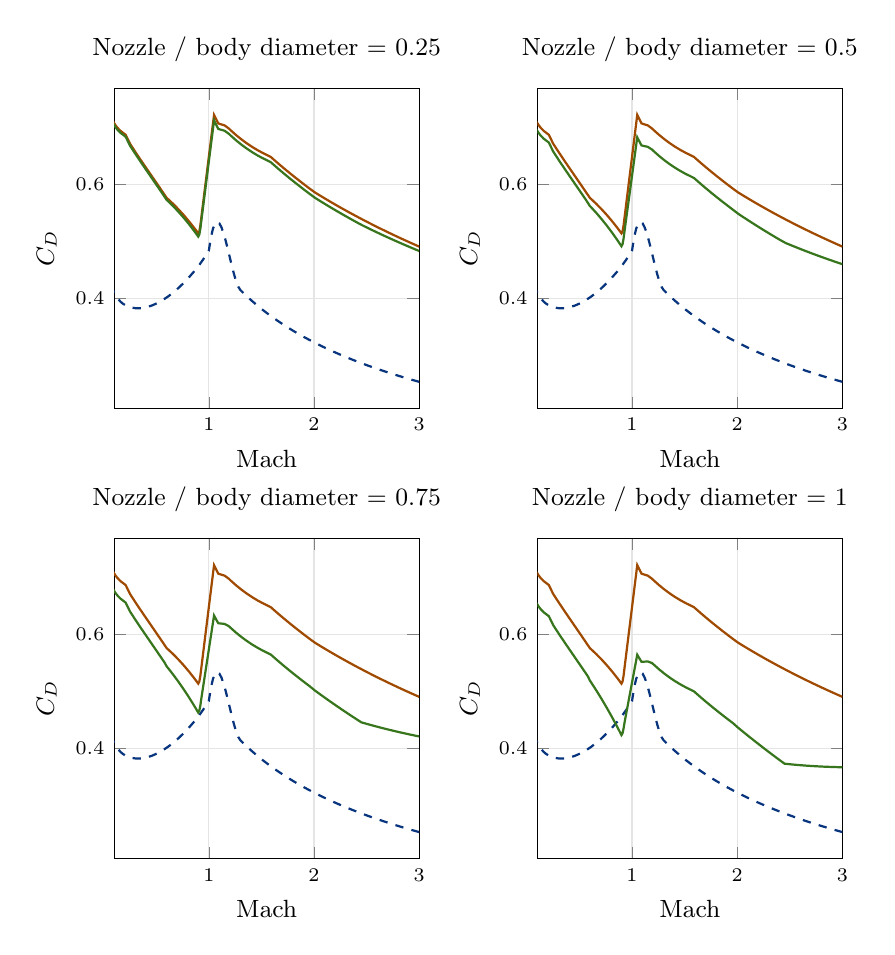
\begin{tikzpicture}
\begin{groupplot}[group style={group size=2 by 2,horizontal sep=1.50cm,vertical sep=1.65cm},width=.45\textwidth,height=5.65cm,grid=major,grid style={gray!20},tick label style={font=\scriptsize},label style={font=\small},title style={font=\small},scaled y ticks=false,yticklabel style={/pgf/number format/fixed,/pgf/number format/precision=3},unbounded coords=jump]
\nextgroupplot[title={Nozzle / body diameter = 0.25},xlabel={Mach},ylabel={$C_D$},xmin=0.1,xmax=3]
\addplot[thick,B,dashed] coordinates {(0.01,0.5392703) (0.02,0.4900503) (0.03,0.4658697) (0.04,0.450449) (0.05,0.4393925) (0.06,0.4309168) (0.07,0.424134) (0.08,0.4185425) (0.09,0.4138331) (0.11,0.4063117) (0.13,0.4005716) (0.16,0.3941944) (0.18,0.3910132) (0.21,0.3874247) (0.23,0.3856667) (0.26,0.3838032) (0.31,0.3823806) (0.36,0.3826665) (0.41,0.3843774) (0.46,0.3873356) (0.51,0.3914235) (0.56,0.3965597) (0.61,0.4026861) (0.66,0.40976) (0.71,0.4177495) (0.76,0.4266305) (0.81,0.4363845) (0.86,0.4469972) (0.91,0.4585945) (0.96,0.4716979) (1,0.4829383) (1.01,0.4948939) (1.02,0.5066529) (1.04,0.5223558) (1.06,0.531185) (1.08,0.5340179) (1.1,0.5317335) (1.11,0.5282184) (1.12,0.5247436) (1.14,0.5143528) (1.16,0.5014411) (1.18,0.4868895) (1.21,0.4639718) (1.22,0.4563939) (1.24,0.442215) (1.26,0.4299264) (1.28,0.420412) (1.3,0.4145561) (1.31,0.4127028) (1.36,0.4037825) (1.41,0.3953943) (1.46,0.3874794) (1.51,0.3799903) (1.56,0.3728856) (1.61,0.3661305) (1.66,0.3596946) (1.71,0.3535516) (1.76,0.3476781) (1.81,0.342054) (1.86,0.3366609) (1.91,0.3314828) (1.96,0.3265051) (2.01,0.321715) (2.06,0.3171006) (2.11,0.3126512) (2.16,0.3083573) (2.21,0.3042101) (2.26,0.3002013) (2.31,0.2963238) (2.36,0.2925705) (2.41,0.2889353) (2.46,0.2854124) (2.51,0.2819964) (2.56,0.2786823) (2.61,0.2754654) (2.66,0.2723414) (2.71,0.2693063) (2.76,0.2663562) (2.81,0.2634875) (2.86,0.2606971) (2.91,0.2579816) (2.96,0.2553382) (3,0.2532734)};
\addplot[thick,burntorange] coordinates {(0.01,0.8080247) (0.02,0.7703703) (0.03,0.7516897) (0.04,0.7397161) (0.05,0.7310909) (0.06,0.7244427) (0.07,0.7190856) (0.08,0.7146313) (0.09,0.71084) (0.11,0.7046646) (0.13,0.6997837) (0.16,0.6940281) (0.21,0.6869798) (0.25,0.6717458) (0.26,0.6688288) (0.31,0.6546548) (0.36,0.6409243) (0.41,0.6274162) (0.46,0.6139917) (0.51,0.6005588) (0.56,0.5870533) (0.6,0.5761646) (0.61,0.5745601) (0.66,0.5659074) (0.71,0.5565273) (0.76,0.5463991) (0.81,0.5355068) (0.86,0.5238373) (0.9,0.5139346) (0.91,0.5174294) (0.92,0.5279136) (0.96,0.5879089) (1.01,0.6623833) (1.05,0.7219628) (1.06,0.7181847) (1.09,0.7070495) (1.11,0.7057831) (1.15,0.7035359) (1.16,0.7021903) (1.19,0.6981246) (1.21,0.6946208) (1.26,0.6864266) (1.31,0.6789658) (1.36,0.6721722) (1.41,0.6659967) (1.46,0.660401) (1.51,0.6553543) (1.56,0.6508322) (1.59,0.6480014) (1.61,0.644709) (1.66,0.6366592) (1.71,0.6288397) (1.76,0.6212208) (1.81,0.6137783) (1.86,0.6064927) (1.91,0.5993475) (1.96,0.5923293) (2.01,0.5856607) (2.06,0.5800016) (2.11,0.5744531) (2.16,0.5690102) (2.21,0.5636688) (2.26,0.5584257) (2.31,0.5532778) (2.36,0.5482225) (2.41,0.5432574) (2.46,0.5383803) (2.51,0.533589) (2.56,0.5288813) (2.61,0.5242552) (2.66,0.5197083) (2.71,0.5152385) (2.76,0.5108433) (2.81,0.5065202) (2.86,0.5022668) (2.91,0.4980803) (2.96,0.4939578) (3,0.4907041)};
\addplot[thick,g] coordinates {(0.01,0.804606) (0.02,0.7669515) (0.03,0.748271) (0.04,0.7362973) (0.05,0.7276722) (0.06,0.7210239) (0.07,0.7156668) (0.08,0.7112126) (0.09,0.7074213) (0.11,0.7012459) (0.13,0.696365) (0.16,0.6906093) (0.21,0.6835611) (0.25,0.668327) (0.26,0.66541) (0.31,0.651236) (0.36,0.6375056) (0.41,0.6239975) (0.46,0.6105729) (0.51,0.5971401) (0.56,0.5836345) (0.6,0.5726067) (0.61,0.5709327) (0.66,0.5619321) (0.71,0.5522041) (0.76,0.5417282) (0.81,0.530488) (0.86,0.5184707) (0.9,0.5082898) (0.91,0.5117461) (0.92,0.5221153) (0.93,0.5371815) (0.96,0.580918) (1.01,0.6538121) (1.05,0.7121274) (1.06,0.708391) (1.09,0.6973807) (1.11,0.6961977) (1.15,0.6941172) (1.16,0.6928132) (1.19,0.6888725) (1.21,0.6853832) (1.26,0.6771891) (1.31,0.6697283) (1.36,0.6629347) (1.41,0.6567592) (1.46,0.6511635) (1.51,0.6461167) (1.56,0.6415947) (1.59,0.6387639) (1.61,0.6354715) (1.66,0.6274217) (1.71,0.6196021) (1.76,0.6119833) (1.81,0.6045408) (1.86,0.5972552) (1.91,0.59011) (1.96,0.5830918) (2.01,0.5763284) (2.06,0.5705508) (2.11,0.5648838) (2.16,0.5593225) (2.21,0.5538626) (2.26,0.5485009) (2.31,0.5432345) (2.36,0.5380608) (2.41,0.5329771) (2.46,0.5280534) (2.51,0.5235031) (2.56,0.5190363) (2.61,0.5146511) (2.66,0.5103451) (2.71,0.5061162) (2.76,0.5019619) (2.81,0.4978798) (2.86,0.4938673) (2.91,0.4899216) (2.96,0.4860401) (3,0.482979)};
\nextgroupplot[title={Nozzle / body diameter = 0.5},xlabel={Mach},ylabel={$C_D$},xmin=0.1,xmax=3]
\addplot[thick,B,dashed] coordinates {(0.01,0.5392703) (0.02,0.4900503) (0.03,0.4658697) (0.04,0.450449) (0.05,0.4393925) (0.06,0.4309168) (0.07,0.424134) (0.08,0.4185425) (0.09,0.4138331) (0.11,0.4063117) (0.13,0.4005716) (0.16,0.3941944) (0.18,0.3910132) (0.21,0.3874247) (0.23,0.3856667) (0.26,0.3838032) (0.31,0.3823806) (0.36,0.3826665) (0.41,0.3843774) (0.46,0.3873356) (0.51,0.3914235) (0.56,0.3965597) (0.61,0.4026861) (0.66,0.40976) (0.71,0.4177495) (0.76,0.4266305) (0.81,0.4363845) (0.86,0.4469972) (0.91,0.4585945) (0.96,0.4716979) (1,0.4829383) (1.01,0.4948939) (1.02,0.5066529) (1.04,0.5223558) (1.06,0.531185) (1.08,0.5340179) (1.1,0.5317335) (1.11,0.5282184) (1.12,0.5247436) (1.14,0.5143528) (1.16,0.5014411) (1.18,0.4868895) (1.21,0.4639718) (1.22,0.4563939) (1.24,0.442215) (1.26,0.4299264) (1.28,0.420412) (1.3,0.4145561) (1.31,0.4127028) (1.36,0.4037825) (1.41,0.3953943) (1.46,0.3874794) (1.51,0.3799903) (1.56,0.3728856) (1.61,0.3661305) (1.66,0.3596946) (1.71,0.3535516) (1.76,0.3476781) (1.81,0.342054) (1.86,0.3366609) (1.91,0.3314828) (1.96,0.3265051) (2.01,0.321715) (2.06,0.3171006) (2.11,0.3126512) (2.16,0.3083573) (2.21,0.3042101) (2.26,0.3002013) (2.31,0.2963238) (2.36,0.2925705) (2.41,0.2889353) (2.46,0.2854124) (2.51,0.2819964) (2.56,0.2786823) (2.61,0.2754654) (2.66,0.2723414) (2.71,0.2693063) (2.76,0.2663562) (2.81,0.2634875) (2.86,0.2606971) (2.91,0.2579816) (2.96,0.2553382) (3,0.2532734)};
\addplot[thick,burntorange] coordinates {(0.01,0.8080247) (0.02,0.7703703) (0.03,0.7516897) (0.04,0.7397161) (0.05,0.7310909) (0.06,0.7244427) (0.07,0.7190856) (0.08,0.7146313) (0.09,0.71084) (0.11,0.7046646) (0.13,0.6997837) (0.16,0.6940281) (0.21,0.6869798) (0.25,0.6717458) (0.26,0.6688288) (0.31,0.6546548) (0.36,0.6409243) (0.41,0.6274162) (0.46,0.6139917) (0.51,0.6005588) (0.56,0.5870533) (0.6,0.5761646) (0.61,0.5745601) (0.66,0.5659074) (0.71,0.5565273) (0.76,0.5463991) (0.81,0.5355068) (0.86,0.5238373) (0.9,0.5139346) (0.91,0.5174294) (0.92,0.5279136) (0.96,0.5879089) (1.01,0.6623833) (1.05,0.7219628) (1.06,0.7181847) (1.09,0.7070495) (1.11,0.7057831) (1.15,0.7035359) (1.16,0.7021903) (1.19,0.6981246) (1.21,0.6946208) (1.26,0.6864266) (1.31,0.6789658) (1.36,0.6721722) (1.41,0.6659967) (1.46,0.660401) (1.51,0.6553543) (1.56,0.6508322) (1.59,0.6480014) (1.61,0.644709) (1.66,0.6366592) (1.71,0.6288397) (1.76,0.6212208) (1.81,0.6137783) (1.86,0.6064927) (1.91,0.5993475) (1.96,0.5923293) (2.01,0.5856607) (2.06,0.5800016) (2.11,0.5744531) (2.16,0.5690102) (2.21,0.5636688) (2.26,0.5584257) (2.31,0.5532778) (2.36,0.5482225) (2.41,0.5432574) (2.46,0.5383803) (2.51,0.533589) (2.56,0.5288813) (2.61,0.5242552) (2.66,0.5197083) (2.71,0.5152385) (2.76,0.5108433) (2.81,0.5065202) (2.86,0.5022668) (2.91,0.4980803) (2.96,0.4939578) (3,0.4907041)};
\addplot[thick,g] coordinates {(0.01,0.7943497) (0.02,0.7566952) (0.03,0.7380147) (0.04,0.726041) (0.05,0.7174159) (0.06,0.7107676) (0.07,0.7054106) (0.08,0.7009563) (0.09,0.697165) (0.11,0.6909896) (0.13,0.6861087) (0.16,0.6803531) (0.21,0.6733048) (0.25,0.6580708) (0.26,0.6551537) (0.31,0.6409798) (0.36,0.6272493) (0.41,0.6137412) (0.46,0.6003166) (0.51,0.5868838) (0.56,0.5733782) (0.6,0.5619331) (0.61,0.5600503) (0.66,0.5500063) (0.71,0.5392348) (0.76,0.5277154) (0.81,0.5154318) (0.86,0.502371) (0.9,0.4913552) (0.91,0.4946965) (0.92,0.5047201) (0.93,0.5190532) (0.96,0.5599451) (1.01,0.6280984) (1.05,0.6826211) (1.06,0.6790097) (1.09,0.6683744) (1.11,0.6674414) (1.15,0.6658609) (1.16,0.6646819) (1.19,0.6611162) (1.21,0.6576707) (1.26,0.6494765) (1.31,0.6420158) (1.36,0.6352222) (1.41,0.6290467) (1.46,0.623451) (1.51,0.6184042) (1.56,0.6138821) (1.59,0.6110514) (1.61,0.6077589) (1.66,0.5997092) (1.71,0.5918896) (1.76,0.5842707) (1.81,0.5768282) (1.86,0.5695426) (1.91,0.5623975) (1.96,0.5553792) (2.01,0.5483315) (2.06,0.5421984) (2.11,0.5361759) (2.16,0.5302591) (2.21,0.5244438) (2.26,0.5187267) (2.31,0.5131048) (2.36,0.5075756) (2.41,0.5021365) (2.46,0.4970729) (2.51,0.4932453) (2.56,0.4895012) (2.61,0.4858387) (2.66,0.4822555) (2.71,0.4787493) (2.76,0.4753178) (2.81,0.4719584) (2.86,0.4686686) (2.91,0.4654457) (2.96,0.4622869) (3,0.459804)};
\nextgroupplot[title={Nozzle / body diameter = 0.75},xlabel={Mach},ylabel={$C_D$},xmin=0.1,xmax=3]
\addplot[thick,B,dashed] coordinates {(0.01,0.5392703) (0.02,0.4900503) (0.03,0.4658697) (0.04,0.450449) (0.05,0.4393925) (0.06,0.4309168) (0.07,0.424134) (0.08,0.4185425) (0.09,0.4138331) (0.11,0.4063117) (0.13,0.4005716) (0.16,0.3941944) (0.18,0.3910132) (0.21,0.3874247) (0.23,0.3856667) (0.26,0.3838032) (0.31,0.3823806) (0.36,0.3826665) (0.41,0.3843774) (0.46,0.3873356) (0.51,0.3914235) (0.56,0.3965597) (0.61,0.4026861) (0.66,0.40976) (0.71,0.4177495) (0.76,0.4266305) (0.81,0.4363845) (0.86,0.4469972) (0.91,0.4585945) (0.96,0.4716979) (1,0.4829383) (1.01,0.4948939) (1.02,0.5066529) (1.04,0.5223558) (1.06,0.531185) (1.08,0.5340179) (1.1,0.5317335) (1.11,0.5282184) (1.12,0.5247436) (1.14,0.5143528) (1.16,0.5014411) (1.18,0.4868895) (1.21,0.4639718) (1.22,0.4563939) (1.24,0.442215) (1.26,0.4299264) (1.28,0.420412) (1.3,0.4145561) (1.31,0.4127028) (1.36,0.4037825) (1.41,0.3953943) (1.46,0.3874794) (1.51,0.3799903) (1.56,0.3728856) (1.61,0.3661305) (1.66,0.3596946) (1.71,0.3535516) (1.76,0.3476781) (1.81,0.342054) (1.86,0.3366609) (1.91,0.3314828) (1.96,0.3265051) (2.01,0.321715) (2.06,0.3171006) (2.11,0.3126512) (2.16,0.3083573) (2.21,0.3042101) (2.26,0.3002013) (2.31,0.2963238) (2.36,0.2925705) (2.41,0.2889353) (2.46,0.2854124) (2.51,0.2819964) (2.56,0.2786823) (2.61,0.2754654) (2.66,0.2723414) (2.71,0.2693063) (2.76,0.2663562) (2.81,0.2634875) (2.86,0.2606971) (2.91,0.2579816) (2.96,0.2553382) (3,0.2532734)};
\addplot[thick,burntorange] coordinates {(0.01,0.8080247) (0.02,0.7703703) (0.03,0.7516897) (0.04,0.7397161) (0.05,0.7310909) (0.06,0.7244427) (0.07,0.7190856) (0.08,0.7146313) (0.09,0.71084) (0.11,0.7046646) (0.13,0.6997837) (0.16,0.6940281) (0.21,0.6869798) (0.25,0.6717458) (0.26,0.6688288) (0.31,0.6546548) (0.36,0.6409243) (0.41,0.6274162) (0.46,0.6139917) (0.51,0.6005588) (0.56,0.5870533) (0.6,0.5761646) (0.61,0.5745601) (0.66,0.5659074) (0.71,0.5565273) (0.76,0.5463991) (0.81,0.5355068) (0.86,0.5238373) (0.9,0.5139346) (0.91,0.5174294) (0.92,0.5279136) (0.96,0.5879089) (1.01,0.6623833) (1.05,0.7219628) (1.06,0.7181847) (1.09,0.7070495) (1.11,0.7057831) (1.15,0.7035359) (1.16,0.7021903) (1.19,0.6981246) (1.21,0.6946208) (1.26,0.6864266) (1.31,0.6789658) (1.36,0.6721722) (1.41,0.6659967) (1.46,0.660401) (1.51,0.6553543) (1.56,0.6508322) (1.59,0.6480014) (1.61,0.644709) (1.66,0.6366592) (1.71,0.6288397) (1.76,0.6212208) (1.81,0.6137783) (1.86,0.6064927) (1.91,0.5993475) (1.96,0.5923293) (2.01,0.5856607) (2.06,0.5800016) (2.11,0.5744531) (2.16,0.5690102) (2.21,0.5636688) (2.26,0.5584257) (2.31,0.5532778) (2.36,0.5482225) (2.41,0.5432574) (2.46,0.5383803) (2.51,0.533589) (2.56,0.5288813) (2.61,0.5242552) (2.66,0.5197083) (2.71,0.5152385) (2.76,0.5108433) (2.81,0.5065202) (2.86,0.5022668) (2.91,0.4980803) (2.96,0.4939578) (3,0.4907041)};
\addplot[thick,g] coordinates {(0.01,0.7772559) (0.02,0.7396015) (0.03,0.7209209) (0.04,0.7089473) (0.05,0.7003221) (0.06,0.6936739) (0.07,0.6883168) (0.08,0.6838625) (0.09,0.6800712) (0.11,0.6738958) (0.13,0.6690149) (0.16,0.6632593) (0.21,0.656211) (0.25,0.640977) (0.26,0.63806) (0.31,0.623886) (0.36,0.6101555) (0.41,0.5966474) (0.46,0.5832229) (0.51,0.56979) (0.56,0.5562845) (0.58,0.550851) (0.6,0.5441436) (0.61,0.541913) (0.66,0.5301299) (0.71,0.5176193) (0.76,0.5043608) (0.81,0.490338) (0.86,0.4755381) (0.9,0.463131) (0.91,0.4662803) (0.92,0.4757282) (0.93,0.4888393) (0.96,0.5249904) (1.01,0.5852424) (1.05,0.6334439) (1.06,0.6300408) (1.09,0.6200306) (1.11,0.6195142) (1.15,0.618767) (1.16,0.6177964) (1.19,0.6148557) (1.21,0.6114831) (1.26,0.6032889) (1.31,0.5958282) (1.36,0.5890346) (1.41,0.5828591) (1.46,0.5772634) (1.51,0.5722166) (1.56,0.5676945) (1.59,0.5648638) (1.61,0.5615714) (1.66,0.5535216) (1.71,0.545702) (1.76,0.5380831) (1.81,0.5306406) (1.86,0.5233551) (1.91,0.5162099) (1.96,0.5091916) (2.01,0.5016699) (2.06,0.4949444) (2.11,0.4883295) (2.16,0.4818202) (2.21,0.4754124) (2.26,0.4691029) (2.31,0.4628885) (2.36,0.4567669) (2.41,0.4507353) (2.45,0.4459737) (2.46,0.4454387) (2.51,0.4428157) (2.56,0.4402762) (2.61,0.4378182) (2.66,0.4354395) (2.71,0.4331379) (2.76,0.4309109) (2.81,0.428756) (2.86,0.4266708) (2.91,0.4246524) (2.96,0.4226982) (3,0.4211789)};
\nextgroupplot[title={Nozzle / body diameter = 1},xlabel={Mach},ylabel={$C_D$},xmin=0.1,xmax=3]
\addplot[thick,B,dashed] coordinates {(0.01,0.5392703) (0.02,0.4900503) (0.03,0.4658697) (0.04,0.450449) (0.05,0.4393925) (0.06,0.4309168) (0.07,0.424134) (0.08,0.4185425) (0.09,0.4138331) (0.11,0.4063117) (0.13,0.4005716) (0.16,0.3941944) (0.18,0.3910132) (0.21,0.3874247) (0.23,0.3856667) (0.26,0.3838032) (0.31,0.3823806) (0.36,0.3826665) (0.41,0.3843774) (0.46,0.3873356) (0.51,0.3914235) (0.56,0.3965597) (0.61,0.4026861) (0.66,0.40976) (0.71,0.4177495) (0.76,0.4266305) (0.81,0.4363845) (0.86,0.4469972) (0.91,0.4585945) (0.96,0.4716979) (1,0.4829383) (1.01,0.4948939) (1.02,0.5066529) (1.04,0.5223558) (1.06,0.531185) (1.08,0.5340179) (1.1,0.5317335) (1.11,0.5282184) (1.12,0.5247436) (1.14,0.5143528) (1.16,0.5014411) (1.18,0.4868895) (1.21,0.4639718) (1.22,0.4563939) (1.24,0.442215) (1.26,0.4299264) (1.28,0.420412) (1.3,0.4145561) (1.31,0.4127028) (1.36,0.4037825) (1.41,0.3953943) (1.46,0.3874794) (1.51,0.3799903) (1.56,0.3728856) (1.61,0.3661305) (1.66,0.3596946) (1.71,0.3535516) (1.76,0.3476781) (1.81,0.342054) (1.86,0.3366609) (1.91,0.3314828) (1.96,0.3265051) (2.01,0.321715) (2.06,0.3171006) (2.11,0.3126512) (2.16,0.3083573) (2.21,0.3042101) (2.26,0.3002013) (2.31,0.2963238) (2.36,0.2925705) (2.41,0.2889353) (2.46,0.2854124) (2.51,0.2819964) (2.56,0.2786823) (2.61,0.2754654) (2.66,0.2723414) (2.71,0.2693063) (2.76,0.2663562) (2.81,0.2634875) (2.86,0.2606971) (2.91,0.2579816) (2.96,0.2553382) (3,0.2532734)};
\addplot[thick,burntorange] coordinates {(0.01,0.8080247) (0.02,0.7703703) (0.03,0.7516897) (0.04,0.7397161) (0.05,0.7310909) (0.06,0.7244427) (0.07,0.7190856) (0.08,0.7146313) (0.09,0.71084) (0.11,0.7046646) (0.13,0.6997837) (0.16,0.6940281) (0.21,0.6869798) (0.25,0.6717458) (0.26,0.6688288) (0.31,0.6546548) (0.36,0.6409243) (0.41,0.6274162) (0.46,0.6139917) (0.51,0.6005588) (0.56,0.5870533) (0.6,0.5761646) (0.61,0.5745601) (0.66,0.5659074) (0.71,0.5565273) (0.76,0.5463991) (0.81,0.5355068) (0.86,0.5238373) (0.9,0.5139346) (0.91,0.5174294) (0.92,0.5279136) (0.96,0.5879089) (1.01,0.6623833) (1.05,0.7219628) (1.06,0.7181847) (1.09,0.7070495) (1.11,0.7057831) (1.15,0.7035359) (1.16,0.7021903) (1.19,0.6981246) (1.21,0.6946208) (1.26,0.6864266) (1.31,0.6789658) (1.36,0.6721722) (1.41,0.6659967) (1.46,0.660401) (1.51,0.6553543) (1.56,0.6508322) (1.59,0.6480014) (1.61,0.644709) (1.66,0.6366592) (1.71,0.6288397) (1.76,0.6212208) (1.81,0.6137783) (1.86,0.6064927) (1.91,0.5993475) (1.96,0.5923293) (2.01,0.5856607) (2.06,0.5800016) (2.11,0.5744531) (2.16,0.5690102) (2.21,0.5636688) (2.26,0.5584257) (2.31,0.5532778) (2.36,0.5482225) (2.41,0.5432574) (2.46,0.5383803) (2.51,0.533589) (2.56,0.5288813) (2.61,0.5242552) (2.66,0.5197083) (2.71,0.5152385) (2.76,0.5108433) (2.81,0.5065202) (2.86,0.5022668) (2.91,0.4980803) (2.96,0.4939578) (3,0.4907041)};
\addplot[thick,g] coordinates {(0.01,0.7533246) (0.02,0.7156702) (0.03,0.6969896) (0.04,0.685016) (0.05,0.6763908) (0.06,0.6697426) (0.07,0.6643855) (0.08,0.6599312) (0.09,0.65614) (0.11,0.6499645) (0.13,0.6450836) (0.16,0.639328) (0.21,0.6322797) (0.25,0.6170457) (0.26,0.6141287) (0.31,0.5999547) (0.36,0.5862242) (0.41,0.5727161) (0.46,0.5592916) (0.51,0.5458588) (0.56,0.5323532) (0.58,0.5269197) (0.6,0.5192384) (0.61,0.5165209) (0.66,0.5023029) (0.71,0.4873576) (0.76,0.4716642) (0.81,0.4552067) (0.86,0.437972) (0.9,0.4236171) (0.91,0.4264977) (0.92,0.4351395) (0.93,0.4465398) (0.96,0.4760538) (1.01,0.5252439) (1.05,0.5645959) (1.06,0.5614845) (1.09,0.5523492) (1.11,0.5524162) (1.15,0.5528357) (1.16,0.5521567) (1.19,0.550091) (1.21,0.5468205) (1.26,0.5386263) (1.31,0.5311656) (1.36,0.524372) (1.41,0.5181965) (1.46,0.5126008) (1.51,0.507554) (1.56,0.5030319) (1.59,0.5002012) (1.61,0.4969088) (1.66,0.488859) (1.71,0.4810394) (1.76,0.4734205) (1.81,0.465978) (1.86,0.4586925) (1.91,0.4515473) (1.96,0.444529) (2.01,0.4363438) (2.06,0.4287889) (2.11,0.4213445) (2.16,0.4140058) (2.21,0.4067686) (2.26,0.3996296) (2.31,0.3925858) (2.36,0.3856348) (2.41,0.3787738) (2.45,0.3733485) (2.46,0.3731509) (2.51,0.3722142) (2.56,0.371361) (2.61,0.3705894) (2.66,0.3698971) (2.71,0.3692819) (2.76,0.3687412) (2.81,0.3682727) (2.86,0.3678739) (2.91,0.3675419) (2.96,0.367274) (3,0.3671039)};
\end{groupplot}\end{tikzpicture}
\caption{Aero-only probes. OR has no corresponding nozzle-area correction here; its baseline is shown to reveal the missing dependency, not as a matched powered-flow prediction.}\label{fig:atlas-21-nozzle-Hsq}
\end{figure}
\noindent{\footnotesize Export files: \code{21-nozzle-Hsq.svg} and \code{21-nozzle-Hsq.png}.\\ Directory: \code{aerodynamic-investigation/extended/figures/}.}

\clearpage\subsubsection*{Test of nozzle-area scaling}
\begin{figure}[H]\centering
{\footnotesize\begin{tabular}{ll}
\tikz[baseline=-.5ex]{\draw[thick,B] (0,0)--(.40,0);}\ Hbody RAS & \tikz[baseline=-.5ex]{\draw[thick,B,dashed] (0,0)--(.40,0);}\ Hbody area-proportional line\\
\tikz[baseline=-.5ex]{\draw[thick,burntorange] (0,0)--(.40,0);}\ Hsq RAS & \tikz[baseline=-.5ex]{\draw[thick,burntorange,dashed] (0,0)--(.40,0);}\ Hsq area-proportional line\\
\end{tabular}}\par\vspace{.7em}
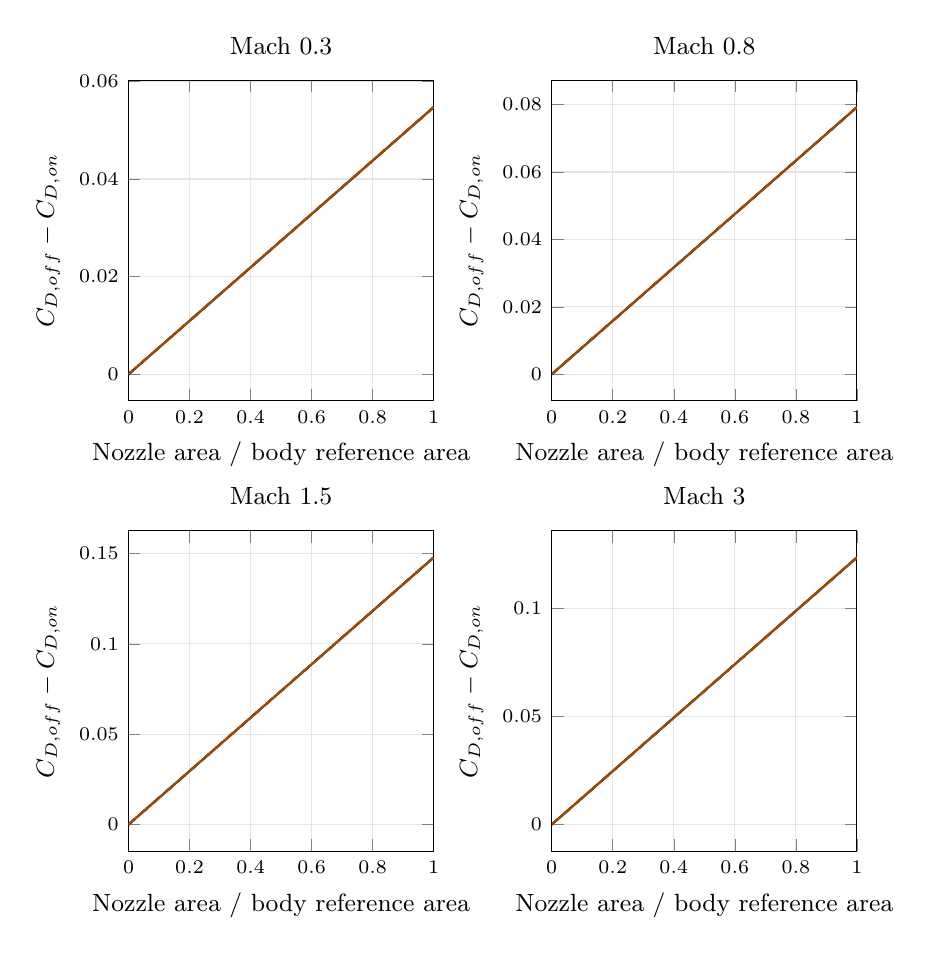
\begin{tikzpicture}
\begin{groupplot}[group style={group size=2 by 2,horizontal sep=1.50cm,vertical sep=1.65cm},width=.45\textwidth,height=5.65cm,grid=major,grid style={gray!20},tick label style={font=\scriptsize},label style={font=\small},title style={font=\small},scaled y ticks=false,yticklabel style={/pgf/number format/fixed,/pgf/number format/precision=3},unbounded coords=jump]
\nextgroupplot[title={Mach 0.3},xlabel={Nozzle area / body reference area},ylabel={$C_{D,off}-C_{D,on}$},xmin=0,xmax=1]
\addplot[thick,B] coordinates {(0,0) (0.0625,0.003418756) (0.25,0.01367502) (0.5625,0.0307688) (1,0.05470009)};
\addplot[thick,B,dashed] coordinates {(0,0) (0.0625,0.003418756) (0.25,0.01367502) (0.5625,0.0307688) (1,0.05470009)};
\addplot[thick,burntorange] coordinates {(0,0) (0.0625,0.003418756) (0.25,0.01367502) (0.5625,0.0307688) (1,0.05470009)};
\addplot[thick,burntorange,dashed] coordinates {(0,0) (0.0625,0.003418756) (0.25,0.01367502) (0.5625,0.0307688) (1,0.05470009)};
\nextgroupplot[title={Mach 0.8},xlabel={Nozzle area / body reference area},ylabel={$C_{D,off}-C_{D,on}$},xmin=0,xmax=1]
\addplot[thick,B] coordinates {(0,0) (0.0625,0.004949193) (0.25,0.01979677) (0.5625,0.04454274) (1,0.07918709)};
\addplot[thick,B,dashed] coordinates {(0,0) (0.0625,0.004949193) (0.25,0.01979677) (0.5625,0.04454274) (1,0.07918709)};
\addplot[thick,burntorange] coordinates {(0,0) (0.0625,0.004949193) (0.25,0.01979677) (0.5625,0.04454274) (1,0.07918709)};
\addplot[thick,burntorange,dashed] coordinates {(0,0) (0.0625,0.004949193) (0.25,0.01979677) (0.5625,0.04454274) (1,0.07918709)};
\nextgroupplot[title={Mach 1.5},xlabel={Nozzle area / body reference area},ylabel={$C_{D,off}-C_{D,on}$},xmin=0,xmax=1]
\addplot[thick,B] coordinates {(0,0) (0.0625,0.009237516) (0.25,0.03695006) (0.5625,0.08313764) (1,0.1478002)};
\addplot[thick,B,dashed] coordinates {(0,0) (0.0625,0.009237516) (0.25,0.03695006) (0.5625,0.08313764) (1,0.1478002)};
\addplot[thick,burntorange] coordinates {(0,0) (0.0625,0.009237516) (0.25,0.03695006) (0.5625,0.08313764) (1,0.1478002)};
\addplot[thick,burntorange,dashed] coordinates {(0,0) (0.0625,0.009237516) (0.25,0.03695006) (0.5625,0.08313764) (1,0.1478002)};
\nextgroupplot[title={Mach 3},xlabel={Nozzle area / body reference area},ylabel={$C_{D,off}-C_{D,on}$},xmin=0,xmax=1]
\addplot[thick,B] coordinates {(0,0) (0.0625,0.007725013) (0.25,0.03090005) (0.5625,0.06952512) (1,0.1236002)};
\addplot[thick,B,dashed] coordinates {(0,0) (0.0625,0.007725013) (0.25,0.03090005) (0.5625,0.06952512) (1,0.1236002)};
\addplot[thick,burntorange] coordinates {(0,0) (0.0625,0.007725013) (0.25,0.03090005) (0.5625,0.06952512) (1,0.1236002)};
\addplot[thick,burntorange,dashed] coordinates {(0,0) (0.0625,0.007725013) (0.25,0.03090005) (0.5625,0.06952512) (1,0.1236002)};
\end{groupplot}\end{tikzpicture}
\caption{The dashed line uses the observed full-area value. It tests area proportionality; it does not identify the absolute body-base coefficient.}\label{fig:atlas-22-nozzle-area-law}
\end{figure}
\noindent{\footnotesize Export files: \code{22-nozzle-area-law.svg} and \code{22-nozzle-area-law.png}.\\ Directory: \code{aerodynamic-investigation/extended/figures/}.}

\clearpage\subsubsection*{Wind-axis drag at 0, 2 and 4 degrees}
\begin{figure}[H]\centering
{\footnotesize\begin{tabular}{lll}
\tikz[baseline=-.5ex]{\draw[thick,B,dashed] (0,0)--(.40,0);}\ MIT OR, 0 deg & \tikz[baseline=-.5ex]{\draw[thick,B] (0,0)--(.40,0);}\ RASAero, 0 deg & \tikz[baseline=-.5ex]{\draw[thick,g,dashed] (0,0)--(.40,0);}\ MIT OR, 2 deg\\
\tikz[baseline=-.5ex]{\draw[thick,g] (0,0)--(.40,0);}\ RASAero, 2 deg & \tikz[baseline=-.5ex]{\draw[thick,burntorange,dashed] (0,0)--(.40,0);}\ MIT OR, 4 deg & \tikz[baseline=-.5ex]{\draw[thick,burntorange] (0,0)--(.40,0);}\ RASAero, 4 deg\\
\end{tabular}}\par\vspace{.7em}
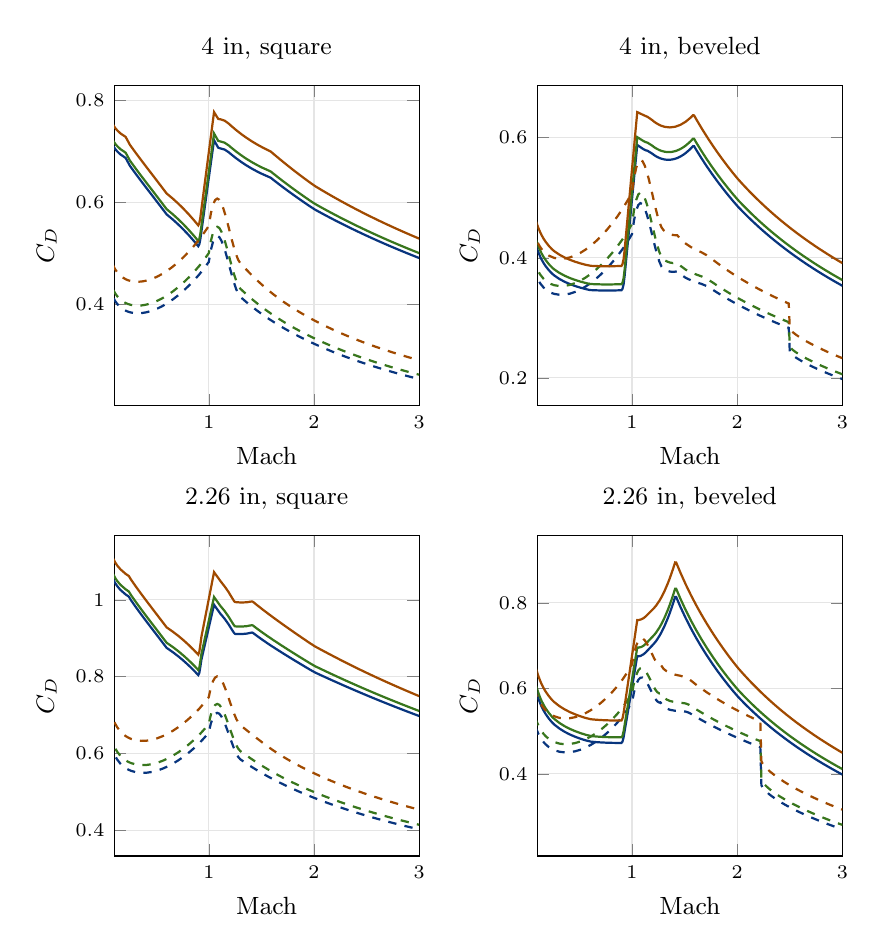
\begin{tikzpicture}
\begin{groupplot}[group style={group size=2 by 2,horizontal sep=1.50cm,vertical sep=1.65cm},width=.45\textwidth,height=5.65cm,grid=major,grid style={gray!20},tick label style={font=\scriptsize},label style={font=\small},title style={font=\small},scaled y ticks=false,yticklabel style={/pgf/number format/fixed,/pgf/number format/precision=3},unbounded coords=jump]
\nextgroupplot[title={4 in, square},xlabel={Mach},ylabel={$C_D$},xmin=0.1,xmax=3]
\addplot[thick,B,dashed] coordinates {(0.01,0.5392703) (0.02,0.4900503) (0.03,0.4658697) (0.04,0.450449) (0.05,0.4393925) (0.06,0.4309168) (0.07,0.424134) (0.08,0.4185425) (0.09,0.4138331) (0.11,0.4063117) (0.13,0.4005716) (0.16,0.3941944) (0.18,0.3910132) (0.21,0.3874247) (0.23,0.3856667) (0.26,0.3838032) (0.31,0.3823806) (0.36,0.3826665) (0.41,0.3843774) (0.46,0.3873356) (0.51,0.3914235) (0.56,0.3965597) (0.61,0.4026861) (0.66,0.40976) (0.71,0.4177495) (0.76,0.4266305) (0.81,0.4363845) (0.86,0.4469972) (0.91,0.4585945) (0.96,0.4716979) (1,0.4829383) (1.01,0.4948939) (1.02,0.5066529) (1.04,0.5223558) (1.06,0.531185) (1.08,0.5340179) (1.1,0.5317335) (1.11,0.5282184) (1.12,0.5247436) (1.14,0.5143528) (1.16,0.5014411) (1.18,0.4868895) (1.21,0.4639718) (1.22,0.4563939) (1.24,0.442215) (1.26,0.4299264) (1.28,0.420412) (1.3,0.4145561) (1.31,0.4127028) (1.36,0.4037825) (1.41,0.3953943) (1.46,0.3874794) (1.51,0.3799903) (1.56,0.3728856) (1.61,0.3661305) (1.66,0.3596946) (1.71,0.3535516) (1.76,0.3476781) (1.81,0.342054) (1.86,0.3366609) (1.91,0.3314828) (1.96,0.3265051) (2.01,0.321715) (2.06,0.3171006) (2.11,0.3126512) (2.16,0.3083573) (2.21,0.3042101) (2.26,0.3002013) (2.31,0.2963238) (2.36,0.2925705) (2.41,0.2889353) (2.46,0.2854124) (2.51,0.2819964) (2.56,0.2786823) (2.61,0.2754654) (2.66,0.2723414) (2.71,0.2693063) (2.76,0.2663562) (2.81,0.2634875) (2.86,0.2606971) (2.91,0.2579816) (2.96,0.2553382) (3,0.2532734)};
\addplot[thick,B] coordinates {(0.01,0.8080247) (0.02,0.7703703) (0.03,0.7516897) (0.04,0.7397161) (0.05,0.7310909) (0.06,0.7244427) (0.07,0.7190856) (0.08,0.7146313) (0.09,0.71084) (0.11,0.7046646) (0.13,0.6997837) (0.16,0.6940281) (0.21,0.6869798) (0.25,0.6717458) (0.26,0.6688288) (0.31,0.6546548) (0.36,0.6409243) (0.41,0.6274162) (0.46,0.6139917) (0.51,0.6005588) (0.56,0.5870533) (0.6,0.5761646) (0.61,0.5745601) (0.66,0.5659074) (0.71,0.5565273) (0.76,0.5463991) (0.81,0.5355068) (0.86,0.5238373) (0.9,0.5139346) (0.91,0.5174294) (0.92,0.5279136) (0.96,0.5879089) (1.01,0.6623833) (1.05,0.7219628) (1.06,0.7181847) (1.09,0.7070495) (1.11,0.7057831) (1.15,0.7035359) (1.16,0.7021903) (1.19,0.6981246) (1.21,0.6946208) (1.26,0.6864266) (1.31,0.6789658) (1.36,0.6721722) (1.41,0.6659967) (1.46,0.660401) (1.51,0.6553543) (1.56,0.6508322) (1.59,0.6480014) (1.61,0.644709) (1.66,0.6366592) (1.71,0.6288397) (1.76,0.6212208) (1.81,0.6137783) (1.86,0.6064927) (1.91,0.5993475) (1.96,0.5923293) (2.01,0.5856607) (2.06,0.5800016) (2.11,0.5744531) (2.16,0.5690102) (2.21,0.5636688) (2.26,0.5584257) (2.31,0.5532778) (2.36,0.5482225) (2.41,0.5432574) (2.46,0.5383803) (2.51,0.533589) (2.56,0.5288813) (2.61,0.5242552) (2.66,0.5197083) (2.71,0.5152385) (2.76,0.5108433) (2.81,0.5065202) (2.86,0.5022668) (2.91,0.4980803) (2.96,0.4939578) (3,0.4907041)};
\addplot[thick,g,dashed] coordinates {(0.01,0.5558584) (0.02,0.5061041) (0.03,0.4816614) (0.04,0.4660738) (0.05,0.4548981) (0.06,0.4463314) (0.07,0.4394763) (0.08,0.4338257) (0.09,0.4290669) (0.11,0.4214678) (0.13,0.4156704) (0.16,0.409233) (0.18,0.4060244) (0.21,0.4024092) (0.23,0.4006414) (0.26,0.3987733) (0.31,0.3973659) (0.36,0.3976916) (0.41,0.399464) (0.46,0.402504) (0.51,0.4066932) (0.56,0.4119497) (0.61,0.4182157) (0.66,0.4254487) (0.71,0.4336175) (0.76,0.442699) (0.81,0.452676) (0.86,0.463536) (0.91,0.4754085) (0.96,0.4888117) (1,0.5002866) (1.01,0.5123964) (1.02,0.5243055) (1.04,0.5402169) (1.06,0.5491698) (1.08,0.5520498) (1.1,0.5497441) (1.11,0.5461875) (1.12,0.542668) (1.14,0.5321394) (1.16,0.5190472) (1.18,0.5042815) (1.21,0.4810006) (1.22,0.4732943) (1.24,0.4588574) (1.26,0.4463159) (1.28,0.4365641) (1.3,0.4304969) (1.31,0.428545) (1.36,0.4190961) (1.41,0.410145) (1.46,0.4016771) (1.51,0.3937074) (1.56,0.3861843) (1.61,0.3790303) (1.66,0.3722613) (1.71,0.3657987) (1.76,0.3596503) (1.81,0.3537612) (1.86,0.3481351) (1.91,0.3427318) (1.96,0.3375529) (2.01,0.3325678) (2.06,0.3277769) (2.11,0.3231563) (2.16,0.318706) (2.21,0.3144065) (2.26,0.3102576) (2.31,0.3062434) (2.36,0.3023637) (2.41,0.298605) (2.46,0.2949671) (2.51,0.2914387) (2.56,0.2880194) (2.61,0.2846996) (2.66,0.2814789) (2.71,0.2783492) (2.76,0.2753098) (2.81,0.2723538) (2.86,0.2694806) (2.91,0.2666841) (2.96,0.2639638) (3,0.261838)};
\addplot[thick,g] coordinates {(0.01,0.8184133) (0.02,0.7807359) (0.03,0.7620439) (0.04,0.750063) (0.05,0.7414326) (0.06,0.7347803) (0.07,0.7294199) (0.08,0.724963) (0.09,0.7211694) (0.11,0.7149902) (0.13,0.7101063) (0.16,0.7043472) (0.21,0.6972946) (0.25,0.6820513) (0.26,0.6791325) (0.31,0.6649499) (0.36,0.651211) (0.41,0.6376947) (0.46,0.624262) (0.51,0.610821) (0.56,0.5973071) (0.6,0.5864118) (0.61,0.5848064) (0.66,0.5761484) (0.71,0.5667625) (0.76,0.5566282) (0.81,0.5457293) (0.86,0.5340527) (0.9,0.5241439) (0.91,0.5278249) (0.92,0.5384997) (0.96,0.599268) (1.01,0.6747084) (1.05,0.7350607) (1.06,0.7313863) (1.09,0.7205203) (1.11,0.7194139) (1.15,0.7170691) (1.16,0.7156876) (1.19,0.7115188) (1.21,0.7079487) (1.26,0.6995968) (1.31,0.6919872) (1.36,0.6850511) (1.41,0.6787379) (1.46,0.6730083) (1.51,0.6678307) (1.56,0.6631801) (1.59,0.6602748) (1.61,0.6569365) (1.66,0.6487574) (1.71,0.640795) (1.76,0.6330262) (1.81,0.6254347) (1.86,0.6180236) (1.91,0.6107539) (1.96,0.6036134) (2.01,0.5968257) (2.06,0.5910514) (2.11,0.5853914) (2.16,0.5798408) (2.21,0.5743955) (2.26,0.5690523) (2.31,0.5638079) (2.36,0.5586631) (2.41,0.5536136) (2.46,0.5486562) (2.51,0.5437886) (2.56,0.5390083) (2.61,0.5343131) (2.66,0.5297006) (2.71,0.5251684) (2.76,0.520714) (2.81,0.5163347) (2.86,0.512028) (2.91,0.5077854) (2.96,0.5036088) (3,0.5003135)};
\addplot[thick,burntorange,dashed] coordinates {(0.01,0.60677) (0.02,0.5556085) (0.03,0.5304755) (0.04,0.514449) (0.05,0.5029597) (0.06,0.494154) (0.07,0.4871088) (0.08,0.4813028) (0.09,0.4764146) (0.11,0.4686128) (0.13,0.4626661) (0.16,0.4560735) (0.18,0.4527952) (0.21,0.4491142) (0.23,0.447324) (0.26,0.4454494) (0.31,0.4440933) (0.36,0.4445371) (0.41,0.4464873) (0.46,0.4497608) (0.51,0.4542372) (0.56,0.4598343) (0.61,0.4664944) (0.66,0.4741763) (0.71,0.4828511) (0.76,0.4924985) (0.81,0.5031053) (0.86,0.5146644) (0.91,0.5273158) (0.96,0.5415691) (1,0.5537129) (1.01,0.5662416) (1.02,0.5785588) (1.04,0.5950453) (1.06,0.6043495) (1.08,0.6073781) (1.1,0.60504) (1.11,0.6013853) (1.12,0.5977591) (1.14,0.5868881) (1.16,0.573339) (1.18,0.5580254) (1.21,0.5338068) (1.22,0.5257669) (1.24,0.5106569) (1.26,0.4974523) (1.28,0.487074) (1.3,0.4804449) (1.31,0.4782286) (1.36,0.4673479) (1.41,0.4568445) (1.46,0.4468198) (1.51,0.4374399) (1.56,0.4285962) (1.61,0.4201874) (1.66,0.4123959) (1.71,0.4049545) (1.76,0.3979763) (1.81,0.3912889) (1.86,0.384968) (1.91,0.3788937) (1.96,0.3731199) (2.01,0.3675585) (2.06,0.3622495) (2.11,0.3571257) (2.16,0.352218) (2.21,0.3474737) (2.26,0.3429169) (2.31,0.3385053) (2.36,0.3342585) (2.41,0.3301417) (2.46,0.3261711) (2.51,0.3223177) (2.56,0.318595) (2.61,0.3149785) (2.66,0.3114796) (2.71,0.3080776) (2.76,0.3047819) (2.81,0.3015749) (2.86,0.2984646) (2.91,0.2954358) (2.96,0.2924953) (3,0.2901949)};
\addplot[thick,burntorange] coordinates {(0.01,0.8495579) (0.02,0.8118115) (0.03,0.7930853) (0.04,0.7810824) (0.05,0.7724362) (0.06,0.7657717) (0.07,0.7604016) (0.08,0.7559364) (0.09,0.7521359) (0.11,0.7459454) (0.13,0.7410526) (0.16,0.7352829) (0.21,0.7282174) (0.25,0.7129462) (0.26,0.710022) (0.31,0.6958134) (0.36,0.6820494) (0.41,0.6685083) (0.46,0.655051) (0.51,0.6415854) (0.56,0.6280468) (0.6,0.6171316) (0.61,0.6155232) (0.66,0.6068493) (0.71,0.5974463) (0.76,0.5872934) (0.81,0.5763745) (0.86,0.5646765) (0.9,0.5547496) (0.91,0.559164) (0.92,0.570585) (0.96,0.6343711) (1.01,0.7135828) (1.05,0.7769522) (1.06,0.7735887) (1.09,0.7635297) (1.11,0.7629026) (1.15,0.7602653) (1.16,0.7587765) (1.19,0.7542984) (1.21,0.7505294) (1.26,0.741705) (1.31,0.733649) (1.36,0.7262857) (1.41,0.7195599) (1.46,0.7133778) (1.51,0.707711) (1.56,0.7025785) (1.59,0.6993915) (1.61,0.6958768) (1.66,0.6872133) (1.71,0.6787261) (1.76,0.6704108) (1.81,0.6622758) (1.86,0.6543916) (1.91,0.646652) (1.96,0.6390482) (2.01,0.6318066) (2.06,0.6255902) (2.11,0.6194991) (2.16,0.6135289) (2.21,0.6076753) (2.26,0.601935) (2.31,0.5963047) (2.36,0.5907947) (2.41,0.5853956) (2.46,0.5801008) (2.51,0.5749075) (2.56,0.5698126) (2.61,0.5648136) (2.66,0.5599076) (2.71,0.5550917) (2.76,0.550363) (2.81,0.5457183) (2.86,0.5411547) (2.91,0.5366689) (2.96,0.5322575) (3,0.5287798)};
\nextgroupplot[title={4 in, beveled},xlabel={Mach},ylabel={$C_D$},xmin=0.1,xmax=3]
\addplot[thick,B,dashed] coordinates {(0.01,0.4955621) (0.02,0.4463415) (0.03,0.4221597) (0.04,0.4067373) (0.05,0.3956786) (0.06,0.3872002) (0.07,0.3804143) (0.08,0.3748193) (0.09,0.3701059) (0.11,0.3625749) (0.13,0.3568235) (0.16,0.3504259) (0.18,0.3472289) (0.21,0.3436136) (0.23,0.3418356) (0.26,0.3399392) (0.31,0.3384548) (0.36,0.3386713) (0.41,0.3403069) (0.46,0.3431862) (0.51,0.3471947) (0.56,0.3522544) (0.61,0.3583117) (0.66,0.3653296) (0.71,0.3732834) (0.76,0.3821579) (0.81,0.3919458) (0.86,0.4026476) (0.91,0.4144078) (0.96,0.4277726) (1,0.4393144) (1.01,0.4510799) (1.02,0.4629209) (1.04,0.4788217) (1.06,0.4878998) (1.08,0.4910396) (1.1,0.4891272) (1.11,0.4858248) (1.12,0.4825817) (1.14,0.4727157) (1.16,0.4604176) (1.18,0.4465782) (1.21,0.4249381) (1.22,0.4178484) (1.24,0.404751) (1.26,0.3936996) (1.28,0.3856) (1.3,0.3813638) (1.31,0.3804075) (1.34,0.37809) (1.36,0.3770685) (1.39,0.3764987) (1.41,0.376916) (1.43,0.3775066) (1.46,0.3727592) (1.51,0.366726) (1.56,0.3625256) (1.61,0.3594235) (1.66,0.3565539) (1.71,0.3529445) (1.76,0.3476781) (1.81,0.342054) (1.86,0.3366609) (1.91,0.3314828) (1.96,0.3265051) (2.01,0.321715) (2.06,0.3171006) (2.11,0.3126512) (2.16,0.3083573) (2.21,0.3042101) (2.26,0.3002013) (2.31,0.2963238) (2.36,0.2925705) (2.41,0.2889353) (2.46,0.2854124) (2.49,0.2833503) (2.5,0.2430483) (2.51,0.240604) (2.53,0.2374095) (2.56,0.233615) (2.61,0.2282684) (2.66,0.2235344) (2.71,0.2191793) (2.76,0.2151014) (2.81,0.2112445) (2.86,0.2075729) (2.91,0.2040619) (2.96,0.2006932) (3,0.1980912)};
\addplot[thick,B] coordinates {(0.01,0.5863164) (0.02,0.5211986) (0.03,0.4891801) (0.04,0.4687447) (0.05,0.4540613) (0.06,0.442762) (0.07,0.4336675) (0.08,0.4261116) (0.09,0.4196841) (0.1,0.4141154) (0.11,0.4092202) (0.13,0.4009531) (0.14,0.3974088) (0.16,0.3912058) (0.18,0.3859236) (0.21,0.3792669) (0.24,0.3737261) (0.26,0.3706882) (0.31,0.3647434) (0.36,0.3600281) (0.41,0.3561808) (0.46,0.3529754) (0.51,0.3502616) (0.56,0.3479347) (0.6,0.3463006) (0.61,0.3462077) (0.66,0.3458135) (0.71,0.3455966) (0.76,0.3455285) (0.81,0.3455865) (0.86,0.3457523) (0.9,0.3459527) (0.91,0.3483052) (0.92,0.3553626) (0.93,0.3697444) (0.96,0.4242766) (1.01,0.5151636) (1.05,0.5878732) (1.06,0.5866429) (1.11,0.5807182) (1.13,0.5790303) (1.15,0.5780496) (1.16,0.576851) (1.19,0.5736579) (1.21,0.5710699) (1.23,0.5688669) (1.26,0.5662524) (1.28,0.564955) (1.31,0.5636602) (1.33,0.5632242) (1.36,0.5632031) (1.38,0.5636076) (1.41,0.5648392) (1.43,0.5660756) (1.46,0.5685528) (1.49,0.5717779) (1.51,0.5743443) (1.54,0.5788208) (1.56,0.5822248) (1.58,0.5859661) (1.59,0.5858598) (1.61,0.5799547) (1.66,0.5658094) (1.71,0.5524506) (1.76,0.5397811) (1.81,0.5277226) (1.86,0.5162118) (1.91,0.5051956) (1.96,0.4946296) (2.01,0.4846276) (2.06,0.475588) (2.11,0.4669043) (2.16,0.4585525) (2.21,0.4505112) (2.26,0.4427617) (2.31,0.4352867) (2.36,0.4280706) (2.41,0.4210989) (2.46,0.4143585) (2.51,0.4078372) (2.56,0.4015231) (2.61,0.3954055) (2.66,0.3894743) (2.71,0.3837197) (2.76,0.3781323) (2.81,0.3727032) (2.86,0.3674241) (2.91,0.3622866) (2.96,0.3572828) (3,0.3533708)};
\addplot[thick,g,dashed] coordinates {(0.01,0.5116754) (0.02,0.4619204) (0.03,0.4374764) (0.04,0.4218872) (0.05,0.4107093) (0.06,0.40214) (0.07,0.3952817) (0.08,0.3896274) (0.09,0.3848646) (0.11,0.3772559) (0.13,0.371447) (0.16,0.364989) (0.18,0.3617644) (0.21,0.3581221) (0.23,0.3563341) (0.26,0.3544328) (0.31,0.3529629) (0.36,0.3532184) (0.41,0.3549147) (0.46,0.357875) (0.51,0.3619839) (0.56,0.3671631) (0.61,0.3733592) (0.66,0.3805357) (0.71,0.3886684) (0.76,0.3977433) (0.81,0.4077546) (0.86,0.4187046) (0.91,0.4307417) (0.96,0.4444092) (1,0.4561889) (1.01,0.4681064) (1.02,0.4800984) (1.04,0.4962099) (1.06,0.5054144) (1.08,0.5086046) (1.1,0.5066749) (1.11,0.5033333) (1.12,0.5000481) (1.14,0.4900499) (1.16,0.4775781) (1.18,0.4635323) (1.21,0.4415429) (1.22,0.4343301) (1.24,0.4209864) (1.26,0.4096956) (1.28,0.401374) (1.3,0.396944) (1.31,0.3958988) (1.34,0.3933039) (1.36,0.3920918) (1.39,0.3912351) (1.41,0.391466) (1.43,0.3918727) (1.46,0.3867971) (1.51,0.380299) (1.56,0.3757118) (1.61,0.3722504) (1.66,0.3690865) (1.71,0.3651851) (1.76,0.3596503) (1.81,0.3537612) (1.86,0.3481351) (1.91,0.3427318) (1.96,0.3375529) (2.01,0.3325678) (2.06,0.3277769) (2.11,0.3231563) (2.16,0.318706) (2.21,0.3144065) (2.26,0.3102576) (2.31,0.3062434) (2.36,0.3023637) (2.41,0.298605) (2.46,0.2949671) (2.49,0.2928365) (2.5,0.2520813) (2.51,0.2495966) (2.53,0.2463398) (2.56,0.2424625) (2.61,0.2369899) (2.66,0.2321417) (2.71,0.2276776) (2.76,0.2234983) (2.81,0.2195433) (2.86,0.2157794) (2.91,0.2121786) (2.96,0.2087251) (3,0.2060563)};
\addplot[thick,g] coordinates {(0.01,0.5965698) (0.02,0.5314123) (0.03,0.4993743) (0.04,0.4789265) (0.05,0.4642341) (0.06,0.4529279) (0.07,0.4438279) (0.08,0.4362674) (0.09,0.4298359) (0.1,0.4242639) (0.11,0.4193657) (0.13,0.4110936) (0.14,0.4075471) (0.16,0.4013403) (0.18,0.3960548) (0.21,0.3893941) (0.24,0.3838499) (0.26,0.3808102) (0.31,0.3748618) (0.36,0.3701436) (0.41,0.3662939) (0.46,0.3630866) (0.51,0.3603711) (0.56,0.3580429) (0.6,0.3564077) (0.61,0.3563148) (0.66,0.3559203) (0.71,0.3557033) (0.76,0.3556352) (0.81,0.3556931) (0.86,0.3558591) (0.9,0.3560596) (0.91,0.3585976) (0.92,0.3658435) (0.93,0.3804182) (0.96,0.435536) (1.01,0.527399) (1.05,0.6008894) (1.06,0.5997643) (1.11,0.5942727) (1.13,0.5925602) (1.15,0.5915063) (1.16,0.590272) (1.19,0.5869763) (1.21,0.5843225) (1.23,0.5820558) (1.26,0.5793494) (1.28,0.5779926) (1.31,0.5766113) (1.33,0.576119) (1.36,0.5760155) (1.38,0.5763663) (1.41,0.5775187) (1.43,0.5787033) (1.46,0.5811042) (1.49,0.5842542) (1.51,0.5867713) (1.54,0.591175) (1.56,0.594531) (1.58,0.5982247) (1.59,0.5980953) (1.61,0.5921427) (1.66,0.5778644) (1.71,0.5643594) (1.76,0.5515368) (1.81,0.5393265) (1.86,0.5276876) (1.91,0.5165446) (1.96,0.5058542) (2.01,0.495731) (2.06,0.4865742) (2.11,0.477777) (2.16,0.4693157) (2.21,0.4611689) (2.26,0.4533178) (2.31,0.4457449) (2.36,0.4384379) (2.41,0.4313807) (2.46,0.4245589) (2.51,0.4179601) (2.56,0.4115724) (2.61,0.4053849) (2.66,0.3993872) (2.71,0.3935695) (2.76,0.3879221) (2.81,0.3824362) (2.86,0.3771031) (2.91,0.3719089) (2.96,0.3668504) (3,0.3628966)};
\addplot[thick,burntorange,dashed] coordinates {(0.01,0.5613366) (0.02,0.5101743) (0.03,0.4850401) (0.04,0.4690118) (0.05,0.4575203) (0.06,0.4487118) (0.07,0.4416634) (0.08,0.4358537) (0.09,0.4309613) (0.11,0.4231496) (0.13,0.4171912) (0.16,0.4105773) (0.18,0.4072826) (0.21,0.4035737) (0.26,0.399854) (0.31,0.3984336) (0.36,0.3988052) (0.41,0.4006771) (0.46,0.4038687) (0.51,0.4082626) (0.56,0.4137802) (0.61,0.4203684) (0.66,0.4279922) (0.71,0.4366298) (0.76,0.4462704) (0.81,0.4569125) (0.86,0.4685642) (0.91,0.4813849) (0.96,0.4959099) (1,0.5083671) (1.01,0.5206981) (1.02,0.5331006) (1.04,0.5497928) (1.06,0.5593557) (1.08,0.5627033) (1.1,0.5607519) (1.11,0.5573183) (1.12,0.553933) (1.14,0.5436075) (1.16,0.5306963) (1.18,0.5161229) (1.21,0.4932323) (1.22,0.4856999) (1.24,0.4717142) (1.26,0.4597955) (1.28,0.450888) (1.3,0.4459424) (1.31,0.4446585) (1.36,0.4395794) (1.39,0.4379286) (1.41,0.4376369) (1.43,0.4375225) (1.46,0.4315186) (1.51,0.4236521) (1.56,0.4178273) (1.61,0.4132157) (1.66,0.4091312) (1.71,0.4043235) (1.76,0.3979763) (1.81,0.3912889) (1.86,0.384968) (1.91,0.3788937) (1.96,0.3731199) (2.01,0.3675585) (2.06,0.3622495) (2.11,0.3571257) (2.16,0.352218) (2.21,0.3474737) (2.26,0.3429169) (2.31,0.3385053) (2.36,0.3342585) (2.41,0.3301417) (2.46,0.3261711) (2.49,0.3238424) (2.5,0.2818878) (2.51,0.2792915) (2.53,0.2758598) (2.56,0.2717488) (2.61,0.2659186) (2.66,0.260746) (2.71,0.255972) (2.76,0.251504) (2.81,0.2472697) (2.86,0.2432435) (2.91,0.2393876) (2.96,0.2356933) (3,0.2328345)};
\addplot[thick,burntorange] coordinates {(0.01,0.6273081) (0.02,0.5620313) (0.03,0.5299347) (0.04,0.5094494) (0.05,0.4947301) (0.06,0.4834032) (0.07,0.4742865) (0.08,0.4667122) (0.09,0.4602689) (0.1,0.4546867) (0.11,0.4497795) (0.13,0.4414923) (0.14,0.4379393) (0.16,0.4317212) (0.18,0.426426) (0.21,0.4197531) (0.24,0.4141987) (0.26,0.4111535) (0.31,0.4051941) (0.36,0.4004673) (0.41,0.3966106) (0.46,0.3933974) (0.51,0.3906769) (0.56,0.3883444) (0.61,0.3866132) (0.66,0.386218) (0.71,0.3860006) (0.76,0.3859323) (0.81,0.3859904) (0.86,0.3861566) (0.9,0.3863575) (0.91,0.3896268) (0.92,0.3976126) (0.93,0.4129406) (0.96,0.4703392) (1.01,0.5660036) (1.05,0.6425351) (1.06,0.6417257) (1.11,0.6375322) (1.15,0.6344726) (1.16,0.6331312) (1.19,0.6295278) (1.21,0.6266769) (1.23,0.6242195) (1.26,0.6212374) (1.28,0.6197026) (1.31,0.6180618) (1.36,0.6170504) (1.41,0.6181553) (1.46,0.6213053) (1.51,0.6265032) (1.56,0.6338036) (1.58,0.6373163) (1.59,0.6370982) (1.61,0.6309644) (1.66,0.6161905) (1.71,0.6021505) (1.76,0.5887722) (1.81,0.5760099) (1.86,0.5638902) (1.91,0.5522702) (1.96,0.54111) (2.01,0.5305267) (2.06,0.5209216) (2.11,0.5116877) (2.16,0.5028014) (2.21,0.4942413) (2.26,0.4859886) (2.31,0.4780255) (2.36,0.4703494) (2.41,0.4629389) (2.46,0.4557762) (2.51,0.4488485) (2.56,0.4421434) (2.61,0.4356494) (2.66,0.4293556) (2.71,0.4232517) (2.76,0.4173279) (2.81,0.4115746) (2.86,0.4059827) (2.91,0.4005436) (2.96,0.3952487) (3,0.3911112)};
\nextgroupplot[title={2.26 in, square},xlabel={Mach},ylabel={$C_D$},xmin=0.1,xmax=3]
\addplot[thick,B,dashed] coordinates {(0.01,0.8020017) (0.02,0.7245741) (0.03,0.686642) (0.04,0.6624746) (0.05,0.6451456) (0.06,0.6318502) (0.07,0.6211938) (0.08,0.6123893) (0.09,0.604952) (0.1,0.5985638) (0.11,0.5930054) (0.13,0.5837918) (0.16,0.5733641) (0.18,0.5680205) (0.21,0.5617585) (0.23,0.5585117) (0.26,0.5547559) (0.31,0.5508767) (0.36,0.549358) (0.41,0.5497589) (0.46,0.5518042) (0.51,0.5553118) (0.56,0.5601566) (0.61,0.5662493) (0.66,0.5735252) (0.71,0.5819362) (0.76,0.5914465) (0.81,0.602029) (0.86,0.6136636) (0.91,0.6265437) (0.96,0.6414652) (1,0.654376) (1.01,0.6666112) (1.02,0.6783271) (1.04,0.6939761) (1.06,0.7027898) (1.08,0.7056421) (1.1,0.7034092) (1.11,0.6998117) (1.12,0.696256) (1.14,0.6857068) (1.16,0.6726397) (1.18,0.6579336) (1.21,0.634783) (1.24,0.6127886) (1.26,0.6003375) (1.28,0.5906565) (1.3,0.5846293) (1.31,0.5826885) (1.36,0.573312) (1.41,0.5644364) (1.46,0.5560049) (1.51,0.547972) (1.56,0.5402991) (1.61,0.5329543) (1.66,0.5259098) (1.71,0.5191422) (1.76,0.5126306) (1.81,0.5063573) (1.86,0.5003061) (1.91,0.494463) (1.96,0.4888153) (2.01,0.4833517) (2.06,0.478062) (2.11,0.4729368) (2.16,0.4679677) (2.21,0.463147) (2.26,0.4584675) (2.31,0.4539226) (2.36,0.4495064) (2.41,0.4452132) (2.46,0.4410376) (2.51,0.436975) (2.56,0.4330207) (2.61,0.4291704) (2.66,0.4254201) (2.71,0.4217661) (2.76,0.4182047) (2.81,0.4147327) (2.86,0.4113467) (2.91,0.4080438) (2.96,0.4048212) (3,0.4022989)};
\addplot[thick,B] coordinates {(0.01,1.21345) (0.02,1.15217) (0.03,1.121582) (0.04,1.101885) (0.05,1.087644) (0.06,1.076632) (0.07,1.067733) (0.08,1.060314) (0.09,1.053986) (0.11,1.043646) (0.13,1.035442) (0.16,1.02573) (0.21,1.01377) (0.24,1.008194) (0.26,0.9992) (0.31,0.9796375) (0.36,0.9609273) (0.41,0.9427009) (0.46,0.9247262) (0.51,0.9068487) (0.56,0.8889601) (0.6,0.8745881) (0.61,0.8728513) (0.66,0.8632907) (0.71,0.8528037) (0.76,0.8413554) (0.81,0.828918) (0.86,0.8154694) (0.9,0.8039702) (0.91,0.8094372) (0.92,0.8258382) (0.93,0.8440995) (0.96,0.8798626) (1.01,0.9394678) (1.05,0.987152) (1.06,0.9829413) (1.11,0.9638933) (1.15,0.9508898) (1.16,0.9469838) (1.19,0.9354468) (1.21,0.9264695) (1.24,0.9136873) (1.25,0.911202) (1.26,0.9109504) (1.31,0.9106605) (1.36,0.9119237) (1.41,0.9146808) (1.42,0.9137596) (1.46,0.905556) (1.51,0.8957788) (1.56,0.8864102) (1.61,0.8773532) (1.66,0.8685357) (1.71,0.8599042) (1.76,0.8514182) (1.81,0.8430476) (1.86,0.8347701) (1.91,0.8265688) (1.96,0.8184316) (2.01,0.8106998) (2.06,0.8043691) (2.11,0.7981008) (2.16,0.7918947) (2.21,0.785751) (2.26,0.7796708) (2.31,0.7736552) (2.36,0.7677052) (2.41,0.7618215) (2.46,0.7560053) (2.51,0.7502567) (2.56,0.7445758) (2.61,0.7389624) (2.66,0.7334156) (2.71,0.7279346) (2.76,0.7225177) (2.81,0.7171629) (2.86,0.7118681) (2.91,0.7066306) (2.96,0.7014473) (3,0.6973375)};
\addplot[thick,g,dashed] coordinates {(0.01,0.8247515) (0.02,0.7464831) (0.03,0.7081395) (0.04,0.6837103) (0.05,0.666194) (0.06,0.6527554) (0.07,0.6419846) (0.08,0.6330861) (0.09,0.6255698) (0.1,0.6191142) (0.11,0.6134978) (0.13,0.6041893) (0.16,0.5936577) (0.18,0.5882635) (0.21,0.5819462) (0.23,0.5786738) (0.26,0.5748933) (0.31,0.5710037) (0.36,0.5695062) (0.41,0.5699555) (0.46,0.5720735) (0.51,0.5756767) (0.56,0.5806388) (0.61,0.5868704) (0.66,0.5943063) (0.71,0.6028988) (0.76,0.6126123) (0.81,0.6234206) (0.86,0.6353043) (0.91,0.6484603) (0.96,0.6636895) (1,0.6768517) (1.01,0.6892455) (1.02,0.7011133) (1.04,0.7169773) (1.06,0.7259253) (1.08,0.7288393) (1.1,0.726604) (1.11,0.7229747) (1.12,0.7193849) (1.14,0.708722) (1.16,0.6955017) (1.18,0.680612) (1.21,0.6571483) (1.24,0.6348209) (1.26,0.6221532) (1.28,0.6122704) (1.3,0.6060659) (1.31,0.6040423) (1.36,0.5942006) (1.41,0.584781) (1.46,0.5757435) (1.51,0.5670791) (1.56,0.5588105) (1.61,0.5508971) (1.66,0.5433809) (1.71,0.5361602) (1.76,0.5292607) (1.81,0.5226131) (1.86,0.5162343) (1.91,0.510074) (1.96,0.504144) (2.01,0.4984064) (2.06,0.4928696) (2.11,0.4875042) (2.16,0.4823162) (2.21,0.4772822) (2.26,0.4724067) (2.31,0.4676707) (2.36,0.4630777) (2.41,0.4586117) (2.46,0.4542756) (2.51,0.4500558) (2.56,0.4459546) (2.61,0.4419606) (2.66,0.4380753) (2.71,0.4342891) (2.76,0.4306031) (2.81,0.4270089) (2.86,0.4235074) (2.91,0.4200913) (2.96,0.4167612) (3,0.4141537)};
\addplot[thick,g] coordinates {(0.01,1.226998) (0.02,1.165681) (0.03,1.135073) (0.04,1.115365) (0.05,1.101115) (0.06,1.090096) (0.07,1.081191) (0.08,1.073769) (0.09,1.067436) (0.11,1.05709) (0.13,1.048881) (0.16,1.039163) (0.21,1.027195) (0.24,1.021616) (0.26,1.012617) (0.31,0.9930426) (0.36,0.974321) (0.41,0.9560834) (0.46,0.9380978) (0.51,0.9202094) (0.56,0.9023099) (0.6,0.8879291) (0.61,0.8861913) (0.66,0.8766248) (0.71,0.8661315) (0.76,0.8546762) (0.81,0.8422312) (0.86,0.8287744) (0.9,0.8172682) (0.91,0.8231921) (0.92,0.8400567) (0.93,0.8587827) (0.96,0.8959284) (1.01,0.957838) (1.05,1.007366) (1.06,1.003257) (1.11,0.9841986) (1.15,0.9710181) (1.16,0.9670702) (1.19,0.9554132) (1.21,0.9463588) (1.24,0.9334655) (1.25,0.9309453) (1.26,0.9306605) (1.31,0.9302111) (1.36,0.9313233) (1.41,0.9339363) (1.42,0.9329868) (1.46,0.9246525) (1.51,0.9146759) (1.56,0.9050791) (1.61,0.8957755) (1.66,0.8867006) (1.71,0.8778065) (1.76,0.8690568) (1.81,0.8604243) (1.86,0.8518886) (1.91,0.8434342) (1.96,0.8350498) (2.01,0.8270775) (2.06,0.820514) (2.11,0.8140199) (2.16,0.8075951) (2.21,0.8012396) (2.26,0.7949544) (2.31,0.7887405) (2.36,0.7825986) (2.41,0.7765294) (2.46,0.7705447) (2.51,0.7646397) (2.56,0.7588078) (2.61,0.7530487) (2.66,0.7473613) (2.71,0.7417445) (2.76,0.7361963) (2.81,0.7307147) (2.86,0.7252973) (2.91,0.7199328) (2.96,0.7146255) (3,0.710419)};
\addplot[thick,burntorange,dashed] coordinates {(0.01,0.8946718) (0.02,0.8141892) (0.03,0.774762) (0.04,0.7496437) (0.05,0.7316345) (0.06,0.717819) (0.07,0.7067476) (0.08,0.6976021) (0.09,0.6898785) (0.11,0.6774776) (0.13,0.6679211) (0.16,0.6571194) (0.18,0.6515945) (0.21,0.6451364) (0.23,0.6418) (0.26,0.6379607) (0.31,0.634055) (0.36,0.6326271) (0.41,0.6332196) (0.46,0.6355476) (0.51,0.6394233) (0.56,0.6447183) (0.61,0.6513418) (0.66,0.6592287) (0.71,0.6683317) (0.76,0.6786169) (0.81,0.69006) (0.86,0.7026445) (0.91,0.7165768) (0.96,0.7326736) (1,0.7465538) (1.01,0.759381) (1.02,0.7716649) (1.04,0.7881295) (1.06,0.797468) (1.08,0.8005841) (1.1,0.798384) (1.11,0.7946924) (1.12,0.7910349) (1.14,0.780117) (1.16,0.7665392) (1.18,0.7512114) (1.21,0.7269912) (1.24,0.7038515) (1.26,0.690653) (1.28,0.6802751) (1.3,0.6736352) (1.31,0.6714077) (1.36,0.6603849) (1.41,0.6495222) (1.46,0.6388059) (1.51,0.6282816) (1.56,0.6181158) (1.61,0.6083982) (1.66,0.5994216) (1.71,0.5908014) (1.76,0.582722) (1.81,0.5749378) (1.86,0.5675743) (1.91,0.5604617) (1.96,0.5536906) (2.01,0.5471371) (2.06,0.5408691) (2.11,0.5347927) (2.16,0.5289603) (2.21,0.5232985) (2.26,0.5178489) (2.31,0.5125527) (2.36,0.5074434) (2.41,0.502473) (2.46,0.4976692) (2.51,0.492992) (2.56,0.4884644) (2.61,0.4840529) (2.66,0.4797768) (2.71,0.4756075) (2.76,0.4715615) (2.81,0.4676142) (2.86,0.4637798) (2.91,0.4600369) (2.96,0.4563977) (3,0.4535445)};
\addplot[thick,burntorange] coordinates {(0.01,1.267614) (0.02,1.206184) (0.03,1.175521) (0.04,1.155777) (0.05,1.1415) (0.06,1.130461) (0.07,1.12154) (0.08,1.114104) (0.09,1.10776) (0.11,1.097395) (0.13,1.089171) (0.16,1.079435) (0.21,1.067446) (0.24,1.061856) (0.26,1.05284) (0.31,1.03323) (0.36,1.014474) (0.41,0.9962033) (0.46,0.9781847) (0.51,0.9602636) (0.56,0.9423313) (0.6,0.9279242) (0.61,0.9261832) (0.66,0.9165992) (0.71,0.9060866) (0.76,0.8946104) (0.81,0.8821426) (0.86,0.8686612) (0.9,0.8571339) (0.91,0.8646967) (0.92,0.8832203) (0.93,0.9036087) (0.96,0.9457067) (1.01,1.01587) (1.05,1.072001) (1.06,1.068198) (1.11,1.049109) (1.16,1.031324) (1.19,1.019307) (1.21,1.010021) (1.24,0.9967948) (1.25,0.9941698) (1.26,0.9937856) (1.31,0.9928582) (1.36,0.993518) (1.41,0.9956987) (1.42,0.9946646) (1.46,0.9858597) (1.51,0.9751363) (1.56,0.9647068) (1.61,0.954515) (1.66,0.9445196) (1.71,0.9346895) (1.76,0.9250006) (1.81,0.915434) (1.86,0.9059753) (1.91,0.8966132) (1.96,0.887339) (2.01,0.878497) (2.06,0.8710869) (2.11,0.8637671) (2.16,0.8565376) (2.21,0.8493984) (2.26,0.84235) (2.31,0.8353926) (2.36,0.8285268) (2.41,0.8217523) (2.46,0.815114) (2.51,0.8085912) (2.56,0.8021579) (2.61,0.7958132) (2.66,0.7895553) (2.71,0.7833824) (2.76,0.777292) (2.81,0.7712813) (2.86,0.7653475) (2.91,0.7594869) (2.96,0.7536959) (3,0.7491106)};
\nextgroupplot[title={2.26 in, beveled},xlabel={Mach},ylabel={$C_D$},xmin=0.1,xmax=3]
\addplot[thick,B,dashed] coordinates {(0.01,0.7026778) (0.02,0.6252501) (0.03,0.5873178) (0.04,0.5631501) (0.05,0.5458206) (0.06,0.5325248) (0.07,0.5218679) (0.08,0.5130628) (0.09,0.5056248) (0.11,0.4936768) (0.13,0.4844618) (0.16,0.4740324) (0.18,0.4686881) (0.21,0.4624263) (0.23,0.4591809) (0.26,0.4554296) (0.31,0.451568) (0.36,0.4500849) (0.41,0.4505481) (0.46,0.4526929) (0.51,0.4563512) (0.56,0.4614147) (0.61,0.467816) (0.66,0.4755179) (0.71,0.4845079) (0.76,0.4947961) (0.81,0.5064156) (0.86,0.5194266) (0.91,0.5341312) (0.96,0.5514768) (1,0.5669007) (1.01,0.579224) (1.02,0.5916759) (1.04,0.6089701) (1.06,0.6196922) (1.08,0.624758) (1.1,0.6250922) (1.11,0.6229284) (1.12,0.6209173) (1.14,0.6138277) (1.16,0.6047883) (1.21,0.5802996) (1.22,0.576058) (1.24,0.5695491) (1.26,0.5665903) (1.27,0.567274) (1.3,0.5576188) (1.31,0.5558206) (1.33,0.5528389) (1.36,0.5497526) (1.41,0.5474347) (1.46,0.546845) (1.51,0.5454447) (1.54,0.5429981) (1.56,0.5402991) (1.61,0.5329543) (1.66,0.5259098) (1.71,0.5191422) (1.76,0.5126306) (1.81,0.5063573) (1.86,0.5003061) (1.91,0.494463) (1.96,0.4888153) (2.01,0.4833517) (2.06,0.478062) (2.11,0.4729368) (2.16,0.4679677) (2.21,0.463147) (2.22,0.4622) (2.23,0.3736896) (2.24,0.3685991) (2.26,0.3622825) (2.28,0.3573525) (2.31,0.3510586) (2.36,0.3420837) (2.41,0.3341971) (2.46,0.3270167) (2.51,0.3203572) (2.56,0.3141106) (2.61,0.3082067) (2.66,0.3025961) (2.71,0.2972425) (2.76,0.2921178) (2.81,0.2871996) (2.86,0.2824696) (2.91,0.2779126) (2.96,0.2735157) (3,0.2701059)};
\addplot[thick,B] coordinates {(0.01,0.8502291) (0.02,0.7500316) (0.03,0.7005872) (0.04,0.6689448) (0.05,0.6461587) (0.06,0.6285909) (0.07,0.6144273) (0.08,0.6026425) (0.09,0.5926037) (0.1,0.5838954) (0.11,0.5762313) (0.13,0.5632676) (0.14,0.5577012) (0.16,0.5479464) (0.18,0.5396255) (0.21,0.5291198) (0.24,0.5203569) (0.26,0.5155081) (0.31,0.5058939) (0.36,0.4982169) (0.41,0.4919111) (0.46,0.4866213) (0.51,0.4821112) (0.56,0.4782162) (0.61,0.4752168) (0.66,0.4741182) (0.71,0.47331) (0.76,0.4727461) (0.81,0.4723897) (0.86,0.4722117) (0.9,0.4721813) (0.91,0.4753922) (0.92,0.4850247) (0.96,0.5435473) (1.01,0.6168306) (1.05,0.6754572) (1.06,0.6749282) (1.08,0.6755975) (1.11,0.6795852) (1.13,0.6838852) (1.16,0.6916455) (1.21,0.7048008) (1.23,0.7109227) (1.26,0.7221127) (1.28,0.7308994) (1.31,0.7460596) (1.34,0.7635931) (1.36,0.7766027) (1.39,0.798106) (1.41,0.8137736) (1.42,0.8137167) (1.46,0.7906987) (1.51,0.7643288) (1.56,0.7401393) (1.61,0.7177466) (1.66,0.6968658) (1.71,0.6772797) (1.76,0.6588187) (1.81,0.6413474) (1.86,0.6247559) (1.91,0.6089533) (1.96,0.5938635) (2.01,0.5796419) (2.06,0.5668599) (2.11,0.554629) (2.16,0.5429089) (2.21,0.5316634) (2.26,0.5208607) (2.31,0.5104719) (2.36,0.500471) (2.41,0.4908337) (2.46,0.4815383) (2.51,0.4725643) (2.56,0.4638924) (2.61,0.455505) (2.66,0.447385) (2.71,0.4395167) (2.76,0.4318847) (2.81,0.4244746) (2.86,0.4172726) (2.91,0.4102652) (2.96,0.4034396) (3,0.3981016)};
\addplot[thick,g,dashed] coordinates {(0.01,0.7243487) (0.02,0.6460801) (0.03,0.6077363) (0.04,0.5833068) (0.05,0.5657901) (0.06,0.5523509) (0.07,0.5415796) (0.08,0.5326805) (0.09,0.5251636) (0.11,0.5130901) (0.13,0.5037802) (0.16,0.4932469) (0.18,0.487852) (0.21,0.4815349) (0.23,0.4782639) (0.26,0.4744881) (0.31,0.4706161) (0.36,0.4691546) (0.41,0.4696668) (0.46,0.4718855) (0.51,0.475641) (0.56,0.4808242) (0.61,0.4873677) (0.66,0.4952343) (0.71,0.5044121) (0.76,0.5149119) (0.81,0.5267685) (0.86,0.5400435) (0.91,0.5550439) (0.96,0.5727234) (1,0.5884261) (1.01,0.600909) (1.02,0.6135207) (1.04,0.6310478) (1.06,0.6419249) (1.08,0.6470765) (1.1,0.6474362) (1.11,0.6452562) (1.12,0.6432278) (1.14,0.636062) (1.16,0.6269133) (1.21,0.602073) (1.22,0.5977577) (1.24,0.5911117) (1.26,0.5880393) (1.27,0.5886841) (1.3,0.5787619) (1.31,0.5768826) (1.33,0.573734) (1.36,0.5703853) (1.41,0.5675946) (1.46,0.5664841) (1.51,0.5645243) (1.54,0.5617438) (1.56,0.5588105) (1.61,0.5508971) (1.66,0.5433809) (1.71,0.5361602) (1.76,0.5292607) (1.81,0.5226131) (1.86,0.5162343) (1.91,0.510074) (1.96,0.504144) (2.01,0.4984064) (2.06,0.4928696) (2.11,0.4875042) (2.16,0.4823162) (2.21,0.4772822) (2.22,0.4762959) (2.23,0.3867948) (2.24,0.3816201) (2.26,0.3751768) (2.28,0.3701353) (2.31,0.3636892) (2.36,0.354488) (2.41,0.3463896) (2.46,0.339016) (2.51,0.3321711) (2.56,0.3257528) (2.61,0.3196827) (2.66,0.313917) (2.71,0.3084127) (2.76,0.3031464) (2.81,0.2980903) (2.86,0.2932303) (2.91,0.2885464) (2.96,0.2840293) (3,0.2805246)};
\addplot[thick,g] coordinates {(0.01,0.8635553) (0.02,0.7632967) (0.03,0.7138221) (0.04,0.6821605) (0.05,0.6593605) (0.06,0.6417819) (0.07,0.6276098) (0.08,0.6158177) (0.09,0.6057728) (0.1,0.5970593) (0.11,0.5893904) (0.13,0.5764188) (0.14,0.5708491) (0.16,0.5610884) (0.18,0.5527624) (0.21,0.5422502) (0.24,0.533482) (0.26,0.5286303) (0.31,0.5190102) (0.36,0.5113285) (0.41,0.5050189) (0.46,0.4997259) (0.51,0.495213) (0.56,0.4913156) (0.61,0.4883144) (0.66,0.4872151) (0.71,0.4864065) (0.76,0.4858422) (0.81,0.4854856) (0.86,0.4853074) (0.9,0.4852771) (0.91,0.4889435) (0.92,0.4990354) (0.96,0.5594082) (1.01,0.6350041) (1.05,0.6954809) (1.06,0.6950562) (1.09,0.696795) (1.11,0.6997172) (1.13,0.7039326) (1.16,0.7115763) (1.21,0.7245549) (1.23,0.7306111) (1.26,0.7417077) (1.28,0.7504349) (1.31,0.7655098) (1.34,0.7829622) (1.36,0.7959199) (1.39,0.8173481) (1.41,0.8329676) (1.42,0.832883) (1.46,0.8097252) (1.51,0.7831457) (1.56,0.7587191) (1.61,0.7360716) (1.66,0.714926) (1.71,0.6950707) (1.76,0.67634) (1.81,0.6586012) (1.86,0.6417464) (1.91,0.625686) (1.96,0.6103447) (2.01,0.5958787) (2.06,0.58286) (2.11,0.5703998) (2.16,0.5584575) (2.21,0.5469971) (2.26,0.5359865) (2.31,0.5253968) (2.36,0.5152015) (2.41,0.5053764) (2.46,0.4959105) (2.51,0.486778) (2.56,0.4779534) (2.61,0.4694185) (2.66,0.4611563) (2.71,0.4531507) (2.76,0.4453862) (2.81,0.437848) (2.86,0.4305222) (2.91,0.4233868) (2.96,0.4164361) (3,0.4110007)};
\addplot[thick,burntorange,dashed] coordinates {(0.01,0.7914273) (0.02,0.7109446) (0.03,0.6715172) (0.04,0.6463985) (0.05,0.6283889) (0.06,0.6145729) (0.07,0.603501) (0.08,0.5943548) (0.09,0.5866306) (0.11,0.5742283) (0.13,0.5646703) (0.16,0.5538668) (0.18,0.5483412) (0.21,0.5418833) (0.26,0.5347138) (0.31,0.5308263) (0.36,0.5294353) (0.41,0.5300926) (0.46,0.5325241) (0.51,0.5365565) (0.56,0.5420788) (0.61,0.549023) (0.66,0.5573528) (0.71,0.5670577) (0.76,0.5781515) (0.81,0.5906725) (0.86,0.6046876) (0.91,0.6205165) (0.96,0.639133) (1,0.6556257) (1.01,0.6685444) (1.02,0.6815933) (1.04,0.6997682) (1.06,0.7110903) (1.08,0.7165072) (1.1,0.7169756) (1.11,0.7147743) (1.12,0.7127224) (1.14,0.7054007) (1.16,0.6960095) (1.21,0.6703572) (1.22,0.6658697) (1.24,0.6589052) (1.26,0.6555737) (1.27,0.6561345) (1.3,0.6455585) (1.31,0.6434793) (1.33,0.6399143) (1.36,0.6358956) (1.41,0.6318494) (1.46,0.6292845) (1.51,0.6256545) (1.54,0.6217974) (1.56,0.6181158) (1.61,0.6083982) (1.66,0.5994216) (1.71,0.5908014) (1.76,0.582722) (1.81,0.5749378) (1.86,0.5675743) (1.91,0.5604617) (1.96,0.5536906) (2.01,0.5471371) (2.06,0.5408691) (2.11,0.5347927) (2.16,0.5289603) (2.21,0.5232985) (2.22,0.5221971) (2.23,0.4300758) (2.24,0.4246674) (2.26,0.4178673) (2.31,0.4056283) (2.36,0.3957804) (2.41,0.3870748) (2.46,0.3791475) (2.51,0.371771) (2.56,0.3648606) (2.61,0.3583144) (2.66,0.3521046) (2.71,0.3461686) (2.76,0.3404976) (2.81,0.335047) (2.86,0.3298156) (2.91,0.3247691) (2.96,0.3199093) (3,0.3161335)};
\addplot[thick,burntorange] coordinates {(0.01,0.9035057) (0.02,0.8030635) (0.03,0.7534984) (0.04,0.7217787) (0.05,0.6989371) (0.06,0.6813263) (0.07,0.6671282) (0.08,0.6553145) (0.09,0.6452512) (0.1,0.6365217) (0.11,0.6288388) (0.13,0.6158435) (0.14,0.6102636) (0.16,0.6004849) (0.18,0.5921437) (0.21,0.5816123) (0.24,0.572828) (0.26,0.5679674) (0.31,0.5583297) (0.36,0.550634) (0.41,0.5443128) (0.46,0.5390101) (0.51,0.5344889) (0.56,0.5305844) (0.61,0.5275777) (0.66,0.5264764) (0.71,0.5256663) (0.76,0.525101) (0.81,0.5247437) (0.86,0.5245652) (0.9,0.5245348) (0.91,0.529836) (0.92,0.5415746) (0.96,0.6085702) (1.01,0.6924451) (1.05,0.7595449) (1.06,0.7594329) (1.09,0.7614603) (1.11,0.7641062) (1.13,0.768068) (1.16,0.7753619) (1.21,0.7878109) (1.23,0.7936705) (1.26,0.8044868) (1.28,0.813036) (1.31,0.8278553) (1.34,0.8450646) (1.36,0.8578667) (1.39,0.8790701) (1.41,0.8945451) (1.42,0.8943775) (1.46,0.870722) (1.51,0.8433653) (1.56,0.8180788) (1.61,0.7945187) (1.66,0.7724305) (1.71,0.7516192) (1.76,0.7319308) (1.81,0.7132413) (1.86,0.6954483) (1.91,0.6784663) (1.96,0.6622224) (2.01,0.6468749) (2.06,0.6329977) (2.11,0.6197009) (2.16,0.6069438) (2.21,0.5946903) (2.26,0.5829078) (2.31,0.5715667) (2.36,0.5606401) (2.41,0.5501028) (2.46,0.5399768) (2.51,0.5302207) (2.56,0.5207892) (2.61,0.5116636) (2.66,0.5028262) (2.71,0.4942602) (2.76,0.4859493) (2.81,0.4778783) (2.86,0.4700325) (2.91,0.4623978) (2.96,0.4549605) (3,0.4491439)};
\end{groupplot}\end{tikzpicture}
\caption{Body-axis forces are compared directly. Wind-axis drag/lift use CD=CA cos(alpha)+CN sin(alpha), CL=CN cos(alpha)-CA sin(alpha). RAS lift is reconstructed for power-off; its raw CL column corresponds to power-on when nozzle area is nonzero.}\label{fig:atlas-23-alpha-CD}
\end{figure}
\noindent{\footnotesize Export files: \code{23-alpha-CD.svg} and \code{23-alpha-CD.png}.\\ Directory: \code{aerodynamic-investigation/extended/figures/}.}

\clearpage\subsubsection*{Axial force at 0, 2 and 4 degrees}
\begin{figure}[H]\centering
{\footnotesize\begin{tabular}{lll}
\tikz[baseline=-.5ex]{\draw[thick,B,dashed] (0,0)--(.40,0);}\ MIT OR, 0 deg & \tikz[baseline=-.5ex]{\draw[thick,B] (0,0)--(.40,0);}\ RASAero, 0 deg & \tikz[baseline=-.5ex]{\draw[thick,g,dashed] (0,0)--(.40,0);}\ MIT OR, 2 deg\\
\tikz[baseline=-.5ex]{\draw[thick,g] (0,0)--(.40,0);}\ RASAero, 2 deg & \tikz[baseline=-.5ex]{\draw[thick,burntorange,dashed] (0,0)--(.40,0);}\ MIT OR, 4 deg & \tikz[baseline=-.5ex]{\draw[thick,burntorange] (0,0)--(.40,0);}\ RASAero, 4 deg\\
\end{tabular}}\par\vspace{.7em}
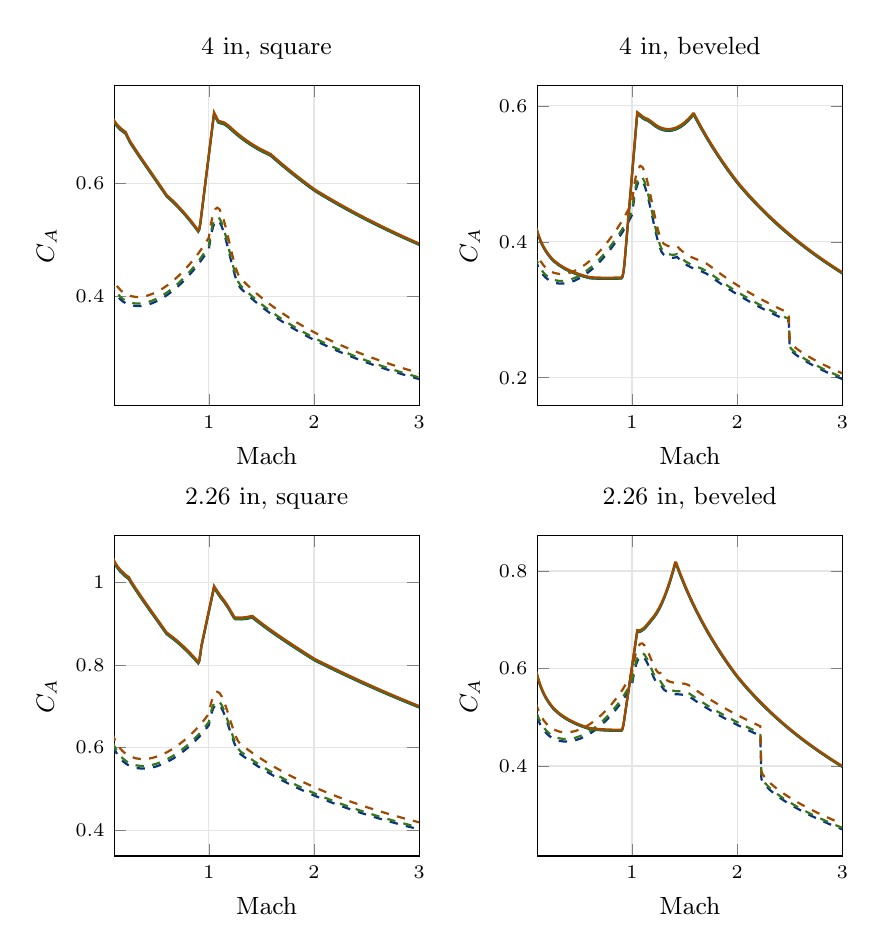
\begin{tikzpicture}
\begin{groupplot}[group style={group size=2 by 2,horizontal sep=1.50cm,vertical sep=1.65cm},width=.45\textwidth,height=5.65cm,grid=major,grid style={gray!20},tick label style={font=\scriptsize},label style={font=\small},title style={font=\small},scaled y ticks=false,yticklabel style={/pgf/number format/fixed,/pgf/number format/precision=3},unbounded coords=jump]
\nextgroupplot[title={4 in, square},xlabel={Mach},ylabel={$C_A$},xmin=0.1,xmax=3]
\addplot[thick,B,dashed] coordinates {(0.01,0.5392703) (0.02,0.4900503) (0.03,0.4658697) (0.04,0.450449) (0.05,0.4393925) (0.06,0.4309168) (0.07,0.424134) (0.08,0.4185425) (0.09,0.4138331) (0.11,0.4063117) (0.13,0.4005716) (0.16,0.3941944) (0.18,0.3910132) (0.21,0.3874247) (0.23,0.3856667) (0.26,0.3838032) (0.31,0.3823806) (0.36,0.3826665) (0.41,0.3843774) (0.46,0.3873356) (0.51,0.3914235) (0.56,0.3965597) (0.61,0.4026861) (0.66,0.40976) (0.71,0.4177495) (0.76,0.4266305) (0.81,0.4363845) (0.86,0.4469972) (0.91,0.4585945) (0.96,0.4716979) (1,0.4829383) (1.01,0.4948939) (1.02,0.5066529) (1.04,0.5223558) (1.06,0.531185) (1.08,0.5340179) (1.1,0.5317335) (1.11,0.5282184) (1.12,0.5247436) (1.14,0.5143528) (1.16,0.5014411) (1.18,0.4868895) (1.21,0.4639718) (1.22,0.4563939) (1.24,0.442215) (1.26,0.4299264) (1.28,0.420412) (1.3,0.4145561) (1.31,0.4127028) (1.36,0.4037825) (1.41,0.3953943) (1.46,0.3874794) (1.51,0.3799903) (1.56,0.3728856) (1.61,0.3661305) (1.66,0.3596946) (1.71,0.3535516) (1.76,0.3476781) (1.81,0.342054) (1.86,0.3366609) (1.91,0.3314828) (1.96,0.3265051) (2.01,0.321715) (2.06,0.3171006) (2.11,0.3126512) (2.16,0.3083573) (2.21,0.3042101) (2.26,0.3002013) (2.31,0.2963238) (2.36,0.2925705) (2.41,0.2889353) (2.46,0.2854124) (2.51,0.2819964) (2.56,0.2786823) (2.61,0.2754654) (2.66,0.2723414) (2.71,0.2693063) (2.76,0.2663562) (2.81,0.2634875) (2.86,0.2606971) (2.91,0.2579816) (2.96,0.2553382) (3,0.2532734)};
\addplot[thick,B] coordinates {(0.01,0.8080247) (0.02,0.7703703) (0.03,0.7516897) (0.04,0.7397161) (0.05,0.7310909) (0.06,0.7244427) (0.07,0.7190856) (0.08,0.7146313) (0.09,0.71084) (0.11,0.7046646) (0.13,0.6997837) (0.16,0.6940281) (0.21,0.6869798) (0.25,0.6717458) (0.26,0.6688288) (0.31,0.6546548) (0.36,0.6409243) (0.41,0.6274162) (0.46,0.6139917) (0.51,0.6005588) (0.56,0.5870533) (0.6,0.5761646) (0.61,0.5745601) (0.66,0.5659074) (0.71,0.5565273) (0.76,0.5463991) (0.81,0.5355068) (0.86,0.5238373) (0.9,0.5139346) (0.91,0.5174294) (0.92,0.5279136) (0.96,0.5879089) (1.01,0.6623833) (1.05,0.7219628) (1.06,0.7181847) (1.09,0.7070495) (1.11,0.7057831) (1.15,0.7035359) (1.16,0.7021903) (1.19,0.6981246) (1.21,0.6946208) (1.26,0.6864266) (1.31,0.6789658) (1.36,0.6721722) (1.41,0.6659967) (1.46,0.660401) (1.51,0.6553543) (1.56,0.6508322) (1.59,0.6480014) (1.61,0.644709) (1.66,0.6366592) (1.71,0.6288397) (1.76,0.6212208) (1.81,0.6137783) (1.86,0.6064927) (1.91,0.5993475) (1.96,0.5923293) (2.01,0.5856607) (2.06,0.5800016) (2.11,0.5744531) (2.16,0.5690102) (2.21,0.5636688) (2.26,0.5584257) (2.31,0.5532778) (2.36,0.5482225) (2.41,0.5432574) (2.46,0.5383803) (2.51,0.533589) (2.56,0.5288813) (2.61,0.5242552) (2.66,0.5197083) (2.71,0.5152385) (2.76,0.5108433) (2.81,0.5065202) (2.86,0.5022668) (2.91,0.4980803) (2.96,0.4939578) (3,0.4907041)};
\addplot[thick,g,dashed] coordinates {(0.01,0.545461) (0.02,0.495676) (0.03,0.4712178) (0.04,0.4556201) (0.05,0.4444366) (0.06,0.4358636) (0.07,0.4290029) (0.08,0.4233473) (0.09,0.4185838) (0.11,0.410976) (0.13,0.4051701) (0.16,0.3987197) (0.18,0.395502) (0.21,0.3918723) (0.23,0.3900941) (0.26,0.3882092) (0.31,0.3867702) (0.36,0.3870595) (0.41,0.38879) (0.46,0.3917821) (0.51,0.3959169) (0.56,0.4011121) (0.61,0.4073088) (0.66,0.4144639) (0.71,0.4225452) (0.76,0.4315281) (0.81,0.4413941) (0.86,0.4521286) (0.91,0.4638591) (0.96,0.4771129) (1,0.4884823) (1.01,0.5005752) (1.02,0.5124692) (1.04,0.5283523) (1.06,0.5372829) (1.08,0.5401483) (1.1,0.5378377) (1.11,0.5342822) (1.12,0.5307675) (1.14,0.5202574) (1.16,0.5071975) (1.18,0.4924789) (1.21,0.4692981) (1.22,0.4616331) (1.24,0.4472915) (1.26,0.4348618) (1.28,0.4252382) (1.3,0.4193151) (1.31,0.4174405) (1.36,0.4084178) (1.41,0.3999333) (1.46,0.3919276) (1.51,0.3843525) (1.56,0.3771662) (1.61,0.3703336) (1.66,0.3638238) (1.71,0.3576103) (1.76,0.3516694) (1.81,0.3459807) (1.86,0.3405257) (1.91,0.3352881) (1.96,0.3302533) (2.01,0.3254082) (2.06,0.3207408) (2.11,0.3162404) (2.16,0.3118972) (2.21,0.3077023) (2.26,0.3036476) (2.31,0.2997255) (2.36,0.2959291) (2.41,0.2922523) (2.46,0.2886889) (2.51,0.2852337) (2.56,0.2818815) (2.61,0.2786277) (2.66,0.2754678) (2.71,0.2723978) (2.76,0.2694139) (2.81,0.2665123) (2.86,0.2636898) (2.91,0.2609432) (2.96,0.2582694) (3,0.2561809)};
\addplot[thick,g] coordinates {(0.01,0.8090101) (0.02,0.7713097) (0.03,0.7526064) (0.04,0.7406181) (0.05,0.7319825) (0.06,0.7253261) (0.07,0.7199625) (0.08,0.7155028) (0.09,0.7117069) (0.11,0.705524) (0.13,0.7006371) (0.16,0.6948744) (0.21,0.6878176) (0.25,0.6725649) (0.26,0.6696444) (0.31,0.6554531) (0.36,0.6417059) (0.41,0.6281813) (0.46,0.6147404) (0.51,0.6012912) (0.56,0.5877692) (0.6,0.5768672) (0.61,0.5752608) (0.66,0.5665975) (0.71,0.5572059) (0.76,0.5470655) (0.81,0.5361598) (0.86,0.5244761) (0.9,0.5145613) (0.91,0.5180604) (0.92,0.5285574) (0.96,0.5886258) (1.01,0.6631911) (1.05,0.7228432) (1.06,0.7190605) (1.09,0.7079117) (1.11,0.7066438) (1.15,0.7043939) (1.16,0.7030465) (1.19,0.6989759) (1.21,0.6954678) (1.26,0.6872636) (1.31,0.6797938) (1.36,0.6729919) (1.41,0.6668089) (1.46,0.6612063) (1.51,0.6561534) (1.56,0.6516258) (1.59,0.6487916) (1.61,0.6454952) (1.66,0.6374356) (1.71,0.6296065) (1.76,0.6219783) (1.81,0.6145268) (1.86,0.6072323) (1.91,0.6000784) (1.96,0.5930516) (2.01,0.5863749) (2.06,0.5807089) (2.11,0.5751536) (2.16,0.5697041) (2.21,0.5643562) (2.26,0.5591067) (2.31,0.5539525) (2.36,0.5488911) (2.41,0.5439198) (2.46,0.5390368) (2.51,0.5342397) (2.56,0.5295263) (2.61,0.5248945) (2.66,0.520342) (2.71,0.5158668) (2.76,0.5114662) (2.81,0.5071379) (2.86,0.5028793) (2.91,0.4986877) (2.96,0.4945602) (3,0.4913025)};
\addplot[thick,burntorange,dashed] coordinates {(0.01,0.5619255) (0.02,0.5106378) (0.03,0.4854414) (0.04,0.4693728) (0.05,0.4578518) (0.06,0.44902) (0.07,0.4419523) (0.08,0.4361259) (0.09,0.4312187) (0.11,0.4233812) (0.13,0.4174) (0.16,0.4107549) (0.18,0.4074401) (0.21,0.4037008) (0.23,0.4018689) (0.26,0.3999271) (0.31,0.3984448) (0.36,0.3987427) (0.41,0.4005255) (0.46,0.403608) (0.51,0.4078676) (0.56,0.4132196) (0.61,0.4196033) (0.66,0.4269744) (0.71,0.4352996) (0.76,0.4445537) (0.81,0.4547174) (0.86,0.465776) (0.91,0.4778606) (0.96,0.4915144) (1,0.503227) (1.01,0.5156849) (1.02,0.5279379) (1.04,0.5443005) (1.06,0.5535006) (1.08,0.5564525) (1.1,0.5540722) (1.11,0.5504094) (1.12,0.5467886) (1.14,0.5359612) (1.16,0.5225071) (1.18,0.5073442) (1.21,0.4834637) (1.22,0.4755674) (1.24,0.4607928) (1.26,0.447988) (1.28,0.4380739) (1.3,0.431972) (1.31,0.4300409) (1.36,0.4207458) (1.41,0.4120052) (1.46,0.4037578) (1.51,0.3959541) (1.56,0.3885509) (1.61,0.381512) (1.66,0.3748057) (1.71,0.3684046) (1.76,0.3622844) (1.81,0.356424) (1.86,0.3508044) (1.91,0.3454087) (1.96,0.3402219) (2.01,0.3352306) (2.06,0.3304223) (2.11,0.325786) (2.16,0.3213117) (2.21,0.3169902) (2.26,0.3128131) (2.31,0.3087726) (2.36,0.3048617) (2.41,0.3010738) (2.46,0.2974029) (2.51,0.2938434) (2.56,0.29039) (2.61,0.287038) (2.66,0.2837827) (2.71,0.2806201) (2.76,0.277546) (2.81,0.2745569) (2.86,0.2716492) (2.91,0.2688197) (2.96,0.2660652) (3,0.2639137)};
\addplot[thick,burntorange] coordinates {(0.01,0.8119758) (0.02,0.7741372) (0.03,0.7553653) (0.04,0.7433331) (0.05,0.7346658) (0.06,0.727985) (0.07,0.7226017) (0.08,0.7181257) (0.09,0.7143159) (0.11,0.7081103) (0.13,0.7032055) (0.16,0.6974217) (0.21,0.690339) (0.25,0.6750304) (0.26,0.6720992) (0.31,0.6578559) (0.36,0.6440583) (0.41,0.6304841) (0.46,0.6169939) (0.51,0.6034954) (0.56,0.5899238) (0.6,0.5789819) (0.61,0.5773696) (0.66,0.5686746) (0.71,0.5592485) (0.76,0.5490709) (0.81,0.5381253) (0.86,0.5263988) (0.9,0.5164476) (0.91,0.5199595) (0.92,0.530495) (0.96,0.5907836) (1.01,0.6656222) (1.05,0.725493) (1.06,0.7216965) (1.09,0.7105068) (1.11,0.7092342) (1.15,0.706976) (1.16,0.7056238) (1.19,0.7015382) (1.21,0.6980173) (1.26,0.689783) (1.31,0.6822858) (1.36,0.675459) (1.41,0.6692533) (1.46,0.6636302) (1.51,0.6585588) (1.56,0.6540146) (1.59,0.65117) (1.61,0.6478615) (1.66,0.6397723) (1.71,0.6319145) (1.76,0.6242584) (1.81,0.6167795) (1.86,0.6094583) (1.91,0.6022782) (1.96,0.5952256) (2.01,0.5885244) (2.06,0.5828377) (2.11,0.577262) (2.16,0.5717926) (2.21,0.566425) (2.26,0.5611563) (2.31,0.5559831) (2.36,0.5509032) (2.41,0.5459138) (2.46,0.5410128) (2.51,0.5361981) (2.56,0.5314674) (2.61,0.5268186) (2.66,0.5222495) (2.71,0.5177579) (2.76,0.5133412) (2.81,0.508997) (2.86,0.5047228) (2.91,0.5005158) (2.96,0.4963732) (3,0.4931035)};
\nextgroupplot[title={4 in, beveled},xlabel={Mach},ylabel={$C_A$},xmin=0.1,xmax=3]
\addplot[thick,B,dashed] coordinates {(0.01,0.4955621) (0.02,0.4463415) (0.03,0.4221597) (0.04,0.4067373) (0.05,0.3956786) (0.06,0.3872002) (0.07,0.3804143) (0.08,0.3748193) (0.09,0.3701059) (0.11,0.3625749) (0.13,0.3568235) (0.16,0.3504259) (0.18,0.3472289) (0.21,0.3436136) (0.23,0.3418356) (0.26,0.3399392) (0.31,0.3384548) (0.36,0.3386713) (0.41,0.3403069) (0.46,0.3431862) (0.51,0.3471947) (0.56,0.3522544) (0.61,0.3583117) (0.66,0.3653296) (0.71,0.3732834) (0.76,0.3821579) (0.81,0.3919458) (0.86,0.4026476) (0.91,0.4144078) (0.96,0.4277726) (1,0.4393144) (1.01,0.4510799) (1.02,0.4629209) (1.04,0.4788217) (1.06,0.4878998) (1.08,0.4910396) (1.1,0.4891272) (1.11,0.4858248) (1.12,0.4825817) (1.14,0.4727157) (1.16,0.4604176) (1.18,0.4465782) (1.21,0.4249381) (1.22,0.4178484) (1.24,0.404751) (1.26,0.3936996) (1.28,0.3856) (1.3,0.3813638) (1.31,0.3804075) (1.34,0.37809) (1.36,0.3770685) (1.39,0.3764987) (1.41,0.376916) (1.43,0.3775066) (1.46,0.3727592) (1.51,0.366726) (1.56,0.3625256) (1.61,0.3594235) (1.66,0.3565539) (1.71,0.3529445) (1.76,0.3476781) (1.81,0.342054) (1.86,0.3366609) (1.91,0.3314828) (1.96,0.3265051) (2.01,0.321715) (2.06,0.3171006) (2.11,0.3126512) (2.16,0.3083573) (2.21,0.3042101) (2.26,0.3002013) (2.31,0.2963238) (2.36,0.2925705) (2.41,0.2889353) (2.46,0.2854124) (2.49,0.2833503) (2.5,0.2430483) (2.51,0.240604) (2.53,0.2374095) (2.56,0.233615) (2.61,0.2282684) (2.66,0.2235344) (2.71,0.2191793) (2.76,0.2151014) (2.81,0.2112445) (2.86,0.2075729) (2.91,0.2040619) (2.96,0.2006932) (3,0.1980912)};
\addplot[thick,B] coordinates {(0.01,0.5863164) (0.02,0.5211986) (0.03,0.4891801) (0.04,0.4687447) (0.05,0.4540613) (0.06,0.442762) (0.07,0.4336675) (0.08,0.4261116) (0.09,0.4196841) (0.1,0.4141154) (0.11,0.4092202) (0.13,0.4009531) (0.14,0.3974088) (0.16,0.3912058) (0.18,0.3859236) (0.21,0.3792669) (0.24,0.3737261) (0.26,0.3706882) (0.31,0.3647434) (0.36,0.3600281) (0.41,0.3561808) (0.46,0.3529754) (0.51,0.3502616) (0.56,0.3479347) (0.6,0.3463006) (0.61,0.3462077) (0.66,0.3458135) (0.71,0.3455966) (0.76,0.3455285) (0.81,0.3455865) (0.86,0.3457523) (0.9,0.3459527) (0.91,0.3483052) (0.92,0.3553626) (0.93,0.3697444) (0.96,0.4242766) (1.01,0.5151636) (1.05,0.5878732) (1.06,0.5866429) (1.11,0.5807182) (1.13,0.5790303) (1.15,0.5780496) (1.16,0.576851) (1.19,0.5736579) (1.21,0.5710699) (1.23,0.5688669) (1.26,0.5662524) (1.28,0.564955) (1.31,0.5636602) (1.33,0.5632242) (1.36,0.5632031) (1.38,0.5636076) (1.41,0.5648392) (1.43,0.5660756) (1.46,0.5685528) (1.49,0.5717779) (1.51,0.5743443) (1.54,0.5788208) (1.56,0.5822248) (1.58,0.5859661) (1.59,0.5858598) (1.61,0.5799547) (1.66,0.5658094) (1.71,0.5524506) (1.76,0.5397811) (1.81,0.5277226) (1.86,0.5162118) (1.91,0.5051956) (1.96,0.4946296) (2.01,0.4846276) (2.06,0.475588) (2.11,0.4669043) (2.16,0.4585525) (2.21,0.4505112) (2.26,0.4427617) (2.31,0.4352867) (2.36,0.4280706) (2.41,0.4210989) (2.46,0.4143585) (2.51,0.4078372) (2.56,0.4015231) (2.61,0.3954055) (2.66,0.3894743) (2.71,0.3837197) (2.76,0.3781323) (2.81,0.3727032) (2.86,0.3674241) (2.91,0.3622866) (2.96,0.3572828) (3,0.3533708)};
\addplot[thick,g,dashed] coordinates {(0.01,0.501251) (0.02,0.4514653) (0.03,0.4270059) (0.04,0.4114065) (0.05,0.4002209) (0.06,0.3916452) (0.07,0.3847814) (0.08,0.3791221) (0.09,0.3743546) (0.11,0.3667372) (0.13,0.3609197) (0.16,0.3544487) (0.18,0.351215) (0.21,0.3475582) (0.23,0.3457598) (0.26,0.3438416) (0.31,0.3423401) (0.36,0.3425591) (0.41,0.3442135) (0.46,0.3471259) (0.51,0.3511804) (0.56,0.3562982) (0.61,0.362425) (0.66,0.3695235) (0.71,0.3775686) (0.76,0.3865449) (0.81,0.3964452) (0.86,0.4072699) (0.91,0.4191651) (0.96,0.4326833) (1,0.4443577) (1.01,0.4562582) (1.02,0.4682351) (1.04,0.4843185) (1.06,0.4935008) (1.08,0.4966766) (1.1,0.4947423) (1.11,0.491402) (1.12,0.4881217) (1.14,0.4781423) (1.16,0.4657031) (1.18,0.4517048) (1.21,0.4298163) (1.22,0.4226452) (1.24,0.4093975) (1.26,0.3982192) (1.28,0.3900266) (1.3,0.3857417) (1.31,0.3847745) (1.34,0.3824304) (1.36,0.3813971) (1.39,0.3808208) (1.41,0.3812429) (1.43,0.3818403) (1.46,0.3770384) (1.51,0.370936) (1.56,0.3666873) (1.61,0.3635496) (1.66,0.3606471) (1.71,0.3569962) (1.76,0.3516694) (1.81,0.3459807) (1.86,0.3405257) (1.91,0.3352881) (1.96,0.3302533) (2.01,0.3254082) (2.06,0.3207408) (2.11,0.3162404) (2.16,0.3118972) (2.21,0.3077023) (2.26,0.3036476) (2.31,0.2997255) (2.36,0.2959291) (2.41,0.2922523) (2.46,0.2886889) (2.49,0.2866031) (2.5,0.2458384) (2.51,0.2433661) (2.53,0.2401349) (2.56,0.2362969) (2.61,0.2308889) (2.66,0.2261005) (2.71,0.2216954) (2.76,0.2175707) (2.81,0.2136696) (2.86,0.2099558) (2.91,0.2064044) (2.96,0.2029971) (3,0.2003652)};
\addplot[thick,g] coordinates {(0.01,0.5870314) (0.02,0.5218341) (0.03,0.4897767) (0.04,0.4693163) (0.05,0.454615) (0.06,0.4433019) (0.07,0.4341963) (0.08,0.4266312) (0.09,0.4201959) (0.1,0.4146204) (0.11,0.4097192) (0.13,0.4014421) (0.14,0.3978934) (0.16,0.3916829) (0.18,0.3863942) (0.21,0.3797294) (0.24,0.3741818) (0.26,0.3711403) (0.31,0.3651882) (0.36,0.3604671) (0.41,0.3566151) (0.46,0.3534058) (0.51,0.3506887) (0.56,0.348359) (0.6,0.3467229) (0.61,0.3466299) (0.66,0.3462352) (0.71,0.3460181) (0.76,0.3459499) (0.81,0.3460079) (0.86,0.3461739) (0.9,0.3463746) (0.91,0.3487299) (0.92,0.355796) (0.93,0.3701953) (0.96,0.424794) (1.01,0.5157918) (1.05,0.5885901) (1.06,0.5873583) (1.11,0.5814263) (1.13,0.5797364) (1.15,0.5787545) (1.16,0.5775545) (1.19,0.5743575) (1.21,0.5717663) (1.23,0.5695606) (1.26,0.5669429) (1.28,0.565644) (1.31,0.5643476) (1.33,0.563911) (1.36,0.5638899) (1.38,0.5642949) (1.41,0.565528) (1.43,0.5667659) (1.46,0.5692462) (1.49,0.5724752) (1.51,0.5750447) (1.54,0.5795267) (1.56,0.5829348) (1.58,0.5866806) (1.59,0.5865743) (1.61,0.5806619) (1.66,0.5664994) (1.71,0.5531243) (1.76,0.5404393) (1.81,0.5283661) (1.86,0.5168413) (1.91,0.5058117) (1.96,0.4952328) (2.01,0.4852185) (2.06,0.476168) (2.11,0.4674736) (2.16,0.4591117) (2.21,0.4510606) (2.26,0.4433016) (2.31,0.4358175) (2.36,0.4285926) (2.41,0.4216124) (2.46,0.4148638) (2.51,0.4083345) (2.56,0.4020127) (2.61,0.3958877) (2.66,0.3899492) (2.71,0.3841876) (2.76,0.3785934) (2.81,0.3731577) (2.86,0.3678722) (2.91,0.3627284) (2.96,0.3577185) (3,0.3538018)};
\addplot[thick,burntorange,dashed] coordinates {(0.01,0.5163812) (0.02,0.4650927) (0.03,0.439895) (0.04,0.4238247) (0.05,0.4123014) (0.06,0.4034669) (0.07,0.3963959) (0.08,0.3905658) (0.09,0.3856544) (0.11,0.377807) (0.13,0.371814) (0.16,0.3651477) (0.18,0.3618164) (0.21,0.3580491) (0.23,0.3561964) (0.26,0.3542204) (0.31,0.3526736) (0.36,0.3528992) (0.41,0.3546035) (0.46,0.3576038) (0.51,0.3617807) (0.56,0.3670529) (0.61,0.3733647) (0.66,0.3806775) (0.71,0.3889654) (0.76,0.3982127) (0.81,0.4084118) (0.86,0.4195632) (0.91,0.4318175) (0.96,0.4457437) (1,0.4577705) (1.01,0.4700302) (1.02,0.4823687) (1.04,0.4989375) (1.06,0.508397) (1.08,0.5116687) (1.1,0.5096759) (1.11,0.5062348) (1.12,0.5028555) (1.14,0.4925749) (1.16,0.4797602) (1.18,0.4653394) (1.21,0.4427901) (1.22,0.4354026) (1.24,0.421755) (1.26,0.4102393) (1.28,0.4017995) (1.3,0.3973852) (1.31,0.3963888) (1.34,0.3939739) (1.36,0.3929095) (1.39,0.3923158) (1.41,0.3927506) (1.43,0.393366) (1.46,0.3884192) (1.51,0.3821326) (1.56,0.3777557) (1.61,0.3745233) (1.66,0.3715331) (1.71,0.3677721) (1.76,0.3622844) (1.81,0.356424) (1.86,0.3508044) (1.91,0.3454087) (1.96,0.3402219) (2.01,0.3352306) (2.06,0.3304223) (2.11,0.325786) (2.16,0.3213117) (2.21,0.3169902) (2.26,0.3128131) (2.31,0.3087726) (2.36,0.3048617) (2.41,0.3010738) (2.46,0.2974029) (2.49,0.2952542) (2.5,0.253259) (2.51,0.250712) (2.53,0.2473833) (2.56,0.2434294) (2.61,0.2378582) (2.66,0.2329253) (2.71,0.2283872) (2.76,0.2241381) (2.81,0.2201191) (2.86,0.2162933) (2.91,0.2126347) (2.96,0.2091245) (3,0.2064132)};
\addplot[thick,burntorange] coordinates {(0.01,0.5891833) (0.02,0.5237471) (0.03,0.4915721) (0.04,0.4710367) (0.05,0.4562816) (0.06,0.444927) (0.07,0.435788) (0.08,0.4281952) (0.09,0.4217362) (0.1,0.4161404) (0.11,0.4112212) (0.13,0.4029137) (0.14,0.399352) (0.16,0.3931187) (0.18,0.3878106) (0.21,0.3811214) (0.24,0.3755535) (0.26,0.3725008) (0.31,0.3665269) (0.36,0.3617885) (0.41,0.3579224) (0.46,0.3547013) (0.51,0.3519743) (0.56,0.3496361) (0.6,0.3479939) (0.61,0.3479006) (0.66,0.3475044) (0.71,0.3472865) (0.76,0.3472181) (0.81,0.3472763) (0.86,0.347443) (0.9,0.3476443) (0.91,0.3500083) (0.92,0.3571002) (0.93,0.3715523) (0.96,0.4263512) (1.01,0.5176826) (1.05,0.5907478) (1.06,0.5895114) (1.11,0.5835577) (1.13,0.5818616) (1.15,0.5808761) (1.16,0.5796717) (1.19,0.576463) (1.21,0.5738623) (1.23,0.5716485) (1.26,0.5690213) (1.28,0.5677175) (1.31,0.5664164) (1.33,0.5659782) (1.36,0.565957) (1.38,0.5663635) (1.41,0.5676011) (1.43,0.5688435) (1.46,0.5713329) (1.49,0.5745738) (1.51,0.5771527) (1.54,0.5816511) (1.56,0.5850717) (1.58,0.5888313) (1.59,0.5887246) (1.61,0.5827905) (1.66,0.5685761) (1.71,0.555152) (1.76,0.5424205) (1.81,0.530303) (1.86,0.5187359) (1.91,0.5076659) (1.96,0.4970483) (2.01,0.4869973) (2.06,0.4779135) (2.11,0.4691873) (2.16,0.4607947) (2.21,0.4527141) (2.26,0.4449267) (2.31,0.4374151) (2.36,0.4301638) (2.41,0.423158) (2.46,0.4163846) (2.51,0.4098314) (2.56,0.4034864) (2.61,0.397339) (2.66,0.3913787) (2.71,0.385596) (2.76,0.3799813) (2.81,0.3745257) (2.86,0.3692207) (2.91,0.3640581) (2.96,0.3590298) (3,0.3550987)};
\nextgroupplot[title={2.26 in, square},xlabel={Mach},ylabel={$C_A$},xmin=0.1,xmax=3]
\addplot[thick,B,dashed] coordinates {(0.01,0.8020017) (0.02,0.7245741) (0.03,0.686642) (0.04,0.6624746) (0.05,0.6451456) (0.06,0.6318502) (0.07,0.6211938) (0.08,0.6123893) (0.09,0.604952) (0.1,0.5985638) (0.11,0.5930054) (0.13,0.5837918) (0.16,0.5733641) (0.18,0.5680205) (0.21,0.5617585) (0.23,0.5585117) (0.26,0.5547559) (0.31,0.5508767) (0.36,0.549358) (0.41,0.5497589) (0.46,0.5518042) (0.51,0.5553118) (0.56,0.5601566) (0.61,0.5662493) (0.66,0.5735252) (0.71,0.5819362) (0.76,0.5914465) (0.81,0.602029) (0.86,0.6136636) (0.91,0.6265437) (0.96,0.6414652) (1,0.654376) (1.01,0.6666112) (1.02,0.6783271) (1.04,0.6939761) (1.06,0.7027898) (1.08,0.7056421) (1.1,0.7034092) (1.11,0.6998117) (1.12,0.696256) (1.14,0.6857068) (1.16,0.6726397) (1.18,0.6579336) (1.21,0.634783) (1.24,0.6127886) (1.26,0.6003375) (1.28,0.5906565) (1.3,0.5846293) (1.31,0.5826885) (1.36,0.573312) (1.41,0.5644364) (1.46,0.5560049) (1.51,0.547972) (1.56,0.5402991) (1.61,0.5329543) (1.66,0.5259098) (1.71,0.5191422) (1.76,0.5126306) (1.81,0.5063573) (1.86,0.5003061) (1.91,0.494463) (1.96,0.4888153) (2.01,0.4833517) (2.06,0.478062) (2.11,0.4729368) (2.16,0.4679677) (2.21,0.463147) (2.26,0.4584675) (2.31,0.4539226) (2.36,0.4495064) (2.41,0.4452132) (2.46,0.4410376) (2.51,0.436975) (2.56,0.4330207) (2.61,0.4291704) (2.66,0.4254201) (2.71,0.4217661) (2.76,0.4182047) (2.81,0.4147327) (2.86,0.4113467) (2.91,0.4080438) (2.96,0.4048212) (3,0.4022989)};
\addplot[thick,B] coordinates {(0.01,1.21345) (0.02,1.15217) (0.03,1.121582) (0.04,1.101885) (0.05,1.087644) (0.06,1.076632) (0.07,1.067733) (0.08,1.060314) (0.09,1.053986) (0.11,1.043646) (0.13,1.035442) (0.16,1.02573) (0.21,1.01377) (0.24,1.008194) (0.26,0.9992) (0.31,0.9796375) (0.36,0.9609273) (0.41,0.9427009) (0.46,0.9247262) (0.51,0.9068487) (0.56,0.8889601) (0.6,0.8745881) (0.61,0.8728513) (0.66,0.8632907) (0.71,0.8528037) (0.76,0.8413554) (0.81,0.828918) (0.86,0.8154694) (0.9,0.8039702) (0.91,0.8094372) (0.92,0.8258382) (0.93,0.8440995) (0.96,0.8798626) (1.01,0.9394678) (1.05,0.987152) (1.06,0.9829413) (1.11,0.9638933) (1.15,0.9508898) (1.16,0.9469838) (1.19,0.9354468) (1.21,0.9264695) (1.24,0.9136873) (1.25,0.911202) (1.26,0.9109504) (1.31,0.9106605) (1.36,0.9119237) (1.41,0.9146808) (1.42,0.9137596) (1.46,0.905556) (1.51,0.8957788) (1.56,0.8864102) (1.61,0.8773532) (1.66,0.8685357) (1.71,0.8599042) (1.76,0.8514182) (1.81,0.8430476) (1.86,0.8347701) (1.91,0.8265688) (1.96,0.8184316) (2.01,0.8106998) (2.06,0.8043691) (2.11,0.7981008) (2.16,0.7918947) (2.21,0.785751) (2.26,0.7796708) (2.31,0.7736552) (2.36,0.7677052) (2.41,0.7618215) (2.46,0.7560053) (2.51,0.7502567) (2.56,0.7445758) (2.61,0.7389624) (2.66,0.7334156) (2.71,0.7279346) (2.76,0.7225177) (2.81,0.7171629) (2.86,0.7118681) (2.91,0.7066306) (2.96,0.7014473) (3,0.6973375)};
\addplot[thick,g,dashed] coordinates {(0.01,0.8112084) (0.02,0.732892) (0.03,0.6945245) (0.04,0.6700797) (0.05,0.6525517) (0.06,0.6391037) (0.07,0.628325) (0.08,0.6194194) (0.09,0.6118967) (0.1,0.6054351) (0.11,0.599813) (0.13,0.5904936) (0.16,0.5799462) (0.18,0.5745412) (0.21,0.5682074) (0.23,0.5649233) (0.26,0.5611243) (0.31,0.5572006) (0.36,0.5556645) (0.41,0.55607) (0.46,0.5581387) (0.51,0.5616866) (0.56,0.566587) (0.61,0.5727497) (0.66,0.5801091) (0.71,0.5886167) (0.76,0.5982361) (0.81,0.6089402) (0.86,0.6207084) (0.91,0.6337362) (0.96,0.6488291) (1,0.661888) (1.01,0.6742637) (1.02,0.6861142) (1.04,0.7019427) (1.06,0.7108576) (1.08,0.7137427) (1.1,0.7114842) (1.11,0.7078454) (1.12,0.7042488) (1.14,0.6935786) (1.16,0.6803614) (1.18,0.6654865) (1.21,0.6420701) (1.24,0.6198232) (1.26,0.6072292) (1.28,0.597437) (1.3,0.5913407) (1.31,0.5893776) (1.36,0.5798935) (1.41,0.570916) (1.46,0.5623877) (1.51,0.5542626) (1.56,0.5465016) (1.61,0.5390725) (1.66,0.5319471) (1.71,0.5251018) (1.76,0.5185155) (1.81,0.5121701) (1.86,0.5060495) (1.91,0.5001393) (1.96,0.4944268) (2.01,0.4889005) (2.06,0.48355) (2.11,0.478366) (2.16,0.4733399) (2.21,0.4684638) (2.26,0.4637306) (2.31,0.4591336) (2.36,0.4546666) (2.41,0.4503241) (2.46,0.4461006) (2.51,0.4419914) (2.56,0.4379917) (2.61,0.4340972) (2.66,0.4303039) (2.71,0.4266079) (2.76,0.4230056) (2.81,0.4194937) (2.86,0.4160689) (2.91,0.4127281) (2.96,0.4094684) (3,0.4069172)};
\addplot[thick,g] coordinates {(0.01,1.21493) (0.02,1.153575) (0.03,1.122949) (0.04,1.103229) (0.05,1.08897) (0.06,1.077944) (0.07,1.069035) (0.08,1.061608) (0.09,1.055271) (0.11,1.044918) (0.13,1.036705) (0.16,1.02698) (0.21,1.015006) (0.24,1.009423) (0.26,1.000419) (0.31,0.9808322) (0.36,0.9620991) (0.41,0.9438504) (0.46,0.9258539) (0.51,0.9079546) (0.56,0.8900442) (0.6,0.8756546) (0.61,0.8739157) (0.66,0.8643434) (0.71,0.8538437) (0.76,0.8423814) (0.81,0.8299289) (0.86,0.8164639) (0.9,0.8049506) (0.91,0.8104243) (0.92,0.8268453) (0.93,0.8451288) (0.96,0.8809355) (1.01,0.9406134) (1.05,0.9883557) (1.06,0.9841399) (1.11,0.9650687) (1.15,0.9520494) (1.16,0.9481386) (1.19,0.9365875) (1.21,0.9275993) (1.24,0.9148016) (1.25,0.9123132) (1.26,0.9120613) (1.31,0.911771) (1.36,0.9130357) (1.41,0.9157962) (1.42,0.9148739) (1.46,0.9066603) (1.51,0.8968712) (1.56,0.8874912) (1.61,0.8784231) (1.66,0.8695949) (1.71,0.8609528) (1.76,0.8524564) (1.81,0.8440757) (1.86,0.835788) (1.91,0.8275768) (1.96,0.8194297) (2.01,0.8116884) (2.06,0.80535) (2.11,0.799074) (2.16,0.7928604) (2.21,0.7867092) (2.26,0.7806216) (2.31,0.7745986) (2.36,0.7686413) (2.41,0.7627506) (2.46,0.7569272) (2.51,0.7511716) (2.56,0.7454838) (2.61,0.7398635) (2.66,0.73431) (2.71,0.7288223) (2.76,0.7233988) (2.81,0.7180375) (2.86,0.7127362) (2.91,0.7074923) (2.96,0.7023027) (3,0.6981879)};
\addplot[thick,burntorange,dashed] coordinates {(0.01,0.8356946) (0.02,0.7550142) (0.03,0.7154885) (0.04,0.6903058) (0.05,0.6722488) (0.06,0.6583948) (0.07,0.6472908) (0.08,0.6381164) (0.09,0.6303666) (0.1,0.62371) (0.11,0.6179182) (0.13,0.6083175) (0.16,0.5974517) (0.18,0.5918836) (0.21,0.5853585) (0.23,0.5819753) (0.26,0.5780617) (0.31,0.5740196) (0.36,0.5724371) (0.41,0.5728549) (0.46,0.574986) (0.51,0.578641) (0.56,0.5836893) (0.61,0.590038) (0.66,0.5976195) (0.71,0.6063839) (0.76,0.6162937) (0.81,0.6273209) (0.86,0.6394443) (0.91,0.6528654) (0.96,0.6684138) (1,0.681867) (1.01,0.6946162) (1.02,0.7068243) (1.04,0.7231307) (1.06,0.7323147) (1.08,0.7352869) (1.1,0.7329601) (1.11,0.7292115) (1.12,0.7255064) (1.14,0.714514) (1.16,0.7008979) (1.18,0.6855741) (1.21,0.6614509) (1.24,0.6385324) (1.26,0.6255582) (1.28,0.6154705) (1.3,0.6091902) (1.31,0.6071678) (1.36,0.5973974) (1.41,0.5881489) (1.46,0.5793632) (1.51,0.5709928) (1.56,0.5629976) (1.61,0.5553442) (1.66,0.5480038) (1.71,0.5409519) (1.76,0.5341668) (1.81,0.5276299) (1.86,0.5213244) (1.91,0.5152359) (1.96,0.5093509) (2.01,0.5036578) (2.06,0.4981458) (2.11,0.4928054) (2.16,0.4876275) (2.21,0.4826043) (2.26,0.4777282) (2.31,0.4729924) (2.36,0.4683906) (2.41,0.463917) (2.46,0.4595661) (2.51,0.4553328) (2.56,0.4512123) (2.61,0.4472003) (2.66,0.4432925) (2.71,0.4394849) (2.76,0.4357739) (2.81,0.432156) (2.86,0.4286278) (2.91,0.4251862) (2.96,0.4218281) (3,0.4191999)};
\addplot[thick,burntorange] coordinates {(0.01,1.219384) (0.02,1.157804) (0.03,1.127066) (0.04,1.107273) (0.05,1.092962) (0.06,1.081896) (0.07,1.072954) (0.08,1.065499) (0.09,1.05914) (0.11,1.048749) (0.13,1.040505) (0.16,1.030745) (0.21,1.018727) (0.24,1.013124) (0.26,1.004086) (0.31,0.9844277) (0.36,0.965626) (0.41,0.9473104) (0.46,0.9292479) (0.51,0.911283) (0.56,0.8933069) (0.6,0.8788646) (0.61,0.8771193) (0.66,0.867512) (0.71,0.8569737) (0.76,0.8454695) (0.81,0.8329712) (0.86,0.8194569) (0.9,0.8079014) (0.91,0.8133951) (0.92,0.8298763) (0.93,0.8482269) (0.96,0.8841649) (1.01,0.9440616) (1.05,0.9919789) (1.06,0.9877476) (1.11,0.9686065) (1.15,0.9555395) (1.16,0.9516143) (1.19,0.9400209) (1.21,0.9309998) (1.24,0.9181551) (1.25,0.9156576) (1.26,0.9154047) (1.31,0.9151134) (1.36,0.9163827) (1.41,0.9191534) (1.42,0.9182276) (1.46,0.9099839) (1.51,0.900159) (1.56,0.8907446) (1.61,0.8816432) (1.66,0.8727827) (1.71,0.8641089) (1.76,0.8555814) (1.81,0.8471699) (1.86,0.8388519) (1.91,0.8306105) (1.96,0.8224336) (2.01,0.8146639) (2.06,0.8083022) (2.11,0.8020033) (2.16,0.7957669) (2.21,0.7895931) (2.26,0.7834832) (2.31,0.7774381) (2.36,0.7714591) (2.41,0.7655467) (2.46,0.7597019) (2.51,0.7539253) (2.56,0.7482166) (2.61,0.7425757) (2.66,0.7370019) (2.71,0.731494) (2.76,0.7260506) (2.81,0.7206697) (2.86,0.715349) (2.91,0.7100858) (2.96,0.7048772) (3,0.7007473)};
\nextgroupplot[title={2.26 in, beveled},xlabel={Mach},ylabel={$C_A$},xmin=0.1,xmax=3]
\addplot[thick,B,dashed] coordinates {(0.01,0.7026778) (0.02,0.6252501) (0.03,0.5873178) (0.04,0.5631501) (0.05,0.5458206) (0.06,0.5325248) (0.07,0.5218679) (0.08,0.5130628) (0.09,0.5056248) (0.11,0.4936768) (0.13,0.4844618) (0.16,0.4740324) (0.18,0.4686881) (0.21,0.4624263) (0.23,0.4591809) (0.26,0.4554296) (0.31,0.451568) (0.36,0.4500849) (0.41,0.4505481) (0.46,0.4526929) (0.51,0.4563512) (0.56,0.4614147) (0.61,0.467816) (0.66,0.4755179) (0.71,0.4845079) (0.76,0.4947961) (0.81,0.5064156) (0.86,0.5194266) (0.91,0.5341312) (0.96,0.5514768) (1,0.5669007) (1.01,0.579224) (1.02,0.5916759) (1.04,0.6089701) (1.06,0.6196922) (1.08,0.624758) (1.1,0.6250922) (1.11,0.6229284) (1.12,0.6209173) (1.14,0.6138277) (1.16,0.6047883) (1.21,0.5802996) (1.22,0.576058) (1.24,0.5695491) (1.26,0.5665903) (1.27,0.567274) (1.3,0.5576188) (1.31,0.5558206) (1.33,0.5528389) (1.36,0.5497526) (1.41,0.5474347) (1.46,0.546845) (1.51,0.5454447) (1.54,0.5429981) (1.56,0.5402991) (1.61,0.5329543) (1.66,0.5259098) (1.71,0.5191422) (1.76,0.5126306) (1.81,0.5063573) (1.86,0.5003061) (1.91,0.494463) (1.96,0.4888153) (2.01,0.4833517) (2.06,0.478062) (2.11,0.4729368) (2.16,0.4679677) (2.21,0.463147) (2.22,0.4622) (2.23,0.3736896) (2.24,0.3685991) (2.26,0.3622825) (2.28,0.3573525) (2.31,0.3510586) (2.36,0.3420837) (2.41,0.3341971) (2.46,0.3270167) (2.51,0.3203572) (2.56,0.3141106) (2.61,0.3082067) (2.66,0.3025961) (2.71,0.2972425) (2.76,0.2921178) (2.81,0.2871996) (2.86,0.2824696) (2.91,0.2779126) (2.96,0.2735157) (3,0.2701059)};
\addplot[thick,B] coordinates {(0.01,0.8502291) (0.02,0.7500316) (0.03,0.7005872) (0.04,0.6689448) (0.05,0.6461587) (0.06,0.6285909) (0.07,0.6144273) (0.08,0.6026425) (0.09,0.5926037) (0.1,0.5838954) (0.11,0.5762313) (0.13,0.5632676) (0.14,0.5577012) (0.16,0.5479464) (0.18,0.5396255) (0.21,0.5291198) (0.24,0.5203569) (0.26,0.5155081) (0.31,0.5058939) (0.36,0.4982169) (0.41,0.4919111) (0.46,0.4866213) (0.51,0.4821112) (0.56,0.4782162) (0.61,0.4752168) (0.66,0.4741182) (0.71,0.47331) (0.76,0.4727461) (0.81,0.4723897) (0.86,0.4722117) (0.9,0.4721813) (0.91,0.4753922) (0.92,0.4850247) (0.96,0.5435473) (1.01,0.6168306) (1.05,0.6754572) (1.06,0.6749282) (1.08,0.6755975) (1.11,0.6795852) (1.13,0.6838852) (1.16,0.6916455) (1.21,0.7048008) (1.23,0.7109227) (1.26,0.7221127) (1.28,0.7308994) (1.31,0.7460596) (1.34,0.7635931) (1.36,0.7766027) (1.39,0.798106) (1.41,0.8137736) (1.42,0.8137167) (1.46,0.7906987) (1.51,0.7643288) (1.56,0.7401393) (1.61,0.7177466) (1.66,0.6968658) (1.71,0.6772797) (1.76,0.6588187) (1.81,0.6413474) (1.86,0.6247559) (1.91,0.6089533) (1.96,0.5938635) (2.01,0.5796419) (2.06,0.5668599) (2.11,0.554629) (2.16,0.5429089) (2.21,0.5316634) (2.26,0.5208607) (2.31,0.5104719) (2.36,0.500471) (2.41,0.4908337) (2.46,0.4815383) (2.51,0.4725643) (2.56,0.4638924) (2.61,0.455505) (2.66,0.447385) (2.71,0.4395167) (2.76,0.4318847) (2.81,0.4244746) (2.86,0.4172726) (2.91,0.4102652) (2.96,0.4034396) (3,0.3981016)};
\addplot[thick,g,dashed] coordinates {(0.01,0.7107444) (0.02,0.6324278) (0.03,0.59406) (0.04,0.5696149) (0.05,0.5520865) (0.06,0.538638) (0.07,0.5278588) (0.08,0.5189526) (0.09,0.5114292) (0.11,0.4993441) (0.13,0.4900233) (0.16,0.4794741) (0.18,0.4740685) (0.21,0.4677349) (0.23,0.4644522) (0.26,0.4606578) (0.31,0.4567519) (0.36,0.4552518) (0.41,0.4557202) (0.46,0.4578897) (0.51,0.46159) (0.56,0.4667116) (0.61,0.4731864) (0.66,0.4809767) (0.71,0.49007) (0.76,0.5004762) (0.81,0.5122291) (0.86,0.5253895) (0.91,0.5402629) (0.96,0.5578076) (1,0.5734086) (1.01,0.5858733) (1.02,0.5984682) (1.04,0.6159609) (1.06,0.6268061) (1.08,0.63193) (1.1,0.6322681) (1.11,0.6300795) (1.12,0.6280453) (1.14,0.6208743) (1.16,0.6117311) (1.21,0.5869613) (1.22,0.582671) (1.24,0.5760874) (1.26,0.5730946) (1.27,0.5737862) (1.3,0.5640201) (1.31,0.5622013) (1.33,0.5591854) (1.36,0.5560636) (1.41,0.5537191) (1.46,0.5531226) (1.51,0.5517062) (1.54,0.5492316) (1.56,0.5465016) (1.61,0.5390725) (1.66,0.5319471) (1.71,0.5251018) (1.76,0.5185155) (1.81,0.5121701) (1.86,0.5060495) (1.91,0.5001393) (1.96,0.4944268) (2.01,0.4889005) (2.06,0.48355) (2.11,0.478366) (2.16,0.4733399) (2.21,0.4684638) (2.22,0.467506) (2.23,0.3779794) (2.24,0.3728306) (2.26,0.3664414) (2.28,0.3614549) (2.31,0.3550886) (2.36,0.3460107) (2.41,0.3380336) (2.46,0.3307708) (2.51,0.3240348) (2.56,0.3177165) (2.61,0.3117448) (2.66,0.3060698) (2.71,0.3006548) (2.76,0.2954712) (2.81,0.2904966) (2.86,0.2857123) (2.91,0.281103) (2.96,0.2766556) (3,0.2732067)};
\addplot[thick,g] coordinates {(0.01,0.8512659) (0.02,0.7509462) (0.03,0.7014415) (0.04,0.6697605) (0.05,0.6469467) (0.06,0.6293574) (0.07,0.6151766) (0.08,0.6033774) (0.09,0.5933263) (0.1,0.5846075) (0.11,0.576934) (0.13,0.5639545) (0.14,0.5583813) (0.16,0.5486146) (0.18,0.5402836) (0.21,0.529765) (0.24,0.5209914) (0.26,0.5161368) (0.31,0.5065108) (0.36,0.4988245) (0.41,0.492511) (0.46,0.4872148) (0.51,0.4826991) (0.56,0.4787994) (0.61,0.4757963) (0.66,0.4746964) (0.71,0.4738872) (0.76,0.4733226) (0.81,0.4729658) (0.86,0.4727875) (0.9,0.4727571) (0.91,0.4759719) (0.92,0.4856161) (0.96,0.5442101) (1.01,0.6175828) (1.05,0.6762809) (1.06,0.6757512) (1.08,0.6764213) (1.11,0.6804139) (1.13,0.6847191) (1.16,0.6924889) (1.21,0.7056603) (1.23,0.7117896) (1.26,0.7229933) (1.28,0.7317907) (1.31,0.7469694) (1.34,0.7645242) (1.36,0.7775498) (1.39,0.7990793) (1.41,0.814766) (1.42,0.814709) (1.46,0.7916629) (1.51,0.7652609) (1.56,0.7410419) (1.61,0.7186219) (1.66,0.6977156) (1.71,0.6781057) (1.76,0.6596221) (1.81,0.6421295) (1.86,0.6255178) (1.91,0.6096959) (1.96,0.5945876) (2.01,0.5803487) (2.06,0.5675511) (2.11,0.5553054) (2.16,0.5435709) (2.21,0.5323117) (2.26,0.5214959) (2.31,0.5110944) (2.36,0.5010813) (2.41,0.4914323) (2.46,0.4821255) (2.51,0.4731406) (2.56,0.4644581) (2.61,0.4560604) (2.66,0.4479306) (2.71,0.4400527) (2.76,0.4324114) (2.81,0.4249922) (2.86,0.4177814) (2.91,0.4107655) (2.96,0.4039315) (3,0.398587)};
\addplot[thick,burntorange,dashed] coordinates {(0.01,0.732198) (0.02,0.6515174) (0.03,0.6119916) (0.04,0.5868085) (0.05,0.5687511) (0.06,0.5548967) (0.07,0.543792) (0.08,0.534617) (0.09,0.5268666) (0.11,0.5144167) (0.13,0.5048146) (0.16,0.4939469) (0.18,0.4883781) (0.21,0.4818533) (0.23,0.4784715) (0.26,0.4745627) (0.31,0.4705388) (0.36,0.4689934) (0.41,0.469476) (0.46,0.471711) (0.51,0.4755229) (0.56,0.4807991) (0.61,0.4874694) (0.66,0.4954949) (0.71,0.5048626) (0.76,0.515583) (0.81,0.5276906) (0.86,0.5412482) (0.91,0.5565705) (0.96,0.5746449) (1,0.5907168) (1.01,0.6035578) (1.02,0.6165328) (1.04,0.6345535) (1.06,0.645726) (1.08,0.6510047) (1.1,0.6513529) (1.11,0.6490983) (1.12,0.6470027) (1.14,0.6396152) (1.16,0.630196) (1.21,0.6046786) (1.22,0.6002587) (1.24,0.5934764) (1.26,0.5903933) (1.27,0.5911057) (1.3,0.5810449) (1.31,0.5791712) (1.33,0.5760642) (1.36,0.5728482) (1.41,0.570433) (1.46,0.5698185) (1.51,0.5683593) (1.54,0.56581) (1.56,0.5629976) (1.61,0.5553442) (1.66,0.5480038) (1.71,0.5409519) (1.76,0.5341668) (1.81,0.5276299) (1.86,0.5213244) (1.91,0.5152359) (1.96,0.5093509) (2.01,0.5036578) (2.06,0.4981458) (2.11,0.4928054) (2.16,0.4876275) (2.21,0.4826043) (2.22,0.4816175) (2.23,0.3893886) (2.24,0.3840844) (2.26,0.3775023) (2.28,0.3723653) (2.31,0.3658069) (2.36,0.356455) (2.41,0.348237) (2.46,0.340755) (2.51,0.3338157) (2.56,0.3273067) (2.61,0.3211547) (2.66,0.3153085) (2.71,0.30973) (2.76,0.3043899) (2.81,0.2992651) (2.86,0.2943364) (2.91,0.289588) (2.96,0.2850064) (3,0.2814533)};
\addplot[thick,burntorange] coordinates {(0.01,0.8543865) (0.02,0.753699) (0.03,0.7040129) (0.04,0.6722158) (0.05,0.6493183) (0.06,0.6316645) (0.07,0.6174317) (0.08,0.6055892) (0.09,0.5955013) (0.1,0.5867505) (0.11,0.5790489) (0.13,0.5660218) (0.14,0.5604283) (0.16,0.5506258) (0.18,0.5422642) (0.21,0.5317071) (0.24,0.5229013) (0.26,0.5180289) (0.31,0.5083676) (0.36,0.5006531) (0.41,0.4943164) (0.46,0.4890008) (0.51,0.4844686) (0.56,0.4805546) (0.61,0.4775405) (0.66,0.4764365) (0.71,0.4756244) (0.76,0.4750577) (0.81,0.4746996) (0.86,0.4745207) (0.9,0.4744902) (0.91,0.4777167) (0.92,0.4873963) (0.96,0.5462051) (1.01,0.6198467) (1.05,0.67876) (1.06,0.6782284) (1.08,0.678901) (1.11,0.6829082) (1.13,0.6872292) (1.16,0.6950275) (1.21,0.7082471) (1.23,0.7143989) (1.26,0.7256437) (1.28,0.7344733) (1.31,0.7497076) (1.34,0.7673268) (1.36,0.7804001) (1.39,0.8020085) (1.41,0.8177528) (1.42,0.8176956) (1.46,0.794565) (1.51,0.7680662) (1.56,0.7437584) (1.61,0.7212562) (1.66,0.7002733) (1.71,0.6805915) (1.76,0.6620402) (1.81,0.6444835) (1.86,0.6278108) (1.91,0.6119309) (1.96,0.5967673) (2.01,0.5824762) (2.06,0.5696317) (2.11,0.557341) (2.16,0.5455636) (2.21,0.5342631) (2.26,0.5234076) (2.31,0.512968) (2.36,0.5029182) (2.41,0.4932338) (2.46,0.4838929) (2.51,0.474875) (2.56,0.4661607) (2.61,0.4577323) (2.66,0.4495726) (2.71,0.4416658) (2.76,0.4339965) (2.81,0.4265502) (2.86,0.419313) (2.91,0.4122713) (2.96,0.4054123) (3,0.4000482)};
\end{groupplot}\end{tikzpicture}
\caption{Body-axis forces are compared directly. Wind-axis drag/lift use CD=CA cos(alpha)+CN sin(alpha), CL=CN cos(alpha)-CA sin(alpha). RAS lift is reconstructed for power-off; its raw CL column corresponds to power-on when nozzle area is nonzero.}\label{fig:atlas-23-alpha-CA}
\end{figure}
\noindent{\footnotesize Export files: \code{23-alpha-CA.svg} and \code{23-alpha-CA.png}.\\ Directory: \code{aerodynamic-investigation/extended/figures/}.}

\clearpage\subsubsection*{Normal force at 0, 2 and 4 degrees}
\begin{figure}[H]\centering
{\footnotesize\begin{tabular}{lll}
\tikz[baseline=-.5ex]{\draw[thick,B,dashed] (0,0)--(.40,0);}\ MIT OR, 0 deg & \tikz[baseline=-.5ex]{\draw[thick,B] (0,0)--(.40,0);}\ RASAero, 0 deg & \tikz[baseline=-.5ex]{\draw[thick,g,dashed] (0,0)--(.40,0);}\ MIT OR, 2 deg\\
\tikz[baseline=-.5ex]{\draw[thick,g] (0,0)--(.40,0);}\ RASAero, 2 deg & \tikz[baseline=-.5ex]{\draw[thick,burntorange,dashed] (0,0)--(.40,0);}\ MIT OR, 4 deg & \tikz[baseline=-.5ex]{\draw[thick,burntorange] (0,0)--(.40,0);}\ RASAero, 4 deg\\
\end{tabular}}\par\vspace{.7em}
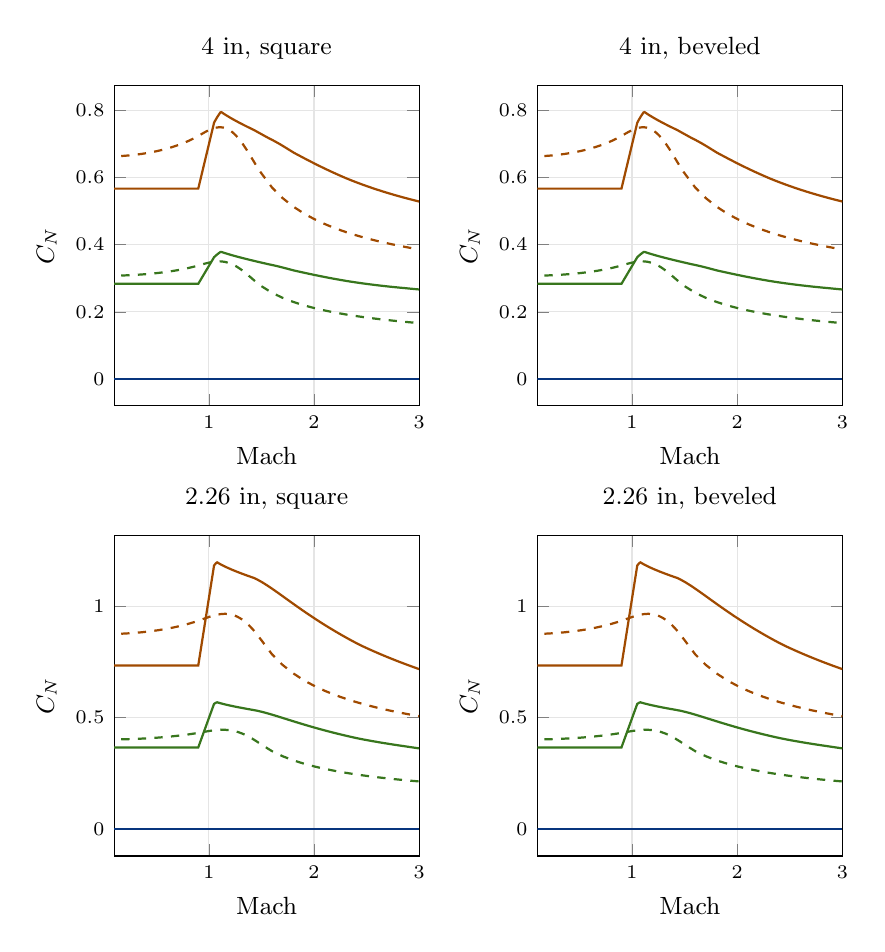
\begin{tikzpicture}
\begin{groupplot}[group style={group size=2 by 2,horizontal sep=1.50cm,vertical sep=1.65cm},width=.45\textwidth,height=5.65cm,grid=major,grid style={gray!20},tick label style={font=\scriptsize},label style={font=\small},title style={font=\small},scaled y ticks=false,yticklabel style={/pgf/number format/fixed,/pgf/number format/precision=3},unbounded coords=jump]
\nextgroupplot[title={4 in, square},xlabel={Mach},ylabel={$C_N$},xmin=0.1,xmax=3]
\addplot[thick,B,dashed] coordinates {(0.01,0) (0.06,0) (0.11,0) (0.16,0) (0.21,0) (0.26,0) (0.31,0) (0.36,0) (0.41,0) (0.46,0) (0.51,0) (0.56,0) (0.61,0) (0.66,0) (0.71,0) (0.76,0) (0.81,0) (0.86,0) (0.91,0) (0.96,0) (1.01,0) (1.06,0) (1.11,0) (1.16,0) (1.21,0) (1.26,0) (1.31,0) (1.36,0) (1.41,0) (1.46,0) (1.51,0) (1.56,0) (1.61,0) (1.66,0) (1.71,0) (1.76,0) (1.81,0) (1.86,0) (1.91,0) (1.96,0) (2.01,0) (2.06,0) (2.11,0) (2.16,0) (2.21,0) (2.26,0) (2.31,0) (2.36,0) (2.41,0) (2.46,0) (2.51,0) (2.56,0) (2.61,0) (2.66,0) (2.71,0) (2.76,0) (2.81,0) (2.86,0) (2.91,0) (2.96,0) (3,0)};
\addplot[thick,B] coordinates {(0.01,0) (0.06,0) (0.11,0) (0.16,0) (0.21,0) (0.26,0) (0.31,0) (0.36,0) (0.41,0) (0.46,0) (0.51,0) (0.56,0) (0.61,0) (0.66,0) (0.71,0) (0.76,0) (0.81,0) (0.86,0) (0.91,0) (0.96,0) (1.01,0) (1.06,0) (1.11,0) (1.16,0) (1.21,0) (1.26,0) (1.31,0) (1.36,0) (1.41,0) (1.46,0) (1.51,0) (1.56,0) (1.61,0) (1.66,0) (1.71,0) (1.76,0) (1.81,0) (1.86,0) (1.91,0) (1.96,0) (2.01,0) (2.06,0) (2.11,0) (2.16,0) (2.21,0) (2.26,0) (2.31,0) (2.36,0) (2.41,0) (2.46,0) (2.51,0) (2.56,0) (2.61,0) (2.66,0) (2.71,0) (2.76,0) (2.81,0) (2.86,0) (2.91,0) (2.96,0) (3,0)};
\addplot[thick,g,dashed] coordinates {(0.01,0.3074475) (0.06,0.307551) (0.11,0.3078032) (0.16,0.308206) (0.21,0.3087625) (0.26,0.3094773) (0.31,0.3103563) (0.36,0.3114068) (0.41,0.312638) (0.46,0.3140611) (0.51,0.3156897) (0.56,0.31754) (0.61,0.3196318) (0.66,0.3219888) (0.71,0.32464) (0.76,0.3276205) (0.81,0.330974) (0.86,0.3347548) (0.91,0.3390287) (0.96,0.3435422) (1.01,0.3474598) (1.04,0.349187) (1.06,0.3499836) (1.1,0.3505511) (1.11,0.3504552) (1.14,0.3495435) (1.16,0.3483905) (1.19,0.3458099) (1.21,0.3435139) (1.23,0.3407595) (1.26,0.3357922) (1.28,0.3319514) (1.31,0.3254692) (1.33,0.3207247) (1.36,0.3130998) (1.41,0.2995843) (1.46,0.2862026) (1.49,0.278924) (1.51,0.2747616) (1.56,0.2649854) (1.6,0.2571644) (1.61,0.2556562) (1.66,0.2481153) (1.7,0.2420826) (1.71,0.2408722) (1.76,0.2348202) (1.81,0.2289792) (1.86,0.2239819) (1.91,0.2191408) (1.96,0.2149246) (2.01,0.2108281) (2.06,0.2072104) (2.11,0.2036869) (2.16,0.2005402) (2.21,0.1974694) (2.26,0.1947015) (2.31,0.1919958) (2.36,0.1895381) (2.41,0.187132) (2.46,0.1849322) (2.51,0.1827759) (2.56,0.1807931) (2.61,0.1788474) (2.66,0.1770495) (2.71,0.1752833) (2.76,0.1736443) (2.81,0.1720328) (2.86,0.1705315) (2.91,0.1690542) (2.96,0.1676732) (3,0.1665684)};
\addplot[thick,g] coordinates {(0.01,0.2835582) (0.06,0.2835582) (0.11,0.2835582) (0.16,0.2835582) (0.21,0.2835582) (0.26,0.2835582) (0.31,0.2835582) (0.36,0.2835582) (0.41,0.2835582) (0.46,0.2835582) (0.51,0.2835582) (0.56,0.2835582) (0.61,0.2835582) (0.66,0.2835582) (0.71,0.2835582) (0.76,0.2835582) (0.81,0.2835582) (0.86,0.2835582) (0.9,0.2835582) (0.91,0.2888339) (0.96,0.3152124) (1.01,0.3415909) (1.05,0.3626936) (1.06,0.3657319) (1.08,0.3711638) (1.09,0.373641) (1.11,0.3782451) (1.12,0.3786541) (1.16,0.3744859) (1.21,0.3697616) (1.26,0.3653874) (1.31,0.3612514) (1.36,0.357287) (1.41,0.3534505) (1.46,0.349712) (1.51,0.34605) (1.56,0.342448) (1.61,0.339102) (1.66,0.3355376) (1.71,0.3315827) (1.76,0.327418) (1.81,0.3232781) (1.86,0.3198089) (1.91,0.3163673) (1.96,0.3129871) (2.01,0.3096896) (2.06,0.3064882) (2.11,0.3033902) (2.16,0.3003989) (2.21,0.2975151) (2.26,0.2947374) (2.31,0.2920637) (2.36,0.2895863) (2.41,0.2872567) (2.46,0.2850418) (2.51,0.2829372) (2.56,0.2809384) (2.61,0.2790406) (2.66,0.2772398) (2.71,0.2755313) (2.76,0.2739112) (2.81,0.2723755) (2.86,0.2709204) (2.91,0.269387) (2.96,0.2679084) (3,0.2667762)};
\addplot[thick,burntorange,dashed] coordinates {(0.01,0.662495) (0.06,0.662702) (0.11,0.6632063) (0.16,0.6640118) (0.21,0.6651249) (0.26,0.6665546) (0.31,0.6683125) (0.36,0.6704135) (0.41,0.6728759) (0.46,0.6757221) (0.51,0.6789793) (0.56,0.6826799) (0.61,0.6868635) (0.66,0.6915776) (0.71,0.6968798) (0.76,0.7028409) (0.81,0.7095479) (0.86,0.7171095) (0.91,0.7256575) (0.96,0.7347275) (1.01,0.7427683) (1.04,0.7464644) (1.06,0.748277) (1.1,0.7500019) (1.11,0.74999) (1.14,0.7487832) (1.16,0.7469512) (1.19,0.7425881) (1.21,0.7385807) (1.23,0.7336929) (1.26,0.7247434) (1.28,0.7177436) (1.31,0.7058172) (1.33,0.6970156) (1.36,0.6827615) (1.41,0.657186) (1.46,0.6314187) (1.49,0.6171275) (1.51,0.6085505) (1.56,0.5876421) (1.6,0.5709154) (1.61,0.5677571) (1.66,0.5519654) (1.7,0.539332) (1.71,0.5368292) (1.76,0.5243155) (1.81,0.5122549) (1.86,0.5020069) (1.91,0.4920892) (1.96,0.4834924) (2.01,0.4751459) (2.06,0.4678001) (2.11,0.4606497) (2.16,0.4542806) (2.21,0.4480677) (2.26,0.4424793) (2.31,0.4370182) (2.36,0.4320662) (2.41,0.4272195) (2.46,0.4227945) (2.51,0.418458) (2.56,0.4144754) (2.61,0.410568) (2.66,0.4069612) (2.71,0.403419) (2.76,0.4001347) (2.81,0.3969062) (2.86,0.393901) (2.91,0.3909445) (2.96,0.3881828) (3,0.3859734)};
\addplot[thick,burntorange] coordinates {(0.01,0.5671165) (0.06,0.5671165) (0.11,0.5671165) (0.16,0.5671165) (0.21,0.5671165) (0.26,0.5671165) (0.31,0.5671165) (0.36,0.5671165) (0.41,0.5671165) (0.46,0.5671165) (0.51,0.5671165) (0.56,0.5671165) (0.61,0.5671165) (0.66,0.5671165) (0.71,0.5671165) (0.76,0.5671165) (0.81,0.5671165) (0.86,0.5671165) (0.9,0.5671165) (0.91,0.5801775) (0.96,0.6454826) (1.01,0.7107877) (1.05,0.7630318) (1.06,0.7691083) (1.08,0.7799721) (1.11,0.7941347) (1.12,0.7949527) (1.16,0.7866162) (1.21,0.7771677) (1.26,0.7684193) (1.31,0.7601473) (1.36,0.7522184) (1.41,0.7445455) (1.43,0.741534) (1.46,0.7363348) (1.51,0.7276231) (1.56,0.7190316) (1.61,0.7109518) (1.66,0.7024354) (1.71,0.6931381) (1.76,0.683421) (1.81,0.6737537) (1.86,0.6654277) (1.91,0.6571568) (1.96,0.6490087) (2.01,0.6410262) (2.06,0.6332358) (2.11,0.6256521) (2.16,0.6182819) (2.21,0.6111267) (2.26,0.6041838) (2.31,0.5974487) (2.36,0.5911064) (2.41,0.5850594) (2.46,0.5792421) (2.51,0.5736452) (2.56,0.56826) (2.61,0.563077) (2.66,0.5580877) (2.71,0.5532831) (2.76,0.5486553) (2.81,0.5441962) (2.86,0.5398984) (2.91,0.5357542) (2.96,0.531757) (3,0.5286606)};
\nextgroupplot[title={4 in, beveled},xlabel={Mach},ylabel={$C_N$},xmin=0.1,xmax=3]
\addplot[thick,B,dashed] coordinates {(0.01,0) (0.06,0) (0.11,0) (0.16,0) (0.21,0) (0.26,0) (0.31,0) (0.36,0) (0.41,0) (0.46,0) (0.51,0) (0.56,0) (0.61,0) (0.66,0) (0.71,0) (0.76,0) (0.81,0) (0.86,0) (0.91,0) (0.96,0) (1.01,0) (1.06,0) (1.11,0) (1.16,0) (1.21,0) (1.26,0) (1.31,0) (1.36,0) (1.41,0) (1.46,0) (1.51,0) (1.56,0) (1.61,0) (1.66,0) (1.71,0) (1.76,0) (1.81,0) (1.86,0) (1.91,0) (1.96,0) (2.01,0) (2.06,0) (2.11,0) (2.16,0) (2.21,0) (2.26,0) (2.31,0) (2.36,0) (2.41,0) (2.46,0) (2.51,0) (2.56,0) (2.61,0) (2.66,0) (2.71,0) (2.76,0) (2.81,0) (2.86,0) (2.91,0) (2.96,0) (3,0)};
\addplot[thick,B] coordinates {(0.01,0) (0.06,0) (0.11,0) (0.16,0) (0.21,0) (0.26,0) (0.31,0) (0.36,0) (0.41,0) (0.46,0) (0.51,0) (0.56,0) (0.61,0) (0.66,0) (0.71,0) (0.76,0) (0.81,0) (0.86,0) (0.91,0) (0.96,0) (1.01,0) (1.06,0) (1.11,0) (1.16,0) (1.21,0) (1.26,0) (1.31,0) (1.36,0) (1.41,0) (1.46,0) (1.51,0) (1.56,0) (1.61,0) (1.66,0) (1.71,0) (1.76,0) (1.81,0) (1.86,0) (1.91,0) (1.96,0) (2.01,0) (2.06,0) (2.11,0) (2.16,0) (2.21,0) (2.26,0) (2.31,0) (2.36,0) (2.41,0) (2.46,0) (2.51,0) (2.56,0) (2.61,0) (2.66,0) (2.71,0) (2.76,0) (2.81,0) (2.86,0) (2.91,0) (2.96,0) (3,0)};
\addplot[thick,g,dashed] coordinates {(0.01,0.3074475) (0.06,0.307551) (0.11,0.3078032) (0.16,0.308206) (0.21,0.3087625) (0.26,0.3094773) (0.31,0.3103563) (0.36,0.3114068) (0.41,0.312638) (0.46,0.3140611) (0.51,0.3156897) (0.56,0.31754) (0.61,0.3196318) (0.66,0.3219888) (0.71,0.32464) (0.76,0.3276205) (0.81,0.330974) (0.86,0.3347548) (0.91,0.3390287) (0.96,0.3435422) (1.01,0.3474598) (1.04,0.349187) (1.06,0.3499836) (1.1,0.3505511) (1.11,0.3504552) (1.14,0.3495435) (1.16,0.3483905) (1.19,0.3458099) (1.21,0.3435139) (1.23,0.3407595) (1.26,0.3357922) (1.28,0.3319514) (1.31,0.3254692) (1.33,0.3207247) (1.36,0.3130998) (1.41,0.2995843) (1.46,0.2862026) (1.49,0.278924) (1.51,0.2747616) (1.56,0.2649854) (1.6,0.2571644) (1.61,0.2556562) (1.66,0.2481153) (1.7,0.2420826) (1.71,0.2408722) (1.76,0.2348202) (1.81,0.2289792) (1.86,0.2239819) (1.91,0.2191408) (1.96,0.2149246) (2.01,0.2108281) (2.06,0.2072104) (2.11,0.2036869) (2.16,0.2005402) (2.21,0.1974694) (2.26,0.1947015) (2.31,0.1919958) (2.36,0.1895381) (2.41,0.187132) (2.46,0.1849322) (2.51,0.1827759) (2.56,0.1807931) (2.61,0.1788474) (2.66,0.1770495) (2.71,0.1752833) (2.76,0.1736443) (2.81,0.1720328) (2.86,0.1705315) (2.91,0.1690542) (2.96,0.1676732) (3,0.1665684)};
\addplot[thick,g] coordinates {(0.01,0.2835582) (0.06,0.2835582) (0.11,0.2835582) (0.16,0.2835582) (0.21,0.2835582) (0.26,0.2835582) (0.31,0.2835582) (0.36,0.2835582) (0.41,0.2835582) (0.46,0.2835582) (0.51,0.2835582) (0.56,0.2835582) (0.61,0.2835582) (0.66,0.2835582) (0.71,0.2835582) (0.76,0.2835582) (0.81,0.2835582) (0.86,0.2835582) (0.9,0.2835582) (0.91,0.2888339) (0.96,0.3152124) (1.01,0.3415909) (1.05,0.3626936) (1.06,0.3657319) (1.08,0.3711638) (1.09,0.373641) (1.11,0.3782451) (1.12,0.3786541) (1.16,0.3744859) (1.21,0.3697616) (1.26,0.3653874) (1.31,0.3612514) (1.36,0.357287) (1.41,0.3534505) (1.46,0.349712) (1.51,0.34605) (1.56,0.342448) (1.61,0.339102) (1.66,0.3355376) (1.71,0.3315827) (1.76,0.327418) (1.81,0.3232781) (1.86,0.3198089) (1.91,0.3163673) (1.96,0.3129871) (2.01,0.3096896) (2.06,0.3064882) (2.11,0.3033902) (2.16,0.3003989) (2.21,0.2975151) (2.26,0.2947374) (2.31,0.2920637) (2.36,0.2895863) (2.41,0.2872567) (2.46,0.2850418) (2.51,0.2829372) (2.56,0.2809384) (2.61,0.2790406) (2.66,0.2772398) (2.71,0.2755313) (2.76,0.2739112) (2.81,0.2723755) (2.86,0.2709204) (2.91,0.269387) (2.96,0.2679084) (3,0.2667762)};
\addplot[thick,burntorange,dashed] coordinates {(0.01,0.662495) (0.06,0.662702) (0.11,0.6632063) (0.16,0.6640118) (0.21,0.6651249) (0.26,0.6665546) (0.31,0.6683125) (0.36,0.6704135) (0.41,0.6728759) (0.46,0.6757221) (0.51,0.6789793) (0.56,0.6826799) (0.61,0.6868635) (0.66,0.6915776) (0.71,0.6968798) (0.76,0.7028409) (0.81,0.7095479) (0.86,0.7171095) (0.91,0.7256575) (0.96,0.7347275) (1.01,0.7427683) (1.04,0.7464644) (1.06,0.748277) (1.1,0.7500019) (1.11,0.74999) (1.14,0.7487832) (1.16,0.7469512) (1.19,0.7425881) (1.21,0.7385807) (1.23,0.7336929) (1.26,0.7247434) (1.28,0.7177436) (1.31,0.7058172) (1.33,0.6970156) (1.36,0.6827615) (1.41,0.657186) (1.46,0.6314187) (1.49,0.6171275) (1.51,0.6085505) (1.56,0.5876421) (1.6,0.5709154) (1.61,0.5677571) (1.66,0.5519654) (1.7,0.539332) (1.71,0.5368292) (1.76,0.5243155) (1.81,0.5122549) (1.86,0.5020069) (1.91,0.4920892) (1.96,0.4834924) (2.01,0.4751459) (2.06,0.4678001) (2.11,0.4606497) (2.16,0.4542806) (2.21,0.4480677) (2.26,0.4424793) (2.31,0.4370182) (2.36,0.4320662) (2.41,0.4272195) (2.46,0.4227945) (2.51,0.418458) (2.56,0.4144754) (2.61,0.410568) (2.66,0.4069612) (2.71,0.403419) (2.76,0.4001347) (2.81,0.3969062) (2.86,0.393901) (2.91,0.3909445) (2.96,0.3881828) (3,0.3859734)};
\addplot[thick,burntorange] coordinates {(0.01,0.5671165) (0.06,0.5671165) (0.11,0.5671165) (0.16,0.5671165) (0.21,0.5671165) (0.26,0.5671165) (0.31,0.5671165) (0.36,0.5671165) (0.41,0.5671165) (0.46,0.5671165) (0.51,0.5671165) (0.56,0.5671165) (0.61,0.5671165) (0.66,0.5671165) (0.71,0.5671165) (0.76,0.5671165) (0.81,0.5671165) (0.86,0.5671165) (0.9,0.5671165) (0.91,0.5801775) (0.96,0.6454826) (1.01,0.7107877) (1.05,0.7630318) (1.06,0.7691083) (1.08,0.7799721) (1.11,0.7941347) (1.12,0.7949527) (1.16,0.7866162) (1.21,0.7771677) (1.26,0.7684193) (1.31,0.7601473) (1.36,0.7522184) (1.41,0.7445455) (1.43,0.741534) (1.46,0.7363348) (1.51,0.7276231) (1.56,0.7190316) (1.61,0.7109518) (1.66,0.7024354) (1.71,0.6931381) (1.76,0.683421) (1.81,0.6737537) (1.86,0.6654277) (1.91,0.6571568) (1.96,0.6490087) (2.01,0.6410262) (2.06,0.6332358) (2.11,0.6256521) (2.16,0.6182819) (2.21,0.6111267) (2.26,0.6041838) (2.31,0.5974487) (2.36,0.5911064) (2.41,0.5850594) (2.46,0.5792421) (2.51,0.5736452) (2.56,0.56826) (2.61,0.563077) (2.66,0.5580877) (2.71,0.5532831) (2.76,0.5486553) (2.81,0.5441962) (2.86,0.5398984) (2.91,0.5357542) (2.96,0.531757) (3,0.5286606)};
\nextgroupplot[title={2.26 in, square},xlabel={Mach},ylabel={$C_N$},xmin=0.1,xmax=3]
\addplot[thick,B,dashed] coordinates {(0.01,0) (0.06,0) (0.11,0) (0.16,0) (0.21,0) (0.26,0) (0.31,0) (0.36,0) (0.41,0) (0.46,0) (0.51,0) (0.56,0) (0.61,0) (0.66,0) (0.71,0) (0.76,0) (0.81,0) (0.86,0) (0.91,0) (0.96,0) (1.01,0) (1.06,0) (1.11,0) (1.16,0) (1.21,0) (1.26,0) (1.31,0) (1.36,0) (1.41,0) (1.46,0) (1.51,0) (1.56,0) (1.61,0) (1.66,0) (1.71,0) (1.76,0) (1.81,0) (1.86,0) (1.91,0) (1.96,0) (2.01,0) (2.06,0) (2.11,0) (2.16,0) (2.21,0) (2.26,0) (2.31,0) (2.36,0) (2.41,0) (2.46,0) (2.51,0) (2.56,0) (2.61,0) (2.66,0) (2.71,0) (2.76,0) (2.81,0) (2.86,0) (2.91,0) (2.96,0) (3,0)};
\addplot[thick,B] coordinates {(0.01,0) (0.06,0) (0.11,0) (0.16,0) (0.21,0) (0.26,0) (0.31,0) (0.36,0) (0.41,0) (0.46,0) (0.51,0) (0.56,0) (0.61,0) (0.66,0) (0.71,0) (0.76,0) (0.81,0) (0.86,0) (0.91,0) (0.96,0) (1.01,0) (1.06,0) (1.11,0) (1.16,0) (1.21,0) (1.26,0) (1.31,0) (1.36,0) (1.41,0) (1.46,0) (1.51,0) (1.56,0) (1.61,0) (1.66,0) (1.71,0) (1.76,0) (1.81,0) (1.86,0) (1.91,0) (1.96,0) (2.01,0) (2.06,0) (2.11,0) (2.16,0) (2.21,0) (2.26,0) (2.31,0) (2.36,0) (2.41,0) (2.46,0) (2.51,0) (2.56,0) (2.61,0) (2.66,0) (2.71,0) (2.76,0) (2.81,0) (2.86,0) (2.91,0) (2.96,0) (3,0)};
\addplot[thick,g,dashed] coordinates {(0.01,0.4022197) (0.06,0.4023277) (0.11,0.4025904) (0.16,0.4030096) (0.21,0.4035876) (0.26,0.4043281) (0.31,0.4052356) (0.36,0.4063158) (0.41,0.4075757) (0.46,0.4090238) (0.51,0.4106701) (0.56,0.4125265) (0.61,0.4146068) (0.66,0.4169277) (0.71,0.4195084) (0.76,0.4223721) (0.81,0.425546) (0.86,0.4290627) (0.91,0.432961) (0.96,0.4371304) (1.01,0.4410541) (1.06,0.4441509) (1.11,0.4458661) (1.13,0.4460514) (1.16,0.4457028) (1.19,0.4445286) (1.21,0.4432525) (1.24,0.4405585) (1.26,0.4382263) (1.28,0.4354579) (1.31,0.4304862) (1.33,0.4266332) (1.36,0.4200756) (1.38,0.4152131) (1.41,0.4072507) (1.46,0.3925113) (1.51,0.376916) (1.56,0.3622362) (1.6,0.3504923) (1.61,0.3482276) (1.66,0.3369043) (1.7,0.3278457) (1.71,0.3260282) (1.76,0.3169406) (1.8,0.3096706) (1.81,0.3081698) (1.86,0.3006659) (1.91,0.2933965) (1.96,0.2870655) (2.01,0.2809143) (2.06,0.275482) (2.11,0.2701912) (2.16,0.2654662) (2.21,0.260855) (2.26,0.2566989) (2.31,0.2526359) (2.36,0.2489455) (2.41,0.2453326) (2.46,0.2420294) (2.51,0.2387914) (2.56,0.2358142) (2.61,0.2328924) (2.66,0.2301927) (2.71,0.2275407) (2.76,0.2250795) (2.81,0.2226597) (2.86,0.2204054) (2.91,0.2181872) (2.96,0.2161135) (3,0.2144545)};
\addplot[thick,g] coordinates {(0.01,0.3669943) (0.06,0.3669943) (0.11,0.3669943) (0.16,0.3669943) (0.21,0.3669943) (0.26,0.3669943) (0.31,0.3669943) (0.36,0.3669943) (0.41,0.3669943) (0.46,0.3669943) (0.51,0.3669943) (0.56,0.3669943) (0.61,0.3669943) (0.66,0.3669943) (0.71,0.3669943) (0.76,0.3669943) (0.81,0.3669943) (0.86,0.3669943) (0.9,0.3669943) (0.91,0.3799918) (0.96,0.444979) (1.01,0.5099662) (1.05,0.561956) (1.06,0.5649534) (1.07,0.5677262) (1.08,0.5691256) (1.11,0.5649888) (1.16,0.559011) (1.21,0.5537182) (1.26,0.548856) (1.31,0.5442914) (1.36,0.5399449) (1.41,0.5357647) (1.46,0.5313697) (1.51,0.5258248) (1.56,0.5194518) (1.61,0.5125434) (1.66,0.5053216) (1.71,0.4979489) (1.76,0.4905418) (1.81,0.4831825) (1.86,0.4759281) (1.91,0.4688179) (1.96,0.4618772) (2.01,0.4551224) (2.06,0.448563) (2.11,0.442203) (2.16,0.436043) (2.21,0.4300814) (2.26,0.4243145) (2.31,0.4187372) (2.36,0.4133439) (2.41,0.4081284) (2.46,0.4034046) (2.51,0.3990226) (2.56,0.3947965) (2.61,0.3907199) (2.66,0.3867864) (2.71,0.38299) (2.76,0.3793242) (2.81,0.3757835) (2.86,0.3723624) (2.91,0.3688169) (2.96,0.3653517) (3,0.3626548)};
\addplot[thick,burntorange,dashed] coordinates {(0.01,0.8746562) (0.06,0.8748721) (0.11,0.8753976) (0.16,0.8762359) (0.21,0.8773921) (0.26,0.878873) (0.31,0.880688) (0.36,0.8828484) (0.41,0.8853683) (0.46,0.8882645) (0.51,0.891557) (0.56,0.8952697) (0.61,0.8994304) (0.66,0.9040721) (0.71,0.9092337) (0.76,0.914961) (0.81,0.9213088) (0.86,0.9283421) (0.91,0.9361391) (0.96,0.9445425) (1.01,0.9526984) (1.06,0.9595845) (1.11,0.9641709) (1.15,0.9655251) (1.16,0.9654818) (1.19,0.9643318) (1.21,0.9626576) (1.24,0.9586856) (1.26,0.955017) (1.29,0.9479255) (1.31,0.9421191) (1.33,0.9354452) (1.36,0.9238251) (1.38,0.9150335) (1.41,0.9003607) (1.43,0.8896576) (1.46,0.872378) (1.51,0.8412081) (1.56,0.8098123) (1.6,0.7846958) (1.61,0.7799532) (1.66,0.7562406) (1.7,0.7372704) (1.71,0.7335123) (1.76,0.7147218) (1.8,0.6996894) (1.81,0.6966118) (1.86,0.6812236) (1.91,0.6663312) (1.96,0.6534224) (2.01,0.6408893) (2.06,0.6298591) (2.11,0.6191221) (2.16,0.6095583) (2.21,0.6002291) (2.26,0.5918376) (2.31,0.5836373) (2.36,0.5762014) (2.41,0.5689237) (2.46,0.5622792) (2.51,0.5557675) (2.56,0.5497873) (2.61,0.54392) (2.66,0.5385042) (2.71,0.5331851) (2.76,0.5282535) (2.81,0.5234056) (2.86,0.5188931) (2.91,0.5144536) (2.96,0.5103067) (3,0.5069892)};
\addplot[thick,burntorange] coordinates {(0.01,0.7339886) (0.06,0.7339886) (0.11,0.7339886) (0.16,0.7339886) (0.21,0.7339886) (0.26,0.7339886) (0.31,0.7339886) (0.36,0.7339886) (0.41,0.7339886) (0.46,0.7339886) (0.51,0.7339886) (0.56,0.7339886) (0.61,0.7339886) (0.66,0.7339886) (0.71,0.7339886) (0.76,0.7339886) (0.81,0.7339886) (0.86,0.7339886) (0.9,0.7339886) (0.91,0.7638429) (0.96,0.9131143) (1.01,1.062386) (1.05,1.181803) (1.06,1.187797) (1.07,1.193343) (1.08,1.196142) (1.11,1.187868) (1.16,1.175913) (1.21,1.165327) (1.26,1.155603) (1.31,1.146473) (1.36,1.13778) (1.41,1.12942) (1.43,1.126196) (1.46,1.119502) (1.51,1.106278) (1.56,1.091398) (1.61,1.075447) (1.66,1.05887) (1.71,1.04199) (1.76,1.025042) (1.81,1.00819) (1.86,0.9915472) (1.91,0.9751928) (1.96,0.9591775) (2.01,0.943534) (2.06,0.9282813) (2.11,0.9134274) (2.16,0.8989735) (2.21,0.8849165) (2.26,0.8712487) (2.31,0.8579603) (2.36,0.8450397) (2.41,0.8324748) (2.46,0.8208934) (2.51,0.8099956) (2.56,0.7994094) (2.61,0.7891224) (2.66,0.7791214) (2.71,0.7693946) (2.76,0.7599292) (2.81,0.7507139) (2.86,0.7417378) (2.91,0.73299) (2.96,0.7244602) (3,0.7177867)};
\nextgroupplot[title={2.26 in, beveled},xlabel={Mach},ylabel={$C_N$},xmin=0.1,xmax=3]
\addplot[thick,B,dashed] coordinates {(0.01,0) (0.06,0) (0.11,0) (0.16,0) (0.21,0) (0.26,0) (0.31,0) (0.36,0) (0.41,0) (0.46,0) (0.51,0) (0.56,0) (0.61,0) (0.66,0) (0.71,0) (0.76,0) (0.81,0) (0.86,0) (0.91,0) (0.96,0) (1.01,0) (1.06,0) (1.11,0) (1.16,0) (1.21,0) (1.26,0) (1.31,0) (1.36,0) (1.41,0) (1.46,0) (1.51,0) (1.56,0) (1.61,0) (1.66,0) (1.71,0) (1.76,0) (1.81,0) (1.86,0) (1.91,0) (1.96,0) (2.01,0) (2.06,0) (2.11,0) (2.16,0) (2.21,0) (2.26,0) (2.31,0) (2.36,0) (2.41,0) (2.46,0) (2.51,0) (2.56,0) (2.61,0) (2.66,0) (2.71,0) (2.76,0) (2.81,0) (2.86,0) (2.91,0) (2.96,0) (3,0)};
\addplot[thick,B] coordinates {(0.01,0) (0.06,0) (0.11,0) (0.16,0) (0.21,0) (0.26,0) (0.31,0) (0.36,0) (0.41,0) (0.46,0) (0.51,0) (0.56,0) (0.61,0) (0.66,0) (0.71,0) (0.76,0) (0.81,0) (0.86,0) (0.91,0) (0.96,0) (1.01,0) (1.06,0) (1.11,0) (1.16,0) (1.21,0) (1.26,0) (1.31,0) (1.36,0) (1.41,0) (1.46,0) (1.51,0) (1.56,0) (1.61,0) (1.66,0) (1.71,0) (1.76,0) (1.81,0) (1.86,0) (1.91,0) (1.96,0) (2.01,0) (2.06,0) (2.11,0) (2.16,0) (2.21,0) (2.26,0) (2.31,0) (2.36,0) (2.41,0) (2.46,0) (2.51,0) (2.56,0) (2.61,0) (2.66,0) (2.71,0) (2.76,0) (2.81,0) (2.86,0) (2.91,0) (2.96,0) (3,0)};
\addplot[thick,g,dashed] coordinates {(0.01,0.4022197) (0.06,0.4023277) (0.11,0.4025904) (0.16,0.4030096) (0.21,0.4035876) (0.26,0.4043281) (0.31,0.4052356) (0.36,0.4063158) (0.41,0.4075757) (0.46,0.4090238) (0.51,0.4106701) (0.56,0.4125265) (0.61,0.4146068) (0.66,0.4169277) (0.71,0.4195084) (0.76,0.4223721) (0.81,0.425546) (0.86,0.4290627) (0.91,0.432961) (0.96,0.4371304) (1.01,0.4410541) (1.06,0.4441509) (1.11,0.4458661) (1.13,0.4460514) (1.16,0.4457028) (1.19,0.4445286) (1.21,0.4432525) (1.24,0.4405585) (1.26,0.4382263) (1.28,0.4354579) (1.31,0.4304862) (1.33,0.4266332) (1.36,0.4200756) (1.38,0.4152131) (1.41,0.4072507) (1.46,0.3925113) (1.51,0.376916) (1.56,0.3622362) (1.6,0.3504923) (1.61,0.3482276) (1.66,0.3369043) (1.7,0.3278457) (1.71,0.3260282) (1.76,0.3169406) (1.8,0.3096706) (1.81,0.3081698) (1.86,0.3006659) (1.91,0.2933965) (1.96,0.2870655) (2.01,0.2809143) (2.06,0.275482) (2.11,0.2701912) (2.16,0.2654662) (2.21,0.260855) (2.26,0.2566989) (2.31,0.2526359) (2.36,0.2489455) (2.41,0.2453326) (2.46,0.2420294) (2.51,0.2387914) (2.56,0.2358142) (2.61,0.2328924) (2.66,0.2301927) (2.71,0.2275407) (2.76,0.2250795) (2.81,0.2226597) (2.86,0.2204054) (2.91,0.2181872) (2.96,0.2161135) (3,0.2144545)};
\addplot[thick,g] coordinates {(0.01,0.3669943) (0.06,0.3669943) (0.11,0.3669943) (0.16,0.3669943) (0.21,0.3669943) (0.26,0.3669943) (0.31,0.3669943) (0.36,0.3669943) (0.41,0.3669943) (0.46,0.3669943) (0.51,0.3669943) (0.56,0.3669943) (0.61,0.3669943) (0.66,0.3669943) (0.71,0.3669943) (0.76,0.3669943) (0.81,0.3669943) (0.86,0.3669943) (0.9,0.3669943) (0.91,0.3799918) (0.96,0.444979) (1.01,0.5099662) (1.05,0.561956) (1.06,0.5649534) (1.07,0.5677262) (1.08,0.5691256) (1.11,0.5649888) (1.16,0.559011) (1.21,0.5537182) (1.26,0.548856) (1.31,0.5442914) (1.36,0.5399449) (1.41,0.5357647) (1.46,0.5313697) (1.51,0.5258248) (1.56,0.5194518) (1.61,0.5125434) (1.66,0.5053216) (1.71,0.4979489) (1.76,0.4905418) (1.81,0.4831825) (1.86,0.4759281) (1.91,0.4688179) (1.96,0.4618772) (2.01,0.4551224) (2.06,0.448563) (2.11,0.442203) (2.16,0.436043) (2.21,0.4300814) (2.26,0.4243145) (2.31,0.4187372) (2.36,0.4133439) (2.41,0.4081284) (2.46,0.4034046) (2.51,0.3990226) (2.56,0.3947965) (2.61,0.3907199) (2.66,0.3867864) (2.71,0.38299) (2.76,0.3793242) (2.81,0.3757835) (2.86,0.3723624) (2.91,0.3688169) (2.96,0.3653517) (3,0.3626548)};
\addplot[thick,burntorange,dashed] coordinates {(0.01,0.8746562) (0.06,0.8748721) (0.11,0.8753976) (0.16,0.8762359) (0.21,0.8773921) (0.26,0.878873) (0.31,0.880688) (0.36,0.8828484) (0.41,0.8853683) (0.46,0.8882645) (0.51,0.891557) (0.56,0.8952697) (0.61,0.8994304) (0.66,0.9040721) (0.71,0.9092337) (0.76,0.914961) (0.81,0.9213088) (0.86,0.9283421) (0.91,0.9361391) (0.96,0.9445425) (1.01,0.9526984) (1.06,0.9595845) (1.11,0.9641709) (1.15,0.9655251) (1.16,0.9654818) (1.19,0.9643318) (1.21,0.9626576) (1.24,0.9586856) (1.26,0.955017) (1.29,0.9479255) (1.31,0.9421191) (1.33,0.9354452) (1.36,0.9238251) (1.38,0.9150335) (1.41,0.9003607) (1.43,0.8896576) (1.46,0.872378) (1.51,0.8412081) (1.56,0.8098123) (1.6,0.7846958) (1.61,0.7799532) (1.66,0.7562406) (1.7,0.7372704) (1.71,0.7335123) (1.76,0.7147218) (1.8,0.6996894) (1.81,0.6966118) (1.86,0.6812236) (1.91,0.6663312) (1.96,0.6534224) (2.01,0.6408893) (2.06,0.6298591) (2.11,0.6191221) (2.16,0.6095583) (2.21,0.6002291) (2.26,0.5918376) (2.31,0.5836373) (2.36,0.5762014) (2.41,0.5689237) (2.46,0.5622792) (2.51,0.5557675) (2.56,0.5497873) (2.61,0.54392) (2.66,0.5385042) (2.71,0.5331851) (2.76,0.5282535) (2.81,0.5234056) (2.86,0.5188931) (2.91,0.5144536) (2.96,0.5103067) (3,0.5069892)};
\addplot[thick,burntorange] coordinates {(0.01,0.7339886) (0.06,0.7339886) (0.11,0.7339886) (0.16,0.7339886) (0.21,0.7339886) (0.26,0.7339886) (0.31,0.7339886) (0.36,0.7339886) (0.41,0.7339886) (0.46,0.7339886) (0.51,0.7339886) (0.56,0.7339886) (0.61,0.7339886) (0.66,0.7339886) (0.71,0.7339886) (0.76,0.7339886) (0.81,0.7339886) (0.86,0.7339886) (0.9,0.7339886) (0.91,0.7638429) (0.96,0.9131143) (1.01,1.062386) (1.05,1.181803) (1.06,1.187797) (1.07,1.193343) (1.08,1.196142) (1.11,1.187868) (1.16,1.175913) (1.21,1.165327) (1.26,1.155603) (1.31,1.146473) (1.36,1.13778) (1.41,1.12942) (1.43,1.126196) (1.46,1.119502) (1.51,1.106278) (1.56,1.091398) (1.61,1.075447) (1.66,1.05887) (1.71,1.04199) (1.76,1.025042) (1.81,1.00819) (1.86,0.9915472) (1.91,0.9751928) (1.96,0.9591775) (2.01,0.943534) (2.06,0.9282813) (2.11,0.9134274) (2.16,0.8989735) (2.21,0.8849165) (2.26,0.8712487) (2.31,0.8579603) (2.36,0.8450397) (2.41,0.8324748) (2.46,0.8208934) (2.51,0.8099956) (2.56,0.7994094) (2.61,0.7891224) (2.66,0.7791214) (2.71,0.7693946) (2.76,0.7599292) (2.81,0.7507139) (2.86,0.7417378) (2.91,0.73299) (2.96,0.7244602) (3,0.7177867)};
\end{groupplot}\end{tikzpicture}
\caption{Body-axis forces are compared directly. Wind-axis drag/lift use CD=CA cos(alpha)+CN sin(alpha), CL=CN cos(alpha)-CA sin(alpha). RAS lift is reconstructed for power-off; its raw CL column corresponds to power-on when nozzle area is nonzero.}\label{fig:atlas-23-alpha-CN}
\end{figure}
\noindent{\footnotesize Export files: \code{23-alpha-CN.svg} and \code{23-alpha-CN.png}.\\ Directory: \code{aerodynamic-investigation/extended/figures/}.}

\clearpage\subsubsection*{Wind-axis lift at 0, 2 and 4 degrees}
\begin{figure}[H]\centering
{\footnotesize\begin{tabular}{lll}
\tikz[baseline=-.5ex]{\draw[thick,B,dashed] (0,0)--(.40,0);}\ MIT OR, 0 deg & \tikz[baseline=-.5ex]{\draw[thick,B] (0,0)--(.40,0);}\ RASAero, 0 deg & \tikz[baseline=-.5ex]{\draw[thick,g,dashed] (0,0)--(.40,0);}\ MIT OR, 2 deg\\
\tikz[baseline=-.5ex]{\draw[thick,g] (0,0)--(.40,0);}\ RASAero, 2 deg & \tikz[baseline=-.5ex]{\draw[thick,burntorange,dashed] (0,0)--(.40,0);}\ MIT OR, 4 deg & \tikz[baseline=-.5ex]{\draw[thick,burntorange] (0,0)--(.40,0);}\ RASAero, 4 deg\\
\end{tabular}}\par\vspace{.7em}
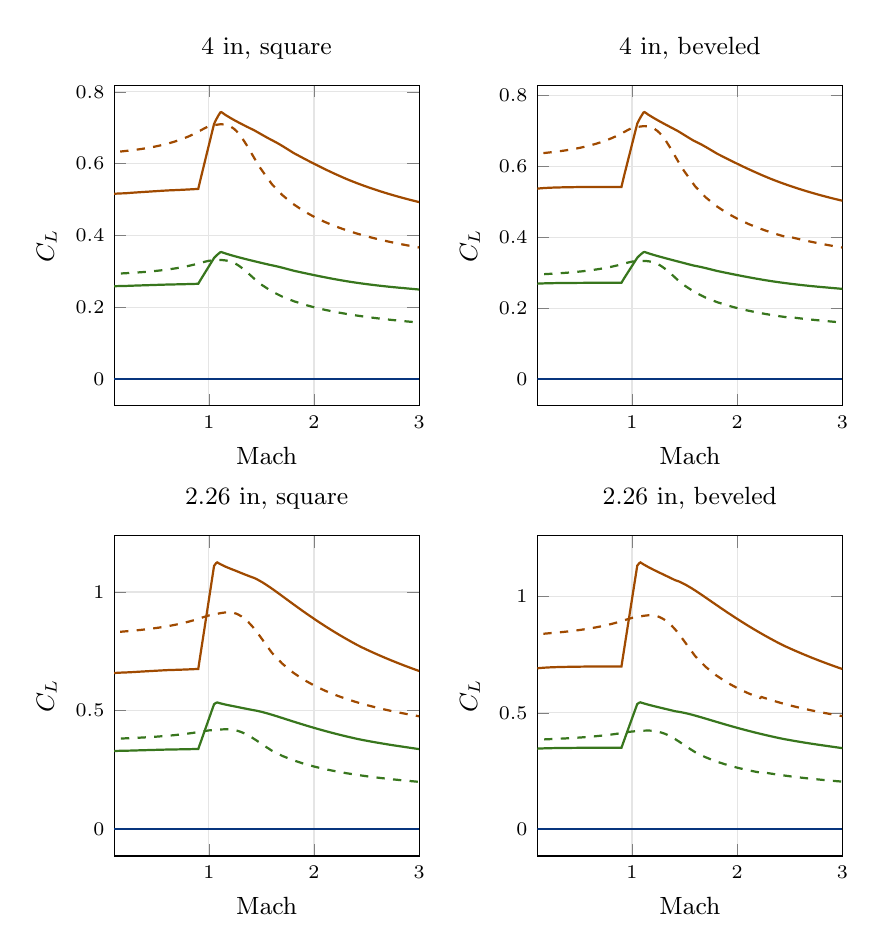
\begin{tikzpicture}
\begin{groupplot}[group style={group size=2 by 2,horizontal sep=1.50cm,vertical sep=1.65cm},width=.45\textwidth,height=5.65cm,grid=major,grid style={gray!20},tick label style={font=\scriptsize},label style={font=\small},title style={font=\small},scaled y ticks=false,yticklabel style={/pgf/number format/fixed,/pgf/number format/precision=3},unbounded coords=jump]
\nextgroupplot[title={4 in, square},xlabel={Mach},ylabel={$C_L$},xmin=0.1,xmax=3]
\addplot[thick,B,dashed] coordinates {(0.01,0) (0.06,0) (0.11,0) (0.16,0) (0.21,0) (0.26,0) (0.31,0) (0.36,0) (0.41,0) (0.46,0) (0.51,0) (0.56,0) (0.61,0) (0.66,0) (0.71,0) (0.76,0) (0.81,0) (0.86,0) (0.91,0) (0.96,0) (1.01,0) (1.06,0) (1.11,0) (1.16,0) (1.21,0) (1.26,0) (1.31,0) (1.36,0) (1.41,0) (1.46,0) (1.51,0) (1.56,0) (1.61,0) (1.66,0) (1.71,0) (1.76,0) (1.81,0) (1.86,0) (1.91,0) (1.96,0) (2.01,0) (2.06,0) (2.11,0) (2.16,0) (2.21,0) (2.26,0) (2.31,0) (2.36,0) (2.41,0) (2.46,0) (2.51,0) (2.56,0) (2.61,0) (2.66,0) (2.71,0) (2.76,0) (2.81,0) (2.86,0) (2.91,0) (2.96,0) (3,0)};
\addplot[thick,B] coordinates {(0.01,0) (0.06,0) (0.11,0) (0.16,0) (0.21,0) (0.26,0) (0.31,0) (0.36,0) (0.41,0) (0.46,0) (0.51,0) (0.56,0) (0.61,0) (0.66,0) (0.71,0) (0.76,0) (0.81,0) (0.86,0) (0.91,0) (0.96,0) (1.01,0) (1.06,0) (1.11,0) (1.16,0) (1.21,0) (1.26,0) (1.31,0) (1.36,0) (1.41,0) (1.46,0) (1.51,0) (1.56,0) (1.61,0) (1.66,0) (1.71,0) (1.76,0) (1.81,0) (1.86,0) (1.91,0) (1.96,0) (2.01,0) (2.06,0) (2.11,0) (2.16,0) (2.21,0) (2.26,0) (2.31,0) (2.36,0) (2.41,0) (2.46,0) (2.51,0) (2.56,0) (2.61,0) (2.66,0) (2.71,0) (2.76,0) (2.81,0) (2.86,0) (2.91,0) (2.96,0) (3,0)};
\addplot[thick,g,dashed] coordinates {(0.01,0.2882239) (0.02,0.2899703) (0.03,0.2908386) (0.06,0.2921523) (0.11,0.2932728) (0.16,0.2941031) (0.21,0.2948983) (0.26,0.2957405) (0.31,0.2966691) (0.36,0.2977089) (0.41,0.298879) (0.46,0.3001968) (0.51,0.3016801) (0.56,0.303348) (0.61,0.3052222) (0.66,0.3073281) (0.71,0.3096956) (0.76,0.3123608) (0.81,0.315368) (0.86,0.3187718) (0.91,0.3226337) (0.96,0.3266819) (1,0.3295051) (1.01,0.3297784) (1.06,0.3310195) (1.11,0.3315955) (1.13,0.3314015) (1.16,0.3304774) (1.19,0.3286828) (1.21,0.3269264) (1.24,0.3233964) (1.26,0.3204112) (1.28,0.3169086) (1.31,0.3107025) (1.33,0.3060892) (1.36,0.2986555) (1.41,0.2854444) (1.46,0.2723502) (1.49,0.2652364) (1.51,0.2611805) (1.56,0.251661) (1.6,0.2440365) (1.61,0.242576) (1.66,0.2352669) (1.7,0.2294121) (1.71,0.228245) (1.76,0.2224041) (1.81,0.2167652) (1.86,0.2119613) (1.91,0.2073059) (1.96,0.203268) (2.01,0.1993431) (2.06,0.1958905) (2.11,0.1925262) (2.16,0.189533) (2.21,0.1866104) (2.26,0.1839858) (2.31,0.1814185) (2.36,0.1790949) (2.41,0.1768186) (2.46,0.1747445) (2.51,0.17271) (2.56,0.1708455) (2.61,0.1690145) (2.66,0.1673279) (2.71,0.16567) (2.76,0.1641361) (2.81,0.1626268) (2.86,0.1612249) (2.91,0.1598444) (2.96,0.1585576) (3,0.1575264)};
\addplot[thick,g] coordinates {(0.01,0.2551514) (0.02,0.2564672) (0.03,0.2571199) (0.06,0.258072) (0.11,0.2587631) (0.16,0.2591347) (0.21,0.259381) (0.26,0.2600152) (0.31,0.2605105) (0.36,0.2609903) (0.41,0.2614623) (0.46,0.2619314) (0.51,0.2624007) (0.56,0.2628726) (0.61,0.2633092) (0.66,0.2636115) (0.71,0.2639393) (0.76,0.2642932) (0.81,0.2646738) (0.86,0.2650815) (0.9,0.2654276) (0.91,0.2705779) (0.92,0.2754841) (0.96,0.2944776) (1.01,0.3182377) (1.05,0.3372458) (1.06,0.3404143) (1.07,0.3433504) (1.09,0.3487076) (1.11,0.3533532) (1.12,0.3537831) (1.16,0.3497218) (1.21,0.3452649) (1.26,0.3411797) (1.31,0.3373069) (1.36,0.3335823) (1.41,0.3299639) (1.46,0.3264232) (1.51,0.3229398) (1.56,0.319498) (1.58,0.3181303) (1.61,0.3163679) (1.66,0.313087) (1.71,0.3094078) (1.76,0.3055118) (1.81,0.3016345) (1.86,0.298422) (1.91,0.2952321) (1.96,0.2920992) (2.01,0.2890368) (2.06,0.2860351) (2.11,0.2831328) (2.16,0.2803335) (2.21,0.2776381) (2.26,0.2750454) (2.31,0.2725531) (2.36,0.2702539) (2.41,0.2680991) (2.46,0.266056) (2.51,0.2641201) (2.56,0.262287) (2.61,0.2605521) (2.66,0.2589112) (2.71,0.25736) (2.76,0.2558945) (2.81,0.2545107) (2.86,0.2532051) (2.91,0.2518189) (2.96,0.2504853) (3,0.2494675)};
\addplot[thick,burntorange,dashed] coordinates {(0.01,0.6216832) (0.02,0.6252786) (0.03,0.6270656) (0.06,0.6297656) (0.11,0.6320572) (0.16,0.6337415) (0.21,0.635344) (0.26,0.6370334) (0.31,0.6388904) (0.36,0.6409655) (0.41,0.6432976) (0.46,0.6459218) (0.51,0.6488739) (0.56,0.6521922) (0.61,0.6559203) (0.66,0.6601087) (0.71,0.6648173) (0.76,0.6701184) (0.81,0.6761) (0.86,0.6828717) (0.91,0.690556) (0.96,0.6986514) (1,0.7044085) (1.01,0.7049866) (1.06,0.707844) (1.11,0.7097684) (1.12,0.7098183) (1.16,0.7086834) (1.19,0.7059462) (1.21,0.7030568) (1.24,0.6969987) (1.26,0.6917279) (1.28,0.6854368) (1.31,0.6740997) (1.33,0.6655839) (1.36,0.6517486) (1.41,0.6268451) (1.46,0.6017159) (1.49,0.5877896) (1.51,0.5794477) (1.56,0.5591067) (1.6,0.5428155) (1.61,0.5397611) (1.66,0.5244757) (1.7,0.5122319) (1.71,0.5098229) (1.76,0.4977666) (1.8,0.4881084) (1.81,0.4861441) (1.86,0.4763132) (1.91,0.466796) (1.96,0.458582) (2.01,0.4506039) (2.06,0.4436115) (2.11,0.4368019) (2.16,0.4307604) (2.21,0.4248641) (2.26,0.4195807) (2.31,0.4144148) (2.36,0.4097476) (2.41,0.405177) (2.46,0.4010188) (2.51,0.3969411) (2.56,0.3932092) (2.61,0.3895451) (2.66,0.3861742) (2.71,0.3828612) (2.76,0.3797993) (2.81,0.3767872) (2.86,0.3739922) (2.91,0.3712403) (2.96,0.3686774) (3,0.3666236)};
\addplot[thick,burntorange] coordinates {(0.01,0.5090944) (0.02,0.5117339) (0.03,0.5130434) (0.06,0.5149533) (0.11,0.5163397) (0.16,0.5170853) (0.21,0.5175794) (0.26,0.5188517) (0.31,0.5198453) (0.36,0.5208078) (0.41,0.5217546) (0.46,0.5226957) (0.51,0.5236373) (0.56,0.524584) (0.61,0.5254597) (0.66,0.5260663) (0.71,0.5267238) (0.76,0.5274337) (0.81,0.5281973) (0.86,0.5290153) (0.9,0.5297094) (0.91,0.5424936) (0.92,0.5547879) (0.96,0.6026992) (1.01,0.6626248) (1.05,0.7105652) (1.06,0.7168918) (1.07,0.7227545) (1.09,0.733452) (1.11,0.7427265) (1.12,0.743585) (1.16,0.7354782) (1.21,0.7265833) (1.26,0.7184306) (1.31,0.7107018) (1.36,0.7032684) (1.41,0.6960471) (1.43,0.6932045) (1.46,0.6882486) (1.51,0.6799119) (1.56,0.6716583) (1.61,0.6640274) (1.66,0.6560961) (1.71,0.6473695) (1.76,0.6382102) (1.81,0.6290881) (1.86,0.6212931) (1.91,0.6135432) (1.96,0.6059069) (2.01,0.5984113) (2.06,0.5910366) (2.11,0.5838603) (2.16,0.5768896) (2.21,0.5701262) (2.26,0.5635678) (2.31,0.5572099) (2.36,0.5512374) (2.41,0.5455532) (2.46,0.5400919) (2.51,0.5348446) (2.56,0.5298025) (2.61,0.5249563) (2.66,0.5202979) (2.71,0.5158184) (2.76,0.51151) (2.81,0.5073648) (2.86,0.5033755) (2.91,0.4995349) (2.96,0.4958364) (3,0.4929756)};
\nextgroupplot[title={4 in, beveled},xlabel={Mach},ylabel={$C_L$},xmin=0.1,xmax=3]
\addplot[thick,B,dashed] coordinates {(0.01,0) (0.06,0) (0.11,0) (0.16,0) (0.21,0) (0.26,0) (0.31,0) (0.36,0) (0.41,0) (0.46,0) (0.51,0) (0.56,0) (0.61,0) (0.66,0) (0.71,0) (0.76,0) (0.81,0) (0.86,0) (0.91,0) (0.96,0) (1.01,0) (1.06,0) (1.11,0) (1.16,0) (1.21,0) (1.26,0) (1.31,0) (1.36,0) (1.41,0) (1.46,0) (1.51,0) (1.56,0) (1.61,0) (1.66,0) (1.71,0) (1.76,0) (1.81,0) (1.86,0) (1.91,0) (1.96,0) (2.01,0) (2.06,0) (2.11,0) (2.16,0) (2.21,0) (2.26,0) (2.31,0) (2.36,0) (2.41,0) (2.46,0) (2.51,0) (2.56,0) (2.61,0) (2.66,0) (2.71,0) (2.76,0) (2.81,0) (2.86,0) (2.91,0) (2.96,0) (3,0)};
\addplot[thick,B] coordinates {(0.01,0) (0.06,0) (0.11,0) (0.16,0) (0.21,0) (0.26,0) (0.31,0) (0.36,0) (0.41,0) (0.46,0) (0.51,0) (0.56,0) (0.61,0) (0.66,0) (0.71,0) (0.76,0) (0.81,0) (0.86,0) (0.91,0) (0.96,0) (1.01,0) (1.06,0) (1.11,0) (1.16,0) (1.21,0) (1.26,0) (1.31,0) (1.36,0) (1.41,0) (1.46,0) (1.51,0) (1.56,0) (1.61,0) (1.66,0) (1.71,0) (1.76,0) (1.81,0) (1.86,0) (1.91,0) (1.96,0) (2.01,0) (2.06,0) (2.11,0) (2.16,0) (2.21,0) (2.26,0) (2.31,0) (2.36,0) (2.41,0) (2.46,0) (2.51,0) (2.56,0) (2.61,0) (2.66,0) (2.71,0) (2.76,0) (2.81,0) (2.86,0) (2.91,0) (2.96,0) (3,0)};
\addplot[thick,g,dashed] coordinates {(0.01,0.2897668) (0.02,0.2915132) (0.03,0.2923816) (0.06,0.2936955) (0.11,0.2948167) (0.16,0.2956481) (0.21,0.2964448) (0.26,0.2972889) (0.31,0.2982197) (0.36,0.2992619) (0.41,0.3004347) (0.46,0.3017553) (0.51,0.3032413) (0.56,0.3049119) (0.61,0.3067886) (0.66,0.3088965) (0.71,0.3112652) (0.76,0.3139307) (0.81,0.3169367) (0.86,0.3203373) (0.91,0.3241935) (0.96,0.3282324) (1,0.331045) (1.01,0.331325) (1.06,0.3325475) (1.11,0.333092) (1.13,0.332881) (1.16,0.3319255) (1.19,0.3300918) (1.21,0.3283043) (1.24,0.3247189) (1.26,0.32169) (1.28,0.3181374) (1.31,0.3118425) (1.33,0.3071589) (1.36,0.2995985) (1.41,0.2860967) (1.43,0.2806252) (1.46,0.2728698) (1.49,0.2657325) (1.51,0.2616487) (1.56,0.2520267) (1.6,0.2442998) (1.61,0.2428128) (1.66,0.2353778) (1.7,0.2294468) (1.71,0.2282665) (1.76,0.2224041) (1.81,0.2167652) (1.86,0.2119613) (1.91,0.2073059) (1.96,0.203268) (2.01,0.1993431) (2.06,0.1958905) (2.11,0.1925262) (2.16,0.189533) (2.21,0.1866104) (2.26,0.1839858) (2.31,0.1814185) (2.36,0.1790949) (2.41,0.1768186) (2.46,0.1747445) (2.49,0.1734982) (2.5,0.1744812) (2.51,0.1741712) (2.56,0.1724364) (2.61,0.1706805) (2.66,0.1690508) (2.71,0.1674395) (2.76,0.1659454) (2.81,0.164471) (2.86,0.1631002) (2.91,0.1617478) (2.96,0.1604866) (3,0.1594743)};
\addplot[thick,g] coordinates {(0.01,0.2628984) (0.02,0.2651737) (0.03,0.2662925) (0.04,0.2670066) (0.06,0.2679145) (0.08,0.2684963) (0.11,0.2690865) (0.16,0.269716) (0.21,0.2701331) (0.26,0.2704329) (0.31,0.2706406) (0.36,0.2708054) (0.41,0.2709398) (0.46,0.2710518) (0.51,0.2711466) (0.56,0.2712279) (0.61,0.2712883) (0.66,0.2713021) (0.71,0.2713096) (0.76,0.271312) (0.81,0.27131) (0.86,0.2713042) (0.9,0.2712972) (0.91,0.2764875) (0.92,0.2815134) (0.93,0.2862833) (0.96,0.3001953) (1.01,0.3233819) (1.05,0.3419312) (1.06,0.3450106) (1.08,0.3505235) (1.09,0.3530406) (1.11,0.3577232) (1.12,0.3581659) (1.16,0.3541014) (1.21,0.349582) (1.26,0.3453788) (1.31,0.3413359) (1.36,0.3373899) (1.41,0.3334986) (1.46,0.3296326) (1.51,0.3257704) (1.56,0.3218953) (1.59,0.3196816) (1.61,0.3186306) (1.66,0.3155626) (1.71,0.312077) (1.76,0.3083575) (1.81,0.3046415) (1.86,0.3015766) (1.91,0.298522) (1.96,0.295513) (2.01,0.2925671) (2.06,0.2896835) (2.11,0.2868908) (2.16,0.2841931) (2.21,0.281592) (2.26,0.2790869) (2.31,0.2766759) (2.36,0.2744522) (2.41,0.2723676) (2.46,0.2703896) (2.51,0.2685141) (2.56,0.2667372) (2.61,0.2650544) (2.66,0.2634619) (2.71,0.2619555) (2.76,0.2605317) (2.81,0.2591865) (2.86,0.2579168) (2.91,0.2565638) (2.96,0.255261) (3,0.2542662)};
\addplot[thick,burntorange,dashed] coordinates {(0.01,0.6248602) (0.02,0.6284556) (0.03,0.6302428) (0.06,0.6329432) (0.11,0.6352363) (0.16,0.6369229) (0.21,0.6385285) (0.26,0.6402217) (0.31,0.6420832) (0.36,0.6441634) (0.41,0.6465009) (0.46,0.6491309) (0.51,0.6520888) (0.56,0.6554126) (0.61,0.6591457) (0.66,0.6633382) (0.71,0.6680494) (0.76,0.6733509) (0.81,0.6793301) (0.86,0.6860954) (0.91,0.6937678) (0.96,0.7018442) (1,0.7075794) (1.01,0.7081713) (1.06,0.7109903) (1.11,0.7128499) (1.12,0.7128829) (1.16,0.7116652) (1.19,0.7088475) (1.21,0.7058941) (1.24,0.6997218) (1.26,0.6943611) (1.28,0.6879671) (1.31,0.6764472) (1.33,0.6677864) (1.36,0.6536903) (1.41,0.6281882) (1.46,0.6027859) (1.49,0.5888112) (1.51,0.5804119) (1.56,0.5598597) (1.6,0.5433577) (1.61,0.5402486) (1.66,0.524704) (1.7,0.5123033) (1.71,0.5098671) (1.76,0.4977666) (1.8,0.4881084) (1.81,0.4861441) (1.86,0.4763132) (1.91,0.466796) (1.96,0.458582) (2.01,0.4506039) (2.06,0.4436115) (2.11,0.4368019) (2.16,0.4307604) (2.21,0.4248641) (2.26,0.4195807) (2.31,0.4144148) (2.36,0.4097476) (2.41,0.405177) (2.46,0.4010188) (2.49,0.3985202) (2.5,0.4005667) (2.51,0.3999498) (2.56,0.396485) (2.61,0.3929757) (2.66,0.3897219) (2.71,0.3865048) (2.76,0.3835249) (2.81,0.3805846) (2.86,0.3778536) (2.91,0.3751595) (2.96,0.3726494) (3,0.3706346)};
\addplot[thick,burntorange] coordinates {(0.01,0.5246356) (0.02,0.5292002) (0.03,0.5314446) (0.04,0.5328771) (0.06,0.5346984) (0.11,0.5370496) (0.16,0.5383124) (0.21,0.5391493) (0.26,0.5397506) (0.31,0.5401674) (0.36,0.5404979) (0.41,0.5407676) (0.46,0.5409923) (0.51,0.5411825) (0.56,0.5413456) (0.61,0.5414667) (0.66,0.5414943) (0.71,0.5415095) (0.76,0.5415143) (0.81,0.5415102) (0.86,0.5414986) (0.9,0.5414845) (0.91,0.5543488) (0.92,0.5668833) (0.93,0.5789044) (0.96,0.6141695) (1.01,0.6729445) (1.05,0.7199646) (1.06,0.7261126) (1.08,0.7371191) (1.11,0.7514933) (1.12,0.7523775) (1.16,0.7442642) (1.21,0.7352439) (1.26,0.7268545) (1.31,0.7187844) (1.36,0.7109069) (1.41,0.703138) (1.43,0.7000471) (1.46,0.6946869) (1.51,0.6855905) (1.56,0.6764675) (1.59,0.6712163) (1.61,0.6685665) (1.66,0.6610625) (1.71,0.6527242) (1.76,0.6439189) (1.81,0.6351204) (1.86,0.6276216) (1.91,0.620143) (1.96,0.6127554) (2.01,0.6054935) (2.06,0.5983557) (2.11,0.5913992) (2.16,0.5846324) (2.21,0.5780583) (2.26,0.5716756) (2.31,0.5654808) (2.36,0.5596597) (2.41,0.5541162) (2.46,0.5487855) (2.51,0.5436595) (2.56,0.53873) (2.61,0.5339884) (2.66,0.529427) (2.71,0.5250375) (2.76,0.5208127) (2.81,0.516745) (2.86,0.5128277) (2.91,0.5090537) (2.96,0.505417) (3,0.5026023)};
\nextgroupplot[title={2.26 in, square},xlabel={Mach},ylabel={$C_L$},xmin=0.1,xmax=3]
\addplot[thick,B,dashed] coordinates {(0.01,0) (0.06,0) (0.11,0) (0.16,0) (0.21,0) (0.26,0) (0.31,0) (0.36,0) (0.41,0) (0.46,0) (0.51,0) (0.56,0) (0.61,0) (0.66,0) (0.71,0) (0.76,0) (0.81,0) (0.86,0) (0.91,0) (0.96,0) (1.01,0) (1.06,0) (1.11,0) (1.16,0) (1.21,0) (1.26,0) (1.31,0) (1.36,0) (1.41,0) (1.46,0) (1.51,0) (1.56,0) (1.61,0) (1.66,0) (1.71,0) (1.76,0) (1.81,0) (1.86,0) (1.91,0) (1.96,0) (2.01,0) (2.06,0) (2.11,0) (2.16,0) (2.21,0) (2.26,0) (2.31,0) (2.36,0) (2.41,0) (2.46,0) (2.51,0) (2.56,0) (2.61,0) (2.66,0) (2.71,0) (2.76,0) (2.81,0) (2.86,0) (2.91,0) (2.96,0) (3,0)};
\addplot[thick,B] coordinates {(0.01,0) (0.06,0) (0.11,0) (0.16,0) (0.21,0) (0.26,0) (0.31,0) (0.36,0) (0.41,0) (0.46,0) (0.51,0) (0.56,0) (0.61,0) (0.66,0) (0.71,0) (0.76,0) (0.81,0) (0.86,0) (0.91,0) (0.96,0) (1.01,0) (1.06,0) (1.11,0) (1.16,0) (1.21,0) (1.26,0) (1.31,0) (1.36,0) (1.41,0) (1.46,0) (1.51,0) (1.56,0) (1.61,0) (1.66,0) (1.71,0) (1.76,0) (1.81,0) (1.86,0) (1.91,0) (1.96,0) (2.01,0) (2.06,0) (2.11,0) (2.16,0) (2.21,0) (2.26,0) (2.31,0) (2.36,0) (2.41,0) (2.46,0) (2.51,0) (2.56,0) (2.61,0) (2.66,0) (2.71,0) (2.76,0) (2.81,0) (2.86,0) (2.91,0) (2.96,0) (3,0)};
\addplot[thick,g,dashed] coordinates {(0.01,0.3736639) (0.02,0.3764064) (0.03,0.3777608) (0.06,0.3797782) (0.11,0.381412) (0.16,0.3825243) (0.21,0.3835116) (0.26,0.3844989) (0.31,0.3855427) (0.36,0.3866759) (0.41,0.3879209) (0.46,0.3892959) (0.51,0.3908174) (0.56,0.3925016) (0.61,0.3943656) (0.66,0.3964282) (0.71,0.3987105) (0.76,0.4012367) (0.81,0.4040351) (0.86,0.4071389) (0.91,0.4105802) (0.96,0.4142203) (1,0.4169493) (1.01,0.4172539) (1.06,0.4190717) (1.11,0.4208911) (1.16,0.421687) (1.19,0.4213062) (1.21,0.4205746) (1.24,0.4186586) (1.26,0.4167674) (1.28,0.4143424) (1.31,0.409655) (1.33,0.405939) (1.36,0.3995817) (1.38,0.3948495) (1.41,0.3870779) (1.46,0.3726452) (1.51,0.3573429) (1.56,0.3429429) (1.6,0.3314144) (1.61,0.3292021) (1.66,0.3181344) (1.7,0.3092731) (1.71,0.3075038) (1.76,0.2986516) (1.8,0.2915638) (1.81,0.2901076) (1.86,0.2828218) (1.91,0.2757632) (1.96,0.2696354) (2.01,0.2636808) (2.06,0.2584385) (2.11,0.2533318) (2.16,0.2487851) (2.21,0.2443469) (2.26,0.2403585) (2.31,0.2364585) (2.36,0.2329262) (2.41,0.2294671) (2.46,0.2263133) (2.51,0.2232207) (2.56,0.2203848) (2.61,0.2176008) (2.66,0.2150351) (2.71,0.2125137) (2.76,0.2101797) (2.81,0.207884) (2.86,0.2057505) (2.91,0.2036502) (2.96,0.2016916) (3,0.2001227)};
\addplot[thick,g] coordinates {(0.01,0.3243703) (0.02,0.3265116) (0.03,0.3275804) (0.06,0.329151) (0.11,0.3303036) (0.16,0.3309297) (0.21,0.3313476) (0.26,0.3318567) (0.31,0.3325402) (0.36,0.333194) (0.41,0.3338309) (0.46,0.3344589) (0.51,0.3350836) (0.56,0.3357087) (0.61,0.3362715) (0.66,0.3366056) (0.71,0.336972) (0.76,0.3373721) (0.81,0.3378067) (0.86,0.3382766) (0.9,0.3386784) (0.91,0.3514769) (0.93,0.3762448) (0.96,0.4139637) (1.01,0.4768286) (1.05,0.5271206) (1.06,0.5302633) (1.07,0.5331801) (1.08,0.5347171) (1.11,0.5309642) (1.16,0.5255809) (1.21,0.5210081) (1.26,0.5166912) (1.31,0.5121395) (1.36,0.5077514) (1.41,0.5034775) (1.46,0.499404) (1.51,0.4942041) (1.56,0.4881623) (1.61,0.4815746) (1.66,0.4746653) (1.71,0.4675987) (1.76,0.4604927) (1.81,0.4534303) (1.86,0.4464696) (1.91,0.4396502) (1.96,0.4329981) (2.01,0.4265176) (2.06,0.4201834) (2.11,0.4140463) (2.16,0.4081069) (2.21,0.4023637) (2.26,0.3968127) (2.31,0.391449) (2.36,0.3862669) (2.41,0.3812601) (2.46,0.3767425) (2.51,0.372564) (2.56,0.368539) (2.61,0.3646611) (2.66,0.3609237) (2.71,0.3573211) (2.76,0.3538469) (2.81,0.3504954) (2.86,0.3472614) (2.91,0.3439011) (2.96,0.3406192) (3,0.3380675)};
\addplot[thick,burntorange,dashed] coordinates {(0.01,0.8142305) (0.02,0.8198769) (0.03,0.8226648) (0.06,0.8268136) (0.11,0.8301614) (0.16,0.8324254) (0.21,0.8344222) (0.26,0.8364086) (0.31,0.8385011) (0.36,0.8407666) (0.41,0.8432512) (0.46,0.8459917) (0.51,0.8490213) (0.56,0.8523727) (0.61,0.8560804) (0.66,0.860182) (0.71,0.8647196) (0.76,0.8697418) (0.81,0.8753049) (0.86,0.8814753) (0.91,0.8883171) (0.96,0.8956155) (1,0.901254) (1.01,0.9019237) (1.06,0.9061633) (1.11,0.910955) (1.16,0.9142377) (1.19,0.9147227) (1.21,0.9141721) (1.24,0.9118085) (1.26,0.9090539) (1.28,0.9052555) (1.31,0.8974703) (1.33,0.8910899) (1.36,0.8799024) (1.38,0.8713943) (1.41,0.8571403) (1.43,0.846712) (1.46,0.8298386) (1.51,0.7993285) (1.56,0.7685669) (1.6,0.7439405) (1.61,0.7393144) (1.66,0.7161716) (1.7,0.6976427) (1.71,0.6939906) (1.76,0.6757192) (1.8,0.6610895) (1.81,0.6581092) (1.86,0.6431984) (1.91,0.628767) (1.96,0.6163002) (2.01,0.6041948) (2.06,0.5935759) (2.11,0.5832376) (2.16,0.5740583) (2.21,0.5651022) (2.26,0.5570713) (2.31,0.5492213) (2.36,0.5421245) (2.41,0.5351767) (2.46,0.5288518) (2.51,0.5226513) (2.56,0.5169731) (2.61,0.5113999) (2.66,0.5062699) (2.71,0.5012294) (2.76,0.4965686) (2.81,0.491985) (2.86,0.4877295) (2.91,0.483541) (2.96,0.4796384) (3,0.4765122)};
\addplot[thick,burntorange] coordinates {(0.01,0.6471408) (0.02,0.6514363) (0.03,0.6535805) (0.06,0.6567314) (0.11,0.6590437) (0.16,0.6602995) (0.21,0.6611379) (0.26,0.6621592) (0.31,0.6635305) (0.36,0.664842) (0.41,0.6661197) (0.46,0.6673796) (0.51,0.6686328) (0.56,0.6698867) (0.61,0.6710159) (0.66,0.6716861) (0.71,0.6724212) (0.76,0.6732237) (0.81,0.6740955) (0.86,0.6750383) (0.9,0.6758443) (0.91,0.7052427) (0.96,0.8492137) (1.01,0.9939433) (1.05,1.109727) (1.06,1.116002) (1.07,1.121827) (1.08,1.124896) (1.11,1.117408) (1.16,1.106667) (1.21,1.097545) (1.26,1.088932) (1.31,1.079846) (1.36,1.071085) (1.41,1.062552) (1.43,1.059547) (1.46,1.053297) (1.51,1.040791) (1.56,1.026604) (1.61,1.011327) (1.66,0.9954081) (1.71,0.979175) (1.76,0.962863) (1.81,0.9466384) (1.86,0.9306165) (1.91,0.9148768) (1.96,0.8994709) (2.01,0.8844075) (2.06,0.8696358) (2.11,0.8552574) (2.16,0.8412738) (2.21,0.8276817) (2.26,0.8144734) (2.31,0.801639) (2.36,0.789167) (2.41,0.7770451) (2.46,0.7658996) (2.51,0.7554313) (2.56,0.7452691) (2.61,0.7354006) (2.66,0.7258129) (2.71,0.716494) (2.76,0.7074313) (2.81,0.6986138) (2.86,0.6900308) (2.91,0.6816714) (2.96,0.6735257) (3,0.6671566)};
\nextgroupplot[title={2.26 in, beveled},xlabel={Mach},ylabel={$C_L$},xmin=0.1,xmax=3]
\addplot[thick,B,dashed] coordinates {(0.01,0) (0.06,0) (0.11,0) (0.16,0) (0.21,0) (0.26,0) (0.31,0) (0.36,0) (0.41,0) (0.46,0) (0.51,0) (0.56,0) (0.61,0) (0.66,0) (0.71,0) (0.76,0) (0.81,0) (0.86,0) (0.91,0) (0.96,0) (1.01,0) (1.06,0) (1.11,0) (1.16,0) (1.21,0) (1.26,0) (1.31,0) (1.36,0) (1.41,0) (1.46,0) (1.51,0) (1.56,0) (1.61,0) (1.66,0) (1.71,0) (1.76,0) (1.81,0) (1.86,0) (1.91,0) (1.96,0) (2.01,0) (2.06,0) (2.11,0) (2.16,0) (2.21,0) (2.26,0) (2.31,0) (2.36,0) (2.41,0) (2.46,0) (2.51,0) (2.56,0) (2.61,0) (2.66,0) (2.71,0) (2.76,0) (2.81,0) (2.86,0) (2.91,0) (2.96,0) (3,0)};
\addplot[thick,B] coordinates {(0.01,0) (0.06,0) (0.11,0) (0.16,0) (0.21,0) (0.26,0) (0.31,0) (0.36,0) (0.41,0) (0.46,0) (0.51,0) (0.56,0) (0.61,0) (0.66,0) (0.71,0) (0.76,0) (0.81,0) (0.86,0) (0.91,0) (0.96,0) (1.01,0) (1.06,0) (1.11,0) (1.16,0) (1.21,0) (1.26,0) (1.31,0) (1.36,0) (1.41,0) (1.46,0) (1.51,0) (1.56,0) (1.61,0) (1.66,0) (1.71,0) (1.76,0) (1.81,0) (1.86,0) (1.91,0) (1.96,0) (2.01,0) (2.06,0) (2.11,0) (2.16,0) (2.21,0) (2.26,0) (2.31,0) (2.36,0) (2.41,0) (2.46,0) (2.51,0) (2.56,0) (2.61,0) (2.66,0) (2.71,0) (2.76,0) (2.81,0) (2.86,0) (2.91,0) (2.96,0) (3,0)};
\addplot[thick,g,dashed] coordinates {(0.01,0.3771701) (0.02,0.3799125) (0.03,0.3812669) (0.06,0.3832844) (0.11,0.3849183) (0.16,0.3860307) (0.21,0.3870181) (0.26,0.3880051) (0.31,0.3890483) (0.36,0.3901802) (0.41,0.3914231) (0.46,0.3927946) (0.51,0.3943107) (0.56,0.3959872) (0.61,0.3978403) (0.66,0.3998878) (0.71,0.4021497) (0.76,0.4046485) (0.81,0.4074102) (0.86,0.4104655) (0.91,0.4138424) (0.96,0.4173969) (1,0.4200372) (1.01,0.4203387) (1.06,0.4220051) (1.11,0.4236051) (1.15,0.42413) (1.16,0.4240822) (1.19,0.4234416) (1.21,0.4224978) (1.24,0.4201849) (1.26,0.4179587) (1.29,0.4138535) (1.31,0.4106034) (1.33,0.406858) (1.36,0.4004134) (1.38,0.3955989) (1.41,0.3876781) (1.46,0.3729685) (1.51,0.3574321) (1.56,0.3429429) (1.6,0.3314144) (1.61,0.3292021) (1.66,0.3181344) (1.7,0.3092731) (1.71,0.3075038) (1.76,0.2986516) (1.8,0.2915638) (1.81,0.2901076) (1.86,0.2828218) (1.91,0.2757632) (1.96,0.2696354) (2.01,0.2636808) (2.06,0.2584385) (2.11,0.2533318) (2.16,0.2487851) (2.21,0.2443469) (2.22,0.2435496) (2.23,0.2458433) (2.26,0.2437539) (2.31,0.2400896) (2.36,0.2367183) (2.41,0.233386) (2.46,0.2303382) (2.51,0.2273373) (2.56,0.2245824) (2.61,0.2218708) (2.66,0.2193708) (2.71,0.2169094) (2.76,0.2146306) (2.81,0.2123859) (2.86,0.2102999) (2.91,0.2082439) (2.96,0.2063267) (3,0.2047891)};
\addplot[thick,g] coordinates {(0.01,0.337062) (0.02,0.3405631) (0.03,0.3422908) (0.04,0.3433965) (0.06,0.3448065) (0.11,0.3466361) (0.16,0.3476244) (0.21,0.3482822) (0.26,0.3487578) (0.31,0.3490938) (0.36,0.349362) (0.41,0.3495824) (0.46,0.3497672) (0.51,0.3499248) (0.56,0.3500609) (0.61,0.3501657) (0.66,0.3502041) (0.71,0.3502323) (0.76,0.350252) (0.81,0.3502645) (0.86,0.3502707) (0.9,0.3502718) (0.91,0.3631491) (0.96,0.4257153) (1.01,0.4881023) (1.05,0.5380118) (1.06,0.5410259) (1.07,0.5437935) (1.08,0.5451721) (1.11,0.5408985) (1.16,0.534503) (1.21,0.5287537) (1.26,0.5232895) (1.31,0.517891) (1.36,0.5124798) (1.41,0.5070034) (1.46,0.5034174) (1.51,0.4987972) (1.56,0.4932733) (1.61,0.4871516) (1.66,0.4806638) (1.71,0.47398) (1.76,0.4672225) (1.81,0.4604781) (1.86,0.4538079) (1.91,0.4472542) (1.96,0.440845) (2.01,0.4345912) (2.06,0.4284825) (2.11,0.4225537) (2.16,0.416807) (2.21,0.411242) (2.26,0.405856) (2.31,0.4006452) (2.36,0.3956046) (2.41,0.390729) (2.46,0.3863329) (2.51,0.3822672) (2.56,0.3783467) (2.61,0.3745656) (2.66,0.3709182) (2.71,0.367399) (2.76,0.3640022) (2.81,0.3607226) (2.86,0.3575552) (2.91,0.3542567) (2.96,0.3510322) (3,0.3485234)};
\addplot[thick,burntorange,dashed] coordinates {(0.01,0.82145) (0.02,0.8270965) (0.03,0.8298844) (0.06,0.8340333) (0.11,0.8373813) (0.16,0.8396455) (0.21,0.8416424) (0.26,0.8436283) (0.31,0.8457195) (0.36,0.8479825) (0.41,0.8504625) (0.46,0.8531958) (0.51,0.8562144) (0.56,0.85955) (0.61,0.8632353) (0.66,0.8673058) (0.71,0.8718014) (0.76,0.876767) (0.81,0.8822547) (0.86,0.8883251) (0.91,0.8950343) (0.96,0.9021565) (1,0.9076123) (1.01,0.9082756) (1.06,0.9122034) (1.11,0.9165434) (1.16,0.9191696) (1.17,0.9193323) (1.21,0.9181324) (1.24,0.9149514) (1.26,0.9115069) (1.29,0.904863) (1.31,0.8994232) (1.33,0.8929823) (1.36,0.8816148) (1.38,0.8729374) (1.41,0.8583761) (1.43,0.8477217) (1.46,0.8305044) (1.51,0.7995122) (1.56,0.7685669) (1.6,0.7439405) (1.61,0.7393144) (1.66,0.7161716) (1.7,0.6976427) (1.71,0.6939906) (1.76,0.6757192) (1.8,0.6610895) (1.81,0.6581092) (1.86,0.6431984) (1.91,0.628767) (1.96,0.6163002) (2.01,0.6041948) (2.06,0.5935759) (2.11,0.5832376) (2.16,0.5740583) (2.21,0.5651022) (2.22,0.5634968) (2.23,0.5682562) (2.26,0.5640627) (2.31,0.5566982) (2.36,0.5499328) (2.41,0.5432461) (2.46,0.5371396) (2.51,0.5311279) (2.56,0.5256163) (2.61,0.5201924) (2.66,0.5151976) (2.71,0.5102807) (2.76,0.5057335) (2.81,0.501255) (2.86,0.4970972) (2.91,0.4929998) (2.96,0.4891826) (3,0.486121)};
\addplot[thick,burntorange] coordinates {(0.01,0.6726017) (0.02,0.6796253) (0.03,0.6830912) (0.04,0.6853093) (0.06,0.688138) (0.11,0.6918083) (0.16,0.693791) (0.21,0.6951107) (0.26,0.6960648) (0.31,0.6967388) (0.36,0.6972769) (0.41,0.6977189) (0.46,0.6980897) (0.51,0.6984059) (0.56,0.6986789) (0.61,0.6988891) (0.66,0.6989662) (0.71,0.6990228) (0.76,0.6990623) (0.81,0.6990873) (0.86,0.6990998) (0.9,0.6991019) (0.91,0.7286584) (0.96,0.8727886) (1.01,1.016559) (1.05,1.131576) (1.06,1.137593) (1.07,1.143118) (1.08,1.14587) (1.11,1.137337) (1.16,1.124566) (1.21,1.113083) (1.26,1.102169) (1.31,1.091384) (1.36,1.080571) (1.41,1.069625) (1.44,1.065216) (1.46,1.061348) (1.51,1.050005) (1.56,1.036857) (1.61,1.022515) (1.66,1.007442) (1.71,0.9919765) (1.76,0.9763638) (1.81,0.960777) (1.86,0.9453379) (1.91,0.9301311) (1.96,0.9152126) (2.01,0.9006041) (2.06,0.8862846) (2.11,0.8723242) (2.16,0.8587271) (2.21,0.8454926) (2.26,0.8326153) (2.31,0.8200875) (2.36,0.8078995) (2.41,0.7960407) (2.46,0.7851391) (2.51,0.7748968) (2.56,0.7649444) (2.61,0.7552703) (2.66,0.7458629) (2.71,0.7367113) (2.76,0.727804) (2.81,0.7191306) (2.86,0.7106812) (2.91,0.7024459) (2.96,0.6944153) (3,0.6881323)};
\end{groupplot}\end{tikzpicture}
\caption{Body-axis forces are compared directly. Wind-axis drag/lift use CD=CA cos(alpha)+CN sin(alpha), CL=CN cos(alpha)-CA sin(alpha). RAS lift is reconstructed for power-off; its raw CL column corresponds to power-on when nozzle area is nonzero.}\label{fig:atlas-23-alpha-CL}
\end{figure}
\noindent{\footnotesize Export files: \code{23-alpha-CL.svg} and \code{23-alpha-CL.png}.\\ Directory: \code{aerodynamic-investigation/extended/figures/}.}

\clearpage\subsubsection*{Center of pressure at 0 degrees}
\begin{figure}[H]\centering
{\footnotesize\begin{tabular}{ll}
\tikz[baseline=-.5ex]{\draw[thick,B,dashed] (0,0)--(.40,0);}\ MIT OR & \tikz[baseline=-.5ex]{\draw[thick,burntorange] (0,0)--(.40,0);}\ RASAero\\
\end{tabular}}\par\vspace{.7em}
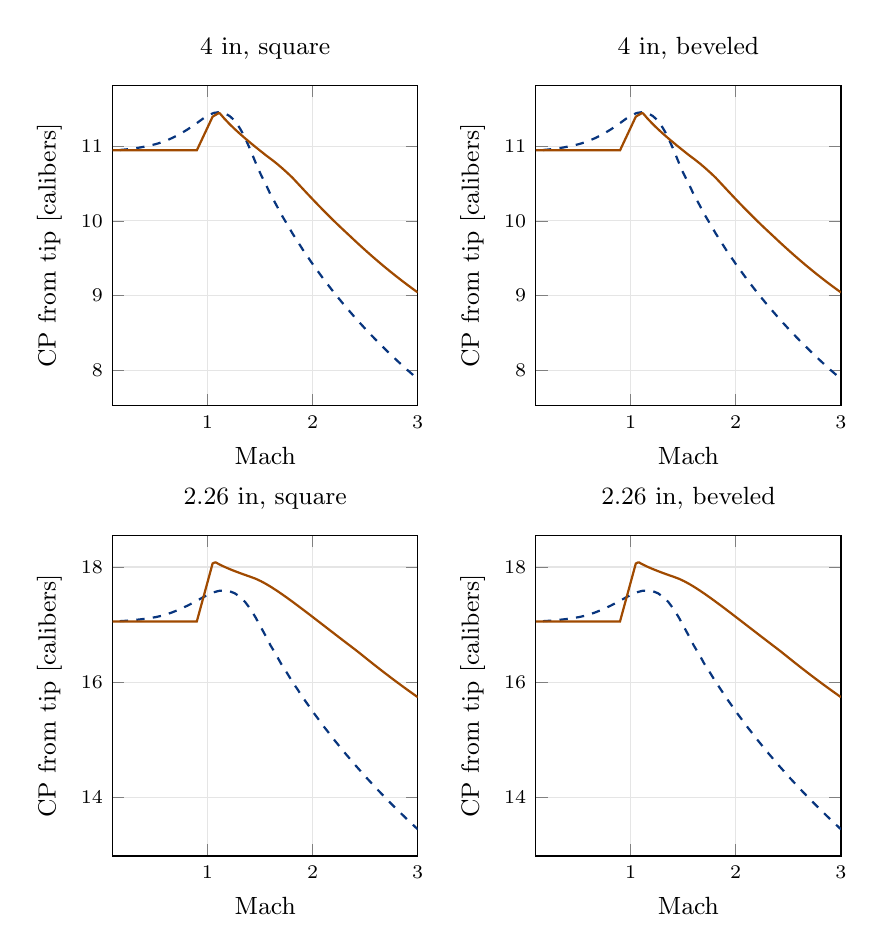
\begin{tikzpicture}
\begin{groupplot}[group style={group size=2 by 2,horizontal sep=1.50cm,vertical sep=1.65cm},width=.45\textwidth,height=5.65cm,grid=major,grid style={gray!20},tick label style={font=\scriptsize},label style={font=\small},title style={font=\small},scaled y ticks=false,yticklabel style={/pgf/number format/fixed,/pgf/number format/precision=3},unbounded coords=jump]
\nextgroupplot[title={4 in, square},xlabel={Mach},ylabel={CP from tip [calibers]},xmin=0.1,xmax=3]
\addplot[thick,B,dashed] coordinates {(0.01,10.93985) (0.06,10.94099) (0.11,10.94376) (0.16,10.94817) (0.21,10.95425) (0.26,10.96202) (0.31,10.97153) (0.36,10.98281) (0.41,10.99593) (0.46,11.01096) (0.51,11.02804) (0.56,11.04936) (0.61,11.07558) (0.66,11.1063) (0.71,11.1412) (0.76,11.18005) (0.81,11.2227) (0.86,11.26912) (0.91,11.31935) (0.96,11.37048) (1.01,11.41467) (1.06,11.44516) (1.11,11.45662) (1.16,11.44478) (1.21,11.40611) (1.24,11.36881) (1.26,11.33776) (1.29,11.28168) (1.31,11.2379) (1.33,11.18907) (1.36,11.10675) (1.41,10.94876) (1.46,10.77631) (1.49,10.67577) (1.51,10.61761) (1.56,10.47654) (1.6,10.35483) (1.61,10.33018) (1.66,10.20168) (1.7,10.09221) (1.71,10.06938) (1.76,9.951103) (1.81,9.830038) (1.86,9.720396) (1.91,9.608667) (1.96,9.506487) (2.01,9.402704) (2.06,9.30697) (2.11,9.209874) (2.16,9.119701) (2.21,9.028425) (2.26,8.943198) (2.31,8.857067) (2.36,8.776279) (2.41,8.694743) (2.46,8.617969) (2.51,8.540573) (2.56,8.46745) (2.61,8.393809) (2.66,8.32403) (2.71,8.253815) (2.76,8.18711) (2.81,8.120039) (2.86,8.056173) (2.91,7.991999) (2.96,7.930766) (3,7.880898)};
\addplot[thick,burntorange] coordinates {(0.01,10.94443) (0.06,10.94443) (0.11,10.94443) (0.16,10.94443) (0.21,10.94443) (0.26,10.94443) (0.31,10.94443) (0.36,10.94443) (0.41,10.94443) (0.46,10.94443) (0.51,10.94443) (0.56,10.94443) (0.61,10.94443) (0.66,10.94443) (0.71,10.94443) (0.76,10.94443) (0.81,10.94443) (0.86,10.94443) (0.9,10.94443) (0.91,10.97447) (0.96,11.12465) (1.01,11.27483) (1.05,11.39497) (1.06,11.40446) (1.11,11.44474) (1.12,11.43856) (1.16,11.37263) (1.21,11.29842) (1.26,11.23011) (1.31,11.1658) (1.36,11.10436) (1.41,11.04504) (1.46,10.9873) (1.51,10.93078) (1.56,10.87518) (1.61,10.82245) (1.66,10.76713) (1.71,10.70696) (1.76,10.64365) (1.81,10.57697) (1.86,10.50122) (1.91,10.42555) (1.96,10.35038) (2.01,10.27602) (2.06,10.20271) (2.11,10.13062) (2.16,10.05988) (2.21,9.990596) (2.26,9.92284) (2.31,9.856664) (2.36,9.791028) (2.41,9.724882) (2.46,9.659958) (2.51,9.596287) (2.56,9.533895) (2.61,9.472797) (2.66,9.413013) (2.71,9.354546) (2.76,9.297407) (2.81,9.241598) (2.86,9.187121) (2.91,9.133971) (2.96,9.082146) (3,9.041639)};
\nextgroupplot[title={4 in, beveled},xlabel={Mach},ylabel={CP from tip [calibers]},xmin=0.1,xmax=3]
\addplot[thick,B,dashed] coordinates {(0.01,10.93985) (0.06,10.94099) (0.11,10.94376) (0.16,10.94817) (0.21,10.95425) (0.26,10.96202) (0.31,10.97153) (0.36,10.98281) (0.41,10.99593) (0.46,11.01096) (0.51,11.02804) (0.56,11.04936) (0.61,11.07558) (0.66,11.1063) (0.71,11.1412) (0.76,11.18005) (0.81,11.2227) (0.86,11.26912) (0.91,11.31935) (0.96,11.37048) (1.01,11.41467) (1.06,11.44516) (1.11,11.45662) (1.16,11.44478) (1.21,11.40611) (1.24,11.36881) (1.26,11.33776) (1.29,11.28168) (1.31,11.2379) (1.33,11.18907) (1.36,11.10675) (1.41,10.94876) (1.46,10.77631) (1.49,10.67577) (1.51,10.61761) (1.56,10.47654) (1.6,10.35483) (1.61,10.33018) (1.66,10.20168) (1.7,10.09221) (1.71,10.06938) (1.76,9.951103) (1.81,9.830038) (1.86,9.720396) (1.91,9.608667) (1.96,9.506487) (2.01,9.402704) (2.06,9.30697) (2.11,9.209874) (2.16,9.119701) (2.21,9.028425) (2.26,8.943198) (2.31,8.857067) (2.36,8.776279) (2.41,8.694743) (2.46,8.617969) (2.51,8.540573) (2.56,8.46745) (2.61,8.393809) (2.66,8.32403) (2.71,8.253815) (2.76,8.18711) (2.81,8.120039) (2.86,8.056173) (2.91,7.991999) (2.96,7.930766) (3,7.880898)};
\addplot[thick,burntorange] coordinates {(0.01,10.94443) (0.06,10.94443) (0.11,10.94443) (0.16,10.94443) (0.21,10.94443) (0.26,10.94443) (0.31,10.94443) (0.36,10.94443) (0.41,10.94443) (0.46,10.94443) (0.51,10.94443) (0.56,10.94443) (0.61,10.94443) (0.66,10.94443) (0.71,10.94443) (0.76,10.94443) (0.81,10.94443) (0.86,10.94443) (0.9,10.94443) (0.91,10.97447) (0.96,11.12465) (1.01,11.27483) (1.05,11.39497) (1.06,11.40446) (1.11,11.44474) (1.12,11.43856) (1.16,11.37263) (1.21,11.29842) (1.26,11.23011) (1.31,11.1658) (1.36,11.10436) (1.41,11.04504) (1.46,10.9873) (1.51,10.93078) (1.56,10.87518) (1.61,10.82245) (1.66,10.76713) (1.71,10.70696) (1.76,10.64365) (1.81,10.57697) (1.86,10.50122) (1.91,10.42555) (1.96,10.35038) (2.01,10.27602) (2.06,10.20271) (2.11,10.13062) (2.16,10.05988) (2.21,9.990596) (2.26,9.92284) (2.31,9.856664) (2.36,9.791028) (2.41,9.724882) (2.46,9.659958) (2.51,9.596287) (2.56,9.533895) (2.61,9.472797) (2.66,9.413013) (2.71,9.354546) (2.76,9.297407) (2.81,9.241598) (2.86,9.187121) (2.91,9.133971) (2.96,9.082146) (3,9.041639)};
\nextgroupplot[title={2.26 in, square},xlabel={Mach},ylabel={CP from tip [calibers]},xmin=0.1,xmax=3]
\addplot[thick,B,dashed] coordinates {(0.01,17.05047) (0.06,17.05151) (0.11,17.05403) (0.16,17.05804) (0.21,17.06355) (0.26,17.07059) (0.31,17.07918) (0.36,17.08935) (0.41,17.10114) (0.46,17.11459) (0.51,17.12986) (0.56,17.15016) (0.61,17.1764) (0.66,17.20783) (0.71,17.24381) (0.76,17.28378) (0.81,17.3273) (0.86,17.37402) (0.91,17.42368) (0.96,17.47466) (1.01,17.52189) (1.06,17.5603) (1.11,17.58545) (1.16,17.59345) (1.21,17.58083) (1.26,17.54452) (1.31,17.4818) (1.36,17.39048) (1.41,17.26946) (1.46,17.11972) (1.51,16.95091) (1.56,16.7844) (1.6,16.63935) (1.61,16.60989) (1.66,16.45543) (1.7,16.32276) (1.71,16.295) (1.76,16.15052) (1.81,16.00147) (1.86,15.86559) (1.91,15.72615) (1.96,15.59785) (2.01,15.4667) (2.06,15.34499) (2.11,15.22074) (2.16,15.10467) (2.21,14.98647) (2.26,14.8755) (2.31,14.76271) (2.36,14.65637) (2.41,14.54847) (2.46,14.44637) (2.51,14.34292) (2.56,14.24473) (2.61,14.14537) (2.66,14.0508) (2.71,13.9552) (2.76,13.86399) (2.81,13.77189) (2.86,13.68382) (2.91,13.59497) (2.96,13.50985) (3,13.44028)};
\addplot[thick,burntorange] coordinates {(0.01,17.05341) (0.06,17.05341) (0.11,17.05341) (0.16,17.05341) (0.21,17.05341) (0.26,17.05341) (0.31,17.05341) (0.36,17.05341) (0.41,17.05341) (0.46,17.05341) (0.51,17.05341) (0.56,17.05341) (0.61,17.05341) (0.66,17.05341) (0.71,17.05341) (0.76,17.05341) (0.81,17.05341) (0.86,17.05341) (0.9,17.05341) (0.91,17.12056) (0.96,17.45628) (1.01,17.79201) (1.05,18.06058) (1.06,18.06975) (1.07,18.07831) (1.08,18.08077) (1.11,18.05012) (1.16,18.00566) (1.21,17.96607) (1.26,17.92951) (1.31,17.895) (1.36,17.86196) (1.41,17.83) (1.46,17.79603) (1.51,17.75337) (1.56,17.70373) (1.61,17.64872) (1.66,17.58959) (1.71,17.52731) (1.76,17.46262) (1.81,17.3961) (1.86,17.32821) (1.91,17.25931) (1.96,17.18969) (2.01,17.11957) (2.06,17.04915) (2.11,16.97859) (2.16,16.908) (2.21,16.83751) (2.26,16.76719) (2.31,16.69714) (2.36,16.6274) (2.41,16.55805) (2.46,16.4856) (2.51,16.41192) (2.56,16.33907) (2.61,16.26707) (2.66,16.19596) (2.71,16.12577) (2.76,16.05652) (2.81,15.98823) (2.86,15.92092) (2.91,15.85461) (2.96,15.7893) (3,15.73779)};
\nextgroupplot[title={2.26 in, beveled},xlabel={Mach},ylabel={CP from tip [calibers]},xmin=0.1,xmax=3]
\addplot[thick,B,dashed] coordinates {(0.01,17.05047) (0.06,17.05151) (0.11,17.05403) (0.16,17.05804) (0.21,17.06355) (0.26,17.07059) (0.31,17.07918) (0.36,17.08935) (0.41,17.10114) (0.46,17.11459) (0.51,17.12986) (0.56,17.15016) (0.61,17.1764) (0.66,17.20783) (0.71,17.24381) (0.76,17.28378) (0.81,17.3273) (0.86,17.37402) (0.91,17.42368) (0.96,17.47466) (1.01,17.52189) (1.06,17.5603) (1.11,17.58545) (1.16,17.59345) (1.21,17.58083) (1.26,17.54452) (1.31,17.4818) (1.36,17.39048) (1.41,17.26946) (1.46,17.11972) (1.51,16.95091) (1.56,16.7844) (1.6,16.63935) (1.61,16.60989) (1.66,16.45543) (1.7,16.32276) (1.71,16.295) (1.76,16.15052) (1.81,16.00147) (1.86,15.86559) (1.91,15.72615) (1.96,15.59785) (2.01,15.4667) (2.06,15.34499) (2.11,15.22074) (2.16,15.10467) (2.21,14.98647) (2.26,14.8755) (2.31,14.76271) (2.36,14.65637) (2.41,14.54847) (2.46,14.44637) (2.51,14.34292) (2.56,14.24473) (2.61,14.14537) (2.66,14.0508) (2.71,13.9552) (2.76,13.86399) (2.81,13.77189) (2.86,13.68382) (2.91,13.59497) (2.96,13.50985) (3,13.44028)};
\addplot[thick,burntorange] coordinates {(0.01,17.05341) (0.06,17.05341) (0.11,17.05341) (0.16,17.05341) (0.21,17.05341) (0.26,17.05341) (0.31,17.05341) (0.36,17.05341) (0.41,17.05341) (0.46,17.05341) (0.51,17.05341) (0.56,17.05341) (0.61,17.05341) (0.66,17.05341) (0.71,17.05341) (0.76,17.05341) (0.81,17.05341) (0.86,17.05341) (0.9,17.05341) (0.91,17.12056) (0.96,17.45628) (1.01,17.79201) (1.05,18.06058) (1.06,18.06975) (1.07,18.07831) (1.08,18.08077) (1.11,18.05012) (1.16,18.00566) (1.21,17.96607) (1.26,17.92951) (1.31,17.895) (1.36,17.86196) (1.41,17.83) (1.46,17.79603) (1.51,17.75337) (1.56,17.70373) (1.61,17.64872) (1.66,17.58959) (1.71,17.52731) (1.76,17.46262) (1.81,17.3961) (1.86,17.32821) (1.91,17.25931) (1.96,17.18969) (2.01,17.11957) (2.06,17.04915) (2.11,16.97859) (2.16,16.908) (2.21,16.83751) (2.26,16.76719) (2.31,16.69714) (2.36,16.6274) (2.41,16.55805) (2.46,16.4856) (2.51,16.41192) (2.56,16.33907) (2.61,16.26707) (2.66,16.19596) (2.71,16.12577) (2.76,16.05652) (2.81,15.98823) (2.86,15.92092) (2.91,15.85461) (2.96,15.7893) (3,15.73779)};
\end{groupplot}\end{tikzpicture}
\caption{CP is measured from the nose tip in body diameters; this is not a stability margin. OR warns of limitations of its body-force treatment above Mach 1.1.}\label{fig:atlas-24-cp-0}
\end{figure}
\noindent{\footnotesize Export files: \code{24-cp-0.svg} and \code{24-cp-0.png}.\\ Directory: \code{aerodynamic-investigation/extended/figures/}.}

\clearpage\subsubsection*{Center of pressure at 4 degrees}
\begin{figure}[H]\centering
{\footnotesize\begin{tabular}{ll}
\tikz[baseline=-.5ex]{\draw[thick,B,dashed] (0,0)--(.40,0);}\ MIT OR & \tikz[baseline=-.5ex]{\draw[thick,burntorange] (0,0)--(.40,0);}\ RASAero\\
\end{tabular}}\par\vspace{.7em}
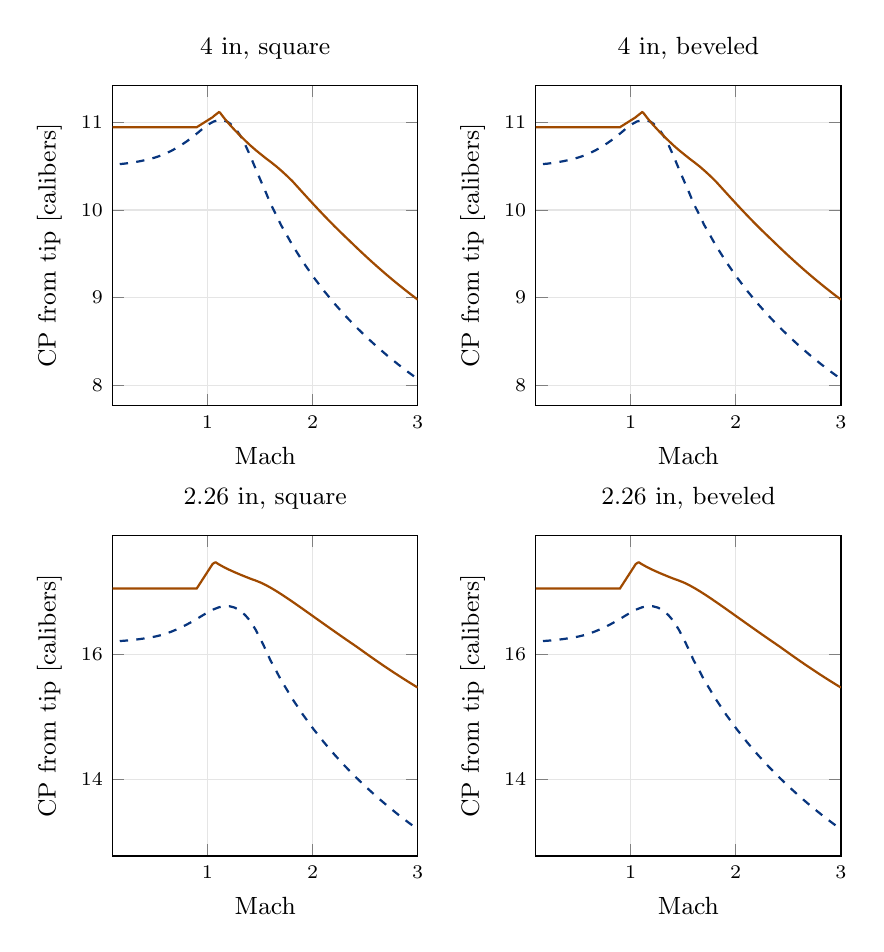
\begin{tikzpicture}
\begin{groupplot}[group style={group size=2 by 2,horizontal sep=1.50cm,vertical sep=1.65cm},width=.45\textwidth,height=5.65cm,grid=major,grid style={gray!20},tick label style={font=\scriptsize},label style={font=\small},title style={font=\small},scaled y ticks=false,yticklabel style={/pgf/number format/fixed,/pgf/number format/precision=3},unbounded coords=jump]
\nextgroupplot[title={4 in, square},xlabel={Mach},ylabel={CP from tip [calibers]},xmin=0.1,xmax=3]
\addplot[thick,B,dashed] coordinates {(0.01,10.5144) (0.06,10.51551) (0.11,10.51821) (0.16,10.5225) (0.21,10.52842) (0.26,10.536) (0.31,10.54526) (0.36,10.55628) (0.41,10.5691) (0.46,10.5838) (0.51,10.60054) (0.56,10.6212) (0.61,10.64639) (0.66,10.6758) (0.71,10.70919) (0.76,10.74643) (0.81,10.78745) (0.86,10.83228) (0.91,10.88106) (0.96,10.93126) (1.01,10.97589) (1.06,11.00873) (1.11,11.02477) (1.12,11.02559) (1.16,11.01999) (1.19,11.00578) (1.21,10.99124) (1.24,10.96147) (1.26,10.93619) (1.28,10.9065) (1.31,10.85367) (1.33,10.81303) (1.36,10.74436) (1.41,10.6123) (1.46,10.46726) (1.51,10.32772) (1.56,10.19009) (1.6,10.07221) (1.61,10.04922) (1.66,9.930043) (1.7,9.829356) (1.71,9.808874) (1.76,9.703352) (1.81,9.596574) (1.86,9.501802) (1.91,9.406233) (1.96,9.320257) (2.01,9.233773) (2.06,9.155104) (2.11,9.076029) (2.16,9.003484) (2.21,8.930664) (2.26,8.863406) (2.31,8.795967) (2.36,8.733331) (2.41,8.670583) (2.46,8.612029) (2.51,8.553412) (2.56,8.498494) (2.61,8.44355) (2.66,8.391893) (2.71,8.340239) (2.76,8.291525) (2.81,8.242836) (2.86,8.196793) (2.91,8.150791) (2.96,8.107184) (3,8.071837)};
\addplot[thick,burntorange] coordinates {(0.01,10.94443) (0.06,10.94443) (0.11,10.94443) (0.16,10.94443) (0.21,10.94443) (0.26,10.94443) (0.31,10.94443) (0.36,10.94443) (0.41,10.94443) (0.46,10.94443) (0.51,10.94443) (0.56,10.94443) (0.61,10.94443) (0.66,10.94443) (0.71,10.94443) (0.76,10.94443) (0.81,10.94443) (0.86,10.94443) (0.9,10.94443) (0.91,10.95199) (0.96,10.98978) (1.01,11.02758) (1.05,11.05781) (1.06,11.06903) (1.11,11.11606) (1.12,11.11081) (1.16,11.04772) (1.21,10.97676) (1.26,10.91149) (1.31,10.85009) (1.36,10.79148) (1.41,10.73493) (1.46,10.68265) (1.51,10.6339) (1.56,10.586) (1.61,10.54086) (1.66,10.49317) (1.71,10.44079) (1.76,10.38537) (1.81,10.32689) (1.86,10.26066) (1.91,10.19444) (1.96,10.12863) (2.01,10.06352) (2.06,9.999335) (2.11,9.936226) (2.16,9.87431) (2.21,9.813674) (2.26,9.754379) (2.31,9.696467) (2.36,9.639028) (2.41,9.58106) (2.46,9.524123) (2.51,9.468236) (2.56,9.413416) (2.61,9.359669) (2.66,9.307009) (2.71,9.255433) (2.76,9.204946) (2.81,9.155547) (2.86,9.107232) (2.91,9.059999) (2.96,9.013842) (3,8.977689)};
\nextgroupplot[title={4 in, beveled},xlabel={Mach},ylabel={CP from tip [calibers]},xmin=0.1,xmax=3]
\addplot[thick,B,dashed] coordinates {(0.01,10.5144) (0.06,10.51551) (0.11,10.51821) (0.16,10.5225) (0.21,10.52842) (0.26,10.536) (0.31,10.54526) (0.36,10.55628) (0.41,10.5691) (0.46,10.5838) (0.51,10.60054) (0.56,10.6212) (0.61,10.64639) (0.66,10.6758) (0.71,10.70919) (0.76,10.74643) (0.81,10.78745) (0.86,10.83228) (0.91,10.88106) (0.96,10.93126) (1.01,10.97589) (1.06,11.00873) (1.11,11.02477) (1.12,11.02559) (1.16,11.01999) (1.19,11.00578) (1.21,10.99124) (1.24,10.96147) (1.26,10.93619) (1.28,10.9065) (1.31,10.85367) (1.33,10.81303) (1.36,10.74436) (1.41,10.6123) (1.46,10.46726) (1.51,10.32772) (1.56,10.19009) (1.6,10.07221) (1.61,10.04922) (1.66,9.930043) (1.7,9.829356) (1.71,9.808874) (1.76,9.703352) (1.81,9.596574) (1.86,9.501802) (1.91,9.406233) (1.96,9.320257) (2.01,9.233773) (2.06,9.155104) (2.11,9.076029) (2.16,9.003484) (2.21,8.930664) (2.26,8.863406) (2.31,8.795967) (2.36,8.733331) (2.41,8.670583) (2.46,8.612029) (2.51,8.553412) (2.56,8.498494) (2.61,8.44355) (2.66,8.391893) (2.71,8.340239) (2.76,8.291525) (2.81,8.242836) (2.86,8.196793) (2.91,8.150791) (2.96,8.107184) (3,8.071837)};
\addplot[thick,burntorange] coordinates {(0.01,10.94443) (0.06,10.94443) (0.11,10.94443) (0.16,10.94443) (0.21,10.94443) (0.26,10.94443) (0.31,10.94443) (0.36,10.94443) (0.41,10.94443) (0.46,10.94443) (0.51,10.94443) (0.56,10.94443) (0.61,10.94443) (0.66,10.94443) (0.71,10.94443) (0.76,10.94443) (0.81,10.94443) (0.86,10.94443) (0.9,10.94443) (0.91,10.95199) (0.96,10.98978) (1.01,11.02758) (1.05,11.05781) (1.06,11.06903) (1.11,11.11606) (1.12,11.11081) (1.16,11.04772) (1.21,10.97676) (1.26,10.91149) (1.31,10.85009) (1.36,10.79148) (1.41,10.73493) (1.46,10.68265) (1.51,10.6339) (1.56,10.586) (1.61,10.54086) (1.66,10.49317) (1.71,10.44079) (1.76,10.38537) (1.81,10.32689) (1.86,10.26066) (1.91,10.19444) (1.96,10.12863) (2.01,10.06352) (2.06,9.999335) (2.11,9.936226) (2.16,9.87431) (2.21,9.813674) (2.26,9.754379) (2.31,9.696467) (2.36,9.639028) (2.41,9.58106) (2.46,9.524123) (2.51,9.468236) (2.56,9.413416) (2.61,9.359669) (2.66,9.307009) (2.71,9.255433) (2.76,9.204946) (2.81,9.155547) (2.86,9.107232) (2.91,9.059999) (2.96,9.013842) (3,8.977689)};
\nextgroupplot[title={2.26 in, square},xlabel={Mach},ylabel={CP from tip [calibers]},xmin=0.1,xmax=3]
\addplot[thick,B,dashed] coordinates {(0.01,16.20243) (0.06,16.20351) (0.11,16.20613) (0.16,16.21031) (0.21,16.21606) (0.26,16.2234) (0.31,16.23236) (0.36,16.24298) (0.41,16.25531) (0.46,16.26938) (0.51,16.28537) (0.56,16.30598) (0.61,16.33203) (0.66,16.3629) (0.71,16.39811) (0.76,16.43723) (0.81,16.47993) (0.86,16.52599) (0.91,16.57526) (0.96,16.62659) (1.01,16.67596) (1.06,16.71893) (1.11,16.75123) (1.16,16.76892) (1.18,16.77109) (1.21,16.76838) (1.26,16.74627) (1.31,16.69961) (1.36,16.62578) (1.39,16.56758) (1.41,16.52281) (1.43,16.47321) (1.46,16.38983) (1.51,16.22912) (1.56,16.0534) (1.6,15.90188) (1.61,15.87227) (1.66,15.71817) (1.7,15.58722) (1.71,15.56054) (1.76,15.42259) (1.8,15.30659) (1.81,15.28227) (1.86,15.15719) (1.91,15.03048) (1.96,14.91606) (2.01,14.80048) (2.06,14.69496) (2.11,14.58845) (2.16,14.49038) (2.21,14.39158) (2.26,14.30001) (2.31,14.20789) (2.36,14.12206) (2.41,14.03581) (2.46,13.95509) (2.51,13.87405) (2.56,13.79792) (2.61,13.72155) (2.66,13.64956) (2.71,13.57739) (2.76,13.50918) (2.81,13.44083) (2.86,13.37605) (2.91,13.31118) (2.96,13.24956) (3,13.19952)};
\addplot[thick,burntorange] coordinates {(0.01,17.05341) (0.06,17.05341) (0.11,17.05341) (0.16,17.05341) (0.21,17.05341) (0.26,17.05341) (0.31,17.05341) (0.36,17.05341) (0.41,17.05341) (0.46,17.05341) (0.51,17.05341) (0.56,17.05341) (0.61,17.05341) (0.66,17.05341) (0.71,17.05341) (0.76,17.05341) (0.81,17.05341) (0.86,17.05341) (0.9,17.05341) (0.91,17.07944) (0.96,17.20958) (1.01,17.33973) (1.05,17.44384) (1.06,17.45523) (1.07,17.46581) (1.08,17.46946) (1.11,17.43755) (1.16,17.39124) (1.21,17.35001) (1.26,17.31193) (1.31,17.276) (1.36,17.24159) (1.41,17.20832) (1.46,17.17843) (1.51,17.14435) (1.56,17.10313) (1.61,17.05652) (1.66,17.0059) (1.71,16.95229) (1.76,16.89651) (1.81,16.83916) (1.86,16.78072) (1.91,16.72155) (1.96,16.66193) (2.01,16.6021) (2.06,16.54223) (2.11,16.48248) (2.16,16.42294) (2.21,16.36372) (2.26,16.30488) (2.31,16.2465) (2.36,16.18861) (2.41,16.13126) (2.46,16.0716) (2.51,16.01113) (2.56,15.95153) (2.61,15.89283) (2.66,15.83503) (2.71,15.77815) (2.76,15.7222) (2.81,15.66718) (2.86,15.61311) (2.91,15.55998) (2.96,15.5078) (3,15.46674)};
\nextgroupplot[title={2.26 in, beveled},xlabel={Mach},ylabel={CP from tip [calibers]},xmin=0.1,xmax=3]
\addplot[thick,B,dashed] coordinates {(0.01,16.20243) (0.06,16.20351) (0.11,16.20613) (0.16,16.21031) (0.21,16.21606) (0.26,16.2234) (0.31,16.23236) (0.36,16.24298) (0.41,16.25531) (0.46,16.26938) (0.51,16.28537) (0.56,16.30598) (0.61,16.33203) (0.66,16.3629) (0.71,16.39811) (0.76,16.43723) (0.81,16.47993) (0.86,16.52599) (0.91,16.57526) (0.96,16.62659) (1.01,16.67596) (1.06,16.71893) (1.11,16.75123) (1.16,16.76892) (1.18,16.77109) (1.21,16.76838) (1.26,16.74627) (1.31,16.69961) (1.36,16.62578) (1.39,16.56758) (1.41,16.52281) (1.43,16.47321) (1.46,16.38983) (1.51,16.22912) (1.56,16.0534) (1.6,15.90188) (1.61,15.87227) (1.66,15.71817) (1.7,15.58722) (1.71,15.56054) (1.76,15.42259) (1.8,15.30659) (1.81,15.28227) (1.86,15.15719) (1.91,15.03048) (1.96,14.91606) (2.01,14.80048) (2.06,14.69496) (2.11,14.58845) (2.16,14.49038) (2.21,14.39158) (2.26,14.30001) (2.31,14.20789) (2.36,14.12206) (2.41,14.03581) (2.46,13.95509) (2.51,13.87405) (2.56,13.79792) (2.61,13.72155) (2.66,13.64956) (2.71,13.57739) (2.76,13.50918) (2.81,13.44083) (2.86,13.37605) (2.91,13.31118) (2.96,13.24956) (3,13.19952)};
\addplot[thick,burntorange] coordinates {(0.01,17.05341) (0.06,17.05341) (0.11,17.05341) (0.16,17.05341) (0.21,17.05341) (0.26,17.05341) (0.31,17.05341) (0.36,17.05341) (0.41,17.05341) (0.46,17.05341) (0.51,17.05341) (0.56,17.05341) (0.61,17.05341) (0.66,17.05341) (0.71,17.05341) (0.76,17.05341) (0.81,17.05341) (0.86,17.05341) (0.9,17.05341) (0.91,17.07944) (0.96,17.20958) (1.01,17.33973) (1.05,17.44384) (1.06,17.45523) (1.07,17.46581) (1.08,17.46946) (1.11,17.43755) (1.16,17.39124) (1.21,17.35001) (1.26,17.31193) (1.31,17.276) (1.36,17.24159) (1.41,17.20832) (1.46,17.17843) (1.51,17.14435) (1.56,17.10313) (1.61,17.05652) (1.66,17.0059) (1.71,16.95229) (1.76,16.89651) (1.81,16.83916) (1.86,16.78072) (1.91,16.72155) (1.96,16.66193) (2.01,16.6021) (2.06,16.54223) (2.11,16.48248) (2.16,16.42294) (2.21,16.36372) (2.26,16.30488) (2.31,16.2465) (2.36,16.18861) (2.41,16.13126) (2.46,16.0716) (2.51,16.01113) (2.56,15.95153) (2.61,15.89283) (2.66,15.83503) (2.71,15.77815) (2.76,15.7222) (2.81,15.66718) (2.86,15.61311) (2.91,15.55998) (2.96,15.5078) (3,15.46674)};
\end{groupplot}\end{tikzpicture}
\caption{CP is measured from the nose tip in body diameters; this is not a stability margin. OR warns of limitations of its body-force treatment above Mach 1.1.}\label{fig:atlas-24-cp-4}
\end{figure}
\noindent{\footnotesize Export files: \code{24-cp-4.svg} and \code{24-cp-4.png}.\\ Directory: \code{aerodynamic-investigation/extended/figures/}.}

\clearpage\subsubsection*{Normal-force slope over 0 to 4 degrees}
\begin{figure}[H]\centering
{\footnotesize\begin{tabular}{ll}
\tikz[baseline=-.5ex]{\draw[thick,B,dashed] (0,0)--(.40,0);}\ MIT OR & \tikz[baseline=-.5ex]{\draw[thick,burntorange] (0,0)--(.40,0);}\ RASAero\\
\end{tabular}}\par\vspace{.7em}
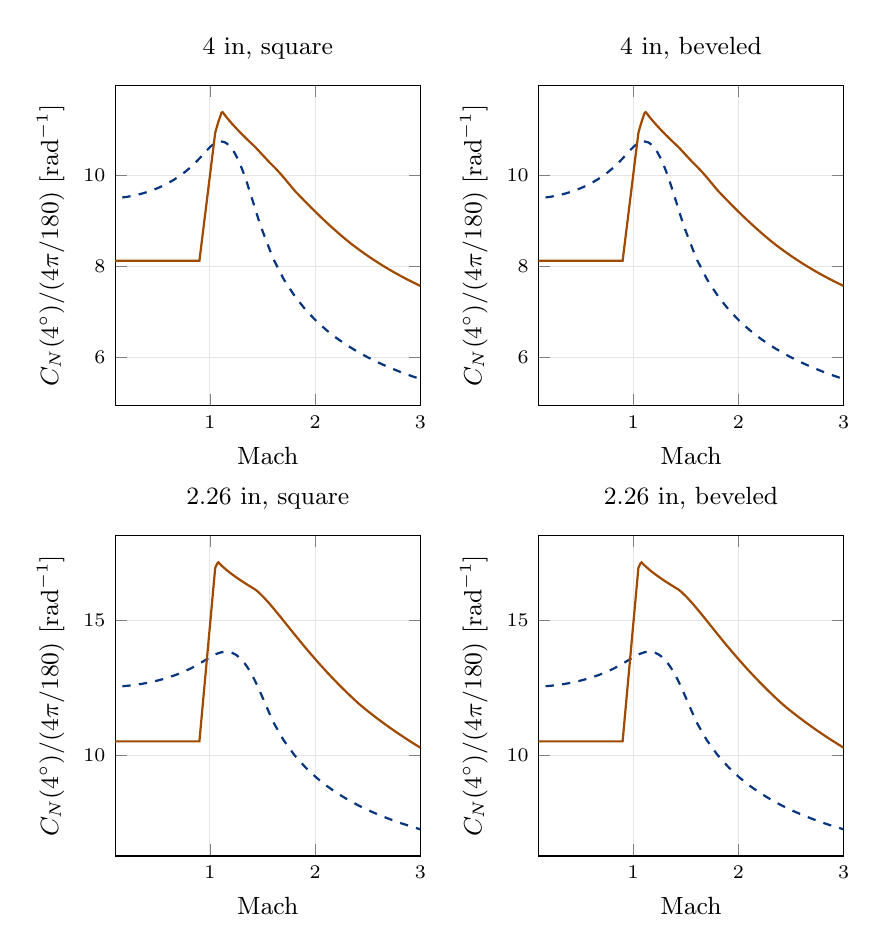
\begin{tikzpicture}
\begin{groupplot}[group style={group size=2 by 2,horizontal sep=1.50cm,vertical sep=1.65cm},width=.45\textwidth,height=5.65cm,grid=major,grid style={gray!20},tick label style={font=\scriptsize},label style={font=\small},title style={font=\small},scaled y ticks=false,yticklabel style={/pgf/number format/fixed,/pgf/number format/precision=3},unbounded coords=jump]
\nextgroupplot[title={4 in, square},xlabel={Mach},ylabel={$C_N(4^\circ)/(4\pi/180)$ [rad$^{-1}$]},xmin=0.1,xmax=3]
\addplot[thick,B,dashed] coordinates {(0.01,9.489541) (0.06,9.492507) (0.11,9.49973) (0.16,9.511269) (0.21,9.527213) (0.26,9.547691) (0.31,9.572871) (0.36,9.602966) (0.41,9.638237) (0.46,9.679007) (0.51,9.725662) (0.56,9.77867) (0.61,9.838595) (0.66,9.906119) (0.71,9.982068) (0.76,10.06745) (0.81,10.16353) (0.86,10.27184) (0.91,10.39428) (0.96,10.5242) (1.01,10.63937) (1.04,10.69232) (1.06,10.71828) (1.1,10.74299) (1.11,10.74282) (1.14,10.72553) (1.16,10.69929) (1.19,10.63679) (1.21,10.57939) (1.23,10.50938) (1.26,10.38118) (1.28,10.28092) (1.31,10.11009) (1.33,9.984013) (1.36,9.779838) (1.41,9.413495) (1.46,9.044407) (1.49,8.8397) (1.51,8.716843) (1.56,8.417353) (1.6,8.177761) (1.61,8.132521) (1.66,7.906321) (1.7,7.725362) (1.71,7.689512) (1.76,7.510266) (1.81,7.33751) (1.86,7.190719) (1.91,7.048658) (1.96,6.925519) (2.01,6.805963) (2.06,6.700743) (2.11,6.598321) (2.16,6.50709) (2.21,6.418097) (2.26,6.338049) (2.31,6.259825) (2.36,6.188892) (2.41,6.119469) (2.46,6.056085) (2.51,5.993969) (2.56,5.936923) (2.61,5.880953) (2.66,5.82929) (2.71,5.778551) (2.76,5.731507) (2.81,5.685262) (2.86,5.642216) (2.91,5.599868) (2.96,5.560309) (3,5.528662)};
\addplot[thick,burntorange] coordinates {(0.01,8.123345) (0.06,8.123345) (0.11,8.123345) (0.16,8.123345) (0.21,8.123345) (0.26,8.123345) (0.31,8.123345) (0.36,8.123345) (0.41,8.123345) (0.46,8.123345) (0.51,8.123345) (0.56,8.123345) (0.61,8.123345) (0.66,8.123345) (0.71,8.123345) (0.76,8.123345) (0.81,8.123345) (0.86,8.123345) (0.9,8.123345) (0.91,8.31043) (0.96,9.245857) (1.01,10.18128) (1.05,10.92962) (1.06,11.01667) (1.08,11.17228) (1.11,11.37514) (1.12,11.38686) (1.16,11.26745) (1.21,11.13211) (1.26,11.0068) (1.31,10.88831) (1.36,10.77474) (1.41,10.66483) (1.43,10.62169) (1.46,10.54722) (1.51,10.42243) (1.56,10.29937) (1.61,10.18363) (1.66,10.06165) (1.71,9.928472) (1.76,9.789285) (1.81,9.65081) (1.86,9.53155) (1.91,9.413077) (1.96,9.296365) (2.01,9.182024) (2.06,9.070435) (2.11,8.961806) (2.16,8.856236) (2.21,8.753745) (2.26,8.654296) (2.31,8.557822) (2.36,8.466975) (2.41,8.380359) (2.46,8.297032) (2.51,8.216863) (2.56,8.139725) (2.61,8.065484) (2.66,7.994017) (2.71,7.925197) (2.76,7.858909) (2.81,7.795037) (2.86,7.733474) (2.91,7.674113) (2.96,7.616858) (3,7.572505)};
\nextgroupplot[title={4 in, beveled},xlabel={Mach},ylabel={$C_N(4^\circ)/(4\pi/180)$ [rad$^{-1}$]},xmin=0.1,xmax=3]
\addplot[thick,B,dashed] coordinates {(0.01,9.489541) (0.06,9.492507) (0.11,9.49973) (0.16,9.511269) (0.21,9.527213) (0.26,9.547691) (0.31,9.572871) (0.36,9.602966) (0.41,9.638237) (0.46,9.679007) (0.51,9.725662) (0.56,9.77867) (0.61,9.838595) (0.66,9.906119) (0.71,9.982068) (0.76,10.06745) (0.81,10.16353) (0.86,10.27184) (0.91,10.39428) (0.96,10.5242) (1.01,10.63937) (1.04,10.69232) (1.06,10.71828) (1.1,10.74299) (1.11,10.74282) (1.14,10.72553) (1.16,10.69929) (1.19,10.63679) (1.21,10.57939) (1.23,10.50938) (1.26,10.38118) (1.28,10.28092) (1.31,10.11009) (1.33,9.984013) (1.36,9.779838) (1.41,9.413495) (1.46,9.044407) (1.49,8.8397) (1.51,8.716843) (1.56,8.417353) (1.6,8.177761) (1.61,8.132521) (1.66,7.906321) (1.7,7.725362) (1.71,7.689512) (1.76,7.510266) (1.81,7.33751) (1.86,7.190719) (1.91,7.048658) (1.96,6.925519) (2.01,6.805963) (2.06,6.700743) (2.11,6.598321) (2.16,6.50709) (2.21,6.418097) (2.26,6.338049) (2.31,6.259825) (2.36,6.188892) (2.41,6.119469) (2.46,6.056085) (2.51,5.993969) (2.56,5.936923) (2.61,5.880953) (2.66,5.82929) (2.71,5.778551) (2.76,5.731507) (2.81,5.685262) (2.86,5.642216) (2.91,5.599868) (2.96,5.560309) (3,5.528662)};
\addplot[thick,burntorange] coordinates {(0.01,8.123345) (0.06,8.123345) (0.11,8.123345) (0.16,8.123345) (0.21,8.123345) (0.26,8.123345) (0.31,8.123345) (0.36,8.123345) (0.41,8.123345) (0.46,8.123345) (0.51,8.123345) (0.56,8.123345) (0.61,8.123345) (0.66,8.123345) (0.71,8.123345) (0.76,8.123345) (0.81,8.123345) (0.86,8.123345) (0.9,8.123345) (0.91,8.31043) (0.96,9.245857) (1.01,10.18128) (1.05,10.92962) (1.06,11.01667) (1.08,11.17228) (1.11,11.37514) (1.12,11.38686) (1.16,11.26745) (1.21,11.13211) (1.26,11.0068) (1.31,10.88831) (1.36,10.77474) (1.41,10.66483) (1.43,10.62169) (1.46,10.54722) (1.51,10.42243) (1.56,10.29937) (1.61,10.18363) (1.66,10.06165) (1.71,9.928472) (1.76,9.789285) (1.81,9.65081) (1.86,9.53155) (1.91,9.413077) (1.96,9.296365) (2.01,9.182024) (2.06,9.070435) (2.11,8.961806) (2.16,8.856236) (2.21,8.753745) (2.26,8.654296) (2.31,8.557822) (2.36,8.466975) (2.41,8.380359) (2.46,8.297032) (2.51,8.216863) (2.56,8.139725) (2.61,8.065484) (2.66,7.994017) (2.71,7.925197) (2.76,7.858909) (2.81,7.795037) (2.86,7.733474) (2.91,7.674113) (2.96,7.616858) (3,7.572505)};
\nextgroupplot[title={2.26 in, square},xlabel={Mach},ylabel={$C_N(4^\circ)/(4\pi/180)$ [rad$^{-1}$]},xmin=0.1,xmax=3]
\addplot[thick,B,dashed] coordinates {(0.01,12.52853) (0.06,12.53162) (0.11,12.53915) (0.16,12.55116) (0.21,12.56772) (0.26,12.58893) (0.31,12.61493) (0.36,12.64587) (0.41,12.68197) (0.46,12.72345) (0.51,12.77061) (0.56,12.82379) (0.61,12.88339) (0.66,12.94988) (0.71,13.02381) (0.76,13.10585) (0.81,13.19678) (0.86,13.29752) (0.91,13.40921) (0.96,13.52958) (1.01,13.6464) (1.06,13.74503) (1.11,13.81073) (1.15,13.83013) (1.16,13.82951) (1.19,13.81304) (1.21,13.78905) (1.24,13.73216) (1.26,13.67961) (1.29,13.57803) (1.31,13.49486) (1.33,13.39927) (1.36,13.23282) (1.38,13.10689) (1.41,12.89672) (1.43,12.74341) (1.46,12.4959) (1.51,12.04942) (1.56,11.59971) (1.6,11.23994) (1.61,11.17201) (1.66,10.83235) (1.7,10.56062) (1.71,10.50679) (1.76,10.23764) (1.8,10.02231) (1.81,9.978228) (1.86,9.757809) (1.91,9.544492) (1.96,9.359587) (2.01,9.180064) (2.06,9.022067) (2.11,8.868271) (2.16,8.73128) (2.21,8.597648) (2.26,8.47745) (2.31,8.359989) (2.36,8.253477) (2.41,8.149232) (2.46,8.054056) (2.51,7.960783) (2.56,7.875123) (2.61,7.79108) (2.66,7.713504) (2.71,7.637315) (2.76,7.566674) (2.81,7.497233) (2.86,7.432596) (2.91,7.369005) (2.96,7.309605) (3,7.262085)};
\addplot[thick,burntorange] coordinates {(0.01,10.51361) (0.06,10.51361) (0.11,10.51361) (0.16,10.51361) (0.21,10.51361) (0.26,10.51361) (0.31,10.51361) (0.36,10.51361) (0.41,10.51361) (0.46,10.51361) (0.51,10.51361) (0.56,10.51361) (0.61,10.51361) (0.66,10.51361) (0.71,10.51361) (0.76,10.51361) (0.81,10.51361) (0.86,10.51361) (0.9,10.51361) (0.91,10.94124) (0.96,13.0794) (1.01,15.21755) (1.05,16.92808) (1.06,17.01395) (1.07,17.09338) (1.08,17.13347) (1.11,17.01496) (1.16,16.84371) (1.21,16.69208) (1.26,16.55279) (1.31,16.42202) (1.36,16.2975) (1.41,16.17775) (1.43,16.13157) (1.46,16.03568) (1.51,15.84626) (1.56,15.63312) (1.61,15.40465) (1.66,15.16719) (1.71,14.92541) (1.76,14.68265) (1.81,14.44126) (1.86,14.20287) (1.91,13.96861) (1.96,13.73921) (2.01,13.51513) (2.06,13.29665) (2.11,13.08388) (2.16,12.87685) (2.21,12.6755) (2.26,12.47972) (2.31,12.28938) (2.36,12.1043) (2.41,11.92432) (2.46,11.75843) (2.51,11.60233) (2.56,11.4507) (2.61,11.30335) (2.66,11.16009) (2.71,11.02077) (2.76,10.88518) (2.81,10.75318) (2.86,10.62461) (2.91,10.49931) (2.96,10.37713) (3,10.28154)};
\nextgroupplot[title={2.26 in, beveled},xlabel={Mach},ylabel={$C_N(4^\circ)/(4\pi/180)$ [rad$^{-1}$]},xmin=0.1,xmax=3]
\addplot[thick,B,dashed] coordinates {(0.01,12.52853) (0.06,12.53162) (0.11,12.53915) (0.16,12.55116) (0.21,12.56772) (0.26,12.58893) (0.31,12.61493) (0.36,12.64587) (0.41,12.68197) (0.46,12.72345) (0.51,12.77061) (0.56,12.82379) (0.61,12.88339) (0.66,12.94988) (0.71,13.02381) (0.76,13.10585) (0.81,13.19678) (0.86,13.29752) (0.91,13.40921) (0.96,13.52958) (1.01,13.6464) (1.06,13.74503) (1.11,13.81073) (1.15,13.83013) (1.16,13.82951) (1.19,13.81304) (1.21,13.78905) (1.24,13.73216) (1.26,13.67961) (1.29,13.57803) (1.31,13.49486) (1.33,13.39927) (1.36,13.23282) (1.38,13.10689) (1.41,12.89672) (1.43,12.74341) (1.46,12.4959) (1.51,12.04942) (1.56,11.59971) (1.6,11.23994) (1.61,11.17201) (1.66,10.83235) (1.7,10.56062) (1.71,10.50679) (1.76,10.23764) (1.8,10.02231) (1.81,9.978228) (1.86,9.757809) (1.91,9.544492) (1.96,9.359587) (2.01,9.180064) (2.06,9.022067) (2.11,8.868271) (2.16,8.73128) (2.21,8.597648) (2.26,8.47745) (2.31,8.359989) (2.36,8.253477) (2.41,8.149232) (2.46,8.054056) (2.51,7.960783) (2.56,7.875123) (2.61,7.79108) (2.66,7.713504) (2.71,7.637315) (2.76,7.566674) (2.81,7.497233) (2.86,7.432596) (2.91,7.369005) (2.96,7.309605) (3,7.262085)};
\addplot[thick,burntorange] coordinates {(0.01,10.51361) (0.06,10.51361) (0.11,10.51361) (0.16,10.51361) (0.21,10.51361) (0.26,10.51361) (0.31,10.51361) (0.36,10.51361) (0.41,10.51361) (0.46,10.51361) (0.51,10.51361) (0.56,10.51361) (0.61,10.51361) (0.66,10.51361) (0.71,10.51361) (0.76,10.51361) (0.81,10.51361) (0.86,10.51361) (0.9,10.51361) (0.91,10.94124) (0.96,13.0794) (1.01,15.21755) (1.05,16.92808) (1.06,17.01395) (1.07,17.09338) (1.08,17.13347) (1.11,17.01496) (1.16,16.84371) (1.21,16.69208) (1.26,16.55279) (1.31,16.42202) (1.36,16.2975) (1.41,16.17775) (1.43,16.13157) (1.46,16.03568) (1.51,15.84626) (1.56,15.63312) (1.61,15.40465) (1.66,15.16719) (1.71,14.92541) (1.76,14.68265) (1.81,14.44126) (1.86,14.20287) (1.91,13.96861) (1.96,13.73921) (2.01,13.51513) (2.06,13.29665) (2.11,13.08388) (2.16,12.87685) (2.21,12.6755) (2.26,12.47972) (2.31,12.28938) (2.36,12.1043) (2.41,11.92432) (2.46,11.75843) (2.51,11.60233) (2.56,11.4507) (2.61,11.30335) (2.66,11.16009) (2.71,11.02077) (2.76,10.88518) (2.81,10.75318) (2.86,10.62461) (2.91,10.49931) (2.96,10.37713) (3,10.28154)};
\end{groupplot}\end{tikzpicture}
\caption{Both plotted slopes use the same 0-to-4-degree secant definition; neither is assumed to be the infinitesimal derivative in nonlinear flow.}\label{fig:atlas-25-cna-secant}
\end{figure}
\noindent{\footnotesize Export files: \code{25-cna-secant.svg} and \code{25-cna-secant.png}.\\ Directory: \code{aerodynamic-investigation/extended/figures/}.}

\clearpage\subsubsection*{Rogers Modified Barrowman: CN at 4 degrees}
\begin{figure}[H]\centering
{\footnotesize\begin{tabular}{lll}
\tikz[baseline=-.5ex]{\draw[thick,B,dashed] (0,0)--(.40,0);}\ MIT OR & \tikz[baseline=-.5ex]{\draw[thick,burntorange] (0,0)--(.40,0);}\ RAS default & \tikz[baseline=-.5ex]{\draw[thick,g] (0,0)--(.40,0);}\ RAS Rogers modified\\
\end{tabular}}\par\vspace{.7em}
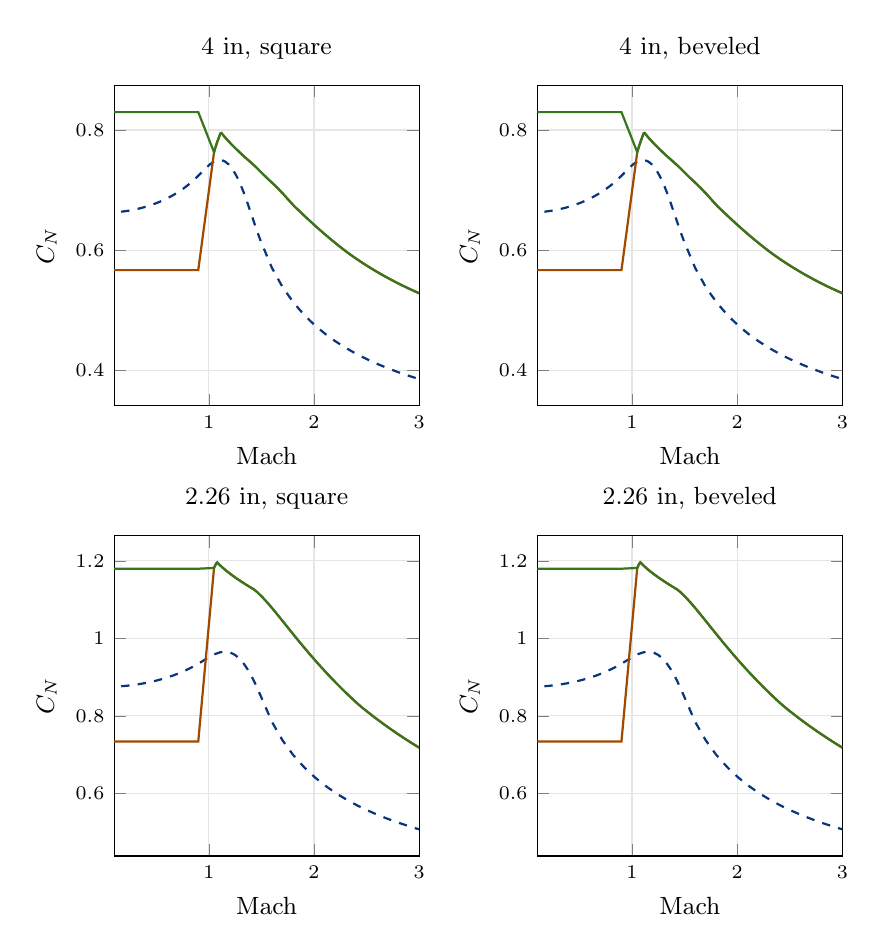
\begin{tikzpicture}
\begin{groupplot}[group style={group size=2 by 2,horizontal sep=1.50cm,vertical sep=1.65cm},width=.45\textwidth,height=5.65cm,grid=major,grid style={gray!20},tick label style={font=\scriptsize},label style={font=\small},title style={font=\small},scaled y ticks=false,yticklabel style={/pgf/number format/fixed,/pgf/number format/precision=3},unbounded coords=jump]
\nextgroupplot[title={4 in, square},xlabel={Mach},ylabel={$C_N$},xmin=0.1,xmax=3]
\addplot[thick,B,dashed] coordinates {(0.01,0.662495) (0.06,0.662702) (0.11,0.6632063) (0.16,0.6640118) (0.21,0.6651249) (0.26,0.6665546) (0.31,0.6683125) (0.36,0.6704135) (0.41,0.6728759) (0.46,0.6757221) (0.51,0.6789793) (0.56,0.6826799) (0.61,0.6868635) (0.66,0.6915776) (0.71,0.6968798) (0.76,0.7028409) (0.81,0.7095479) (0.86,0.7171095) (0.91,0.7256575) (0.96,0.7347275) (1.01,0.7427683) (1.04,0.7464644) (1.06,0.748277) (1.1,0.7500019) (1.11,0.74999) (1.14,0.7487832) (1.16,0.7469512) (1.19,0.7425881) (1.21,0.7385807) (1.23,0.7336929) (1.26,0.7247434) (1.28,0.7177436) (1.31,0.7058172) (1.33,0.6970156) (1.36,0.6827615) (1.41,0.657186) (1.46,0.6314187) (1.49,0.6171275) (1.51,0.6085505) (1.56,0.5876421) (1.6,0.5709154) (1.61,0.5677571) (1.66,0.5519654) (1.7,0.539332) (1.71,0.5368292) (1.76,0.5243155) (1.81,0.5122549) (1.86,0.5020069) (1.91,0.4920892) (1.96,0.4834924) (2.01,0.4751459) (2.06,0.4678001) (2.11,0.4606497) (2.16,0.4542806) (2.21,0.4480677) (2.26,0.4424793) (2.31,0.4370182) (2.36,0.4320662) (2.41,0.4272195) (2.46,0.4227945) (2.51,0.418458) (2.56,0.4144754) (2.61,0.410568) (2.66,0.4069612) (2.71,0.403419) (2.76,0.4001347) (2.81,0.3969062) (2.86,0.393901) (2.91,0.3909445) (2.96,0.3881828) (3,0.3859734)};
\addplot[thick,burntorange] coordinates {(0.01,0.5671165) (0.06,0.5671165) (0.11,0.5671165) (0.16,0.5671165) (0.21,0.5671165) (0.26,0.5671165) (0.31,0.5671165) (0.36,0.5671165) (0.41,0.5671165) (0.46,0.5671165) (0.51,0.5671165) (0.56,0.5671165) (0.61,0.5671165) (0.66,0.5671165) (0.71,0.5671165) (0.76,0.5671165) (0.81,0.5671165) (0.86,0.5671165) (0.9,0.5671165) (0.91,0.5801775) (0.96,0.6454826) (1.01,0.7107877) (1.05,0.7630318) (1.06,0.7691083) (1.08,0.7799721) (1.11,0.7941347) (1.12,0.7949527) (1.16,0.7866162) (1.21,0.7771677) (1.26,0.7684193) (1.31,0.7601473) (1.36,0.7522184) (1.41,0.7445455) (1.43,0.741534) (1.46,0.7363348) (1.51,0.7276231) (1.56,0.7190316) (1.61,0.7109518) (1.66,0.7024354) (1.71,0.6931381) (1.76,0.683421) (1.81,0.6737537) (1.86,0.6654277) (1.91,0.6571568) (1.96,0.6490087) (2.01,0.6410262) (2.06,0.6332358) (2.11,0.6256521) (2.16,0.6182819) (2.21,0.6111267) (2.26,0.6041838) (2.31,0.5974487) (2.36,0.5911064) (2.41,0.5850594) (2.46,0.5792421) (2.51,0.5736452) (2.56,0.56826) (2.61,0.563077) (2.66,0.5580877) (2.71,0.5532831) (2.76,0.5486553) (2.81,0.5441962) (2.86,0.5398984) (2.91,0.5357542) (2.96,0.531757) (3,0.5286606)};
\addplot[thick,g] coordinates {(0.01,0.8297316) (0.06,0.8297316) (0.11,0.8297316) (0.16,0.8297316) (0.21,0.8297316) (0.26,0.8297316) (0.31,0.8297316) (0.36,0.8297316) (0.41,0.8297316) (0.46,0.8297316) (0.51,0.8297316) (0.56,0.8297316) (0.61,0.8297316) (0.66,0.8297316) (0.71,0.8297316) (0.76,0.8297316) (0.81,0.8297316) (0.86,0.8297316) (0.9,0.8297316) (0.91,0.8252849) (0.96,0.8030517) (1.01,0.7808184) (1.05,0.7630318) (1.06,0.7691083) (1.08,0.7799721) (1.11,0.7941347) (1.12,0.7949527) (1.16,0.7866162) (1.21,0.7771677) (1.26,0.7684193) (1.31,0.7601473) (1.36,0.7522184) (1.41,0.7445455) (1.46,0.7363348) (1.51,0.7276231) (1.56,0.7190316) (1.61,0.7109518) (1.66,0.7024354) (1.71,0.6931381) (1.76,0.683421) (1.81,0.6737537) (1.86,0.6654277) (1.91,0.6571568) (1.96,0.6490087) (2.01,0.6410262) (2.06,0.6332358) (2.11,0.6256521) (2.16,0.6182819) (2.21,0.6111267) (2.26,0.6041838) (2.31,0.5974487) (2.36,0.5911064) (2.41,0.5850594) (2.46,0.5792421) (2.51,0.5736452) (2.56,0.56826) (2.61,0.563077) (2.66,0.5580877) (2.71,0.5532831) (2.76,0.5486553) (2.81,0.5441962) (2.86,0.5398984) (2.91,0.5357542) (2.96,0.531757) (3,0.5286606)};
\nextgroupplot[title={4 in, beveled},xlabel={Mach},ylabel={$C_N$},xmin=0.1,xmax=3]
\addplot[thick,B,dashed] coordinates {(0.01,0.662495) (0.06,0.662702) (0.11,0.6632063) (0.16,0.6640118) (0.21,0.6651249) (0.26,0.6665546) (0.31,0.6683125) (0.36,0.6704135) (0.41,0.6728759) (0.46,0.6757221) (0.51,0.6789793) (0.56,0.6826799) (0.61,0.6868635) (0.66,0.6915776) (0.71,0.6968798) (0.76,0.7028409) (0.81,0.7095479) (0.86,0.7171095) (0.91,0.7256575) (0.96,0.7347275) (1.01,0.7427683) (1.04,0.7464644) (1.06,0.748277) (1.1,0.7500019) (1.11,0.74999) (1.14,0.7487832) (1.16,0.7469512) (1.19,0.7425881) (1.21,0.7385807) (1.23,0.7336929) (1.26,0.7247434) (1.28,0.7177436) (1.31,0.7058172) (1.33,0.6970156) (1.36,0.6827615) (1.41,0.657186) (1.46,0.6314187) (1.49,0.6171275) (1.51,0.6085505) (1.56,0.5876421) (1.6,0.5709154) (1.61,0.5677571) (1.66,0.5519654) (1.7,0.539332) (1.71,0.5368292) (1.76,0.5243155) (1.81,0.5122549) (1.86,0.5020069) (1.91,0.4920892) (1.96,0.4834924) (2.01,0.4751459) (2.06,0.4678001) (2.11,0.4606497) (2.16,0.4542806) (2.21,0.4480677) (2.26,0.4424793) (2.31,0.4370182) (2.36,0.4320662) (2.41,0.4272195) (2.46,0.4227945) (2.51,0.418458) (2.56,0.4144754) (2.61,0.410568) (2.66,0.4069612) (2.71,0.403419) (2.76,0.4001347) (2.81,0.3969062) (2.86,0.393901) (2.91,0.3909445) (2.96,0.3881828) (3,0.3859734)};
\addplot[thick,burntorange] coordinates {(0.01,0.5671165) (0.06,0.5671165) (0.11,0.5671165) (0.16,0.5671165) (0.21,0.5671165) (0.26,0.5671165) (0.31,0.5671165) (0.36,0.5671165) (0.41,0.5671165) (0.46,0.5671165) (0.51,0.5671165) (0.56,0.5671165) (0.61,0.5671165) (0.66,0.5671165) (0.71,0.5671165) (0.76,0.5671165) (0.81,0.5671165) (0.86,0.5671165) (0.9,0.5671165) (0.91,0.5801775) (0.96,0.6454826) (1.01,0.7107877) (1.05,0.7630318) (1.06,0.7691083) (1.08,0.7799721) (1.11,0.7941347) (1.12,0.7949527) (1.16,0.7866162) (1.21,0.7771677) (1.26,0.7684193) (1.31,0.7601473) (1.36,0.7522184) (1.41,0.7445455) (1.43,0.741534) (1.46,0.7363348) (1.51,0.7276231) (1.56,0.7190316) (1.61,0.7109518) (1.66,0.7024354) (1.71,0.6931381) (1.76,0.683421) (1.81,0.6737537) (1.86,0.6654277) (1.91,0.6571568) (1.96,0.6490087) (2.01,0.6410262) (2.06,0.6332358) (2.11,0.6256521) (2.16,0.6182819) (2.21,0.6111267) (2.26,0.6041838) (2.31,0.5974487) (2.36,0.5911064) (2.41,0.5850594) (2.46,0.5792421) (2.51,0.5736452) (2.56,0.56826) (2.61,0.563077) (2.66,0.5580877) (2.71,0.5532831) (2.76,0.5486553) (2.81,0.5441962) (2.86,0.5398984) (2.91,0.5357542) (2.96,0.531757) (3,0.5286606)};
\addplot[thick,g] coordinates {(0.01,0.8297316) (0.06,0.8297316) (0.11,0.8297316) (0.16,0.8297316) (0.21,0.8297316) (0.26,0.8297316) (0.31,0.8297316) (0.36,0.8297316) (0.41,0.8297316) (0.46,0.8297316) (0.51,0.8297316) (0.56,0.8297316) (0.61,0.8297316) (0.66,0.8297316) (0.71,0.8297316) (0.76,0.8297316) (0.81,0.8297316) (0.86,0.8297316) (0.9,0.8297316) (0.91,0.8252849) (0.96,0.8030517) (1.01,0.7808184) (1.05,0.7630318) (1.06,0.7691083) (1.08,0.7799721) (1.11,0.7941347) (1.12,0.7949527) (1.16,0.7866162) (1.21,0.7771677) (1.26,0.7684193) (1.31,0.7601473) (1.36,0.7522184) (1.41,0.7445455) (1.46,0.7363348) (1.51,0.7276231) (1.56,0.7190316) (1.61,0.7109518) (1.66,0.7024354) (1.71,0.6931381) (1.76,0.683421) (1.81,0.6737537) (1.86,0.6654277) (1.91,0.6571568) (1.96,0.6490087) (2.01,0.6410262) (2.06,0.6332358) (2.11,0.6256521) (2.16,0.6182819) (2.21,0.6111267) (2.26,0.6041838) (2.31,0.5974487) (2.36,0.5911064) (2.41,0.5850594) (2.46,0.5792421) (2.51,0.5736452) (2.56,0.56826) (2.61,0.563077) (2.66,0.5580877) (2.71,0.5532831) (2.76,0.5486553) (2.81,0.5441962) (2.86,0.5398984) (2.91,0.5357542) (2.96,0.531757) (3,0.5286606)};
\nextgroupplot[title={2.26 in, square},xlabel={Mach},ylabel={$C_N$},xmin=0.1,xmax=3]
\addplot[thick,B,dashed] coordinates {(0.01,0.8746562) (0.06,0.8748721) (0.11,0.8753976) (0.16,0.8762359) (0.21,0.8773921) (0.26,0.878873) (0.31,0.880688) (0.36,0.8828484) (0.41,0.8853683) (0.46,0.8882645) (0.51,0.891557) (0.56,0.8952697) (0.61,0.8994304) (0.66,0.9040721) (0.71,0.9092337) (0.76,0.914961) (0.81,0.9213088) (0.86,0.9283421) (0.91,0.9361391) (0.96,0.9445425) (1.01,0.9526984) (1.06,0.9595845) (1.11,0.9641709) (1.15,0.9655251) (1.16,0.9654818) (1.19,0.9643318) (1.21,0.9626576) (1.24,0.9586856) (1.26,0.955017) (1.29,0.9479255) (1.31,0.9421191) (1.33,0.9354452) (1.36,0.9238251) (1.38,0.9150335) (1.41,0.9003607) (1.43,0.8896576) (1.46,0.872378) (1.51,0.8412081) (1.56,0.8098123) (1.6,0.7846958) (1.61,0.7799532) (1.66,0.7562406) (1.7,0.7372704) (1.71,0.7335123) (1.76,0.7147218) (1.8,0.6996894) (1.81,0.6966118) (1.86,0.6812236) (1.91,0.6663312) (1.96,0.6534224) (2.01,0.6408893) (2.06,0.6298591) (2.11,0.6191221) (2.16,0.6095583) (2.21,0.6002291) (2.26,0.5918376) (2.31,0.5836373) (2.36,0.5762014) (2.41,0.5689237) (2.46,0.5622792) (2.51,0.5557675) (2.56,0.5497873) (2.61,0.54392) (2.66,0.5385042) (2.71,0.5331851) (2.76,0.5282535) (2.81,0.5234056) (2.86,0.5188931) (2.91,0.5144536) (2.96,0.5103067) (3,0.5069892)};
\addplot[thick,burntorange] coordinates {(0.01,0.7339886) (0.06,0.7339886) (0.11,0.7339886) (0.16,0.7339886) (0.21,0.7339886) (0.26,0.7339886) (0.31,0.7339886) (0.36,0.7339886) (0.41,0.7339886) (0.46,0.7339886) (0.51,0.7339886) (0.56,0.7339886) (0.61,0.7339886) (0.66,0.7339886) (0.71,0.7339886) (0.76,0.7339886) (0.81,0.7339886) (0.86,0.7339886) (0.9,0.7339886) (0.91,0.7638429) (0.96,0.9131143) (1.01,1.062386) (1.05,1.181803) (1.06,1.187797) (1.07,1.193343) (1.08,1.196142) (1.11,1.187868) (1.16,1.175913) (1.21,1.165327) (1.26,1.155603) (1.31,1.146473) (1.36,1.13778) (1.41,1.12942) (1.43,1.126196) (1.46,1.119502) (1.51,1.106278) (1.56,1.091398) (1.61,1.075447) (1.66,1.05887) (1.71,1.04199) (1.76,1.025042) (1.81,1.00819) (1.86,0.9915472) (1.91,0.9751928) (1.96,0.9591775) (2.01,0.943534) (2.06,0.9282813) (2.11,0.9134274) (2.16,0.8989735) (2.21,0.8849165) (2.26,0.8712487) (2.31,0.8579603) (2.36,0.8450397) (2.41,0.8324748) (2.46,0.8208934) (2.51,0.8099956) (2.56,0.7994094) (2.61,0.7891224) (2.66,0.7791214) (2.71,0.7693946) (2.76,0.7599292) (2.81,0.7507139) (2.86,0.7417378) (2.91,0.73299) (2.96,0.7244602) (3,0.7177867)};
\addplot[thick,g] coordinates {(0.01,1.179858) (0.06,1.179858) (0.11,1.179858) (0.16,1.179858) (0.21,1.179858) (0.26,1.179858) (0.31,1.179858) (0.36,1.179858) (0.41,1.179858) (0.46,1.179858) (0.51,1.179858) (0.56,1.179858) (0.61,1.179858) (0.66,1.179858) (0.71,1.179858) (0.76,1.179858) (0.81,1.179858) (0.86,1.179858) (0.91,1.179988) (0.96,1.180636) (1.01,1.181284) (1.05,1.181803) (1.06,1.187797) (1.07,1.193343) (1.08,1.196142) (1.11,1.187868) (1.16,1.175913) (1.21,1.165327) (1.26,1.155603) (1.31,1.146473) (1.36,1.13778) (1.41,1.12942) (1.43,1.126196) (1.46,1.119502) (1.51,1.106278) (1.56,1.091398) (1.61,1.075447) (1.66,1.05887) (1.71,1.04199) (1.76,1.025042) (1.81,1.00819) (1.86,0.9915472) (1.91,0.9751928) (1.96,0.9591775) (2.01,0.943534) (2.06,0.9282813) (2.11,0.9134274) (2.16,0.8989735) (2.21,0.8849165) (2.26,0.8712487) (2.31,0.8579603) (2.36,0.8450397) (2.41,0.8324748) (2.46,0.8208934) (2.51,0.8099956) (2.56,0.7994094) (2.61,0.7891224) (2.66,0.7791214) (2.71,0.7693946) (2.76,0.7599292) (2.81,0.7507139) (2.86,0.7417378) (2.91,0.73299) (2.96,0.7244602) (3,0.7177867)};
\nextgroupplot[title={2.26 in, beveled},xlabel={Mach},ylabel={$C_N$},xmin=0.1,xmax=3]
\addplot[thick,B,dashed] coordinates {(0.01,0.8746562) (0.06,0.8748721) (0.11,0.8753976) (0.16,0.8762359) (0.21,0.8773921) (0.26,0.878873) (0.31,0.880688) (0.36,0.8828484) (0.41,0.8853683) (0.46,0.8882645) (0.51,0.891557) (0.56,0.8952697) (0.61,0.8994304) (0.66,0.9040721) (0.71,0.9092337) (0.76,0.914961) (0.81,0.9213088) (0.86,0.9283421) (0.91,0.9361391) (0.96,0.9445425) (1.01,0.9526984) (1.06,0.9595845) (1.11,0.9641709) (1.15,0.9655251) (1.16,0.9654818) (1.19,0.9643318) (1.21,0.9626576) (1.24,0.9586856) (1.26,0.955017) (1.29,0.9479255) (1.31,0.9421191) (1.33,0.9354452) (1.36,0.9238251) (1.38,0.9150335) (1.41,0.9003607) (1.43,0.8896576) (1.46,0.872378) (1.51,0.8412081) (1.56,0.8098123) (1.6,0.7846958) (1.61,0.7799532) (1.66,0.7562406) (1.7,0.7372704) (1.71,0.7335123) (1.76,0.7147218) (1.8,0.6996894) (1.81,0.6966118) (1.86,0.6812236) (1.91,0.6663312) (1.96,0.6534224) (2.01,0.6408893) (2.06,0.6298591) (2.11,0.6191221) (2.16,0.6095583) (2.21,0.6002291) (2.26,0.5918376) (2.31,0.5836373) (2.36,0.5762014) (2.41,0.5689237) (2.46,0.5622792) (2.51,0.5557675) (2.56,0.5497873) (2.61,0.54392) (2.66,0.5385042) (2.71,0.5331851) (2.76,0.5282535) (2.81,0.5234056) (2.86,0.5188931) (2.91,0.5144536) (2.96,0.5103067) (3,0.5069892)};
\addplot[thick,burntorange] coordinates {(0.01,0.7339886) (0.06,0.7339886) (0.11,0.7339886) (0.16,0.7339886) (0.21,0.7339886) (0.26,0.7339886) (0.31,0.7339886) (0.36,0.7339886) (0.41,0.7339886) (0.46,0.7339886) (0.51,0.7339886) (0.56,0.7339886) (0.61,0.7339886) (0.66,0.7339886) (0.71,0.7339886) (0.76,0.7339886) (0.81,0.7339886) (0.86,0.7339886) (0.9,0.7339886) (0.91,0.7638429) (0.96,0.9131143) (1.01,1.062386) (1.05,1.181803) (1.06,1.187797) (1.07,1.193343) (1.08,1.196142) (1.11,1.187868) (1.16,1.175913) (1.21,1.165327) (1.26,1.155603) (1.31,1.146473) (1.36,1.13778) (1.41,1.12942) (1.43,1.126196) (1.46,1.119502) (1.51,1.106278) (1.56,1.091398) (1.61,1.075447) (1.66,1.05887) (1.71,1.04199) (1.76,1.025042) (1.81,1.00819) (1.86,0.9915472) (1.91,0.9751928) (1.96,0.9591775) (2.01,0.943534) (2.06,0.9282813) (2.11,0.9134274) (2.16,0.8989735) (2.21,0.8849165) (2.26,0.8712487) (2.31,0.8579603) (2.36,0.8450397) (2.41,0.8324748) (2.46,0.8208934) (2.51,0.8099956) (2.56,0.7994094) (2.61,0.7891224) (2.66,0.7791214) (2.71,0.7693946) (2.76,0.7599292) (2.81,0.7507139) (2.86,0.7417378) (2.91,0.73299) (2.96,0.7244602) (3,0.7177867)};
\addplot[thick,g] coordinates {(0.01,1.179858) (0.06,1.179858) (0.11,1.179858) (0.16,1.179858) (0.21,1.179858) (0.26,1.179858) (0.31,1.179858) (0.36,1.179858) (0.41,1.179858) (0.46,1.179858) (0.51,1.179858) (0.56,1.179858) (0.61,1.179858) (0.66,1.179858) (0.71,1.179858) (0.76,1.179858) (0.81,1.179858) (0.86,1.179858) (0.91,1.179988) (0.96,1.180636) (1.01,1.181284) (1.05,1.181803) (1.06,1.187797) (1.07,1.193343) (1.08,1.196142) (1.11,1.187868) (1.16,1.175913) (1.21,1.165327) (1.26,1.155603) (1.31,1.146473) (1.36,1.13778) (1.41,1.12942) (1.43,1.126196) (1.46,1.119502) (1.51,1.106278) (1.56,1.091398) (1.61,1.075447) (1.66,1.05887) (1.71,1.04199) (1.76,1.025042) (1.81,1.00819) (1.86,0.9915472) (1.91,0.9751928) (1.96,0.9591775) (2.01,0.943534) (2.06,0.9282813) (2.11,0.9134274) (2.16,0.8989735) (2.21,0.8849165) (2.26,0.8712487) (2.31,0.8579603) (2.36,0.8450397) (2.41,0.8324748) (2.46,0.8208934) (2.51,0.8099956) (2.56,0.7994094) (2.61,0.7891224) (2.66,0.7791214) (2.71,0.7693946) (2.76,0.7599292) (2.81,0.7507139) (2.86,0.7417378) (2.91,0.73299) (2.96,0.7244602) (3,0.7177867)};
\end{groupplot}\end{tikzpicture}
\caption{Default and modified RAS settings share geometry and drag-flow inputs. This isolates the normal-force/body-interference option, compared with unmodified MIT OR.}\label{fig:atlas-26-rogers-CN}
\end{figure}
\noindent{\footnotesize Export files: \code{26-rogers-CN.svg} and \code{26-rogers-CN.png}.\\ Directory: \code{aerodynamic-investigation/extended/figures/}.}

\clearpage\subsubsection*{Rogers Modified Barrowman: CP at 4 degrees}
\begin{figure}[H]\centering
{\footnotesize\begin{tabular}{lll}
\tikz[baseline=-.5ex]{\draw[thick,B,dashed] (0,0)--(.40,0);}\ MIT OR & \tikz[baseline=-.5ex]{\draw[thick,burntorange] (0,0)--(.40,0);}\ RAS default & \tikz[baseline=-.5ex]{\draw[thick,g] (0,0)--(.40,0);}\ RAS Rogers modified\\
\end{tabular}}\par\vspace{.7em}
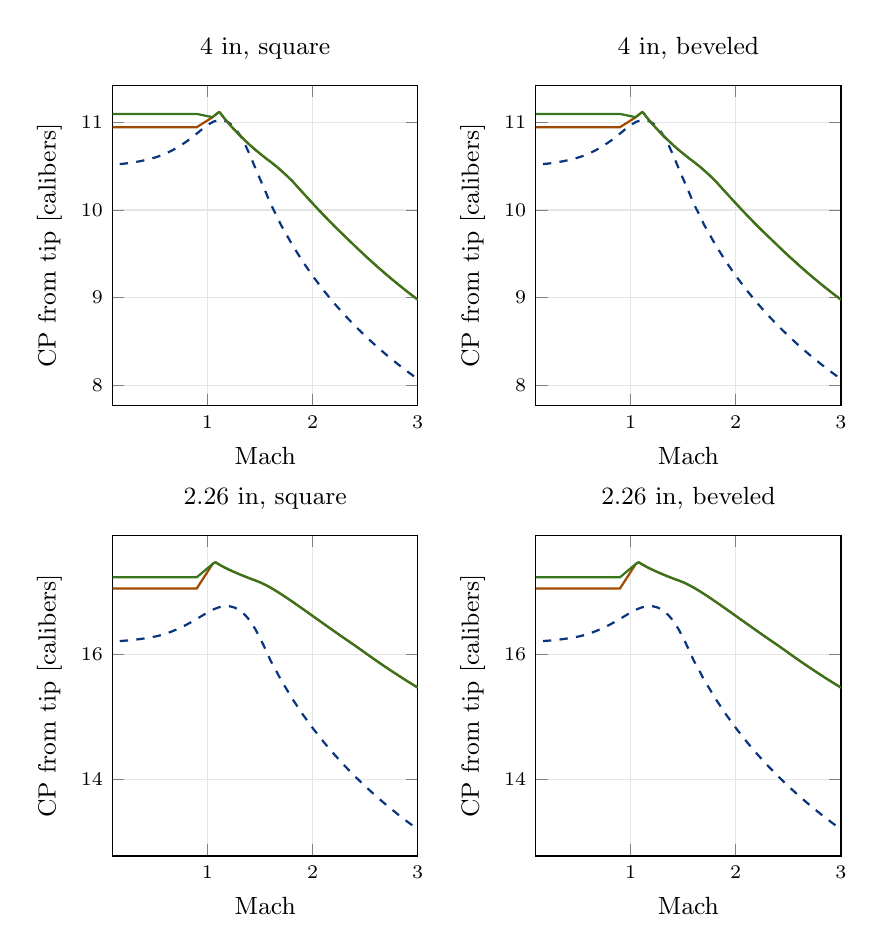
\begin{tikzpicture}
\begin{groupplot}[group style={group size=2 by 2,horizontal sep=1.50cm,vertical sep=1.65cm},width=.45\textwidth,height=5.65cm,grid=major,grid style={gray!20},tick label style={font=\scriptsize},label style={font=\small},title style={font=\small},scaled y ticks=false,yticklabel style={/pgf/number format/fixed,/pgf/number format/precision=3},unbounded coords=jump]
\nextgroupplot[title={4 in, square},xlabel={Mach},ylabel={CP from tip [calibers]},xmin=0.1,xmax=3]
\addplot[thick,B,dashed] coordinates {(0.01,10.5144) (0.06,10.51551) (0.11,10.51821) (0.16,10.5225) (0.21,10.52842) (0.26,10.536) (0.31,10.54526) (0.36,10.55628) (0.41,10.5691) (0.46,10.5838) (0.51,10.60054) (0.56,10.6212) (0.61,10.64639) (0.66,10.6758) (0.71,10.70919) (0.76,10.74643) (0.81,10.78745) (0.86,10.83228) (0.91,10.88106) (0.96,10.93126) (1.01,10.97589) (1.06,11.00873) (1.11,11.02477) (1.12,11.02559) (1.16,11.01999) (1.19,11.00578) (1.21,10.99124) (1.24,10.96147) (1.26,10.93619) (1.28,10.9065) (1.31,10.85367) (1.33,10.81303) (1.36,10.74436) (1.41,10.6123) (1.46,10.46726) (1.51,10.32772) (1.56,10.19009) (1.6,10.07221) (1.61,10.04922) (1.66,9.930043) (1.7,9.829356) (1.71,9.808874) (1.76,9.703352) (1.81,9.596574) (1.86,9.501802) (1.91,9.406233) (1.96,9.320257) (2.01,9.233773) (2.06,9.155104) (2.11,9.076029) (2.16,9.003484) (2.21,8.930664) (2.26,8.863406) (2.31,8.795967) (2.36,8.733331) (2.41,8.670583) (2.46,8.612029) (2.51,8.553412) (2.56,8.498494) (2.61,8.44355) (2.66,8.391893) (2.71,8.340239) (2.76,8.291525) (2.81,8.242836) (2.86,8.196793) (2.91,8.150791) (2.96,8.107184) (3,8.071837)};
\addplot[thick,burntorange] coordinates {(0.01,10.94443) (0.06,10.94443) (0.11,10.94443) (0.16,10.94443) (0.21,10.94443) (0.26,10.94443) (0.31,10.94443) (0.36,10.94443) (0.41,10.94443) (0.46,10.94443) (0.51,10.94443) (0.56,10.94443) (0.61,10.94443) (0.66,10.94443) (0.71,10.94443) (0.76,10.94443) (0.81,10.94443) (0.86,10.94443) (0.9,10.94443) (0.91,10.95199) (0.96,10.98978) (1.01,11.02758) (1.05,11.05781) (1.06,11.06903) (1.11,11.11606) (1.12,11.11081) (1.16,11.04772) (1.21,10.97676) (1.26,10.91149) (1.31,10.85009) (1.36,10.79148) (1.41,10.73493) (1.46,10.68265) (1.51,10.6339) (1.56,10.586) (1.61,10.54086) (1.66,10.49317) (1.71,10.44079) (1.76,10.38537) (1.81,10.32689) (1.86,10.26066) (1.91,10.19444) (1.96,10.12863) (2.01,10.06352) (2.06,9.999335) (2.11,9.936226) (2.16,9.87431) (2.21,9.813674) (2.26,9.754379) (2.31,9.696467) (2.36,9.639028) (2.41,9.58106) (2.46,9.524123) (2.51,9.468236) (2.56,9.413416) (2.61,9.359669) (2.66,9.307009) (2.71,9.255433) (2.76,9.204946) (2.81,9.155547) (2.86,9.107232) (2.91,9.059999) (2.96,9.013842) (3,8.977689)};
\addplot[thick,g] coordinates {(0.01,11.09545) (0.06,11.09545) (0.11,11.09545) (0.16,11.09545) (0.21,11.09545) (0.26,11.09545) (0.31,11.09545) (0.36,11.09545) (0.41,11.09545) (0.46,11.09545) (0.51,11.09545) (0.56,11.09545) (0.61,11.09545) (0.66,11.09545) (0.71,11.09545) (0.76,11.09545) (0.81,11.09545) (0.86,11.09545) (0.91,11.09294) (0.96,11.0804) (1.01,11.06785) (1.05,11.05781) (1.06,11.06903) (1.11,11.11606) (1.12,11.11081) (1.16,11.04772) (1.21,10.97676) (1.26,10.91149) (1.31,10.85009) (1.36,10.79148) (1.41,10.73493) (1.46,10.68265) (1.51,10.6339) (1.56,10.586) (1.61,10.54086) (1.66,10.49317) (1.71,10.44079) (1.76,10.38537) (1.81,10.32689) (1.86,10.26066) (1.91,10.19444) (1.96,10.12863) (2.01,10.06352) (2.06,9.999335) (2.11,9.936226) (2.16,9.87431) (2.21,9.813674) (2.26,9.754379) (2.31,9.696467) (2.36,9.639028) (2.41,9.58106) (2.46,9.524123) (2.51,9.468236) (2.56,9.413416) (2.61,9.359669) (2.66,9.307009) (2.71,9.255433) (2.76,9.204946) (2.81,9.155547) (2.86,9.107232) (2.91,9.059999) (2.96,9.013842) (3,8.977689)};
\nextgroupplot[title={4 in, beveled},xlabel={Mach},ylabel={CP from tip [calibers]},xmin=0.1,xmax=3]
\addplot[thick,B,dashed] coordinates {(0.01,10.5144) (0.06,10.51551) (0.11,10.51821) (0.16,10.5225) (0.21,10.52842) (0.26,10.536) (0.31,10.54526) (0.36,10.55628) (0.41,10.5691) (0.46,10.5838) (0.51,10.60054) (0.56,10.6212) (0.61,10.64639) (0.66,10.6758) (0.71,10.70919) (0.76,10.74643) (0.81,10.78745) (0.86,10.83228) (0.91,10.88106) (0.96,10.93126) (1.01,10.97589) (1.06,11.00873) (1.11,11.02477) (1.12,11.02559) (1.16,11.01999) (1.19,11.00578) (1.21,10.99124) (1.24,10.96147) (1.26,10.93619) (1.28,10.9065) (1.31,10.85367) (1.33,10.81303) (1.36,10.74436) (1.41,10.6123) (1.46,10.46726) (1.51,10.32772) (1.56,10.19009) (1.6,10.07221) (1.61,10.04922) (1.66,9.930043) (1.7,9.829356) (1.71,9.808874) (1.76,9.703352) (1.81,9.596574) (1.86,9.501802) (1.91,9.406233) (1.96,9.320257) (2.01,9.233773) (2.06,9.155104) (2.11,9.076029) (2.16,9.003484) (2.21,8.930664) (2.26,8.863406) (2.31,8.795967) (2.36,8.733331) (2.41,8.670583) (2.46,8.612029) (2.51,8.553412) (2.56,8.498494) (2.61,8.44355) (2.66,8.391893) (2.71,8.340239) (2.76,8.291525) (2.81,8.242836) (2.86,8.196793) (2.91,8.150791) (2.96,8.107184) (3,8.071837)};
\addplot[thick,burntorange] coordinates {(0.01,10.94443) (0.06,10.94443) (0.11,10.94443) (0.16,10.94443) (0.21,10.94443) (0.26,10.94443) (0.31,10.94443) (0.36,10.94443) (0.41,10.94443) (0.46,10.94443) (0.51,10.94443) (0.56,10.94443) (0.61,10.94443) (0.66,10.94443) (0.71,10.94443) (0.76,10.94443) (0.81,10.94443) (0.86,10.94443) (0.9,10.94443) (0.91,10.95199) (0.96,10.98978) (1.01,11.02758) (1.05,11.05781) (1.06,11.06903) (1.11,11.11606) (1.12,11.11081) (1.16,11.04772) (1.21,10.97676) (1.26,10.91149) (1.31,10.85009) (1.36,10.79148) (1.41,10.73493) (1.46,10.68265) (1.51,10.6339) (1.56,10.586) (1.61,10.54086) (1.66,10.49317) (1.71,10.44079) (1.76,10.38537) (1.81,10.32689) (1.86,10.26066) (1.91,10.19444) (1.96,10.12863) (2.01,10.06352) (2.06,9.999335) (2.11,9.936226) (2.16,9.87431) (2.21,9.813674) (2.26,9.754379) (2.31,9.696467) (2.36,9.639028) (2.41,9.58106) (2.46,9.524123) (2.51,9.468236) (2.56,9.413416) (2.61,9.359669) (2.66,9.307009) (2.71,9.255433) (2.76,9.204946) (2.81,9.155547) (2.86,9.107232) (2.91,9.059999) (2.96,9.013842) (3,8.977689)};
\addplot[thick,g] coordinates {(0.01,11.09545) (0.06,11.09545) (0.11,11.09545) (0.16,11.09545) (0.21,11.09545) (0.26,11.09545) (0.31,11.09545) (0.36,11.09545) (0.41,11.09545) (0.46,11.09545) (0.51,11.09545) (0.56,11.09545) (0.61,11.09545) (0.66,11.09545) (0.71,11.09545) (0.76,11.09545) (0.81,11.09545) (0.86,11.09545) (0.91,11.09294) (0.96,11.0804) (1.01,11.06785) (1.05,11.05781) (1.06,11.06903) (1.11,11.11606) (1.12,11.11081) (1.16,11.04772) (1.21,10.97676) (1.26,10.91149) (1.31,10.85009) (1.36,10.79148) (1.41,10.73493) (1.46,10.68265) (1.51,10.6339) (1.56,10.586) (1.61,10.54086) (1.66,10.49317) (1.71,10.44079) (1.76,10.38537) (1.81,10.32689) (1.86,10.26066) (1.91,10.19444) (1.96,10.12863) (2.01,10.06352) (2.06,9.999335) (2.11,9.936226) (2.16,9.87431) (2.21,9.813674) (2.26,9.754379) (2.31,9.696467) (2.36,9.639028) (2.41,9.58106) (2.46,9.524123) (2.51,9.468236) (2.56,9.413416) (2.61,9.359669) (2.66,9.307009) (2.71,9.255433) (2.76,9.204946) (2.81,9.155547) (2.86,9.107232) (2.91,9.059999) (2.96,9.013842) (3,8.977689)};
\nextgroupplot[title={2.26 in, square},xlabel={Mach},ylabel={CP from tip [calibers]},xmin=0.1,xmax=3]
\addplot[thick,B,dashed] coordinates {(0.01,16.20243) (0.06,16.20351) (0.11,16.20613) (0.16,16.21031) (0.21,16.21606) (0.26,16.2234) (0.31,16.23236) (0.36,16.24298) (0.41,16.25531) (0.46,16.26938) (0.51,16.28537) (0.56,16.30598) (0.61,16.33203) (0.66,16.3629) (0.71,16.39811) (0.76,16.43723) (0.81,16.47993) (0.86,16.52599) (0.91,16.57526) (0.96,16.62659) (1.01,16.67596) (1.06,16.71893) (1.11,16.75123) (1.16,16.76892) (1.18,16.77109) (1.21,16.76838) (1.26,16.74627) (1.31,16.69961) (1.36,16.62578) (1.39,16.56758) (1.41,16.52281) (1.43,16.47321) (1.46,16.38983) (1.51,16.22912) (1.56,16.0534) (1.6,15.90188) (1.61,15.87227) (1.66,15.71817) (1.7,15.58722) (1.71,15.56054) (1.76,15.42259) (1.8,15.30659) (1.81,15.28227) (1.86,15.15719) (1.91,15.03048) (1.96,14.91606) (2.01,14.80048) (2.06,14.69496) (2.11,14.58845) (2.16,14.49038) (2.21,14.39158) (2.26,14.30001) (2.31,14.20789) (2.36,14.12206) (2.41,14.03581) (2.46,13.95509) (2.51,13.87405) (2.56,13.79792) (2.61,13.72155) (2.66,13.64956) (2.71,13.57739) (2.76,13.50918) (2.81,13.44083) (2.86,13.37605) (2.91,13.31118) (2.96,13.24956) (3,13.19952)};
\addplot[thick,burntorange] coordinates {(0.01,17.05341) (0.06,17.05341) (0.11,17.05341) (0.16,17.05341) (0.21,17.05341) (0.26,17.05341) (0.31,17.05341) (0.36,17.05341) (0.41,17.05341) (0.46,17.05341) (0.51,17.05341) (0.56,17.05341) (0.61,17.05341) (0.66,17.05341) (0.71,17.05341) (0.76,17.05341) (0.81,17.05341) (0.86,17.05341) (0.9,17.05341) (0.91,17.07944) (0.96,17.20958) (1.01,17.33973) (1.05,17.44384) (1.06,17.45523) (1.07,17.46581) (1.08,17.46946) (1.11,17.43755) (1.16,17.39124) (1.21,17.35001) (1.26,17.31193) (1.31,17.276) (1.36,17.24159) (1.41,17.20832) (1.46,17.17843) (1.51,17.14435) (1.56,17.10313) (1.61,17.05652) (1.66,17.0059) (1.71,16.95229) (1.76,16.89651) (1.81,16.83916) (1.86,16.78072) (1.91,16.72155) (1.96,16.66193) (2.01,16.6021) (2.06,16.54223) (2.11,16.48248) (2.16,16.42294) (2.21,16.36372) (2.26,16.30488) (2.31,16.2465) (2.36,16.18861) (2.41,16.13126) (2.46,16.0716) (2.51,16.01113) (2.56,15.95153) (2.61,15.89283) (2.66,15.83503) (2.71,15.77815) (2.76,15.7222) (2.81,15.66718) (2.86,15.61311) (2.91,15.55998) (2.96,15.5078) (3,15.46674)};
\addplot[thick,g] coordinates {(0.01,17.2318) (0.06,17.2318) (0.11,17.2318) (0.16,17.2318) (0.21,17.2318) (0.26,17.2318) (0.31,17.2318) (0.36,17.2318) (0.41,17.2318) (0.46,17.2318) (0.51,17.2318) (0.56,17.2318) (0.61,17.2318) (0.66,17.2318) (0.71,17.2318) (0.76,17.2318) (0.81,17.2318) (0.86,17.2318) (0.9,17.2318) (0.91,17.24594) (0.96,17.31662) (1.01,17.3873) (1.05,17.44384) (1.06,17.45523) (1.07,17.46581) (1.08,17.46946) (1.11,17.43755) (1.16,17.39124) (1.21,17.35001) (1.26,17.31193) (1.31,17.276) (1.36,17.24159) (1.41,17.20832) (1.46,17.17843) (1.51,17.14435) (1.56,17.10313) (1.61,17.05652) (1.66,17.0059) (1.71,16.95229) (1.76,16.89651) (1.81,16.83916) (1.86,16.78072) (1.91,16.72155) (1.96,16.66193) (2.01,16.6021) (2.06,16.54223) (2.11,16.48248) (2.16,16.42294) (2.21,16.36372) (2.26,16.30488) (2.31,16.2465) (2.36,16.18861) (2.41,16.13126) (2.46,16.0716) (2.51,16.01113) (2.56,15.95153) (2.61,15.89283) (2.66,15.83503) (2.71,15.77815) (2.76,15.7222) (2.81,15.66718) (2.86,15.61311) (2.91,15.55998) (2.96,15.5078) (3,15.46674)};
\nextgroupplot[title={2.26 in, beveled},xlabel={Mach},ylabel={CP from tip [calibers]},xmin=0.1,xmax=3]
\addplot[thick,B,dashed] coordinates {(0.01,16.20243) (0.06,16.20351) (0.11,16.20613) (0.16,16.21031) (0.21,16.21606) (0.26,16.2234) (0.31,16.23236) (0.36,16.24298) (0.41,16.25531) (0.46,16.26938) (0.51,16.28537) (0.56,16.30598) (0.61,16.33203) (0.66,16.3629) (0.71,16.39811) (0.76,16.43723) (0.81,16.47993) (0.86,16.52599) (0.91,16.57526) (0.96,16.62659) (1.01,16.67596) (1.06,16.71893) (1.11,16.75123) (1.16,16.76892) (1.18,16.77109) (1.21,16.76838) (1.26,16.74627) (1.31,16.69961) (1.36,16.62578) (1.39,16.56758) (1.41,16.52281) (1.43,16.47321) (1.46,16.38983) (1.51,16.22912) (1.56,16.0534) (1.6,15.90188) (1.61,15.87227) (1.66,15.71817) (1.7,15.58722) (1.71,15.56054) (1.76,15.42259) (1.8,15.30659) (1.81,15.28227) (1.86,15.15719) (1.91,15.03048) (1.96,14.91606) (2.01,14.80048) (2.06,14.69496) (2.11,14.58845) (2.16,14.49038) (2.21,14.39158) (2.26,14.30001) (2.31,14.20789) (2.36,14.12206) (2.41,14.03581) (2.46,13.95509) (2.51,13.87405) (2.56,13.79792) (2.61,13.72155) (2.66,13.64956) (2.71,13.57739) (2.76,13.50918) (2.81,13.44083) (2.86,13.37605) (2.91,13.31118) (2.96,13.24956) (3,13.19952)};
\addplot[thick,burntorange] coordinates {(0.01,17.05341) (0.06,17.05341) (0.11,17.05341) (0.16,17.05341) (0.21,17.05341) (0.26,17.05341) (0.31,17.05341) (0.36,17.05341) (0.41,17.05341) (0.46,17.05341) (0.51,17.05341) (0.56,17.05341) (0.61,17.05341) (0.66,17.05341) (0.71,17.05341) (0.76,17.05341) (0.81,17.05341) (0.86,17.05341) (0.9,17.05341) (0.91,17.07944) (0.96,17.20958) (1.01,17.33973) (1.05,17.44384) (1.06,17.45523) (1.07,17.46581) (1.08,17.46946) (1.11,17.43755) (1.16,17.39124) (1.21,17.35001) (1.26,17.31193) (1.31,17.276) (1.36,17.24159) (1.41,17.20832) (1.46,17.17843) (1.51,17.14435) (1.56,17.10313) (1.61,17.05652) (1.66,17.0059) (1.71,16.95229) (1.76,16.89651) (1.81,16.83916) (1.86,16.78072) (1.91,16.72155) (1.96,16.66193) (2.01,16.6021) (2.06,16.54223) (2.11,16.48248) (2.16,16.42294) (2.21,16.36372) (2.26,16.30488) (2.31,16.2465) (2.36,16.18861) (2.41,16.13126) (2.46,16.0716) (2.51,16.01113) (2.56,15.95153) (2.61,15.89283) (2.66,15.83503) (2.71,15.77815) (2.76,15.7222) (2.81,15.66718) (2.86,15.61311) (2.91,15.55998) (2.96,15.5078) (3,15.46674)};
\addplot[thick,g] coordinates {(0.01,17.2318) (0.06,17.2318) (0.11,17.2318) (0.16,17.2318) (0.21,17.2318) (0.26,17.2318) (0.31,17.2318) (0.36,17.2318) (0.41,17.2318) (0.46,17.2318) (0.51,17.2318) (0.56,17.2318) (0.61,17.2318) (0.66,17.2318) (0.71,17.2318) (0.76,17.2318) (0.81,17.2318) (0.86,17.2318) (0.9,17.2318) (0.91,17.24594) (0.96,17.31662) (1.01,17.3873) (1.05,17.44384) (1.06,17.45523) (1.07,17.46581) (1.08,17.46946) (1.11,17.43755) (1.16,17.39124) (1.21,17.35001) (1.26,17.31193) (1.31,17.276) (1.36,17.24159) (1.41,17.20832) (1.46,17.17843) (1.51,17.14435) (1.56,17.10313) (1.61,17.05652) (1.66,17.0059) (1.71,16.95229) (1.76,16.89651) (1.81,16.83916) (1.86,16.78072) (1.91,16.72155) (1.96,16.66193) (2.01,16.6021) (2.06,16.54223) (2.11,16.48248) (2.16,16.42294) (2.21,16.36372) (2.26,16.30488) (2.31,16.2465) (2.36,16.18861) (2.41,16.13126) (2.46,16.0716) (2.51,16.01113) (2.56,15.95153) (2.61,15.89283) (2.66,15.83503) (2.71,15.77815) (2.76,15.7222) (2.81,15.66718) (2.86,15.61311) (2.91,15.55998) (2.96,15.5078) (3,15.46674)};
\end{groupplot}\end{tikzpicture}
\caption{Default and modified RAS settings share geometry and drag-flow inputs. This isolates the normal-force/body-interference option, compared with unmodified MIT OR.}\label{fig:atlas-26-rogers-CP}
\end{figure}
\noindent{\footnotesize Export files: \code{26-rogers-CP.svg} and \code{26-rogers-CP.png}.\\ Directory: \code{aerodynamic-investigation/extended/figures/}.}

\clearpage\subsubsection*{Rogers Modified Barrowman: CD at 4 degrees}
\begin{figure}[H]\centering
{\footnotesize\begin{tabular}{lll}
\tikz[baseline=-.5ex]{\draw[thick,B,dashed] (0,0)--(.40,0);}\ MIT OR & \tikz[baseline=-.5ex]{\draw[thick,burntorange] (0,0)--(.40,0);}\ RAS default & \tikz[baseline=-.5ex]{\draw[thick,g] (0,0)--(.40,0);}\ RAS Rogers modified\\
\end{tabular}}\par\vspace{.7em}
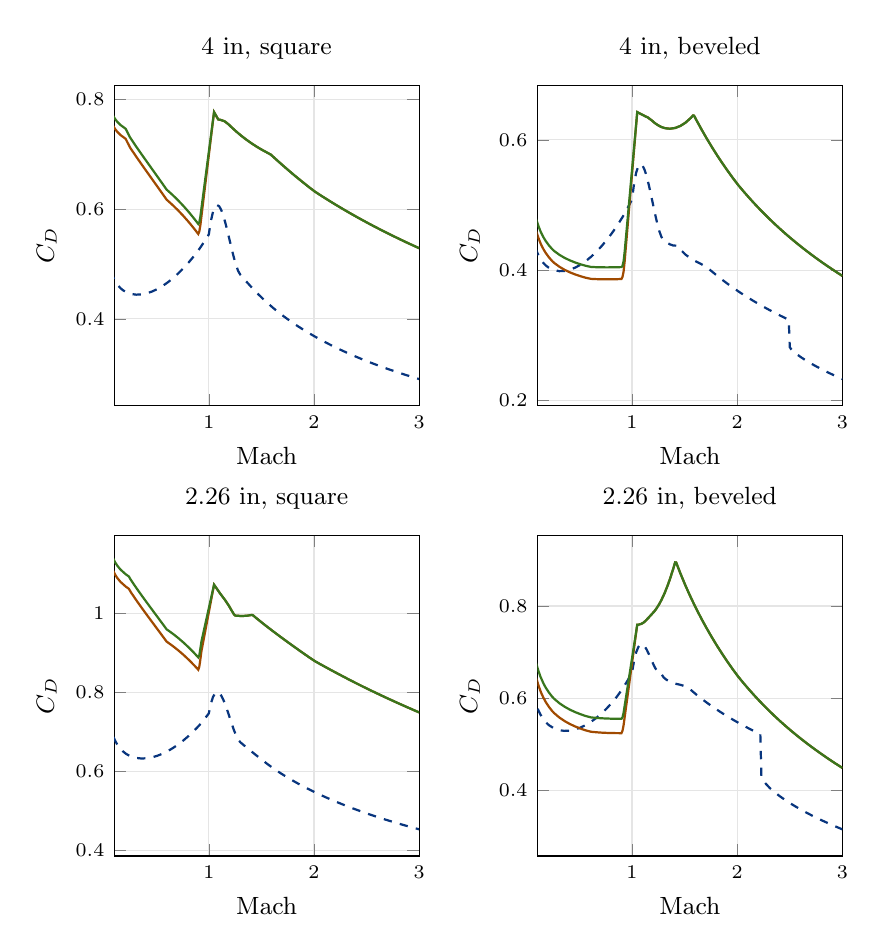
\begin{tikzpicture}
\begin{groupplot}[group style={group size=2 by 2,horizontal sep=1.50cm,vertical sep=1.65cm},width=.45\textwidth,height=5.65cm,grid=major,grid style={gray!20},tick label style={font=\scriptsize},label style={font=\small},title style={font=\small},scaled y ticks=false,yticklabel style={/pgf/number format/fixed,/pgf/number format/precision=3},unbounded coords=jump]
\nextgroupplot[title={4 in, square},xlabel={Mach},ylabel={$C_D$},xmin=0.1,xmax=3]
\addplot[thick,B,dashed] coordinates {(0.01,0.60677) (0.02,0.5556085) (0.03,0.5304755) (0.04,0.514449) (0.05,0.5029597) (0.06,0.494154) (0.07,0.4871088) (0.08,0.4813028) (0.09,0.4764146) (0.11,0.4686128) (0.13,0.4626661) (0.16,0.4560735) (0.18,0.4527952) (0.21,0.4491142) (0.23,0.447324) (0.26,0.4454494) (0.31,0.4440933) (0.36,0.4445371) (0.41,0.4464873) (0.46,0.4497608) (0.51,0.4542372) (0.56,0.4598343) (0.61,0.4664944) (0.66,0.4741763) (0.71,0.4828511) (0.76,0.4924985) (0.81,0.5031053) (0.86,0.5146644) (0.91,0.5273158) (0.96,0.5415691) (1,0.5537129) (1.01,0.5662416) (1.02,0.5785588) (1.04,0.5950453) (1.06,0.6043495) (1.08,0.6073781) (1.1,0.60504) (1.11,0.6013853) (1.12,0.5977591) (1.14,0.5868881) (1.16,0.573339) (1.18,0.5580254) (1.21,0.5338068) (1.22,0.5257669) (1.24,0.5106569) (1.26,0.4974523) (1.28,0.487074) (1.3,0.4804449) (1.31,0.4782286) (1.36,0.4673479) (1.41,0.4568445) (1.46,0.4468198) (1.51,0.4374399) (1.56,0.4285962) (1.61,0.4201874) (1.66,0.4123959) (1.71,0.4049545) (1.76,0.3979763) (1.81,0.3912889) (1.86,0.384968) (1.91,0.3788937) (1.96,0.3731199) (2.01,0.3675585) (2.06,0.3622495) (2.11,0.3571257) (2.16,0.352218) (2.21,0.3474737) (2.26,0.3429169) (2.31,0.3385053) (2.36,0.3342585) (2.41,0.3301417) (2.46,0.3261711) (2.51,0.3223177) (2.56,0.318595) (2.61,0.3149785) (2.66,0.3114796) (2.71,0.3080776) (2.76,0.3047819) (2.81,0.3015749) (2.86,0.2984646) (2.91,0.2954358) (2.96,0.2924953) (3,0.2901949)};
\addplot[thick,burntorange] coordinates {(0.01,0.8495579) (0.02,0.8118115) (0.03,0.7930853) (0.04,0.7810824) (0.05,0.7724362) (0.06,0.7657717) (0.07,0.7604016) (0.08,0.7559364) (0.09,0.7521359) (0.11,0.7459454) (0.13,0.7410526) (0.16,0.7352829) (0.21,0.7282174) (0.25,0.7129462) (0.26,0.710022) (0.31,0.6958134) (0.36,0.6820494) (0.41,0.6685083) (0.46,0.655051) (0.51,0.6415854) (0.56,0.6280468) (0.6,0.6171316) (0.61,0.6155232) (0.66,0.6068493) (0.71,0.5974463) (0.76,0.5872934) (0.81,0.5763745) (0.86,0.5646765) (0.9,0.5547496) (0.91,0.559164) (0.92,0.570585) (0.96,0.6343711) (1.01,0.7135828) (1.05,0.7769522) (1.06,0.7735887) (1.09,0.7635297) (1.11,0.7629026) (1.15,0.7602653) (1.16,0.7587765) (1.19,0.7542984) (1.21,0.7505294) (1.26,0.741705) (1.31,0.733649) (1.36,0.7262857) (1.41,0.7195599) (1.46,0.7133778) (1.51,0.707711) (1.56,0.7025785) (1.59,0.6993915) (1.61,0.6958768) (1.66,0.6872133) (1.71,0.6787261) (1.76,0.6704108) (1.81,0.6622758) (1.86,0.6543916) (1.91,0.646652) (1.96,0.6390482) (2.01,0.6318066) (2.06,0.6255902) (2.11,0.6194991) (2.16,0.6135289) (2.21,0.6076753) (2.26,0.601935) (2.31,0.5963047) (2.36,0.5907947) (2.41,0.5853956) (2.46,0.5801008) (2.51,0.5749075) (2.56,0.5698126) (2.61,0.5648136) (2.66,0.5599076) (2.71,0.5550917) (2.76,0.550363) (2.81,0.5457183) (2.86,0.5411547) (2.91,0.5366689) (2.96,0.5322575) (3,0.5287798)};
\addplot[thick,g] coordinates {(0.01,0.867877) (0.02,0.8301306) (0.03,0.8114044) (0.04,0.7994015) (0.05,0.7907553) (0.06,0.7840908) (0.07,0.7787207) (0.08,0.7742555) (0.09,0.770455) (0.11,0.7642645) (0.13,0.7593717) (0.16,0.753602) (0.21,0.7465365) (0.25,0.7312653) (0.26,0.7283411) (0.31,0.7141325) (0.36,0.7003686) (0.41,0.6868275) (0.46,0.6733701) (0.51,0.6599045) (0.56,0.6463659) (0.6,0.6354507) (0.61,0.6338423) (0.66,0.6251684) (0.71,0.6157654) (0.76,0.6056125) (0.81,0.5946936) (0.86,0.5829956) (0.9,0.5730687) (0.91,0.5762619) (0.92,0.5864615) (0.96,0.6453626) (1.01,0.7184679) (1.05,0.7769522) (1.06,0.7735887) (1.09,0.7635297) (1.11,0.7629026) (1.15,0.7602653) (1.16,0.7587765) (1.19,0.7542984) (1.21,0.7505294) (1.26,0.741705) (1.31,0.733649) (1.36,0.7262857) (1.41,0.7195599) (1.46,0.7133778) (1.51,0.707711) (1.56,0.7025785) (1.59,0.6993915) (1.61,0.6958768) (1.66,0.6872133) (1.71,0.6787261) (1.76,0.6704108) (1.81,0.6622758) (1.86,0.6543916) (1.91,0.646652) (1.96,0.6390482) (2.01,0.6318066) (2.06,0.6255902) (2.11,0.6194991) (2.16,0.6135289) (2.21,0.6076753) (2.26,0.601935) (2.31,0.5963047) (2.36,0.5907947) (2.41,0.5853956) (2.46,0.5801008) (2.51,0.5749075) (2.56,0.5698126) (2.61,0.5648136) (2.66,0.5599076) (2.71,0.5550917) (2.76,0.550363) (2.81,0.5457183) (2.86,0.5411547) (2.91,0.5366689) (2.96,0.5322575) (3,0.5287798)};
\nextgroupplot[title={4 in, beveled},xlabel={Mach},ylabel={$C_D$},xmin=0.1,xmax=3]
\addplot[thick,B,dashed] coordinates {(0.01,0.5613366) (0.02,0.5101743) (0.03,0.4850401) (0.04,0.4690118) (0.05,0.4575203) (0.06,0.4487118) (0.07,0.4416634) (0.08,0.4358537) (0.09,0.4309613) (0.11,0.4231496) (0.13,0.4171912) (0.16,0.4105773) (0.18,0.4072826) (0.21,0.4035737) (0.26,0.399854) (0.31,0.3984336) (0.36,0.3988052) (0.41,0.4006771) (0.46,0.4038687) (0.51,0.4082626) (0.56,0.4137802) (0.61,0.4203684) (0.66,0.4279922) (0.71,0.4366298) (0.76,0.4462704) (0.81,0.4569125) (0.86,0.4685642) (0.91,0.4813849) (0.96,0.4959099) (1,0.5083671) (1.01,0.5206981) (1.02,0.5331006) (1.04,0.5497928) (1.06,0.5593557) (1.08,0.5627033) (1.1,0.5607519) (1.11,0.5573183) (1.12,0.553933) (1.14,0.5436075) (1.16,0.5306963) (1.18,0.5161229) (1.21,0.4932323) (1.22,0.4856999) (1.24,0.4717142) (1.26,0.4597955) (1.28,0.450888) (1.3,0.4459424) (1.31,0.4446585) (1.36,0.4395794) (1.39,0.4379286) (1.41,0.4376369) (1.43,0.4375225) (1.46,0.4315186) (1.51,0.4236521) (1.56,0.4178273) (1.61,0.4132157) (1.66,0.4091312) (1.71,0.4043235) (1.76,0.3979763) (1.81,0.3912889) (1.86,0.384968) (1.91,0.3788937) (1.96,0.3731199) (2.01,0.3675585) (2.06,0.3622495) (2.11,0.3571257) (2.16,0.352218) (2.21,0.3474737) (2.26,0.3429169) (2.31,0.3385053) (2.36,0.3342585) (2.41,0.3301417) (2.46,0.3261711) (2.49,0.3238424) (2.5,0.2818878) (2.51,0.2792915) (2.53,0.2758598) (2.56,0.2717488) (2.61,0.2659186) (2.66,0.260746) (2.71,0.255972) (2.76,0.251504) (2.81,0.2472697) (2.86,0.2432435) (2.91,0.2393876) (2.96,0.2356933) (3,0.2328345)};
\addplot[thick,burntorange] coordinates {(0.01,0.6273081) (0.02,0.5620313) (0.03,0.5299347) (0.04,0.5094494) (0.05,0.4947301) (0.06,0.4834032) (0.07,0.4742865) (0.08,0.4667122) (0.09,0.4602689) (0.1,0.4546867) (0.11,0.4497795) (0.13,0.4414923) (0.14,0.4379393) (0.16,0.4317212) (0.18,0.426426) (0.21,0.4197531) (0.24,0.4141987) (0.26,0.4111535) (0.31,0.4051941) (0.36,0.4004673) (0.41,0.3966106) (0.46,0.3933974) (0.51,0.3906769) (0.56,0.3883444) (0.61,0.3866132) (0.66,0.386218) (0.71,0.3860006) (0.76,0.3859323) (0.81,0.3859904) (0.86,0.3861566) (0.9,0.3863575) (0.91,0.3896268) (0.92,0.3976126) (0.93,0.4129406) (0.96,0.4703392) (1.01,0.5660036) (1.05,0.6425351) (1.06,0.6417257) (1.11,0.6375322) (1.15,0.6344726) (1.16,0.6331312) (1.19,0.6295278) (1.21,0.6266769) (1.23,0.6242195) (1.26,0.6212374) (1.28,0.6197026) (1.31,0.6180618) (1.36,0.6170504) (1.41,0.6181553) (1.46,0.6213053) (1.51,0.6265032) (1.56,0.6338036) (1.58,0.6373163) (1.59,0.6370982) (1.61,0.6309644) (1.66,0.6161905) (1.71,0.6021505) (1.76,0.5887722) (1.81,0.5760099) (1.86,0.5638902) (1.91,0.5522702) (1.96,0.54111) (2.01,0.5305267) (2.06,0.5209216) (2.11,0.5116877) (2.16,0.5028014) (2.21,0.4942413) (2.26,0.4859886) (2.31,0.4780255) (2.36,0.4703494) (2.41,0.4629389) (2.46,0.4557762) (2.51,0.4488485) (2.56,0.4421434) (2.61,0.4356494) (2.66,0.4293556) (2.71,0.4232517) (2.76,0.4173279) (2.81,0.4115746) (2.86,0.4059827) (2.91,0.4005436) (2.96,0.3952487) (3,0.3911112)};
\addplot[thick,g] coordinates {(0.01,0.6456272) (0.02,0.5803504) (0.03,0.5482538) (0.04,0.5277685) (0.05,0.5130492) (0.06,0.5017223) (0.07,0.4926056) (0.08,0.4850313) (0.09,0.478588) (0.1,0.4730058) (0.11,0.4680986) (0.13,0.4598114) (0.14,0.4562584) (0.16,0.4500403) (0.18,0.4447451) (0.21,0.4380722) (0.24,0.4325179) (0.26,0.4294726) (0.31,0.4235133) (0.36,0.4187864) (0.41,0.4149297) (0.46,0.4117165) (0.51,0.408996) (0.56,0.4066635) (0.61,0.4049323) (0.66,0.4045371) (0.71,0.4043197) (0.76,0.4042514) (0.81,0.4043095) (0.86,0.4044758) (0.9,0.4046766) (0.91,0.4067247) (0.92,0.4134891) (0.93,0.4275959) (0.96,0.4813307) (1.01,0.5708887) (1.05,0.6425351) (1.06,0.6417257) (1.11,0.6375322) (1.13,0.635746) (1.15,0.6344726) (1.16,0.6331312) (1.19,0.6295278) (1.21,0.6266769) (1.23,0.6242195) (1.26,0.6212374) (1.28,0.6197026) (1.31,0.6180618) (1.33,0.617401) (1.36,0.6170504) (1.41,0.6181553) (1.46,0.6213053) (1.51,0.6265032) (1.56,0.6338036) (1.58,0.6373163) (1.59,0.6370982) (1.61,0.6309644) (1.66,0.6161905) (1.71,0.6021505) (1.76,0.5887722) (1.81,0.5760099) (1.86,0.5638902) (1.91,0.5522702) (1.96,0.54111) (2.01,0.5305267) (2.06,0.5209216) (2.11,0.5116877) (2.16,0.5028014) (2.21,0.4942413) (2.26,0.4859886) (2.31,0.4780255) (2.36,0.4703494) (2.41,0.4629389) (2.46,0.4557762) (2.51,0.4488485) (2.56,0.4421434) (2.61,0.4356494) (2.66,0.4293556) (2.71,0.4232517) (2.76,0.4173279) (2.81,0.4115746) (2.86,0.4059827) (2.91,0.4005436) (2.96,0.3952487) (3,0.3911112)};
\nextgroupplot[title={2.26 in, square},xlabel={Mach},ylabel={$C_D$},xmin=0.1,xmax=3]
\addplot[thick,B,dashed] coordinates {(0.01,0.8946718) (0.02,0.8141892) (0.03,0.774762) (0.04,0.7496437) (0.05,0.7316345) (0.06,0.717819) (0.07,0.7067476) (0.08,0.6976021) (0.09,0.6898785) (0.11,0.6774776) (0.13,0.6679211) (0.16,0.6571194) (0.18,0.6515945) (0.21,0.6451364) (0.23,0.6418) (0.26,0.6379607) (0.31,0.634055) (0.36,0.6326271) (0.41,0.6332196) (0.46,0.6355476) (0.51,0.6394233) (0.56,0.6447183) (0.61,0.6513418) (0.66,0.6592287) (0.71,0.6683317) (0.76,0.6786169) (0.81,0.69006) (0.86,0.7026445) (0.91,0.7165768) (0.96,0.7326736) (1,0.7465538) (1.01,0.759381) (1.02,0.7716649) (1.04,0.7881295) (1.06,0.797468) (1.08,0.8005841) (1.1,0.798384) (1.11,0.7946924) (1.12,0.7910349) (1.14,0.780117) (1.16,0.7665392) (1.18,0.7512114) (1.21,0.7269912) (1.24,0.7038515) (1.26,0.690653) (1.28,0.6802751) (1.3,0.6736352) (1.31,0.6714077) (1.36,0.6603849) (1.41,0.6495222) (1.46,0.6388059) (1.51,0.6282816) (1.56,0.6181158) (1.61,0.6083982) (1.66,0.5994216) (1.71,0.5908014) (1.76,0.582722) (1.81,0.5749378) (1.86,0.5675743) (1.91,0.5604617) (1.96,0.5536906) (2.01,0.5471371) (2.06,0.5408691) (2.11,0.5347927) (2.16,0.5289603) (2.21,0.5232985) (2.26,0.5178489) (2.31,0.5125527) (2.36,0.5074434) (2.41,0.502473) (2.46,0.4976692) (2.51,0.492992) (2.56,0.4884644) (2.61,0.4840529) (2.66,0.4797768) (2.71,0.4756075) (2.76,0.4715615) (2.81,0.4676142) (2.86,0.4637798) (2.91,0.4600369) (2.96,0.4563977) (3,0.4535445)};
\addplot[thick,burntorange] coordinates {(0.01,1.267614) (0.02,1.206184) (0.03,1.175521) (0.04,1.155777) (0.05,1.1415) (0.06,1.130461) (0.07,1.12154) (0.08,1.114104) (0.09,1.10776) (0.11,1.097395) (0.13,1.089171) (0.16,1.079435) (0.21,1.067446) (0.24,1.061856) (0.26,1.05284) (0.31,1.03323) (0.36,1.014474) (0.41,0.9962033) (0.46,0.9781847) (0.51,0.9602636) (0.56,0.9423313) (0.6,0.9279242) (0.61,0.9261832) (0.66,0.9165992) (0.71,0.9060866) (0.76,0.8946104) (0.81,0.8821426) (0.86,0.8686612) (0.9,0.8571339) (0.91,0.8646967) (0.92,0.8832203) (0.93,0.9036087) (0.96,0.9457067) (1.01,1.01587) (1.05,1.072001) (1.06,1.068198) (1.11,1.049109) (1.16,1.031324) (1.19,1.019307) (1.21,1.010021) (1.24,0.9967948) (1.25,0.9941698) (1.26,0.9937856) (1.31,0.9928582) (1.36,0.993518) (1.41,0.9956987) (1.42,0.9946646) (1.46,0.9858597) (1.51,0.9751363) (1.56,0.9647068) (1.61,0.954515) (1.66,0.9445196) (1.71,0.9346895) (1.76,0.9250006) (1.81,0.915434) (1.86,0.9059753) (1.91,0.8966132) (1.96,0.887339) (2.01,0.878497) (2.06,0.8710869) (2.11,0.8637671) (2.16,0.8565376) (2.21,0.8493984) (2.26,0.84235) (2.31,0.8353926) (2.36,0.8285268) (2.41,0.8217523) (2.46,0.815114) (2.51,0.8085912) (2.56,0.8021579) (2.61,0.7958132) (2.66,0.7895553) (2.71,0.7833824) (2.76,0.777292) (2.81,0.7712813) (2.86,0.7653475) (2.91,0.7594869) (2.96,0.7536959) (3,0.7491106)};
\addplot[thick,g] coordinates {(0.01,1.298716) (0.02,1.237287) (0.03,1.206623) (0.04,1.186879) (0.05,1.172603) (0.06,1.161563) (0.07,1.152643) (0.08,1.145206) (0.09,1.138862) (0.11,1.128497) (0.13,1.120274) (0.16,1.110537) (0.21,1.098548) (0.24,1.092959) (0.26,1.083943) (0.31,1.064332) (0.36,1.045577) (0.41,1.027306) (0.46,1.009287) (0.51,0.9913659) (0.56,0.9734337) (0.6,0.9590265) (0.61,0.9572855) (0.66,0.9477015) (0.71,0.9371889) (0.76,0.9257127) (0.81,0.9132449) (0.86,0.8997635) (0.9,0.8882362) (0.91,0.8937256) (0.92,0.9101757) (0.93,0.9284905) (0.96,0.9643681) (1.01,1.024164) (1.05,1.072001) (1.06,1.068198) (1.11,1.049109) (1.16,1.031324) (1.19,1.019307) (1.21,1.010021) (1.24,0.9967948) (1.25,0.9941698) (1.26,0.9937856) (1.31,0.9928582) (1.36,0.993518) (1.41,0.9956987) (1.42,0.9946646) (1.46,0.9858597) (1.51,0.9751363) (1.56,0.9647068) (1.61,0.954515) (1.66,0.9445196) (1.71,0.9346895) (1.76,0.9250006) (1.81,0.915434) (1.86,0.9059753) (1.91,0.8966132) (1.96,0.887339) (2.01,0.878497) (2.06,0.8710869) (2.11,0.8637671) (2.16,0.8565376) (2.21,0.8493984) (2.26,0.84235) (2.31,0.8353926) (2.36,0.8285268) (2.41,0.8217523) (2.46,0.815114) (2.51,0.8085912) (2.56,0.8021579) (2.61,0.7958132) (2.66,0.7895553) (2.71,0.7833824) (2.76,0.777292) (2.81,0.7712813) (2.86,0.7653475) (2.91,0.7594869) (2.96,0.7536959) (3,0.7491106)};
\nextgroupplot[title={2.26 in, beveled},xlabel={Mach},ylabel={$C_D$},xmin=0.1,xmax=3]
\addplot[thick,B,dashed] coordinates {(0.01,0.7914273) (0.02,0.7109446) (0.03,0.6715172) (0.04,0.6463985) (0.05,0.6283889) (0.06,0.6145729) (0.07,0.603501) (0.08,0.5943548) (0.09,0.5866306) (0.11,0.5742283) (0.13,0.5646703) (0.16,0.5538668) (0.18,0.5483412) (0.21,0.5418833) (0.26,0.5347138) (0.31,0.5308263) (0.36,0.5294353) (0.41,0.5300926) (0.46,0.5325241) (0.51,0.5365565) (0.56,0.5420788) (0.61,0.549023) (0.66,0.5573528) (0.71,0.5670577) (0.76,0.5781515) (0.81,0.5906725) (0.86,0.6046876) (0.91,0.6205165) (0.96,0.639133) (1,0.6556257) (1.01,0.6685444) (1.02,0.6815933) (1.04,0.6997682) (1.06,0.7110903) (1.08,0.7165072) (1.1,0.7169756) (1.11,0.7147743) (1.12,0.7127224) (1.14,0.7054007) (1.16,0.6960095) (1.21,0.6703572) (1.22,0.6658697) (1.24,0.6589052) (1.26,0.6555737) (1.27,0.6561345) (1.3,0.6455585) (1.31,0.6434793) (1.33,0.6399143) (1.36,0.6358956) (1.41,0.6318494) (1.46,0.6292845) (1.51,0.6256545) (1.54,0.6217974) (1.56,0.6181158) (1.61,0.6083982) (1.66,0.5994216) (1.71,0.5908014) (1.76,0.582722) (1.81,0.5749378) (1.86,0.5675743) (1.91,0.5604617) (1.96,0.5536906) (2.01,0.5471371) (2.06,0.5408691) (2.11,0.5347927) (2.16,0.5289603) (2.21,0.5232985) (2.22,0.5221971) (2.23,0.4300758) (2.24,0.4246674) (2.26,0.4178673) (2.31,0.4056283) (2.36,0.3957804) (2.41,0.3870748) (2.46,0.3791475) (2.51,0.371771) (2.56,0.3648606) (2.61,0.3583144) (2.66,0.3521046) (2.71,0.3461686) (2.76,0.3404976) (2.81,0.335047) (2.86,0.3298156) (2.91,0.3247691) (2.96,0.3199093) (3,0.3161335)};
\addplot[thick,burntorange] coordinates {(0.01,0.9035057) (0.02,0.8030635) (0.03,0.7534984) (0.04,0.7217787) (0.05,0.6989371) (0.06,0.6813263) (0.07,0.6671282) (0.08,0.6553145) (0.09,0.6452512) (0.1,0.6365217) (0.11,0.6288388) (0.13,0.6158435) (0.14,0.6102636) (0.16,0.6004849) (0.18,0.5921437) (0.21,0.5816123) (0.24,0.572828) (0.26,0.5679674) (0.31,0.5583297) (0.36,0.550634) (0.41,0.5443128) (0.46,0.5390101) (0.51,0.5344889) (0.56,0.5305844) (0.61,0.5275777) (0.66,0.5264764) (0.71,0.5256663) (0.76,0.525101) (0.81,0.5247437) (0.86,0.5245652) (0.9,0.5245348) (0.91,0.529836) (0.92,0.5415746) (0.96,0.6085702) (1.01,0.6924451) (1.05,0.7595449) (1.06,0.7594329) (1.09,0.7614603) (1.11,0.7641062) (1.13,0.768068) (1.16,0.7753619) (1.21,0.7878109) (1.23,0.7936705) (1.26,0.8044868) (1.28,0.813036) (1.31,0.8278553) (1.34,0.8450646) (1.36,0.8578667) (1.39,0.8790701) (1.41,0.8945451) (1.42,0.8943775) (1.46,0.870722) (1.51,0.8433653) (1.56,0.8180788) (1.61,0.7945187) (1.66,0.7724305) (1.71,0.7516192) (1.76,0.7319308) (1.81,0.7132413) (1.86,0.6954483) (1.91,0.6784663) (1.96,0.6622224) (2.01,0.6468749) (2.06,0.6329977) (2.11,0.6197009) (2.16,0.6069438) (2.21,0.5946903) (2.26,0.5829078) (2.31,0.5715667) (2.36,0.5606401) (2.41,0.5501028) (2.46,0.5399768) (2.51,0.5302207) (2.56,0.5207892) (2.61,0.5116636) (2.66,0.5028262) (2.71,0.4942602) (2.76,0.4859493) (2.81,0.4778783) (2.86,0.4700325) (2.91,0.4623978) (2.96,0.4549605) (3,0.4491439)};
\addplot[thick,g] coordinates {(0.01,0.934608) (0.02,0.8341658) (0.03,0.7846007) (0.04,0.7528811) (0.05,0.7300394) (0.06,0.7124286) (0.07,0.6982305) (0.08,0.6864168) (0.09,0.6763535) (0.1,0.667624) (0.11,0.6599411) (0.13,0.6469458) (0.16,0.6315872) (0.18,0.623246) (0.21,0.6127146) (0.24,0.6039303) (0.26,0.5990697) (0.31,0.589432) (0.36,0.5817363) (0.41,0.5754151) (0.46,0.5701124) (0.51,0.5655912) (0.56,0.5616867) (0.61,0.55868) (0.66,0.5575787) (0.71,0.5567686) (0.76,0.5562033) (0.81,0.555846) (0.86,0.5556675) (0.9,0.5556371) (0.91,0.5588648) (0.92,0.5685299) (0.96,0.6272316) (1.01,0.700739) (1.05,0.7595449) (1.06,0.7594329) (1.09,0.7614603) (1.11,0.7641062) (1.13,0.768068) (1.16,0.7753619) (1.21,0.7878109) (1.23,0.7936705) (1.26,0.8044868) (1.28,0.813036) (1.31,0.8278553) (1.34,0.8450646) (1.36,0.8578667) (1.39,0.8790701) (1.41,0.8945451) (1.42,0.8943775) (1.46,0.870722) (1.51,0.8433653) (1.56,0.8180788) (1.61,0.7945187) (1.66,0.7724305) (1.71,0.7516192) (1.76,0.7319308) (1.81,0.7132413) (1.86,0.6954483) (1.91,0.6784663) (1.96,0.6622224) (2.01,0.6468749) (2.06,0.6329977) (2.11,0.6197009) (2.16,0.6069438) (2.21,0.5946903) (2.26,0.5829078) (2.31,0.5715667) (2.36,0.5606401) (2.41,0.5501028) (2.46,0.5399768) (2.51,0.5302207) (2.56,0.5207892) (2.61,0.5116636) (2.66,0.5028262) (2.71,0.4942602) (2.76,0.4859493) (2.81,0.4778783) (2.86,0.4700325) (2.91,0.4623978) (2.96,0.4549605) (3,0.4491439)};
\end{groupplot}\end{tikzpicture}
\caption{Default and modified RAS settings share geometry and drag-flow inputs. This isolates the normal-force/body-interference option, compared with unmodified MIT OR.}\label{fig:atlas-26-rogers-CD}
\end{figure}
\noindent{\footnotesize Export files: \code{26-rogers-CD.svg} and \code{26-rogers-CD.png}.\\ Directory: \code{aerodynamic-investigation/extended/figures/}.}

\end{document}
